\RequirePackage[l2tabu,orthodox]{nag} % for package advice

% TODO: decide if one-sided/two-sided
% \documentclass[headsepline,footsepline,footinclude=false,fontsize=11pt,paper=a4,listof=totoc,bibliography=totoc,BCOR=12mm,DIV=12]{scrbook} % two-sided
\documentclass[headsepline,footsepline,footinclude=false,oneside,fontsize=11pt,paper=a4,listof=totoc,bibliography=totoc]{scrbook} % one-sided

\PassOptionsToPackage{table,svgnames,dvipsnames}{xcolor}

% general/language
\usepackage[utf8]{inputenc}
\usepackage[T1]{fontenc}
\usepackage[sc]{mathpazo}
\usepackage[american]{babel}
\usepackage[autostyle]{csquotes}
\usepackage[%
  backend=bibtex,
  url=false,
  doi=false,
  style=numeric,
  giveninits,
  sorting=none,
  maxnames=10
]{biblatex}
\usepackage{booktabs} % for rulers in tables
\usepackage[final]{microtype} % for \microtypesetup{protrusion=true}
\usepackage[hidelinks, breaklinks = true]{hyperref} % hidelinks removes colored boxes around references and links, breaklinks allows linebreak in e.g. list of figures for long captions
%\usepackage[toc,nonumberlist,acronym]{glossaries} % TODO: remove if glossary not needed

% math
\usepackage{amsmath}
\usepackage{algorithm} %for algorithm environment
\usepackage{algpseudocode} %for algorithm environment
\usepackage{units} % for units
%\usepackage{scrhack} % necessary for listings package
%\usepackage{listings}

% graphics
\usepackage{graphicx}
\usepackage{psfrag}
\usepackage{epstopdf}
\usepackage{tikz}
\usepackage{lmodern}
\usepackage{pgf}
\usepackage{pgfplots}
\usepackage{pgfplotstable}

\usepackage{caption} % Required for custom captions
\usepackage{subcaption} % Required for subfigures


% Basic information for cover & title page
\newcommand*{\getUniversity}{Technical University of Munich} %{Technische Universität München}
\newcommand*{\getFaculty}{Department of Informatics}
\newcommand*{\getTitle}{Realistic Optimization-based Driving Using a Constrained Double-Integrator Model}
\newcommand*{\getTitleGer}{Realistisches, optimierungsbasiertes Fahren mit einem beschränkten Doppel Integrator Modell}
\newcommand*{\getAuthor}{Andreas Belavic}
\newcommand*{\getDoctype}{Bachelor's Thesis in Informatics}
\newcommand*{\getSupervisor}{Prof.
	Dr.-Ing.
	Matthias Althoff} \newcommand*{\getAdvisor}{M.Sc.
	Tobias Mascetta, M.Sc.
	Lukas Schäfer}
\newcommand*{\getSubmissionDate}{28.02.2025}
\newcommand*{\getSubmissionLocation}{Munich}

\newcommand{\arstretch}[1]{\renewcommand{\arraystretch}{#1}} %to change the row spacing in tables
% TODO: add custom commands etc.

% Settings for bibliography
\bibliography{content/literature}
% \addbibresource{content/literature}

% Settings for fonts
\setkomafont{disposition}{\normalfont\bfseries} % use serif font for headings
\linespread{1.05} % adjust line spread for mathpazo font

% Settings for glossaries
%\renewcommand{\glsnamefont}[1]{\normalfont\bfseries #1} % use serif font for glossary entry titles
%\makeglossaries{}

% Settings for pgfplots
\pgfplotsset{compat=1.9} % TODO: adjust to your installed version
\pgfplotsset{
	% For available color names, see http://www.latextemplates.com/svgnames-colors
	cycle list={CornflowerBlue\\Dandelion\\ForestGreen\\BrickRed\\},
}

% Settings for lstlistings
%\lstset{%
%  basicstyle=\ttfamily,
%  columns=fullflexible,
%  autogobble,
%  keywordstyle=\bfseries\color{MediumBlue},
%  stringstyle=\color{DarkGreen}
%}
% \newglossaryentry{computer}
{
  name=computer,
  description={is a machine that\ldots}
}
 % TODO: uncomment if glossary needed
% \newacronym{tum}{TUM}{Technische Universität München}
 % TODO: uncomment if list of abbreviations needed

\def\mathdefault#1{#1}
\everymath=\expandafter{\the\everymath\displaystyle}

\ifdefined\pdftexversion\else  % non-pdftex case.
	\usepackage{fontspec}
\fi
\makeatletter\@ifpackageloaded{underscore}{}{\usepackage[strings]{underscore}}\makeatother

\begin{document}
\begin{titlepage}
  % HACK for two-sided documents: ignore binding correction for cover page.
  % Adapted from Markus Kohm's KOMA-Script titlepage=firstiscover handling.
  % See http://mirrors.ctan.org/macros/latex/contrib/koma-script/scrkernel-title.dtx,
  % \maketitle macro.
  \oddsidemargin=\evensidemargin\relax
  \textwidth=\dimexpr\paperwidth-2\evensidemargin-2in\relax
  \hsize=\textwidth\relax

  \centering

  \vspace{40mm}
  
\includegraphics[width=40mm]{./figures/tum}

  \vspace{5mm}
  {\LARGE \MakeUppercase{\getUniversity{}}}\\

  \vspace{5mm}
  {\Large \MakeUppercase{\getFaculty{}}}\\

  \vspace{20mm}
  {\Large \getDoctype{}}

  \vspace{15mm}
  {\huge\bfseries \getTitle{}}

  \vspace{15mm}
  {\LARGE \getAuthor{}}

  \vspace{20mm}
  %
\includegraphics[width=20mm]{logos/faculty}
	
\end{titlepage}


\frontmatter{}
\begin{titlepage}
  \centering

  \vspace{40mm}
  
\includegraphics[width=40mm]{./figures/tum}

  \vspace{5mm}
  {\LARGE \MakeUppercase{\getUniversity{}}}\\

  \vspace{5mm}
  {\Large \MakeUppercase{\getFaculty{}}}\\

  \vspace{20mm}
  {\Large \getDoctype{}}

  \vspace{15mm}
  {\huge\bfseries \getTitle{}}

  \vspace{10mm}
  {\huge\bfseries \getTitleGer{}}

  \vspace{15mm}
  \begin{tabular}{l l}
    Author:          & \getAuthor{}         \\
    Supervisor:      & \getSupervisor{}     \\
    Advisor:         & \getAdvisor{}        \\
    Submission Date: & \getSubmissionDate{} \\
  \end{tabular}

  \vspace{20mm}
  %
\includegraphics[width=20mm]{logos/faculty}
\end{titlepage}

\thispagestyle{empty}
\vspace*{0.65\textheight}
\noindent
I confirm that this bachelor's thesis is my own work and I have documented all sources and material used. \\\\
Ich versichere, dass ich diese Bachelor's Thesis selbständig verfasst und nur die angegebenen Quellen und Hilfsmittel verwendet habe.

\vspace{15mm}
\noindent
\getSubmissionLocation{}, \getSubmissionDate{} \hspace{5cm} \getAuthor{}

\cleardoublepage{}

% \addcontentsline{toc}{chapter}{Acknowledgments}
\thispagestyle{empty}

\vspace*{2cm}

\begin{center}
{\usekomafont{section} Acknowledgments}
\end{center}

\vspace{1cm}

A thesis may include an acknowledgments section where the author may want to thank certain people, groups, institutions, etc. who provided support.


\cleardoublepage{}

\chapter{\abstractname}
This is the abstract.
It is a short summary of your work, consisting of roughly one to three paragraphs.
It should give the main ideas of your paper, i.e., the posed problem, a motivation for solving it, your solution method, and your results results
results.
Keep it understandable for a general audience.
Do not include references.

\microtypesetup{protrusion=false}
\tableofcontents{}
\microtypesetup{protrusion=true}

\mainmatter{}
\chapter{Introduction}
\section{Overview} \label{sec:overview}

\begin{figure}[b]
	\centering
	\begin{tikzpicture}[
			node distance=1cm,
			auto,
			thick,
			box/.style={rectangle, draw, text width=2cm, align=center, rounded corners, minimum height=1.5cm},
			arrow/.style={-Latex, thick},
			label/.style={font=\small, text width=2cm, align=center},
			highlighted/.style={fill=blue!30, font=\bfseries}
		]
		% Nodes
		\node[box] (route) {Route Planning};
		\node[box] (behavior) [right=of route] {Behavioral Layer};
		\node[box] (motion) [right=of behavior, highlighted] {Motion Planning Layer};
		\node[box] (local) [right=of motion] {Local Feedback};

		% Initial and final arrows
		\draw[arrow] (-2, 0) -- (route.west);
		\draw[arrow] (route.east) -- (behavior.west);
		\draw[arrow] (behavior.east) -- (motion.west);
		\draw[arrow] (motion.east) -- (local.west);
		\draw[arrow] (local.east) -- (11.8, 0);

		% Text labels below arrows
		% \node[label] at (-1.2, -1.25) {Destination};
		% \node[label] at (11.2, -1.25) {Control Commands};

	\end{tikzpicture}
	\caption{Overview of Motion Planning Problem Decomposition}
	\label{fig:motion_planning_overview}
\end{figure}

The motion planning system for autonomous driving is typically organized into a hierarchical, layered architecture that efficiently handles both
large-scale navigation and local trajectory optimization.
Figure \ref{fig:motion_planning_overview} illustrates this decomposition, adapted from ~\cite{paden_survey_2016}, and emphasizes the motion planning
layer, which is the focus of this work.

At the highest level, the Route Planning component takes a user-specified destination and uses search- or graph-based methods to generate a
high-level route through the road network.
This global planner addresses large-scale navigation by selecting a sequence of waypoints that outline the overall path from the start location to
the destination.

Following route planning, the Behavioral Layer refines the generated waypoints by incorporating environmental factors such as other vehicles,
obstacles, and road signs.
This step ensures that the vehicle adapts to dynamic traffic conditions and selects a behavioral strategy appropriate for the current driving
context.

Once the behavioral strategy is set, the Motion Planning Layer takes center stage.
Building on insights from early demonstrations in the DARPA Grand and Urban Challenges \cite{thrun_stanley_2006,montemerlo_junior_2008}, the motion
planning literature has evolved to tackle a wide variety of environments—from structured highways and urban roads to unstructured parking lots and
off-road terrains.
A unifying theme across these scenarios is the production of collision-free, dynamically feasible trajectories that account for comfort and
operational constraints.

In this context, an optimization-based local planner refines the global route into a smooth, continuous guiding trajectory in real
time~\cite{van_hierarchical_2020}.
Unlike the global route—represented as a series of discrete waypoints—this trajectory not only satisfies road rules and safety constraints but also
ensures fluid, comfortable motion that adapts to dynamic obstacles, road curvature, and other real-time factors.

Another critical element in the motion planning pipeline is the vehicle model.
This model defines the vehicle's position and orientation in the real world and predicts how these states evolve over time.
The choice of vehicle model significantly impacts both the accuracy and the computational complexity of the planning process: simpler models offer
efficiency at the cost of precision, whereas more complex models yield higher fidelity with increased computational demands.

Finally, the Local Feedback component executes the planned trajectory by generating precise control commands—steering, throttle, and brake
inputs—based on real-time vehicle and environmental feedback.
This closed-loop control ensures that the trajectory is followed accurately, even as conditions evolve.

% Next, the Behavioral Layer refines these waypoints by considering environmental factors such as other vehicles, obstacles, and road signs, ensuring
% the vehicle adapts to dynamic traffic conditions.
% Once a behavioral strategy is determined, the Motion Planning Layer takes center stage.
% Building on insights from early demonstrations in the DARPA Grand and Urban Challenges \cite{thrun_stanley_2006,montemerlo_junior_2008}, the motion
% planning literature has evolved to handle a wide variety of environments—from structured highways and urban roads to unstructured parking lots and
% off-road terrains.
% A unifying theme across these scenarios is the need to produce collision-free, dynamically feasible trajectories that also account for comfort and
% operational constraints.

% In this context, an optimization-based local planner refines the global route into a dynamically feasible, collision-free trajectory in real time
% \cite{van_hierarchical_2020}.
% Unlike the global route, which is represented as a series of waypoints, the resulting trajectory is a smooth, continuous guiding curve.
% It not only ensures compliance with road rules and safety constraints but also guarantees a fluid and comfortable motion that adapts to dynamic
% obstacles, road curvature, and other real-time factors.

% Another critical element in the motion planning pipeline is the vehicle model, which defines the position and orientation of the vehicle in the real
% world and predicts how these states evolve over time.
% The choice of model significantly impacts both the accuracy and computational complexity of the planning process.
% While simpler models are computationally efficient, they may lack precision; conversely, more complex models provide higher fidelity at the cost of
% increased computational resources.

% Finally, the Local Feedback component executes the plan by generating precise control commands—steering, throttle, and brake inputs—based on
% real-time vehicle and environmental feedback, ensuring that the trajectory is followed accurately.

% The motion planning problem can be divided into four main components, each representing an essential aspect of the system.
% Figure \ref{fig:motion_planning_overview} illustrates this decomposition, adapted from \cite{paden_survey_2016}, with an emphasis on the motion
% planning layer, which is the focus of this work.

% The process begins with the user providing a travel destination, which serves as the input to the Route Planning component.
% This phase generates a sequence of waypoints through a predefined road network.
% Next, the Behavioral Layer refines the waypoints by considering environmental factors such as other vehicles, obstacles, and road signs, ensuring the
% vehicle adapts to dynamic traffic conditions.
% Once a behavioral strategy is determined, the Motion Planning Layer generates a trajectory that satisfies physical and safety constraints, ensuring
% feasibility and compliance with road rules.
% Finally, the Local Feedback component executes the plan by generating precise control commands—steering, throttle, and brake inputs—based on
% real-time vehicle and environmental feedback.

Finding an exact solution to the motion planning problem is computationally intractable in most cases.
As a result, numerical methods are commonly used to approximate solutions.
These approaches fall into three main categories:

\begin{enumerate}
	\item Graph-Based Algorithms discretize the vehicle's state space and connect valid
	      transitions with edges, allowing a graph search algorithm to determine an optimal
	      trajectory

	\item Incremental Tree Approaches expand a search tree by randomly applying control
	      commands and simulating state transitions until a feasible trajectory is found.

	\item Optimization-Based Methods formulate the problem as an optimization task over a function space, minimizing an objective function (e.g., travel time, energy efficiency)
	      while respecting constraints.
\end{enumerate}

We focus on optimization-based motion planning, which offers a structured and efficient approach to trajectory generation while ensuring collision
avoidance and adherence to vehicle dynamics.
Compared to graph-based or Incremental Tree approaches, optimization-based methods provide smoother and more dynamically feasible trajectories by
directly incorporating vehicle dynamics constraints.
Additionally, they offer deterministic performance with guaranteed feasibility, avoiding the sampling inconsistencies and discontinuities often found
in tree-based methods.
By leveraging convex optimization and constraint reformulation, this approach efficiently computes safe and feasible trajectories while maintaining
real-time performance in dynamic environments.

Building on these advantages, we review existing optimization-based motion planning approaches, highlighting key methodologies, challenges, and
advancements in the field.

\section{Related Work} \label{sec:related_work}

\section{Problem Formulation} \label{sec:convex_discrete_time_optimization}

Motion planning for autonomous vehicles must simultaneously address two fundamental challenges: ensuring collision-free trajectories and accurately
capturing the vehicle's dynamic behavior.
In this section, we introduce a discrete-time formulation of the trajectory planning problem and discuss its inherent computational complexity.
This lays the groundwork for our convex optimization approach.

\subsection{Computational Complexity} \label{subsec:complexity}

Optimal trajectory planning is computationally intractable and classified as PSPACE-Hard \cite{reif_complexity_1979}, with resource requirements
growing exponentially with problem size.
This complexity arises from the continuous state space, non-convex vehicle dynamics constraints, and the need to enforce collision avoidance while
satisfying dynamic constraints.
These challenges, akin to the classic Movers' Problem, are further complicated by time dependencies and evolving vehicle behavior.
Exact solutions are impractical for real-time use, necessitating numerical optimization, heuristics, or approximate solvers for efficient
near-optimal solutions.

\subsection{Discrete-Time Problem Formulation}

To render the trajectory planning problem tractable, we discretize the continuous-time formulation into a finite set of time steps.
Let $\mathcal{X}$ denote the set of valid vehicle states and $\mathcal{U}$ the set of feasible control inputs.
We define the trajectory at discrete time points $\{t_i\}_{i=1,\dots ,m}$, with the state at time $t_i$ denoted by $\pi(t_i) = x_i$.
Our objective is to minimize a cumulative cost function $ J: \mathcal{X} \times \mathcal{U} \to \mathbb{R}, $ which penalizes deviations from desired
behaviors, including collisions and dynamic infeasibilities.

\subsubsection{Discrete-Time Optimal Trajectory Planning}\label{subsubsec:discrete_time_optimal_trajectory_planning}

Given a 7-tuple
$
	(\mathcal{X}, \mathcal{U}, x_{\text{initial}}, X_{\text{goal}}, f, J, \{t_i\}_{i=1,\dots ,m}),
$
the discrete-time optimal trajectory planning problem is defined as:
\begin{align}
	u^*     & = \underset{u \in \mathcal{U}^{m-1}}{\operatorname{arg\,min}} \sum_{i=1}^{m-1}
	J(x_{i+1}, u_{i}), \label{eq:obj}                                                                                                                                   \\ \text{s.t.
	} \quad & x_1  = x_{\text{initial}} \label{eq:init}                                                                                                                 \\
	        & x_m          \in X_{\text{goal}} \subseteq \mathcal{X} \label{eq:goal}                                                                                    \\
	        & (x_i, u_i)   \in \mathcal{C} \subseteq \mathcal{X} \times \mathcal{U}          & \text{for all}\, i \in \{1, \dots, m-1\} \label{eq:coupling_constraints} \\
	        & x_{i+1}      = x_i + \Delta t_i \, f(x_i, u_i)                                 & \text{for all}\, i \in \{1, \dots, m-1\} \label{eq:discrete_dynamics}
\end{align}
where $\Delta t_i = t_{i+1} - t_i$, and $\mathcal{C}$ represents the set of coupling constraints that jointly enforce collision avoidance and the vehicle's dynamic limitations.
The system dynamics are approximated using an integration scheme, as specified in \eqref{eq:discrete_dynamics}, which estimates the state at time
$t_{i+1}$ based on the state at time $t_i$ and the control input $u_i$.

\subsubsection{Disciplined Convex Programming (DCP)}

The DCP framework imposes specific rules on how optimization problems must be formulated, which helps in verifying the convexity of the problem and
guarantees that the problem can be solved efficiently.
The key principles of DCP are as follows:
\begin{itemize}
	\item The objective function must be convex over the feasible set if it is to be minimized, or concave if it is to
	      be maximized.
	\item Constraints must be formulated in one of the following forms:
	      \begin{itemize}
		      \item An equality constraint between affine expressions: \(\text{affine} = \text{affine}\),
		      \item An inequality constraint where a convex function is bounded above by a concave function: \(\text{convex} \leq \text{concave}\).
	      \end{itemize}
\end{itemize}
The use of DCP in this work involves defining the cost function and constraints in a manner that satisfies the DCP rules.
We will use the term \textit{convex constraint} or \textit{convex form} to refer to constraints that adhere to these rules.

\section{Thesis Structure} \label{sec:thesis_structure}
Chapter 2 introduces the vehicle modeling approaches such as the double integrator and bicycle models.
Chapter 3 presents the proposed motion planning methods, detailing coordinate transformations, constraint formulations, model dynamics
approximations, and convex relaxation techniques.
It also explores various modeling strategies, including soft constraints and auxiliary variables.
Chapter 4 focuses on the implementation and evaluation of the proposed methods, describing performance analysis, simulation results, and challenges.
Chapter 5 discusses the findings, their implications, and possible improvements, outlining future research directions.
Finally, Chapter 6 concludes the thesis by summarizing its key contributions and highlighting the broader impact of the research.


\chapter{Preliminaries}
\section{Vehicle Models} \label{sec:vehicle_models}

A vehicle model defines the position and orientation of a vehicle in the real world and predicts how these states evolve over time.
The choice of model significantly impacts the accuracy and computational complexity of motion planning.
Simpler models, while computationally efficient, may lack precision, whereas more complex models provide higher fidelity but require greater
computational resources.

This section introduces two fundamental models used in trajectory planning [15]: the point mass model, which provides a simplified kinematic
representation, and the bicycle model, which captures essential vehicle dynamics.
In both models, the system's state is represented by a vector $x$, containing relevant variables such as position, velocity, and orientation, while
the control inputs, represented by a vector $u$, influence state transitions over time.
The vehicle dynamics for both models can be generally expressed as:
\begin{equation}
	\dot{x} = f(x, u)
\end{equation}
where $f(x, u)$ represents the system dynamics as a function of the state vector $x$ and the
control inputs $u$.

\subsection{Point Mass Model} \label{subsec:point_mass_model}

The point mass model (PM) represents the vehicle as a point in space with velocity components along the x- and y-axes.
It simplifies vehicle motion by ignoring orientation and steering dynamics, making it computationally efficient for trajectory optimization.
The vehicle state is represented by four variables:

\begin{equation}
	x = \begin{bmatrix} p_x \\ p_y \\ v_x \\ v_y \end{bmatrix}
	\label{eq:states_pm}
\end{equation}
where $p_x$ and $p_y$ define the position in a fixed global coordinate system, while $v_x$ and $v_y$
represent the velocity components in the respective directions.

The control inputs are:

\begin{equation}
	u = \begin{bmatrix} a_x \\ a_y \end{bmatrix}
	\label{eq:controls_pm}
\end{equation}
where $a_x$ and $a_y$ denote accelerations along the $x$- and $y$-axes.
The system follows the linear dynamics:

\begin{equation}
	\dot{x} = \begin{bmatrix}
		v_x \\
		v_y \\
		a_x \\
		a_y
	\end{bmatrix}
\end{equation}

Additionally, the control inputs are constrained by:

\begin{equation}
	\sqrt{u_1^2 + u_2^2} \leq a_{\max}
\end{equation}
where $a_max$ limits the maximum allowable acceleration.
Despite its simplicity, the point mass model is widely used for trajectory planning due to its convex formulation and computational efficiency.
However, it lacks the ability to represent steering dynamics and vehicle orientation, making it less suitable for applications requiring
high-precision maneuvering.

\subsection{Bicycle Model} \label{subsec:bicycle_model}

The bicycle model, also known as the kinematic single-track model (KST), provides a more detailed representation of vehicle motion by incorporating
orientation and steering dynamics.
This model is well-suited for trajectory planning in autonomous driving as it captures essential vehicle behavior while remaining computationally
tractable.

The state vector consists of five variables:
\begin{equation}
	x = \begin{bmatrix} p_x \\ p_y \\ \delta \\ v \\ \psi \end{bmatrix}
	\label{eq:states_kst}
\end{equation}
where:
\begin{itemize}
	\item $p_x$ and $p_y$ represent the vehicle's position in the global coordinate system,
	\item $\delta$ is the front-wheel steering angle,
	\item $v$ is the longitudinal velocity of the rear wheel, and
	\item $\psi$ is the vehicle's orientation relative to the global $x$-axis.
\end{itemize}

The control inputs are:
\begin{equation}
	u = \begin{bmatrix} v_{\delta} \\ a_{x} \end{bmatrix}
	\label{eq:controls_kst}
\end{equation}
where $v_{\delta}$ is the steering velocity, and $a_{\text{long}}$ is the longitudinal acceleration.

The vehicle's motion follows the kinematic equations:
\begin{align}
	 & \dot{p}_x = v\cos(\psi)                                                   \\
	 & \dot{p}_y = v\sin(\psi)                                                   \\
	 & \dot{\delta} = v_{\delta}                                                 \\
	 & \dot{v} = a_{\text{long}}                                                 \\
	 & \dot{\psi} = \frac{v}{l_{wb}} \tan(\delta) \label{eq:dpsi_steering_angle} \\
\end{align}
where $l_wb$ represents the wheelbase length.

The single-track name arises from approximating both front and rear wheels as single contact points, assuming no lateral slip.
This simplification makes the model suitable for path planning while still capturing fundamental steering dynamics.

The bicycle model is visualized in Figure \ref{fig:bicycle_model}.

\begin{figure}[h]
	\centering
	\begin{tikzpicture}
		% Axes
		\draw[->] (0,0) -- (2,0) node[right] {$x$};
		\draw[->] (0,0) -- (0,2) node[above] {$y$};

		% Rear Wheel
		\fill (2,2) circle (2pt); % Draws a small point at (2,2)

		% Vehicle body
		\draw[thick,rotate around={11.536959-90:(2,2)}] (1.8,1.3) rectangle (2.2,2.7);
		\draw[thick,rotate around={26.536959-90:(7,3)}] (6.8,2.3) rectangle (7.2,3.7);

		% Wheelbase
		\draw[-] (2,2) -- (7,3);
		\draw[dashed] (2,2) -- (1.7,3.5);
		\draw[dashed] (7,3) -- (6.7,4.5);
		\draw[dashed, <->] (1.8,3) -- (6.8,4) node[midway,above] {$l_{wb}$};

		% Velocity vector
		\draw[->] (2,2.1) -- (4,2.5) node[midway,above] {$v$};

		% Heading angle
		\draw[dashed] (3.25,2.25) -- (6,2.25);
		\draw[->] (6,2.25) arc (0:11.536959:2.75);
		\node at (5.7,2.5) {$\psi$};

		% Steering angle
		\draw[dashed] (7,3) -- (8.5,3.3);
		\draw[dashed] (7,3) -- ++(26.536959:1.5);
		\draw[->] (8.5,3.3) arc (11.536959:26.536959:1.5);
		\node at (8.2,3.43) {$\delta$};

		% Displacement vector
		\draw[dashed,thick,->] (0,0) -- (1.95,1.95)
		node[midway, left, shift={(-0,+0.4)}] {$\begin{bmatrix}s_x \\ s_y \end{bmatrix}$};
	\end{tikzpicture}
	\caption{Bicycle model representation of a vehicle.}
	\label{fig:bicycle_model}
\end{figure}

Additional constraints ensure realistic vehicle behavior.
A maximum acceleration
constraint is imposed:
\begin{equation}
	\sqrt{u_2^2 + (x_4\dot{x}_5)^2} \leq a_{\max}
\end{equation}

For both models, the vehicle is additionally constrained by its velocity range, steering angle range, and the rate of change of the steering angle.
These constraints are natural and should not be overlooked.

\subsection{Curve Following Coordinate System} \label{subsec:curve_following_coordinate_system}

In addition to the global coordinate system, a curve-following coordinate system, commonly known as the Frenet frame, can be used to simplify the
representation of vehicle motion along a predefined path.
The Frenet frame consists of the arc-length coordinate s and the lateral offset n from the path, as shown in Figure \ref{fig:frenet_frame}.

\begin{figure}[h]
	\centering
	\begin{tikzpicture}
		% Draw the reference path (curved)
		\draw[thick, ->] plot [smooth, tension=1] coordinates {(-3,-1) (-2,0) (0,-0.5) (2,1) (3,0.5)}  node[right] {\large $\hat{s}$};

		% Vehicle position
		\filldraw [black] (0,-0.5) circle (2pt);
		% \node[below left] at (0,-0.5) {\textbf{Vehicle}};

		% Tangent vector (s direction)
		% \draw[->, thick] (0,-0.5) -- (1,0.8);
		% \node[right] at (1,0.8) {\large $\hat{s}$};

		% Normal vector (n direction)
		\draw[->, thick] (0,-0.5) -- (-0.25,0.5);
		\node[above] at (-0.25,0.5) {\large $\hat{n}$};

		% Dashed line for local reference
		\draw[dashed] (-1,-0.7) -- (1,-0.3);
	\end{tikzpicture}
	\caption{Frenet Frame Representation}
	\label{fig:frenet_frame}
\end{figure}

\chapter{Methodology}
\section{Motion Planning Using the Double Integrator Model} \label{sec:motion_planning_using_point_mass}

This section develops a motion planning framework using the double integrator model from \ref{subsec:point_mass_model}, transitioning from a global
coordinate representation to a Frenet frame formulation, as introduced in \ref{subsec:curve_following_coordinate_system}.
The Frenet frame provides a more structured approach for path tracking along a predefined road, accounting for curvature and alignment errors.
Our formulation builds on the work of Eilbrecht et al.
\cite{eilbrecht_challenges_2020} and systematically addresses motion dynamics, constraints, and control strategies.

\subsection{Overview of the Motion Planning Framework}

To effectively model and control vehicle motion, we employ a structured approach that systematically integrates kinematics, dynamics, constraints,
and control transformations.

We begin by defining the \textbf{coordinate transformation and kinematics}, introducing the curvature $C(s)$ of the reference path and the alignment
error $\xi = \psi - \theta$.
These definitions allow us to derive the first- and second-order kinematic equations, which describe how the vehicle's body-fixed velocity components
influence its evolution in Frenet coordinates.

Next, we formulate the \textbf{system dynamics} within the Frenet frame, defining the state vector and control inputs.
By incorporating the effects of curvature and alignment error, we capture both longitudinal and lateral dynamics within our model.

To address the nonlinearities introduced by the curvature terms, we employ \textbf{feedback linearization}.
This process involves assuming alignment to simplify the nonlinear dynamics, enabling the introduction of artificial control variables that linearize
the system.

To ensure that the planned trajectories remain within physical and operational limits, we carefully handle \textbf{constraint formulation}.
We derive bounds on velocity and acceleration and map them from the body-fixed frame to the Frenet frame, thereby enforcing vehicle and road
constraints within the planning model.

A key challenge in motion planning is the presence of \textbf{non-convexities} introduced by curvature-dependent constraints.
To address this, we use \textbf{quantifier elimination} techniques to obtain convex inner approximations of the feasible set.
We explore two approaches:
\begin{itemize}
	\item Interval Fitting, which provides a computationally efficient, box-shaped approximation of the constraint set.
	\item Cylindrical Algebraic Decomposition (CAD), a method from computer algebra that decomposes space into cylindrical cells to eliminate quantifiers while preserving logical equivalence.
\end{itemize}

Once an optimal trajectory is determined, we establish a \textbf{control transformation} that maps the optimized state and control variables to
physical vehicle inputs.
This step derives the necessary steering angle and longitudinal acceleration, ensuring compatibility with standard vehicle controllers.

Next, we provide the \textbf{exact discretization of the double integrator model}, ensuring an accurate transition from continuous to discrete-time
dynamics.
By leveraging matrix exponentials, this formulation preserves system behavior over discrete time steps.

Finally, we present the \textbf{complete motion planning model} as a formalized representation.
This encapsulates the system's state-space dynamics, control inputs, constraints, and transformation mappings.

\subsection{Coordinate Transformation and Kinematics}

In this subsection, we establish the foundation for our motion planning framework by describing the geometry of the reference path and deriving the
vehicle's kinematic equations in the Frenet frame.

First, let \(\theta(s)\) denote the tangent angle at an arc length \(s\) along the reference path.
The curvature, \(C(s)\), quantifies the rate of change of this tangent angle with respect to \(s\) and is defined as:
\begin{equation}
	C(s) := \frac{d\theta}{ds}.
\end{equation}

Next, consider the vehicle's orientation, \(\psi\).
To measure how much the vehicle deviates from following the road's direction, we define the alignment error \(\xi\) as:
\begin{equation}
	\xi := \psi - \theta.
\end{equation}
This error quantifies the difference between the vehicle's heading and the path's tangent direction.

Using these definitions and standard coordinate transformation techniques \cite{eilbrecht_challenges_2020}, we can derive the vehicle's motion
dynamics in the Frenet frame.
In this framework, the velocity components in the vehicle's body-fixed frame are directly related to the time derivatives of the Frenet coordinates.

\paragraph{First-Order Kinematics}\label{par:first_order_kinematics}
The following equations describe how the vehicle's position evolves along the path:
\begin{align}
	\dot{s}\,(1 - n\,C(s)) & = v_x\cos{\xi} - v_y\sin{\xi}, \label{eq:first_derivative_long} \\
	\dot{n}                & = v_x\sin{\xi} + v_y\cos{\xi}, \label{eq:first_derivative_lat}
\end{align}
where:
\begin{itemize}
	\item \(s\) is the longitudinal position along the reference path,
	\item \(n\) represents the lateral deviation from the path,
	\item \(v_x\) and \(v_y\) are the velocity components in the body-fixed frame.
\end{itemize}
Note that the term \(1 - n\,C(s)\) adjusts the longitudinal progress to account for the path's curvature.

\paragraph{Acceleration Dynamics}\label{par:acceleration_dynamics}
To capture the dynamics of acceleration in the Frenet frame, we introduce transformed acceleration components \(a_{x,tn}\) and \(a_{y,tn}\).
These dynamics are given by:
\begin{align}
	a_{x,tn} & = (a_x - v_y\,\dot{\psi})\cos{\xi} - (a_y + v_x\,\dot{\psi})\sin{\xi}, \label{eq:second_derivative_long} \\
	a_{y,tn} & = (a_x - v_y\,\dot{\psi})\sin{\xi} + (a_y + v_x\,\dot{\psi})\cos{\xi}, \label{eq:second_derivative_lat}
\end{align}
with the following definitions:
\begin{align}
	a_{x,tn} & := \ddot{s}\,(1 - n\,C(s)) - 2\dot{n}\,C(s)\dot{s} - n\,C'(s)\dot{s}^2, \label{def:axtn} \\
	a_{y,tn} & := \ddot{n} + C(s)\dot{s}^2\,(1 - n\,C(s)). \label{def:aytn}
\end{align}
These equations illustrate how the vehicle's acceleration in the Frenet frame is influenced by both its inherent dynamics (through \(\ddot{s}\) and
\(\ddot{n}\)) and the geometry of the reference path (through \(C(s)\) and its derivative \(C'(s)\)).

In summary, this subsection defines the key geometric parameters and derives the kinematic equations necessary for representing vehicle motion in the
Frenet frame.
These results set the stage for the subsequent development of the full motion planning model.

\subsection{System Dynamics Formulation}

We can now formalize the motion planning model in the Frenet frame by defining the state and control input vectors.
The state vector, denoted by \(x_{di}\), captures the vehicle's position, alignment error, and their corresponding velocities:
\begin{equation}
	x_{di} = \begin{bmatrix}
		s       \\
		n       \\
		\xi     \\
		\dot{s} \\
		\dot{n} \\
		\dot{\psi}
	\end{bmatrix},
\end{equation}
where:
\begin{itemize}
	\item \(s\) is the longitudinal position along the reference path,
	\item \(n\) is the lateral deviation,
	\item \(\xi\) is the alignment error (\(\psi - \theta\)),
	\item \(\dot{s}\), \(\dot{n}\), and \(\dot{\psi}\) are the corresponding time derivatives.
\end{itemize}

The control inputs are represented by the vector \(u_{di}\), which comprises the body-fixed accelerations:
\begin{equation}
	u_{di} = \begin{bmatrix}
		a_x \\
		a_y \\
		a_\psi
	\end{bmatrix}.
\end{equation}

Using the kinematic relationships derived earlier in \nameref{par:first_order_kinematics} and \nameref{par:acceleration_dynamics}, the dynamics of the double integrator model in the Frenet frame can be expressed as:
\begin{equation}
	\label{eq:frenet_frame_pm_dynamics_0}
	f_{di}(x_{di}, u_{di}) = \begin{bmatrix}
		\dot{s}                                                                                \\
		\dot{n}                                                                                \\
		\dot{\psi} - C(s)\dot{s}                                                               \\
		\displaystyle \frac{a_{x,tn} + 2\dot{n}\,C(s)\dot{s} + n\,C'(s)\dot{s}^2}{1 - n\,C(s)} \\
		a_{y,tn} - C(s)\dot{s}^2(1 - n\,C(s))                                                  \\
		a_\psi
	\end{bmatrix}.
\end{equation}

This formulation captures the vehicle's motion along a curved path by incorporating both its intrinsic dynamics and the influence of road curvature.
It is important to note that the curvature terms \(C(s)\) and \(C'(s)\) introduce non-convexities into the system dynamics.
We address these challenges in subsequent sections through feedback linearization.

\subsection{Linearization via Feedback Control} \label{subsec:constraints}
To simplify the nonlinear dynamics introduced by the curvature terms, we first decouple the body-fixed inputs in
\eqref{eq:frenet_frame_pm_dynamics_0}.
By substituting \eqref{eq:frenet_frame_pm_dynamics_0} the accelerations in the Frenet frame with their body-fixed relations from
\eqref{eq:second_derivative_long} and \eqref{eq:second_derivative_lat} in \eqref{eq:frenet_frame_pm_dynamics_0}, we obtain:
\begin{align}
	\frac{(a_x - v_y\,\dot{\psi})\cos{\xi} - (a_y + v_x\,\dot{\psi})\sin{\xi} + 2\dot{n}\,C(s)\dot{s} + n\,C'(s)\dot{s}^2}{1 - n\,C(s)} \\
	(a_x - v_y\,\dot{\psi})\sin{\xi} + (a_y + v_x\,\dot{\psi})\cos{\xi} - C(s)\dot{s}^2(1 - n\,C(s))
\end{align}
We observe that both entries contain the body-fixed control inputs \(a_x\) and \(a_y\).
To simplify the model, we make the following key assumption.

\subsubsection{Assumption: Alignment Error} \label{subsubsec:alignment_error}
We assume that the vehicle is always aligned with the road, i.e.,
\begin{equation}
	\xi = \psi - \theta = 0.
\end{equation}
This assumption leads to several useful simplifications:
\begin{itemize}
	\item The body-fixed accelerations are directly given by the transformed accelerations:
	      \[
		      [a_x,\, a_y] = [a_{x,tn},\, a_{y,tn}].
	      \]
	\item The rate of change of the vehicle's orientation becomes:
	      \[
		      \dot{\psi} = \dot{\theta} = C(s)\,\dot{s},
	      \]
	      where \(C(s)=\frac{d\theta}{ds}\).
	\item The yaw acceleration satisfies:
	      \[
		      a_\psi = \ddot{\psi} = \ddot{\theta} = C'(s)\,\dot{s}^2 + C(s)\,\ddot{s}.
	      \]
\end{itemize}
Although this assumption fixes the orientation to the road, the vehicle is still permitted lateral movement via lateral acceleration.

With this alignment assumption, the dynamics become affine in \(a_{x,tn}\) and \(a_{y,tn}\).
This property allows us to introduce artificial control inputs that will fully linearize the system.

\subsubsection{Introducing Artificial Control Inputs}

Define the artificial control input vector \(\tilde{u}_{di}\) as:
\begin{equation}
	\label{eq:artificial_controls}
	\tilde{u}_{di} := \begin{bmatrix}
		u_t \\
		u_n
	\end{bmatrix} :=
	\begin{bmatrix}
		\displaystyle \frac{a_{x,tn} + 2\dot{n}\,C(s)\dot{s} + n\,C'(s)\dot{s}^2}{1 - n\,C(s)} \\
		a_{y,tn} - C(s)\dot{s}^2(1 - n\,C(s))
	\end{bmatrix}.
\end{equation}
These artificial control inputs will be used to linearize the system dynamics, a process known as feedback linearization.
This technique is thoroughly explained in \cite{khalil_nonlinear_2002}.
In the following section, we will briefly introduce the concept of feedback linearization before applying it in our motion planning framework.

\subsubsection{Supplementary Background: Feedback Linearization}

Feedback linearization is a nonlinear control technique that transforms a nonlinear system into an equivalent linear system by means of a suitable
change of variables and state-feedback law.
Consider a general nonlinear system of the form:
\begin{equation}
	\dot{x} = f(x) + G(x)\,u,
\end{equation}
where
\begin{itemize}
	\item \(x \in \mathbb{R}^n\) is the state vector,
	\item \(f(x)\) represents the system dynamics,
	\item \(G(x)\) is the input matrix,
	\item \(u \in \mathbb{R}^m\) is the control input.
\end{itemize}
For feedback linearization, it is typical to assume that the system is fully actuated, i.e., \[ \text{rank}\bigl(G(x)\bigr) = n, \] ensuring that
\(G(x)\) is invertible in the region of interest.
Under this assumption, one can define a new control input \(v\) such that:
\begin{equation}
	u = G(x)^{-1}\,\bigl[v - f(x)\bigr].
\end{equation}
By canceling the nonlinear dynamics \(f(x)\), the new input \(v\) governs an equivalent linear system that can be addressed with standard linear
control techniques.

\subsubsection{Resulting Simplified Model}\label{subsubsec:resulting_simplified_model}

Returning to our model, we can use the artificial control inputs \(\tilde{u}_{di}\) to linearize the system dynamics.
Given our assumption of no alignment error \ref{subsubsec:alignment_error}, the state variables can be simplified by removing the orientation
\(\psi\), as it is fixed to the road.
The reduced state vector is:
\[
	\tilde{x}_{di} = \begin{bmatrix} s, & n, & \dot{s}, & \dot{n} \end{bmatrix}^T,
\]
and the new artificial control inputs are:
\[
	\tilde{u}_{di} = \begin{bmatrix} u_t, & u_n \end{bmatrix}^T.
\]
Under these definitions, the system dynamics simplify to:
\begin{equation}
	\label{eq:pm_final_dynamics}
	\tilde{f}_{di}(\tilde{x}_{di}, \tilde{u}_{di}) = \begin{bmatrix}
		\dot{s} \\
		\dot{n} \\
		u_t     \\
		u_n
	\end{bmatrix}.
\end{equation}

With the dynamics now expressed in a simplified, linear form, our next task is to ensure that the planned trajectories adhere to both the vehicle's
physical limitations and the geometric constraints of the road.
In the following section, we establish the coupling constraints between the state variables and control inputs for our discrete-time optimal
trajectory planning problem (see \eqref{eq:coupling_constraints}) based on \cite{eilbrecht_challenges_2020}.

\subsection{Constraint Handling}

This subsection addresses the constraints imposed by the vehicle's physical limits and the road geometry.
We first define the constraints on state variables and control inputs in the body-fixed frame and then map them to the Frenet frame.
This mapping allows us to formulate the overall coupling constraint set that must be satisfied during trajectory planning.
We will also discuss the challenge of non-convexity arising from these coupling constraints and formulate the problem of finding a convex
under-approximation.

Let \(\square\) denote any planning variable.
For each variable, we define constant upper and lower bounds during planning, denoted by \(\overline{\square}\) and \(\underline{\square}\),
respectively.
For example, in the vehicle's body-fixed frame the velocity constraints are expressed as:
\begin{align}
	\underline{v_x} \leq v_x \leq \overline{v_x}, \\
	\underline{v_y} \leq v_y \leq \overline{v_y}.
\end{align}

By applying the first-order kinematics from \eqref{eq:first_derivative_long} and \eqref{eq:first_derivative_lat} with the alignment error set to \(\xi=0\), these velocity bounds translate into the Frenet frame as follows:
\begin{align}
	\underline{v_x} \leq \dot{s}\,(1 - n\,C(s)) \leq \overline{v_x}, \\
	\underline{v_y} \leq \dot{n} \leq \overline{v_y}.
\end{align}
Here, \(\dot{s}\) represents the longitudinal speed adjusted by the term \((1 - n\,C(s))\) to account for the curvature of the road, and \(\dot{n}\)
is the lateral speed.

For acceleration constraints, we typically define two types:
\begin{itemize}
	\item A norm constraint that limits the overall acceleration, ensuring that the combined longitudinal and lateral accelerations lie within a circle of radius \(c\), similar to \eqref{eq:acceleration_constraint_preliminaries_di}:
	      \begin{equation}
		      a_x^2 + a_y^2 \leq c.
	      \end{equation}
	\item Individual bounds on the longitudinal and lateral accelerations:
	      \begin{align}
		      \underline{a_x} \leq a_x \leq \overline{a_x}, \\
		      \underline{a_y} \leq a_y \leq \overline{a_y}.
	      \end{align}
\end{itemize}

To map these acceleration constraints to the Frenet frame, we use the definition \eqref{eq:artificial_controls} of our artificial variables
\eqref{eq:artificial_controls} and the first implication $a_x=a_{x,tn}$ and $a_y=a_{y,tn}$ from our alignment error assumption
\ref{subsubsec:alignment_error}.
These equations allow us to establish a mapping that relates the state variables and artificial control inputs \((\tilde{x}_{di}, \tilde{u}_{di})\)
to the body-fixed accelerations by solving for $a_x$ and $a_y$.
This mapping is defined as:
\begin{equation}
	\label{def:g}
	g(\tilde{x}_{di}, \tilde{u}_{di}) :=
	\begin{bmatrix}
		(1 - n\,C(s))\,u_t - \bigl(2\dot{n}\,C(s)\dot{s} + n\,C'(s)\dot{s}^2\bigr) \\
		u_n + C(s)\,\dot{s}^2\,(1 - n\,C(s))
	\end{bmatrix}
	=
	\begin{bmatrix}
		a_x \\
		a_y
	\end{bmatrix}.
\end{equation}
Substituting this mapping into the individual acceleration constraints, we derive the following bounds in the Frenet frame:
\begin{align}
	\begin{bmatrix}
		\underline{a_x} \\[2mm] \underline{a_y}
	\end{bmatrix} \leq g(\tilde{x}_{di}, \tilde{u}_{di}) \leq \begin{bmatrix}
		                                                          \overline{a_x} \\[2mm] \overline{a_y}
	                                                          \end{bmatrix} \\[2mm]
	\|g(\tilde{x}_{di}, \tilde{u}_{di})\|^2 \leq c.
\end{align}

Next, we need to impose limits on the yaw rate and yaw acceleration.
The yaw rate is defined as \(C(s)\,\dot{s}\), and the yaw acceleration is given by \(C'(s)\,\dot{s}^2 + C(s)\,u_t\), as derived from the second and
third implications of our alignment error assumption \ref{subsubsec:alignment_error}.
\begin{align}
	\underline{\dot{\psi}} \leq C(s)\,\dot{s} \leq \overline{\dot{\psi}}, \\
	\underline{a_{\psi}} \leq C'(s)\,\dot{s}^2 + C(s)\,u_t \leq \overline{a_{\psi}}.
\end{align}

Thus, we have successfully modeled the physical limits of the vehicle in the Frenet frame.
The constraints arising from the road topology can be represented using the Frenet frame coordinates from our state variables, \(s\) and \(n\).
To adhere to DCP rules, we allow the lateral range to depend on the arc length \(s\).
This is achieved by defining the bounds \(\underline{n}(s)\) and \(\overline{n}(s)\) for the lateral deviation, where \(\underline{n}(s)\) is convex
in \(s\) and \(\overline{n}(s)\) is concave in \(s\).
The arc length \(s\) is constrained by the constant bounds \(\underline{s}\) and \(\overline{s}\).

Combining all introduced constants, the overall coupling constraint set \(\mathcal{C}\) is defined as:
\begin{equation}
	\mathcal{C} := \left\{
	\begin{bmatrix} \tilde{x}_{di} \\ \tilde{u}_{di} \end{bmatrix} \; \middle|\;
	\begin{aligned}
		 & \underline{s} \leq s \leq \overline{s},                                                        \\
		 & \underline{n}(s) \leq n \leq \overline{n}(s),                                                  \\
		 & \underline{v_x} \leq \dot{s}\,(1 - n\,C(s)) \leq \overline{v_x},                               \\
		 & \underline{v_y} \leq \dot{n} \leq \overline{v_y},                                              \\
		 & \underline{\dot{\psi}} \leq C(s)\,\dot{s} \leq \overline{\dot{\psi}},                          \\
		 & \underline{a_{\psi}} \leq C'(s)\,\dot{s}^2 + C(s)\,u_t \leq \overline{a_{\psi}},               \\
		 & \begin{bmatrix}
			   \underline{a_x} \\[2mm] \underline{a_y}
		   \end{bmatrix} \leq g(\tilde{x}_{di}, \tilde{u}_{di}) \leq \begin{bmatrix}
			                                                             \overline{a_x} \\[2mm] \overline{a_y}
		                                                             \end{bmatrix}, \\
		 & \|g(\tilde{x}_{di}, \tilde{u}_{di})\|^2 \leq c.
	\end{aligned}
	\right\}.
\end{equation}

The constraint set \(\mathcal{C}\) is highly non-convex, primarily due to the curvature terms \(C(s)\) and \(C'(s)\) and their nonlinear interaction
with the state and control inputs.
To handle this non-convexity, we seek to derive a convex inner approximation of the feasible set \(\mathcal{C}\).
This objective is defined here and addressed in the following section.

\subsubsection{Problem Definition: Finding an Inscribed Polytope}
\label{problem:inscribed_polytope}

To handle the non-convexity, our approach is to approximate \(\mathcal{C}\) with an inscribed polytope \(\hat{C}\) that is convex.
Formally, we seek to determine:
\begin{equation}
	\hat{C} = \left\{ \begin{bmatrix}
		\tilde{x}_{di} \\[2mm] \tilde{u}_{di}
	\end{bmatrix} \; \middle|\;
	N \begin{bmatrix}
		\tilde{x}_{di} \\[2mm] \tilde{u}_{di}
	\end{bmatrix} \leq b
	\right\} \subseteq \mathcal{C},
\end{equation}
where \(N\) and \(b\) represent a set of linear inequalities whose intersection forms the polytope.
In the following section, we will demonstrate how to address this problem.

\subsection{Convex Approximation via Quantifier Elimination}
This section addresses the problem of determining an inscribed polytope, as defined in Problem \ref{problem:inscribed_polytope}.
Our approach begins by simplifying the original constraint set through dimensionality reduction.

To achieve this, we decouple the state variables $s$, $n$, and $\dot{n}$, each of which is independently constrained within an interval:

\begin{align}
	\label{eq:state_constraints}
	\underline{s} \leq s \leq \overline{s},       \\
	\underline{n}(s) \leq n \leq \overline{n}(s), \\
	\underline{\dot{n}} \leq \dot{n} \leq \overline{\dot{n}}.
\end{align}

By ensuring that the remaining constraints hold for all values of $s$, $n$, and $\dot{n}$ within their respective intervals, we effectively reduce
the problem to a lower-dimensional space involving only the remaining variables.

We define the reduced constraint set, $\tilde{C}$, over the variables $\dot{s}$ and the artificial control inputs $\tilde{u}_{di}$ as follows:

\begin{equation}
	\tilde{C} =
	\left\{ \;
	\begin{bmatrix}
		\dot{s} \\
		u_t     \\
		u_n
	\end{bmatrix}
	\; \middle|\;
	\begin{bmatrix}
		\tilde{x}_{di} \\ \tilde{u}_{di}
	\end{bmatrix} \in \mathcal{C}, \quad \forall
	\begin{bmatrix}
		s \\
		n \\
		\dot{n}
	\end{bmatrix} \in
	\begin{bmatrix}
		\underline{s}, \overline{s} \\
		\underline{n}, \overline{n} \\
		\underline{\dot{n}}, \overline{\dot{n}}
	\end{bmatrix}
	\right\}.
	\label{eq:c_tilde}
\end{equation}

To make $\tilde{C}$ practically useful, we aim to express it as a set of linear inequalities.
Since quantifiers cannot be directly modeled according to the DCP rules, we need to eliminate them.

The task of expressing $\tilde{C}$ as linear inequalities can be framed as a problem of \textbf{quantifier elimination}, a common technique in
computer algebra.
The goal of quantifier elimination is to transform a formula containing quantified variables into an equivalent form without quantifiers.

In our case, the constraint set can be expressed as the quantified formula:

\begin{equation}
	\label{eq:forall_formula}
	\phi :=
	\forall
	\begin{bmatrix}
		s \\
		n \\
		\dot{n}
	\end{bmatrix} \in
	\begin{bmatrix}
		\underline{s}, \overline{s} \\
		\underline{n}, \overline{n} \\
		\underline{\dot{n}}, \overline{\dot{n}}
	\end{bmatrix}: \quad
	\begin{aligned}
		 & \underline{v_x} \leq \dot{s}(1-nC(s)) \leq \overline{v_x} \quad \land                         \\
		 & \underline{\dot{\psi}} \leq C(s)\dot{s} \leq \overline{\dot{\psi}} \quad \land                \\
		 & \underline{a_{\psi}} \leq C'(s)\dot{s}^2 + C(s)u_t \leq \overline{a_{\psi}} \quad \land       \\
		 & \begin{bmatrix}
			   \underline{a_x} \\[2mm] \underline{a_y}
		   \end{bmatrix} \leq g(\tilde{x}_{di},\tilde{u}_{di}) \leq \begin{bmatrix}
			                                                            \overline{a_x} \\[2mm] \overline{a_y}
		                                                            \end{bmatrix} \quad \land \\
		 & \|g(\tilde{x}_{di}, \tilde{u}_{di})\|^2 \leq c.
	\end{aligned}
\end{equation}

Typically, quantifier elimination seeks a formula $\phi'$ such that:

\[ \phi' \iff \phi \] where $\phi'$ contains no quantifiers.
However, in our case, we relax this requirement and allow $\phi'$ to be a sufficient condition for $\phi$, meaning:

\[ \phi'
	\implies \phi \]

This means that $\phi'$ describes a subset of $\tilde{C}$.
This relaxation has two advantages:

It enables more efficient algorithms for quantifier elimination, as we do not need an exact
equivalent formula, and it may be necessary, as $\tilde{C}$ is not guaranteed to be convex.

We propose two approaches to eliminate the quantifiers in $\phi$ and express $\tilde{C}$ as a set of linear inequalities.
The first approach involves interval fitting for the state variables and control inputs, and we will present the results to facilitate replication.
The second approach uses Cylindrical Algebraic Decomposition (CAD) to eliminate the quantifiers.
Since CAD has multiple implementations \cite{brown_qepcad_2003,chen_triangular_2013, Wolfram2023} and explaining this rather complex algorithm is
beyond the scope of this work, so we will only present the idea behind it by demonstrating the algorithm on an example.
Finally, we will compare the results of both approaches and discuss their advantages and disadvantages.

Either approach will provide us with a polytope $\tilde{C}$, which we can use to define the solution to Problem:
\begin{equation}
	\label{eq:pm_coupling_constraints}
	\hat{C} = \tilde{C} \times [\underline{s}, \overline{s}] \times [\underline{n}, \overline{n}] \times [\underline{\dot{n}}, \overline{\dot{n}}]
\end{equation}

\subsubsection{Approach 1: Interval Fitting for State Variables and Control Inputs} \label{subsubsec:interval_fitting}
The idea of the first approach is to find intervals for the variables of interest, namely $\dot{s}$, $u_t$, and $u_n$, such that for any values these
variables may take within those intervals, the implications from \eqref{eq:forall_formula} hold.
Each condition of these implications follows a specific pattern.
Let $x \in \{\dot{s}, u_t, u_n\}$ and $y$ be a vector containing the remaining variables that are part of the condition.
\begin{equation}
	\label{eq:cur_condition}
	c_{min} \leq f(x, y) \leq c_{max}
\end{equation}
where $x \in \mathbb{R}$, $y \in \mathbb{R}^n$, and $f: \mathbb{R}^{n+1} \to \mathbb{R}$, with constants $c_{min}, c_{max} \in \mathbb{R}$.
The variable $x$ is selected such that all other variables contained in $y$ are bounded.
Additionally, $x$ is chosen so that $f$ is affine in $x$, represented by:
\begin{equation}
	f(x, y) = a(y) x + b(y)
\end{equation}
where $a, b : \mathbb{R}^n \to \mathbb{R}$. Since $a$ and $b$ are continuous functions over a bounded domain $Y$, we can find bounds on $a(y)$ and $b(y)$:
\begin{equation}
	a_{min} \leq a(y) \leq a_{max}, \quad b_{min} \leq b(y) \leq b_{max}
\end{equation}
Our goal is to find an interval $[\underline{x}, \overline{x}]$ for $x$ such that
\begin{equation}
	x\in [\underline{x}, \overline{x}] \implies \forall y\in Y: c_{min} \leq f(x, y) \leq c_{max}
\end{equation}

We define $X := [\underline{x}, \overline{x}]$.
To calculate $X$, we perform a case distinction based on the possible signs of $a(y)$.
Let's start with

\textbf{1.
}
$a(y) > 0$:
We can subtract \eqref{eq:cur_condition} with $b(y)$ and divide by $a(y)$:
\[
	\frac{c_{min}-b(y)}{a(y)} \leq x \leq \frac{c_{max}-b(y)}{a(y)}
\]
Since we have to ensure the condition holds even in the worst case, $X$ is given by:
\[
	\underline{x} =
	\begin{cases}
		\begin{array}{ll}
			\frac{c_{min}-b_{min}}{a_{max}}, & \text{if } c_{min}-b_{min} < 0 \\[10pt]
			\frac{c_{min}-b_{min}}{a_{min}}, & \text{otherwise}
		\end{array}
	\end{cases}
\]
\[
	\overline{x} =
	\begin{cases}
		\begin{array}{ll}
			\frac{c_{max}-b_{max}}{a_{min}}, & \text{if } c_{max}-b_{max} < 0 \\[10pt]
			\frac{c_{max}-b_{max}}{a_{max}}, & \text{otherwise}
		\end{array}
	\end{cases}
\]

\textbf{2.}
$a(y) \geq 0$:
Since $a(y) = 0$ for some $y\in Y$, we have to test if this condition holds:
\[
	c_{min} \leq b_{min} \text{ and } b_{max} \leq c_{max}
\]
If this condition does not hold, then $X=\emptyset$.
Otherwise, we exclude all $y \in Y$ for which $a(y)=0$ and proceed to the first case.

\textbf{3.}
$a(y) < 0$:
We can again subtract $b(y)$ from \eqref{eq:cur_condition} and divide by $a(y)$, but this time the direction of the inequalities changes:
\[
	\frac{c_{max}-b(y)}{a(y)} \leq x \leq \frac{c_{min}-b(y)}{a(y)}
\]
and by looking at the worst cases of the lower and upper bound, we can calculate $X$:
\[
	\underline{x} =
	\begin{cases}
		\begin{array}{ll}
			\frac{c_{max}-b_{max}}{a_{max}}, & \text{if } c_{max}-b_{max} < 0 \\[10pt]
			\frac{c_{max}-b_{max}}{a_{min}}, & \text{otherwise}
		\end{array}
	\end{cases}
\]
\[
	\overline{x} =
	\begin{cases}
		\begin{array}{ll}
			\frac{c_{min}-b_{min}}{a_{min}}, & \text{if } c_{min}-b_{min} < 0 \\[10pt]
			\frac{c_{min}-b_{min}}{a_{max}}, & \text{otherwise}
		\end{array}
	\end{cases}
\]

\textbf{4.}
$a(y) \leq 0$:
Similar to the second case, we need to check if $c_{min} \leq b_{min}$ and $b_{max} \leq c_{max}$ hold.
If not, set $X=\emptyset$.
Otherwise, ignore the values where $a(y)$ equals zero and proceed to the third case.

\textbf{5.}
We have so far considered all the cases where $a(y)$ cannot take both positive and negative values.
We now consider the last case, where $a_{min} < 0$ and $a_{max} > 0$.
Since $a(y) = 0$ for some values, we first check if $c_{min} \leq b_{min}$ and $b_{max} \leq c_{max}$.
If this condition does not hold, we set $X = \emptyset$.
Otherwise, $X$ is given by:

\[ \underline{x} = \max \left\{ \frac{c_{min} - b_{min}}{a_{max}}, \frac{c_{max} - b_{max}}{a_{min}}
	\right\} \]

\[ \overline{x} = \min \left\{ \frac{c_{max} - b_{max}}{a_{max}}, \frac{c_{min} - b_{min}}{a_{min}} \right\} \]

If we end up with $x_{max} < x_{min}$, set $X=\emptyset$.

All of this applies nicely to our scenario, as we can systematically apply these rules to each constraint step by step.
The resulting set, based on the interval approach, is box-shaped and convex.
This shape further reduces our set of possible state variables and control inputs.

\subsubsection{Approach 2: Cylindrical Algebraic Decomposition} \label{subsubsec:cad}

The second approach is to use Cylindrical Algebraic Decomposition (CAD) to find the inscribed polytope.
This method is computationally more expensive but provides a more accurate result.
The idea is to find an equivalent formula without quantifiers for a given formula containing quantifiers.
This can be done using CAD.

We will illustrate how the algorithm works, but it is beyond the scope of this work to explain the implementations in detail.
Instead, we provide a basic example to illustrate the algorithm without delving into the details.
You can find more information in the literature \cite{caviness_quantifier_1998, england_cylindrical_2020}.

\subsubsection{Example CAD}

CAD is a method used in computer algebra for solving systems of polynomial equations and inequalities.
Given a set of polynomial equations and inequalities, CAD decomposes the space into a finite number of cylindrical cells.
Each cell is described by a sequence of polynomial inequalities and has a constant truth value over the input set of polynomial equations and
inequalities.
This way, one only needs to pick one point from each cell to check the truth value of the input set.
The number of cells grows doubly exponentially with the number of variables in the input set.

To illustrate the process of eliminating $\forall$ quantifiers, consider the following problem:

\[ \forall x, x^2 + bx + 1 \geq 0
\]

Since quantifier elimination is typically performed on existential quantifiers, we first solve the problem for:

\[ \exists x, x^2 + bx + 1 < 0 \]

Once we have the solution for this problem, we can take the complement with
respect to $\mathbb{R}$ to obtain the solution for the original problem.
We start by applying CAD to the polynomial $x^2 + bx + 1$, which results in 7 cells, as illustrated in Figure \ref{fig:example_cells}.
Most of the cells are open, and if the edge of the cell is part of it, it is depicted with the same color but dashed.

\begin{figure}[h]
	\centering
	\definecolor{redviolet}{rgb}{0.78, 0.08, 0.52}
	\begin{tikzpicture}
		\begin{axis}[
				xlabel={$b$},
				ylabel={$x$},
				axis lines=middle,
				enlargelimits=true,
				legend pos=north west,
			]

			% Define the boundaries as paths
			\addplot [name path=RightUpper, domain=2:5, samples=100, thick, redviolet!30, dashed] {-(x/2) + 1/2 * sqrt(-4 + x^2)};
			\addplot [name path=RightLower, domain=2:5, samples=100, thick, teal!30, dashed] {-(x/2) - 1/2 * sqrt(-4 + x^2)};
			\addplot [name path=LeftUpper, domain=-5:-2, samples=100, thick,blue!30, dashed] {-(x/2) + 1/2 * sqrt(-4 + x^2)};
			\addplot [name path=LeftLower, domain=-5:-2, samples=100, thick,cyan!30, dashed] {-(x/2) - 1/2 * sqrt(-4 + x^2)};

			% Define vertical lines as paths but make them invisible
			\addplot [name path=lineInnerRight,dashed, thick,  red!30] coordinates {(2,-5) (2,5)};
			\addplot [name path=lineInnerLeft, dashed, thick, red!30] coordinates {(-2,-5) (-2,5)};

			% Define horizontal boundaries as paths but make them invisible
			\addplot [name path=lineUpperLeft, draw=none] coordinates {(-5,5) (-2,5)};
			\addplot [name path=lineUpperRight, draw=none] coordinates {(2,5) (5,5)};
			\addplot [name path=lineLowerLeft, draw=none] coordinates {(-5,-5) (-2,-5)};
			\addplot [name path=lineLowerRight, draw=none] coordinates {(2,-5) (5,-5)};

			% Region 1: b>2, x >= -(b/2) + 1/2 sqrt(-4 + b^2)
			\addplot [fill=redviolet!30, opacity=0.5] fill between[of=RightUpper and lineUpperRight];

			% % Region 2: b>2, x <= -(b/2) - 1/2 sqrt(-4 + b^2)
			\addplot [fill=teal!30, opacity=0.5] fill between[of=RightLower and lineLowerRight];

			% % Region 3: b<-2, x >= -(b/2) + 1/2 sqrt(-4 + b^2)
			\addplot [fill=blue!30, opacity=0.5] fill between[of=LeftUpper and lineUpperLeft];

			% % Region 4: b<-2, x <= -(b/2) - 1/2 sqrt(-4 + b^2)
			\addplot [fill=cyan!30, opacity=0.5] fill between[of=LeftLower and lineLowerLeft];

			% % Region 5: -2 ≤ b ≤ 2 (rectangle covering all x values)
			\addplot [fill=red!30, opacity=0.5] fill between[of=lineInnerLeft and lineInnerRight];

			% % Region 6: b>2, x > -(b/2) - 1/2 Sqrt[-4+b^2], x < -(b/2) + 1/2 Sqrt[-4+b^2]
			\addplot [fill=cyan!30, opacity=0.3] fill between[of=RightUpper and RightLower];

			% % Region 7: b<-2, x > -(b/2) - 1/2 Sqrt[-4+b^2], x < -(b/2) + 1/2 Sqrt[-4+b^2]
			\addplot [fill=gray!30, opacity=0.3] fill between[of=LeftUpper and LeftLower];

		\end{axis}
	\end{tikzpicture}
	\caption{Illustrating the cells with shaded regions.}
	\label{fig:example_cells}
\end{figure}
We now need to check the truth value of the polynomial inequality $x^2 + bx + 1 < 0$ for each cell by picking a random sample and evaluating the
inequality.
The cells where the inequality holds true are colored in green and then projected onto the $b$-axis.
The resulting intervals are the solution to the existential quantifier elimination, which is $(-\infty, -2) \cup (2, \infty)$.
As an input to the algorithm, one must define an order of precedence for the variables.
In its first phase, the algorithm projects the space iteratively from $\mathbb{R}^n$ to $\mathbb{R}^{n-1}$ until it reaches $\mathbb{R}^1$.
This is done by removing one of the remaining variables in each iteration, starting with the last in the order of precedence.
Therefore, if $b$ is defined as the first variable, the sets of polynomial inequalities for each cell will always contain an interval for $b$, which
corresponds to the projection on the axis.
This allows us to directly read the resulting intervals, which is shown in Figure \ref{fig:remaining_cells}.

\begin{figure}[h]
	\centering
	\begin{tikzpicture}
		\begin{axis}[
				xlabel={$b$},
				ylabel={$x$},
				axis lines=middle,
				enlargelimits=true,
				legend pos=north west,
			]

			% Define the boundaries as paths
			\addplot [name path=RightUpper, domain=2:5, samples=100, thick, black!30, dashed] {-(x/2) + 1/2 * sqrt(-4 + x^2)};
			\addplot [name path=RightLower, domain=2:5, samples=100, thick, black!30, dashed] {-(x/2) - 1/2 * sqrt(-4 + x^2)};
			\addplot [name path=LeftUpper, domain=-5:-2, samples=100, thick,black!30, dashed] {-(x/2) + 1/2 * sqrt(-4 + x^2)};
			\addplot [name path=LeftLower, domain=-5:-2, samples=100, thick,black!30, dashed] {-(x/2) - 1/2 * sqrt(-4 + x^2)};

			% Define vertical lines as paths but make them invisible
			\addplot [name path=lineInnerRight,dashed, thick,  draw=none] coordinates {(2,-5) (2,5)};
			\addplot [name path=lineInnerLeft, dashed, thick, draw=none] coordinates {(-2,-5) (-2,5)};

			% Define horizontal boundaries as paths but make them invisible
			\addplot [name path=lineUpperLeft, draw=none] coordinates {(-5,5) (-2,5)};
			\addplot [name path=lineUpperRight, draw=none] coordinates {(2,5) (5,5)};
			\addplot [name path=lineLowerLeft, draw=none] coordinates {(-5,-5) (-2,-5)};
			\addplot [name path=lineLowerRight, draw=none] coordinates {(2,-5) (5,-5)};

			% % Region 6: b>2, x > -(b/2) - 1/2 Sqrt[-4+b^2], x < -(b/2) + 1/2 Sqrt[-4+b^2]
			\addplot [fill=green!30, opacity=0.3] fill between[of=RightUpper and RightLower];

			% % Region 7: b<-2, x > -(b/2) - 1/2 Sqrt[-4+b^2], x < -(b/2) + 1/2 Sqrt[-4+b^2]
			\addplot [fill=green!30, opacity=0.3] fill between[of=LeftUpper and LeftLower];

			\node[circle,draw,inner sep=1pt, green!60] (openCircleRight) at (axis cs:2,0) {};
			\draw[thick, green!60] (openCircleRight) -- (axis cs:5.5,0);
			\node[circle,draw,inner sep=1pt, green!60] (openCircleLeft) at (axis cs:-2,0) {};
			\draw[thick, green!60] (openCircleLeft) -- (axis cs:-5.5,0);
		\end{axis}
	\end{tikzpicture}
	\caption{Illustrating the remaining cells.}
	\label{fig:remaining_cells}
\end{figure}
Since $(-\infty, -2) \cup (2, \infty)$ is the solution for $\exists x, x^2 + bx + 1 < 0$, the solution for the original problem is obtained by taking
the complement of this set:

\[ \forall x, x^2 + bx + 1 \geq 0 \iff b \in [-2, 2] \]

Using this technique for
eliminating quantifiers from formulas, we can apply it to find an inscribed polytope.

\subsubsection{Comparison of Approach~1 and Approach~2}
\label{subsubsec:comparison_approaches}

In this section, we compare our two methods for quantifier elimination interval-fitting approach (Section~\ref{subsubsec:interval_fitting}) and a
CAD-based method (Section~\ref{subsubsec:cad}), highlighting their respective pros and cons.

Interval fitting is conceptually straightforward and computationally efficient.
In many real-time motion-planning applications, it provides a “good enough” inner approximation of the feasible set $\tilde{C}$ in \eqref{eq:c_tilde}
without the overhead of more complex algebraic manipulations.
It often yields results that closely track those achieved by CAD, as shown in a straightforward comparison in
Figure~\ref{fig:qe-comparison-with-params}.

By contrast, CAD can produce logical OR constraints (disjunctions) of polynomial inequalities, which are fundamentally non-convex.
To integrate such constraints into a strictly convex optimization pipeline, we approximate the resulting set by sampling an inner polytope.
Although this preserves feasibility, it can diminish the full benefits of CAD.

Even when CAD yields a strictly convex set, the number of constraints is significant higher compared to Approach 1.
This directly impacts solver times and may undermine CAD's theoretical advantages over interval fitting.

\begin{figure}[ht]
	\centering
	\begin{subfigure}[b]{0.32\textwidth}
		\centering
		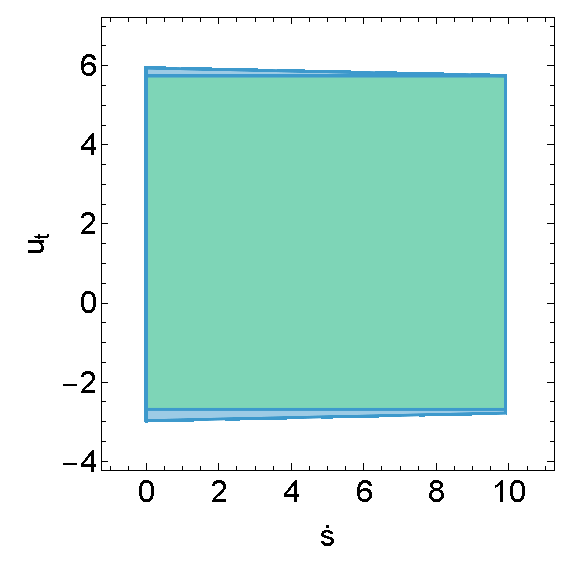
\includegraphics[width=\textwidth]{figures/inner_polytope/region_x3u1_plot_gr1.eps}
		\caption{Projection onto $\dot{s}$-$u_t$ plane}
	\end{subfigure}
	\begin{subfigure}[b]{0.32\textwidth}
		\centering
		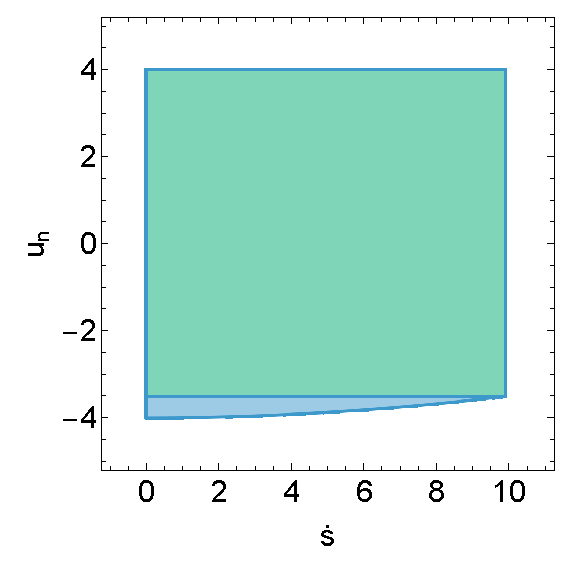
\includegraphics[width=\textwidth]{figures/inner_polytope/region_x3u2_plot_gr1.eps}
		\caption{Projection onto $\dot{s}$-$u_n$ plane}
	\end{subfigure}
	\begin{subfigure}[b]{0.32\textwidth}
		\centering
		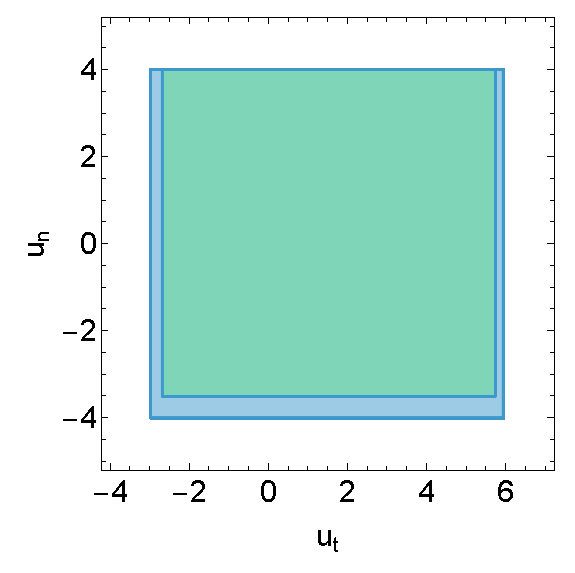
\includegraphics[width=\textwidth]{figures/inner_polytope/region_u1u2_plot_gr1.eps}
		\caption{Projection onto $u_t$-$u_n$ plane}
	\end{subfigure}
	\caption{In Green using Interval Fitting \ref{subsubsec:interval_fitting} and in Blue using CAD \ref{subsubsec:cad}.}
	\textbf{Parameters:} $C(s) \in \left[-\tfrac{1}{200},\, 0\right],\; s \in [0,\,10],\; n \in [0,\,2],\;$ \newline $v_x \in [0,\,10],\; v_y \in [-2,\,2],\; a_x \in [-3,\,6],\; a_y \in [-4,\,4],\;$ \newline $\dot{\psi} \in [-5,\,5],\; a_{\psi} \in [-2,\,2].$
	\label{fig:qe-comparison-with-params}
\end{figure}

Overall, while CAD can capture a more comprehensive feasible region, interval fitting (Approach~1) offers a compelling balance of computational
efficiency and practical accuracy, making it particularly well-suited for online or real-time motion planning.

\subsubsection{Limitations on Quantifier Elimination for Both Approaches}
\label{subsubsec:limitations_on_qe}

The general method of determining an inscribed polytope for Problem \ref{problem:inscribed_polytope} through quantifier elimination occurring in the
set \ref{eq:c_tilde} has certain limitations.

The approach tends to be conservative because the universal quantifier requires that all possible combinations of state variables must be feasible.
For instance, in a scenario with a long straight section immediately followed by a sharp left turn, the planner may enforce a single speed limit that
is valid for both segments, reducing maximum speed on the straight.
One way to mitigate this is by segmenting the road into smaller sections (e.g., splitting the straight from the turn) and defining distinct
constraint sets.
A higher-level switching mechanism can then determine when the vehicle transitions from one segment's constraints to the next.

Additionally, the initial intervals for $s$, $n$, and $\dot{n}$ in \eqref{eq:c_tilde} significantly impact the resulting feasible set.
To expand this set, the initial intervals for variables such as $\dot{s}$ and $\dot{n}$ can be chosen more precisely to reduce conservativeness.
We demonstrated this with a small nonlinear program (NLP) that treats the interval bounds as decision variables, guided by an objective function
(e.g., maximizing speed on straight segments).
As shown in Figure~\ref{fig:resulting_intervals_comparison}, a slight reduction in allowable longitudinal acceleration can result in a higher
feasible speed range, thus better utilizing the available road geometry.

\begin{figure}[h]
	\centering
	\begin{subfigure}[b]{0.45\textwidth}
		\centering
		\begin{align*}
			0    & \leq s \leq 10       \\
			0    & \leq n \leq 2        \\
			0    & \leq \dot{s} \leq 10 \\
			-2   & \leq \dot{n} \leq 2  \\
			-2.9 & \leq u_t \leq 5.9    \\
			-4   & \leq u_n \leq 3.75
		\end{align*}
		\caption{Initial Approach}
	\end{subfigure}
	\hfill
	\begin{subfigure}[b]{0.45\textwidth}
		\centering
		\begin{align*}
			0      & \leq s \leq 10,         \\
			0      & \leq n \leq 2,          \\
			0      & \leq \dot{s} \leq 10.05 \\
			-2     & \leq \dot{n} \leq 2     \\
			-2.899 & \leq u_t \leq 5.929     \\
			-4     & \leq u_n \leq 3.746
		\end{align*}
		\caption{Using Non-Linear Programming}
	\end{subfigure}
	\caption{Comparison of two sets of intervals for state variables and control inputs.}
	\label{fig:resulting_intervals_comparison}
\end{figure}

Overall, while these methods are highly effective for systematically constructing a feasible region under complex constraints, it is crucial to
mitigate over-conservativeness, particularly in dynamic driving scenarios where road geometry and speed limits vary significantly.

Next, we will introduce a transformation that maps the state variables and control inputs of the planning model to a steering angle, which can be
used to control a vehicle based on the equations from \cite{eilbrecht_challenges_2020}.
A similar approach is demonstrated in \cite{werling_optimal_2010}, which served as an additional inspiration.


\subsection{Determining the Steering Angle} \label{subsec:determining_the_steering_angle}

Typically, a vehicle is controlled through throttle, brakes, and a steering angle.
To incorporate these controls, we need to move away from visualizing our model as a box aligned with the road.
Instead, we will treat the model as a point and define its orientation based on its velocity.
We set $v_y = 0$ and $a_y=0$ to reflect that lateral motion arises solely from steering, thereby keeping the lateral velocity state zero and
capturing lateral movement through changes in heading rather than a separate lateral speed.
Using the equations \eqref{eq:first_derivative_long} and \eqref{eq:first_derivative_lat} with $v_y = 0$, we can solve for $v_x$.
\begin{equation}
	v := v_x = \sqrt{(1-nC(s))^2\dot{s}^2 + \dot{n}^2}
\end{equation}
Dividing $\dot{n}$ by $\dot{s}$ combined with  \eqref{eq:first_derivative_long} and \eqref{eq:first_derivative_lat} yields:
\begin{equation}
	\frac{\dot{n}}{\dot{s}} = (1-nC(s))\tan(\xi) = (1-nC(s))\tan(\psi - \theta)
\end{equation}
which we can solve for $\psi$ to get the orientation of the vehicle.
\begin{equation}
	\psi = \theta + \arctan\left(\frac{\dot{n}}{\dot{s}(1-nC(s))}\right)
\end{equation}

Using the state variables and $g$ from \eqref{def:g}, we can calculate $a_{x,tn}$ and $a_{y,tn}$ from \eqref{def:axtn} and \eqref{def:aytn},
respectively.
By substituting these values into equations \eqref{eq:second_derivative_long} and \eqref{eq:second_derivative_lat}, and setting $a_y = 0$, we can
determine the longitudinal acceleration and the change in orientation.
Additionally, we assume $|\xi| \leq \frac{\pi}{2}$ to ensure that $\cos{\xi} \neq 0$.
\begin{align}
	\dot{\psi} = \frac{a_{y,tn} - \tan(\xi) a_{x,tn}}{v (\tan(\xi) \sin(\xi) + \cos(\xi))} \\
	a := a_x = \frac{a_{x,tn} + v \dot{\psi} \sin(\xi)}{\cos{\xi}}
\end{align}
Our bicycle models \eqref{eq:dpsi_steering_angle} enables us to calculate the steering angle.
\begin{equation}
	\delta = \arctan(l_{wb}\frac{\dot{\psi}}{v})
\end{equation}
With those equations, we can define a transformation.
\begin{equation}
	T(\tilde{x}_{di}, \tilde{u}_{di}) = [p_x, p_y, \psi, \dot{\psi}, v, a, \delta] \label{eq:pm_state_transformation} \end{equation}

\subsection{Exact Discretization of the Double Integrator Model}

Using the simplified state and control representation from
Section~\ref{subsubsec:resulting_simplified_model}, the system dynamics \eqref{eq:pm_final_dynamics} are discretized using the matrix exponential
method \cite{kailath_linear_1980, ogata_modern_2010}.
The discrete-time system is formulated as:

\begin{equation}
	\label{eq:discrete_time_dynamics_di}
	\tilde{x}_{di, k+1} = A_d \tilde{x}_{di, k} + B_d \tilde{u}_{di, k} =: f_{d, di}(\tilde{x}_{di, k}, \tilde{u}_{di, k}, \Delta t),
\end{equation}

where the exact discretization is given by:

\begin{equation}
	A_d = e^{A \Delta t}, \quad B_d = \left( \int_0^{\Delta t} e^{A \tau} d\tau \right) B.
\end{equation}

Using the closed-form solution for the matrix exponential \cite{noauthor_matrix_nodate}, we obtain:

\begin{equation}
	A_d = \begin{bmatrix}
		1 & 0 & \Delta t & 0        \\
		0 & 1 & 0        & \Delta t \\
		0 & 0 & 1        & 0        \\
		0 & 0 & 0        & 1
	\end{bmatrix},
	\quad
	B_d = \begin{bmatrix}
		\frac{\Delta t^2}{2} & 0                    \\
		0                    & \frac{\Delta t^2}{2} \\
		\Delta t             & 0                    \\
		0                    & \Delta t
	\end{bmatrix}.
\end{equation}

This formulation ensures that the discrete-time representation accurately follows the continuous-time system over a sampling interval \( \Delta t \),
preserving dynamic consistency while enabling efficient convex optimization.
The resulting discrete-time model will be used in the subsequent trajectory planning formulation.

\subsection{Final Model Representation} \label{subsec:pm_resulting_model}

Our final model is represented by the following tuple.
\begin{equation}
	M_{pm} = (\tilde{x}_{di}, \tilde{u}_{di}, f_{d, di}, \hat{C}, T)
	\label{model:point_mass}
\end{equation}

\section{Motion Planning using Bicycle Model} \label{sec:motion_planning_using_bicylce}

We have already introduced the kinematic single track model in which a steering angle and an orientation, which will now combine with the idea of the
previous chapter.
We want to model our state variables in the road aligned frame, which is the Frenet frame.
The states and controls variables of the kinematic single track model are defined in the global coordinate system are defined as in \ref{eq:states_kst} and \ref{eq:controls_kst}:

\begin{figure}[h]
	\centering
	\begin{subfigure}[b]{0.45\textwidth}
		\centering
		$x = \begin{bmatrix} p_x \\ p_y \\ \delta \\ v \\ \psi \end{bmatrix}$
		\caption{State Variables}
	\end{subfigure}
	\hfill
	\begin{subfigure}[b]{0.45\textwidth}
		\centering
		$u = \begin{bmatrix} v_{\delta} \\ a_{\text{long}} \end{bmatrix}$
		\caption{Control Inputs}
	\end{subfigure}
\end{figure}

Our goal is not model dynamics and state variables in the Frenet frame.

\subsection{Transforming Global Cartesian Coordinates to Frenet Frame} \label{subsec:bicycle_conversion_of_cartesian_to_frenet}

In this section, we derive the state transition model for the Frenet frame, which is a commonly used coordinate system in vehicle dynamics and
control.
The Frenet frame is particularly useful for path tracking and motion planning as it simplifies the representation of the vehicle's motion relative to
a reference path.

We start by considering the dynamics of the kinematic single track model in the global coordinate system.
This model captures the essential behavior of a vehicle by representing it as a single point mass with a front and rear axle.
The state variables include the position coordinates $(p_x, p_y)$, the orientation angle $\psi$, the steering angle $\delta$, and the longitudinal
velocity $v$.
The control inputs are the longitudinal acceleration $a_{\text{long}}$ and the steering rate $v_{\delta}$.

The dynamics of the kinematic single track model in the global coordinate system are:

\begin{align*}
	 & \dot{p}_x = v\cos(\psi)                    \\
	 & \dot{p}_y = v\sin(\psi)                    \\
	 & \dot{\delta} = v_{\delta}                  \\
	 & \dot{v} = a_{\text{long}}                  \\
	 & \dot{\psi} = \frac{v}{l_{wb}} \tan(\delta) \\
\end{align*}

Building on the orientation model from the previous chapter, we can extend the point mass model to include body-fixed control inputs.
This approach helps us achieve our goal.

Using the previously derived equations \ref{eq:first_derivative_long} and \ref{eq:first_derivative_lat}, and incorporating the
definitions $\xi = \psi - \theta$ and $\dot{\theta}=\frac{d\theta}{ds}\frac{ds}{dt}=C(s)\dot{s}$, we obtain
the following equations:

\begin{align*}
	\dot{s} = \frac{v_x\cos{\xi}}{1-nC(s)} \\
	\dot{n} = v_x\sin{\xi}                 \\
	\dot{\xi} = \dot{\psi} - C(s)\dot{s}   \\
\end{align*}

Combining these equations with the kinematic single track model, we derive the state transition model for the Frenet frame.
This model provides a comprehensive representation of the vehicle's motion in the Frenet coordinate system, which is essential for accurate path
tracking and motion planning.

Next, we define the state variables and control inputs for the single-track model.

\subsection{Model Dynamics Approximation} \label{subsec:approximation_of_model_dynamics}

The state variables and control inputs for the single-track model in the Frenet frame are defined as follows:
\begin{figure}[h]
	\centering
	\begin{subfigure}[b]{0.45\textwidth}
		\centering
		$x = \begin{bmatrix}
				s \\ n \\ \xi \\ v \\ \delta
			\end{bmatrix}$
		\caption{State Variables}
	\end{subfigure}
	\hfill
	\begin{subfigure}[b]{0.45\textwidth}
		\centering
		$u = \begin{bmatrix}
				a_{x,b} \\ v_\delta
			\end{bmatrix}$
		\caption{Control Inputs}
	\end{subfigure}
\end{figure}

where the state consists of the Frenet frame coordinates $(s, n)$, the heading alignment error $\xi$, the longitudinal vehicle velocity $v$, and the steering angle $\delta$.
The state evolution is described by the following equations:

\begin{equation}
	f(x, u) =
	\begin{bmatrix}
		\frac{v \cos\xi}{1 - nC(s)}                \\[8pt]
		v \sin\xi                                  \\[8pt]
		\frac{1}{l_{wb}}v \tan\delta - C(s)\dot{s} \\[8pt]
		a_{x,b}                                    \\[8pt]
		v_\delta
	\end{bmatrix}.
\end{equation}

For this model, we will use body-fixed control inputs, which provide convex road topology constraints.
To linearize the model dynamics, we will use two new techniques.
These techniques allow us to maintain the constraints without shifting, as was necessary in the previous chapter.
This ensures a more accurate and computationally efficient representation of the vehicle's motion.

To simplify the model, the following assumptions are made: $nC(s)$ is close to zero.
This is a valid since $n$ models the vehicle's lateral position relative to the reference path, and $C(s)$ is the curvature of the reference path
which is typically small enough for this assumption to be valid.
We split up the problem by looking the terms which make the model non-linear.

\subsubsection{Non-Linear Terms}

We have four non-linear terms in the state transition model.
In the following, we linearize them using approximations.
\begin{align}
	 & \frac{v \cos\xi}{1 - nC(s)} \\
	 & v \sin\xi                   \\
	 & v \tan\delta                \\
	 & C(s)\dot{s}
\end{align}

With our assumptions, that $nC(s)\approx 0$, we can immediately simplify the first term.

\[
	\frac{v \cos\xi}{1 - nC(s)} \approx v \cos\xi
\]

\subsubsection{First Order Taylor Polynomial}

To linearize the non-linear terms, we use the first order Taylor polynomial approximation around a reference point.
The first order Taylor expansion of a function \(f(x)\) around a point \(x_0\) is given by:

\[ f(x) \approx f(x_0) +
	\frac{df}{dx} (x_0) (x - x_0) \]

Applying the first order Taylor polynomial to the trigonometric functions $\sin$, $\cos$, and
$\tan$ around the reference points $\xi_0$ and $\delta_0$, we obtain the following approximations:

\[ \cos(\xi) \approx
	\cos(\xi_0) - \sin(\xi_0) (\xi - \xi_0) \] \[ \sin(\xi) \approx \sin(\xi_0) + \cos(\xi_0) (\xi - \xi_0) \] \[ \tan(\delta) \approx \tan(\delta_0) +
	\frac{1}{\cos^2(\delta_0)} (\delta - \delta_0) \]

These approximations are known as small angle approximations, which are valid
when the angles $\xi$ and $\delta$ are small.
In vehicle dynamics, it is often reasonable to assume that the heading alignment error $\xi$ and the steering angle $\delta$ are small, especially
when the vehicle is closely following a reference path.
This allows us to simplify the trigonometric functions using their first order Taylor expansions.

Substituting these first order Taylor approximations into the state transition model, we obtain the following terms:

\begin{align*}
	 & v (\cos(\xi_0) - \sin(\xi_0) (\xi - \xi_0))                         \\
	 & v (\sin(\xi_0) + \cos(\xi_0) (\xi - \xi_0))                         \\
	 & v (\tan(\delta_0) + \frac{1}{\cos^2(\delta_0)} (\delta - \delta_0)) \\
	 & C(s)\dot{s}
\end{align*}

Since our reference values $\xi_0 = 0$ and $\delta_0 = 0$ are constant the only remaining non-linear terms are: $$v \xi, v \delta, C(s)\dot{s}$$

Bilinear terms arise when the product of two variables appears in the equations, making the system non-linear.
In our state transition model, the terms \(v \xi\), \(v \delta\), and \(C(s)\dot{s}\) are bilinear.
Since \(C(s)\) is a function of \(s\), we will introduce another assumption.
We have already seen that we can model our road in segments, which we used for the Point Mass Model to obtain less conservative coupling constraints.
Here, we will reuse this approach to linearize our dynamics.

\subsubsection{Assumption: Piece Wise Linear Curvature}

We assume that the curvature can be expressed as a piece-wise linear function.

\[
	C(s) = \begin{cases}
		a_1s+b_1 & \text{if } s \in [s_0, s_1]     \\
		a_2s+b_2 & \text{if } s \in [s_1, s_2]     \\
		\vdots                                     \\
		a_ns+b_n & \text{if } s \in [s_{n-1}, s_n]
	\end{cases}
\]

This reduces the non-linear term \(C(s)\dot{s}\) to a new bilinear term \(s\dot{s}\), which we need to linearize.

Next, we will focus on linearizing the bilinear terms.

\subsection{Convex Relaxation of Bilinear Terms} \label{subsec:convex_relaxation_for_bilinear_terms}

To handle bilinear terms of the form \(xy\), we introduce a new variable \(w\) and apply the McCormick relaxation.
The McCormick relaxation is a technique that linearizes bilinear terms by introducing auxiliary variables and constraints.
This technique allows us to represent the bilinear terms as a set of linear constraints, which can be solved efficiently using convex optimization
methods.
This relaxation only works if the variables \(x\) and \(y\) are bounded:

\[ \underline{x} \leq x \leq \overline{x}, \qquad
	\underline{y} \leq y \leq \overline{y} \] with constants \(\underline{x}, \overline{x}, \underline{y}, \overline{y} \in \mathbb{R}\).

We introduce a new auxiliary variable \(w\), which will be used as an approximation of the bilinear term \(xy\).
We use linear constraints to bound the auxiliary variable \(w\) and ensure that it approximates the bilinear term \(xy\).
The linear constraints are derived from the bounds of the variables \(x\), \(y\), and the bilinear term \(xy\), as shown below:

\[
	\begin{aligned}
		w & \geq \underline{x} y + x \underline{y} - \underline{x} \underline{y}, \\
		w & \geq \overline{x} y + x \overline{y} - \overline{x} \overline{y},     \\
		w & \leq \overline{x} y + x \underline{y} - \overline{x} \underline{y},   \\
		w & \leq \underline{x} y + x \overline{y} - \underline{x} \overline{y}.
	\end{aligned}
\]

The idea behind these constraints is to create a convex lower bound and a concave upper bound for the bilinear term \(xy\).
These bounds are constructed as follows: \[ a = (x - \underline{x}) \geq 0 \] \[ b = (y - \underline{y}) \geq 0 \] Since a and b are both positive,
we can multiply them to get: \[ ab = xy - \underline{x}y - \underline{y}x + \underline{x}\underline{y} \geq 0 \] Thus, we get our first under
estimator for $xy$: \[ xy \geq \underline{x}y + \underline{y}x - \underline{x}\underline{y} \] To get the all the possible lower and upper bounds by
what is given we can apply this pattern to $a\in\{x - \underline{x}, \overline{x} - x\}$ and $b\in\{y - \underline{y}, \overline{y} - y\}$.
For any of the four possible combination of $a$ and $b$ we get $ab\geq0$ and can therefor come up with either an upper or lower bound for $xy$.

\begin{figure}[h]
	\centering
	\begin{subfigure}[b]{0.45\textwidth}
		\centering
		\resizebox{\textwidth}{!}{%% Creator: Matplotlib, PGF backend
%%
%% To include the figure in your LaTeX document, write
%%   \input{<filename>.pgf}
%%
%% Make sure the required packages are loaded in your preamble
%%   \usepackage{pgf}
%%
%% Also ensure that all the required font packages are loaded; for instance,
%% the lmodern package is sometimes necessary when using math font.
%%   \usepackage{lmodern}
%%
%% Figures using additional raster images can only be included by \input if
%% they are in the same directory as the main LaTeX file. For loading figures
%% from other directories you can use the `import` package
%%   \usepackage{import}
%%
%% and then include the figures with
%%   \import{<path to file>}{<filename>.pgf}
%%
%% Matplotlib used the following preamble
%%   \def\mathdefault#1{#1}
%%   \everymath=\expandafter{\the\everymath\displaystyle}
%%   
%%   \ifdefined\pdftexversion\else  % non-pdftex case.
%%     \usepackage{fontspec}
%%   \fi
%%   \makeatletter\@ifpackageloaded{underscore}{}{\usepackage[strings]{underscore}}\makeatother
%%
\begingroup%
\makeatletter%
\begin{pgfpicture}%
\pgfpathrectangle{\pgfpointorigin}{\pgfqpoint{4.377484in}{3.839102in}}%
\pgfusepath{use as bounding box, clip}%
\begin{pgfscope}%
\pgfsetbuttcap%
\pgfsetmiterjoin%
\definecolor{currentfill}{rgb}{1.000000,1.000000,1.000000}%
\pgfsetfillcolor{currentfill}%
\pgfsetlinewidth{0.000000pt}%
\definecolor{currentstroke}{rgb}{1.000000,1.000000,1.000000}%
\pgfsetstrokecolor{currentstroke}%
\pgfsetdash{}{0pt}%
\pgfpathmoveto{\pgfqpoint{0.000000in}{0.000000in}}%
\pgfpathlineto{\pgfqpoint{4.377484in}{0.000000in}}%
\pgfpathlineto{\pgfqpoint{4.377484in}{3.839102in}}%
\pgfpathlineto{\pgfqpoint{0.000000in}{3.839102in}}%
\pgfpathlineto{\pgfqpoint{0.000000in}{0.000000in}}%
\pgfpathclose%
\pgfusepath{fill}%
\end{pgfscope}%
\begin{pgfscope}%
\pgfsetbuttcap%
\pgfsetmiterjoin%
\definecolor{currentfill}{rgb}{1.000000,1.000000,1.000000}%
\pgfsetfillcolor{currentfill}%
\pgfsetlinewidth{0.000000pt}%
\definecolor{currentstroke}{rgb}{0.000000,0.000000,0.000000}%
\pgfsetstrokecolor{currentstroke}%
\pgfsetstrokeopacity{0.000000}%
\pgfsetdash{}{0pt}%
\pgfpathmoveto{\pgfqpoint{0.516434in}{0.499074in}}%
\pgfpathlineto{\pgfqpoint{3.713060in}{0.499074in}}%
\pgfpathlineto{\pgfqpoint{3.713060in}{3.695699in}}%
\pgfpathlineto{\pgfqpoint{0.516434in}{3.695699in}}%
\pgfpathlineto{\pgfqpoint{0.516434in}{0.499074in}}%
\pgfpathclose%
\pgfusepath{fill}%
\end{pgfscope}%
\begin{pgfscope}%
\pgfpathrectangle{\pgfqpoint{0.516434in}{0.499074in}}{\pgfqpoint{3.196625in}{3.196625in}}%
\pgfusepath{clip}%
\pgfsys@transformshift{0.516434in}{0.499074in}%
\pgftext[left,bottom]{
\includegraphics[interpolate=true,width=3.200000in,height=3.200000in]{figures/mccormick/mccormick-bounds-0-upper-img0.png}}%
\end{pgfscope}%
\begin{pgfscope}%
\pgfsetbuttcap%
\pgfsetroundjoin%
\definecolor{currentfill}{rgb}{0.000000,0.000000,0.000000}%
\pgfsetfillcolor{currentfill}%
\pgfsetlinewidth{0.803000pt}%
\definecolor{currentstroke}{rgb}{0.000000,0.000000,0.000000}%
\pgfsetstrokecolor{currentstroke}%
\pgfsetdash{}{0pt}%
\pgfsys@defobject{currentmarker}{\pgfqpoint{0.000000in}{-0.048611in}}{\pgfqpoint{0.000000in}{0.000000in}}{%
\pgfpathmoveto{\pgfqpoint{0.000000in}{0.000000in}}%
\pgfpathlineto{\pgfqpoint{0.000000in}{-0.048611in}}%
\pgfusepath{stroke,fill}%
}%
\begin{pgfscope}%
\pgfsys@transformshift{0.516434in}{0.499074in}%
\pgfsys@useobject{currentmarker}{}%
\end{pgfscope}%
\end{pgfscope}%
\begin{pgfscope}%
\definecolor{textcolor}{rgb}{0.000000,0.000000,0.000000}%
\pgfsetstrokecolor{textcolor}%
\pgfsetfillcolor{textcolor}%
\pgftext[x=0.516434in,y=0.401852in,,top]{\color{textcolor}{\rmfamily\fontsize{9.000000}{10.800000}\selectfont\catcode`\^=\active\def^{\ifmmode\sp\else\^{}\fi}\catcode`\%=\active\def%{\%}$\mathdefault{\ensuremath{-}2.0}$}}%
\end{pgfscope}%
\begin{pgfscope}%
\pgfsetbuttcap%
\pgfsetroundjoin%
\definecolor{currentfill}{rgb}{0.000000,0.000000,0.000000}%
\pgfsetfillcolor{currentfill}%
\pgfsetlinewidth{0.803000pt}%
\definecolor{currentstroke}{rgb}{0.000000,0.000000,0.000000}%
\pgfsetstrokecolor{currentstroke}%
\pgfsetdash{}{0pt}%
\pgfsys@defobject{currentmarker}{\pgfqpoint{0.000000in}{-0.048611in}}{\pgfqpoint{0.000000in}{0.000000in}}{%
\pgfpathmoveto{\pgfqpoint{0.000000in}{0.000000in}}%
\pgfpathlineto{\pgfqpoint{0.000000in}{-0.048611in}}%
\pgfusepath{stroke,fill}%
}%
\begin{pgfscope}%
\pgfsys@transformshift{0.916012in}{0.499074in}%
\pgfsys@useobject{currentmarker}{}%
\end{pgfscope}%
\end{pgfscope}%
\begin{pgfscope}%
\definecolor{textcolor}{rgb}{0.000000,0.000000,0.000000}%
\pgfsetstrokecolor{textcolor}%
\pgfsetfillcolor{textcolor}%
\pgftext[x=0.916012in,y=0.401852in,,top]{\color{textcolor}{\rmfamily\fontsize{9.000000}{10.800000}\selectfont\catcode`\^=\active\def^{\ifmmode\sp\else\^{}\fi}\catcode`\%=\active\def%{\%}$\mathdefault{\ensuremath{-}1.5}$}}%
\end{pgfscope}%
\begin{pgfscope}%
\pgfsetbuttcap%
\pgfsetroundjoin%
\definecolor{currentfill}{rgb}{0.000000,0.000000,0.000000}%
\pgfsetfillcolor{currentfill}%
\pgfsetlinewidth{0.803000pt}%
\definecolor{currentstroke}{rgb}{0.000000,0.000000,0.000000}%
\pgfsetstrokecolor{currentstroke}%
\pgfsetdash{}{0pt}%
\pgfsys@defobject{currentmarker}{\pgfqpoint{0.000000in}{-0.048611in}}{\pgfqpoint{0.000000in}{0.000000in}}{%
\pgfpathmoveto{\pgfqpoint{0.000000in}{0.000000in}}%
\pgfpathlineto{\pgfqpoint{0.000000in}{-0.048611in}}%
\pgfusepath{stroke,fill}%
}%
\begin{pgfscope}%
\pgfsys@transformshift{1.315591in}{0.499074in}%
\pgfsys@useobject{currentmarker}{}%
\end{pgfscope}%
\end{pgfscope}%
\begin{pgfscope}%
\definecolor{textcolor}{rgb}{0.000000,0.000000,0.000000}%
\pgfsetstrokecolor{textcolor}%
\pgfsetfillcolor{textcolor}%
\pgftext[x=1.315591in,y=0.401852in,,top]{\color{textcolor}{\rmfamily\fontsize{9.000000}{10.800000}\selectfont\catcode`\^=\active\def^{\ifmmode\sp\else\^{}\fi}\catcode`\%=\active\def%{\%}$\mathdefault{\ensuremath{-}1.0}$}}%
\end{pgfscope}%
\begin{pgfscope}%
\pgfsetbuttcap%
\pgfsetroundjoin%
\definecolor{currentfill}{rgb}{0.000000,0.000000,0.000000}%
\pgfsetfillcolor{currentfill}%
\pgfsetlinewidth{0.803000pt}%
\definecolor{currentstroke}{rgb}{0.000000,0.000000,0.000000}%
\pgfsetstrokecolor{currentstroke}%
\pgfsetdash{}{0pt}%
\pgfsys@defobject{currentmarker}{\pgfqpoint{0.000000in}{-0.048611in}}{\pgfqpoint{0.000000in}{0.000000in}}{%
\pgfpathmoveto{\pgfqpoint{0.000000in}{0.000000in}}%
\pgfpathlineto{\pgfqpoint{0.000000in}{-0.048611in}}%
\pgfusepath{stroke,fill}%
}%
\begin{pgfscope}%
\pgfsys@transformshift{1.715169in}{0.499074in}%
\pgfsys@useobject{currentmarker}{}%
\end{pgfscope}%
\end{pgfscope}%
\begin{pgfscope}%
\definecolor{textcolor}{rgb}{0.000000,0.000000,0.000000}%
\pgfsetstrokecolor{textcolor}%
\pgfsetfillcolor{textcolor}%
\pgftext[x=1.715169in,y=0.401852in,,top]{\color{textcolor}{\rmfamily\fontsize{9.000000}{10.800000}\selectfont\catcode`\^=\active\def^{\ifmmode\sp\else\^{}\fi}\catcode`\%=\active\def%{\%}$\mathdefault{\ensuremath{-}0.5}$}}%
\end{pgfscope}%
\begin{pgfscope}%
\pgfsetbuttcap%
\pgfsetroundjoin%
\definecolor{currentfill}{rgb}{0.000000,0.000000,0.000000}%
\pgfsetfillcolor{currentfill}%
\pgfsetlinewidth{0.803000pt}%
\definecolor{currentstroke}{rgb}{0.000000,0.000000,0.000000}%
\pgfsetstrokecolor{currentstroke}%
\pgfsetdash{}{0pt}%
\pgfsys@defobject{currentmarker}{\pgfqpoint{0.000000in}{-0.048611in}}{\pgfqpoint{0.000000in}{0.000000in}}{%
\pgfpathmoveto{\pgfqpoint{0.000000in}{0.000000in}}%
\pgfpathlineto{\pgfqpoint{0.000000in}{-0.048611in}}%
\pgfusepath{stroke,fill}%
}%
\begin{pgfscope}%
\pgfsys@transformshift{2.114747in}{0.499074in}%
\pgfsys@useobject{currentmarker}{}%
\end{pgfscope}%
\end{pgfscope}%
\begin{pgfscope}%
\definecolor{textcolor}{rgb}{0.000000,0.000000,0.000000}%
\pgfsetstrokecolor{textcolor}%
\pgfsetfillcolor{textcolor}%
\pgftext[x=2.114747in,y=0.401852in,,top]{\color{textcolor}{\rmfamily\fontsize{9.000000}{10.800000}\selectfont\catcode`\^=\active\def^{\ifmmode\sp\else\^{}\fi}\catcode`\%=\active\def%{\%}$\mathdefault{0.0}$}}%
\end{pgfscope}%
\begin{pgfscope}%
\pgfsetbuttcap%
\pgfsetroundjoin%
\definecolor{currentfill}{rgb}{0.000000,0.000000,0.000000}%
\pgfsetfillcolor{currentfill}%
\pgfsetlinewidth{0.803000pt}%
\definecolor{currentstroke}{rgb}{0.000000,0.000000,0.000000}%
\pgfsetstrokecolor{currentstroke}%
\pgfsetdash{}{0pt}%
\pgfsys@defobject{currentmarker}{\pgfqpoint{0.000000in}{-0.048611in}}{\pgfqpoint{0.000000in}{0.000000in}}{%
\pgfpathmoveto{\pgfqpoint{0.000000in}{0.000000in}}%
\pgfpathlineto{\pgfqpoint{0.000000in}{-0.048611in}}%
\pgfusepath{stroke,fill}%
}%
\begin{pgfscope}%
\pgfsys@transformshift{2.514325in}{0.499074in}%
\pgfsys@useobject{currentmarker}{}%
\end{pgfscope}%
\end{pgfscope}%
\begin{pgfscope}%
\definecolor{textcolor}{rgb}{0.000000,0.000000,0.000000}%
\pgfsetstrokecolor{textcolor}%
\pgfsetfillcolor{textcolor}%
\pgftext[x=2.514325in,y=0.401852in,,top]{\color{textcolor}{\rmfamily\fontsize{9.000000}{10.800000}\selectfont\catcode`\^=\active\def^{\ifmmode\sp\else\^{}\fi}\catcode`\%=\active\def%{\%}$\mathdefault{0.5}$}}%
\end{pgfscope}%
\begin{pgfscope}%
\pgfsetbuttcap%
\pgfsetroundjoin%
\definecolor{currentfill}{rgb}{0.000000,0.000000,0.000000}%
\pgfsetfillcolor{currentfill}%
\pgfsetlinewidth{0.803000pt}%
\definecolor{currentstroke}{rgb}{0.000000,0.000000,0.000000}%
\pgfsetstrokecolor{currentstroke}%
\pgfsetdash{}{0pt}%
\pgfsys@defobject{currentmarker}{\pgfqpoint{0.000000in}{-0.048611in}}{\pgfqpoint{0.000000in}{0.000000in}}{%
\pgfpathmoveto{\pgfqpoint{0.000000in}{0.000000in}}%
\pgfpathlineto{\pgfqpoint{0.000000in}{-0.048611in}}%
\pgfusepath{stroke,fill}%
}%
\begin{pgfscope}%
\pgfsys@transformshift{2.913903in}{0.499074in}%
\pgfsys@useobject{currentmarker}{}%
\end{pgfscope}%
\end{pgfscope}%
\begin{pgfscope}%
\definecolor{textcolor}{rgb}{0.000000,0.000000,0.000000}%
\pgfsetstrokecolor{textcolor}%
\pgfsetfillcolor{textcolor}%
\pgftext[x=2.913903in,y=0.401852in,,top]{\color{textcolor}{\rmfamily\fontsize{9.000000}{10.800000}\selectfont\catcode`\^=\active\def^{\ifmmode\sp\else\^{}\fi}\catcode`\%=\active\def%{\%}$\mathdefault{1.0}$}}%
\end{pgfscope}%
\begin{pgfscope}%
\pgfsetbuttcap%
\pgfsetroundjoin%
\definecolor{currentfill}{rgb}{0.000000,0.000000,0.000000}%
\pgfsetfillcolor{currentfill}%
\pgfsetlinewidth{0.803000pt}%
\definecolor{currentstroke}{rgb}{0.000000,0.000000,0.000000}%
\pgfsetstrokecolor{currentstroke}%
\pgfsetdash{}{0pt}%
\pgfsys@defobject{currentmarker}{\pgfqpoint{0.000000in}{-0.048611in}}{\pgfqpoint{0.000000in}{0.000000in}}{%
\pgfpathmoveto{\pgfqpoint{0.000000in}{0.000000in}}%
\pgfpathlineto{\pgfqpoint{0.000000in}{-0.048611in}}%
\pgfusepath{stroke,fill}%
}%
\begin{pgfscope}%
\pgfsys@transformshift{3.313482in}{0.499074in}%
\pgfsys@useobject{currentmarker}{}%
\end{pgfscope}%
\end{pgfscope}%
\begin{pgfscope}%
\definecolor{textcolor}{rgb}{0.000000,0.000000,0.000000}%
\pgfsetstrokecolor{textcolor}%
\pgfsetfillcolor{textcolor}%
\pgftext[x=3.313482in,y=0.401852in,,top]{\color{textcolor}{\rmfamily\fontsize{9.000000}{10.800000}\selectfont\catcode`\^=\active\def^{\ifmmode\sp\else\^{}\fi}\catcode`\%=\active\def%{\%}$\mathdefault{1.5}$}}%
\end{pgfscope}%
\begin{pgfscope}%
\pgfsetbuttcap%
\pgfsetroundjoin%
\definecolor{currentfill}{rgb}{0.000000,0.000000,0.000000}%
\pgfsetfillcolor{currentfill}%
\pgfsetlinewidth{0.803000pt}%
\definecolor{currentstroke}{rgb}{0.000000,0.000000,0.000000}%
\pgfsetstrokecolor{currentstroke}%
\pgfsetdash{}{0pt}%
\pgfsys@defobject{currentmarker}{\pgfqpoint{0.000000in}{-0.048611in}}{\pgfqpoint{0.000000in}{0.000000in}}{%
\pgfpathmoveto{\pgfqpoint{0.000000in}{0.000000in}}%
\pgfpathlineto{\pgfqpoint{0.000000in}{-0.048611in}}%
\pgfusepath{stroke,fill}%
}%
\begin{pgfscope}%
\pgfsys@transformshift{3.713060in}{0.499074in}%
\pgfsys@useobject{currentmarker}{}%
\end{pgfscope}%
\end{pgfscope}%
\begin{pgfscope}%
\definecolor{textcolor}{rgb}{0.000000,0.000000,0.000000}%
\pgfsetstrokecolor{textcolor}%
\pgfsetfillcolor{textcolor}%
\pgftext[x=3.713060in,y=0.401852in,,top]{\color{textcolor}{\rmfamily\fontsize{9.000000}{10.800000}\selectfont\catcode`\^=\active\def^{\ifmmode\sp\else\^{}\fi}\catcode`\%=\active\def%{\%}$\mathdefault{2.0}$}}%
\end{pgfscope}%
\begin{pgfscope}%
\definecolor{textcolor}{rgb}{0.000000,0.000000,0.000000}%
\pgfsetstrokecolor{textcolor}%
\pgfsetfillcolor{textcolor}%
\pgftext[x=2.114747in,y=0.235185in,,top]{\color{textcolor}{\rmfamily\fontsize{11.000000}{13.200000}\selectfont\catcode`\^=\active\def^{\ifmmode\sp\else\^{}\fi}\catcode`\%=\active\def%{\%}$v_1$}}%
\end{pgfscope}%
\begin{pgfscope}%
\pgfsetbuttcap%
\pgfsetroundjoin%
\definecolor{currentfill}{rgb}{0.000000,0.000000,0.000000}%
\pgfsetfillcolor{currentfill}%
\pgfsetlinewidth{0.803000pt}%
\definecolor{currentstroke}{rgb}{0.000000,0.000000,0.000000}%
\pgfsetstrokecolor{currentstroke}%
\pgfsetdash{}{0pt}%
\pgfsys@defobject{currentmarker}{\pgfqpoint{-0.048611in}{0.000000in}}{\pgfqpoint{-0.000000in}{0.000000in}}{%
\pgfpathmoveto{\pgfqpoint{-0.000000in}{0.000000in}}%
\pgfpathlineto{\pgfqpoint{-0.048611in}{0.000000in}}%
\pgfusepath{stroke,fill}%
}%
\begin{pgfscope}%
\pgfsys@transformshift{0.516434in}{0.499074in}%
\pgfsys@useobject{currentmarker}{}%
\end{pgfscope}%
\end{pgfscope}%
\begin{pgfscope}%
\definecolor{textcolor}{rgb}{0.000000,0.000000,0.000000}%
\pgfsetstrokecolor{textcolor}%
\pgfsetfillcolor{textcolor}%
\pgftext[x=0.354976in, y=0.455671in, left, base]{\color{textcolor}{\rmfamily\fontsize{9.000000}{10.800000}\selectfont\catcode`\^=\active\def^{\ifmmode\sp\else\^{}\fi}\catcode`\%=\active\def%{\%}$\mathdefault{0}$}}%
\end{pgfscope}%
\begin{pgfscope}%
\pgfsetbuttcap%
\pgfsetroundjoin%
\definecolor{currentfill}{rgb}{0.000000,0.000000,0.000000}%
\pgfsetfillcolor{currentfill}%
\pgfsetlinewidth{0.803000pt}%
\definecolor{currentstroke}{rgb}{0.000000,0.000000,0.000000}%
\pgfsetstrokecolor{currentstroke}%
\pgfsetdash{}{0pt}%
\pgfsys@defobject{currentmarker}{\pgfqpoint{-0.048611in}{0.000000in}}{\pgfqpoint{-0.000000in}{0.000000in}}{%
\pgfpathmoveto{\pgfqpoint{-0.000000in}{0.000000in}}%
\pgfpathlineto{\pgfqpoint{-0.048611in}{0.000000in}}%
\pgfusepath{stroke,fill}%
}%
\begin{pgfscope}%
\pgfsys@transformshift{0.516434in}{1.138399in}%
\pgfsys@useobject{currentmarker}{}%
\end{pgfscope}%
\end{pgfscope}%
\begin{pgfscope}%
\definecolor{textcolor}{rgb}{0.000000,0.000000,0.000000}%
\pgfsetstrokecolor{textcolor}%
\pgfsetfillcolor{textcolor}%
\pgftext[x=0.290741in, y=1.094996in, left, base]{\color{textcolor}{\rmfamily\fontsize{9.000000}{10.800000}\selectfont\catcode`\^=\active\def^{\ifmmode\sp\else\^{}\fi}\catcode`\%=\active\def%{\%}$\mathdefault{10}$}}%
\end{pgfscope}%
\begin{pgfscope}%
\pgfsetbuttcap%
\pgfsetroundjoin%
\definecolor{currentfill}{rgb}{0.000000,0.000000,0.000000}%
\pgfsetfillcolor{currentfill}%
\pgfsetlinewidth{0.803000pt}%
\definecolor{currentstroke}{rgb}{0.000000,0.000000,0.000000}%
\pgfsetstrokecolor{currentstroke}%
\pgfsetdash{}{0pt}%
\pgfsys@defobject{currentmarker}{\pgfqpoint{-0.048611in}{0.000000in}}{\pgfqpoint{-0.000000in}{0.000000in}}{%
\pgfpathmoveto{\pgfqpoint{-0.000000in}{0.000000in}}%
\pgfpathlineto{\pgfqpoint{-0.048611in}{0.000000in}}%
\pgfusepath{stroke,fill}%
}%
\begin{pgfscope}%
\pgfsys@transformshift{0.516434in}{1.777724in}%
\pgfsys@useobject{currentmarker}{}%
\end{pgfscope}%
\end{pgfscope}%
\begin{pgfscope}%
\definecolor{textcolor}{rgb}{0.000000,0.000000,0.000000}%
\pgfsetstrokecolor{textcolor}%
\pgfsetfillcolor{textcolor}%
\pgftext[x=0.290741in, y=1.734321in, left, base]{\color{textcolor}{\rmfamily\fontsize{9.000000}{10.800000}\selectfont\catcode`\^=\active\def^{\ifmmode\sp\else\^{}\fi}\catcode`\%=\active\def%{\%}$\mathdefault{20}$}}%
\end{pgfscope}%
\begin{pgfscope}%
\pgfsetbuttcap%
\pgfsetroundjoin%
\definecolor{currentfill}{rgb}{0.000000,0.000000,0.000000}%
\pgfsetfillcolor{currentfill}%
\pgfsetlinewidth{0.803000pt}%
\definecolor{currentstroke}{rgb}{0.000000,0.000000,0.000000}%
\pgfsetstrokecolor{currentstroke}%
\pgfsetdash{}{0pt}%
\pgfsys@defobject{currentmarker}{\pgfqpoint{-0.048611in}{0.000000in}}{\pgfqpoint{-0.000000in}{0.000000in}}{%
\pgfpathmoveto{\pgfqpoint{-0.000000in}{0.000000in}}%
\pgfpathlineto{\pgfqpoint{-0.048611in}{0.000000in}}%
\pgfusepath{stroke,fill}%
}%
\begin{pgfscope}%
\pgfsys@transformshift{0.516434in}{2.417049in}%
\pgfsys@useobject{currentmarker}{}%
\end{pgfscope}%
\end{pgfscope}%
\begin{pgfscope}%
\definecolor{textcolor}{rgb}{0.000000,0.000000,0.000000}%
\pgfsetstrokecolor{textcolor}%
\pgfsetfillcolor{textcolor}%
\pgftext[x=0.290741in, y=2.373646in, left, base]{\color{textcolor}{\rmfamily\fontsize{9.000000}{10.800000}\selectfont\catcode`\^=\active\def^{\ifmmode\sp\else\^{}\fi}\catcode`\%=\active\def%{\%}$\mathdefault{30}$}}%
\end{pgfscope}%
\begin{pgfscope}%
\pgfsetbuttcap%
\pgfsetroundjoin%
\definecolor{currentfill}{rgb}{0.000000,0.000000,0.000000}%
\pgfsetfillcolor{currentfill}%
\pgfsetlinewidth{0.803000pt}%
\definecolor{currentstroke}{rgb}{0.000000,0.000000,0.000000}%
\pgfsetstrokecolor{currentstroke}%
\pgfsetdash{}{0pt}%
\pgfsys@defobject{currentmarker}{\pgfqpoint{-0.048611in}{0.000000in}}{\pgfqpoint{-0.000000in}{0.000000in}}{%
\pgfpathmoveto{\pgfqpoint{-0.000000in}{0.000000in}}%
\pgfpathlineto{\pgfqpoint{-0.048611in}{0.000000in}}%
\pgfusepath{stroke,fill}%
}%
\begin{pgfscope}%
\pgfsys@transformshift{0.516434in}{3.056374in}%
\pgfsys@useobject{currentmarker}{}%
\end{pgfscope}%
\end{pgfscope}%
\begin{pgfscope}%
\definecolor{textcolor}{rgb}{0.000000,0.000000,0.000000}%
\pgfsetstrokecolor{textcolor}%
\pgfsetfillcolor{textcolor}%
\pgftext[x=0.290741in, y=3.012972in, left, base]{\color{textcolor}{\rmfamily\fontsize{9.000000}{10.800000}\selectfont\catcode`\^=\active\def^{\ifmmode\sp\else\^{}\fi}\catcode`\%=\active\def%{\%}$\mathdefault{40}$}}%
\end{pgfscope}%
\begin{pgfscope}%
\pgfsetbuttcap%
\pgfsetroundjoin%
\definecolor{currentfill}{rgb}{0.000000,0.000000,0.000000}%
\pgfsetfillcolor{currentfill}%
\pgfsetlinewidth{0.803000pt}%
\definecolor{currentstroke}{rgb}{0.000000,0.000000,0.000000}%
\pgfsetstrokecolor{currentstroke}%
\pgfsetdash{}{0pt}%
\pgfsys@defobject{currentmarker}{\pgfqpoint{-0.048611in}{0.000000in}}{\pgfqpoint{-0.000000in}{0.000000in}}{%
\pgfpathmoveto{\pgfqpoint{-0.000000in}{0.000000in}}%
\pgfpathlineto{\pgfqpoint{-0.048611in}{0.000000in}}%
\pgfusepath{stroke,fill}%
}%
\begin{pgfscope}%
\pgfsys@transformshift{0.516434in}{3.695699in}%
\pgfsys@useobject{currentmarker}{}%
\end{pgfscope}%
\end{pgfscope}%
\begin{pgfscope}%
\definecolor{textcolor}{rgb}{0.000000,0.000000,0.000000}%
\pgfsetstrokecolor{textcolor}%
\pgfsetfillcolor{textcolor}%
\pgftext[x=0.290741in, y=3.652297in, left, base]{\color{textcolor}{\rmfamily\fontsize{9.000000}{10.800000}\selectfont\catcode`\^=\active\def^{\ifmmode\sp\else\^{}\fi}\catcode`\%=\active\def%{\%}$\mathdefault{50}$}}%
\end{pgfscope}%
\begin{pgfscope}%
\definecolor{textcolor}{rgb}{0.000000,0.000000,0.000000}%
\pgfsetstrokecolor{textcolor}%
\pgfsetfillcolor{textcolor}%
\pgftext[x=0.235185in,y=2.097387in,,bottom,rotate=90.000000]{\color{textcolor}{\rmfamily\fontsize{11.000000}{13.200000}\selectfont\catcode`\^=\active\def^{\ifmmode\sp\else\^{}\fi}\catcode`\%=\active\def%{\%}$v_2$}}%
\end{pgfscope}%
\begin{pgfscope}%
\pgfsetrectcap%
\pgfsetmiterjoin%
\pgfsetlinewidth{0.803000pt}%
\definecolor{currentstroke}{rgb}{0.000000,0.000000,0.000000}%
\pgfsetstrokecolor{currentstroke}%
\pgfsetdash{}{0pt}%
\pgfpathmoveto{\pgfqpoint{0.516434in}{0.499074in}}%
\pgfpathlineto{\pgfqpoint{0.516434in}{3.695699in}}%
\pgfusepath{stroke}%
\end{pgfscope}%
\begin{pgfscope}%
\pgfsetrectcap%
\pgfsetmiterjoin%
\pgfsetlinewidth{0.803000pt}%
\definecolor{currentstroke}{rgb}{0.000000,0.000000,0.000000}%
\pgfsetstrokecolor{currentstroke}%
\pgfsetdash{}{0pt}%
\pgfpathmoveto{\pgfqpoint{3.713060in}{0.499074in}}%
\pgfpathlineto{\pgfqpoint{3.713060in}{3.695699in}}%
\pgfusepath{stroke}%
\end{pgfscope}%
\begin{pgfscope}%
\pgfsetrectcap%
\pgfsetmiterjoin%
\pgfsetlinewidth{0.803000pt}%
\definecolor{currentstroke}{rgb}{0.000000,0.000000,0.000000}%
\pgfsetstrokecolor{currentstroke}%
\pgfsetdash{}{0pt}%
\pgfpathmoveto{\pgfqpoint{0.516434in}{0.499074in}}%
\pgfpathlineto{\pgfqpoint{3.713060in}{0.499074in}}%
\pgfusepath{stroke}%
\end{pgfscope}%
\begin{pgfscope}%
\pgfsetrectcap%
\pgfsetmiterjoin%
\pgfsetlinewidth{0.803000pt}%
\definecolor{currentstroke}{rgb}{0.000000,0.000000,0.000000}%
\pgfsetstrokecolor{currentstroke}%
\pgfsetdash{}{0pt}%
\pgfpathmoveto{\pgfqpoint{0.516434in}{3.695699in}}%
\pgfpathlineto{\pgfqpoint{3.713060in}{3.695699in}}%
\pgfusepath{stroke}%
\end{pgfscope}%
\begin{pgfscope}%
\pgfsetbuttcap%
\pgfsetmiterjoin%
\definecolor{currentfill}{rgb}{1.000000,1.000000,1.000000}%
\pgfsetfillcolor{currentfill}%
\pgfsetlinewidth{0.000000pt}%
\definecolor{currentstroke}{rgb}{0.000000,0.000000,0.000000}%
\pgfsetstrokecolor{currentstroke}%
\pgfsetstrokeopacity{0.000000}%
\pgfsetdash{}{0pt}%
\pgfpathmoveto{\pgfqpoint{3.891959in}{0.499074in}}%
\pgfpathlineto{\pgfqpoint{4.051791in}{0.499074in}}%
\pgfpathlineto{\pgfqpoint{4.051791in}{3.695699in}}%
\pgfpathlineto{\pgfqpoint{3.891959in}{3.695699in}}%
\pgfpathlineto{\pgfqpoint{3.891959in}{0.499074in}}%
\pgfpathclose%
\pgfusepath{fill}%
\end{pgfscope}%
\begin{pgfscope}%
\pgfsys@transformshift{3.890000in}{0.509102in}%
\pgftext[left,bottom]{
\includegraphics[interpolate=true,width=0.160000in,height=3.200000in]{figures/mccormick/mccormick-bounds-0-upper-img1.png}}%
\end{pgfscope}%
\begin{pgfscope}%
\pgfsetbuttcap%
\pgfsetroundjoin%
\definecolor{currentfill}{rgb}{0.000000,0.000000,0.000000}%
\pgfsetfillcolor{currentfill}%
\pgfsetlinewidth{0.803000pt}%
\definecolor{currentstroke}{rgb}{0.000000,0.000000,0.000000}%
\pgfsetstrokecolor{currentstroke}%
\pgfsetdash{}{0pt}%
\pgfsys@defobject{currentmarker}{\pgfqpoint{0.000000in}{0.000000in}}{\pgfqpoint{0.048611in}{0.000000in}}{%
\pgfpathmoveto{\pgfqpoint{0.000000in}{0.000000in}}%
\pgfpathlineto{\pgfqpoint{0.048611in}{0.000000in}}%
\pgfusepath{stroke,fill}%
}%
\begin{pgfscope}%
\pgfsys@transformshift{4.051791in}{0.499074in}%
\pgfsys@useobject{currentmarker}{}%
\end{pgfscope}%
\end{pgfscope}%
\begin{pgfscope}%
\definecolor{textcolor}{rgb}{0.000000,0.000000,0.000000}%
\pgfsetstrokecolor{textcolor}%
\pgfsetfillcolor{textcolor}%
\pgftext[x=4.149013in, y=0.455671in, left, base]{\color{textcolor}{\rmfamily\fontsize{9.000000}{10.800000}\selectfont\catcode`\^=\active\def^{\ifmmode\sp\else\^{}\fi}\catcode`\%=\active\def%{\%}$\mathdefault{0}$}}%
\end{pgfscope}%
\begin{pgfscope}%
\pgfsetbuttcap%
\pgfsetroundjoin%
\definecolor{currentfill}{rgb}{0.000000,0.000000,0.000000}%
\pgfsetfillcolor{currentfill}%
\pgfsetlinewidth{0.803000pt}%
\definecolor{currentstroke}{rgb}{0.000000,0.000000,0.000000}%
\pgfsetstrokecolor{currentstroke}%
\pgfsetdash{}{0pt}%
\pgfsys@defobject{currentmarker}{\pgfqpoint{0.000000in}{0.000000in}}{\pgfqpoint{0.048611in}{0.000000in}}{%
\pgfpathmoveto{\pgfqpoint{0.000000in}{0.000000in}}%
\pgfpathlineto{\pgfqpoint{0.048611in}{0.000000in}}%
\pgfusepath{stroke,fill}%
}%
\begin{pgfscope}%
\pgfsys@transformshift{4.051791in}{1.138399in}%
\pgfsys@useobject{currentmarker}{}%
\end{pgfscope}%
\end{pgfscope}%
\begin{pgfscope}%
\definecolor{textcolor}{rgb}{0.000000,0.000000,0.000000}%
\pgfsetstrokecolor{textcolor}%
\pgfsetfillcolor{textcolor}%
\pgftext[x=4.149013in, y=1.094996in, left, base]{\color{textcolor}{\rmfamily\fontsize{9.000000}{10.800000}\selectfont\catcode`\^=\active\def^{\ifmmode\sp\else\^{}\fi}\catcode`\%=\active\def%{\%}$\mathdefault{10}$}}%
\end{pgfscope}%
\begin{pgfscope}%
\pgfsetbuttcap%
\pgfsetroundjoin%
\definecolor{currentfill}{rgb}{0.000000,0.000000,0.000000}%
\pgfsetfillcolor{currentfill}%
\pgfsetlinewidth{0.803000pt}%
\definecolor{currentstroke}{rgb}{0.000000,0.000000,0.000000}%
\pgfsetstrokecolor{currentstroke}%
\pgfsetdash{}{0pt}%
\pgfsys@defobject{currentmarker}{\pgfqpoint{0.000000in}{0.000000in}}{\pgfqpoint{0.048611in}{0.000000in}}{%
\pgfpathmoveto{\pgfqpoint{0.000000in}{0.000000in}}%
\pgfpathlineto{\pgfqpoint{0.048611in}{0.000000in}}%
\pgfusepath{stroke,fill}%
}%
\begin{pgfscope}%
\pgfsys@transformshift{4.051791in}{1.777724in}%
\pgfsys@useobject{currentmarker}{}%
\end{pgfscope}%
\end{pgfscope}%
\begin{pgfscope}%
\definecolor{textcolor}{rgb}{0.000000,0.000000,0.000000}%
\pgfsetstrokecolor{textcolor}%
\pgfsetfillcolor{textcolor}%
\pgftext[x=4.149013in, y=1.734321in, left, base]{\color{textcolor}{\rmfamily\fontsize{9.000000}{10.800000}\selectfont\catcode`\^=\active\def^{\ifmmode\sp\else\^{}\fi}\catcode`\%=\active\def%{\%}$\mathdefault{20}$}}%
\end{pgfscope}%
\begin{pgfscope}%
\pgfsetbuttcap%
\pgfsetroundjoin%
\definecolor{currentfill}{rgb}{0.000000,0.000000,0.000000}%
\pgfsetfillcolor{currentfill}%
\pgfsetlinewidth{0.803000pt}%
\definecolor{currentstroke}{rgb}{0.000000,0.000000,0.000000}%
\pgfsetstrokecolor{currentstroke}%
\pgfsetdash{}{0pt}%
\pgfsys@defobject{currentmarker}{\pgfqpoint{0.000000in}{0.000000in}}{\pgfqpoint{0.048611in}{0.000000in}}{%
\pgfpathmoveto{\pgfqpoint{0.000000in}{0.000000in}}%
\pgfpathlineto{\pgfqpoint{0.048611in}{0.000000in}}%
\pgfusepath{stroke,fill}%
}%
\begin{pgfscope}%
\pgfsys@transformshift{4.051791in}{2.417049in}%
\pgfsys@useobject{currentmarker}{}%
\end{pgfscope}%
\end{pgfscope}%
\begin{pgfscope}%
\definecolor{textcolor}{rgb}{0.000000,0.000000,0.000000}%
\pgfsetstrokecolor{textcolor}%
\pgfsetfillcolor{textcolor}%
\pgftext[x=4.149013in, y=2.373646in, left, base]{\color{textcolor}{\rmfamily\fontsize{9.000000}{10.800000}\selectfont\catcode`\^=\active\def^{\ifmmode\sp\else\^{}\fi}\catcode`\%=\active\def%{\%}$\mathdefault{30}$}}%
\end{pgfscope}%
\begin{pgfscope}%
\pgfsetbuttcap%
\pgfsetroundjoin%
\definecolor{currentfill}{rgb}{0.000000,0.000000,0.000000}%
\pgfsetfillcolor{currentfill}%
\pgfsetlinewidth{0.803000pt}%
\definecolor{currentstroke}{rgb}{0.000000,0.000000,0.000000}%
\pgfsetstrokecolor{currentstroke}%
\pgfsetdash{}{0pt}%
\pgfsys@defobject{currentmarker}{\pgfqpoint{0.000000in}{0.000000in}}{\pgfqpoint{0.048611in}{0.000000in}}{%
\pgfpathmoveto{\pgfqpoint{0.000000in}{0.000000in}}%
\pgfpathlineto{\pgfqpoint{0.048611in}{0.000000in}}%
\pgfusepath{stroke,fill}%
}%
\begin{pgfscope}%
\pgfsys@transformshift{4.051791in}{3.056374in}%
\pgfsys@useobject{currentmarker}{}%
\end{pgfscope}%
\end{pgfscope}%
\begin{pgfscope}%
\definecolor{textcolor}{rgb}{0.000000,0.000000,0.000000}%
\pgfsetstrokecolor{textcolor}%
\pgfsetfillcolor{textcolor}%
\pgftext[x=4.149013in, y=3.012972in, left, base]{\color{textcolor}{\rmfamily\fontsize{9.000000}{10.800000}\selectfont\catcode`\^=\active\def^{\ifmmode\sp\else\^{}\fi}\catcode`\%=\active\def%{\%}$\mathdefault{40}$}}%
\end{pgfscope}%
\begin{pgfscope}%
\pgfsetbuttcap%
\pgfsetroundjoin%
\definecolor{currentfill}{rgb}{0.000000,0.000000,0.000000}%
\pgfsetfillcolor{currentfill}%
\pgfsetlinewidth{0.803000pt}%
\definecolor{currentstroke}{rgb}{0.000000,0.000000,0.000000}%
\pgfsetstrokecolor{currentstroke}%
\pgfsetdash{}{0pt}%
\pgfsys@defobject{currentmarker}{\pgfqpoint{0.000000in}{0.000000in}}{\pgfqpoint{0.048611in}{0.000000in}}{%
\pgfpathmoveto{\pgfqpoint{0.000000in}{0.000000in}}%
\pgfpathlineto{\pgfqpoint{0.048611in}{0.000000in}}%
\pgfusepath{stroke,fill}%
}%
\begin{pgfscope}%
\pgfsys@transformshift{4.051791in}{3.695699in}%
\pgfsys@useobject{currentmarker}{}%
\end{pgfscope}%
\end{pgfscope}%
\begin{pgfscope}%
\definecolor{textcolor}{rgb}{0.000000,0.000000,0.000000}%
\pgfsetstrokecolor{textcolor}%
\pgfsetfillcolor{textcolor}%
\pgftext[x=4.149013in, y=3.652297in, left, base]{\color{textcolor}{\rmfamily\fontsize{9.000000}{10.800000}\selectfont\catcode`\^=\active\def^{\ifmmode\sp\else\^{}\fi}\catcode`\%=\active\def%{\%}$\mathdefault{50}$}}%
\end{pgfscope}%
\begin{pgfscope}%
\pgfsetrectcap%
\pgfsetmiterjoin%
\pgfsetlinewidth{0.803000pt}%
\definecolor{currentstroke}{rgb}{0.000000,0.000000,0.000000}%
\pgfsetstrokecolor{currentstroke}%
\pgfsetdash{}{0pt}%
\pgfpathmoveto{\pgfqpoint{3.891959in}{0.499074in}}%
\pgfpathlineto{\pgfqpoint{3.971875in}{0.499074in}}%
\pgfpathlineto{\pgfqpoint{4.051791in}{0.499074in}}%
\pgfpathlineto{\pgfqpoint{4.051791in}{3.695699in}}%
\pgfpathlineto{\pgfqpoint{3.971875in}{3.695699in}}%
\pgfpathlineto{\pgfqpoint{3.891959in}{3.695699in}}%
\pgfpathlineto{\pgfqpoint{3.891959in}{0.499074in}}%
\pgfpathclose%
\pgfusepath{stroke}%
\end{pgfscope}%
\end{pgfpicture}%
\makeatother%
\endgroup%
}
		\caption{Difference to the upper bound}
		\label{fig:mccormick_0_upper}
	\end{subfigure}
	\hfill
	\begin{subfigure}[b]{0.45\textwidth}
		\centering
		\resizebox{\textwidth}{!}{%% Creator: Matplotlib, PGF backend
%%
%% To include the figure in your LaTeX document, write
%%   \input{<filename>.pgf}
%%
%% Make sure the required packages are loaded in your preamble
%%   \usepackage{pgf}
%%
%% Also ensure that all the required font packages are loaded; for instance,
%% the lmodern package is sometimes necessary when using math font.
%%   \usepackage{lmodern}
%%
%% Figures using additional raster images can only be included by \input if
%% they are in the same directory as the main LaTeX file. For loading figures
%% from other directories you can use the `import` package
%%   \usepackage{import}
%%
%% and then include the figures with
%%   \import{<path to file>}{<filename>.pgf}
%%
%% Matplotlib used the following preamble
%%   \def\mathdefault#1{#1}
%%   \everymath=\expandafter{\the\everymath\displaystyle}
%%   
%%   \ifdefined\pdftexversion\else  % non-pdftex case.
%%     \usepackage{fontspec}
%%   \fi
%%   \makeatletter\@ifpackageloaded{underscore}{}{\usepackage[strings]{underscore}}\makeatother
%%
\begingroup%
\makeatletter%
\begin{pgfpicture}%
\pgfpathrectangle{\pgfpointorigin}{\pgfqpoint{4.377484in}{3.839102in}}%
\pgfusepath{use as bounding box, clip}%
\begin{pgfscope}%
\pgfsetbuttcap%
\pgfsetmiterjoin%
\definecolor{currentfill}{rgb}{1.000000,1.000000,1.000000}%
\pgfsetfillcolor{currentfill}%
\pgfsetlinewidth{0.000000pt}%
\definecolor{currentstroke}{rgb}{1.000000,1.000000,1.000000}%
\pgfsetstrokecolor{currentstroke}%
\pgfsetdash{}{0pt}%
\pgfpathmoveto{\pgfqpoint{0.000000in}{0.000000in}}%
\pgfpathlineto{\pgfqpoint{4.377484in}{0.000000in}}%
\pgfpathlineto{\pgfqpoint{4.377484in}{3.839102in}}%
\pgfpathlineto{\pgfqpoint{0.000000in}{3.839102in}}%
\pgfpathlineto{\pgfqpoint{0.000000in}{0.000000in}}%
\pgfpathclose%
\pgfusepath{fill}%
\end{pgfscope}%
\begin{pgfscope}%
\pgfsetbuttcap%
\pgfsetmiterjoin%
\definecolor{currentfill}{rgb}{1.000000,1.000000,1.000000}%
\pgfsetfillcolor{currentfill}%
\pgfsetlinewidth{0.000000pt}%
\definecolor{currentstroke}{rgb}{0.000000,0.000000,0.000000}%
\pgfsetstrokecolor{currentstroke}%
\pgfsetstrokeopacity{0.000000}%
\pgfsetdash{}{0pt}%
\pgfpathmoveto{\pgfqpoint{0.516434in}{0.499074in}}%
\pgfpathlineto{\pgfqpoint{3.713060in}{0.499074in}}%
\pgfpathlineto{\pgfqpoint{3.713060in}{3.695699in}}%
\pgfpathlineto{\pgfqpoint{0.516434in}{3.695699in}}%
\pgfpathlineto{\pgfqpoint{0.516434in}{0.499074in}}%
\pgfpathclose%
\pgfusepath{fill}%
\end{pgfscope}%
\begin{pgfscope}%
\pgfpathrectangle{\pgfqpoint{0.516434in}{0.499074in}}{\pgfqpoint{3.196625in}{3.196625in}}%
\pgfusepath{clip}%
\pgfsys@transformshift{0.516434in}{0.499074in}%
\pgftext[left,bottom]{
\includegraphics[interpolate=true,width=3.200000in,height=3.200000in]{figures/mccormick/mccormick-bounds-0-lower-img0.png}}%
\end{pgfscope}%
\begin{pgfscope}%
\pgfsetbuttcap%
\pgfsetroundjoin%
\definecolor{currentfill}{rgb}{0.000000,0.000000,0.000000}%
\pgfsetfillcolor{currentfill}%
\pgfsetlinewidth{0.803000pt}%
\definecolor{currentstroke}{rgb}{0.000000,0.000000,0.000000}%
\pgfsetstrokecolor{currentstroke}%
\pgfsetdash{}{0pt}%
\pgfsys@defobject{currentmarker}{\pgfqpoint{0.000000in}{-0.048611in}}{\pgfqpoint{0.000000in}{0.000000in}}{%
\pgfpathmoveto{\pgfqpoint{0.000000in}{0.000000in}}%
\pgfpathlineto{\pgfqpoint{0.000000in}{-0.048611in}}%
\pgfusepath{stroke,fill}%
}%
\begin{pgfscope}%
\pgfsys@transformshift{0.516434in}{0.499074in}%
\pgfsys@useobject{currentmarker}{}%
\end{pgfscope}%
\end{pgfscope}%
\begin{pgfscope}%
\definecolor{textcolor}{rgb}{0.000000,0.000000,0.000000}%
\pgfsetstrokecolor{textcolor}%
\pgfsetfillcolor{textcolor}%
\pgftext[x=0.516434in,y=0.401852in,,top]{\color{textcolor}{\rmfamily\fontsize{9.000000}{10.800000}\selectfont\catcode`\^=\active\def^{\ifmmode\sp\else\^{}\fi}\catcode`\%=\active\def%{\%}$\mathdefault{\ensuremath{-}2.0}$}}%
\end{pgfscope}%
\begin{pgfscope}%
\pgfsetbuttcap%
\pgfsetroundjoin%
\definecolor{currentfill}{rgb}{0.000000,0.000000,0.000000}%
\pgfsetfillcolor{currentfill}%
\pgfsetlinewidth{0.803000pt}%
\definecolor{currentstroke}{rgb}{0.000000,0.000000,0.000000}%
\pgfsetstrokecolor{currentstroke}%
\pgfsetdash{}{0pt}%
\pgfsys@defobject{currentmarker}{\pgfqpoint{0.000000in}{-0.048611in}}{\pgfqpoint{0.000000in}{0.000000in}}{%
\pgfpathmoveto{\pgfqpoint{0.000000in}{0.000000in}}%
\pgfpathlineto{\pgfqpoint{0.000000in}{-0.048611in}}%
\pgfusepath{stroke,fill}%
}%
\begin{pgfscope}%
\pgfsys@transformshift{0.916012in}{0.499074in}%
\pgfsys@useobject{currentmarker}{}%
\end{pgfscope}%
\end{pgfscope}%
\begin{pgfscope}%
\definecolor{textcolor}{rgb}{0.000000,0.000000,0.000000}%
\pgfsetstrokecolor{textcolor}%
\pgfsetfillcolor{textcolor}%
\pgftext[x=0.916012in,y=0.401852in,,top]{\color{textcolor}{\rmfamily\fontsize{9.000000}{10.800000}\selectfont\catcode`\^=\active\def^{\ifmmode\sp\else\^{}\fi}\catcode`\%=\active\def%{\%}$\mathdefault{\ensuremath{-}1.5}$}}%
\end{pgfscope}%
\begin{pgfscope}%
\pgfsetbuttcap%
\pgfsetroundjoin%
\definecolor{currentfill}{rgb}{0.000000,0.000000,0.000000}%
\pgfsetfillcolor{currentfill}%
\pgfsetlinewidth{0.803000pt}%
\definecolor{currentstroke}{rgb}{0.000000,0.000000,0.000000}%
\pgfsetstrokecolor{currentstroke}%
\pgfsetdash{}{0pt}%
\pgfsys@defobject{currentmarker}{\pgfqpoint{0.000000in}{-0.048611in}}{\pgfqpoint{0.000000in}{0.000000in}}{%
\pgfpathmoveto{\pgfqpoint{0.000000in}{0.000000in}}%
\pgfpathlineto{\pgfqpoint{0.000000in}{-0.048611in}}%
\pgfusepath{stroke,fill}%
}%
\begin{pgfscope}%
\pgfsys@transformshift{1.315591in}{0.499074in}%
\pgfsys@useobject{currentmarker}{}%
\end{pgfscope}%
\end{pgfscope}%
\begin{pgfscope}%
\definecolor{textcolor}{rgb}{0.000000,0.000000,0.000000}%
\pgfsetstrokecolor{textcolor}%
\pgfsetfillcolor{textcolor}%
\pgftext[x=1.315591in,y=0.401852in,,top]{\color{textcolor}{\rmfamily\fontsize{9.000000}{10.800000}\selectfont\catcode`\^=\active\def^{\ifmmode\sp\else\^{}\fi}\catcode`\%=\active\def%{\%}$\mathdefault{\ensuremath{-}1.0}$}}%
\end{pgfscope}%
\begin{pgfscope}%
\pgfsetbuttcap%
\pgfsetroundjoin%
\definecolor{currentfill}{rgb}{0.000000,0.000000,0.000000}%
\pgfsetfillcolor{currentfill}%
\pgfsetlinewidth{0.803000pt}%
\definecolor{currentstroke}{rgb}{0.000000,0.000000,0.000000}%
\pgfsetstrokecolor{currentstroke}%
\pgfsetdash{}{0pt}%
\pgfsys@defobject{currentmarker}{\pgfqpoint{0.000000in}{-0.048611in}}{\pgfqpoint{0.000000in}{0.000000in}}{%
\pgfpathmoveto{\pgfqpoint{0.000000in}{0.000000in}}%
\pgfpathlineto{\pgfqpoint{0.000000in}{-0.048611in}}%
\pgfusepath{stroke,fill}%
}%
\begin{pgfscope}%
\pgfsys@transformshift{1.715169in}{0.499074in}%
\pgfsys@useobject{currentmarker}{}%
\end{pgfscope}%
\end{pgfscope}%
\begin{pgfscope}%
\definecolor{textcolor}{rgb}{0.000000,0.000000,0.000000}%
\pgfsetstrokecolor{textcolor}%
\pgfsetfillcolor{textcolor}%
\pgftext[x=1.715169in,y=0.401852in,,top]{\color{textcolor}{\rmfamily\fontsize{9.000000}{10.800000}\selectfont\catcode`\^=\active\def^{\ifmmode\sp\else\^{}\fi}\catcode`\%=\active\def%{\%}$\mathdefault{\ensuremath{-}0.5}$}}%
\end{pgfscope}%
\begin{pgfscope}%
\pgfsetbuttcap%
\pgfsetroundjoin%
\definecolor{currentfill}{rgb}{0.000000,0.000000,0.000000}%
\pgfsetfillcolor{currentfill}%
\pgfsetlinewidth{0.803000pt}%
\definecolor{currentstroke}{rgb}{0.000000,0.000000,0.000000}%
\pgfsetstrokecolor{currentstroke}%
\pgfsetdash{}{0pt}%
\pgfsys@defobject{currentmarker}{\pgfqpoint{0.000000in}{-0.048611in}}{\pgfqpoint{0.000000in}{0.000000in}}{%
\pgfpathmoveto{\pgfqpoint{0.000000in}{0.000000in}}%
\pgfpathlineto{\pgfqpoint{0.000000in}{-0.048611in}}%
\pgfusepath{stroke,fill}%
}%
\begin{pgfscope}%
\pgfsys@transformshift{2.114747in}{0.499074in}%
\pgfsys@useobject{currentmarker}{}%
\end{pgfscope}%
\end{pgfscope}%
\begin{pgfscope}%
\definecolor{textcolor}{rgb}{0.000000,0.000000,0.000000}%
\pgfsetstrokecolor{textcolor}%
\pgfsetfillcolor{textcolor}%
\pgftext[x=2.114747in,y=0.401852in,,top]{\color{textcolor}{\rmfamily\fontsize{9.000000}{10.800000}\selectfont\catcode`\^=\active\def^{\ifmmode\sp\else\^{}\fi}\catcode`\%=\active\def%{\%}$\mathdefault{0.0}$}}%
\end{pgfscope}%
\begin{pgfscope}%
\pgfsetbuttcap%
\pgfsetroundjoin%
\definecolor{currentfill}{rgb}{0.000000,0.000000,0.000000}%
\pgfsetfillcolor{currentfill}%
\pgfsetlinewidth{0.803000pt}%
\definecolor{currentstroke}{rgb}{0.000000,0.000000,0.000000}%
\pgfsetstrokecolor{currentstroke}%
\pgfsetdash{}{0pt}%
\pgfsys@defobject{currentmarker}{\pgfqpoint{0.000000in}{-0.048611in}}{\pgfqpoint{0.000000in}{0.000000in}}{%
\pgfpathmoveto{\pgfqpoint{0.000000in}{0.000000in}}%
\pgfpathlineto{\pgfqpoint{0.000000in}{-0.048611in}}%
\pgfusepath{stroke,fill}%
}%
\begin{pgfscope}%
\pgfsys@transformshift{2.514325in}{0.499074in}%
\pgfsys@useobject{currentmarker}{}%
\end{pgfscope}%
\end{pgfscope}%
\begin{pgfscope}%
\definecolor{textcolor}{rgb}{0.000000,0.000000,0.000000}%
\pgfsetstrokecolor{textcolor}%
\pgfsetfillcolor{textcolor}%
\pgftext[x=2.514325in,y=0.401852in,,top]{\color{textcolor}{\rmfamily\fontsize{9.000000}{10.800000}\selectfont\catcode`\^=\active\def^{\ifmmode\sp\else\^{}\fi}\catcode`\%=\active\def%{\%}$\mathdefault{0.5}$}}%
\end{pgfscope}%
\begin{pgfscope}%
\pgfsetbuttcap%
\pgfsetroundjoin%
\definecolor{currentfill}{rgb}{0.000000,0.000000,0.000000}%
\pgfsetfillcolor{currentfill}%
\pgfsetlinewidth{0.803000pt}%
\definecolor{currentstroke}{rgb}{0.000000,0.000000,0.000000}%
\pgfsetstrokecolor{currentstroke}%
\pgfsetdash{}{0pt}%
\pgfsys@defobject{currentmarker}{\pgfqpoint{0.000000in}{-0.048611in}}{\pgfqpoint{0.000000in}{0.000000in}}{%
\pgfpathmoveto{\pgfqpoint{0.000000in}{0.000000in}}%
\pgfpathlineto{\pgfqpoint{0.000000in}{-0.048611in}}%
\pgfusepath{stroke,fill}%
}%
\begin{pgfscope}%
\pgfsys@transformshift{2.913903in}{0.499074in}%
\pgfsys@useobject{currentmarker}{}%
\end{pgfscope}%
\end{pgfscope}%
\begin{pgfscope}%
\definecolor{textcolor}{rgb}{0.000000,0.000000,0.000000}%
\pgfsetstrokecolor{textcolor}%
\pgfsetfillcolor{textcolor}%
\pgftext[x=2.913903in,y=0.401852in,,top]{\color{textcolor}{\rmfamily\fontsize{9.000000}{10.800000}\selectfont\catcode`\^=\active\def^{\ifmmode\sp\else\^{}\fi}\catcode`\%=\active\def%{\%}$\mathdefault{1.0}$}}%
\end{pgfscope}%
\begin{pgfscope}%
\pgfsetbuttcap%
\pgfsetroundjoin%
\definecolor{currentfill}{rgb}{0.000000,0.000000,0.000000}%
\pgfsetfillcolor{currentfill}%
\pgfsetlinewidth{0.803000pt}%
\definecolor{currentstroke}{rgb}{0.000000,0.000000,0.000000}%
\pgfsetstrokecolor{currentstroke}%
\pgfsetdash{}{0pt}%
\pgfsys@defobject{currentmarker}{\pgfqpoint{0.000000in}{-0.048611in}}{\pgfqpoint{0.000000in}{0.000000in}}{%
\pgfpathmoveto{\pgfqpoint{0.000000in}{0.000000in}}%
\pgfpathlineto{\pgfqpoint{0.000000in}{-0.048611in}}%
\pgfusepath{stroke,fill}%
}%
\begin{pgfscope}%
\pgfsys@transformshift{3.313482in}{0.499074in}%
\pgfsys@useobject{currentmarker}{}%
\end{pgfscope}%
\end{pgfscope}%
\begin{pgfscope}%
\definecolor{textcolor}{rgb}{0.000000,0.000000,0.000000}%
\pgfsetstrokecolor{textcolor}%
\pgfsetfillcolor{textcolor}%
\pgftext[x=3.313482in,y=0.401852in,,top]{\color{textcolor}{\rmfamily\fontsize{9.000000}{10.800000}\selectfont\catcode`\^=\active\def^{\ifmmode\sp\else\^{}\fi}\catcode`\%=\active\def%{\%}$\mathdefault{1.5}$}}%
\end{pgfscope}%
\begin{pgfscope}%
\pgfsetbuttcap%
\pgfsetroundjoin%
\definecolor{currentfill}{rgb}{0.000000,0.000000,0.000000}%
\pgfsetfillcolor{currentfill}%
\pgfsetlinewidth{0.803000pt}%
\definecolor{currentstroke}{rgb}{0.000000,0.000000,0.000000}%
\pgfsetstrokecolor{currentstroke}%
\pgfsetdash{}{0pt}%
\pgfsys@defobject{currentmarker}{\pgfqpoint{0.000000in}{-0.048611in}}{\pgfqpoint{0.000000in}{0.000000in}}{%
\pgfpathmoveto{\pgfqpoint{0.000000in}{0.000000in}}%
\pgfpathlineto{\pgfqpoint{0.000000in}{-0.048611in}}%
\pgfusepath{stroke,fill}%
}%
\begin{pgfscope}%
\pgfsys@transformshift{3.713060in}{0.499074in}%
\pgfsys@useobject{currentmarker}{}%
\end{pgfscope}%
\end{pgfscope}%
\begin{pgfscope}%
\definecolor{textcolor}{rgb}{0.000000,0.000000,0.000000}%
\pgfsetstrokecolor{textcolor}%
\pgfsetfillcolor{textcolor}%
\pgftext[x=3.713060in,y=0.401852in,,top]{\color{textcolor}{\rmfamily\fontsize{9.000000}{10.800000}\selectfont\catcode`\^=\active\def^{\ifmmode\sp\else\^{}\fi}\catcode`\%=\active\def%{\%}$\mathdefault{2.0}$}}%
\end{pgfscope}%
\begin{pgfscope}%
\definecolor{textcolor}{rgb}{0.000000,0.000000,0.000000}%
\pgfsetstrokecolor{textcolor}%
\pgfsetfillcolor{textcolor}%
\pgftext[x=2.114747in,y=0.235185in,,top]{\color{textcolor}{\rmfamily\fontsize{11.000000}{13.200000}\selectfont\catcode`\^=\active\def^{\ifmmode\sp\else\^{}\fi}\catcode`\%=\active\def%{\%}$v_1$}}%
\end{pgfscope}%
\begin{pgfscope}%
\pgfsetbuttcap%
\pgfsetroundjoin%
\definecolor{currentfill}{rgb}{0.000000,0.000000,0.000000}%
\pgfsetfillcolor{currentfill}%
\pgfsetlinewidth{0.803000pt}%
\definecolor{currentstroke}{rgb}{0.000000,0.000000,0.000000}%
\pgfsetstrokecolor{currentstroke}%
\pgfsetdash{}{0pt}%
\pgfsys@defobject{currentmarker}{\pgfqpoint{-0.048611in}{0.000000in}}{\pgfqpoint{-0.000000in}{0.000000in}}{%
\pgfpathmoveto{\pgfqpoint{-0.000000in}{0.000000in}}%
\pgfpathlineto{\pgfqpoint{-0.048611in}{0.000000in}}%
\pgfusepath{stroke,fill}%
}%
\begin{pgfscope}%
\pgfsys@transformshift{0.516434in}{0.499074in}%
\pgfsys@useobject{currentmarker}{}%
\end{pgfscope}%
\end{pgfscope}%
\begin{pgfscope}%
\definecolor{textcolor}{rgb}{0.000000,0.000000,0.000000}%
\pgfsetstrokecolor{textcolor}%
\pgfsetfillcolor{textcolor}%
\pgftext[x=0.354976in, y=0.455671in, left, base]{\color{textcolor}{\rmfamily\fontsize{9.000000}{10.800000}\selectfont\catcode`\^=\active\def^{\ifmmode\sp\else\^{}\fi}\catcode`\%=\active\def%{\%}$\mathdefault{0}$}}%
\end{pgfscope}%
\begin{pgfscope}%
\pgfsetbuttcap%
\pgfsetroundjoin%
\definecolor{currentfill}{rgb}{0.000000,0.000000,0.000000}%
\pgfsetfillcolor{currentfill}%
\pgfsetlinewidth{0.803000pt}%
\definecolor{currentstroke}{rgb}{0.000000,0.000000,0.000000}%
\pgfsetstrokecolor{currentstroke}%
\pgfsetdash{}{0pt}%
\pgfsys@defobject{currentmarker}{\pgfqpoint{-0.048611in}{0.000000in}}{\pgfqpoint{-0.000000in}{0.000000in}}{%
\pgfpathmoveto{\pgfqpoint{-0.000000in}{0.000000in}}%
\pgfpathlineto{\pgfqpoint{-0.048611in}{0.000000in}}%
\pgfusepath{stroke,fill}%
}%
\begin{pgfscope}%
\pgfsys@transformshift{0.516434in}{1.138399in}%
\pgfsys@useobject{currentmarker}{}%
\end{pgfscope}%
\end{pgfscope}%
\begin{pgfscope}%
\definecolor{textcolor}{rgb}{0.000000,0.000000,0.000000}%
\pgfsetstrokecolor{textcolor}%
\pgfsetfillcolor{textcolor}%
\pgftext[x=0.290741in, y=1.094996in, left, base]{\color{textcolor}{\rmfamily\fontsize{9.000000}{10.800000}\selectfont\catcode`\^=\active\def^{\ifmmode\sp\else\^{}\fi}\catcode`\%=\active\def%{\%}$\mathdefault{10}$}}%
\end{pgfscope}%
\begin{pgfscope}%
\pgfsetbuttcap%
\pgfsetroundjoin%
\definecolor{currentfill}{rgb}{0.000000,0.000000,0.000000}%
\pgfsetfillcolor{currentfill}%
\pgfsetlinewidth{0.803000pt}%
\definecolor{currentstroke}{rgb}{0.000000,0.000000,0.000000}%
\pgfsetstrokecolor{currentstroke}%
\pgfsetdash{}{0pt}%
\pgfsys@defobject{currentmarker}{\pgfqpoint{-0.048611in}{0.000000in}}{\pgfqpoint{-0.000000in}{0.000000in}}{%
\pgfpathmoveto{\pgfqpoint{-0.000000in}{0.000000in}}%
\pgfpathlineto{\pgfqpoint{-0.048611in}{0.000000in}}%
\pgfusepath{stroke,fill}%
}%
\begin{pgfscope}%
\pgfsys@transformshift{0.516434in}{1.777724in}%
\pgfsys@useobject{currentmarker}{}%
\end{pgfscope}%
\end{pgfscope}%
\begin{pgfscope}%
\definecolor{textcolor}{rgb}{0.000000,0.000000,0.000000}%
\pgfsetstrokecolor{textcolor}%
\pgfsetfillcolor{textcolor}%
\pgftext[x=0.290741in, y=1.734321in, left, base]{\color{textcolor}{\rmfamily\fontsize{9.000000}{10.800000}\selectfont\catcode`\^=\active\def^{\ifmmode\sp\else\^{}\fi}\catcode`\%=\active\def%{\%}$\mathdefault{20}$}}%
\end{pgfscope}%
\begin{pgfscope}%
\pgfsetbuttcap%
\pgfsetroundjoin%
\definecolor{currentfill}{rgb}{0.000000,0.000000,0.000000}%
\pgfsetfillcolor{currentfill}%
\pgfsetlinewidth{0.803000pt}%
\definecolor{currentstroke}{rgb}{0.000000,0.000000,0.000000}%
\pgfsetstrokecolor{currentstroke}%
\pgfsetdash{}{0pt}%
\pgfsys@defobject{currentmarker}{\pgfqpoint{-0.048611in}{0.000000in}}{\pgfqpoint{-0.000000in}{0.000000in}}{%
\pgfpathmoveto{\pgfqpoint{-0.000000in}{0.000000in}}%
\pgfpathlineto{\pgfqpoint{-0.048611in}{0.000000in}}%
\pgfusepath{stroke,fill}%
}%
\begin{pgfscope}%
\pgfsys@transformshift{0.516434in}{2.417049in}%
\pgfsys@useobject{currentmarker}{}%
\end{pgfscope}%
\end{pgfscope}%
\begin{pgfscope}%
\definecolor{textcolor}{rgb}{0.000000,0.000000,0.000000}%
\pgfsetstrokecolor{textcolor}%
\pgfsetfillcolor{textcolor}%
\pgftext[x=0.290741in, y=2.373646in, left, base]{\color{textcolor}{\rmfamily\fontsize{9.000000}{10.800000}\selectfont\catcode`\^=\active\def^{\ifmmode\sp\else\^{}\fi}\catcode`\%=\active\def%{\%}$\mathdefault{30}$}}%
\end{pgfscope}%
\begin{pgfscope}%
\pgfsetbuttcap%
\pgfsetroundjoin%
\definecolor{currentfill}{rgb}{0.000000,0.000000,0.000000}%
\pgfsetfillcolor{currentfill}%
\pgfsetlinewidth{0.803000pt}%
\definecolor{currentstroke}{rgb}{0.000000,0.000000,0.000000}%
\pgfsetstrokecolor{currentstroke}%
\pgfsetdash{}{0pt}%
\pgfsys@defobject{currentmarker}{\pgfqpoint{-0.048611in}{0.000000in}}{\pgfqpoint{-0.000000in}{0.000000in}}{%
\pgfpathmoveto{\pgfqpoint{-0.000000in}{0.000000in}}%
\pgfpathlineto{\pgfqpoint{-0.048611in}{0.000000in}}%
\pgfusepath{stroke,fill}%
}%
\begin{pgfscope}%
\pgfsys@transformshift{0.516434in}{3.056374in}%
\pgfsys@useobject{currentmarker}{}%
\end{pgfscope}%
\end{pgfscope}%
\begin{pgfscope}%
\definecolor{textcolor}{rgb}{0.000000,0.000000,0.000000}%
\pgfsetstrokecolor{textcolor}%
\pgfsetfillcolor{textcolor}%
\pgftext[x=0.290741in, y=3.012972in, left, base]{\color{textcolor}{\rmfamily\fontsize{9.000000}{10.800000}\selectfont\catcode`\^=\active\def^{\ifmmode\sp\else\^{}\fi}\catcode`\%=\active\def%{\%}$\mathdefault{40}$}}%
\end{pgfscope}%
\begin{pgfscope}%
\pgfsetbuttcap%
\pgfsetroundjoin%
\definecolor{currentfill}{rgb}{0.000000,0.000000,0.000000}%
\pgfsetfillcolor{currentfill}%
\pgfsetlinewidth{0.803000pt}%
\definecolor{currentstroke}{rgb}{0.000000,0.000000,0.000000}%
\pgfsetstrokecolor{currentstroke}%
\pgfsetdash{}{0pt}%
\pgfsys@defobject{currentmarker}{\pgfqpoint{-0.048611in}{0.000000in}}{\pgfqpoint{-0.000000in}{0.000000in}}{%
\pgfpathmoveto{\pgfqpoint{-0.000000in}{0.000000in}}%
\pgfpathlineto{\pgfqpoint{-0.048611in}{0.000000in}}%
\pgfusepath{stroke,fill}%
}%
\begin{pgfscope}%
\pgfsys@transformshift{0.516434in}{3.695699in}%
\pgfsys@useobject{currentmarker}{}%
\end{pgfscope}%
\end{pgfscope}%
\begin{pgfscope}%
\definecolor{textcolor}{rgb}{0.000000,0.000000,0.000000}%
\pgfsetstrokecolor{textcolor}%
\pgfsetfillcolor{textcolor}%
\pgftext[x=0.290741in, y=3.652297in, left, base]{\color{textcolor}{\rmfamily\fontsize{9.000000}{10.800000}\selectfont\catcode`\^=\active\def^{\ifmmode\sp\else\^{}\fi}\catcode`\%=\active\def%{\%}$\mathdefault{50}$}}%
\end{pgfscope}%
\begin{pgfscope}%
\definecolor{textcolor}{rgb}{0.000000,0.000000,0.000000}%
\pgfsetstrokecolor{textcolor}%
\pgfsetfillcolor{textcolor}%
\pgftext[x=0.235185in,y=2.097387in,,bottom,rotate=90.000000]{\color{textcolor}{\rmfamily\fontsize{11.000000}{13.200000}\selectfont\catcode`\^=\active\def^{\ifmmode\sp\else\^{}\fi}\catcode`\%=\active\def%{\%}$v_2$}}%
\end{pgfscope}%
\begin{pgfscope}%
\pgfsetrectcap%
\pgfsetmiterjoin%
\pgfsetlinewidth{0.803000pt}%
\definecolor{currentstroke}{rgb}{0.000000,0.000000,0.000000}%
\pgfsetstrokecolor{currentstroke}%
\pgfsetdash{}{0pt}%
\pgfpathmoveto{\pgfqpoint{0.516434in}{0.499074in}}%
\pgfpathlineto{\pgfqpoint{0.516434in}{3.695699in}}%
\pgfusepath{stroke}%
\end{pgfscope}%
\begin{pgfscope}%
\pgfsetrectcap%
\pgfsetmiterjoin%
\pgfsetlinewidth{0.803000pt}%
\definecolor{currentstroke}{rgb}{0.000000,0.000000,0.000000}%
\pgfsetstrokecolor{currentstroke}%
\pgfsetdash{}{0pt}%
\pgfpathmoveto{\pgfqpoint{3.713060in}{0.499074in}}%
\pgfpathlineto{\pgfqpoint{3.713060in}{3.695699in}}%
\pgfusepath{stroke}%
\end{pgfscope}%
\begin{pgfscope}%
\pgfsetrectcap%
\pgfsetmiterjoin%
\pgfsetlinewidth{0.803000pt}%
\definecolor{currentstroke}{rgb}{0.000000,0.000000,0.000000}%
\pgfsetstrokecolor{currentstroke}%
\pgfsetdash{}{0pt}%
\pgfpathmoveto{\pgfqpoint{0.516434in}{0.499074in}}%
\pgfpathlineto{\pgfqpoint{3.713060in}{0.499074in}}%
\pgfusepath{stroke}%
\end{pgfscope}%
\begin{pgfscope}%
\pgfsetrectcap%
\pgfsetmiterjoin%
\pgfsetlinewidth{0.803000pt}%
\definecolor{currentstroke}{rgb}{0.000000,0.000000,0.000000}%
\pgfsetstrokecolor{currentstroke}%
\pgfsetdash{}{0pt}%
\pgfpathmoveto{\pgfqpoint{0.516434in}{3.695699in}}%
\pgfpathlineto{\pgfqpoint{3.713060in}{3.695699in}}%
\pgfusepath{stroke}%
\end{pgfscope}%
\begin{pgfscope}%
\pgfsetbuttcap%
\pgfsetmiterjoin%
\definecolor{currentfill}{rgb}{1.000000,1.000000,1.000000}%
\pgfsetfillcolor{currentfill}%
\pgfsetlinewidth{0.000000pt}%
\definecolor{currentstroke}{rgb}{0.000000,0.000000,0.000000}%
\pgfsetstrokecolor{currentstroke}%
\pgfsetstrokeopacity{0.000000}%
\pgfsetdash{}{0pt}%
\pgfpathmoveto{\pgfqpoint{3.891959in}{0.499074in}}%
\pgfpathlineto{\pgfqpoint{4.051791in}{0.499074in}}%
\pgfpathlineto{\pgfqpoint{4.051791in}{3.695699in}}%
\pgfpathlineto{\pgfqpoint{3.891959in}{3.695699in}}%
\pgfpathlineto{\pgfqpoint{3.891959in}{0.499074in}}%
\pgfpathclose%
\pgfusepath{fill}%
\end{pgfscope}%
\begin{pgfscope}%
\pgfsys@transformshift{3.890000in}{0.509102in}%
\pgftext[left,bottom]{
\includegraphics[interpolate=true,width=0.160000in,height=3.200000in]{figures/mccormick/mccormick-bounds-0-lower-img1.png}}%
\end{pgfscope}%
\begin{pgfscope}%
\pgfsetbuttcap%
\pgfsetroundjoin%
\definecolor{currentfill}{rgb}{0.000000,0.000000,0.000000}%
\pgfsetfillcolor{currentfill}%
\pgfsetlinewidth{0.803000pt}%
\definecolor{currentstroke}{rgb}{0.000000,0.000000,0.000000}%
\pgfsetstrokecolor{currentstroke}%
\pgfsetdash{}{0pt}%
\pgfsys@defobject{currentmarker}{\pgfqpoint{0.000000in}{0.000000in}}{\pgfqpoint{0.048611in}{0.000000in}}{%
\pgfpathmoveto{\pgfqpoint{0.000000in}{0.000000in}}%
\pgfpathlineto{\pgfqpoint{0.048611in}{0.000000in}}%
\pgfusepath{stroke,fill}%
}%
\begin{pgfscope}%
\pgfsys@transformshift{4.051791in}{0.499074in}%
\pgfsys@useobject{currentmarker}{}%
\end{pgfscope}%
\end{pgfscope}%
\begin{pgfscope}%
\definecolor{textcolor}{rgb}{0.000000,0.000000,0.000000}%
\pgfsetstrokecolor{textcolor}%
\pgfsetfillcolor{textcolor}%
\pgftext[x=4.149013in, y=0.455671in, left, base]{\color{textcolor}{\rmfamily\fontsize{9.000000}{10.800000}\selectfont\catcode`\^=\active\def^{\ifmmode\sp\else\^{}\fi}\catcode`\%=\active\def%{\%}$\mathdefault{0}$}}%
\end{pgfscope}%
\begin{pgfscope}%
\pgfsetbuttcap%
\pgfsetroundjoin%
\definecolor{currentfill}{rgb}{0.000000,0.000000,0.000000}%
\pgfsetfillcolor{currentfill}%
\pgfsetlinewidth{0.803000pt}%
\definecolor{currentstroke}{rgb}{0.000000,0.000000,0.000000}%
\pgfsetstrokecolor{currentstroke}%
\pgfsetdash{}{0pt}%
\pgfsys@defobject{currentmarker}{\pgfqpoint{0.000000in}{0.000000in}}{\pgfqpoint{0.048611in}{0.000000in}}{%
\pgfpathmoveto{\pgfqpoint{0.000000in}{0.000000in}}%
\pgfpathlineto{\pgfqpoint{0.048611in}{0.000000in}}%
\pgfusepath{stroke,fill}%
}%
\begin{pgfscope}%
\pgfsys@transformshift{4.051791in}{1.138399in}%
\pgfsys@useobject{currentmarker}{}%
\end{pgfscope}%
\end{pgfscope}%
\begin{pgfscope}%
\definecolor{textcolor}{rgb}{0.000000,0.000000,0.000000}%
\pgfsetstrokecolor{textcolor}%
\pgfsetfillcolor{textcolor}%
\pgftext[x=4.149013in, y=1.094996in, left, base]{\color{textcolor}{\rmfamily\fontsize{9.000000}{10.800000}\selectfont\catcode`\^=\active\def^{\ifmmode\sp\else\^{}\fi}\catcode`\%=\active\def%{\%}$\mathdefault{10}$}}%
\end{pgfscope}%
\begin{pgfscope}%
\pgfsetbuttcap%
\pgfsetroundjoin%
\definecolor{currentfill}{rgb}{0.000000,0.000000,0.000000}%
\pgfsetfillcolor{currentfill}%
\pgfsetlinewidth{0.803000pt}%
\definecolor{currentstroke}{rgb}{0.000000,0.000000,0.000000}%
\pgfsetstrokecolor{currentstroke}%
\pgfsetdash{}{0pt}%
\pgfsys@defobject{currentmarker}{\pgfqpoint{0.000000in}{0.000000in}}{\pgfqpoint{0.048611in}{0.000000in}}{%
\pgfpathmoveto{\pgfqpoint{0.000000in}{0.000000in}}%
\pgfpathlineto{\pgfqpoint{0.048611in}{0.000000in}}%
\pgfusepath{stroke,fill}%
}%
\begin{pgfscope}%
\pgfsys@transformshift{4.051791in}{1.777724in}%
\pgfsys@useobject{currentmarker}{}%
\end{pgfscope}%
\end{pgfscope}%
\begin{pgfscope}%
\definecolor{textcolor}{rgb}{0.000000,0.000000,0.000000}%
\pgfsetstrokecolor{textcolor}%
\pgfsetfillcolor{textcolor}%
\pgftext[x=4.149013in, y=1.734321in, left, base]{\color{textcolor}{\rmfamily\fontsize{9.000000}{10.800000}\selectfont\catcode`\^=\active\def^{\ifmmode\sp\else\^{}\fi}\catcode`\%=\active\def%{\%}$\mathdefault{20}$}}%
\end{pgfscope}%
\begin{pgfscope}%
\pgfsetbuttcap%
\pgfsetroundjoin%
\definecolor{currentfill}{rgb}{0.000000,0.000000,0.000000}%
\pgfsetfillcolor{currentfill}%
\pgfsetlinewidth{0.803000pt}%
\definecolor{currentstroke}{rgb}{0.000000,0.000000,0.000000}%
\pgfsetstrokecolor{currentstroke}%
\pgfsetdash{}{0pt}%
\pgfsys@defobject{currentmarker}{\pgfqpoint{0.000000in}{0.000000in}}{\pgfqpoint{0.048611in}{0.000000in}}{%
\pgfpathmoveto{\pgfqpoint{0.000000in}{0.000000in}}%
\pgfpathlineto{\pgfqpoint{0.048611in}{0.000000in}}%
\pgfusepath{stroke,fill}%
}%
\begin{pgfscope}%
\pgfsys@transformshift{4.051791in}{2.417049in}%
\pgfsys@useobject{currentmarker}{}%
\end{pgfscope}%
\end{pgfscope}%
\begin{pgfscope}%
\definecolor{textcolor}{rgb}{0.000000,0.000000,0.000000}%
\pgfsetstrokecolor{textcolor}%
\pgfsetfillcolor{textcolor}%
\pgftext[x=4.149013in, y=2.373646in, left, base]{\color{textcolor}{\rmfamily\fontsize{9.000000}{10.800000}\selectfont\catcode`\^=\active\def^{\ifmmode\sp\else\^{}\fi}\catcode`\%=\active\def%{\%}$\mathdefault{30}$}}%
\end{pgfscope}%
\begin{pgfscope}%
\pgfsetbuttcap%
\pgfsetroundjoin%
\definecolor{currentfill}{rgb}{0.000000,0.000000,0.000000}%
\pgfsetfillcolor{currentfill}%
\pgfsetlinewidth{0.803000pt}%
\definecolor{currentstroke}{rgb}{0.000000,0.000000,0.000000}%
\pgfsetstrokecolor{currentstroke}%
\pgfsetdash{}{0pt}%
\pgfsys@defobject{currentmarker}{\pgfqpoint{0.000000in}{0.000000in}}{\pgfqpoint{0.048611in}{0.000000in}}{%
\pgfpathmoveto{\pgfqpoint{0.000000in}{0.000000in}}%
\pgfpathlineto{\pgfqpoint{0.048611in}{0.000000in}}%
\pgfusepath{stroke,fill}%
}%
\begin{pgfscope}%
\pgfsys@transformshift{4.051791in}{3.056374in}%
\pgfsys@useobject{currentmarker}{}%
\end{pgfscope}%
\end{pgfscope}%
\begin{pgfscope}%
\definecolor{textcolor}{rgb}{0.000000,0.000000,0.000000}%
\pgfsetstrokecolor{textcolor}%
\pgfsetfillcolor{textcolor}%
\pgftext[x=4.149013in, y=3.012972in, left, base]{\color{textcolor}{\rmfamily\fontsize{9.000000}{10.800000}\selectfont\catcode`\^=\active\def^{\ifmmode\sp\else\^{}\fi}\catcode`\%=\active\def%{\%}$\mathdefault{40}$}}%
\end{pgfscope}%
\begin{pgfscope}%
\pgfsetbuttcap%
\pgfsetroundjoin%
\definecolor{currentfill}{rgb}{0.000000,0.000000,0.000000}%
\pgfsetfillcolor{currentfill}%
\pgfsetlinewidth{0.803000pt}%
\definecolor{currentstroke}{rgb}{0.000000,0.000000,0.000000}%
\pgfsetstrokecolor{currentstroke}%
\pgfsetdash{}{0pt}%
\pgfsys@defobject{currentmarker}{\pgfqpoint{0.000000in}{0.000000in}}{\pgfqpoint{0.048611in}{0.000000in}}{%
\pgfpathmoveto{\pgfqpoint{0.000000in}{0.000000in}}%
\pgfpathlineto{\pgfqpoint{0.048611in}{0.000000in}}%
\pgfusepath{stroke,fill}%
}%
\begin{pgfscope}%
\pgfsys@transformshift{4.051791in}{3.695699in}%
\pgfsys@useobject{currentmarker}{}%
\end{pgfscope}%
\end{pgfscope}%
\begin{pgfscope}%
\definecolor{textcolor}{rgb}{0.000000,0.000000,0.000000}%
\pgfsetstrokecolor{textcolor}%
\pgfsetfillcolor{textcolor}%
\pgftext[x=4.149013in, y=3.652297in, left, base]{\color{textcolor}{\rmfamily\fontsize{9.000000}{10.800000}\selectfont\catcode`\^=\active\def^{\ifmmode\sp\else\^{}\fi}\catcode`\%=\active\def%{\%}$\mathdefault{50}$}}%
\end{pgfscope}%
\begin{pgfscope}%
\pgfsetrectcap%
\pgfsetmiterjoin%
\pgfsetlinewidth{0.803000pt}%
\definecolor{currentstroke}{rgb}{0.000000,0.000000,0.000000}%
\pgfsetstrokecolor{currentstroke}%
\pgfsetdash{}{0pt}%
\pgfpathmoveto{\pgfqpoint{3.891959in}{0.499074in}}%
\pgfpathlineto{\pgfqpoint{3.971875in}{0.499074in}}%
\pgfpathlineto{\pgfqpoint{4.051791in}{0.499074in}}%
\pgfpathlineto{\pgfqpoint{4.051791in}{3.695699in}}%
\pgfpathlineto{\pgfqpoint{3.971875in}{3.695699in}}%
\pgfpathlineto{\pgfqpoint{3.891959in}{3.695699in}}%
\pgfpathlineto{\pgfqpoint{3.891959in}{0.499074in}}%
\pgfpathclose%
\pgfusepath{stroke}%
\end{pgfscope}%
\end{pgfpicture}%
\makeatother%
\endgroup%
}
		\caption{Difference to the lower bound}
		\label{fig:mccormick_0_lower}
	\end{subfigure}
	\caption{McCormick relaxation bounds for the bilinear term \( xy \).}
	\label{fig:mccormick_bounds_0}
\end{figure}

Figure \ref{fig:mccormick_0_upper} illustrates the deviation between the actual bilinear term \(xy \) and the smallest upper bound provided by the
relaxation constraints.
Similarly, Figure \ref{fig:mccormick_0_lower} shows the deviation to the greatest lower bound.
For the range \( -2 \leq x \leq 2 \) and \( 0 \leq y \leq 50 \).
It is evident that the bounds improve as \( x \) and \( y \) approach their respective limits.

\begin{figure}[h]
	\centering
	\begin{subfigure}[b]{0.45\textwidth}
		\centering
		\resizebox{\textwidth}{!}{%% Creator: Matplotlib, PGF backend
%%
%% To include the figure in your LaTeX document, write
%%   \input{<filename>.pgf}
%%
%% Make sure the required packages are loaded in your preamble
%%   \usepackage{pgf}
%%
%% Also ensure that all the required font packages are loaded; for instance,
%% the lmodern package is sometimes necessary when using math font.
%%   \usepackage{lmodern}
%%
%% Figures using additional raster images can only be included by \input if
%% they are in the same directory as the main LaTeX file. For loading figures
%% from other directories you can use the `import` package
%%   \usepackage{import}
%%
%% and then include the figures with
%%   \import{<path to file>}{<filename>.pgf}
%%
%% Matplotlib used the following preamble
%%   \def\mathdefault#1{#1}
%%   \everymath=\expandafter{\the\everymath\displaystyle}
%%   
%%   \ifdefined\pdftexversion\else  % non-pdftex case.
%%     \usepackage{fontspec}
%%   \fi
%%   \makeatletter\@ifpackageloaded{underscore}{}{\usepackage[strings]{underscore}}\makeatother
%%
\begingroup%
\makeatletter%
\begin{pgfpicture}%
\pgfpathrectangle{\pgfpointorigin}{\pgfqpoint{4.377484in}{3.839102in}}%
\pgfusepath{use as bounding box, clip}%
\begin{pgfscope}%
\pgfsetbuttcap%
\pgfsetmiterjoin%
\definecolor{currentfill}{rgb}{1.000000,1.000000,1.000000}%
\pgfsetfillcolor{currentfill}%
\pgfsetlinewidth{0.000000pt}%
\definecolor{currentstroke}{rgb}{1.000000,1.000000,1.000000}%
\pgfsetstrokecolor{currentstroke}%
\pgfsetdash{}{0pt}%
\pgfpathmoveto{\pgfqpoint{0.000000in}{0.000000in}}%
\pgfpathlineto{\pgfqpoint{4.377484in}{0.000000in}}%
\pgfpathlineto{\pgfqpoint{4.377484in}{3.839102in}}%
\pgfpathlineto{\pgfqpoint{0.000000in}{3.839102in}}%
\pgfpathlineto{\pgfqpoint{0.000000in}{0.000000in}}%
\pgfpathclose%
\pgfusepath{fill}%
\end{pgfscope}%
\begin{pgfscope}%
\pgfsetbuttcap%
\pgfsetmiterjoin%
\definecolor{currentfill}{rgb}{1.000000,1.000000,1.000000}%
\pgfsetfillcolor{currentfill}%
\pgfsetlinewidth{0.000000pt}%
\definecolor{currentstroke}{rgb}{0.000000,0.000000,0.000000}%
\pgfsetstrokecolor{currentstroke}%
\pgfsetstrokeopacity{0.000000}%
\pgfsetdash{}{0pt}%
\pgfpathmoveto{\pgfqpoint{0.516434in}{0.499074in}}%
\pgfpathlineto{\pgfqpoint{3.713060in}{0.499074in}}%
\pgfpathlineto{\pgfqpoint{3.713060in}{3.695699in}}%
\pgfpathlineto{\pgfqpoint{0.516434in}{3.695699in}}%
\pgfpathlineto{\pgfqpoint{0.516434in}{0.499074in}}%
\pgfpathclose%
\pgfusepath{fill}%
\end{pgfscope}%
\begin{pgfscope}%
\pgfpathrectangle{\pgfqpoint{0.516434in}{0.499074in}}{\pgfqpoint{3.196625in}{3.196625in}}%
\pgfusepath{clip}%
\pgfsys@transformshift{0.516434in}{0.499074in}%
\pgftext[left,bottom]{
\includegraphics[interpolate=true,width=3.200000in,height=3.200000in]{figures/mccormick/mccormick-bounds-1-upper-img0.png}}%
\end{pgfscope}%
\begin{pgfscope}%
\pgfsetbuttcap%
\pgfsetroundjoin%
\definecolor{currentfill}{rgb}{0.000000,0.000000,0.000000}%
\pgfsetfillcolor{currentfill}%
\pgfsetlinewidth{0.803000pt}%
\definecolor{currentstroke}{rgb}{0.000000,0.000000,0.000000}%
\pgfsetstrokecolor{currentstroke}%
\pgfsetdash{}{0pt}%
\pgfsys@defobject{currentmarker}{\pgfqpoint{0.000000in}{-0.048611in}}{\pgfqpoint{0.000000in}{0.000000in}}{%
\pgfpathmoveto{\pgfqpoint{0.000000in}{0.000000in}}%
\pgfpathlineto{\pgfqpoint{0.000000in}{-0.048611in}}%
\pgfusepath{stroke,fill}%
}%
\begin{pgfscope}%
\pgfsys@transformshift{0.516434in}{0.499074in}%
\pgfsys@useobject{currentmarker}{}%
\end{pgfscope}%
\end{pgfscope}%
\begin{pgfscope}%
\definecolor{textcolor}{rgb}{0.000000,0.000000,0.000000}%
\pgfsetstrokecolor{textcolor}%
\pgfsetfillcolor{textcolor}%
\pgftext[x=0.516434in,y=0.401852in,,top]{\color{textcolor}{\rmfamily\fontsize{9.000000}{10.800000}\selectfont\catcode`\^=\active\def^{\ifmmode\sp\else\^{}\fi}\catcode`\%=\active\def%{\%}$\mathdefault{\ensuremath{-}2.00}$}}%
\end{pgfscope}%
\begin{pgfscope}%
\pgfsetbuttcap%
\pgfsetroundjoin%
\definecolor{currentfill}{rgb}{0.000000,0.000000,0.000000}%
\pgfsetfillcolor{currentfill}%
\pgfsetlinewidth{0.803000pt}%
\definecolor{currentstroke}{rgb}{0.000000,0.000000,0.000000}%
\pgfsetstrokecolor{currentstroke}%
\pgfsetdash{}{0pt}%
\pgfsys@defobject{currentmarker}{\pgfqpoint{0.000000in}{-0.048611in}}{\pgfqpoint{0.000000in}{0.000000in}}{%
\pgfpathmoveto{\pgfqpoint{0.000000in}{0.000000in}}%
\pgfpathlineto{\pgfqpoint{0.000000in}{-0.048611in}}%
\pgfusepath{stroke,fill}%
}%
\begin{pgfscope}%
\pgfsys@transformshift{0.916012in}{0.499074in}%
\pgfsys@useobject{currentmarker}{}%
\end{pgfscope}%
\end{pgfscope}%
\begin{pgfscope}%
\definecolor{textcolor}{rgb}{0.000000,0.000000,0.000000}%
\pgfsetstrokecolor{textcolor}%
\pgfsetfillcolor{textcolor}%
\pgftext[x=0.916012in,y=0.401852in,,top]{\color{textcolor}{\rmfamily\fontsize{9.000000}{10.800000}\selectfont\catcode`\^=\active\def^{\ifmmode\sp\else\^{}\fi}\catcode`\%=\active\def%{\%}$\mathdefault{\ensuremath{-}1.75}$}}%
\end{pgfscope}%
\begin{pgfscope}%
\pgfsetbuttcap%
\pgfsetroundjoin%
\definecolor{currentfill}{rgb}{0.000000,0.000000,0.000000}%
\pgfsetfillcolor{currentfill}%
\pgfsetlinewidth{0.803000pt}%
\definecolor{currentstroke}{rgb}{0.000000,0.000000,0.000000}%
\pgfsetstrokecolor{currentstroke}%
\pgfsetdash{}{0pt}%
\pgfsys@defobject{currentmarker}{\pgfqpoint{0.000000in}{-0.048611in}}{\pgfqpoint{0.000000in}{0.000000in}}{%
\pgfpathmoveto{\pgfqpoint{0.000000in}{0.000000in}}%
\pgfpathlineto{\pgfqpoint{0.000000in}{-0.048611in}}%
\pgfusepath{stroke,fill}%
}%
\begin{pgfscope}%
\pgfsys@transformshift{1.315591in}{0.499074in}%
\pgfsys@useobject{currentmarker}{}%
\end{pgfscope}%
\end{pgfscope}%
\begin{pgfscope}%
\definecolor{textcolor}{rgb}{0.000000,0.000000,0.000000}%
\pgfsetstrokecolor{textcolor}%
\pgfsetfillcolor{textcolor}%
\pgftext[x=1.315591in,y=0.401852in,,top]{\color{textcolor}{\rmfamily\fontsize{9.000000}{10.800000}\selectfont\catcode`\^=\active\def^{\ifmmode\sp\else\^{}\fi}\catcode`\%=\active\def%{\%}$\mathdefault{\ensuremath{-}1.50}$}}%
\end{pgfscope}%
\begin{pgfscope}%
\pgfsetbuttcap%
\pgfsetroundjoin%
\definecolor{currentfill}{rgb}{0.000000,0.000000,0.000000}%
\pgfsetfillcolor{currentfill}%
\pgfsetlinewidth{0.803000pt}%
\definecolor{currentstroke}{rgb}{0.000000,0.000000,0.000000}%
\pgfsetstrokecolor{currentstroke}%
\pgfsetdash{}{0pt}%
\pgfsys@defobject{currentmarker}{\pgfqpoint{0.000000in}{-0.048611in}}{\pgfqpoint{0.000000in}{0.000000in}}{%
\pgfpathmoveto{\pgfqpoint{0.000000in}{0.000000in}}%
\pgfpathlineto{\pgfqpoint{0.000000in}{-0.048611in}}%
\pgfusepath{stroke,fill}%
}%
\begin{pgfscope}%
\pgfsys@transformshift{1.715169in}{0.499074in}%
\pgfsys@useobject{currentmarker}{}%
\end{pgfscope}%
\end{pgfscope}%
\begin{pgfscope}%
\definecolor{textcolor}{rgb}{0.000000,0.000000,0.000000}%
\pgfsetstrokecolor{textcolor}%
\pgfsetfillcolor{textcolor}%
\pgftext[x=1.715169in,y=0.401852in,,top]{\color{textcolor}{\rmfamily\fontsize{9.000000}{10.800000}\selectfont\catcode`\^=\active\def^{\ifmmode\sp\else\^{}\fi}\catcode`\%=\active\def%{\%}$\mathdefault{\ensuremath{-}1.25}$}}%
\end{pgfscope}%
\begin{pgfscope}%
\pgfsetbuttcap%
\pgfsetroundjoin%
\definecolor{currentfill}{rgb}{0.000000,0.000000,0.000000}%
\pgfsetfillcolor{currentfill}%
\pgfsetlinewidth{0.803000pt}%
\definecolor{currentstroke}{rgb}{0.000000,0.000000,0.000000}%
\pgfsetstrokecolor{currentstroke}%
\pgfsetdash{}{0pt}%
\pgfsys@defobject{currentmarker}{\pgfqpoint{0.000000in}{-0.048611in}}{\pgfqpoint{0.000000in}{0.000000in}}{%
\pgfpathmoveto{\pgfqpoint{0.000000in}{0.000000in}}%
\pgfpathlineto{\pgfqpoint{0.000000in}{-0.048611in}}%
\pgfusepath{stroke,fill}%
}%
\begin{pgfscope}%
\pgfsys@transformshift{2.114747in}{0.499074in}%
\pgfsys@useobject{currentmarker}{}%
\end{pgfscope}%
\end{pgfscope}%
\begin{pgfscope}%
\definecolor{textcolor}{rgb}{0.000000,0.000000,0.000000}%
\pgfsetstrokecolor{textcolor}%
\pgfsetfillcolor{textcolor}%
\pgftext[x=2.114747in,y=0.401852in,,top]{\color{textcolor}{\rmfamily\fontsize{9.000000}{10.800000}\selectfont\catcode`\^=\active\def^{\ifmmode\sp\else\^{}\fi}\catcode`\%=\active\def%{\%}$\mathdefault{\ensuremath{-}1.00}$}}%
\end{pgfscope}%
\begin{pgfscope}%
\pgfsetbuttcap%
\pgfsetroundjoin%
\definecolor{currentfill}{rgb}{0.000000,0.000000,0.000000}%
\pgfsetfillcolor{currentfill}%
\pgfsetlinewidth{0.803000pt}%
\definecolor{currentstroke}{rgb}{0.000000,0.000000,0.000000}%
\pgfsetstrokecolor{currentstroke}%
\pgfsetdash{}{0pt}%
\pgfsys@defobject{currentmarker}{\pgfqpoint{0.000000in}{-0.048611in}}{\pgfqpoint{0.000000in}{0.000000in}}{%
\pgfpathmoveto{\pgfqpoint{0.000000in}{0.000000in}}%
\pgfpathlineto{\pgfqpoint{0.000000in}{-0.048611in}}%
\pgfusepath{stroke,fill}%
}%
\begin{pgfscope}%
\pgfsys@transformshift{2.514325in}{0.499074in}%
\pgfsys@useobject{currentmarker}{}%
\end{pgfscope}%
\end{pgfscope}%
\begin{pgfscope}%
\definecolor{textcolor}{rgb}{0.000000,0.000000,0.000000}%
\pgfsetstrokecolor{textcolor}%
\pgfsetfillcolor{textcolor}%
\pgftext[x=2.514325in,y=0.401852in,,top]{\color{textcolor}{\rmfamily\fontsize{9.000000}{10.800000}\selectfont\catcode`\^=\active\def^{\ifmmode\sp\else\^{}\fi}\catcode`\%=\active\def%{\%}$\mathdefault{\ensuremath{-}0.75}$}}%
\end{pgfscope}%
\begin{pgfscope}%
\pgfsetbuttcap%
\pgfsetroundjoin%
\definecolor{currentfill}{rgb}{0.000000,0.000000,0.000000}%
\pgfsetfillcolor{currentfill}%
\pgfsetlinewidth{0.803000pt}%
\definecolor{currentstroke}{rgb}{0.000000,0.000000,0.000000}%
\pgfsetstrokecolor{currentstroke}%
\pgfsetdash{}{0pt}%
\pgfsys@defobject{currentmarker}{\pgfqpoint{0.000000in}{-0.048611in}}{\pgfqpoint{0.000000in}{0.000000in}}{%
\pgfpathmoveto{\pgfqpoint{0.000000in}{0.000000in}}%
\pgfpathlineto{\pgfqpoint{0.000000in}{-0.048611in}}%
\pgfusepath{stroke,fill}%
}%
\begin{pgfscope}%
\pgfsys@transformshift{2.913903in}{0.499074in}%
\pgfsys@useobject{currentmarker}{}%
\end{pgfscope}%
\end{pgfscope}%
\begin{pgfscope}%
\definecolor{textcolor}{rgb}{0.000000,0.000000,0.000000}%
\pgfsetstrokecolor{textcolor}%
\pgfsetfillcolor{textcolor}%
\pgftext[x=2.913903in,y=0.401852in,,top]{\color{textcolor}{\rmfamily\fontsize{9.000000}{10.800000}\selectfont\catcode`\^=\active\def^{\ifmmode\sp\else\^{}\fi}\catcode`\%=\active\def%{\%}$\mathdefault{\ensuremath{-}0.50}$}}%
\end{pgfscope}%
\begin{pgfscope}%
\pgfsetbuttcap%
\pgfsetroundjoin%
\definecolor{currentfill}{rgb}{0.000000,0.000000,0.000000}%
\pgfsetfillcolor{currentfill}%
\pgfsetlinewidth{0.803000pt}%
\definecolor{currentstroke}{rgb}{0.000000,0.000000,0.000000}%
\pgfsetstrokecolor{currentstroke}%
\pgfsetdash{}{0pt}%
\pgfsys@defobject{currentmarker}{\pgfqpoint{0.000000in}{-0.048611in}}{\pgfqpoint{0.000000in}{0.000000in}}{%
\pgfpathmoveto{\pgfqpoint{0.000000in}{0.000000in}}%
\pgfpathlineto{\pgfqpoint{0.000000in}{-0.048611in}}%
\pgfusepath{stroke,fill}%
}%
\begin{pgfscope}%
\pgfsys@transformshift{3.313482in}{0.499074in}%
\pgfsys@useobject{currentmarker}{}%
\end{pgfscope}%
\end{pgfscope}%
\begin{pgfscope}%
\definecolor{textcolor}{rgb}{0.000000,0.000000,0.000000}%
\pgfsetstrokecolor{textcolor}%
\pgfsetfillcolor{textcolor}%
\pgftext[x=3.313482in,y=0.401852in,,top]{\color{textcolor}{\rmfamily\fontsize{9.000000}{10.800000}\selectfont\catcode`\^=\active\def^{\ifmmode\sp\else\^{}\fi}\catcode`\%=\active\def%{\%}$\mathdefault{\ensuremath{-}0.25}$}}%
\end{pgfscope}%
\begin{pgfscope}%
\pgfsetbuttcap%
\pgfsetroundjoin%
\definecolor{currentfill}{rgb}{0.000000,0.000000,0.000000}%
\pgfsetfillcolor{currentfill}%
\pgfsetlinewidth{0.803000pt}%
\definecolor{currentstroke}{rgb}{0.000000,0.000000,0.000000}%
\pgfsetstrokecolor{currentstroke}%
\pgfsetdash{}{0pt}%
\pgfsys@defobject{currentmarker}{\pgfqpoint{0.000000in}{-0.048611in}}{\pgfqpoint{0.000000in}{0.000000in}}{%
\pgfpathmoveto{\pgfqpoint{0.000000in}{0.000000in}}%
\pgfpathlineto{\pgfqpoint{0.000000in}{-0.048611in}}%
\pgfusepath{stroke,fill}%
}%
\begin{pgfscope}%
\pgfsys@transformshift{3.713060in}{0.499074in}%
\pgfsys@useobject{currentmarker}{}%
\end{pgfscope}%
\end{pgfscope}%
\begin{pgfscope}%
\definecolor{textcolor}{rgb}{0.000000,0.000000,0.000000}%
\pgfsetstrokecolor{textcolor}%
\pgfsetfillcolor{textcolor}%
\pgftext[x=3.713060in,y=0.401852in,,top]{\color{textcolor}{\rmfamily\fontsize{9.000000}{10.800000}\selectfont\catcode`\^=\active\def^{\ifmmode\sp\else\^{}\fi}\catcode`\%=\active\def%{\%}$\mathdefault{0.00}$}}%
\end{pgfscope}%
\begin{pgfscope}%
\definecolor{textcolor}{rgb}{0.000000,0.000000,0.000000}%
\pgfsetstrokecolor{textcolor}%
\pgfsetfillcolor{textcolor}%
\pgftext[x=2.114747in,y=0.235185in,,top]{\color{textcolor}{\rmfamily\fontsize{11.000000}{13.200000}\selectfont\catcode`\^=\active\def^{\ifmmode\sp\else\^{}\fi}\catcode`\%=\active\def%{\%}x}}%
\end{pgfscope}%
\begin{pgfscope}%
\pgfsetbuttcap%
\pgfsetroundjoin%
\definecolor{currentfill}{rgb}{0.000000,0.000000,0.000000}%
\pgfsetfillcolor{currentfill}%
\pgfsetlinewidth{0.803000pt}%
\definecolor{currentstroke}{rgb}{0.000000,0.000000,0.000000}%
\pgfsetstrokecolor{currentstroke}%
\pgfsetdash{}{0pt}%
\pgfsys@defobject{currentmarker}{\pgfqpoint{-0.048611in}{0.000000in}}{\pgfqpoint{-0.000000in}{0.000000in}}{%
\pgfpathmoveto{\pgfqpoint{-0.000000in}{0.000000in}}%
\pgfpathlineto{\pgfqpoint{-0.048611in}{0.000000in}}%
\pgfusepath{stroke,fill}%
}%
\begin{pgfscope}%
\pgfsys@transformshift{0.516434in}{0.499074in}%
\pgfsys@useobject{currentmarker}{}%
\end{pgfscope}%
\end{pgfscope}%
\begin{pgfscope}%
\definecolor{textcolor}{rgb}{0.000000,0.000000,0.000000}%
\pgfsetstrokecolor{textcolor}%
\pgfsetfillcolor{textcolor}%
\pgftext[x=0.354976in, y=0.455671in, left, base]{\color{textcolor}{\rmfamily\fontsize{9.000000}{10.800000}\selectfont\catcode`\^=\active\def^{\ifmmode\sp\else\^{}\fi}\catcode`\%=\active\def%{\%}$\mathdefault{0}$}}%
\end{pgfscope}%
\begin{pgfscope}%
\pgfsetbuttcap%
\pgfsetroundjoin%
\definecolor{currentfill}{rgb}{0.000000,0.000000,0.000000}%
\pgfsetfillcolor{currentfill}%
\pgfsetlinewidth{0.803000pt}%
\definecolor{currentstroke}{rgb}{0.000000,0.000000,0.000000}%
\pgfsetstrokecolor{currentstroke}%
\pgfsetdash{}{0pt}%
\pgfsys@defobject{currentmarker}{\pgfqpoint{-0.048611in}{0.000000in}}{\pgfqpoint{-0.000000in}{0.000000in}}{%
\pgfpathmoveto{\pgfqpoint{-0.000000in}{0.000000in}}%
\pgfpathlineto{\pgfqpoint{-0.048611in}{0.000000in}}%
\pgfusepath{stroke,fill}%
}%
\begin{pgfscope}%
\pgfsys@transformshift{0.516434in}{1.138399in}%
\pgfsys@useobject{currentmarker}{}%
\end{pgfscope}%
\end{pgfscope}%
\begin{pgfscope}%
\definecolor{textcolor}{rgb}{0.000000,0.000000,0.000000}%
\pgfsetstrokecolor{textcolor}%
\pgfsetfillcolor{textcolor}%
\pgftext[x=0.290741in, y=1.094996in, left, base]{\color{textcolor}{\rmfamily\fontsize{9.000000}{10.800000}\selectfont\catcode`\^=\active\def^{\ifmmode\sp\else\^{}\fi}\catcode`\%=\active\def%{\%}$\mathdefault{10}$}}%
\end{pgfscope}%
\begin{pgfscope}%
\pgfsetbuttcap%
\pgfsetroundjoin%
\definecolor{currentfill}{rgb}{0.000000,0.000000,0.000000}%
\pgfsetfillcolor{currentfill}%
\pgfsetlinewidth{0.803000pt}%
\definecolor{currentstroke}{rgb}{0.000000,0.000000,0.000000}%
\pgfsetstrokecolor{currentstroke}%
\pgfsetdash{}{0pt}%
\pgfsys@defobject{currentmarker}{\pgfqpoint{-0.048611in}{0.000000in}}{\pgfqpoint{-0.000000in}{0.000000in}}{%
\pgfpathmoveto{\pgfqpoint{-0.000000in}{0.000000in}}%
\pgfpathlineto{\pgfqpoint{-0.048611in}{0.000000in}}%
\pgfusepath{stroke,fill}%
}%
\begin{pgfscope}%
\pgfsys@transformshift{0.516434in}{1.777724in}%
\pgfsys@useobject{currentmarker}{}%
\end{pgfscope}%
\end{pgfscope}%
\begin{pgfscope}%
\definecolor{textcolor}{rgb}{0.000000,0.000000,0.000000}%
\pgfsetstrokecolor{textcolor}%
\pgfsetfillcolor{textcolor}%
\pgftext[x=0.290741in, y=1.734321in, left, base]{\color{textcolor}{\rmfamily\fontsize{9.000000}{10.800000}\selectfont\catcode`\^=\active\def^{\ifmmode\sp\else\^{}\fi}\catcode`\%=\active\def%{\%}$\mathdefault{20}$}}%
\end{pgfscope}%
\begin{pgfscope}%
\pgfsetbuttcap%
\pgfsetroundjoin%
\definecolor{currentfill}{rgb}{0.000000,0.000000,0.000000}%
\pgfsetfillcolor{currentfill}%
\pgfsetlinewidth{0.803000pt}%
\definecolor{currentstroke}{rgb}{0.000000,0.000000,0.000000}%
\pgfsetstrokecolor{currentstroke}%
\pgfsetdash{}{0pt}%
\pgfsys@defobject{currentmarker}{\pgfqpoint{-0.048611in}{0.000000in}}{\pgfqpoint{-0.000000in}{0.000000in}}{%
\pgfpathmoveto{\pgfqpoint{-0.000000in}{0.000000in}}%
\pgfpathlineto{\pgfqpoint{-0.048611in}{0.000000in}}%
\pgfusepath{stroke,fill}%
}%
\begin{pgfscope}%
\pgfsys@transformshift{0.516434in}{2.417049in}%
\pgfsys@useobject{currentmarker}{}%
\end{pgfscope}%
\end{pgfscope}%
\begin{pgfscope}%
\definecolor{textcolor}{rgb}{0.000000,0.000000,0.000000}%
\pgfsetstrokecolor{textcolor}%
\pgfsetfillcolor{textcolor}%
\pgftext[x=0.290741in, y=2.373646in, left, base]{\color{textcolor}{\rmfamily\fontsize{9.000000}{10.800000}\selectfont\catcode`\^=\active\def^{\ifmmode\sp\else\^{}\fi}\catcode`\%=\active\def%{\%}$\mathdefault{30}$}}%
\end{pgfscope}%
\begin{pgfscope}%
\pgfsetbuttcap%
\pgfsetroundjoin%
\definecolor{currentfill}{rgb}{0.000000,0.000000,0.000000}%
\pgfsetfillcolor{currentfill}%
\pgfsetlinewidth{0.803000pt}%
\definecolor{currentstroke}{rgb}{0.000000,0.000000,0.000000}%
\pgfsetstrokecolor{currentstroke}%
\pgfsetdash{}{0pt}%
\pgfsys@defobject{currentmarker}{\pgfqpoint{-0.048611in}{0.000000in}}{\pgfqpoint{-0.000000in}{0.000000in}}{%
\pgfpathmoveto{\pgfqpoint{-0.000000in}{0.000000in}}%
\pgfpathlineto{\pgfqpoint{-0.048611in}{0.000000in}}%
\pgfusepath{stroke,fill}%
}%
\begin{pgfscope}%
\pgfsys@transformshift{0.516434in}{3.056374in}%
\pgfsys@useobject{currentmarker}{}%
\end{pgfscope}%
\end{pgfscope}%
\begin{pgfscope}%
\definecolor{textcolor}{rgb}{0.000000,0.000000,0.000000}%
\pgfsetstrokecolor{textcolor}%
\pgfsetfillcolor{textcolor}%
\pgftext[x=0.290741in, y=3.012972in, left, base]{\color{textcolor}{\rmfamily\fontsize{9.000000}{10.800000}\selectfont\catcode`\^=\active\def^{\ifmmode\sp\else\^{}\fi}\catcode`\%=\active\def%{\%}$\mathdefault{40}$}}%
\end{pgfscope}%
\begin{pgfscope}%
\pgfsetbuttcap%
\pgfsetroundjoin%
\definecolor{currentfill}{rgb}{0.000000,0.000000,0.000000}%
\pgfsetfillcolor{currentfill}%
\pgfsetlinewidth{0.803000pt}%
\definecolor{currentstroke}{rgb}{0.000000,0.000000,0.000000}%
\pgfsetstrokecolor{currentstroke}%
\pgfsetdash{}{0pt}%
\pgfsys@defobject{currentmarker}{\pgfqpoint{-0.048611in}{0.000000in}}{\pgfqpoint{-0.000000in}{0.000000in}}{%
\pgfpathmoveto{\pgfqpoint{-0.000000in}{0.000000in}}%
\pgfpathlineto{\pgfqpoint{-0.048611in}{0.000000in}}%
\pgfusepath{stroke,fill}%
}%
\begin{pgfscope}%
\pgfsys@transformshift{0.516434in}{3.695699in}%
\pgfsys@useobject{currentmarker}{}%
\end{pgfscope}%
\end{pgfscope}%
\begin{pgfscope}%
\definecolor{textcolor}{rgb}{0.000000,0.000000,0.000000}%
\pgfsetstrokecolor{textcolor}%
\pgfsetfillcolor{textcolor}%
\pgftext[x=0.290741in, y=3.652297in, left, base]{\color{textcolor}{\rmfamily\fontsize{9.000000}{10.800000}\selectfont\catcode`\^=\active\def^{\ifmmode\sp\else\^{}\fi}\catcode`\%=\active\def%{\%}$\mathdefault{50}$}}%
\end{pgfscope}%
\begin{pgfscope}%
\definecolor{textcolor}{rgb}{0.000000,0.000000,0.000000}%
\pgfsetstrokecolor{textcolor}%
\pgfsetfillcolor{textcolor}%
\pgftext[x=0.235185in,y=2.097387in,,bottom,rotate=90.000000]{\color{textcolor}{\rmfamily\fontsize{11.000000}{13.200000}\selectfont\catcode`\^=\active\def^{\ifmmode\sp\else\^{}\fi}\catcode`\%=\active\def%{\%}y}}%
\end{pgfscope}%
\begin{pgfscope}%
\pgfsetrectcap%
\pgfsetmiterjoin%
\pgfsetlinewidth{0.803000pt}%
\definecolor{currentstroke}{rgb}{0.000000,0.000000,0.000000}%
\pgfsetstrokecolor{currentstroke}%
\pgfsetdash{}{0pt}%
\pgfpathmoveto{\pgfqpoint{0.516434in}{0.499074in}}%
\pgfpathlineto{\pgfqpoint{0.516434in}{3.695699in}}%
\pgfusepath{stroke}%
\end{pgfscope}%
\begin{pgfscope}%
\pgfsetrectcap%
\pgfsetmiterjoin%
\pgfsetlinewidth{0.803000pt}%
\definecolor{currentstroke}{rgb}{0.000000,0.000000,0.000000}%
\pgfsetstrokecolor{currentstroke}%
\pgfsetdash{}{0pt}%
\pgfpathmoveto{\pgfqpoint{3.713060in}{0.499074in}}%
\pgfpathlineto{\pgfqpoint{3.713060in}{3.695699in}}%
\pgfusepath{stroke}%
\end{pgfscope}%
\begin{pgfscope}%
\pgfsetrectcap%
\pgfsetmiterjoin%
\pgfsetlinewidth{0.803000pt}%
\definecolor{currentstroke}{rgb}{0.000000,0.000000,0.000000}%
\pgfsetstrokecolor{currentstroke}%
\pgfsetdash{}{0pt}%
\pgfpathmoveto{\pgfqpoint{0.516434in}{0.499074in}}%
\pgfpathlineto{\pgfqpoint{3.713060in}{0.499074in}}%
\pgfusepath{stroke}%
\end{pgfscope}%
\begin{pgfscope}%
\pgfsetrectcap%
\pgfsetmiterjoin%
\pgfsetlinewidth{0.803000pt}%
\definecolor{currentstroke}{rgb}{0.000000,0.000000,0.000000}%
\pgfsetstrokecolor{currentstroke}%
\pgfsetdash{}{0pt}%
\pgfpathmoveto{\pgfqpoint{0.516434in}{3.695699in}}%
\pgfpathlineto{\pgfqpoint{3.713060in}{3.695699in}}%
\pgfusepath{stroke}%
\end{pgfscope}%
\begin{pgfscope}%
\pgfsetbuttcap%
\pgfsetmiterjoin%
\definecolor{currentfill}{rgb}{1.000000,1.000000,1.000000}%
\pgfsetfillcolor{currentfill}%
\pgfsetlinewidth{0.000000pt}%
\definecolor{currentstroke}{rgb}{0.000000,0.000000,0.000000}%
\pgfsetstrokecolor{currentstroke}%
\pgfsetstrokeopacity{0.000000}%
\pgfsetdash{}{0pt}%
\pgfpathmoveto{\pgfqpoint{3.891959in}{0.499074in}}%
\pgfpathlineto{\pgfqpoint{4.051791in}{0.499074in}}%
\pgfpathlineto{\pgfqpoint{4.051791in}{3.695699in}}%
\pgfpathlineto{\pgfqpoint{3.891959in}{3.695699in}}%
\pgfpathlineto{\pgfqpoint{3.891959in}{0.499074in}}%
\pgfpathclose%
\pgfusepath{fill}%
\end{pgfscope}%
\begin{pgfscope}%
\pgfsys@transformshift{3.890000in}{0.509102in}%
\pgftext[left,bottom]{
\includegraphics[interpolate=true,width=0.160000in,height=3.200000in]{figures/mccormick/mccormick-bounds-1-upper-img1.png}}%
\end{pgfscope}%
\begin{pgfscope}%
\pgfsetbuttcap%
\pgfsetroundjoin%
\definecolor{currentfill}{rgb}{0.000000,0.000000,0.000000}%
\pgfsetfillcolor{currentfill}%
\pgfsetlinewidth{0.803000pt}%
\definecolor{currentstroke}{rgb}{0.000000,0.000000,0.000000}%
\pgfsetstrokecolor{currentstroke}%
\pgfsetdash{}{0pt}%
\pgfsys@defobject{currentmarker}{\pgfqpoint{0.000000in}{0.000000in}}{\pgfqpoint{0.048611in}{0.000000in}}{%
\pgfpathmoveto{\pgfqpoint{0.000000in}{0.000000in}}%
\pgfpathlineto{\pgfqpoint{0.048611in}{0.000000in}}%
\pgfusepath{stroke,fill}%
}%
\begin{pgfscope}%
\pgfsys@transformshift{4.051791in}{0.499074in}%
\pgfsys@useobject{currentmarker}{}%
\end{pgfscope}%
\end{pgfscope}%
\begin{pgfscope}%
\definecolor{textcolor}{rgb}{0.000000,0.000000,0.000000}%
\pgfsetstrokecolor{textcolor}%
\pgfsetfillcolor{textcolor}%
\pgftext[x=4.149013in, y=0.455671in, left, base]{\color{textcolor}{\rmfamily\fontsize{9.000000}{10.800000}\selectfont\catcode`\^=\active\def^{\ifmmode\sp\else\^{}\fi}\catcode`\%=\active\def%{\%}$\mathdefault{0}$}}%
\end{pgfscope}%
\begin{pgfscope}%
\pgfsetbuttcap%
\pgfsetroundjoin%
\definecolor{currentfill}{rgb}{0.000000,0.000000,0.000000}%
\pgfsetfillcolor{currentfill}%
\pgfsetlinewidth{0.803000pt}%
\definecolor{currentstroke}{rgb}{0.000000,0.000000,0.000000}%
\pgfsetstrokecolor{currentstroke}%
\pgfsetdash{}{0pt}%
\pgfsys@defobject{currentmarker}{\pgfqpoint{0.000000in}{0.000000in}}{\pgfqpoint{0.048611in}{0.000000in}}{%
\pgfpathmoveto{\pgfqpoint{0.000000in}{0.000000in}}%
\pgfpathlineto{\pgfqpoint{0.048611in}{0.000000in}}%
\pgfusepath{stroke,fill}%
}%
\begin{pgfscope}%
\pgfsys@transformshift{4.051791in}{1.138665in}%
\pgfsys@useobject{currentmarker}{}%
\end{pgfscope}%
\end{pgfscope}%
\begin{pgfscope}%
\definecolor{textcolor}{rgb}{0.000000,0.000000,0.000000}%
\pgfsetstrokecolor{textcolor}%
\pgfsetfillcolor{textcolor}%
\pgftext[x=4.149013in, y=1.095263in, left, base]{\color{textcolor}{\rmfamily\fontsize{9.000000}{10.800000}\selectfont\catcode`\^=\active\def^{\ifmmode\sp\else\^{}\fi}\catcode`\%=\active\def%{\%}$\mathdefault{5}$}}%
\end{pgfscope}%
\begin{pgfscope}%
\pgfsetbuttcap%
\pgfsetroundjoin%
\definecolor{currentfill}{rgb}{0.000000,0.000000,0.000000}%
\pgfsetfillcolor{currentfill}%
\pgfsetlinewidth{0.803000pt}%
\definecolor{currentstroke}{rgb}{0.000000,0.000000,0.000000}%
\pgfsetstrokecolor{currentstroke}%
\pgfsetdash{}{0pt}%
\pgfsys@defobject{currentmarker}{\pgfqpoint{0.000000in}{0.000000in}}{\pgfqpoint{0.048611in}{0.000000in}}{%
\pgfpathmoveto{\pgfqpoint{0.000000in}{0.000000in}}%
\pgfpathlineto{\pgfqpoint{0.048611in}{0.000000in}}%
\pgfusepath{stroke,fill}%
}%
\begin{pgfscope}%
\pgfsys@transformshift{4.051791in}{1.778257in}%
\pgfsys@useobject{currentmarker}{}%
\end{pgfscope}%
\end{pgfscope}%
\begin{pgfscope}%
\definecolor{textcolor}{rgb}{0.000000,0.000000,0.000000}%
\pgfsetstrokecolor{textcolor}%
\pgfsetfillcolor{textcolor}%
\pgftext[x=4.149013in, y=1.734854in, left, base]{\color{textcolor}{\rmfamily\fontsize{9.000000}{10.800000}\selectfont\catcode`\^=\active\def^{\ifmmode\sp\else\^{}\fi}\catcode`\%=\active\def%{\%}$\mathdefault{10}$}}%
\end{pgfscope}%
\begin{pgfscope}%
\pgfsetbuttcap%
\pgfsetroundjoin%
\definecolor{currentfill}{rgb}{0.000000,0.000000,0.000000}%
\pgfsetfillcolor{currentfill}%
\pgfsetlinewidth{0.803000pt}%
\definecolor{currentstroke}{rgb}{0.000000,0.000000,0.000000}%
\pgfsetstrokecolor{currentstroke}%
\pgfsetdash{}{0pt}%
\pgfsys@defobject{currentmarker}{\pgfqpoint{0.000000in}{0.000000in}}{\pgfqpoint{0.048611in}{0.000000in}}{%
\pgfpathmoveto{\pgfqpoint{0.000000in}{0.000000in}}%
\pgfpathlineto{\pgfqpoint{0.048611in}{0.000000in}}%
\pgfusepath{stroke,fill}%
}%
\begin{pgfscope}%
\pgfsys@transformshift{4.051791in}{2.417848in}%
\pgfsys@useobject{currentmarker}{}%
\end{pgfscope}%
\end{pgfscope}%
\begin{pgfscope}%
\definecolor{textcolor}{rgb}{0.000000,0.000000,0.000000}%
\pgfsetstrokecolor{textcolor}%
\pgfsetfillcolor{textcolor}%
\pgftext[x=4.149013in, y=2.374446in, left, base]{\color{textcolor}{\rmfamily\fontsize{9.000000}{10.800000}\selectfont\catcode`\^=\active\def^{\ifmmode\sp\else\^{}\fi}\catcode`\%=\active\def%{\%}$\mathdefault{15}$}}%
\end{pgfscope}%
\begin{pgfscope}%
\pgfsetbuttcap%
\pgfsetroundjoin%
\definecolor{currentfill}{rgb}{0.000000,0.000000,0.000000}%
\pgfsetfillcolor{currentfill}%
\pgfsetlinewidth{0.803000pt}%
\definecolor{currentstroke}{rgb}{0.000000,0.000000,0.000000}%
\pgfsetstrokecolor{currentstroke}%
\pgfsetdash{}{0pt}%
\pgfsys@defobject{currentmarker}{\pgfqpoint{0.000000in}{0.000000in}}{\pgfqpoint{0.048611in}{0.000000in}}{%
\pgfpathmoveto{\pgfqpoint{0.000000in}{0.000000in}}%
\pgfpathlineto{\pgfqpoint{0.048611in}{0.000000in}}%
\pgfusepath{stroke,fill}%
}%
\begin{pgfscope}%
\pgfsys@transformshift{4.051791in}{3.057440in}%
\pgfsys@useobject{currentmarker}{}%
\end{pgfscope}%
\end{pgfscope}%
\begin{pgfscope}%
\definecolor{textcolor}{rgb}{0.000000,0.000000,0.000000}%
\pgfsetstrokecolor{textcolor}%
\pgfsetfillcolor{textcolor}%
\pgftext[x=4.149013in, y=3.014037in, left, base]{\color{textcolor}{\rmfamily\fontsize{9.000000}{10.800000}\selectfont\catcode`\^=\active\def^{\ifmmode\sp\else\^{}\fi}\catcode`\%=\active\def%{\%}$\mathdefault{20}$}}%
\end{pgfscope}%
\begin{pgfscope}%
\pgfsetrectcap%
\pgfsetmiterjoin%
\pgfsetlinewidth{0.803000pt}%
\definecolor{currentstroke}{rgb}{0.000000,0.000000,0.000000}%
\pgfsetstrokecolor{currentstroke}%
\pgfsetdash{}{0pt}%
\pgfpathmoveto{\pgfqpoint{3.891959in}{0.499074in}}%
\pgfpathlineto{\pgfqpoint{3.971875in}{0.499074in}}%
\pgfpathlineto{\pgfqpoint{4.051791in}{0.499074in}}%
\pgfpathlineto{\pgfqpoint{4.051791in}{3.695699in}}%
\pgfpathlineto{\pgfqpoint{3.971875in}{3.695699in}}%
\pgfpathlineto{\pgfqpoint{3.891959in}{3.695699in}}%
\pgfpathlineto{\pgfqpoint{3.891959in}{0.499074in}}%
\pgfpathclose%
\pgfusepath{stroke}%
\end{pgfscope}%
\end{pgfpicture}%
\makeatother%
\endgroup%
}
		\caption{Difference to the upper bound}
		\label{fig:mccormick_1_upper}
	\end{subfigure}
	\hfill
	\begin{subfigure}[b]{0.45\textwidth}
		\centering
		\resizebox{\textwidth}{!}{%% Creator: Matplotlib, PGF backend
%%
%% To include the figure in your LaTeX document, write
%%   \input{<filename>.pgf}
%%
%% Make sure the required packages are loaded in your preamble
%%   \usepackage{pgf}
%%
%% Also ensure that all the required font packages are loaded; for instance,
%% the lmodern package is sometimes necessary when using math font.
%%   \usepackage{lmodern}
%%
%% Figures using additional raster images can only be included by \input if
%% they are in the same directory as the main LaTeX file. For loading figures
%% from other directories you can use the `import` package
%%   \usepackage{import}
%%
%% and then include the figures with
%%   \import{<path to file>}{<filename>.pgf}
%%
%% Matplotlib used the following preamble
%%   \def\mathdefault#1{#1}
%%   \everymath=\expandafter{\the\everymath\displaystyle}
%%   
%%   \ifdefined\pdftexversion\else  % non-pdftex case.
%%     \usepackage{fontspec}
%%   \fi
%%   \makeatletter\@ifpackageloaded{underscore}{}{\usepackage[strings]{underscore}}\makeatother
%%
\begingroup%
\makeatletter%
\begin{pgfpicture}%
\pgfpathrectangle{\pgfpointorigin}{\pgfqpoint{4.377484in}{3.839102in}}%
\pgfusepath{use as bounding box, clip}%
\begin{pgfscope}%
\pgfsetbuttcap%
\pgfsetmiterjoin%
\definecolor{currentfill}{rgb}{1.000000,1.000000,1.000000}%
\pgfsetfillcolor{currentfill}%
\pgfsetlinewidth{0.000000pt}%
\definecolor{currentstroke}{rgb}{1.000000,1.000000,1.000000}%
\pgfsetstrokecolor{currentstroke}%
\pgfsetdash{}{0pt}%
\pgfpathmoveto{\pgfqpoint{0.000000in}{0.000000in}}%
\pgfpathlineto{\pgfqpoint{4.377484in}{0.000000in}}%
\pgfpathlineto{\pgfqpoint{4.377484in}{3.839102in}}%
\pgfpathlineto{\pgfqpoint{0.000000in}{3.839102in}}%
\pgfpathlineto{\pgfqpoint{0.000000in}{0.000000in}}%
\pgfpathclose%
\pgfusepath{fill}%
\end{pgfscope}%
\begin{pgfscope}%
\pgfsetbuttcap%
\pgfsetmiterjoin%
\definecolor{currentfill}{rgb}{1.000000,1.000000,1.000000}%
\pgfsetfillcolor{currentfill}%
\pgfsetlinewidth{0.000000pt}%
\definecolor{currentstroke}{rgb}{0.000000,0.000000,0.000000}%
\pgfsetstrokecolor{currentstroke}%
\pgfsetstrokeopacity{0.000000}%
\pgfsetdash{}{0pt}%
\pgfpathmoveto{\pgfqpoint{0.516434in}{0.499074in}}%
\pgfpathlineto{\pgfqpoint{3.713060in}{0.499074in}}%
\pgfpathlineto{\pgfqpoint{3.713060in}{3.695699in}}%
\pgfpathlineto{\pgfqpoint{0.516434in}{3.695699in}}%
\pgfpathlineto{\pgfqpoint{0.516434in}{0.499074in}}%
\pgfpathclose%
\pgfusepath{fill}%
\end{pgfscope}%
\begin{pgfscope}%
\pgfpathrectangle{\pgfqpoint{0.516434in}{0.499074in}}{\pgfqpoint{3.196625in}{3.196625in}}%
\pgfusepath{clip}%
\pgfsys@transformshift{0.516434in}{0.499074in}%
\pgftext[left,bottom]{
\includegraphics[interpolate=true,width=3.200000in,height=3.200000in]{figures/mccormick/mccormick-bounds-1-lower-img0.png}}%
\end{pgfscope}%
\begin{pgfscope}%
\pgfsetbuttcap%
\pgfsetroundjoin%
\definecolor{currentfill}{rgb}{0.000000,0.000000,0.000000}%
\pgfsetfillcolor{currentfill}%
\pgfsetlinewidth{0.803000pt}%
\definecolor{currentstroke}{rgb}{0.000000,0.000000,0.000000}%
\pgfsetstrokecolor{currentstroke}%
\pgfsetdash{}{0pt}%
\pgfsys@defobject{currentmarker}{\pgfqpoint{0.000000in}{-0.048611in}}{\pgfqpoint{0.000000in}{0.000000in}}{%
\pgfpathmoveto{\pgfqpoint{0.000000in}{0.000000in}}%
\pgfpathlineto{\pgfqpoint{0.000000in}{-0.048611in}}%
\pgfusepath{stroke,fill}%
}%
\begin{pgfscope}%
\pgfsys@transformshift{0.516434in}{0.499074in}%
\pgfsys@useobject{currentmarker}{}%
\end{pgfscope}%
\end{pgfscope}%
\begin{pgfscope}%
\definecolor{textcolor}{rgb}{0.000000,0.000000,0.000000}%
\pgfsetstrokecolor{textcolor}%
\pgfsetfillcolor{textcolor}%
\pgftext[x=0.516434in,y=0.401852in,,top]{\color{textcolor}{\rmfamily\fontsize{9.000000}{10.800000}\selectfont\catcode`\^=\active\def^{\ifmmode\sp\else\^{}\fi}\catcode`\%=\active\def%{\%}$\mathdefault{\ensuremath{-}2.00}$}}%
\end{pgfscope}%
\begin{pgfscope}%
\pgfsetbuttcap%
\pgfsetroundjoin%
\definecolor{currentfill}{rgb}{0.000000,0.000000,0.000000}%
\pgfsetfillcolor{currentfill}%
\pgfsetlinewidth{0.803000pt}%
\definecolor{currentstroke}{rgb}{0.000000,0.000000,0.000000}%
\pgfsetstrokecolor{currentstroke}%
\pgfsetdash{}{0pt}%
\pgfsys@defobject{currentmarker}{\pgfqpoint{0.000000in}{-0.048611in}}{\pgfqpoint{0.000000in}{0.000000in}}{%
\pgfpathmoveto{\pgfqpoint{0.000000in}{0.000000in}}%
\pgfpathlineto{\pgfqpoint{0.000000in}{-0.048611in}}%
\pgfusepath{stroke,fill}%
}%
\begin{pgfscope}%
\pgfsys@transformshift{0.916012in}{0.499074in}%
\pgfsys@useobject{currentmarker}{}%
\end{pgfscope}%
\end{pgfscope}%
\begin{pgfscope}%
\definecolor{textcolor}{rgb}{0.000000,0.000000,0.000000}%
\pgfsetstrokecolor{textcolor}%
\pgfsetfillcolor{textcolor}%
\pgftext[x=0.916012in,y=0.401852in,,top]{\color{textcolor}{\rmfamily\fontsize{9.000000}{10.800000}\selectfont\catcode`\^=\active\def^{\ifmmode\sp\else\^{}\fi}\catcode`\%=\active\def%{\%}$\mathdefault{\ensuremath{-}1.75}$}}%
\end{pgfscope}%
\begin{pgfscope}%
\pgfsetbuttcap%
\pgfsetroundjoin%
\definecolor{currentfill}{rgb}{0.000000,0.000000,0.000000}%
\pgfsetfillcolor{currentfill}%
\pgfsetlinewidth{0.803000pt}%
\definecolor{currentstroke}{rgb}{0.000000,0.000000,0.000000}%
\pgfsetstrokecolor{currentstroke}%
\pgfsetdash{}{0pt}%
\pgfsys@defobject{currentmarker}{\pgfqpoint{0.000000in}{-0.048611in}}{\pgfqpoint{0.000000in}{0.000000in}}{%
\pgfpathmoveto{\pgfqpoint{0.000000in}{0.000000in}}%
\pgfpathlineto{\pgfqpoint{0.000000in}{-0.048611in}}%
\pgfusepath{stroke,fill}%
}%
\begin{pgfscope}%
\pgfsys@transformshift{1.315591in}{0.499074in}%
\pgfsys@useobject{currentmarker}{}%
\end{pgfscope}%
\end{pgfscope}%
\begin{pgfscope}%
\definecolor{textcolor}{rgb}{0.000000,0.000000,0.000000}%
\pgfsetstrokecolor{textcolor}%
\pgfsetfillcolor{textcolor}%
\pgftext[x=1.315591in,y=0.401852in,,top]{\color{textcolor}{\rmfamily\fontsize{9.000000}{10.800000}\selectfont\catcode`\^=\active\def^{\ifmmode\sp\else\^{}\fi}\catcode`\%=\active\def%{\%}$\mathdefault{\ensuremath{-}1.50}$}}%
\end{pgfscope}%
\begin{pgfscope}%
\pgfsetbuttcap%
\pgfsetroundjoin%
\definecolor{currentfill}{rgb}{0.000000,0.000000,0.000000}%
\pgfsetfillcolor{currentfill}%
\pgfsetlinewidth{0.803000pt}%
\definecolor{currentstroke}{rgb}{0.000000,0.000000,0.000000}%
\pgfsetstrokecolor{currentstroke}%
\pgfsetdash{}{0pt}%
\pgfsys@defobject{currentmarker}{\pgfqpoint{0.000000in}{-0.048611in}}{\pgfqpoint{0.000000in}{0.000000in}}{%
\pgfpathmoveto{\pgfqpoint{0.000000in}{0.000000in}}%
\pgfpathlineto{\pgfqpoint{0.000000in}{-0.048611in}}%
\pgfusepath{stroke,fill}%
}%
\begin{pgfscope}%
\pgfsys@transformshift{1.715169in}{0.499074in}%
\pgfsys@useobject{currentmarker}{}%
\end{pgfscope}%
\end{pgfscope}%
\begin{pgfscope}%
\definecolor{textcolor}{rgb}{0.000000,0.000000,0.000000}%
\pgfsetstrokecolor{textcolor}%
\pgfsetfillcolor{textcolor}%
\pgftext[x=1.715169in,y=0.401852in,,top]{\color{textcolor}{\rmfamily\fontsize{9.000000}{10.800000}\selectfont\catcode`\^=\active\def^{\ifmmode\sp\else\^{}\fi}\catcode`\%=\active\def%{\%}$\mathdefault{\ensuremath{-}1.25}$}}%
\end{pgfscope}%
\begin{pgfscope}%
\pgfsetbuttcap%
\pgfsetroundjoin%
\definecolor{currentfill}{rgb}{0.000000,0.000000,0.000000}%
\pgfsetfillcolor{currentfill}%
\pgfsetlinewidth{0.803000pt}%
\definecolor{currentstroke}{rgb}{0.000000,0.000000,0.000000}%
\pgfsetstrokecolor{currentstroke}%
\pgfsetdash{}{0pt}%
\pgfsys@defobject{currentmarker}{\pgfqpoint{0.000000in}{-0.048611in}}{\pgfqpoint{0.000000in}{0.000000in}}{%
\pgfpathmoveto{\pgfqpoint{0.000000in}{0.000000in}}%
\pgfpathlineto{\pgfqpoint{0.000000in}{-0.048611in}}%
\pgfusepath{stroke,fill}%
}%
\begin{pgfscope}%
\pgfsys@transformshift{2.114747in}{0.499074in}%
\pgfsys@useobject{currentmarker}{}%
\end{pgfscope}%
\end{pgfscope}%
\begin{pgfscope}%
\definecolor{textcolor}{rgb}{0.000000,0.000000,0.000000}%
\pgfsetstrokecolor{textcolor}%
\pgfsetfillcolor{textcolor}%
\pgftext[x=2.114747in,y=0.401852in,,top]{\color{textcolor}{\rmfamily\fontsize{9.000000}{10.800000}\selectfont\catcode`\^=\active\def^{\ifmmode\sp\else\^{}\fi}\catcode`\%=\active\def%{\%}$\mathdefault{\ensuremath{-}1.00}$}}%
\end{pgfscope}%
\begin{pgfscope}%
\pgfsetbuttcap%
\pgfsetroundjoin%
\definecolor{currentfill}{rgb}{0.000000,0.000000,0.000000}%
\pgfsetfillcolor{currentfill}%
\pgfsetlinewidth{0.803000pt}%
\definecolor{currentstroke}{rgb}{0.000000,0.000000,0.000000}%
\pgfsetstrokecolor{currentstroke}%
\pgfsetdash{}{0pt}%
\pgfsys@defobject{currentmarker}{\pgfqpoint{0.000000in}{-0.048611in}}{\pgfqpoint{0.000000in}{0.000000in}}{%
\pgfpathmoveto{\pgfqpoint{0.000000in}{0.000000in}}%
\pgfpathlineto{\pgfqpoint{0.000000in}{-0.048611in}}%
\pgfusepath{stroke,fill}%
}%
\begin{pgfscope}%
\pgfsys@transformshift{2.514325in}{0.499074in}%
\pgfsys@useobject{currentmarker}{}%
\end{pgfscope}%
\end{pgfscope}%
\begin{pgfscope}%
\definecolor{textcolor}{rgb}{0.000000,0.000000,0.000000}%
\pgfsetstrokecolor{textcolor}%
\pgfsetfillcolor{textcolor}%
\pgftext[x=2.514325in,y=0.401852in,,top]{\color{textcolor}{\rmfamily\fontsize{9.000000}{10.800000}\selectfont\catcode`\^=\active\def^{\ifmmode\sp\else\^{}\fi}\catcode`\%=\active\def%{\%}$\mathdefault{\ensuremath{-}0.75}$}}%
\end{pgfscope}%
\begin{pgfscope}%
\pgfsetbuttcap%
\pgfsetroundjoin%
\definecolor{currentfill}{rgb}{0.000000,0.000000,0.000000}%
\pgfsetfillcolor{currentfill}%
\pgfsetlinewidth{0.803000pt}%
\definecolor{currentstroke}{rgb}{0.000000,0.000000,0.000000}%
\pgfsetstrokecolor{currentstroke}%
\pgfsetdash{}{0pt}%
\pgfsys@defobject{currentmarker}{\pgfqpoint{0.000000in}{-0.048611in}}{\pgfqpoint{0.000000in}{0.000000in}}{%
\pgfpathmoveto{\pgfqpoint{0.000000in}{0.000000in}}%
\pgfpathlineto{\pgfqpoint{0.000000in}{-0.048611in}}%
\pgfusepath{stroke,fill}%
}%
\begin{pgfscope}%
\pgfsys@transformshift{2.913903in}{0.499074in}%
\pgfsys@useobject{currentmarker}{}%
\end{pgfscope}%
\end{pgfscope}%
\begin{pgfscope}%
\definecolor{textcolor}{rgb}{0.000000,0.000000,0.000000}%
\pgfsetstrokecolor{textcolor}%
\pgfsetfillcolor{textcolor}%
\pgftext[x=2.913903in,y=0.401852in,,top]{\color{textcolor}{\rmfamily\fontsize{9.000000}{10.800000}\selectfont\catcode`\^=\active\def^{\ifmmode\sp\else\^{}\fi}\catcode`\%=\active\def%{\%}$\mathdefault{\ensuremath{-}0.50}$}}%
\end{pgfscope}%
\begin{pgfscope}%
\pgfsetbuttcap%
\pgfsetroundjoin%
\definecolor{currentfill}{rgb}{0.000000,0.000000,0.000000}%
\pgfsetfillcolor{currentfill}%
\pgfsetlinewidth{0.803000pt}%
\definecolor{currentstroke}{rgb}{0.000000,0.000000,0.000000}%
\pgfsetstrokecolor{currentstroke}%
\pgfsetdash{}{0pt}%
\pgfsys@defobject{currentmarker}{\pgfqpoint{0.000000in}{-0.048611in}}{\pgfqpoint{0.000000in}{0.000000in}}{%
\pgfpathmoveto{\pgfqpoint{0.000000in}{0.000000in}}%
\pgfpathlineto{\pgfqpoint{0.000000in}{-0.048611in}}%
\pgfusepath{stroke,fill}%
}%
\begin{pgfscope}%
\pgfsys@transformshift{3.313482in}{0.499074in}%
\pgfsys@useobject{currentmarker}{}%
\end{pgfscope}%
\end{pgfscope}%
\begin{pgfscope}%
\definecolor{textcolor}{rgb}{0.000000,0.000000,0.000000}%
\pgfsetstrokecolor{textcolor}%
\pgfsetfillcolor{textcolor}%
\pgftext[x=3.313482in,y=0.401852in,,top]{\color{textcolor}{\rmfamily\fontsize{9.000000}{10.800000}\selectfont\catcode`\^=\active\def^{\ifmmode\sp\else\^{}\fi}\catcode`\%=\active\def%{\%}$\mathdefault{\ensuremath{-}0.25}$}}%
\end{pgfscope}%
\begin{pgfscope}%
\pgfsetbuttcap%
\pgfsetroundjoin%
\definecolor{currentfill}{rgb}{0.000000,0.000000,0.000000}%
\pgfsetfillcolor{currentfill}%
\pgfsetlinewidth{0.803000pt}%
\definecolor{currentstroke}{rgb}{0.000000,0.000000,0.000000}%
\pgfsetstrokecolor{currentstroke}%
\pgfsetdash{}{0pt}%
\pgfsys@defobject{currentmarker}{\pgfqpoint{0.000000in}{-0.048611in}}{\pgfqpoint{0.000000in}{0.000000in}}{%
\pgfpathmoveto{\pgfqpoint{0.000000in}{0.000000in}}%
\pgfpathlineto{\pgfqpoint{0.000000in}{-0.048611in}}%
\pgfusepath{stroke,fill}%
}%
\begin{pgfscope}%
\pgfsys@transformshift{3.713060in}{0.499074in}%
\pgfsys@useobject{currentmarker}{}%
\end{pgfscope}%
\end{pgfscope}%
\begin{pgfscope}%
\definecolor{textcolor}{rgb}{0.000000,0.000000,0.000000}%
\pgfsetstrokecolor{textcolor}%
\pgfsetfillcolor{textcolor}%
\pgftext[x=3.713060in,y=0.401852in,,top]{\color{textcolor}{\rmfamily\fontsize{9.000000}{10.800000}\selectfont\catcode`\^=\active\def^{\ifmmode\sp\else\^{}\fi}\catcode`\%=\active\def%{\%}$\mathdefault{0.00}$}}%
\end{pgfscope}%
\begin{pgfscope}%
\definecolor{textcolor}{rgb}{0.000000,0.000000,0.000000}%
\pgfsetstrokecolor{textcolor}%
\pgfsetfillcolor{textcolor}%
\pgftext[x=2.114747in,y=0.235185in,,top]{\color{textcolor}{\rmfamily\fontsize{11.000000}{13.200000}\selectfont\catcode`\^=\active\def^{\ifmmode\sp\else\^{}\fi}\catcode`\%=\active\def%{\%}x}}%
\end{pgfscope}%
\begin{pgfscope}%
\pgfsetbuttcap%
\pgfsetroundjoin%
\definecolor{currentfill}{rgb}{0.000000,0.000000,0.000000}%
\pgfsetfillcolor{currentfill}%
\pgfsetlinewidth{0.803000pt}%
\definecolor{currentstroke}{rgb}{0.000000,0.000000,0.000000}%
\pgfsetstrokecolor{currentstroke}%
\pgfsetdash{}{0pt}%
\pgfsys@defobject{currentmarker}{\pgfqpoint{-0.048611in}{0.000000in}}{\pgfqpoint{-0.000000in}{0.000000in}}{%
\pgfpathmoveto{\pgfqpoint{-0.000000in}{0.000000in}}%
\pgfpathlineto{\pgfqpoint{-0.048611in}{0.000000in}}%
\pgfusepath{stroke,fill}%
}%
\begin{pgfscope}%
\pgfsys@transformshift{0.516434in}{0.499074in}%
\pgfsys@useobject{currentmarker}{}%
\end{pgfscope}%
\end{pgfscope}%
\begin{pgfscope}%
\definecolor{textcolor}{rgb}{0.000000,0.000000,0.000000}%
\pgfsetstrokecolor{textcolor}%
\pgfsetfillcolor{textcolor}%
\pgftext[x=0.354976in, y=0.455671in, left, base]{\color{textcolor}{\rmfamily\fontsize{9.000000}{10.800000}\selectfont\catcode`\^=\active\def^{\ifmmode\sp\else\^{}\fi}\catcode`\%=\active\def%{\%}$\mathdefault{0}$}}%
\end{pgfscope}%
\begin{pgfscope}%
\pgfsetbuttcap%
\pgfsetroundjoin%
\definecolor{currentfill}{rgb}{0.000000,0.000000,0.000000}%
\pgfsetfillcolor{currentfill}%
\pgfsetlinewidth{0.803000pt}%
\definecolor{currentstroke}{rgb}{0.000000,0.000000,0.000000}%
\pgfsetstrokecolor{currentstroke}%
\pgfsetdash{}{0pt}%
\pgfsys@defobject{currentmarker}{\pgfqpoint{-0.048611in}{0.000000in}}{\pgfqpoint{-0.000000in}{0.000000in}}{%
\pgfpathmoveto{\pgfqpoint{-0.000000in}{0.000000in}}%
\pgfpathlineto{\pgfqpoint{-0.048611in}{0.000000in}}%
\pgfusepath{stroke,fill}%
}%
\begin{pgfscope}%
\pgfsys@transformshift{0.516434in}{1.138399in}%
\pgfsys@useobject{currentmarker}{}%
\end{pgfscope}%
\end{pgfscope}%
\begin{pgfscope}%
\definecolor{textcolor}{rgb}{0.000000,0.000000,0.000000}%
\pgfsetstrokecolor{textcolor}%
\pgfsetfillcolor{textcolor}%
\pgftext[x=0.290741in, y=1.094996in, left, base]{\color{textcolor}{\rmfamily\fontsize{9.000000}{10.800000}\selectfont\catcode`\^=\active\def^{\ifmmode\sp\else\^{}\fi}\catcode`\%=\active\def%{\%}$\mathdefault{10}$}}%
\end{pgfscope}%
\begin{pgfscope}%
\pgfsetbuttcap%
\pgfsetroundjoin%
\definecolor{currentfill}{rgb}{0.000000,0.000000,0.000000}%
\pgfsetfillcolor{currentfill}%
\pgfsetlinewidth{0.803000pt}%
\definecolor{currentstroke}{rgb}{0.000000,0.000000,0.000000}%
\pgfsetstrokecolor{currentstroke}%
\pgfsetdash{}{0pt}%
\pgfsys@defobject{currentmarker}{\pgfqpoint{-0.048611in}{0.000000in}}{\pgfqpoint{-0.000000in}{0.000000in}}{%
\pgfpathmoveto{\pgfqpoint{-0.000000in}{0.000000in}}%
\pgfpathlineto{\pgfqpoint{-0.048611in}{0.000000in}}%
\pgfusepath{stroke,fill}%
}%
\begin{pgfscope}%
\pgfsys@transformshift{0.516434in}{1.777724in}%
\pgfsys@useobject{currentmarker}{}%
\end{pgfscope}%
\end{pgfscope}%
\begin{pgfscope}%
\definecolor{textcolor}{rgb}{0.000000,0.000000,0.000000}%
\pgfsetstrokecolor{textcolor}%
\pgfsetfillcolor{textcolor}%
\pgftext[x=0.290741in, y=1.734321in, left, base]{\color{textcolor}{\rmfamily\fontsize{9.000000}{10.800000}\selectfont\catcode`\^=\active\def^{\ifmmode\sp\else\^{}\fi}\catcode`\%=\active\def%{\%}$\mathdefault{20}$}}%
\end{pgfscope}%
\begin{pgfscope}%
\pgfsetbuttcap%
\pgfsetroundjoin%
\definecolor{currentfill}{rgb}{0.000000,0.000000,0.000000}%
\pgfsetfillcolor{currentfill}%
\pgfsetlinewidth{0.803000pt}%
\definecolor{currentstroke}{rgb}{0.000000,0.000000,0.000000}%
\pgfsetstrokecolor{currentstroke}%
\pgfsetdash{}{0pt}%
\pgfsys@defobject{currentmarker}{\pgfqpoint{-0.048611in}{0.000000in}}{\pgfqpoint{-0.000000in}{0.000000in}}{%
\pgfpathmoveto{\pgfqpoint{-0.000000in}{0.000000in}}%
\pgfpathlineto{\pgfqpoint{-0.048611in}{0.000000in}}%
\pgfusepath{stroke,fill}%
}%
\begin{pgfscope}%
\pgfsys@transformshift{0.516434in}{2.417049in}%
\pgfsys@useobject{currentmarker}{}%
\end{pgfscope}%
\end{pgfscope}%
\begin{pgfscope}%
\definecolor{textcolor}{rgb}{0.000000,0.000000,0.000000}%
\pgfsetstrokecolor{textcolor}%
\pgfsetfillcolor{textcolor}%
\pgftext[x=0.290741in, y=2.373646in, left, base]{\color{textcolor}{\rmfamily\fontsize{9.000000}{10.800000}\selectfont\catcode`\^=\active\def^{\ifmmode\sp\else\^{}\fi}\catcode`\%=\active\def%{\%}$\mathdefault{30}$}}%
\end{pgfscope}%
\begin{pgfscope}%
\pgfsetbuttcap%
\pgfsetroundjoin%
\definecolor{currentfill}{rgb}{0.000000,0.000000,0.000000}%
\pgfsetfillcolor{currentfill}%
\pgfsetlinewidth{0.803000pt}%
\definecolor{currentstroke}{rgb}{0.000000,0.000000,0.000000}%
\pgfsetstrokecolor{currentstroke}%
\pgfsetdash{}{0pt}%
\pgfsys@defobject{currentmarker}{\pgfqpoint{-0.048611in}{0.000000in}}{\pgfqpoint{-0.000000in}{0.000000in}}{%
\pgfpathmoveto{\pgfqpoint{-0.000000in}{0.000000in}}%
\pgfpathlineto{\pgfqpoint{-0.048611in}{0.000000in}}%
\pgfusepath{stroke,fill}%
}%
\begin{pgfscope}%
\pgfsys@transformshift{0.516434in}{3.056374in}%
\pgfsys@useobject{currentmarker}{}%
\end{pgfscope}%
\end{pgfscope}%
\begin{pgfscope}%
\definecolor{textcolor}{rgb}{0.000000,0.000000,0.000000}%
\pgfsetstrokecolor{textcolor}%
\pgfsetfillcolor{textcolor}%
\pgftext[x=0.290741in, y=3.012972in, left, base]{\color{textcolor}{\rmfamily\fontsize{9.000000}{10.800000}\selectfont\catcode`\^=\active\def^{\ifmmode\sp\else\^{}\fi}\catcode`\%=\active\def%{\%}$\mathdefault{40}$}}%
\end{pgfscope}%
\begin{pgfscope}%
\pgfsetbuttcap%
\pgfsetroundjoin%
\definecolor{currentfill}{rgb}{0.000000,0.000000,0.000000}%
\pgfsetfillcolor{currentfill}%
\pgfsetlinewidth{0.803000pt}%
\definecolor{currentstroke}{rgb}{0.000000,0.000000,0.000000}%
\pgfsetstrokecolor{currentstroke}%
\pgfsetdash{}{0pt}%
\pgfsys@defobject{currentmarker}{\pgfqpoint{-0.048611in}{0.000000in}}{\pgfqpoint{-0.000000in}{0.000000in}}{%
\pgfpathmoveto{\pgfqpoint{-0.000000in}{0.000000in}}%
\pgfpathlineto{\pgfqpoint{-0.048611in}{0.000000in}}%
\pgfusepath{stroke,fill}%
}%
\begin{pgfscope}%
\pgfsys@transformshift{0.516434in}{3.695699in}%
\pgfsys@useobject{currentmarker}{}%
\end{pgfscope}%
\end{pgfscope}%
\begin{pgfscope}%
\definecolor{textcolor}{rgb}{0.000000,0.000000,0.000000}%
\pgfsetstrokecolor{textcolor}%
\pgfsetfillcolor{textcolor}%
\pgftext[x=0.290741in, y=3.652297in, left, base]{\color{textcolor}{\rmfamily\fontsize{9.000000}{10.800000}\selectfont\catcode`\^=\active\def^{\ifmmode\sp\else\^{}\fi}\catcode`\%=\active\def%{\%}$\mathdefault{50}$}}%
\end{pgfscope}%
\begin{pgfscope}%
\definecolor{textcolor}{rgb}{0.000000,0.000000,0.000000}%
\pgfsetstrokecolor{textcolor}%
\pgfsetfillcolor{textcolor}%
\pgftext[x=0.235185in,y=2.097387in,,bottom,rotate=90.000000]{\color{textcolor}{\rmfamily\fontsize{11.000000}{13.200000}\selectfont\catcode`\^=\active\def^{\ifmmode\sp\else\^{}\fi}\catcode`\%=\active\def%{\%}y}}%
\end{pgfscope}%
\begin{pgfscope}%
\pgfsetrectcap%
\pgfsetmiterjoin%
\pgfsetlinewidth{0.803000pt}%
\definecolor{currentstroke}{rgb}{0.000000,0.000000,0.000000}%
\pgfsetstrokecolor{currentstroke}%
\pgfsetdash{}{0pt}%
\pgfpathmoveto{\pgfqpoint{0.516434in}{0.499074in}}%
\pgfpathlineto{\pgfqpoint{0.516434in}{3.695699in}}%
\pgfusepath{stroke}%
\end{pgfscope}%
\begin{pgfscope}%
\pgfsetrectcap%
\pgfsetmiterjoin%
\pgfsetlinewidth{0.803000pt}%
\definecolor{currentstroke}{rgb}{0.000000,0.000000,0.000000}%
\pgfsetstrokecolor{currentstroke}%
\pgfsetdash{}{0pt}%
\pgfpathmoveto{\pgfqpoint{3.713060in}{0.499074in}}%
\pgfpathlineto{\pgfqpoint{3.713060in}{3.695699in}}%
\pgfusepath{stroke}%
\end{pgfscope}%
\begin{pgfscope}%
\pgfsetrectcap%
\pgfsetmiterjoin%
\pgfsetlinewidth{0.803000pt}%
\definecolor{currentstroke}{rgb}{0.000000,0.000000,0.000000}%
\pgfsetstrokecolor{currentstroke}%
\pgfsetdash{}{0pt}%
\pgfpathmoveto{\pgfqpoint{0.516434in}{0.499074in}}%
\pgfpathlineto{\pgfqpoint{3.713060in}{0.499074in}}%
\pgfusepath{stroke}%
\end{pgfscope}%
\begin{pgfscope}%
\pgfsetrectcap%
\pgfsetmiterjoin%
\pgfsetlinewidth{0.803000pt}%
\definecolor{currentstroke}{rgb}{0.000000,0.000000,0.000000}%
\pgfsetstrokecolor{currentstroke}%
\pgfsetdash{}{0pt}%
\pgfpathmoveto{\pgfqpoint{0.516434in}{3.695699in}}%
\pgfpathlineto{\pgfqpoint{3.713060in}{3.695699in}}%
\pgfusepath{stroke}%
\end{pgfscope}%
\begin{pgfscope}%
\pgfsetbuttcap%
\pgfsetmiterjoin%
\definecolor{currentfill}{rgb}{1.000000,1.000000,1.000000}%
\pgfsetfillcolor{currentfill}%
\pgfsetlinewidth{0.000000pt}%
\definecolor{currentstroke}{rgb}{0.000000,0.000000,0.000000}%
\pgfsetstrokecolor{currentstroke}%
\pgfsetstrokeopacity{0.000000}%
\pgfsetdash{}{0pt}%
\pgfpathmoveto{\pgfqpoint{3.891959in}{0.499074in}}%
\pgfpathlineto{\pgfqpoint{4.051791in}{0.499074in}}%
\pgfpathlineto{\pgfqpoint{4.051791in}{3.695699in}}%
\pgfpathlineto{\pgfqpoint{3.891959in}{3.695699in}}%
\pgfpathlineto{\pgfqpoint{3.891959in}{0.499074in}}%
\pgfpathclose%
\pgfusepath{fill}%
\end{pgfscope}%
\begin{pgfscope}%
\pgfsys@transformshift{3.890000in}{0.509102in}%
\pgftext[left,bottom]{
\includegraphics[interpolate=true,width=0.160000in,height=3.200000in]{figures/mccormick/mccormick-bounds-1-lower-img1.png}}%
\end{pgfscope}%
\begin{pgfscope}%
\pgfsetbuttcap%
\pgfsetroundjoin%
\definecolor{currentfill}{rgb}{0.000000,0.000000,0.000000}%
\pgfsetfillcolor{currentfill}%
\pgfsetlinewidth{0.803000pt}%
\definecolor{currentstroke}{rgb}{0.000000,0.000000,0.000000}%
\pgfsetstrokecolor{currentstroke}%
\pgfsetdash{}{0pt}%
\pgfsys@defobject{currentmarker}{\pgfqpoint{0.000000in}{0.000000in}}{\pgfqpoint{0.048611in}{0.000000in}}{%
\pgfpathmoveto{\pgfqpoint{0.000000in}{0.000000in}}%
\pgfpathlineto{\pgfqpoint{0.048611in}{0.000000in}}%
\pgfusepath{stroke,fill}%
}%
\begin{pgfscope}%
\pgfsys@transformshift{4.051791in}{0.499074in}%
\pgfsys@useobject{currentmarker}{}%
\end{pgfscope}%
\end{pgfscope}%
\begin{pgfscope}%
\definecolor{textcolor}{rgb}{0.000000,0.000000,0.000000}%
\pgfsetstrokecolor{textcolor}%
\pgfsetfillcolor{textcolor}%
\pgftext[x=4.149013in, y=0.455671in, left, base]{\color{textcolor}{\rmfamily\fontsize{9.000000}{10.800000}\selectfont\catcode`\^=\active\def^{\ifmmode\sp\else\^{}\fi}\catcode`\%=\active\def%{\%}$\mathdefault{0}$}}%
\end{pgfscope}%
\begin{pgfscope}%
\pgfsetbuttcap%
\pgfsetroundjoin%
\definecolor{currentfill}{rgb}{0.000000,0.000000,0.000000}%
\pgfsetfillcolor{currentfill}%
\pgfsetlinewidth{0.803000pt}%
\definecolor{currentstroke}{rgb}{0.000000,0.000000,0.000000}%
\pgfsetstrokecolor{currentstroke}%
\pgfsetdash{}{0pt}%
\pgfsys@defobject{currentmarker}{\pgfqpoint{0.000000in}{0.000000in}}{\pgfqpoint{0.048611in}{0.000000in}}{%
\pgfpathmoveto{\pgfqpoint{0.000000in}{0.000000in}}%
\pgfpathlineto{\pgfqpoint{0.048611in}{0.000000in}}%
\pgfusepath{stroke,fill}%
}%
\begin{pgfscope}%
\pgfsys@transformshift{4.051791in}{1.138665in}%
\pgfsys@useobject{currentmarker}{}%
\end{pgfscope}%
\end{pgfscope}%
\begin{pgfscope}%
\definecolor{textcolor}{rgb}{0.000000,0.000000,0.000000}%
\pgfsetstrokecolor{textcolor}%
\pgfsetfillcolor{textcolor}%
\pgftext[x=4.149013in, y=1.095263in, left, base]{\color{textcolor}{\rmfamily\fontsize{9.000000}{10.800000}\selectfont\catcode`\^=\active\def^{\ifmmode\sp\else\^{}\fi}\catcode`\%=\active\def%{\%}$\mathdefault{5}$}}%
\end{pgfscope}%
\begin{pgfscope}%
\pgfsetbuttcap%
\pgfsetroundjoin%
\definecolor{currentfill}{rgb}{0.000000,0.000000,0.000000}%
\pgfsetfillcolor{currentfill}%
\pgfsetlinewidth{0.803000pt}%
\definecolor{currentstroke}{rgb}{0.000000,0.000000,0.000000}%
\pgfsetstrokecolor{currentstroke}%
\pgfsetdash{}{0pt}%
\pgfsys@defobject{currentmarker}{\pgfqpoint{0.000000in}{0.000000in}}{\pgfqpoint{0.048611in}{0.000000in}}{%
\pgfpathmoveto{\pgfqpoint{0.000000in}{0.000000in}}%
\pgfpathlineto{\pgfqpoint{0.048611in}{0.000000in}}%
\pgfusepath{stroke,fill}%
}%
\begin{pgfscope}%
\pgfsys@transformshift{4.051791in}{1.778257in}%
\pgfsys@useobject{currentmarker}{}%
\end{pgfscope}%
\end{pgfscope}%
\begin{pgfscope}%
\definecolor{textcolor}{rgb}{0.000000,0.000000,0.000000}%
\pgfsetstrokecolor{textcolor}%
\pgfsetfillcolor{textcolor}%
\pgftext[x=4.149013in, y=1.734854in, left, base]{\color{textcolor}{\rmfamily\fontsize{9.000000}{10.800000}\selectfont\catcode`\^=\active\def^{\ifmmode\sp\else\^{}\fi}\catcode`\%=\active\def%{\%}$\mathdefault{10}$}}%
\end{pgfscope}%
\begin{pgfscope}%
\pgfsetbuttcap%
\pgfsetroundjoin%
\definecolor{currentfill}{rgb}{0.000000,0.000000,0.000000}%
\pgfsetfillcolor{currentfill}%
\pgfsetlinewidth{0.803000pt}%
\definecolor{currentstroke}{rgb}{0.000000,0.000000,0.000000}%
\pgfsetstrokecolor{currentstroke}%
\pgfsetdash{}{0pt}%
\pgfsys@defobject{currentmarker}{\pgfqpoint{0.000000in}{0.000000in}}{\pgfqpoint{0.048611in}{0.000000in}}{%
\pgfpathmoveto{\pgfqpoint{0.000000in}{0.000000in}}%
\pgfpathlineto{\pgfqpoint{0.048611in}{0.000000in}}%
\pgfusepath{stroke,fill}%
}%
\begin{pgfscope}%
\pgfsys@transformshift{4.051791in}{2.417848in}%
\pgfsys@useobject{currentmarker}{}%
\end{pgfscope}%
\end{pgfscope}%
\begin{pgfscope}%
\definecolor{textcolor}{rgb}{0.000000,0.000000,0.000000}%
\pgfsetstrokecolor{textcolor}%
\pgfsetfillcolor{textcolor}%
\pgftext[x=4.149013in, y=2.374446in, left, base]{\color{textcolor}{\rmfamily\fontsize{9.000000}{10.800000}\selectfont\catcode`\^=\active\def^{\ifmmode\sp\else\^{}\fi}\catcode`\%=\active\def%{\%}$\mathdefault{15}$}}%
\end{pgfscope}%
\begin{pgfscope}%
\pgfsetbuttcap%
\pgfsetroundjoin%
\definecolor{currentfill}{rgb}{0.000000,0.000000,0.000000}%
\pgfsetfillcolor{currentfill}%
\pgfsetlinewidth{0.803000pt}%
\definecolor{currentstroke}{rgb}{0.000000,0.000000,0.000000}%
\pgfsetstrokecolor{currentstroke}%
\pgfsetdash{}{0pt}%
\pgfsys@defobject{currentmarker}{\pgfqpoint{0.000000in}{0.000000in}}{\pgfqpoint{0.048611in}{0.000000in}}{%
\pgfpathmoveto{\pgfqpoint{0.000000in}{0.000000in}}%
\pgfpathlineto{\pgfqpoint{0.048611in}{0.000000in}}%
\pgfusepath{stroke,fill}%
}%
\begin{pgfscope}%
\pgfsys@transformshift{4.051791in}{3.057440in}%
\pgfsys@useobject{currentmarker}{}%
\end{pgfscope}%
\end{pgfscope}%
\begin{pgfscope}%
\definecolor{textcolor}{rgb}{0.000000,0.000000,0.000000}%
\pgfsetstrokecolor{textcolor}%
\pgfsetfillcolor{textcolor}%
\pgftext[x=4.149013in, y=3.014037in, left, base]{\color{textcolor}{\rmfamily\fontsize{9.000000}{10.800000}\selectfont\catcode`\^=\active\def^{\ifmmode\sp\else\^{}\fi}\catcode`\%=\active\def%{\%}$\mathdefault{20}$}}%
\end{pgfscope}%
\begin{pgfscope}%
\pgfsetrectcap%
\pgfsetmiterjoin%
\pgfsetlinewidth{0.803000pt}%
\definecolor{currentstroke}{rgb}{0.000000,0.000000,0.000000}%
\pgfsetstrokecolor{currentstroke}%
\pgfsetdash{}{0pt}%
\pgfpathmoveto{\pgfqpoint{3.891959in}{0.499074in}}%
\pgfpathlineto{\pgfqpoint{3.971875in}{0.499074in}}%
\pgfpathlineto{\pgfqpoint{4.051791in}{0.499074in}}%
\pgfpathlineto{\pgfqpoint{4.051791in}{3.695699in}}%
\pgfpathlineto{\pgfqpoint{3.971875in}{3.695699in}}%
\pgfpathlineto{\pgfqpoint{3.891959in}{3.695699in}}%
\pgfpathlineto{\pgfqpoint{3.891959in}{0.499074in}}%
\pgfpathclose%
\pgfusepath{stroke}%
\end{pgfscope}%
\end{pgfpicture}%
\makeatother%
\endgroup%
}
		\caption{Difference to the lower bound}
		\label{fig:mccormick_1_lower}
	\end{subfigure}
	\caption{McCormick relaxation bounds for the bilinear term \(  xy \) with stricter bounds on \( x \).}
	\label{fig:mccormick_bounds_1}
\end{figure}

Figures \ref{fig:mccormick_1_upper} and \ref{fig:mccormick_1_lower} present the results when \( x \) is more tightly bounded, specifically \( -2 \leq
x \leq 0 \).
One can observe that the maximum deviation is considerably reduced compared to the previous scenario, indicating that tighter bounds yield a more
accurate relaxation.

\subsubsection{Improve Bounds}

To improve the bounds of the McCormick relaxation, we can use tighter bounds for the variables involved in the bilinear terms.
By reducing the range of the variables, we can achieve a more accurate approximation of the bilinear terms.
This can be done by analyzing the specific problem and determining the realistic bounds for the variables.

For example, if we know that the variable \( x \) is always within a smaller range, such as \( -1 \leq x \leq 1 \), we can use these tighter bounds
to improve the McCormick relaxation.
Similarly, if the variable \( y \) is within a smaller range, such as \( 0 \leq y \leq 25 \), we can use these bounds to achieve a more accurate
approximation.

To apply tighter bounds to the velocity, we can use the known current velocity and the maximum and minimum acceleration values.
This allows us to provide a more accurate range for the velocity at each time point, especially for the first few time points.

Let \( v_0 \) be the current velocity, \( \underline{a} \) be the minimum acceleration, and \( \overline{a} \) be the maximum acceleration.
The velocity at the next time point \( v_1 \) can be bounded as follows:

\[ v_1 \in [v_0 + \underline{a} \Delta t, v_0 +
		\overline{a} \Delta t] \] where \( \Delta t \) is the time step.

For subsequent time points, we can iteratively apply these bounds to obtain tighter ranges for the velocity.
For example, the velocity at the second time point \( v_2 \) can be bounded as:

\[ v_2 \in [v_0 + 2\underline{a} \Delta t, v_0 +
		2\overline{a} \Delta t] \]

By applying these tighter bounds, we can improve the accuracy of the McCormick relaxation for the
bilinear terms involving the velocity.
This results in a more precise and efficient representation of the vehicle's motion, which is essential for accurate path tracking and motion
planning.

In summary, improving the bounds of the McCormick relaxation involves: 1.
Analyzing the specific problem to determine realistic bounds for the variables.
2.
Using tighter bounds for the variables involved in the bilinear terms.
3.
Applying these tighter bounds to achieve a more accurate approximation of the bilinear terms.

This approach ensures that the McCormick relaxation provides a more precise and efficient representation of the bilinear terms, which is crucial for
the accurate modeling and control of vehicle dynamics.

\subsection{Final Model} \label{subsec:bicycle_resulting_model}

The final linearized state transition model for the Frenet frame, incorporating the linearized non-linear terms and the McCormick relaxation for the bilinear terms, is given by:

\begin{equation}
	\label{eq:kst_final_dynamics}
	f(s, n, \xi, v, \delta, a_{x,b}, v_\delta )\approx
	\begin{bmatrix}
		v (\cos(\xi_0) + \sin(\xi_0)\xi_0) - \sin(\xi_0) w_{v,\xi}                                                                                                 \\[8pt]
		v (\sin(\xi_0) - \cos(\xi_0)\xi_0) + \cos(\xi_0) w_{v,\xi}                                                                                                 \\[8pt]
		\frac{v}{l_{wb}} (\tan(\delta_0) - \frac{\delta_0}{\cos^2(\delta_0)}) + \frac{w_{v,\delta}}{\cos^2(\delta_0)}  - a_{i(s)} w_{s,\dot{s}} - b_{i(s)} \dot{s} \\[8pt]
		a_{x,b}                                                                                                                                                    \\[8pt]
		v_\delta
	\end{bmatrix}
\end{equation}
Where $w_{v,\xi}$, $w_{v,\delta}$, and $w_{s,\dot{s}}$ are auxiliary variables introduced by the McCormick relaxation to approximate the bilinear
terms $v\xi$, $v\delta$, and $s\dot{s}$, respectively.
The Curvature is treated as a piece-wise linear function, where $a_{i(s)}$ and $b_{i(s)}$ are the slope and intercept of the linear function in the
interval $[s_{i-1}, s_i]$, which can be select by the position $s$.
The index will be treated as a constant during planing for each time point, which we can achieve by predicted the road segment at each time point.
The additional constraints for the McCormick relaxation are:
\begin{figure}[h]
	\centering
	\begin{subfigure}[b]{0.3\textwidth}
		\centering
		\[
			\begin{aligned}
				w_{v,\xi} & \geq \underline{v} \xi + v \underline{\xi} - \underline{v} \underline{\xi}, \\
				w_{v,\xi} & \geq \overline{v} \xi + v \overline{\xi} - \overline{v} \overline{\xi},     \\
				w_{v,\xi} & \leq \overline{v} \xi + v \underline{\xi} - \overline{v} \underline{\xi},   \\
				w_{v,\xi} & \leq \underline{v} \xi + v \overline{\xi} - \underline{v} \overline{\xi}.
			\end{aligned}
		\]
	\end{subfigure}
	\hfill
	\begin{subfigure}[b]{0.3\textwidth}
		\centering
		\[
			\begin{aligned}
				w_{v,\delta} & \geq \underline{v} \delta + v \underline{\delta} - \underline{v} \underline{\delta}, \\
				w_{v,\delta} & \geq \overline{v} \delta + v \overline{\delta} - \overline{v} \overline{\delta},     \\
				w_{v,\delta} & \leq \overline{v} \delta + v \underline{\delta} - \overline{v} \underline{\delta},   \\
				w_{v,\delta} & \leq \underline{v} \delta + v \overline{\delta} - \underline{v} \overline{\delta}.
			\end{aligned}
		\]
	\end{subfigure}
	\hfill
	\begin{subfigure}[b]{0.3\textwidth}
		\centering
		\[
			\begin{aligned}
				w_{s,\dot{s}} & \geq \underline{s} \dot{s} + s \underline{\dot{s}} - \underline{s} \underline{\dot{s}}, \\
				w_{s,\dot{s}} & \geq \overline{s} \dot{s} + s \overline{\dot{s}} - \overline{s} \overline{\dot{s}},     \\
				w_{s,\dot{s}} & \leq \overline{s} \dot{s} + s \underline{\dot{s}} - \overline{s} \underline{\dot{s}},   \\
				w_{s,\dot{s}} & \leq \underline{s} \dot{s} + s \overline{\dot{s}} - \underline{s} \overline{\dot{s}}.
			\end{aligned}
		\]
	\end{subfigure}
	\caption{McCormick relaxation constraints for the bilinear terms.}
	\label{fig:mccormick_constraints}
\end{figure}

\subsubsection{Coupling Constraints} \label{sec:kst_coupling_constraints}
The coupling constraints are simple as \[ s\in[\underline{s}, \overline{s}], n\in[\underline{n}(s), \overline{n}(s)], \xi \in [\underline{\xi},
		\overline{\xi}], v\in[\underline{v}, \overline{v}], \delta \in [\underline{\delta}, \overline{\delta}], \] \[ v_\delta \in [\underline{v_\delta},
		\overline{v_\delta}], a_{x,b} \in [\underline{a}_{x,b}, \overline{a}_{x,b}\min\{1, \frac{v_S}{v}\}] \] where $v_S$ is parameter which is used to
encounter limiting engine power and breaking power.

Last but not least we have to consider the friction circle.
\[
	\sqrt{a_{x,b}^2 + (\frac{v^2}{l_{wb}} \tan(\delta))^2} \leq a_{max}
\]
Utilizing that $\tan(\delta) \leq \frac{\tan(\overline{\delta})}{\overline{\delta}}\delta$ leads to a bit more conservative constraint.
\[
	a_{x,b}^2 + (\frac{1}{l_{wb}}\frac{\tan(\overline{\delta})}{\overline{\delta}})^2 v^4 \delta^2 \leq a_{max}^2
\]

Next, we derive an upper bound for the term \(v^4 \delta^2\).
This term appears in the friction circle constraint and can significantly impact the vehicle's dynamics.
By finding an upper bound, we can simplify the constraint and ensure that the model remains computationally efficient while maintaining accuracy.

\subsubsection{Upper Bound for \(v^4 \delta^2\)}

Our goal is to find the parameters for the following term: \[ a v^2 + b \delta^2 \] Such that this term equals the term \(v^4 \delta^2\) for the
absolute maximum values of \(v\) and \(\delta\) $v^* = max\{|\underline{v}|, |\overline{v}|\}$, $\delta^* = max\{|\underline{\delta}|,
	|\overline{\delta}|\}$.

We end up with the following values:

\[ a = max\left\{\frac{(v^*)^4 (\delta^*)^2 - \frac{(\delta^*)^3}{v^* + \delta^*}}{(v^*)^2},
	0\right\} \]

\[ b = \begin{cases}
		(v^*)^4                         & \text{if } a = 0 \\
		\frac{\delta^*}{v^* + \delta^*} & \text{otherwise}
	\end{cases} \]

We can use this upper bound to enforce the friction circle by the following constraint:

\[ a_{x,b}^2 +
	(\frac{1}{l_{wb}}\frac{\tan(\overline{\delta})}{\overline{\delta}})^2 (a v^2 + b \delta^2) \leq a_{max}^2 \]

Since $a_{x,b}$,
$v$, and $\delta$ are the only variables in this constraint and each of them only occur squared, without any interaction, we have a convex constraint
which we can use to enforce the friction circle.

% \subsection{Linearize Quadratic Term}

% In this section, we will linearize the quadratic term \(s^2\) in the state transition model.
% For quadratic terms, which occur in equality constraints, we can use the McCormick relaxation technique, which is typically used for bilinear terms,
% but can also be applied to quadratic terms.
% However, in the case of quadratic terms, we can achieve better bounds.
% For the lower bound, which must be convex, we can simply use the term itself, as a quadratic term is always convex.
% The best upper bound can be obtained by connecting the points defined by the bounds on \(s\).
% \[
% 	s^2 \leq (\underline{s} + \overline{s})s - \underline{s}\overline{s}
% \]


\chapter{Evaluation}
In this chapter, we evaluate the performance of our proposed method on a set of benchmark problems.
We introduced two models, each with its own dynamic equations and coupling constraints on state variables and control inputs.
For the Point Mass Model, the dynamics are given by \ref{eq:pm_final_dynamics} and its coupling constraints by \ref{eq:pm_coupling_constraints},
which can be constructed using the two proposed methods for eliminating the for-all operator.
The dynamics of the kinematic single track model are approximated by \ref{eq:kst_final_dynamics}, and the coupling constraints are listed in section
\ref{sec:kst_coupling_constraints}.

For realistic driving tests, we still need to address implementation details, which we will handle next.
Additionally, we require a simulation model and a control layer implementation to map the planned trajectory to the vehicle.
The simulation model is used to evaluate the performance of the planned trajectory, while the control layer maps the planned trajectory to the
vehicle.
This allows us to construct actual scenarios and test our models in driving conditions.

\section{Implementation Details} \label{sec:implementation_details}

For our evaluation, we need to determine the road segment for each time point, configure our solver to solve the optimization problem, and provide
the time points $\{t_i\}_{i=1,\dots,n}$.

\subsection{Road Segments}

For our double integrator model, we want to split up the road into segments, based on mainly their curvature.
As already discussed this approach allows the model to have a larger search space during planning.
The introduced kinematic single track model assumes the curvature to be linear, which is only practical for the road topology if we allow a piece
wise linear curvature and select the current piece.
We can easily add other road topology constraints to be dependent by the current segment, such as the road width.

Our planner operates on a time horizon, divided into discrete time steps $\{t_i\}_{i=1,\dots,n}$.
For each time point, we seek the state and the transition to the next time point, controlled by the input.
The transition is constrained by the dynamics of the model, the state variables, and the control input through coupling constraints.
To make the dynamics and coupling constraints dependent on the road segment, we need to provide the current road segment for each time point.

Given the start and end of each road segment $\{[s_{i-1}, s_{i}]\}_{i=1,\dots,m}$ and the current position $s$ of the vehicle, with a reference velocity
$v(t)$ which can be time-dependent, we can determine the current road segment for each time point by:
\begin{equation}
	i_{s, \{s_{i}\}_{i=0,\dots,m}, v}: \{t_i\}_{i=1,\dots,n} \to \{1,\dots,m\}, t \mapsto i(t) = \min \left\{ j \mid s + \int_{0}^{t} v(\sigma) d\sigma \leq s_j \right\}
\end{equation}

This function can be used to determine the road segment-dependent variables.
We want to make not only the curvature road segment-dependent but also the road width.
The road width consists of the left $\overline{n}(s)$ and right $\underline{n}(s)$ lane width.
The left lane width can be concave, and the right lane width can be convex.
Thus, our implementation of a road segment includes a linear curvature, a concave and convex lane width, and the length of the segment.
This can be extended to include, for example, the upper velocity limits for each segment.

\subsection{Planner}

The convex discrete-time optimization problem will be solved using an external solver, which we refer to as the planner, as it provides the solution
to the motion planning problem.
Our trajectory planner is parameterized by a tuple $(\text{dim}(x), \text{dim}(u), f, \mathcal{C})$, which includes the dimensions of the state
variables, the dimensions of the control inputs, the dynamics equation represented by $f$, and the coupling constraints represented by $\mathcal{C}$.
The time horizon and discretization are given by $\{t_i\}_{i=0,\dots,n}$.

To construct the variables and constraints for our planner, we need to define the state variables, control inputs, and the constraints that describe
the transitions between states.

First, we define the state variables and control inputs for each time step $t_i$:
\begin{equation}
	x(t_i) \in \mathbb{R}^{dim(x)}, u(t_i) \in \mathbb{R}^{dim(u)}
\end{equation}

The system dynamics differ based on the chosen model:

\textbf{Double Integrator Model:} Given the exact discretization of the double integrator
model in \eqref{eq:discrete_time_dynamics_di}, we define the system dynamics constraint as:
\begin{equation}
	x(t_i) = f_{d,di}(x(t_{i-1}), u(t_{i-1}), t_i - t_{i-1})
\end{equation}
\textbf{Bicycle Model:}
Since the dynamics of the kinematic bicycle model include auxiliary variables, we apply forward Euler discretization to the continuous-time dynamics:
\begin{equation}
	x(t_i) = x(t_{i-1}) + \tilde{f}_{kst}(x(t_{i-1}), u(t_{i-1})) \cdot (t_i - t_{i-1})
\end{equation}
where $\tilde{f}_{kst}$ is defined in \eqref{eq:kst_final_dynamics}.

These system dynamics, combined with the coupling constraints and additional constraints, define the full set of variables and constraints used by
the planner.

Given the initial state $x_{initial}$, we model our initial condition with the constraint $x(t_0) = x_{initial}$.
For our evaluation, we did not impose any additional constraints on the final state.
Instead, we modeled our driving behavior through the objective function.

We implemented our optimization problem using Python with the 'cvxpy' library and solved it using the 'MOSEK' solver.

While our planner primarily relies on hard constraints to ensure feasibility and adherence to system dynamics, real-world scenarios often introduce
uncertainties, disturbances, or conflicting objectives that make strict constraint satisfaction impractical.
To address this, we incorporate soft constraints, which allow for controlled constraint relaxation in exchange for a penalty.
By integrating soft constraints into the optimization framework, we can balance feasibility with optimality, enabling more flexible and robust motion
planning.

\subsection{Soft Constraints}

Soft constraints are used in optimization problems where certain constraints can be violated to some extent, but with a penalty.
This is in contrast to hard constraints, which must be strictly satisfied.
Soft constraints are particularly useful in real-world scenarios where it is often impractical to meet all constraints perfectly.

To incorporate soft constraints into a convex optimization problem, we introduce slack variables and a penalty term in the objective function.
The slack variables measure the extent of constraint violation, and the penalty term ensures that violations are minimized.

Consider a constraint of the form \( g(x) \leq 0 \).
To make this constraint soft, we introduce a slack variable \( s \geq 0 \) and modify the constraint to \( g(x) \leq s \).
We then add a penalty term \( \lambda s \) to the objective function, where \( \lambda \) is a positive weight that controls the trade-off between
minimizing the original objective and satisfying the constraint.

The modified optimization problem can be written as:
\begin{align*}
	\min_{x, s} \quad       & f(x) + \lambda s \\
	\text{subject to} \quad & g(x) \leq s      \\
	                        & s \geq 0
\end{align*}

By adjusting the value of \( \lambda \), we can control the degree to which the soft constraint is enforced.
A larger \( \lambda \) places more emphasis on satisfying the constraint, while a smaller \( \lambda \) allows for greater flexibility in violating
the constraint.

\subsection{Replanning Strategy}

In our simulation, we employed a replanning strategy to implement a feedback mechanism.
In addition to the time horizon, we implemented a fixed time interval, shorter than the time horizon, after which the planner recalculates the
trajectory from the current position of the vehicle.
This replanning mechanism allows the planner to adjust to changes in the environment or deviations from the planned path.
We employed a time discretization of equal intervals for the replanning time interval, and the time intervals increase linearly for the remaining
time horizon.

\begin{figure}[h]
	\centering
	\begin{tikzpicture}
		\begin{axis}[
				xlabel={Time Point $t_i$},
				ylabel={Difference $t_i - t_{i-1}$},
				width=0.8\textwidth,
				height=0.5\textwidth,
				grid=major,
				axis lines=middle,
				enlargelimits=true,
				xtick=\empty, % Remove x-axis ticks
				ytick=\empty, % Remove y-axis ticks
				clip=false
			]
			% Data points
			\addplot[only marks, mark=*, mark size=2pt]
			coordinates {
					(0,0.2) (1,0.2) (2,0.2) (3,0.2) (4,0.2) (5,0.5) (6,0.8) (7,1.2) (8,1.5) (9,1.8)
				};

			% Dashed vertical line for replanning interval
			\addplot[dashed] coordinates {(4,0) (4,2)};

			% Replanning label
			\node[anchor=west] at (axis cs:4,2) {Replanning Interval};

		\end{axis}
	\end{tikzpicture}
	\caption{Time points and their differences to previous time points}
	\label{fig:time_points}
\end{figure}

Figure \ref{fig:time_points} illustrates the time points and their intervals.
The states for the time points to the left of the dashed line are simulated, after which a replanning is triggered.
This replanning follows the same time discretization pattern as the initial planning phase.
The term $\Delta t$ refers to the time intervals between the initial time points, which vary across the different benchmark scenarios.
The slope of time difference after the replanning interval is given by $\Delta^2 t_{replan}$.

Next, we introduce our benchmarking framework, consisting of configurations, such as objectives, road.

\section{Performance Evaluation} \label{sec:performance-evaluation}

\subsection{Objectives} \label{subsec:objectives}

Our trajectory planner aims to minimize a cost function that represents the driving behavior we desire.
The cost function is composed of several objectives, each weighted by a corresponding factor.

The primary objectives considered are control effort, deviation from the reference trajectory, and terminal state accuracy.
The control effort objective aims to minimize
the numerical derivatives of control inputs to ensure smooth driving, represented by the cost function:
\begin{equation}
	J_{control} = \sum_{i=0}^{n-1} \left\| d_1(t_i) \right\|^2
\end{equation}
where $d_1(t_i)\in \mathbb{R}^{dim(u)}$ is an auxiliary variable constrained by: \[
	d_1(t_i) = \frac{u(t_i) - u(t_{i-1})}{t_i - t_{i-1}}
\]

The tracking objective aims to minimize the deviation from the center of the road, represented by the cost function:
\begin{equation}
	J_{tracking} = \sum_{i=0}^{n} d_2(t_i)^2
\end{equation}
where $d_2(t_i)\in \mathbb{R}$ is an auxiliary variable constrained by: \[
	0 \leq d_2(t_i) \leq \min \left\{ \overline{n}(s(t_i)) - n(t_i), n(t_i) - \underline{n}(s(t_i)) \right\}
\]

The terminal state objective aims to minimize the deviation from a desired terminal state $x_{final}$ at the final time step $t_n$, represented by the cost function:
\begin{equation}
	J_{terminal} = \|x(t_n) - x_{final}\|^2
\end{equation}

The total cost function $J$ is a weighted sum of these objectives:
\begin{equation}
	J = \alpha J_{control} + \beta J_{tracking} + \gamma J_{terminal} \label{eq:cost_function_combined} \end{equation} where $\alpha$, $\beta$, and
$\gamma$ are the weights that determine the relative importance of each objective.
By minimizing this cost function, our trajectory planner generates a trajectory that balances control effort, tracking the reference trajectory, and
accuracy in reaching the desired terminal state.

Since some of our objectives, such as $J_{tracking}$, involve nonlinear or nonconvex formulations, directly incorporating them into the optimization
problem can be challenging.
To address this, we introduce auxiliary variables that allow us to reformulate certain objectives into convex, computationally efficient expressions.
These auxiliary variables help model constraints and cost functions in a way that preserves convexity while maintaining the intended optimization
behavior.

\subsubsection{Auxiliary Variables}

Auxiliary variables can be used for modeling in many ways.
In our models we are the defining the road with as a function over $s$ the distance along the road.
One common part objective may be to minimize the offset to the center of the road.
The first formulation that may come to mind is: \[ \min g(x, u) + \left( n - \frac{\overline{n}(s) - \underline{n}(s)}{2} \right)^2 \] This is a
valid formulation, but it is not convex.
Instead, we are using different approach to formulate the offset to the center of the road.
\[
	\min \left\{ \overline{n}(s) - n, n - \underline{n}(s) \right\}
\]
which gives us the distance to the closer boundary of the road.
This formulation is concave, if $\overline{n}(s)$ is concave and $\underline{n}(s)$ is convex.
By introducing the auxiliary variable $d$ which is constrained by: \[ 0 \leq d \leq \min \left\{ \overline{n}(s) - n, n - \underline{n}(s) \right\}
\] we can reformulate the objective as: \[ \min g(x, u) - d^2 \] This formulation is convex and can be solved efficiently.

To visualize these formulations, we can plot them using a constant value for \(\overline{n}(s)\) and \(\underline{n}(s)\) in Figure
\ref{fig:auxiliary_variables}.
Let's assume \(\overline{n}(s) = 5\) and \(\underline{n}(s) = 1\).

\begin{figure}[H]
	\centering
	\begin{subfigure}{0.48\textwidth}
		\centering
		\begin{tikzpicture}
			\begin{axis}[
					xlabel={$n$},
					legend style={at={(axis cs:7,2.2)},anchor=north east},
					grid=major,
					width=\textwidth,
					height=0.8\textwidth,
					xmax=7,
				]
				\addplot[domain=1:5, samples=100, thick, blue] {5-x};
				\addplot[domain=1:5, samples=100, thick, red] {x-1};
				\legend{$5 - n$, $n - 1$}
			\end{axis}
		\end{tikzpicture}
		\caption{Distance to Road Boundaries}
		\label{fig:road_boundaries}
	\end{subfigure}
	\hfill
	\begin{subfigure}{0.48\textwidth}
		\centering
		\begin{tikzpicture}
			\begin{axis}[
					xlabel={$d$},
					legend pos=south west,
					grid=major,
					width=\textwidth,
					height=0.8\textwidth
				]
				\addplot[domain=0:2, samples=100, thick, blue] {-x^2};
				\legend{$-d^2$}
			\end{axis}
		\end{tikzpicture}
		\caption{Objective Function}
		\label{fig:objective_functions}
	\end{subfigure}
	\caption{Plots the distance to the road boundaries and the objective function.}
	\label{fig:auxiliary_variables}
\end{figure}

While \(-\min(5 - x, x - 1)\) is a convex function, it is piece wise linear, which can lead to difficulties in optimization.
The benefit of using an auxiliary variable in this context is that it allows us to transform a piece wise linear and potentially non-differentiable
objective function into a smooth and differentiable convex function.
This transformation simplifies the optimization process, making it more efficient and reliable.
Specifically, by introducing the auxiliary variable \( d \) and reformulating the objective as \(\min g(x, u) - d^2\), we obtain a function that is
easier to handle with gradient-based optimization algorithms, which rely on smoothness and differentiability to find optimal solutions effectively.

\subsection{Scenarios} \label{subsec:scenarios}

In order to evaluate the performance of our trajectory planner, we implemented several driving scenarios.
These scenarios are designed to test different aspects of the planner's capabilities.
The Straight Road scenario evaluates the planner's ability to maintain a straight path with minimal control effort, ensuring smooth and efficient
driving.
In the Left Turn scenario, the planner's performance is assessed based on its ability to execute a smooth left turn while adhering to the reference
trajectory.
The Lane Change scenario tests the planner's capability to perform a lane change maneuver safely and efficiently, highlighting its responsiveness and
precision.
The Slalom scenario challenges the planner to navigate through a series of closely spaced obstacles, requiring precise control and smooth transitions
between maneuvers.
The Elchtest, also known as the moose test, evaluates the planner's ability to perform a sudden evasive maneuver to avoid an obstacle, testing its
quick decision-making and control under pressure.
The Elchtest scenario can be visualized as follows:
\begin{figure}[H]
	\centering
	\begin{tikzpicture}
		\draw[thick, dashed] (0,-0.5) -- (5,-0.5); % Road boundary
		\draw[thick, dashed] (0,0.5) -- (3,0.5); % Road boundary
		\draw[thick, dashed] (3,0.5) -- (3,1.5); % Road boundary
		\draw[thick, dashed] (5,0.5) -- (5,-0.5); % Road boundary
		\draw[thick, dashed] (5,0.5) -- (7,0.5); % Road boundary
		\draw[thick, dashed] (3,1.5) -- (9,1.5); % Road boundary
		\draw[thick, dashed] (9,0.5) -- (9,1.5); % Road boundary
		\draw[thick, dashed] (7,0.5) -- (7,-0.5); % Road boundary
		\draw[thick, dashed] (7,-0.5) -- (12,-0.5); % Road boundary
		\draw[thick, dashed] (9,0.5) -- (12,0.5); % Road boundary
		\node at (0,0) {Start};
		\node at (12,0) {End};
	\end{tikzpicture}
	\caption{Elchtest scenario visualization}
	\label{fig:elchtest}
\end{figure}

Finally, the Sharp U Turn scenario tests the planner's ability to execute a sharp U-turn, challenging its control effort and adherence to the desired
terminal state.

By evaluating the planner in these diverse scenarios, we can gain a comprehensive understanding of its strengths and areas for improvement.

\begin{longtable}{l c c c c c}
	\caption{Overview of Road Segments and Their Properties}                                                                                             \\
	\toprule
	\textbf{Road Name}                & \textbf{Segment} & \textbf{Length} & \textbf{Curvature} & \multicolumn{2}{c}{\textbf{Lane Width}}                \\
	\cmidrule(lr){5-6}
	                                  &                  &                 &                    & \textbf{Start}                          & \textbf{End} \\
	\midrule
	\endfirsthead

	\multicolumn{6}{c}{\textit{Continued from previous page}}                                                                                            \\
	\toprule
	\textbf{Road Name}                & \textbf{Segment} & \textbf{Length} & \textbf{Curvature} & \multicolumn{2}{c}{\textbf{Lane Width}}                \\
	\cmidrule(lr){5-6}
	                                  &                  &                 &                    & \textbf{Start}                          & \textbf{End} \\
	\midrule
	\endhead

	\bottomrule
	\multicolumn{6}{c}{\textit{Continued on next page}}                                                                                                  \\
	\endfoot

	\bottomrule
	\endlastfoot

	\multirow{5}{*}{Elchtest}         & 1                & 12.0            & 0.000              & [-1.0,1.0]                              & [-1.0,1.0]   \\
	                                  & 2                & 13.5            & 0.000              & [-1.0,1.0]                              & [2.0,4.7]    \\
	                                  & 3                & 11.0            & 0.000              & [2.0,4.7]                               & [2.0,4.7]    \\
	                                  & 4                & 12.5            & 0.000              & [2.0,4.7]                               & [-1.0,1.0]   \\
	                                  & 5                & 12.0            & 0.000              & [-1.0,1.0]                              & [-1.0,1.0]   \\
	\midrule
	\multirow{1}{*}{Left Turn}        & 1                & 235.6           & 0.007              & [-2.0,2.0]                              & [-2.0,2.0]   \\
	\midrule
	\multirow{1}{*}{Straight}         & 1                & 180.0           & 0.000              & [-2.0,2.0]                              & [-2.0,2.0]   \\
	\midrule
	\multirow{4}{*}{Lane Change}      & 1                & 30.0            & 0.000              & [-2.0,2.0]                              & [-2.0,2.0]   \\
	                                  & 2                & 20.9            & 0.025              & [-2.0,2.0]                              & [-2.0,2.0]   \\
	                                  & 3                & 20.9            & -0.025             & [-2.0,2.0]                              & [-2.0,2.0]   \\
	                                  & 4                & 30.0            & 0.000              & [-2.0,2.0]                              & [-2.0,2.0]   \\
	\midrule
	\multirow{5}{*}{Slalom}           & 1                & 20.0            & 0.000              & [-2.0,2.0]                              & [-2.0,2.0]   \\
	                                  & 2                & 94.2            & -0.033             & [-2.0,2.0]                              & [-2.0,2.0]   \\
	                                  & 3                & 94.2            & 0.033              & [-2.0,2.0]                              & [-2.0,2.0]   \\
	                                  & 4                & 94.2            & -0.033             & [-2.0,2.0]                              & [-2.0,2.0]   \\
	                                  & 5                & 20.0            & 0.000              & [-2.0,2.0]                              & [-2.0,2.0]   \\
	\midrule
	\multirow{3}{*}{Feasible Curve}   & 1                & 20.0            & 0.000              & [-2.0,2.0]                              & [-2.0,2.0]   \\
	                                  & 2                & 15.7            & 0.200              & [-2.0,2.0]                              & [-2.0,2.0]   \\
	                                  & 3                & 20.0            & 0.000              & [-2.0,2.0]                              & [-2.0,2.0]   \\
	\midrule
	\multirow{3}{*}{Infeasible Curve} & 1                & 20.0            & 0.000              & [-2.0,2.0]                              & [-2.0,2.0]   \\
	                                  & 2                & 8.8             & 0.357              & [-2.0,2.0]                              & [-2.0,2.0]   \\
	                                  & 3                & 20.0            & 0.000              & [-2.0,2.0]                              & [-2.0,2.0]   \\
	\midrule
	\label{tab:road_segments}
\end{longtable}

Table \ref{tab:road_segments} provides an overview of the road segments used in our evaluation scenarios.
Each segment is characterized by its length, curvature, and lane width at the start and end points.
This detailed breakdown helps in understanding the specific challenges posed by each scenario and how the trajectory planner adapts to different road
conditions.

\subsection{Simulation Setup} \label{subsec:simulation}

For the vehicle simulation, we employ a more sophisticated model from \cite{noauthor_dateien_2021} and discretize its dynamics using the Runge-Kutta
method, which offers greater accuracy compared to the forward Euler method used for trajectory planning.
To ensure reproducibility, we define the model using the following state variables and control inputs: \[ x = [p_x, p_y, \delta, v, \psi, \dot{\psi},
	\beta]^T, u = [a_x, v_{\delta}]^T \] where $p_x$, $p_y$ represent the vehicle's position coordinates, $\delta$ is the steering angle, $v$ is the
velocity, $\psi$ is the yaw angle, $\dot{\psi}$ is the yaw rate, $\beta$ is the slip angle, $a_x$ is the longitudinal acceleration, and $v_\delta$ is
the steering rate.

The model's dynamics are governed by the following equations, valid for $|v|\geq0.1$:
\[
	f(x, u) = \begin{bmatrix}
		v\cos(\psi + \beta)                                  \\
		v\sin(\psi + \beta)                                  \\
		v_\delta                                             \\
		a_x                                                  \\
		\dot{\psi}                                           \\
		\frac{\mu\,m}{I_{z}(l_{r}+l_{f})}\Bigl(
		l_{f}\,C_{S,f}\bigl(g\,l_{r}-a_xh_{cg}\bigr)\,\delta \\
		\;+                                                 \;\bigl[l_{r}\,C_{S,r}\bigl(g\,l_{f}+a_xh_{cg}\bigr)
			\;-\;l_{f}\,C_{S,f}\bigl(g\,l_{r}-a_xh_{cg}\bigr)\bigr]\,\beta
		\Bigr)                                               \\
		\quad -\;\Bigl[
		l_{f}^{2}\,C_{S,f}\bigl(g\,l_{r}-a_xh_{cg}\bigr)
		\;+\;
		l_{r}^{2}\,C_{S,r}\bigl(g\,l_{f}+a_xh_{cg}\bigr)
		\Bigr]
		\frac{\dot{\psi}}{v}                                 \\
		\frac{\mu}{v\,\bigl(l_{r}+l_{f}\bigr)}\Bigl(
		C_{S,f}\bigl(g\,l_{r}-a_xh_{cg}\bigr)\,\delta
		\;-\;
		\bigl[C_{S,r}\bigl(g\,l_{f}+a_xh_{cg}\bigr)          \\
			\;+\;
		C_{S,f}\bigl(g\,l_{r}-a_xh_{cg}\bigr)\bigr]\,\beta   \\
		\quad +\;\bigl[
			C_{S,r}\bigl(g\,l_{f}+a_xh_{cg}\bigr)\,l_{r}
			\;-\;
			C_{S,f}\bigl(g\,l_{r}-a_xh_{cg}\bigr)\,l_{f}
			\bigr]
		\frac{\dot{\psi}}{v}
		\Bigr)
		\;-\;
		\dot{\psi}
	\end{bmatrix}
\]
For smaller velocities $|v|<0.1$, the dynamics simplify to:
\[
	f(x, u) = \begin{bmatrix}
		v\cos(\psi + \beta) \\
		v\sin(\psi + \beta) \\
		v_\delta            \\
		a_x                 \\
		\dot{\psi}          \\
		\frac{1}{l_{wb}}
		\biggl(
		a_x\,\cos( \beta)\,\tan(\delta)
		\;-\;
		v\,\sin( \beta)\,\tan(\delta)\,\dot{x}_{7}
		\;+\;
		\frac{v\,\cos( \beta)}{\cos^2(\delta)}\,
		v_{\delta}
		\biggr)
		\\
		\frac{1}{1 +
			\bigl(\tan(\delta)\tfrac{l_{r}}{l_{wb}}\bigr)^2}
		\;\cdot\;
		\frac{l_{r}}{l_{wb}\,\cos^2(\delta)}\,
		v_{\delta}
	\end{bmatrix}
\]

We consider a vehicle, with the identifier '1' from \cite{noauthor_dateien_2021} of length \(l = 4.298\,\mathrm{m}\) and width \(w =
1.674\,\mathrm{m}\), with total mass \(m = 1.225\times10^3\,\mathrm{kg}\) and moment of inertia \(I_z = 1.538\times10^3\,\mathrm{kg\,m}^2\).
The center of gravity is located \(l_f = 0.883\,\mathrm{m}\) from the front axle and \(l_r = 1.508\,\mathrm{m}\) from the rear axle, at a height
\(h_{cg} = 0.557\,\mathrm{m}\).
The front and rear cornering stiffness coefficients are both \(C_{S,f} = C_{S,r} = 20.89\,\text{[1/rad]}\), and the friction coefficient is \(\mu =
1.048\).
The switching velocity for the dynamics is set to \(v_S = 4.755\,\mathrm{m/s}\).

\subsection{Results}
\label{subsec:results}

Throughout our simulations, we defined specific ranges for the control inputs to ensure realistic vehicle behavior.
The longitudinal acceleration, $a_x$, was constrained within $[-6, 3]$ m/s², while the steering rate, $v_\delta$, was limited to $[-0.5, 0.5]$ rad/s.
Additionally, the steering angle, $\delta$, was bounded within $[-0.698, 0.698]$ radians.
\[
	a_x \in [-6, 3] \text{ m/s²}, \quad v_\delta \in [-0.5, 0.5] \text{ rad/s}, \quad \delta \in [-0.698, 0.698] \text{ rad}
\]
To evaluate performance under different conditions, we simulated all scenarios at three distinct speeds:
\[
	v_{low}=5 \text{m/s}, v_{mid}=10 \text{m/s}, \text{and } v_{high}=20 \text{m/s}.
\]
We also allowed the vehicle to decelerate down to $70\%$ of its initial speed.

For time discretization, we implemented two configurations, represented as \[ t_{\text{conf}} = (T, R, \Delta t, \Delta^2 t_{\text{replan}}) \] where
$T$ is the time horizon, $R$ is the replanning interval, the initial constant time interval $\Delta t$ for the first few time points, and the
increasing time interval $\Delta^2 t_{\text{replan}}$ for the remaining time points as illustrated in \ref{fig:time_points}.
The first configuration, $t_{\text{conf}}^{(1)}$, was set to a smaller time horizon with a finer $\Delta t$, while the second configuration,
$t_{\text{conf}}^{(2)}$, used a larger time horizon with a coarser $\Delta t$ as well as a smaller slope for the time steps after the replanning
interval, providing two distinct approaches for evaluating planning and control strategies.
\begin{align*}
	t_{\text{conf}}^{(1)} = (3s, 0.1s, 10ms, 40ms) \\
	t_{\text{conf}}^{(2)} = (5s, 0.1s, 20ms, 20ms)
\end{align*}

We used four objectives to evaluate performance: the control effort cost $J_{control}$, the trajectory tracking cost $J_{tracking}$, the terminal
cost $J_{terminal}$, and the combined cost function $J$ from \eqref{eq:cost_function_combined}, with weighting factors $\alpha = 1$, $\beta = 10^3$,
and $\gamma = 10^4$.
Those weights were chosen to equally balance the objectives.
\[
	J_{control}, J_{tracking}, J_{terminal}, J
\]

All simulations were conducted on a MacBook Air equipped with an Apple M1 processor and 16 GB of unified memory.
The operating system used was macOS 15.3 (24D60).
The simulations were executed using Python 3.11.3, compiled with Clang 13.0.0.

\subsubsection{Solver Times}

This section evaluates solver performance across different models and configurations.
We assessed efficiency by running simulations with varying velocity, scenarios, and objective functions, totaling $96$ simulations per
model-configuration pair.

Table \ref{tab:solver_performance} summarizes the average solver time and its deviation for each model and configuration.

\begin{table}[h]
	\centering
	\caption{Solver Performance for Different Models and Configurations}
	\label{tab:solver_performance}
	\begin{tabular}{lcccc}
		\toprule
		\textbf{Model}    & \textbf{Configuration}  & \textbf{Avg Time (ms)} & \textbf{Time Deviation (ms)} \\
		\midrule
		Double Integrator & $t_{\text{conf}}^{(1)}$ & 3.9                    & 1.0                          \\
		Double Integrator & $t_{\text{conf}}^{(2)}$ & 3.8                    & 1.3                          \\
		Bicycle           & $t_{\text{conf}}^{(1)}$ & 9.5                    & 2.1                          \\
		Bicycle           & $t_{\text{conf}}^{(2)}$ & 9.4                    & 2.9                          \\
		\bottomrule
	\end{tabular}
\end{table}

The double integrator model outperforms the bicycle model, achieving solver times of $3.9$ms and $3.8$ms across both configurations.
In contrast, the bicycle model requires $9.5$ms and $9.4$ms, making it over twice as slow.
Solver time deviations also differ significantly.

This indicates that the double integrator model provides not only faster solutions but also more stable performance.

\begin{figure}[h]
	\centering
	\resizebox{\textwidth}{!}{
		\begin{adjustbox}{clip, trim=0cm 0cm 0cm 10cm} % left, bottom, right, top
			\input{../code/benchmark-results/slalom-PointMassModel-44e48f14-d19d-4b3f-b484-f84f67a1bcf5/solver_metrics.pgf}
		\end{adjustbox}
	}
	\caption{Solver metrics for Slalom scenario using double integrator model}
	\label{fig:slalom_point_mass_model}
\end{figure}

\begin{figure}[h]
	\centering
	\resizebox{\textwidth}{!}{
		\begin{adjustbox}{clip, trim=0cm 0cm 0cm 10cm} % left, bottom, right, top
			\input{../code/benchmark-results/slalom-BicycleModel-f33181f3-900a-45bf-88f1-ebadf0bf8a1e/solver_metrics.pgf}
		\end{adjustbox}
	}
	\caption{Solver metrics for Slalom scenario using kinematic bicycle model}
	\label{fig:slalom_bicycle_model}
\end{figure}

Figures \ref{fig:slalom_point_mass_model} and \ref{fig:slalom_bicycle_model} illustrate solver performance in the Slalom scenario.
\begin{itemize}
	\item The double integrator model maintains relatively stable solver times across iterations.
	\item The bicycle model exhibits more variation, aligning with the larger solver time deviations observed in Table \ref{tab:solver_performance}.
\end{itemize}

These findings confirm that the double integrator model provides a more consistent and efficient solution.

\subsubsection{Completion Rates}

Figure \ref{fig:failed_scenarios} presents the number of failed scenarios per model.
As expected, both models fail every test in the Infeasible Curve scenario, which is intentionally designed to be unsolvable.
However, when the curve radius increases slightly (making the scenario marginally feasible), both models successfully complete it at the lowest
velocity $v_{\text{low}}$.

\begin{figure}[h]
	\centering
	\begin{tikzpicture}
		\begin{axis}[
				ybar,
				bar width=15pt, % Increase bar width
				width=0.9\textwidth, % Increase overall figure width
				height=7cm,
				enlarge x limits=0.2, % Add some space on both sides
				symbolic x coords={Elchtest, Feasible Curve, Infeasible Curve, Lane Change, Left Turn, Slalom, Straight}, % Replace with actual road names
				xtick=data,
				xticklabel style={rotate=-25, anchor=west}, % Rotate labels for readability
				ymin=0,
				ylabel={Number of Failures},
				xlabel={Road Name},
				legend pos=north east,
				nodes near coords
			]
			% Replace the values below with actual failure counts
			\addplot coordinates {(Elchtest,4) (Feasible Curve,22) (Infeasible Curve,24) (Lane Change,7) (Left Turn,0) (Slalom,16) (Straight,0)};
			\addlegendentry{Double Integrator Model}

			\addplot coordinates {(Elchtest,16) (Feasible Curve,22) (Infeasible Curve,24) (Lane Change,15) (Left Turn,11) (Slalom,13) (Straight,5)};
			\addlegendentry{Bicycle}
		\end{axis}
	\end{tikzpicture}
	\caption{Histogram of Failed Scenarios per Model}
	\label{fig:failed_scenarios}
\end{figure}

The results indicate that higher speeds lead to higher failure rates, as expected.
However, an anomaly occurs in the Straight scenario, where the bicycle model has a higher failure rate at lower velocities.
This issue arises when using the $J_{\text{terminal}}$ objective function, which prioritizes velocity maximization.
This suggests a numerical instability that may be resolved using soft constraints.

\begin{figure}[h]
	\centering
	\begin{tikzpicture}
		\begin{groupplot}[
				group style={group size=2 by 1, horizontal sep=2cm}, % Two plots side by side
				width=0.5\textwidth, % Adjust width for each plot
				height=7cm,
				symbolic x coords={Elchtest, Feasible Curve, Lane Change, Left Turn, Slalom, Straight}, % Road names
				xtick=data,
				xticklabel style={rotate=-45, anchor=west}, % Rotate labels for readability
				ymin=0,
				ylabel={Number of Failures},
				xlabel={Road Name},
			]

			% First plot: Point Mass Model
			\nextgroupplot[
				title={Double Integrator Model},
				ybar stacked, % Stacked bars
				bar width=15pt, % Moved inside the groupplot
				nodes near coords, % Show numbers on bars
				every node near coord/.append style={yshift=-1pt}, % Move numbers slightly down
			]
			\addplot coordinates { (Elchtest, 0) (Feasible Curve, 6) (Lane Change, 0) (Left Turn, 0) (Slalom, 8) (Straight, 0) };
			\addplot coordinates { (Elchtest, 0) (Feasible Curve, 8) (Lane Change, 0) (Left Turn, 0) (Slalom, 0) (Straight, 0) };
			\addplot coordinates { (Elchtest, 4) (Feasible Curve, 8) (Lane Change, 7) (Left Turn, 0) (Slalom, 8) (Straight, 0) };
			\legend{5 m/s, 10 m/s, 20 m/s}

			% Second plot: Bicycle Model
			\nextgroupplot[
				title={Kinematic Bicycle Model},
				ybar stacked, % Stacked bars
				bar width=15pt, % Moved inside the groupplot
				nodes near coords, % Show numbers on bars
				every node near coord/.append style={yshift=-1pt}, % Move numbers slightly down
			]
			\addplot coordinates { (Elchtest, 3) (Feasible Curve, 6) (Lane Change, 3) (Left Turn, 2) (Slalom, 3) (Straight, 2) };
			\addplot coordinates { (Elchtest, 5) (Feasible Curve, 8) (Lane Change, 5) (Left Turn, 4) (Slalom, 5) (Straight, 2) };
			\addplot coordinates { (Elchtest, 8) (Feasible Curve, 8) (Lane Change, 7) (Left Turn, 5) (Slalom, 5) (Straight, 1) };
			\legend{5 m/s, 10 m/s, 20 m/s}
		\end{groupplot}
	\end{tikzpicture}
	\caption{Stacked Histogram of Failed Road Names per Model with Velocity}
	\label{fig:failed_scenarios_stacked}
\end{figure}

The bicycle model completes more runs in the slalom scenario compared to the double integrator model.
This is because the double integrator model considers the worst-case scenario and does not find a solution if it is infeasible to drive on the inner
side of the curve, even though it might be feasible to drive on the outer line.
For example driving at the highest speed $v_{max}$, the resulting polytope of the point mass model is empty.
Limiting the vehicle options to the outer side and reduce the upper speed limit to $14.5$m/s results in a non-empty set.
In fact, we can observe that the bicycle model completes the slalom always at the outer lines (see \ref{fig:slalom_bicycle_model_n}), while driving
at around $14.5$m/s (see \ref{fig:slalom_bicycle_model_velocity}).

\begin{figure}[h!]
	\centering
	\resizebox{\textwidth}{!}{
		\begin{adjustbox}{clip, trim=0cm 14.5cm 0cm 4.8cm}
			%% Creator: Matplotlib, PGF backend
%%
%% To include the figure in your LaTeX document, write
%%   \input{<filename>.pgf}
%%
%% Make sure the required packages are loaded in your preamble
%%   \usepackage{pgf}
%%
%% Also ensure that all the required font packages are loaded; for instance,
%% the lmodern package is sometimes necessary when using math font.
%%   \usepackage{lmodern}
%%
%% Figures using additional raster images can only be included by \input if
%% they are in the same directory as the main LaTeX file. For loading figures
%% from other directories you can use the `import` package
%%   \usepackage{import}
%%
%% and then include the figures with
%%   \import{<path to file>}{<filename>.pgf}
%%
%% Matplotlib used the following preamble
%%   \def\mathdefault#1{#1}
%%   \everymath=\expandafter{\the\everymath\displaystyle}
%%   
%%   \ifdefined\pdftexversion\else  % non-pdftex case.
%%     \usepackage{fontspec}
%%   \fi
%%   \makeatletter\@ifpackageloaded{underscore}{}{\usepackage[strings]{underscore}}\makeatother
%%
\begingroup%
\makeatletter%
\begin{pgfpicture}%
\pgfpathrectangle{\pgfpointorigin}{\pgfqpoint{9.861316in}{9.357149in}}%
\pgfusepath{use as bounding box, clip}%
\begin{pgfscope}%
\pgfsetbuttcap%
\pgfsetmiterjoin%
\definecolor{currentfill}{rgb}{1.000000,1.000000,1.000000}%
\pgfsetfillcolor{currentfill}%
\pgfsetlinewidth{0.000000pt}%
\definecolor{currentstroke}{rgb}{1.000000,1.000000,1.000000}%
\pgfsetstrokecolor{currentstroke}%
\pgfsetdash{}{0pt}%
\pgfpathmoveto{\pgfqpoint{0.000000in}{0.000000in}}%
\pgfpathlineto{\pgfqpoint{9.861316in}{0.000000in}}%
\pgfpathlineto{\pgfqpoint{9.861316in}{9.357149in}}%
\pgfpathlineto{\pgfqpoint{0.000000in}{9.357149in}}%
\pgfpathlineto{\pgfqpoint{0.000000in}{0.000000in}}%
\pgfpathclose%
\pgfusepath{fill}%
\end{pgfscope}%
\begin{pgfscope}%
\pgfsetbuttcap%
\pgfsetmiterjoin%
\definecolor{currentfill}{rgb}{1.000000,1.000000,1.000000}%
\pgfsetfillcolor{currentfill}%
\pgfsetlinewidth{0.000000pt}%
\definecolor{currentstroke}{rgb}{0.000000,0.000000,0.000000}%
\pgfsetstrokecolor{currentstroke}%
\pgfsetstrokeopacity{0.000000}%
\pgfsetdash{}{0pt}%
\pgfpathmoveto{\pgfqpoint{0.716279in}{7.983972in}}%
\pgfpathlineto{\pgfqpoint{9.761316in}{7.983972in}}%
\pgfpathlineto{\pgfqpoint{9.761316in}{9.257149in}}%
\pgfpathlineto{\pgfqpoint{0.716279in}{9.257149in}}%
\pgfpathlineto{\pgfqpoint{0.716279in}{7.983972in}}%
\pgfpathclose%
\pgfusepath{fill}%
\end{pgfscope}%
\begin{pgfscope}%
\pgfsetbuttcap%
\pgfsetroundjoin%
\definecolor{currentfill}{rgb}{0.000000,0.000000,0.000000}%
\pgfsetfillcolor{currentfill}%
\pgfsetlinewidth{0.803000pt}%
\definecolor{currentstroke}{rgb}{0.000000,0.000000,0.000000}%
\pgfsetstrokecolor{currentstroke}%
\pgfsetdash{}{0pt}%
\pgfsys@defobject{currentmarker}{\pgfqpoint{0.000000in}{-0.048611in}}{\pgfqpoint{0.000000in}{0.000000in}}{%
\pgfpathmoveto{\pgfqpoint{0.000000in}{0.000000in}}%
\pgfpathlineto{\pgfqpoint{0.000000in}{-0.048611in}}%
\pgfusepath{stroke,fill}%
}%
\begin{pgfscope}%
\pgfsys@transformshift{1.127417in}{7.983972in}%
\pgfsys@useobject{currentmarker}{}%
\end{pgfscope}%
\end{pgfscope}%
\begin{pgfscope}%
\definecolor{textcolor}{rgb}{0.000000,0.000000,0.000000}%
\pgfsetstrokecolor{textcolor}%
\pgfsetfillcolor{textcolor}%
\pgftext[x=1.127417in,y=7.886750in,,top]{\color{textcolor}{\rmfamily\fontsize{9.000000}{10.800000}\selectfont\catcode`\^=\active\def^{\ifmmode\sp\else\^{}\fi}\catcode`\%=\active\def%{\%}$\mathdefault{0}$}}%
\end{pgfscope}%
\begin{pgfscope}%
\pgfsetbuttcap%
\pgfsetroundjoin%
\definecolor{currentfill}{rgb}{0.000000,0.000000,0.000000}%
\pgfsetfillcolor{currentfill}%
\pgfsetlinewidth{0.803000pt}%
\definecolor{currentstroke}{rgb}{0.000000,0.000000,0.000000}%
\pgfsetstrokecolor{currentstroke}%
\pgfsetdash{}{0pt}%
\pgfsys@defobject{currentmarker}{\pgfqpoint{0.000000in}{-0.048611in}}{\pgfqpoint{0.000000in}{0.000000in}}{%
\pgfpathmoveto{\pgfqpoint{0.000000in}{0.000000in}}%
\pgfpathlineto{\pgfqpoint{0.000000in}{-0.048611in}}%
\pgfusepath{stroke,fill}%
}%
\begin{pgfscope}%
\pgfsys@transformshift{2.402263in}{7.983972in}%
\pgfsys@useobject{currentmarker}{}%
\end{pgfscope}%
\end{pgfscope}%
\begin{pgfscope}%
\definecolor{textcolor}{rgb}{0.000000,0.000000,0.000000}%
\pgfsetstrokecolor{textcolor}%
\pgfsetfillcolor{textcolor}%
\pgftext[x=2.402263in,y=7.886750in,,top]{\color{textcolor}{\rmfamily\fontsize{9.000000}{10.800000}\selectfont\catcode`\^=\active\def^{\ifmmode\sp\else\^{}\fi}\catcode`\%=\active\def%{\%}$\mathdefault{2}$}}%
\end{pgfscope}%
\begin{pgfscope}%
\pgfsetbuttcap%
\pgfsetroundjoin%
\definecolor{currentfill}{rgb}{0.000000,0.000000,0.000000}%
\pgfsetfillcolor{currentfill}%
\pgfsetlinewidth{0.803000pt}%
\definecolor{currentstroke}{rgb}{0.000000,0.000000,0.000000}%
\pgfsetstrokecolor{currentstroke}%
\pgfsetdash{}{0pt}%
\pgfsys@defobject{currentmarker}{\pgfqpoint{0.000000in}{-0.048611in}}{\pgfqpoint{0.000000in}{0.000000in}}{%
\pgfpathmoveto{\pgfqpoint{0.000000in}{0.000000in}}%
\pgfpathlineto{\pgfqpoint{0.000000in}{-0.048611in}}%
\pgfusepath{stroke,fill}%
}%
\begin{pgfscope}%
\pgfsys@transformshift{3.677110in}{7.983972in}%
\pgfsys@useobject{currentmarker}{}%
\end{pgfscope}%
\end{pgfscope}%
\begin{pgfscope}%
\definecolor{textcolor}{rgb}{0.000000,0.000000,0.000000}%
\pgfsetstrokecolor{textcolor}%
\pgfsetfillcolor{textcolor}%
\pgftext[x=3.677110in,y=7.886750in,,top]{\color{textcolor}{\rmfamily\fontsize{9.000000}{10.800000}\selectfont\catcode`\^=\active\def^{\ifmmode\sp\else\^{}\fi}\catcode`\%=\active\def%{\%}$\mathdefault{4}$}}%
\end{pgfscope}%
\begin{pgfscope}%
\pgfsetbuttcap%
\pgfsetroundjoin%
\definecolor{currentfill}{rgb}{0.000000,0.000000,0.000000}%
\pgfsetfillcolor{currentfill}%
\pgfsetlinewidth{0.803000pt}%
\definecolor{currentstroke}{rgb}{0.000000,0.000000,0.000000}%
\pgfsetstrokecolor{currentstroke}%
\pgfsetdash{}{0pt}%
\pgfsys@defobject{currentmarker}{\pgfqpoint{0.000000in}{-0.048611in}}{\pgfqpoint{0.000000in}{0.000000in}}{%
\pgfpathmoveto{\pgfqpoint{0.000000in}{0.000000in}}%
\pgfpathlineto{\pgfqpoint{0.000000in}{-0.048611in}}%
\pgfusepath{stroke,fill}%
}%
\begin{pgfscope}%
\pgfsys@transformshift{4.951957in}{7.983972in}%
\pgfsys@useobject{currentmarker}{}%
\end{pgfscope}%
\end{pgfscope}%
\begin{pgfscope}%
\definecolor{textcolor}{rgb}{0.000000,0.000000,0.000000}%
\pgfsetstrokecolor{textcolor}%
\pgfsetfillcolor{textcolor}%
\pgftext[x=4.951957in,y=7.886750in,,top]{\color{textcolor}{\rmfamily\fontsize{9.000000}{10.800000}\selectfont\catcode`\^=\active\def^{\ifmmode\sp\else\^{}\fi}\catcode`\%=\active\def%{\%}$\mathdefault{6}$}}%
\end{pgfscope}%
\begin{pgfscope}%
\pgfsetbuttcap%
\pgfsetroundjoin%
\definecolor{currentfill}{rgb}{0.000000,0.000000,0.000000}%
\pgfsetfillcolor{currentfill}%
\pgfsetlinewidth{0.803000pt}%
\definecolor{currentstroke}{rgb}{0.000000,0.000000,0.000000}%
\pgfsetstrokecolor{currentstroke}%
\pgfsetdash{}{0pt}%
\pgfsys@defobject{currentmarker}{\pgfqpoint{0.000000in}{-0.048611in}}{\pgfqpoint{0.000000in}{0.000000in}}{%
\pgfpathmoveto{\pgfqpoint{0.000000in}{0.000000in}}%
\pgfpathlineto{\pgfqpoint{0.000000in}{-0.048611in}}%
\pgfusepath{stroke,fill}%
}%
\begin{pgfscope}%
\pgfsys@transformshift{6.226804in}{7.983972in}%
\pgfsys@useobject{currentmarker}{}%
\end{pgfscope}%
\end{pgfscope}%
\begin{pgfscope}%
\definecolor{textcolor}{rgb}{0.000000,0.000000,0.000000}%
\pgfsetstrokecolor{textcolor}%
\pgfsetfillcolor{textcolor}%
\pgftext[x=6.226804in,y=7.886750in,,top]{\color{textcolor}{\rmfamily\fontsize{9.000000}{10.800000}\selectfont\catcode`\^=\active\def^{\ifmmode\sp\else\^{}\fi}\catcode`\%=\active\def%{\%}$\mathdefault{8}$}}%
\end{pgfscope}%
\begin{pgfscope}%
\pgfsetbuttcap%
\pgfsetroundjoin%
\definecolor{currentfill}{rgb}{0.000000,0.000000,0.000000}%
\pgfsetfillcolor{currentfill}%
\pgfsetlinewidth{0.803000pt}%
\definecolor{currentstroke}{rgb}{0.000000,0.000000,0.000000}%
\pgfsetstrokecolor{currentstroke}%
\pgfsetdash{}{0pt}%
\pgfsys@defobject{currentmarker}{\pgfqpoint{0.000000in}{-0.048611in}}{\pgfqpoint{0.000000in}{0.000000in}}{%
\pgfpathmoveto{\pgfqpoint{0.000000in}{0.000000in}}%
\pgfpathlineto{\pgfqpoint{0.000000in}{-0.048611in}}%
\pgfusepath{stroke,fill}%
}%
\begin{pgfscope}%
\pgfsys@transformshift{7.501650in}{7.983972in}%
\pgfsys@useobject{currentmarker}{}%
\end{pgfscope}%
\end{pgfscope}%
\begin{pgfscope}%
\definecolor{textcolor}{rgb}{0.000000,0.000000,0.000000}%
\pgfsetstrokecolor{textcolor}%
\pgfsetfillcolor{textcolor}%
\pgftext[x=7.501650in,y=7.886750in,,top]{\color{textcolor}{\rmfamily\fontsize{9.000000}{10.800000}\selectfont\catcode`\^=\active\def^{\ifmmode\sp\else\^{}\fi}\catcode`\%=\active\def%{\%}$\mathdefault{10}$}}%
\end{pgfscope}%
\begin{pgfscope}%
\pgfsetbuttcap%
\pgfsetroundjoin%
\definecolor{currentfill}{rgb}{0.000000,0.000000,0.000000}%
\pgfsetfillcolor{currentfill}%
\pgfsetlinewidth{0.803000pt}%
\definecolor{currentstroke}{rgb}{0.000000,0.000000,0.000000}%
\pgfsetstrokecolor{currentstroke}%
\pgfsetdash{}{0pt}%
\pgfsys@defobject{currentmarker}{\pgfqpoint{0.000000in}{-0.048611in}}{\pgfqpoint{0.000000in}{0.000000in}}{%
\pgfpathmoveto{\pgfqpoint{0.000000in}{0.000000in}}%
\pgfpathlineto{\pgfqpoint{0.000000in}{-0.048611in}}%
\pgfusepath{stroke,fill}%
}%
\begin{pgfscope}%
\pgfsys@transformshift{8.776497in}{7.983972in}%
\pgfsys@useobject{currentmarker}{}%
\end{pgfscope}%
\end{pgfscope}%
\begin{pgfscope}%
\definecolor{textcolor}{rgb}{0.000000,0.000000,0.000000}%
\pgfsetstrokecolor{textcolor}%
\pgfsetfillcolor{textcolor}%
\pgftext[x=8.776497in,y=7.886750in,,top]{\color{textcolor}{\rmfamily\fontsize{9.000000}{10.800000}\selectfont\catcode`\^=\active\def^{\ifmmode\sp\else\^{}\fi}\catcode`\%=\active\def%{\%}$\mathdefault{12}$}}%
\end{pgfscope}%
\begin{pgfscope}%
\definecolor{textcolor}{rgb}{0.000000,0.000000,0.000000}%
\pgfsetstrokecolor{textcolor}%
\pgfsetfillcolor{textcolor}%
\pgftext[x=5.238797in,y=7.720083in,,top]{\color{textcolor}{\rmfamily\fontsize{11.000000}{13.200000}\selectfont\catcode`\^=\active\def^{\ifmmode\sp\else\^{}\fi}\catcode`\%=\active\def%{\%}Time [s]}}%
\end{pgfscope}%
\begin{pgfscope}%
\pgfsetbuttcap%
\pgfsetroundjoin%
\definecolor{currentfill}{rgb}{0.000000,0.000000,0.000000}%
\pgfsetfillcolor{currentfill}%
\pgfsetlinewidth{0.803000pt}%
\definecolor{currentstroke}{rgb}{0.000000,0.000000,0.000000}%
\pgfsetstrokecolor{currentstroke}%
\pgfsetdash{}{0pt}%
\pgfsys@defobject{currentmarker}{\pgfqpoint{-0.048611in}{0.000000in}}{\pgfqpoint{-0.000000in}{0.000000in}}{%
\pgfpathmoveto{\pgfqpoint{-0.000000in}{0.000000in}}%
\pgfpathlineto{\pgfqpoint{-0.048611in}{0.000000in}}%
\pgfusepath{stroke,fill}%
}%
\begin{pgfscope}%
\pgfsys@transformshift{0.716279in}{8.041844in}%
\pgfsys@useobject{currentmarker}{}%
\end{pgfscope}%
\end{pgfscope}%
\begin{pgfscope}%
\definecolor{textcolor}{rgb}{0.000000,0.000000,0.000000}%
\pgfsetstrokecolor{textcolor}%
\pgfsetfillcolor{textcolor}%
\pgftext[x=0.554821in, y=7.998441in, left, base]{\color{textcolor}{\rmfamily\fontsize{9.000000}{10.800000}\selectfont\catcode`\^=\active\def^{\ifmmode\sp\else\^{}\fi}\catcode`\%=\active\def%{\%}$\mathdefault{0}$}}%
\end{pgfscope}%
\begin{pgfscope}%
\pgfsetbuttcap%
\pgfsetroundjoin%
\definecolor{currentfill}{rgb}{0.000000,0.000000,0.000000}%
\pgfsetfillcolor{currentfill}%
\pgfsetlinewidth{0.803000pt}%
\definecolor{currentstroke}{rgb}{0.000000,0.000000,0.000000}%
\pgfsetstrokecolor{currentstroke}%
\pgfsetdash{}{0pt}%
\pgfsys@defobject{currentmarker}{\pgfqpoint{-0.048611in}{0.000000in}}{\pgfqpoint{-0.000000in}{0.000000in}}{%
\pgfpathmoveto{\pgfqpoint{-0.000000in}{0.000000in}}%
\pgfpathlineto{\pgfqpoint{-0.048611in}{0.000000in}}%
\pgfusepath{stroke,fill}%
}%
\begin{pgfscope}%
\pgfsys@transformshift{0.716279in}{8.318510in}%
\pgfsys@useobject{currentmarker}{}%
\end{pgfscope}%
\end{pgfscope}%
\begin{pgfscope}%
\definecolor{textcolor}{rgb}{0.000000,0.000000,0.000000}%
\pgfsetstrokecolor{textcolor}%
\pgfsetfillcolor{textcolor}%
\pgftext[x=0.490585in, y=8.275107in, left, base]{\color{textcolor}{\rmfamily\fontsize{9.000000}{10.800000}\selectfont\catcode`\^=\active\def^{\ifmmode\sp\else\^{}\fi}\catcode`\%=\active\def%{\%}$\mathdefault{20}$}}%
\end{pgfscope}%
\begin{pgfscope}%
\pgfsetbuttcap%
\pgfsetroundjoin%
\definecolor{currentfill}{rgb}{0.000000,0.000000,0.000000}%
\pgfsetfillcolor{currentfill}%
\pgfsetlinewidth{0.803000pt}%
\definecolor{currentstroke}{rgb}{0.000000,0.000000,0.000000}%
\pgfsetstrokecolor{currentstroke}%
\pgfsetdash{}{0pt}%
\pgfsys@defobject{currentmarker}{\pgfqpoint{-0.048611in}{0.000000in}}{\pgfqpoint{-0.000000in}{0.000000in}}{%
\pgfpathmoveto{\pgfqpoint{-0.000000in}{0.000000in}}%
\pgfpathlineto{\pgfqpoint{-0.048611in}{0.000000in}}%
\pgfusepath{stroke,fill}%
}%
\begin{pgfscope}%
\pgfsys@transformshift{0.716279in}{8.595176in}%
\pgfsys@useobject{currentmarker}{}%
\end{pgfscope}%
\end{pgfscope}%
\begin{pgfscope}%
\definecolor{textcolor}{rgb}{0.000000,0.000000,0.000000}%
\pgfsetstrokecolor{textcolor}%
\pgfsetfillcolor{textcolor}%
\pgftext[x=0.490585in, y=8.551773in, left, base]{\color{textcolor}{\rmfamily\fontsize{9.000000}{10.800000}\selectfont\catcode`\^=\active\def^{\ifmmode\sp\else\^{}\fi}\catcode`\%=\active\def%{\%}$\mathdefault{40}$}}%
\end{pgfscope}%
\begin{pgfscope}%
\pgfsetbuttcap%
\pgfsetroundjoin%
\definecolor{currentfill}{rgb}{0.000000,0.000000,0.000000}%
\pgfsetfillcolor{currentfill}%
\pgfsetlinewidth{0.803000pt}%
\definecolor{currentstroke}{rgb}{0.000000,0.000000,0.000000}%
\pgfsetstrokecolor{currentstroke}%
\pgfsetdash{}{0pt}%
\pgfsys@defobject{currentmarker}{\pgfqpoint{-0.048611in}{0.000000in}}{\pgfqpoint{-0.000000in}{0.000000in}}{%
\pgfpathmoveto{\pgfqpoint{-0.000000in}{0.000000in}}%
\pgfpathlineto{\pgfqpoint{-0.048611in}{0.000000in}}%
\pgfusepath{stroke,fill}%
}%
\begin{pgfscope}%
\pgfsys@transformshift{0.716279in}{8.871842in}%
\pgfsys@useobject{currentmarker}{}%
\end{pgfscope}%
\end{pgfscope}%
\begin{pgfscope}%
\definecolor{textcolor}{rgb}{0.000000,0.000000,0.000000}%
\pgfsetstrokecolor{textcolor}%
\pgfsetfillcolor{textcolor}%
\pgftext[x=0.490585in, y=8.828439in, left, base]{\color{textcolor}{\rmfamily\fontsize{9.000000}{10.800000}\selectfont\catcode`\^=\active\def^{\ifmmode\sp\else\^{}\fi}\catcode`\%=\active\def%{\%}$\mathdefault{60}$}}%
\end{pgfscope}%
\begin{pgfscope}%
\pgfsetbuttcap%
\pgfsetroundjoin%
\definecolor{currentfill}{rgb}{0.000000,0.000000,0.000000}%
\pgfsetfillcolor{currentfill}%
\pgfsetlinewidth{0.803000pt}%
\definecolor{currentstroke}{rgb}{0.000000,0.000000,0.000000}%
\pgfsetstrokecolor{currentstroke}%
\pgfsetdash{}{0pt}%
\pgfsys@defobject{currentmarker}{\pgfqpoint{-0.048611in}{0.000000in}}{\pgfqpoint{-0.000000in}{0.000000in}}{%
\pgfpathmoveto{\pgfqpoint{-0.000000in}{0.000000in}}%
\pgfpathlineto{\pgfqpoint{-0.048611in}{0.000000in}}%
\pgfusepath{stroke,fill}%
}%
\begin{pgfscope}%
\pgfsys@transformshift{0.716279in}{9.148508in}%
\pgfsys@useobject{currentmarker}{}%
\end{pgfscope}%
\end{pgfscope}%
\begin{pgfscope}%
\definecolor{textcolor}{rgb}{0.000000,0.000000,0.000000}%
\pgfsetstrokecolor{textcolor}%
\pgfsetfillcolor{textcolor}%
\pgftext[x=0.490585in, y=9.105105in, left, base]{\color{textcolor}{\rmfamily\fontsize{9.000000}{10.800000}\selectfont\catcode`\^=\active\def^{\ifmmode\sp\else\^{}\fi}\catcode`\%=\active\def%{\%}$\mathdefault{80}$}}%
\end{pgfscope}%
\begin{pgfscope}%
\definecolor{textcolor}{rgb}{0.000000,0.000000,0.000000}%
\pgfsetstrokecolor{textcolor}%
\pgfsetfillcolor{textcolor}%
\pgftext[x=0.435029in,y=8.620561in,,bottom,rotate=90.000000]{\color{textcolor}{\rmfamily\fontsize{11.000000}{13.200000}\selectfont\catcode`\^=\active\def^{\ifmmode\sp\else\^{}\fi}\catcode`\%=\active\def%{\%}s}}%
\end{pgfscope}%
\begin{pgfscope}%
\pgfpathrectangle{\pgfqpoint{0.716279in}{7.983972in}}{\pgfqpoint{9.045038in}{1.273177in}}%
\pgfusepath{clip}%
\pgfsetrectcap%
\pgfsetroundjoin%
\pgfsetlinewidth{1.505625pt}%
\definecolor{currentstroke}{rgb}{0.000000,0.000000,1.000000}%
\pgfsetstrokecolor{currentstroke}%
\pgfsetdash{}{0pt}%
\pgfpathmoveto{\pgfqpoint{1.140165in}{8.043227in}}%
\pgfpathlineto{\pgfqpoint{1.280398in}{8.059641in}}%
\pgfpathlineto{\pgfqpoint{1.420631in}{8.078063in}}%
\pgfpathlineto{\pgfqpoint{1.803085in}{8.132063in}}%
\pgfpathlineto{\pgfqpoint{2.096300in}{8.173375in}}%
\pgfpathlineto{\pgfqpoint{2.963196in}{8.295757in}}%
\pgfpathlineto{\pgfqpoint{3.116178in}{8.317241in}}%
\pgfpathlineto{\pgfqpoint{3.983073in}{8.439621in}}%
\pgfpathlineto{\pgfqpoint{4.136055in}{8.461097in}}%
\pgfpathlineto{\pgfqpoint{5.908092in}{8.712256in}}%
\pgfpathlineto{\pgfqpoint{8.049834in}{9.015474in}}%
\pgfpathlineto{\pgfqpoint{8.381295in}{9.062387in}}%
\pgfpathlineto{\pgfqpoint{8.534276in}{9.083864in}}%
\pgfpathlineto{\pgfqpoint{9.350178in}{9.199277in}}%
\pgfpathlineto{\pgfqpoint{9.350178in}{9.199277in}}%
\pgfusepath{stroke}%
\end{pgfscope}%
\begin{pgfscope}%
\pgfpathrectangle{\pgfqpoint{0.716279in}{7.983972in}}{\pgfqpoint{9.045038in}{1.273177in}}%
\pgfusepath{clip}%
\pgfsetrectcap%
\pgfsetroundjoin%
\pgfsetlinewidth{1.505625pt}%
\definecolor{currentstroke}{rgb}{1.000000,0.000000,0.000000}%
\pgfsetstrokecolor{currentstroke}%
\pgfsetdash{}{0pt}%
\pgfpathmoveto{\pgfqpoint{0.000000in}{0.000000in}}%
\pgfusepath{stroke}%
\end{pgfscope}%
\begin{pgfscope}%
\pgfpathrectangle{\pgfqpoint{0.716279in}{7.983972in}}{\pgfqpoint{9.045038in}{1.273177in}}%
\pgfusepath{clip}%
\pgfsetrectcap%
\pgfsetroundjoin%
\pgfsetlinewidth{1.505625pt}%
\definecolor{currentstroke}{rgb}{0.000000,0.501961,0.000000}%
\pgfsetstrokecolor{currentstroke}%
\pgfsetdash{}{0pt}%
\pgfpathmoveto{\pgfqpoint{1.127417in}{8.041844in}}%
\pgfusepath{stroke}%
\end{pgfscope}%
\begin{pgfscope}%
\pgfsetrectcap%
\pgfsetmiterjoin%
\pgfsetlinewidth{0.803000pt}%
\definecolor{currentstroke}{rgb}{0.000000,0.000000,0.000000}%
\pgfsetstrokecolor{currentstroke}%
\pgfsetdash{}{0pt}%
\pgfpathmoveto{\pgfqpoint{0.716279in}{7.983972in}}%
\pgfpathlineto{\pgfqpoint{0.716279in}{9.257149in}}%
\pgfusepath{stroke}%
\end{pgfscope}%
\begin{pgfscope}%
\pgfsetrectcap%
\pgfsetmiterjoin%
\pgfsetlinewidth{0.803000pt}%
\definecolor{currentstroke}{rgb}{0.000000,0.000000,0.000000}%
\pgfsetstrokecolor{currentstroke}%
\pgfsetdash{}{0pt}%
\pgfpathmoveto{\pgfqpoint{9.761316in}{7.983972in}}%
\pgfpathlineto{\pgfqpoint{9.761316in}{9.257149in}}%
\pgfusepath{stroke}%
\end{pgfscope}%
\begin{pgfscope}%
\pgfsetrectcap%
\pgfsetmiterjoin%
\pgfsetlinewidth{0.803000pt}%
\definecolor{currentstroke}{rgb}{0.000000,0.000000,0.000000}%
\pgfsetstrokecolor{currentstroke}%
\pgfsetdash{}{0pt}%
\pgfpathmoveto{\pgfqpoint{0.716279in}{7.983972in}}%
\pgfpathlineto{\pgfqpoint{9.761316in}{7.983972in}}%
\pgfusepath{stroke}%
\end{pgfscope}%
\begin{pgfscope}%
\pgfsetrectcap%
\pgfsetmiterjoin%
\pgfsetlinewidth{0.803000pt}%
\definecolor{currentstroke}{rgb}{0.000000,0.000000,0.000000}%
\pgfsetstrokecolor{currentstroke}%
\pgfsetdash{}{0pt}%
\pgfpathmoveto{\pgfqpoint{0.716279in}{9.257149in}}%
\pgfpathlineto{\pgfqpoint{9.761316in}{9.257149in}}%
\pgfusepath{stroke}%
\end{pgfscope}%
\begin{pgfscope}%
\pgfsetbuttcap%
\pgfsetmiterjoin%
\definecolor{currentfill}{rgb}{1.000000,1.000000,1.000000}%
\pgfsetfillcolor{currentfill}%
\pgfsetfillopacity{0.800000}%
\pgfsetlinewidth{1.003750pt}%
\definecolor{currentstroke}{rgb}{0.800000,0.800000,0.800000}%
\pgfsetstrokecolor{currentstroke}%
\pgfsetstrokeopacity{0.800000}%
\pgfsetdash{}{0pt}%
\pgfpathmoveto{\pgfqpoint{0.813501in}{8.565019in}}%
\pgfpathlineto{\pgfqpoint{1.481711in}{8.565019in}}%
\pgfpathquadraticcurveto{\pgfqpoint{1.509489in}{8.565019in}}{\pgfqpoint{1.509489in}{8.592797in}}%
\pgfpathlineto{\pgfqpoint{1.509489in}{9.159927in}}%
\pgfpathquadraticcurveto{\pgfqpoint{1.509489in}{9.187704in}}{\pgfqpoint{1.481711in}{9.187704in}}%
\pgfpathlineto{\pgfqpoint{0.813501in}{9.187704in}}%
\pgfpathquadraticcurveto{\pgfqpoint{0.785723in}{9.187704in}}{\pgfqpoint{0.785723in}{9.159927in}}%
\pgfpathlineto{\pgfqpoint{0.785723in}{8.592797in}}%
\pgfpathquadraticcurveto{\pgfqpoint{0.785723in}{8.565019in}}{\pgfqpoint{0.813501in}{8.565019in}}%
\pgfpathlineto{\pgfqpoint{0.813501in}{8.565019in}}%
\pgfpathclose%
\pgfusepath{stroke,fill}%
\end{pgfscope}%
\begin{pgfscope}%
\pgfsetrectcap%
\pgfsetroundjoin%
\pgfsetlinewidth{1.505625pt}%
\definecolor{currentstroke}{rgb}{0.000000,0.000000,1.000000}%
\pgfsetstrokecolor{currentstroke}%
\pgfsetdash{}{0pt}%
\pgfpathmoveto{\pgfqpoint{0.841279in}{9.083538in}}%
\pgfpathlineto{\pgfqpoint{0.980168in}{9.083538in}}%
\pgfpathlineto{\pgfqpoint{1.119056in}{9.083538in}}%
\pgfusepath{stroke}%
\end{pgfscope}%
\begin{pgfscope}%
\definecolor{textcolor}{rgb}{0.000000,0.000000,0.000000}%
\pgfsetstrokecolor{textcolor}%
\pgfsetfillcolor{textcolor}%
\pgftext[x=1.230168in,y=9.034927in,left,base]{\color{textcolor}{\rmfamily\fontsize{10.000000}{12.000000}\selectfont\catcode`\^=\active\def^{\ifmmode\sp\else\^{}\fi}\catcode`\%=\active\def%{\%}pos}}%
\end{pgfscope}%
\begin{pgfscope}%
\pgfsetrectcap%
\pgfsetroundjoin%
\pgfsetlinewidth{1.505625pt}%
\definecolor{currentstroke}{rgb}{1.000000,0.000000,0.000000}%
\pgfsetstrokecolor{currentstroke}%
\pgfsetdash{}{0pt}%
\pgfpathmoveto{\pgfqpoint{0.841279in}{8.889865in}}%
\pgfpathlineto{\pgfqpoint{0.980168in}{8.889865in}}%
\pgfpathlineto{\pgfqpoint{1.119056in}{8.889865in}}%
\pgfusepath{stroke}%
\end{pgfscope}%
\begin{pgfscope}%
\definecolor{textcolor}{rgb}{0.000000,0.000000,0.000000}%
\pgfsetstrokecolor{textcolor}%
\pgfsetfillcolor{textcolor}%
\pgftext[x=1.230168in,y=8.841254in,left,base]{\color{textcolor}{\rmfamily\fontsize{10.000000}{12.000000}\selectfont\catcode`\^=\active\def^{\ifmmode\sp\else\^{}\fi}\catcode`\%=\active\def%{\%}neg}}%
\end{pgfscope}%
\begin{pgfscope}%
\pgfsetrectcap%
\pgfsetroundjoin%
\pgfsetlinewidth{1.505625pt}%
\definecolor{currentstroke}{rgb}{0.000000,0.501961,0.000000}%
\pgfsetstrokecolor{currentstroke}%
\pgfsetdash{}{0pt}%
\pgfpathmoveto{\pgfqpoint{0.841279in}{8.696192in}}%
\pgfpathlineto{\pgfqpoint{0.980168in}{8.696192in}}%
\pgfpathlineto{\pgfqpoint{1.119056in}{8.696192in}}%
\pgfusepath{stroke}%
\end{pgfscope}%
\begin{pgfscope}%
\definecolor{textcolor}{rgb}{0.000000,0.000000,0.000000}%
\pgfsetstrokecolor{textcolor}%
\pgfsetfillcolor{textcolor}%
\pgftext[x=1.230168in,y=8.647581in,left,base]{\color{textcolor}{\rmfamily\fontsize{10.000000}{12.000000}\selectfont\catcode`\^=\active\def^{\ifmmode\sp\else\^{}\fi}\catcode`\%=\active\def%{\%}= 0}}%
\end{pgfscope}%
\begin{pgfscope}%
\pgfsetbuttcap%
\pgfsetmiterjoin%
\definecolor{currentfill}{rgb}{1.000000,1.000000,1.000000}%
\pgfsetfillcolor{currentfill}%
\pgfsetlinewidth{0.000000pt}%
\definecolor{currentstroke}{rgb}{0.000000,0.000000,0.000000}%
\pgfsetstrokecolor{currentstroke}%
\pgfsetstrokeopacity{0.000000}%
\pgfsetdash{}{0pt}%
\pgfpathmoveto{\pgfqpoint{0.716279in}{6.116972in}}%
\pgfpathlineto{\pgfqpoint{9.761316in}{6.116972in}}%
\pgfpathlineto{\pgfqpoint{9.761316in}{7.390149in}}%
\pgfpathlineto{\pgfqpoint{0.716279in}{7.390149in}}%
\pgfpathlineto{\pgfqpoint{0.716279in}{6.116972in}}%
\pgfpathclose%
\pgfusepath{fill}%
\end{pgfscope}%
\begin{pgfscope}%
\pgfsetbuttcap%
\pgfsetroundjoin%
\definecolor{currentfill}{rgb}{0.000000,0.000000,0.000000}%
\pgfsetfillcolor{currentfill}%
\pgfsetlinewidth{0.803000pt}%
\definecolor{currentstroke}{rgb}{0.000000,0.000000,0.000000}%
\pgfsetstrokecolor{currentstroke}%
\pgfsetdash{}{0pt}%
\pgfsys@defobject{currentmarker}{\pgfqpoint{0.000000in}{-0.048611in}}{\pgfqpoint{0.000000in}{0.000000in}}{%
\pgfpathmoveto{\pgfqpoint{0.000000in}{0.000000in}}%
\pgfpathlineto{\pgfqpoint{0.000000in}{-0.048611in}}%
\pgfusepath{stroke,fill}%
}%
\begin{pgfscope}%
\pgfsys@transformshift{1.127417in}{6.116972in}%
\pgfsys@useobject{currentmarker}{}%
\end{pgfscope}%
\end{pgfscope}%
\begin{pgfscope}%
\definecolor{textcolor}{rgb}{0.000000,0.000000,0.000000}%
\pgfsetstrokecolor{textcolor}%
\pgfsetfillcolor{textcolor}%
\pgftext[x=1.127417in,y=6.019750in,,top]{\color{textcolor}{\rmfamily\fontsize{9.000000}{10.800000}\selectfont\catcode`\^=\active\def^{\ifmmode\sp\else\^{}\fi}\catcode`\%=\active\def%{\%}$\mathdefault{0}$}}%
\end{pgfscope}%
\begin{pgfscope}%
\pgfsetbuttcap%
\pgfsetroundjoin%
\definecolor{currentfill}{rgb}{0.000000,0.000000,0.000000}%
\pgfsetfillcolor{currentfill}%
\pgfsetlinewidth{0.803000pt}%
\definecolor{currentstroke}{rgb}{0.000000,0.000000,0.000000}%
\pgfsetstrokecolor{currentstroke}%
\pgfsetdash{}{0pt}%
\pgfsys@defobject{currentmarker}{\pgfqpoint{0.000000in}{-0.048611in}}{\pgfqpoint{0.000000in}{0.000000in}}{%
\pgfpathmoveto{\pgfqpoint{0.000000in}{0.000000in}}%
\pgfpathlineto{\pgfqpoint{0.000000in}{-0.048611in}}%
\pgfusepath{stroke,fill}%
}%
\begin{pgfscope}%
\pgfsys@transformshift{2.402263in}{6.116972in}%
\pgfsys@useobject{currentmarker}{}%
\end{pgfscope}%
\end{pgfscope}%
\begin{pgfscope}%
\definecolor{textcolor}{rgb}{0.000000,0.000000,0.000000}%
\pgfsetstrokecolor{textcolor}%
\pgfsetfillcolor{textcolor}%
\pgftext[x=2.402263in,y=6.019750in,,top]{\color{textcolor}{\rmfamily\fontsize{9.000000}{10.800000}\selectfont\catcode`\^=\active\def^{\ifmmode\sp\else\^{}\fi}\catcode`\%=\active\def%{\%}$\mathdefault{2}$}}%
\end{pgfscope}%
\begin{pgfscope}%
\pgfsetbuttcap%
\pgfsetroundjoin%
\definecolor{currentfill}{rgb}{0.000000,0.000000,0.000000}%
\pgfsetfillcolor{currentfill}%
\pgfsetlinewidth{0.803000pt}%
\definecolor{currentstroke}{rgb}{0.000000,0.000000,0.000000}%
\pgfsetstrokecolor{currentstroke}%
\pgfsetdash{}{0pt}%
\pgfsys@defobject{currentmarker}{\pgfqpoint{0.000000in}{-0.048611in}}{\pgfqpoint{0.000000in}{0.000000in}}{%
\pgfpathmoveto{\pgfqpoint{0.000000in}{0.000000in}}%
\pgfpathlineto{\pgfqpoint{0.000000in}{-0.048611in}}%
\pgfusepath{stroke,fill}%
}%
\begin{pgfscope}%
\pgfsys@transformshift{3.677110in}{6.116972in}%
\pgfsys@useobject{currentmarker}{}%
\end{pgfscope}%
\end{pgfscope}%
\begin{pgfscope}%
\definecolor{textcolor}{rgb}{0.000000,0.000000,0.000000}%
\pgfsetstrokecolor{textcolor}%
\pgfsetfillcolor{textcolor}%
\pgftext[x=3.677110in,y=6.019750in,,top]{\color{textcolor}{\rmfamily\fontsize{9.000000}{10.800000}\selectfont\catcode`\^=\active\def^{\ifmmode\sp\else\^{}\fi}\catcode`\%=\active\def%{\%}$\mathdefault{4}$}}%
\end{pgfscope}%
\begin{pgfscope}%
\pgfsetbuttcap%
\pgfsetroundjoin%
\definecolor{currentfill}{rgb}{0.000000,0.000000,0.000000}%
\pgfsetfillcolor{currentfill}%
\pgfsetlinewidth{0.803000pt}%
\definecolor{currentstroke}{rgb}{0.000000,0.000000,0.000000}%
\pgfsetstrokecolor{currentstroke}%
\pgfsetdash{}{0pt}%
\pgfsys@defobject{currentmarker}{\pgfqpoint{0.000000in}{-0.048611in}}{\pgfqpoint{0.000000in}{0.000000in}}{%
\pgfpathmoveto{\pgfqpoint{0.000000in}{0.000000in}}%
\pgfpathlineto{\pgfqpoint{0.000000in}{-0.048611in}}%
\pgfusepath{stroke,fill}%
}%
\begin{pgfscope}%
\pgfsys@transformshift{4.951957in}{6.116972in}%
\pgfsys@useobject{currentmarker}{}%
\end{pgfscope}%
\end{pgfscope}%
\begin{pgfscope}%
\definecolor{textcolor}{rgb}{0.000000,0.000000,0.000000}%
\pgfsetstrokecolor{textcolor}%
\pgfsetfillcolor{textcolor}%
\pgftext[x=4.951957in,y=6.019750in,,top]{\color{textcolor}{\rmfamily\fontsize{9.000000}{10.800000}\selectfont\catcode`\^=\active\def^{\ifmmode\sp\else\^{}\fi}\catcode`\%=\active\def%{\%}$\mathdefault{6}$}}%
\end{pgfscope}%
\begin{pgfscope}%
\pgfsetbuttcap%
\pgfsetroundjoin%
\definecolor{currentfill}{rgb}{0.000000,0.000000,0.000000}%
\pgfsetfillcolor{currentfill}%
\pgfsetlinewidth{0.803000pt}%
\definecolor{currentstroke}{rgb}{0.000000,0.000000,0.000000}%
\pgfsetstrokecolor{currentstroke}%
\pgfsetdash{}{0pt}%
\pgfsys@defobject{currentmarker}{\pgfqpoint{0.000000in}{-0.048611in}}{\pgfqpoint{0.000000in}{0.000000in}}{%
\pgfpathmoveto{\pgfqpoint{0.000000in}{0.000000in}}%
\pgfpathlineto{\pgfqpoint{0.000000in}{-0.048611in}}%
\pgfusepath{stroke,fill}%
}%
\begin{pgfscope}%
\pgfsys@transformshift{6.226804in}{6.116972in}%
\pgfsys@useobject{currentmarker}{}%
\end{pgfscope}%
\end{pgfscope}%
\begin{pgfscope}%
\definecolor{textcolor}{rgb}{0.000000,0.000000,0.000000}%
\pgfsetstrokecolor{textcolor}%
\pgfsetfillcolor{textcolor}%
\pgftext[x=6.226804in,y=6.019750in,,top]{\color{textcolor}{\rmfamily\fontsize{9.000000}{10.800000}\selectfont\catcode`\^=\active\def^{\ifmmode\sp\else\^{}\fi}\catcode`\%=\active\def%{\%}$\mathdefault{8}$}}%
\end{pgfscope}%
\begin{pgfscope}%
\pgfsetbuttcap%
\pgfsetroundjoin%
\definecolor{currentfill}{rgb}{0.000000,0.000000,0.000000}%
\pgfsetfillcolor{currentfill}%
\pgfsetlinewidth{0.803000pt}%
\definecolor{currentstroke}{rgb}{0.000000,0.000000,0.000000}%
\pgfsetstrokecolor{currentstroke}%
\pgfsetdash{}{0pt}%
\pgfsys@defobject{currentmarker}{\pgfqpoint{0.000000in}{-0.048611in}}{\pgfqpoint{0.000000in}{0.000000in}}{%
\pgfpathmoveto{\pgfqpoint{0.000000in}{0.000000in}}%
\pgfpathlineto{\pgfqpoint{0.000000in}{-0.048611in}}%
\pgfusepath{stroke,fill}%
}%
\begin{pgfscope}%
\pgfsys@transformshift{7.501650in}{6.116972in}%
\pgfsys@useobject{currentmarker}{}%
\end{pgfscope}%
\end{pgfscope}%
\begin{pgfscope}%
\definecolor{textcolor}{rgb}{0.000000,0.000000,0.000000}%
\pgfsetstrokecolor{textcolor}%
\pgfsetfillcolor{textcolor}%
\pgftext[x=7.501650in,y=6.019750in,,top]{\color{textcolor}{\rmfamily\fontsize{9.000000}{10.800000}\selectfont\catcode`\^=\active\def^{\ifmmode\sp\else\^{}\fi}\catcode`\%=\active\def%{\%}$\mathdefault{10}$}}%
\end{pgfscope}%
\begin{pgfscope}%
\pgfsetbuttcap%
\pgfsetroundjoin%
\definecolor{currentfill}{rgb}{0.000000,0.000000,0.000000}%
\pgfsetfillcolor{currentfill}%
\pgfsetlinewidth{0.803000pt}%
\definecolor{currentstroke}{rgb}{0.000000,0.000000,0.000000}%
\pgfsetstrokecolor{currentstroke}%
\pgfsetdash{}{0pt}%
\pgfsys@defobject{currentmarker}{\pgfqpoint{0.000000in}{-0.048611in}}{\pgfqpoint{0.000000in}{0.000000in}}{%
\pgfpathmoveto{\pgfqpoint{0.000000in}{0.000000in}}%
\pgfpathlineto{\pgfqpoint{0.000000in}{-0.048611in}}%
\pgfusepath{stroke,fill}%
}%
\begin{pgfscope}%
\pgfsys@transformshift{8.776497in}{6.116972in}%
\pgfsys@useobject{currentmarker}{}%
\end{pgfscope}%
\end{pgfscope}%
\begin{pgfscope}%
\definecolor{textcolor}{rgb}{0.000000,0.000000,0.000000}%
\pgfsetstrokecolor{textcolor}%
\pgfsetfillcolor{textcolor}%
\pgftext[x=8.776497in,y=6.019750in,,top]{\color{textcolor}{\rmfamily\fontsize{9.000000}{10.800000}\selectfont\catcode`\^=\active\def^{\ifmmode\sp\else\^{}\fi}\catcode`\%=\active\def%{\%}$\mathdefault{12}$}}%
\end{pgfscope}%
\begin{pgfscope}%
\definecolor{textcolor}{rgb}{0.000000,0.000000,0.000000}%
\pgfsetstrokecolor{textcolor}%
\pgfsetfillcolor{textcolor}%
\pgftext[x=5.238797in,y=5.853083in,,top]{\color{textcolor}{\rmfamily\fontsize{11.000000}{13.200000}\selectfont\catcode`\^=\active\def^{\ifmmode\sp\else\^{}\fi}\catcode`\%=\active\def%{\%}Time [s]}}%
\end{pgfscope}%
\begin{pgfscope}%
\pgfsetbuttcap%
\pgfsetroundjoin%
\definecolor{currentfill}{rgb}{0.000000,0.000000,0.000000}%
\pgfsetfillcolor{currentfill}%
\pgfsetlinewidth{0.803000pt}%
\definecolor{currentstroke}{rgb}{0.000000,0.000000,0.000000}%
\pgfsetstrokecolor{currentstroke}%
\pgfsetdash{}{0pt}%
\pgfsys@defobject{currentmarker}{\pgfqpoint{-0.048611in}{0.000000in}}{\pgfqpoint{-0.000000in}{0.000000in}}{%
\pgfpathmoveto{\pgfqpoint{-0.000000in}{0.000000in}}%
\pgfpathlineto{\pgfqpoint{-0.048611in}{0.000000in}}%
\pgfusepath{stroke,fill}%
}%
\begin{pgfscope}%
\pgfsys@transformshift{0.716279in}{6.309572in}%
\pgfsys@useobject{currentmarker}{}%
\end{pgfscope}%
\end{pgfscope}%
\begin{pgfscope}%
\definecolor{textcolor}{rgb}{0.000000,0.000000,0.000000}%
\pgfsetstrokecolor{textcolor}%
\pgfsetfillcolor{textcolor}%
\pgftext[x=0.354976in, y=6.266169in, left, base]{\color{textcolor}{\rmfamily\fontsize{9.000000}{10.800000}\selectfont\catcode`\^=\active\def^{\ifmmode\sp\else\^{}\fi}\catcode`\%=\active\def%{\%}$\mathdefault{\ensuremath{-}0.2}$}}%
\end{pgfscope}%
\begin{pgfscope}%
\pgfsetbuttcap%
\pgfsetroundjoin%
\definecolor{currentfill}{rgb}{0.000000,0.000000,0.000000}%
\pgfsetfillcolor{currentfill}%
\pgfsetlinewidth{0.803000pt}%
\definecolor{currentstroke}{rgb}{0.000000,0.000000,0.000000}%
\pgfsetstrokecolor{currentstroke}%
\pgfsetdash{}{0pt}%
\pgfsys@defobject{currentmarker}{\pgfqpoint{-0.048611in}{0.000000in}}{\pgfqpoint{-0.000000in}{0.000000in}}{%
\pgfpathmoveto{\pgfqpoint{-0.000000in}{0.000000in}}%
\pgfpathlineto{\pgfqpoint{-0.048611in}{0.000000in}}%
\pgfusepath{stroke,fill}%
}%
\begin{pgfscope}%
\pgfsys@transformshift{0.716279in}{6.637112in}%
\pgfsys@useobject{currentmarker}{}%
\end{pgfscope}%
\end{pgfscope}%
\begin{pgfscope}%
\definecolor{textcolor}{rgb}{0.000000,0.000000,0.000000}%
\pgfsetstrokecolor{textcolor}%
\pgfsetfillcolor{textcolor}%
\pgftext[x=0.454898in, y=6.593709in, left, base]{\color{textcolor}{\rmfamily\fontsize{9.000000}{10.800000}\selectfont\catcode`\^=\active\def^{\ifmmode\sp\else\^{}\fi}\catcode`\%=\active\def%{\%}$\mathdefault{0.0}$}}%
\end{pgfscope}%
\begin{pgfscope}%
\pgfsetbuttcap%
\pgfsetroundjoin%
\definecolor{currentfill}{rgb}{0.000000,0.000000,0.000000}%
\pgfsetfillcolor{currentfill}%
\pgfsetlinewidth{0.803000pt}%
\definecolor{currentstroke}{rgb}{0.000000,0.000000,0.000000}%
\pgfsetstrokecolor{currentstroke}%
\pgfsetdash{}{0pt}%
\pgfsys@defobject{currentmarker}{\pgfqpoint{-0.048611in}{0.000000in}}{\pgfqpoint{-0.000000in}{0.000000in}}{%
\pgfpathmoveto{\pgfqpoint{-0.000000in}{0.000000in}}%
\pgfpathlineto{\pgfqpoint{-0.048611in}{0.000000in}}%
\pgfusepath{stroke,fill}%
}%
\begin{pgfscope}%
\pgfsys@transformshift{0.716279in}{6.964651in}%
\pgfsys@useobject{currentmarker}{}%
\end{pgfscope}%
\end{pgfscope}%
\begin{pgfscope}%
\definecolor{textcolor}{rgb}{0.000000,0.000000,0.000000}%
\pgfsetstrokecolor{textcolor}%
\pgfsetfillcolor{textcolor}%
\pgftext[x=0.454898in, y=6.921248in, left, base]{\color{textcolor}{\rmfamily\fontsize{9.000000}{10.800000}\selectfont\catcode`\^=\active\def^{\ifmmode\sp\else\^{}\fi}\catcode`\%=\active\def%{\%}$\mathdefault{0.2}$}}%
\end{pgfscope}%
\begin{pgfscope}%
\pgfsetbuttcap%
\pgfsetroundjoin%
\definecolor{currentfill}{rgb}{0.000000,0.000000,0.000000}%
\pgfsetfillcolor{currentfill}%
\pgfsetlinewidth{0.803000pt}%
\definecolor{currentstroke}{rgb}{0.000000,0.000000,0.000000}%
\pgfsetstrokecolor{currentstroke}%
\pgfsetdash{}{0pt}%
\pgfsys@defobject{currentmarker}{\pgfqpoint{-0.048611in}{0.000000in}}{\pgfqpoint{-0.000000in}{0.000000in}}{%
\pgfpathmoveto{\pgfqpoint{-0.000000in}{0.000000in}}%
\pgfpathlineto{\pgfqpoint{-0.048611in}{0.000000in}}%
\pgfusepath{stroke,fill}%
}%
\begin{pgfscope}%
\pgfsys@transformshift{0.716279in}{7.292191in}%
\pgfsys@useobject{currentmarker}{}%
\end{pgfscope}%
\end{pgfscope}%
\begin{pgfscope}%
\definecolor{textcolor}{rgb}{0.000000,0.000000,0.000000}%
\pgfsetstrokecolor{textcolor}%
\pgfsetfillcolor{textcolor}%
\pgftext[x=0.454898in, y=7.248788in, left, base]{\color{textcolor}{\rmfamily\fontsize{9.000000}{10.800000}\selectfont\catcode`\^=\active\def^{\ifmmode\sp\else\^{}\fi}\catcode`\%=\active\def%{\%}$\mathdefault{0.4}$}}%
\end{pgfscope}%
\begin{pgfscope}%
\definecolor{textcolor}{rgb}{0.000000,0.000000,0.000000}%
\pgfsetstrokecolor{textcolor}%
\pgfsetfillcolor{textcolor}%
\pgftext[x=0.299421in,y=6.753561in,,bottom,rotate=90.000000]{\color{textcolor}{\rmfamily\fontsize{11.000000}{13.200000}\selectfont\catcode`\^=\active\def^{\ifmmode\sp\else\^{}\fi}\catcode`\%=\active\def%{\%}n}}%
\end{pgfscope}%
\begin{pgfscope}%
\pgfpathrectangle{\pgfqpoint{0.716279in}{6.116972in}}{\pgfqpoint{9.045038in}{1.273177in}}%
\pgfusepath{clip}%
\pgfsetrectcap%
\pgfsetroundjoin%
\pgfsetlinewidth{1.505625pt}%
\definecolor{currentstroke}{rgb}{0.000000,0.000000,1.000000}%
\pgfsetstrokecolor{currentstroke}%
\pgfsetdash{}{0pt}%
\pgfpathmoveto{\pgfqpoint{3.868337in}{6.637440in}}%
\pgfpathlineto{\pgfqpoint{3.919331in}{6.641575in}}%
\pgfpathlineto{\pgfqpoint{3.932079in}{6.657240in}}%
\pgfpathlineto{\pgfqpoint{3.970325in}{6.662557in}}%
\pgfpathlineto{\pgfqpoint{3.983073in}{6.664739in}}%
\pgfpathlineto{\pgfqpoint{3.995822in}{6.683673in}}%
\pgfpathlineto{\pgfqpoint{4.034067in}{6.691946in}}%
\pgfpathlineto{\pgfqpoint{4.046816in}{6.695241in}}%
\pgfpathlineto{\pgfqpoint{4.059564in}{6.716925in}}%
\pgfpathlineto{\pgfqpoint{4.097810in}{6.728080in}}%
\pgfpathlineto{\pgfqpoint{4.110558in}{6.732310in}}%
\pgfpathlineto{\pgfqpoint{4.123306in}{6.752812in}}%
\pgfpathlineto{\pgfqpoint{4.148803in}{6.759345in}}%
\pgfpathlineto{\pgfqpoint{4.174300in}{6.764113in}}%
\pgfpathlineto{\pgfqpoint{4.187049in}{6.785657in}}%
\pgfpathlineto{\pgfqpoint{4.212546in}{6.787714in}}%
\pgfpathlineto{\pgfqpoint{4.238043in}{6.788216in}}%
\pgfpathlineto{\pgfqpoint{4.250791in}{6.813517in}}%
\pgfpathlineto{\pgfqpoint{4.276288in}{6.811670in}}%
\pgfpathlineto{\pgfqpoint{4.301785in}{6.808244in}}%
\pgfpathlineto{\pgfqpoint{4.314534in}{6.839499in}}%
\pgfpathlineto{\pgfqpoint{4.352779in}{6.831893in}}%
\pgfpathlineto{\pgfqpoint{4.365527in}{6.828627in}}%
\pgfpathlineto{\pgfqpoint{4.378276in}{6.876705in}}%
\pgfpathlineto{\pgfqpoint{4.429270in}{6.865431in}}%
\pgfpathlineto{\pgfqpoint{4.442018in}{6.927033in}}%
\pgfpathlineto{\pgfqpoint{4.493012in}{6.915667in}}%
\pgfpathlineto{\pgfqpoint{4.505761in}{6.975700in}}%
\pgfpathlineto{\pgfqpoint{4.556754in}{6.964094in}}%
\pgfpathlineto{\pgfqpoint{4.569503in}{7.021111in}}%
\pgfpathlineto{\pgfqpoint{4.620497in}{7.008247in}}%
\pgfpathlineto{\pgfqpoint{4.633245in}{7.055933in}}%
\pgfpathlineto{\pgfqpoint{4.696988in}{7.037660in}}%
\pgfpathlineto{\pgfqpoint{4.709736in}{7.030332in}}%
\pgfpathlineto{\pgfqpoint{4.722484in}{7.020972in}}%
\pgfpathlineto{\pgfqpoint{4.735233in}{7.009586in}}%
\pgfpathlineto{\pgfqpoint{4.747981in}{6.996341in}}%
\pgfpathlineto{\pgfqpoint{4.760730in}{6.923661in}}%
\pgfpathlineto{\pgfqpoint{4.786227in}{6.894837in}}%
\pgfpathlineto{\pgfqpoint{4.811724in}{6.863633in}}%
\pgfpathlineto{\pgfqpoint{4.824472in}{6.860978in}}%
\pgfpathlineto{\pgfqpoint{4.862718in}{6.812978in}}%
\pgfpathlineto{\pgfqpoint{4.875466in}{6.798103in}}%
\pgfpathlineto{\pgfqpoint{4.888215in}{6.844502in}}%
\pgfpathlineto{\pgfqpoint{4.926460in}{6.798061in}}%
\pgfpathlineto{\pgfqpoint{4.939208in}{6.784413in}}%
\pgfpathlineto{\pgfqpoint{4.951957in}{6.873550in}}%
\pgfpathlineto{\pgfqpoint{4.990202in}{6.834754in}}%
\pgfpathlineto{\pgfqpoint{5.002951in}{6.822628in}}%
\pgfpathlineto{\pgfqpoint{5.015699in}{6.920161in}}%
\pgfpathlineto{\pgfqpoint{5.053945in}{6.885406in}}%
\pgfpathlineto{\pgfqpoint{5.066693in}{6.872198in}}%
\pgfpathlineto{\pgfqpoint{5.079442in}{6.974092in}}%
\pgfpathlineto{\pgfqpoint{5.104938in}{6.958263in}}%
\pgfpathlineto{\pgfqpoint{5.117687in}{6.952599in}}%
\pgfpathlineto{\pgfqpoint{5.130435in}{6.948798in}}%
\pgfpathlineto{\pgfqpoint{5.143184in}{7.107198in}}%
\pgfpathlineto{\pgfqpoint{5.168681in}{7.102555in}}%
\pgfpathlineto{\pgfqpoint{5.194178in}{7.101119in}}%
\pgfpathlineto{\pgfqpoint{5.206926in}{7.234176in}}%
\pgfpathlineto{\pgfqpoint{5.245172in}{7.235476in}}%
\pgfpathlineto{\pgfqpoint{5.257920in}{7.235283in}}%
\pgfpathlineto{\pgfqpoint{5.270669in}{7.297529in}}%
\pgfpathlineto{\pgfqpoint{5.296165in}{7.297319in}}%
\pgfpathlineto{\pgfqpoint{5.321662in}{7.295267in}}%
\pgfpathlineto{\pgfqpoint{5.334411in}{7.316332in}}%
\pgfpathlineto{\pgfqpoint{5.359908in}{7.310802in}}%
\pgfpathlineto{\pgfqpoint{5.385405in}{7.303040in}}%
\pgfpathlineto{\pgfqpoint{5.398153in}{7.317001in}}%
\pgfpathlineto{\pgfqpoint{5.423650in}{7.308148in}}%
\pgfpathlineto{\pgfqpoint{5.436399in}{7.305331in}}%
\pgfpathlineto{\pgfqpoint{5.449147in}{7.304229in}}%
\pgfpathlineto{\pgfqpoint{5.461896in}{7.332277in}}%
\pgfpathlineto{\pgfqpoint{5.474644in}{7.326215in}}%
\pgfpathlineto{\pgfqpoint{5.487392in}{7.318599in}}%
\pgfpathlineto{\pgfqpoint{5.512889in}{7.299350in}}%
\pgfpathlineto{\pgfqpoint{5.525638in}{7.255582in}}%
\pgfpathlineto{\pgfqpoint{5.551135in}{7.231644in}}%
\pgfpathlineto{\pgfqpoint{5.602129in}{7.178066in}}%
\pgfpathlineto{\pgfqpoint{5.640374in}{7.132156in}}%
\pgfpathlineto{\pgfqpoint{5.653123in}{7.155508in}}%
\pgfpathlineto{\pgfqpoint{5.704116in}{7.092007in}}%
\pgfpathlineto{\pgfqpoint{5.716865in}{7.130881in}}%
\pgfpathlineto{\pgfqpoint{5.767859in}{7.065294in}}%
\pgfpathlineto{\pgfqpoint{5.780607in}{7.105007in}}%
\pgfpathlineto{\pgfqpoint{5.831601in}{7.038294in}}%
\pgfpathlineto{\pgfqpoint{5.844350in}{7.080480in}}%
\pgfpathlineto{\pgfqpoint{5.895343in}{7.012745in}}%
\pgfpathlineto{\pgfqpoint{5.908092in}{7.041047in}}%
\pgfpathlineto{\pgfqpoint{5.933589in}{7.004647in}}%
\pgfpathlineto{\pgfqpoint{5.959086in}{6.964974in}}%
\pgfpathlineto{\pgfqpoint{5.971834in}{6.986851in}}%
\pgfpathlineto{\pgfqpoint{6.022828in}{6.912767in}}%
\pgfpathlineto{\pgfqpoint{6.035577in}{6.986255in}}%
\pgfpathlineto{\pgfqpoint{6.086570in}{6.917053in}}%
\pgfpathlineto{\pgfqpoint{6.099319in}{6.968582in}}%
\pgfpathlineto{\pgfqpoint{6.137564in}{6.915234in}}%
\pgfpathlineto{\pgfqpoint{6.150313in}{6.896299in}}%
\pgfpathlineto{\pgfqpoint{6.163061in}{6.906496in}}%
\pgfpathlineto{\pgfqpoint{6.201307in}{6.854416in}}%
\pgfpathlineto{\pgfqpoint{6.214055in}{6.838581in}}%
\pgfpathlineto{\pgfqpoint{6.226804in}{6.835229in}}%
\pgfpathlineto{\pgfqpoint{6.252301in}{6.807671in}}%
\pgfpathlineto{\pgfqpoint{6.277797in}{6.782756in}}%
\pgfpathlineto{\pgfqpoint{6.290546in}{6.779346in}}%
\pgfpathlineto{\pgfqpoint{6.316043in}{6.758976in}}%
\pgfpathlineto{\pgfqpoint{6.341540in}{6.740657in}}%
\pgfpathlineto{\pgfqpoint{6.354288in}{6.727373in}}%
\pgfpathlineto{\pgfqpoint{6.379785in}{6.712898in}}%
\pgfpathlineto{\pgfqpoint{6.405282in}{6.699895in}}%
\pgfpathlineto{\pgfqpoint{6.418031in}{6.675186in}}%
\pgfpathlineto{\pgfqpoint{6.469024in}{6.655150in}}%
\pgfpathlineto{\pgfqpoint{6.469024in}{6.655150in}}%
\pgfusepath{stroke}%
\end{pgfscope}%
\begin{pgfscope}%
\pgfpathrectangle{\pgfqpoint{0.716279in}{6.116972in}}{\pgfqpoint{9.045038in}{1.273177in}}%
\pgfusepath{clip}%
\pgfsetrectcap%
\pgfsetroundjoin%
\pgfsetlinewidth{1.505625pt}%
\definecolor{currentstroke}{rgb}{1.000000,0.000000,0.000000}%
\pgfsetstrokecolor{currentstroke}%
\pgfsetdash{}{0pt}%
\pgfpathmoveto{\pgfqpoint{2.338521in}{6.637093in}}%
\pgfpathlineto{\pgfqpoint{2.517000in}{6.636196in}}%
\pgfpathlineto{\pgfqpoint{2.542497in}{6.635407in}}%
\pgfpathlineto{\pgfqpoint{2.644484in}{6.633749in}}%
\pgfpathlineto{\pgfqpoint{2.669981in}{6.632640in}}%
\pgfpathlineto{\pgfqpoint{3.026938in}{6.628938in}}%
\pgfpathlineto{\pgfqpoint{3.052435in}{6.629838in}}%
\pgfpathlineto{\pgfqpoint{3.205417in}{6.628095in}}%
\pgfpathlineto{\pgfqpoint{3.218165in}{6.627921in}}%
\pgfpathlineto{\pgfqpoint{3.230914in}{6.626475in}}%
\pgfpathlineto{\pgfqpoint{3.281908in}{6.625683in}}%
\pgfpathlineto{\pgfqpoint{3.294656in}{6.624268in}}%
\pgfpathlineto{\pgfqpoint{3.396644in}{6.621268in}}%
\pgfpathlineto{\pgfqpoint{3.409392in}{6.620962in}}%
\pgfpathlineto{\pgfqpoint{3.422141in}{6.622166in}}%
\pgfpathlineto{\pgfqpoint{3.473135in}{6.621615in}}%
\pgfpathlineto{\pgfqpoint{3.485883in}{6.624751in}}%
\pgfpathlineto{\pgfqpoint{3.600619in}{6.623735in}}%
\pgfpathlineto{\pgfqpoint{3.613368in}{6.621218in}}%
\pgfpathlineto{\pgfqpoint{3.664362in}{6.620179in}}%
\pgfpathlineto{\pgfqpoint{3.677110in}{6.618138in}}%
\pgfpathlineto{\pgfqpoint{3.728104in}{6.617057in}}%
\pgfpathlineto{\pgfqpoint{3.740852in}{6.618760in}}%
\pgfpathlineto{\pgfqpoint{3.791846in}{6.618329in}}%
\pgfpathlineto{\pgfqpoint{3.804595in}{6.623851in}}%
\pgfpathlineto{\pgfqpoint{3.855589in}{6.625264in}}%
\pgfpathmoveto{\pgfqpoint{6.481773in}{6.618275in}}%
\pgfpathlineto{\pgfqpoint{6.507270in}{6.611283in}}%
\pgfpathlineto{\pgfqpoint{6.532767in}{6.605940in}}%
\pgfpathlineto{\pgfqpoint{6.545515in}{6.582051in}}%
\pgfpathlineto{\pgfqpoint{6.583761in}{6.578433in}}%
\pgfpathlineto{\pgfqpoint{6.596509in}{6.577684in}}%
\pgfpathlineto{\pgfqpoint{6.609258in}{6.545285in}}%
\pgfpathlineto{\pgfqpoint{6.660251in}{6.546069in}}%
\pgfpathlineto{\pgfqpoint{6.673000in}{6.504874in}}%
\pgfpathlineto{\pgfqpoint{6.723994in}{6.509927in}}%
\pgfpathlineto{\pgfqpoint{6.736742in}{6.465063in}}%
\pgfpathlineto{\pgfqpoint{6.787736in}{6.471822in}}%
\pgfpathlineto{\pgfqpoint{6.800485in}{6.411622in}}%
\pgfpathlineto{\pgfqpoint{6.851478in}{6.419716in}}%
\pgfpathlineto{\pgfqpoint{6.864227in}{6.370920in}}%
\pgfpathlineto{\pgfqpoint{6.915221in}{6.381865in}}%
\pgfpathlineto{\pgfqpoint{6.927969in}{6.336832in}}%
\pgfpathlineto{\pgfqpoint{6.978963in}{6.351067in}}%
\pgfpathlineto{\pgfqpoint{6.991712in}{6.308462in}}%
\pgfpathlineto{\pgfqpoint{7.029957in}{6.321667in}}%
\pgfpathlineto{\pgfqpoint{7.042706in}{6.326546in}}%
\pgfpathlineto{\pgfqpoint{7.055454in}{6.286342in}}%
\pgfpathlineto{\pgfqpoint{7.093699in}{6.302618in}}%
\pgfpathlineto{\pgfqpoint{7.106448in}{6.308520in}}%
\pgfpathlineto{\pgfqpoint{7.119196in}{6.269333in}}%
\pgfpathlineto{\pgfqpoint{7.170190in}{6.294706in}}%
\pgfpathlineto{\pgfqpoint{7.182939in}{6.250218in}}%
\pgfpathlineto{\pgfqpoint{7.233933in}{6.278321in}}%
\pgfpathlineto{\pgfqpoint{7.246681in}{6.232284in}}%
\pgfpathlineto{\pgfqpoint{7.284926in}{6.254894in}}%
\pgfpathlineto{\pgfqpoint{7.297675in}{6.262906in}}%
\pgfpathlineto{\pgfqpoint{7.310423in}{6.220151in}}%
\pgfpathlineto{\pgfqpoint{7.361417in}{6.252888in}}%
\pgfpathlineto{\pgfqpoint{7.374166in}{6.206253in}}%
\pgfpathlineto{\pgfqpoint{7.425160in}{6.240721in}}%
\pgfpathlineto{\pgfqpoint{7.437908in}{6.194126in}}%
\pgfpathlineto{\pgfqpoint{7.476153in}{6.221633in}}%
\pgfpathlineto{\pgfqpoint{7.488902in}{6.231204in}}%
\pgfpathlineto{\pgfqpoint{7.501650in}{6.193611in}}%
\pgfpathlineto{\pgfqpoint{7.552644in}{6.233545in}}%
\pgfpathlineto{\pgfqpoint{7.565393in}{6.189289in}}%
\pgfpathlineto{\pgfqpoint{7.616387in}{6.230448in}}%
\pgfpathlineto{\pgfqpoint{7.629135in}{6.182444in}}%
\pgfpathlineto{\pgfqpoint{7.680129in}{6.225015in}}%
\pgfpathlineto{\pgfqpoint{7.692877in}{6.178355in}}%
\pgfpathlineto{\pgfqpoint{7.743871in}{6.221994in}}%
\pgfpathlineto{\pgfqpoint{7.756620in}{6.174844in}}%
\pgfpathlineto{\pgfqpoint{7.807614in}{6.220178in}}%
\pgfpathlineto{\pgfqpoint{7.820362in}{6.184541in}}%
\pgfpathlineto{\pgfqpoint{7.858607in}{6.221864in}}%
\pgfpathlineto{\pgfqpoint{7.871356in}{6.235053in}}%
\pgfpathlineto{\pgfqpoint{7.884104in}{6.212117in}}%
\pgfpathlineto{\pgfqpoint{7.935098in}{6.267765in}}%
\pgfpathlineto{\pgfqpoint{7.947847in}{6.240244in}}%
\pgfpathlineto{\pgfqpoint{7.998841in}{6.299912in}}%
\pgfpathlineto{\pgfqpoint{8.011589in}{6.265940in}}%
\pgfpathlineto{\pgfqpoint{8.062583in}{6.328858in}}%
\pgfpathlineto{\pgfqpoint{8.075331in}{6.294477in}}%
\pgfpathlineto{\pgfqpoint{8.126325in}{6.360355in}}%
\pgfpathlineto{\pgfqpoint{8.139074in}{6.326370in}}%
\pgfpathlineto{\pgfqpoint{8.190068in}{6.394325in}}%
\pgfpathlineto{\pgfqpoint{8.202816in}{6.360664in}}%
\pgfpathlineto{\pgfqpoint{8.241061in}{6.411128in}}%
\pgfpathlineto{\pgfqpoint{8.253810in}{6.427216in}}%
\pgfpathlineto{\pgfqpoint{8.266558in}{6.398443in}}%
\pgfpathlineto{\pgfqpoint{8.304804in}{6.441745in}}%
\pgfpathlineto{\pgfqpoint{8.317552in}{6.455284in}}%
\pgfpathlineto{\pgfqpoint{8.330301in}{6.425674in}}%
\pgfpathlineto{\pgfqpoint{8.368546in}{6.462583in}}%
\pgfpathlineto{\pgfqpoint{8.381295in}{6.474239in}}%
\pgfpathlineto{\pgfqpoint{8.394043in}{6.450645in}}%
\pgfpathlineto{\pgfqpoint{8.432288in}{6.482331in}}%
\pgfpathlineto{\pgfqpoint{8.445037in}{6.492326in}}%
\pgfpathlineto{\pgfqpoint{8.457785in}{6.474365in}}%
\pgfpathlineto{\pgfqpoint{8.508779in}{6.510921in}}%
\pgfpathlineto{\pgfqpoint{8.521528in}{6.497824in}}%
\pgfpathlineto{\pgfqpoint{8.572522in}{6.529908in}}%
\pgfpathlineto{\pgfqpoint{8.585270in}{6.517341in}}%
\pgfpathlineto{\pgfqpoint{8.636264in}{6.545235in}}%
\pgfpathlineto{\pgfqpoint{8.649012in}{6.531509in}}%
\pgfpathlineto{\pgfqpoint{8.700006in}{6.554970in}}%
\pgfpathlineto{\pgfqpoint{8.712755in}{6.540517in}}%
\pgfpathlineto{\pgfqpoint{8.763749in}{6.560200in}}%
\pgfpathlineto{\pgfqpoint{8.776497in}{6.549739in}}%
\pgfpathlineto{\pgfqpoint{8.827491in}{6.566617in}}%
\pgfpathlineto{\pgfqpoint{8.840239in}{6.559427in}}%
\pgfpathlineto{\pgfqpoint{8.891233in}{6.574181in}}%
\pgfpathlineto{\pgfqpoint{8.903982in}{6.568839in}}%
\pgfpathlineto{\pgfqpoint{8.954976in}{6.581855in}}%
\pgfpathlineto{\pgfqpoint{8.967724in}{6.577404in}}%
\pgfpathlineto{\pgfqpoint{9.018718in}{6.588872in}}%
\pgfpathlineto{\pgfqpoint{9.031466in}{6.584666in}}%
\pgfpathlineto{\pgfqpoint{9.082460in}{6.594764in}}%
\pgfpathlineto{\pgfqpoint{9.095209in}{6.591162in}}%
\pgfpathlineto{\pgfqpoint{9.146203in}{6.600044in}}%
\pgfpathlineto{\pgfqpoint{9.158951in}{6.596665in}}%
\pgfpathlineto{\pgfqpoint{9.209945in}{6.604404in}}%
\pgfpathlineto{\pgfqpoint{9.222693in}{6.600849in}}%
\pgfpathlineto{\pgfqpoint{9.273687in}{6.607419in}}%
\pgfpathlineto{\pgfqpoint{9.286436in}{6.603753in}}%
\pgfpathlineto{\pgfqpoint{9.337430in}{6.609384in}}%
\pgfpathlineto{\pgfqpoint{9.350178in}{6.606707in}}%
\pgfpathlineto{\pgfqpoint{9.350178in}{6.606707in}}%
\pgfusepath{stroke}%
\end{pgfscope}%
\begin{pgfscope}%
\pgfpathrectangle{\pgfqpoint{0.716279in}{6.116972in}}{\pgfqpoint{9.045038in}{1.273177in}}%
\pgfusepath{clip}%
\pgfsetrectcap%
\pgfsetroundjoin%
\pgfsetlinewidth{1.505625pt}%
\definecolor{currentstroke}{rgb}{0.000000,0.501961,0.000000}%
\pgfsetstrokecolor{currentstroke}%
\pgfsetdash{}{0pt}%
\pgfpathmoveto{\pgfqpoint{1.127417in}{6.637112in}}%
\pgfpathlineto{\pgfqpoint{2.325773in}{6.637107in}}%
\pgfpathlineto{\pgfqpoint{2.325773in}{6.637107in}}%
\pgfusepath{stroke}%
\end{pgfscope}%
\begin{pgfscope}%
\pgfsetrectcap%
\pgfsetmiterjoin%
\pgfsetlinewidth{0.803000pt}%
\definecolor{currentstroke}{rgb}{0.000000,0.000000,0.000000}%
\pgfsetstrokecolor{currentstroke}%
\pgfsetdash{}{0pt}%
\pgfpathmoveto{\pgfqpoint{0.716279in}{6.116972in}}%
\pgfpathlineto{\pgfqpoint{0.716279in}{7.390149in}}%
\pgfusepath{stroke}%
\end{pgfscope}%
\begin{pgfscope}%
\pgfsetrectcap%
\pgfsetmiterjoin%
\pgfsetlinewidth{0.803000pt}%
\definecolor{currentstroke}{rgb}{0.000000,0.000000,0.000000}%
\pgfsetstrokecolor{currentstroke}%
\pgfsetdash{}{0pt}%
\pgfpathmoveto{\pgfqpoint{9.761316in}{6.116972in}}%
\pgfpathlineto{\pgfqpoint{9.761316in}{7.390149in}}%
\pgfusepath{stroke}%
\end{pgfscope}%
\begin{pgfscope}%
\pgfsetrectcap%
\pgfsetmiterjoin%
\pgfsetlinewidth{0.803000pt}%
\definecolor{currentstroke}{rgb}{0.000000,0.000000,0.000000}%
\pgfsetstrokecolor{currentstroke}%
\pgfsetdash{}{0pt}%
\pgfpathmoveto{\pgfqpoint{0.716279in}{6.116972in}}%
\pgfpathlineto{\pgfqpoint{9.761316in}{6.116972in}}%
\pgfusepath{stroke}%
\end{pgfscope}%
\begin{pgfscope}%
\pgfsetrectcap%
\pgfsetmiterjoin%
\pgfsetlinewidth{0.803000pt}%
\definecolor{currentstroke}{rgb}{0.000000,0.000000,0.000000}%
\pgfsetstrokecolor{currentstroke}%
\pgfsetdash{}{0pt}%
\pgfpathmoveto{\pgfqpoint{0.716279in}{7.390149in}}%
\pgfpathlineto{\pgfqpoint{9.761316in}{7.390149in}}%
\pgfusepath{stroke}%
\end{pgfscope}%
\begin{pgfscope}%
\pgfsetbuttcap%
\pgfsetmiterjoin%
\definecolor{currentfill}{rgb}{1.000000,1.000000,1.000000}%
\pgfsetfillcolor{currentfill}%
\pgfsetfillopacity{0.800000}%
\pgfsetlinewidth{1.003750pt}%
\definecolor{currentstroke}{rgb}{0.800000,0.800000,0.800000}%
\pgfsetstrokecolor{currentstroke}%
\pgfsetstrokeopacity{0.800000}%
\pgfsetdash{}{0pt}%
\pgfpathmoveto{\pgfqpoint{8.995884in}{6.698019in}}%
\pgfpathlineto{\pgfqpoint{9.664094in}{6.698019in}}%
\pgfpathquadraticcurveto{\pgfqpoint{9.691872in}{6.698019in}}{\pgfqpoint{9.691872in}{6.725797in}}%
\pgfpathlineto{\pgfqpoint{9.691872in}{7.292927in}}%
\pgfpathquadraticcurveto{\pgfqpoint{9.691872in}{7.320704in}}{\pgfqpoint{9.664094in}{7.320704in}}%
\pgfpathlineto{\pgfqpoint{8.995884in}{7.320704in}}%
\pgfpathquadraticcurveto{\pgfqpoint{8.968106in}{7.320704in}}{\pgfqpoint{8.968106in}{7.292927in}}%
\pgfpathlineto{\pgfqpoint{8.968106in}{6.725797in}}%
\pgfpathquadraticcurveto{\pgfqpoint{8.968106in}{6.698019in}}{\pgfqpoint{8.995884in}{6.698019in}}%
\pgfpathlineto{\pgfqpoint{8.995884in}{6.698019in}}%
\pgfpathclose%
\pgfusepath{stroke,fill}%
\end{pgfscope}%
\begin{pgfscope}%
\pgfsetrectcap%
\pgfsetroundjoin%
\pgfsetlinewidth{1.505625pt}%
\definecolor{currentstroke}{rgb}{0.000000,0.000000,1.000000}%
\pgfsetstrokecolor{currentstroke}%
\pgfsetdash{}{0pt}%
\pgfpathmoveto{\pgfqpoint{9.023661in}{7.216538in}}%
\pgfpathlineto{\pgfqpoint{9.162550in}{7.216538in}}%
\pgfpathlineto{\pgfqpoint{9.301439in}{7.216538in}}%
\pgfusepath{stroke}%
\end{pgfscope}%
\begin{pgfscope}%
\definecolor{textcolor}{rgb}{0.000000,0.000000,0.000000}%
\pgfsetstrokecolor{textcolor}%
\pgfsetfillcolor{textcolor}%
\pgftext[x=9.412550in,y=7.167927in,left,base]{\color{textcolor}{\rmfamily\fontsize{10.000000}{12.000000}\selectfont\catcode`\^=\active\def^{\ifmmode\sp\else\^{}\fi}\catcode`\%=\active\def%{\%}pos}}%
\end{pgfscope}%
\begin{pgfscope}%
\pgfsetrectcap%
\pgfsetroundjoin%
\pgfsetlinewidth{1.505625pt}%
\definecolor{currentstroke}{rgb}{1.000000,0.000000,0.000000}%
\pgfsetstrokecolor{currentstroke}%
\pgfsetdash{}{0pt}%
\pgfpathmoveto{\pgfqpoint{9.023661in}{7.022865in}}%
\pgfpathlineto{\pgfqpoint{9.162550in}{7.022865in}}%
\pgfpathlineto{\pgfqpoint{9.301439in}{7.022865in}}%
\pgfusepath{stroke}%
\end{pgfscope}%
\begin{pgfscope}%
\definecolor{textcolor}{rgb}{0.000000,0.000000,0.000000}%
\pgfsetstrokecolor{textcolor}%
\pgfsetfillcolor{textcolor}%
\pgftext[x=9.412550in,y=6.974254in,left,base]{\color{textcolor}{\rmfamily\fontsize{10.000000}{12.000000}\selectfont\catcode`\^=\active\def^{\ifmmode\sp\else\^{}\fi}\catcode`\%=\active\def%{\%}neg}}%
\end{pgfscope}%
\begin{pgfscope}%
\pgfsetrectcap%
\pgfsetroundjoin%
\pgfsetlinewidth{1.505625pt}%
\definecolor{currentstroke}{rgb}{0.000000,0.501961,0.000000}%
\pgfsetstrokecolor{currentstroke}%
\pgfsetdash{}{0pt}%
\pgfpathmoveto{\pgfqpoint{9.023661in}{6.829192in}}%
\pgfpathlineto{\pgfqpoint{9.162550in}{6.829192in}}%
\pgfpathlineto{\pgfqpoint{9.301439in}{6.829192in}}%
\pgfusepath{stroke}%
\end{pgfscope}%
\begin{pgfscope}%
\definecolor{textcolor}{rgb}{0.000000,0.000000,0.000000}%
\pgfsetstrokecolor{textcolor}%
\pgfsetfillcolor{textcolor}%
\pgftext[x=9.412550in,y=6.780581in,left,base]{\color{textcolor}{\rmfamily\fontsize{10.000000}{12.000000}\selectfont\catcode`\^=\active\def^{\ifmmode\sp\else\^{}\fi}\catcode`\%=\active\def%{\%}= 0}}%
\end{pgfscope}%
\begin{pgfscope}%
\pgfsetbuttcap%
\pgfsetmiterjoin%
\definecolor{currentfill}{rgb}{1.000000,1.000000,1.000000}%
\pgfsetfillcolor{currentfill}%
\pgfsetlinewidth{0.000000pt}%
\definecolor{currentstroke}{rgb}{0.000000,0.000000,0.000000}%
\pgfsetstrokecolor{currentstroke}%
\pgfsetstrokeopacity{0.000000}%
\pgfsetdash{}{0pt}%
\pgfpathmoveto{\pgfqpoint{0.716279in}{4.249972in}}%
\pgfpathlineto{\pgfqpoint{9.761316in}{4.249972in}}%
\pgfpathlineto{\pgfqpoint{9.761316in}{5.523149in}}%
\pgfpathlineto{\pgfqpoint{0.716279in}{5.523149in}}%
\pgfpathlineto{\pgfqpoint{0.716279in}{4.249972in}}%
\pgfpathclose%
\pgfusepath{fill}%
\end{pgfscope}%
\begin{pgfscope}%
\pgfsetbuttcap%
\pgfsetroundjoin%
\definecolor{currentfill}{rgb}{0.000000,0.000000,0.000000}%
\pgfsetfillcolor{currentfill}%
\pgfsetlinewidth{0.803000pt}%
\definecolor{currentstroke}{rgb}{0.000000,0.000000,0.000000}%
\pgfsetstrokecolor{currentstroke}%
\pgfsetdash{}{0pt}%
\pgfsys@defobject{currentmarker}{\pgfqpoint{0.000000in}{-0.048611in}}{\pgfqpoint{0.000000in}{0.000000in}}{%
\pgfpathmoveto{\pgfqpoint{0.000000in}{0.000000in}}%
\pgfpathlineto{\pgfqpoint{0.000000in}{-0.048611in}}%
\pgfusepath{stroke,fill}%
}%
\begin{pgfscope}%
\pgfsys@transformshift{1.127417in}{4.249972in}%
\pgfsys@useobject{currentmarker}{}%
\end{pgfscope}%
\end{pgfscope}%
\begin{pgfscope}%
\definecolor{textcolor}{rgb}{0.000000,0.000000,0.000000}%
\pgfsetstrokecolor{textcolor}%
\pgfsetfillcolor{textcolor}%
\pgftext[x=1.127417in,y=4.152750in,,top]{\color{textcolor}{\rmfamily\fontsize{9.000000}{10.800000}\selectfont\catcode`\^=\active\def^{\ifmmode\sp\else\^{}\fi}\catcode`\%=\active\def%{\%}$\mathdefault{0}$}}%
\end{pgfscope}%
\begin{pgfscope}%
\pgfsetbuttcap%
\pgfsetroundjoin%
\definecolor{currentfill}{rgb}{0.000000,0.000000,0.000000}%
\pgfsetfillcolor{currentfill}%
\pgfsetlinewidth{0.803000pt}%
\definecolor{currentstroke}{rgb}{0.000000,0.000000,0.000000}%
\pgfsetstrokecolor{currentstroke}%
\pgfsetdash{}{0pt}%
\pgfsys@defobject{currentmarker}{\pgfqpoint{0.000000in}{-0.048611in}}{\pgfqpoint{0.000000in}{0.000000in}}{%
\pgfpathmoveto{\pgfqpoint{0.000000in}{0.000000in}}%
\pgfpathlineto{\pgfqpoint{0.000000in}{-0.048611in}}%
\pgfusepath{stroke,fill}%
}%
\begin{pgfscope}%
\pgfsys@transformshift{2.402263in}{4.249972in}%
\pgfsys@useobject{currentmarker}{}%
\end{pgfscope}%
\end{pgfscope}%
\begin{pgfscope}%
\definecolor{textcolor}{rgb}{0.000000,0.000000,0.000000}%
\pgfsetstrokecolor{textcolor}%
\pgfsetfillcolor{textcolor}%
\pgftext[x=2.402263in,y=4.152750in,,top]{\color{textcolor}{\rmfamily\fontsize{9.000000}{10.800000}\selectfont\catcode`\^=\active\def^{\ifmmode\sp\else\^{}\fi}\catcode`\%=\active\def%{\%}$\mathdefault{2}$}}%
\end{pgfscope}%
\begin{pgfscope}%
\pgfsetbuttcap%
\pgfsetroundjoin%
\definecolor{currentfill}{rgb}{0.000000,0.000000,0.000000}%
\pgfsetfillcolor{currentfill}%
\pgfsetlinewidth{0.803000pt}%
\definecolor{currentstroke}{rgb}{0.000000,0.000000,0.000000}%
\pgfsetstrokecolor{currentstroke}%
\pgfsetdash{}{0pt}%
\pgfsys@defobject{currentmarker}{\pgfqpoint{0.000000in}{-0.048611in}}{\pgfqpoint{0.000000in}{0.000000in}}{%
\pgfpathmoveto{\pgfqpoint{0.000000in}{0.000000in}}%
\pgfpathlineto{\pgfqpoint{0.000000in}{-0.048611in}}%
\pgfusepath{stroke,fill}%
}%
\begin{pgfscope}%
\pgfsys@transformshift{3.677110in}{4.249972in}%
\pgfsys@useobject{currentmarker}{}%
\end{pgfscope}%
\end{pgfscope}%
\begin{pgfscope}%
\definecolor{textcolor}{rgb}{0.000000,0.000000,0.000000}%
\pgfsetstrokecolor{textcolor}%
\pgfsetfillcolor{textcolor}%
\pgftext[x=3.677110in,y=4.152750in,,top]{\color{textcolor}{\rmfamily\fontsize{9.000000}{10.800000}\selectfont\catcode`\^=\active\def^{\ifmmode\sp\else\^{}\fi}\catcode`\%=\active\def%{\%}$\mathdefault{4}$}}%
\end{pgfscope}%
\begin{pgfscope}%
\pgfsetbuttcap%
\pgfsetroundjoin%
\definecolor{currentfill}{rgb}{0.000000,0.000000,0.000000}%
\pgfsetfillcolor{currentfill}%
\pgfsetlinewidth{0.803000pt}%
\definecolor{currentstroke}{rgb}{0.000000,0.000000,0.000000}%
\pgfsetstrokecolor{currentstroke}%
\pgfsetdash{}{0pt}%
\pgfsys@defobject{currentmarker}{\pgfqpoint{0.000000in}{-0.048611in}}{\pgfqpoint{0.000000in}{0.000000in}}{%
\pgfpathmoveto{\pgfqpoint{0.000000in}{0.000000in}}%
\pgfpathlineto{\pgfqpoint{0.000000in}{-0.048611in}}%
\pgfusepath{stroke,fill}%
}%
\begin{pgfscope}%
\pgfsys@transformshift{4.951957in}{4.249972in}%
\pgfsys@useobject{currentmarker}{}%
\end{pgfscope}%
\end{pgfscope}%
\begin{pgfscope}%
\definecolor{textcolor}{rgb}{0.000000,0.000000,0.000000}%
\pgfsetstrokecolor{textcolor}%
\pgfsetfillcolor{textcolor}%
\pgftext[x=4.951957in,y=4.152750in,,top]{\color{textcolor}{\rmfamily\fontsize{9.000000}{10.800000}\selectfont\catcode`\^=\active\def^{\ifmmode\sp\else\^{}\fi}\catcode`\%=\active\def%{\%}$\mathdefault{6}$}}%
\end{pgfscope}%
\begin{pgfscope}%
\pgfsetbuttcap%
\pgfsetroundjoin%
\definecolor{currentfill}{rgb}{0.000000,0.000000,0.000000}%
\pgfsetfillcolor{currentfill}%
\pgfsetlinewidth{0.803000pt}%
\definecolor{currentstroke}{rgb}{0.000000,0.000000,0.000000}%
\pgfsetstrokecolor{currentstroke}%
\pgfsetdash{}{0pt}%
\pgfsys@defobject{currentmarker}{\pgfqpoint{0.000000in}{-0.048611in}}{\pgfqpoint{0.000000in}{0.000000in}}{%
\pgfpathmoveto{\pgfqpoint{0.000000in}{0.000000in}}%
\pgfpathlineto{\pgfqpoint{0.000000in}{-0.048611in}}%
\pgfusepath{stroke,fill}%
}%
\begin{pgfscope}%
\pgfsys@transformshift{6.226804in}{4.249972in}%
\pgfsys@useobject{currentmarker}{}%
\end{pgfscope}%
\end{pgfscope}%
\begin{pgfscope}%
\definecolor{textcolor}{rgb}{0.000000,0.000000,0.000000}%
\pgfsetstrokecolor{textcolor}%
\pgfsetfillcolor{textcolor}%
\pgftext[x=6.226804in,y=4.152750in,,top]{\color{textcolor}{\rmfamily\fontsize{9.000000}{10.800000}\selectfont\catcode`\^=\active\def^{\ifmmode\sp\else\^{}\fi}\catcode`\%=\active\def%{\%}$\mathdefault{8}$}}%
\end{pgfscope}%
\begin{pgfscope}%
\pgfsetbuttcap%
\pgfsetroundjoin%
\definecolor{currentfill}{rgb}{0.000000,0.000000,0.000000}%
\pgfsetfillcolor{currentfill}%
\pgfsetlinewidth{0.803000pt}%
\definecolor{currentstroke}{rgb}{0.000000,0.000000,0.000000}%
\pgfsetstrokecolor{currentstroke}%
\pgfsetdash{}{0pt}%
\pgfsys@defobject{currentmarker}{\pgfqpoint{0.000000in}{-0.048611in}}{\pgfqpoint{0.000000in}{0.000000in}}{%
\pgfpathmoveto{\pgfqpoint{0.000000in}{0.000000in}}%
\pgfpathlineto{\pgfqpoint{0.000000in}{-0.048611in}}%
\pgfusepath{stroke,fill}%
}%
\begin{pgfscope}%
\pgfsys@transformshift{7.501650in}{4.249972in}%
\pgfsys@useobject{currentmarker}{}%
\end{pgfscope}%
\end{pgfscope}%
\begin{pgfscope}%
\definecolor{textcolor}{rgb}{0.000000,0.000000,0.000000}%
\pgfsetstrokecolor{textcolor}%
\pgfsetfillcolor{textcolor}%
\pgftext[x=7.501650in,y=4.152750in,,top]{\color{textcolor}{\rmfamily\fontsize{9.000000}{10.800000}\selectfont\catcode`\^=\active\def^{\ifmmode\sp\else\^{}\fi}\catcode`\%=\active\def%{\%}$\mathdefault{10}$}}%
\end{pgfscope}%
\begin{pgfscope}%
\pgfsetbuttcap%
\pgfsetroundjoin%
\definecolor{currentfill}{rgb}{0.000000,0.000000,0.000000}%
\pgfsetfillcolor{currentfill}%
\pgfsetlinewidth{0.803000pt}%
\definecolor{currentstroke}{rgb}{0.000000,0.000000,0.000000}%
\pgfsetstrokecolor{currentstroke}%
\pgfsetdash{}{0pt}%
\pgfsys@defobject{currentmarker}{\pgfqpoint{0.000000in}{-0.048611in}}{\pgfqpoint{0.000000in}{0.000000in}}{%
\pgfpathmoveto{\pgfqpoint{0.000000in}{0.000000in}}%
\pgfpathlineto{\pgfqpoint{0.000000in}{-0.048611in}}%
\pgfusepath{stroke,fill}%
}%
\begin{pgfscope}%
\pgfsys@transformshift{8.776497in}{4.249972in}%
\pgfsys@useobject{currentmarker}{}%
\end{pgfscope}%
\end{pgfscope}%
\begin{pgfscope}%
\definecolor{textcolor}{rgb}{0.000000,0.000000,0.000000}%
\pgfsetstrokecolor{textcolor}%
\pgfsetfillcolor{textcolor}%
\pgftext[x=8.776497in,y=4.152750in,,top]{\color{textcolor}{\rmfamily\fontsize{9.000000}{10.800000}\selectfont\catcode`\^=\active\def^{\ifmmode\sp\else\^{}\fi}\catcode`\%=\active\def%{\%}$\mathdefault{12}$}}%
\end{pgfscope}%
\begin{pgfscope}%
\definecolor{textcolor}{rgb}{0.000000,0.000000,0.000000}%
\pgfsetstrokecolor{textcolor}%
\pgfsetfillcolor{textcolor}%
\pgftext[x=5.238797in,y=3.986083in,,top]{\color{textcolor}{\rmfamily\fontsize{11.000000}{13.200000}\selectfont\catcode`\^=\active\def^{\ifmmode\sp\else\^{}\fi}\catcode`\%=\active\def%{\%}Time [s]}}%
\end{pgfscope}%
\begin{pgfscope}%
\pgfsetbuttcap%
\pgfsetroundjoin%
\definecolor{currentfill}{rgb}{0.000000,0.000000,0.000000}%
\pgfsetfillcolor{currentfill}%
\pgfsetlinewidth{0.803000pt}%
\definecolor{currentstroke}{rgb}{0.000000,0.000000,0.000000}%
\pgfsetstrokecolor{currentstroke}%
\pgfsetdash{}{0pt}%
\pgfsys@defobject{currentmarker}{\pgfqpoint{-0.048611in}{0.000000in}}{\pgfqpoint{-0.000000in}{0.000000in}}{%
\pgfpathmoveto{\pgfqpoint{-0.000000in}{0.000000in}}%
\pgfpathlineto{\pgfqpoint{-0.048611in}{0.000000in}}%
\pgfusepath{stroke,fill}%
}%
\begin{pgfscope}%
\pgfsys@transformshift{0.716279in}{4.282779in}%
\pgfsys@useobject{currentmarker}{}%
\end{pgfscope}%
\end{pgfscope}%
\begin{pgfscope}%
\definecolor{textcolor}{rgb}{0.000000,0.000000,0.000000}%
\pgfsetstrokecolor{textcolor}%
\pgfsetfillcolor{textcolor}%
\pgftext[x=0.290741in, y=4.239376in, left, base]{\color{textcolor}{\rmfamily\fontsize{9.000000}{10.800000}\selectfont\catcode`\^=\active\def^{\ifmmode\sp\else\^{}\fi}\catcode`\%=\active\def%{\%}$\mathdefault{\ensuremath{-}0.10}$}}%
\end{pgfscope}%
\begin{pgfscope}%
\pgfsetbuttcap%
\pgfsetroundjoin%
\definecolor{currentfill}{rgb}{0.000000,0.000000,0.000000}%
\pgfsetfillcolor{currentfill}%
\pgfsetlinewidth{0.803000pt}%
\definecolor{currentstroke}{rgb}{0.000000,0.000000,0.000000}%
\pgfsetstrokecolor{currentstroke}%
\pgfsetdash{}{0pt}%
\pgfsys@defobject{currentmarker}{\pgfqpoint{-0.048611in}{0.000000in}}{\pgfqpoint{-0.000000in}{0.000000in}}{%
\pgfpathmoveto{\pgfqpoint{-0.000000in}{0.000000in}}%
\pgfpathlineto{\pgfqpoint{-0.048611in}{0.000000in}}%
\pgfusepath{stroke,fill}%
}%
\begin{pgfscope}%
\pgfsys@transformshift{0.716279in}{4.610468in}%
\pgfsys@useobject{currentmarker}{}%
\end{pgfscope}%
\end{pgfscope}%
\begin{pgfscope}%
\definecolor{textcolor}{rgb}{0.000000,0.000000,0.000000}%
\pgfsetstrokecolor{textcolor}%
\pgfsetfillcolor{textcolor}%
\pgftext[x=0.290741in, y=4.567065in, left, base]{\color{textcolor}{\rmfamily\fontsize{9.000000}{10.800000}\selectfont\catcode`\^=\active\def^{\ifmmode\sp\else\^{}\fi}\catcode`\%=\active\def%{\%}$\mathdefault{\ensuremath{-}0.05}$}}%
\end{pgfscope}%
\begin{pgfscope}%
\pgfsetbuttcap%
\pgfsetroundjoin%
\definecolor{currentfill}{rgb}{0.000000,0.000000,0.000000}%
\pgfsetfillcolor{currentfill}%
\pgfsetlinewidth{0.803000pt}%
\definecolor{currentstroke}{rgb}{0.000000,0.000000,0.000000}%
\pgfsetstrokecolor{currentstroke}%
\pgfsetdash{}{0pt}%
\pgfsys@defobject{currentmarker}{\pgfqpoint{-0.048611in}{0.000000in}}{\pgfqpoint{-0.000000in}{0.000000in}}{%
\pgfpathmoveto{\pgfqpoint{-0.000000in}{0.000000in}}%
\pgfpathlineto{\pgfqpoint{-0.048611in}{0.000000in}}%
\pgfusepath{stroke,fill}%
}%
\begin{pgfscope}%
\pgfsys@transformshift{0.716279in}{4.938156in}%
\pgfsys@useobject{currentmarker}{}%
\end{pgfscope}%
\end{pgfscope}%
\begin{pgfscope}%
\definecolor{textcolor}{rgb}{0.000000,0.000000,0.000000}%
\pgfsetstrokecolor{textcolor}%
\pgfsetfillcolor{textcolor}%
\pgftext[x=0.390663in, y=4.894754in, left, base]{\color{textcolor}{\rmfamily\fontsize{9.000000}{10.800000}\selectfont\catcode`\^=\active\def^{\ifmmode\sp\else\^{}\fi}\catcode`\%=\active\def%{\%}$\mathdefault{0.00}$}}%
\end{pgfscope}%
\begin{pgfscope}%
\pgfsetbuttcap%
\pgfsetroundjoin%
\definecolor{currentfill}{rgb}{0.000000,0.000000,0.000000}%
\pgfsetfillcolor{currentfill}%
\pgfsetlinewidth{0.803000pt}%
\definecolor{currentstroke}{rgb}{0.000000,0.000000,0.000000}%
\pgfsetstrokecolor{currentstroke}%
\pgfsetdash{}{0pt}%
\pgfsys@defobject{currentmarker}{\pgfqpoint{-0.048611in}{0.000000in}}{\pgfqpoint{-0.000000in}{0.000000in}}{%
\pgfpathmoveto{\pgfqpoint{-0.000000in}{0.000000in}}%
\pgfpathlineto{\pgfqpoint{-0.048611in}{0.000000in}}%
\pgfusepath{stroke,fill}%
}%
\begin{pgfscope}%
\pgfsys@transformshift{0.716279in}{5.265845in}%
\pgfsys@useobject{currentmarker}{}%
\end{pgfscope}%
\end{pgfscope}%
\begin{pgfscope}%
\definecolor{textcolor}{rgb}{0.000000,0.000000,0.000000}%
\pgfsetstrokecolor{textcolor}%
\pgfsetfillcolor{textcolor}%
\pgftext[x=0.390663in, y=5.222442in, left, base]{\color{textcolor}{\rmfamily\fontsize{9.000000}{10.800000}\selectfont\catcode`\^=\active\def^{\ifmmode\sp\else\^{}\fi}\catcode`\%=\active\def%{\%}$\mathdefault{0.05}$}}%
\end{pgfscope}%
\begin{pgfscope}%
\definecolor{textcolor}{rgb}{0.000000,0.000000,0.000000}%
\pgfsetstrokecolor{textcolor}%
\pgfsetfillcolor{textcolor}%
\pgftext[x=0.235185in,y=4.886561in,,bottom,rotate=90.000000]{\color{textcolor}{\rmfamily\fontsize{11.000000}{13.200000}\selectfont\catcode`\^=\active\def^{\ifmmode\sp\else\^{}\fi}\catcode`\%=\active\def%{\%}xi}}%
\end{pgfscope}%
\begin{pgfscope}%
\pgfpathrectangle{\pgfqpoint{0.716279in}{4.249972in}}{\pgfqpoint{9.045038in}{1.273177in}}%
\pgfusepath{clip}%
\pgfsetrectcap%
\pgfsetroundjoin%
\pgfsetlinewidth{1.505625pt}%
\definecolor{currentstroke}{rgb}{0.000000,0.000000,1.000000}%
\pgfsetstrokecolor{currentstroke}%
\pgfsetdash{}{0pt}%
\pgfpathmoveto{\pgfqpoint{3.791846in}{4.939390in}}%
\pgfpathlineto{\pgfqpoint{3.855589in}{4.958290in}}%
\pgfpathlineto{\pgfqpoint{3.893834in}{4.971781in}}%
\pgfpathlineto{\pgfqpoint{3.919331in}{4.978912in}}%
\pgfpathlineto{\pgfqpoint{3.932079in}{4.986886in}}%
\pgfpathlineto{\pgfqpoint{3.957576in}{4.997615in}}%
\pgfpathlineto{\pgfqpoint{4.008570in}{5.022113in}}%
\pgfpathlineto{\pgfqpoint{4.046816in}{5.044865in}}%
\pgfpathlineto{\pgfqpoint{4.059564in}{5.046107in}}%
\pgfpathlineto{\pgfqpoint{4.072313in}{5.051134in}}%
\pgfpathlineto{\pgfqpoint{4.085061in}{5.057387in}}%
\pgfpathlineto{\pgfqpoint{4.097810in}{5.065118in}}%
\pgfpathlineto{\pgfqpoint{4.110558in}{5.052155in}}%
\pgfpathlineto{\pgfqpoint{4.123306in}{5.045549in}}%
\pgfpathlineto{\pgfqpoint{4.161552in}{5.002981in}}%
\pgfpathlineto{\pgfqpoint{4.187049in}{4.975844in}}%
\pgfpathlineto{\pgfqpoint{4.225294in}{4.939927in}}%
\pgfpathmoveto{\pgfqpoint{5.206926in}{4.956232in}}%
\pgfpathlineto{\pgfqpoint{5.219675in}{4.953063in}}%
\pgfpathlineto{\pgfqpoint{5.232423in}{4.944919in}}%
\pgfpathmoveto{\pgfqpoint{6.609258in}{4.938306in}}%
\pgfpathlineto{\pgfqpoint{6.622006in}{4.943202in}}%
\pgfpathlineto{\pgfqpoint{6.647503in}{4.948450in}}%
\pgfpathlineto{\pgfqpoint{6.660251in}{4.950243in}}%
\pgfpathlineto{\pgfqpoint{6.673000in}{4.970928in}}%
\pgfpathlineto{\pgfqpoint{6.685748in}{4.979481in}}%
\pgfpathlineto{\pgfqpoint{6.698497in}{4.980563in}}%
\pgfpathlineto{\pgfqpoint{6.711245in}{4.975093in}}%
\pgfpathlineto{\pgfqpoint{6.723994in}{4.963957in}}%
\pgfpathlineto{\pgfqpoint{6.736742in}{4.993975in}}%
\pgfpathlineto{\pgfqpoint{6.762239in}{4.987534in}}%
\pgfpathlineto{\pgfqpoint{6.774988in}{4.986275in}}%
\pgfpathlineto{\pgfqpoint{6.787736in}{4.986611in}}%
\pgfpathlineto{\pgfqpoint{6.800485in}{4.993679in}}%
\pgfpathlineto{\pgfqpoint{6.813233in}{4.998608in}}%
\pgfpathlineto{\pgfqpoint{6.825982in}{5.002001in}}%
\pgfpathlineto{\pgfqpoint{6.851478in}{5.005037in}}%
\pgfpathlineto{\pgfqpoint{6.864227in}{5.015119in}}%
\pgfpathlineto{\pgfqpoint{6.889724in}{5.023487in}}%
\pgfpathlineto{\pgfqpoint{6.915221in}{5.029383in}}%
\pgfpathlineto{\pgfqpoint{6.927969in}{5.039652in}}%
\pgfpathlineto{\pgfqpoint{6.940718in}{5.044915in}}%
\pgfpathlineto{\pgfqpoint{6.966215in}{5.051625in}}%
\pgfpathlineto{\pgfqpoint{6.978963in}{5.053882in}}%
\pgfpathlineto{\pgfqpoint{6.991712in}{5.066685in}}%
\pgfpathlineto{\pgfqpoint{7.017209in}{5.078261in}}%
\pgfpathlineto{\pgfqpoint{7.093699in}{5.115323in}}%
\pgfpathlineto{\pgfqpoint{7.106448in}{5.119471in}}%
\pgfpathlineto{\pgfqpoint{7.119196in}{5.126524in}}%
\pgfpathlineto{\pgfqpoint{7.131945in}{5.130303in}}%
\pgfpathlineto{\pgfqpoint{7.144693in}{5.132749in}}%
\pgfpathlineto{\pgfqpoint{7.170190in}{5.133999in}}%
\pgfpathlineto{\pgfqpoint{7.182939in}{5.145187in}}%
\pgfpathlineto{\pgfqpoint{7.195687in}{5.147653in}}%
\pgfpathlineto{\pgfqpoint{7.208436in}{5.152776in}}%
\pgfpathlineto{\pgfqpoint{7.221184in}{5.160682in}}%
\pgfpathlineto{\pgfqpoint{7.233933in}{5.170781in}}%
\pgfpathlineto{\pgfqpoint{7.246681in}{5.162867in}}%
\pgfpathlineto{\pgfqpoint{7.297675in}{5.183784in}}%
\pgfpathlineto{\pgfqpoint{7.310423in}{5.184432in}}%
\pgfpathlineto{\pgfqpoint{7.323172in}{5.187326in}}%
\pgfpathlineto{\pgfqpoint{7.335920in}{5.188240in}}%
\pgfpathlineto{\pgfqpoint{7.348669in}{5.187334in}}%
\pgfpathlineto{\pgfqpoint{7.361417in}{5.184823in}}%
\pgfpathlineto{\pgfqpoint{7.374166in}{5.196843in}}%
\pgfpathlineto{\pgfqpoint{7.386914in}{5.197423in}}%
\pgfpathlineto{\pgfqpoint{7.399663in}{5.200222in}}%
\pgfpathlineto{\pgfqpoint{7.412411in}{5.205393in}}%
\pgfpathlineto{\pgfqpoint{7.425160in}{5.212578in}}%
\pgfpathlineto{\pgfqpoint{7.437908in}{5.211562in}}%
\pgfpathlineto{\pgfqpoint{7.450656in}{5.218649in}}%
\pgfpathlineto{\pgfqpoint{7.463405in}{5.223416in}}%
\pgfpathlineto{\pgfqpoint{7.476153in}{5.225524in}}%
\pgfpathlineto{\pgfqpoint{7.488902in}{5.225293in}}%
\pgfpathlineto{\pgfqpoint{7.501650in}{5.238935in}}%
\pgfpathlineto{\pgfqpoint{7.514399in}{5.241863in}}%
\pgfpathlineto{\pgfqpoint{7.527147in}{5.242940in}}%
\pgfpathlineto{\pgfqpoint{7.539896in}{5.242370in}}%
\pgfpathlineto{\pgfqpoint{7.552644in}{5.240473in}}%
\pgfpathlineto{\pgfqpoint{7.565393in}{5.252115in}}%
\pgfpathlineto{\pgfqpoint{7.578141in}{5.252661in}}%
\pgfpathlineto{\pgfqpoint{7.590890in}{5.251017in}}%
\pgfpathlineto{\pgfqpoint{7.603638in}{5.247712in}}%
\pgfpathlineto{\pgfqpoint{7.616387in}{5.243102in}}%
\pgfpathlineto{\pgfqpoint{7.629135in}{5.260067in}}%
\pgfpathlineto{\pgfqpoint{7.641883in}{5.262764in}}%
\pgfpathlineto{\pgfqpoint{7.654632in}{5.262915in}}%
\pgfpathlineto{\pgfqpoint{7.667380in}{5.260630in}}%
\pgfpathlineto{\pgfqpoint{7.680129in}{5.256107in}}%
\pgfpathlineto{\pgfqpoint{7.692877in}{5.270060in}}%
\pgfpathlineto{\pgfqpoint{7.705626in}{5.270532in}}%
\pgfpathlineto{\pgfqpoint{7.731123in}{5.268522in}}%
\pgfpathlineto{\pgfqpoint{7.743871in}{5.267018in}}%
\pgfpathlineto{\pgfqpoint{7.756620in}{5.279151in}}%
\pgfpathlineto{\pgfqpoint{7.769368in}{5.282822in}}%
\pgfpathlineto{\pgfqpoint{7.782117in}{5.284440in}}%
\pgfpathlineto{\pgfqpoint{7.807614in}{5.282694in}}%
\pgfpathlineto{\pgfqpoint{7.820362in}{5.308294in}}%
\pgfpathlineto{\pgfqpoint{7.833110in}{5.319007in}}%
\pgfpathlineto{\pgfqpoint{7.858607in}{5.334266in}}%
\pgfpathlineto{\pgfqpoint{7.871356in}{5.343010in}}%
\pgfpathlineto{\pgfqpoint{7.884104in}{5.354650in}}%
\pgfpathlineto{\pgfqpoint{7.896853in}{5.361960in}}%
\pgfpathlineto{\pgfqpoint{7.922350in}{5.364530in}}%
\pgfpathlineto{\pgfqpoint{7.935098in}{5.368424in}}%
\pgfpathlineto{\pgfqpoint{7.947847in}{5.388119in}}%
\pgfpathlineto{\pgfqpoint{7.960595in}{5.392301in}}%
\pgfpathlineto{\pgfqpoint{7.973344in}{5.393290in}}%
\pgfpathlineto{\pgfqpoint{7.998841in}{5.392283in}}%
\pgfpathlineto{\pgfqpoint{8.011589in}{5.410469in}}%
\pgfpathlineto{\pgfqpoint{8.062583in}{5.425970in}}%
\pgfpathlineto{\pgfqpoint{8.075331in}{5.432804in}}%
\pgfpathlineto{\pgfqpoint{8.088080in}{5.438041in}}%
\pgfpathlineto{\pgfqpoint{8.100828in}{5.441617in}}%
\pgfpathlineto{\pgfqpoint{8.113577in}{5.443215in}}%
\pgfpathlineto{\pgfqpoint{8.126325in}{5.443157in}}%
\pgfpathlineto{\pgfqpoint{8.139074in}{5.453815in}}%
\pgfpathlineto{\pgfqpoint{8.151822in}{5.455751in}}%
\pgfpathlineto{\pgfqpoint{8.164571in}{5.455526in}}%
\pgfpathlineto{\pgfqpoint{8.190068in}{5.451987in}}%
\pgfpathlineto{\pgfqpoint{8.202816in}{5.465277in}}%
\pgfpathlineto{\pgfqpoint{8.228313in}{5.437905in}}%
\pgfpathlineto{\pgfqpoint{8.253810in}{5.403299in}}%
\pgfpathlineto{\pgfqpoint{8.266558in}{5.394657in}}%
\pgfpathlineto{\pgfqpoint{8.292055in}{5.362489in}}%
\pgfpathlineto{\pgfqpoint{8.317552in}{5.326690in}}%
\pgfpathlineto{\pgfqpoint{8.330301in}{5.325415in}}%
\pgfpathlineto{\pgfqpoint{8.355798in}{5.301504in}}%
\pgfpathlineto{\pgfqpoint{8.381295in}{5.274149in}}%
\pgfpathlineto{\pgfqpoint{8.394043in}{5.270483in}}%
\pgfpathlineto{\pgfqpoint{8.406792in}{5.260980in}}%
\pgfpathlineto{\pgfqpoint{8.432288in}{5.238270in}}%
\pgfpathlineto{\pgfqpoint{8.445037in}{5.226113in}}%
\pgfpathlineto{\pgfqpoint{8.457785in}{5.226964in}}%
\pgfpathlineto{\pgfqpoint{8.483282in}{5.212575in}}%
\pgfpathlineto{\pgfqpoint{8.508779in}{5.194614in}}%
\pgfpathlineto{\pgfqpoint{8.521528in}{5.192772in}}%
\pgfpathlineto{\pgfqpoint{8.547025in}{5.178585in}}%
\pgfpathlineto{\pgfqpoint{8.572522in}{5.161500in}}%
\pgfpathlineto{\pgfqpoint{8.585270in}{5.160284in}}%
\pgfpathlineto{\pgfqpoint{8.610767in}{5.146969in}}%
\pgfpathlineto{\pgfqpoint{8.636264in}{5.130722in}}%
\pgfpathlineto{\pgfqpoint{8.649012in}{5.127433in}}%
\pgfpathlineto{\pgfqpoint{8.700006in}{5.097795in}}%
\pgfpathlineto{\pgfqpoint{8.712755in}{5.095446in}}%
\pgfpathlineto{\pgfqpoint{8.751000in}{5.079667in}}%
\pgfpathlineto{\pgfqpoint{8.763749in}{5.074072in}}%
\pgfpathlineto{\pgfqpoint{8.776497in}{5.072129in}}%
\pgfpathlineto{\pgfqpoint{8.814742in}{5.060339in}}%
\pgfpathlineto{\pgfqpoint{8.827491in}{5.055983in}}%
\pgfpathlineto{\pgfqpoint{8.840239in}{5.054796in}}%
\pgfpathlineto{\pgfqpoint{8.878485in}{5.045455in}}%
\pgfpathlineto{\pgfqpoint{8.891233in}{5.041993in}}%
\pgfpathlineto{\pgfqpoint{8.903982in}{5.040982in}}%
\pgfpathlineto{\pgfqpoint{8.929479in}{5.035838in}}%
\pgfpathlineto{\pgfqpoint{8.954976in}{5.029324in}}%
\pgfpathlineto{\pgfqpoint{8.967724in}{5.029000in}}%
\pgfpathlineto{\pgfqpoint{9.005969in}{5.021347in}}%
\pgfpathlineto{\pgfqpoint{9.018718in}{5.018498in}}%
\pgfpathlineto{\pgfqpoint{9.031466in}{5.017976in}}%
\pgfpathlineto{\pgfqpoint{9.069712in}{5.011568in}}%
\pgfpathlineto{\pgfqpoint{9.082460in}{5.009148in}}%
\pgfpathlineto{\pgfqpoint{9.107957in}{5.006730in}}%
\pgfpathlineto{\pgfqpoint{9.171700in}{4.997992in}}%
\pgfpathlineto{\pgfqpoint{9.273687in}{4.983621in}}%
\pgfpathlineto{\pgfqpoint{9.324681in}{4.978356in}}%
\pgfpathlineto{\pgfqpoint{9.350178in}{4.976277in}}%
\pgfpathlineto{\pgfqpoint{9.350178in}{4.976277in}}%
\pgfusepath{stroke}%
\end{pgfscope}%
\begin{pgfscope}%
\pgfpathrectangle{\pgfqpoint{0.716279in}{4.249972in}}{\pgfqpoint{9.045038in}{1.273177in}}%
\pgfusepath{clip}%
\pgfsetrectcap%
\pgfsetroundjoin%
\pgfsetlinewidth{1.505625pt}%
\definecolor{currentstroke}{rgb}{1.000000,0.000000,0.000000}%
\pgfsetstrokecolor{currentstroke}%
\pgfsetdash{}{0pt}%
\pgfpathmoveto{\pgfqpoint{2.364018in}{4.938066in}}%
\pgfpathlineto{\pgfqpoint{2.504251in}{4.936083in}}%
\pgfpathlineto{\pgfqpoint{2.529748in}{4.935923in}}%
\pgfpathlineto{\pgfqpoint{2.784717in}{4.932084in}}%
\pgfpathlineto{\pgfqpoint{2.975944in}{4.934972in}}%
\pgfpathlineto{\pgfqpoint{3.014190in}{4.935795in}}%
\pgfpathlineto{\pgfqpoint{3.039687in}{4.936541in}}%
\pgfpathlineto{\pgfqpoint{3.141675in}{4.935047in}}%
\pgfpathlineto{\pgfqpoint{3.154423in}{4.934257in}}%
\pgfpathlineto{\pgfqpoint{3.167171in}{4.934934in}}%
\pgfpathlineto{\pgfqpoint{3.269159in}{4.931615in}}%
\pgfpathlineto{\pgfqpoint{3.332902in}{4.930655in}}%
\pgfpathlineto{\pgfqpoint{3.345650in}{4.931166in}}%
\pgfpathlineto{\pgfqpoint{3.358398in}{4.929487in}}%
\pgfpathlineto{\pgfqpoint{3.396644in}{4.928974in}}%
\pgfpathlineto{\pgfqpoint{3.409392in}{4.928610in}}%
\pgfpathlineto{\pgfqpoint{3.422141in}{4.932320in}}%
\pgfpathlineto{\pgfqpoint{3.447638in}{4.934812in}}%
\pgfpathlineto{\pgfqpoint{3.473135in}{4.933899in}}%
\pgfpathlineto{\pgfqpoint{3.485883in}{4.937465in}}%
\pgfpathlineto{\pgfqpoint{3.511380in}{4.936620in}}%
\pgfpathlineto{\pgfqpoint{3.536877in}{4.933532in}}%
\pgfpathlineto{\pgfqpoint{3.549625in}{4.936275in}}%
\pgfpathlineto{\pgfqpoint{3.575122in}{4.933352in}}%
\pgfpathlineto{\pgfqpoint{3.587871in}{4.930023in}}%
\pgfpathlineto{\pgfqpoint{3.600619in}{4.925237in}}%
\pgfpathlineto{\pgfqpoint{3.613368in}{4.931794in}}%
\pgfpathlineto{\pgfqpoint{3.664362in}{4.928540in}}%
\pgfpathlineto{\pgfqpoint{3.702607in}{4.930314in}}%
\pgfpathlineto{\pgfqpoint{3.728104in}{4.929679in}}%
\pgfpathlineto{\pgfqpoint{3.740852in}{4.932967in}}%
\pgfpathlineto{\pgfqpoint{3.779098in}{4.937047in}}%
\pgfpathmoveto{\pgfqpoint{4.238043in}{4.928709in}}%
\pgfpathlineto{\pgfqpoint{4.250791in}{4.915404in}}%
\pgfpathlineto{\pgfqpoint{4.276288in}{4.892525in}}%
\pgfpathlineto{\pgfqpoint{4.301785in}{4.869434in}}%
\pgfpathlineto{\pgfqpoint{4.314534in}{4.868103in}}%
\pgfpathlineto{\pgfqpoint{4.327282in}{4.862620in}}%
\pgfpathlineto{\pgfqpoint{4.352779in}{4.840120in}}%
\pgfpathlineto{\pgfqpoint{4.365527in}{4.827658in}}%
\pgfpathlineto{\pgfqpoint{4.378276in}{4.850726in}}%
\pgfpathlineto{\pgfqpoint{4.391024in}{4.853078in}}%
\pgfpathlineto{\pgfqpoint{4.403773in}{4.853707in}}%
\pgfpathlineto{\pgfqpoint{4.416521in}{4.852585in}}%
\pgfpathlineto{\pgfqpoint{4.429270in}{4.849992in}}%
\pgfpathlineto{\pgfqpoint{4.442018in}{4.854680in}}%
\pgfpathlineto{\pgfqpoint{4.454767in}{4.854259in}}%
\pgfpathlineto{\pgfqpoint{4.467515in}{4.851632in}}%
\pgfpathlineto{\pgfqpoint{4.480264in}{4.846865in}}%
\pgfpathlineto{\pgfqpoint{4.493012in}{4.840492in}}%
\pgfpathlineto{\pgfqpoint{4.505761in}{4.853313in}}%
\pgfpathlineto{\pgfqpoint{4.518509in}{4.853100in}}%
\pgfpathlineto{\pgfqpoint{4.531257in}{4.850056in}}%
\pgfpathlineto{\pgfqpoint{4.544006in}{4.843705in}}%
\pgfpathlineto{\pgfqpoint{4.556754in}{4.835012in}}%
\pgfpathlineto{\pgfqpoint{4.569503in}{4.846417in}}%
\pgfpathlineto{\pgfqpoint{4.595000in}{4.838901in}}%
\pgfpathlineto{\pgfqpoint{4.645994in}{4.817397in}}%
\pgfpathlineto{\pgfqpoint{4.658742in}{4.822312in}}%
\pgfpathlineto{\pgfqpoint{4.671491in}{4.816536in}}%
\pgfpathlineto{\pgfqpoint{4.684239in}{4.796056in}}%
\pgfpathlineto{\pgfqpoint{4.696988in}{4.712516in}}%
\pgfpathlineto{\pgfqpoint{4.722484in}{4.593889in}}%
\pgfpathlineto{\pgfqpoint{4.735233in}{4.540462in}}%
\pgfpathlineto{\pgfqpoint{4.747981in}{4.494706in}}%
\pgfpathlineto{\pgfqpoint{4.760730in}{4.502920in}}%
\pgfpathlineto{\pgfqpoint{4.786227in}{4.475030in}}%
\pgfpathlineto{\pgfqpoint{4.798975in}{4.460719in}}%
\pgfpathlineto{\pgfqpoint{4.824472in}{4.436308in}}%
\pgfpathlineto{\pgfqpoint{4.837221in}{4.434789in}}%
\pgfpathlineto{\pgfqpoint{4.849969in}{4.477556in}}%
\pgfpathlineto{\pgfqpoint{4.862718in}{4.491369in}}%
\pgfpathlineto{\pgfqpoint{4.875466in}{4.502898in}}%
\pgfpathlineto{\pgfqpoint{4.888215in}{4.448585in}}%
\pgfpathlineto{\pgfqpoint{4.900963in}{4.462786in}}%
\pgfpathlineto{\pgfqpoint{4.913711in}{4.484994in}}%
\pgfpathlineto{\pgfqpoint{4.926460in}{4.528315in}}%
\pgfpathlineto{\pgfqpoint{4.939208in}{4.588254in}}%
\pgfpathlineto{\pgfqpoint{4.951957in}{4.523430in}}%
\pgfpathlineto{\pgfqpoint{4.964705in}{4.544520in}}%
\pgfpathlineto{\pgfqpoint{4.977454in}{4.562107in}}%
\pgfpathlineto{\pgfqpoint{4.990202in}{4.574059in}}%
\pgfpathlineto{\pgfqpoint{5.002951in}{4.582667in}}%
\pgfpathlineto{\pgfqpoint{5.015699in}{4.596415in}}%
\pgfpathlineto{\pgfqpoint{5.028448in}{4.598906in}}%
\pgfpathlineto{\pgfqpoint{5.041196in}{4.558897in}}%
\pgfpathlineto{\pgfqpoint{5.053945in}{4.541506in}}%
\pgfpathlineto{\pgfqpoint{5.066693in}{4.543041in}}%
\pgfpathlineto{\pgfqpoint{5.079442in}{4.674343in}}%
\pgfpathlineto{\pgfqpoint{5.092190in}{4.716647in}}%
\pgfpathlineto{\pgfqpoint{5.104938in}{4.766974in}}%
\pgfpathlineto{\pgfqpoint{5.130435in}{4.885778in}}%
\pgfpathlineto{\pgfqpoint{5.143184in}{4.851389in}}%
\pgfpathlineto{\pgfqpoint{5.155932in}{4.882515in}}%
\pgfpathlineto{\pgfqpoint{5.168681in}{4.907988in}}%
\pgfpathlineto{\pgfqpoint{5.181429in}{4.925032in}}%
\pgfpathlineto{\pgfqpoint{5.194178in}{4.933360in}}%
\pgfpathmoveto{\pgfqpoint{5.245172in}{4.932382in}}%
\pgfpathlineto{\pgfqpoint{5.257920in}{4.916328in}}%
\pgfpathmoveto{\pgfqpoint{5.283417in}{4.929403in}}%
\pgfpathlineto{\pgfqpoint{5.296165in}{4.915795in}}%
\pgfpathlineto{\pgfqpoint{5.308914in}{4.898770in}}%
\pgfpathlineto{\pgfqpoint{5.321662in}{4.877642in}}%
\pgfpathlineto{\pgfqpoint{5.334411in}{4.866017in}}%
\pgfpathlineto{\pgfqpoint{5.347159in}{4.840958in}}%
\pgfpathlineto{\pgfqpoint{5.359908in}{4.824543in}}%
\pgfpathlineto{\pgfqpoint{5.372656in}{4.817997in}}%
\pgfpathlineto{\pgfqpoint{5.385405in}{4.821994in}}%
\pgfpathlineto{\pgfqpoint{5.398153in}{4.797325in}}%
\pgfpathlineto{\pgfqpoint{5.410902in}{4.807640in}}%
\pgfpathlineto{\pgfqpoint{5.423650in}{4.853032in}}%
\pgfpathlineto{\pgfqpoint{5.436399in}{4.905106in}}%
\pgfpathmoveto{\pgfqpoint{5.461896in}{4.751506in}}%
\pgfpathlineto{\pgfqpoint{5.474644in}{4.705827in}}%
\pgfpathlineto{\pgfqpoint{5.487392in}{4.665158in}}%
\pgfpathlineto{\pgfqpoint{5.500141in}{4.631361in}}%
\pgfpathlineto{\pgfqpoint{5.512889in}{4.604062in}}%
\pgfpathlineto{\pgfqpoint{5.525638in}{4.581308in}}%
\pgfpathlineto{\pgfqpoint{5.538386in}{4.561206in}}%
\pgfpathlineto{\pgfqpoint{5.551135in}{4.544622in}}%
\pgfpathlineto{\pgfqpoint{5.563883in}{4.532214in}}%
\pgfpathlineto{\pgfqpoint{5.576632in}{4.523465in}}%
\pgfpathlineto{\pgfqpoint{5.589380in}{4.489104in}}%
\pgfpathlineto{\pgfqpoint{5.614877in}{4.474191in}}%
\pgfpathlineto{\pgfqpoint{5.627626in}{4.469461in}}%
\pgfpathlineto{\pgfqpoint{5.640374in}{4.466859in}}%
\pgfpathlineto{\pgfqpoint{5.653123in}{4.454360in}}%
\pgfpathlineto{\pgfqpoint{5.665871in}{4.453283in}}%
\pgfpathlineto{\pgfqpoint{5.678620in}{4.454977in}}%
\pgfpathlineto{\pgfqpoint{5.691368in}{4.459154in}}%
\pgfpathlineto{\pgfqpoint{5.704116in}{4.465138in}}%
\pgfpathlineto{\pgfqpoint{5.716865in}{4.442289in}}%
\pgfpathlineto{\pgfqpoint{5.729613in}{4.439266in}}%
\pgfpathlineto{\pgfqpoint{5.742362in}{4.437934in}}%
\pgfpathlineto{\pgfqpoint{5.755110in}{4.438844in}}%
\pgfpathlineto{\pgfqpoint{5.767859in}{4.441622in}}%
\pgfpathlineto{\pgfqpoint{5.780607in}{4.429986in}}%
\pgfpathlineto{\pgfqpoint{5.793356in}{4.428890in}}%
\pgfpathlineto{\pgfqpoint{5.806104in}{4.430530in}}%
\pgfpathlineto{\pgfqpoint{5.818853in}{4.434515in}}%
\pgfpathlineto{\pgfqpoint{5.831601in}{4.440306in}}%
\pgfpathlineto{\pgfqpoint{5.844350in}{4.422868in}}%
\pgfpathlineto{\pgfqpoint{5.857098in}{4.421703in}}%
\pgfpathlineto{\pgfqpoint{5.869847in}{4.424409in}}%
\pgfpathlineto{\pgfqpoint{5.882595in}{4.423815in}}%
\pgfpathlineto{\pgfqpoint{5.895343in}{4.419403in}}%
\pgfpathlineto{\pgfqpoint{5.908092in}{4.389343in}}%
\pgfpathlineto{\pgfqpoint{5.933589in}{4.350892in}}%
\pgfpathlineto{\pgfqpoint{5.959086in}{4.307844in}}%
\pgfpathlineto{\pgfqpoint{5.971834in}{4.354444in}}%
\pgfpathlineto{\pgfqpoint{5.984583in}{4.371671in}}%
\pgfpathlineto{\pgfqpoint{5.997331in}{4.383640in}}%
\pgfpathlineto{\pgfqpoint{6.010080in}{4.389070in}}%
\pgfpathlineto{\pgfqpoint{6.022828in}{4.389121in}}%
\pgfpathlineto{\pgfqpoint{6.035577in}{4.406882in}}%
\pgfpathlineto{\pgfqpoint{6.048325in}{4.411535in}}%
\pgfpathlineto{\pgfqpoint{6.061074in}{4.414741in}}%
\pgfpathlineto{\pgfqpoint{6.073822in}{4.414851in}}%
\pgfpathlineto{\pgfqpoint{6.099319in}{4.407428in}}%
\pgfpathlineto{\pgfqpoint{6.124816in}{4.382795in}}%
\pgfpathlineto{\pgfqpoint{6.150313in}{4.354267in}}%
\pgfpathlineto{\pgfqpoint{6.163061in}{4.384064in}}%
\pgfpathlineto{\pgfqpoint{6.175810in}{4.406680in}}%
\pgfpathlineto{\pgfqpoint{6.188558in}{4.433018in}}%
\pgfpathlineto{\pgfqpoint{6.214055in}{4.494258in}}%
\pgfpathlineto{\pgfqpoint{6.226804in}{4.503155in}}%
\pgfpathlineto{\pgfqpoint{6.252301in}{4.551759in}}%
\pgfpathlineto{\pgfqpoint{6.290546in}{4.616736in}}%
\pgfpathlineto{\pgfqpoint{6.354288in}{4.708017in}}%
\pgfpathlineto{\pgfqpoint{6.367037in}{4.724592in}}%
\pgfpathlineto{\pgfqpoint{6.379785in}{4.737578in}}%
\pgfpathlineto{\pgfqpoint{6.392534in}{4.747023in}}%
\pgfpathlineto{\pgfqpoint{6.405282in}{4.753238in}}%
\pgfpathlineto{\pgfqpoint{6.418031in}{4.775040in}}%
\pgfpathlineto{\pgfqpoint{6.430779in}{4.780812in}}%
\pgfpathlineto{\pgfqpoint{6.443528in}{4.788752in}}%
\pgfpathlineto{\pgfqpoint{6.456276in}{4.798956in}}%
\pgfpathlineto{\pgfqpoint{6.481773in}{4.823067in}}%
\pgfpathlineto{\pgfqpoint{6.494521in}{4.838914in}}%
\pgfpathlineto{\pgfqpoint{6.507270in}{4.852205in}}%
\pgfpathlineto{\pgfqpoint{6.520018in}{4.863126in}}%
\pgfpathlineto{\pgfqpoint{6.532767in}{4.872298in}}%
\pgfpathlineto{\pgfqpoint{6.545515in}{4.891227in}}%
\pgfpathlineto{\pgfqpoint{6.558264in}{4.902174in}}%
\pgfpathlineto{\pgfqpoint{6.571012in}{4.910533in}}%
\pgfpathlineto{\pgfqpoint{6.583761in}{4.915665in}}%
\pgfpathlineto{\pgfqpoint{6.596509in}{4.917535in}}%
\pgfpathlineto{\pgfqpoint{6.596509in}{4.917535in}}%
\pgfusepath{stroke}%
\end{pgfscope}%
\begin{pgfscope}%
\pgfpathrectangle{\pgfqpoint{0.716279in}{4.249972in}}{\pgfqpoint{9.045038in}{1.273177in}}%
\pgfusepath{clip}%
\pgfsetrectcap%
\pgfsetroundjoin%
\pgfsetlinewidth{1.505625pt}%
\definecolor{currentstroke}{rgb}{0.000000,0.501961,0.000000}%
\pgfsetstrokecolor{currentstroke}%
\pgfsetdash{}{0pt}%
\pgfpathmoveto{\pgfqpoint{1.127417in}{4.938156in}}%
\pgfpathlineto{\pgfqpoint{2.351270in}{4.938117in}}%
\pgfpathlineto{\pgfqpoint{2.351270in}{4.938117in}}%
\pgfusepath{stroke}%
\end{pgfscope}%
\begin{pgfscope}%
\pgfsetrectcap%
\pgfsetmiterjoin%
\pgfsetlinewidth{0.803000pt}%
\definecolor{currentstroke}{rgb}{0.000000,0.000000,0.000000}%
\pgfsetstrokecolor{currentstroke}%
\pgfsetdash{}{0pt}%
\pgfpathmoveto{\pgfqpoint{0.716279in}{4.249972in}}%
\pgfpathlineto{\pgfqpoint{0.716279in}{5.523149in}}%
\pgfusepath{stroke}%
\end{pgfscope}%
\begin{pgfscope}%
\pgfsetrectcap%
\pgfsetmiterjoin%
\pgfsetlinewidth{0.803000pt}%
\definecolor{currentstroke}{rgb}{0.000000,0.000000,0.000000}%
\pgfsetstrokecolor{currentstroke}%
\pgfsetdash{}{0pt}%
\pgfpathmoveto{\pgfqpoint{9.761316in}{4.249972in}}%
\pgfpathlineto{\pgfqpoint{9.761316in}{5.523149in}}%
\pgfusepath{stroke}%
\end{pgfscope}%
\begin{pgfscope}%
\pgfsetrectcap%
\pgfsetmiterjoin%
\pgfsetlinewidth{0.803000pt}%
\definecolor{currentstroke}{rgb}{0.000000,0.000000,0.000000}%
\pgfsetstrokecolor{currentstroke}%
\pgfsetdash{}{0pt}%
\pgfpathmoveto{\pgfqpoint{0.716279in}{4.249972in}}%
\pgfpathlineto{\pgfqpoint{9.761316in}{4.249972in}}%
\pgfusepath{stroke}%
\end{pgfscope}%
\begin{pgfscope}%
\pgfsetrectcap%
\pgfsetmiterjoin%
\pgfsetlinewidth{0.803000pt}%
\definecolor{currentstroke}{rgb}{0.000000,0.000000,0.000000}%
\pgfsetstrokecolor{currentstroke}%
\pgfsetdash{}{0pt}%
\pgfpathmoveto{\pgfqpoint{0.716279in}{5.523149in}}%
\pgfpathlineto{\pgfqpoint{9.761316in}{5.523149in}}%
\pgfusepath{stroke}%
\end{pgfscope}%
\begin{pgfscope}%
\pgfsetbuttcap%
\pgfsetmiterjoin%
\definecolor{currentfill}{rgb}{1.000000,1.000000,1.000000}%
\pgfsetfillcolor{currentfill}%
\pgfsetfillopacity{0.800000}%
\pgfsetlinewidth{1.003750pt}%
\definecolor{currentstroke}{rgb}{0.800000,0.800000,0.800000}%
\pgfsetstrokecolor{currentstroke}%
\pgfsetstrokeopacity{0.800000}%
\pgfsetdash{}{0pt}%
\pgfpathmoveto{\pgfqpoint{8.995884in}{4.319417in}}%
\pgfpathlineto{\pgfqpoint{9.664094in}{4.319417in}}%
\pgfpathquadraticcurveto{\pgfqpoint{9.691872in}{4.319417in}}{\pgfqpoint{9.691872in}{4.347194in}}%
\pgfpathlineto{\pgfqpoint{9.691872in}{4.914324in}}%
\pgfpathquadraticcurveto{\pgfqpoint{9.691872in}{4.942102in}}{\pgfqpoint{9.664094in}{4.942102in}}%
\pgfpathlineto{\pgfqpoint{8.995884in}{4.942102in}}%
\pgfpathquadraticcurveto{\pgfqpoint{8.968106in}{4.942102in}}{\pgfqpoint{8.968106in}{4.914324in}}%
\pgfpathlineto{\pgfqpoint{8.968106in}{4.347194in}}%
\pgfpathquadraticcurveto{\pgfqpoint{8.968106in}{4.319417in}}{\pgfqpoint{8.995884in}{4.319417in}}%
\pgfpathlineto{\pgfqpoint{8.995884in}{4.319417in}}%
\pgfpathclose%
\pgfusepath{stroke,fill}%
\end{pgfscope}%
\begin{pgfscope}%
\pgfsetrectcap%
\pgfsetroundjoin%
\pgfsetlinewidth{1.505625pt}%
\definecolor{currentstroke}{rgb}{0.000000,0.000000,1.000000}%
\pgfsetstrokecolor{currentstroke}%
\pgfsetdash{}{0pt}%
\pgfpathmoveto{\pgfqpoint{9.023661in}{4.837935in}}%
\pgfpathlineto{\pgfqpoint{9.162550in}{4.837935in}}%
\pgfpathlineto{\pgfqpoint{9.301439in}{4.837935in}}%
\pgfusepath{stroke}%
\end{pgfscope}%
\begin{pgfscope}%
\definecolor{textcolor}{rgb}{0.000000,0.000000,0.000000}%
\pgfsetstrokecolor{textcolor}%
\pgfsetfillcolor{textcolor}%
\pgftext[x=9.412550in,y=4.789324in,left,base]{\color{textcolor}{\rmfamily\fontsize{10.000000}{12.000000}\selectfont\catcode`\^=\active\def^{\ifmmode\sp\else\^{}\fi}\catcode`\%=\active\def%{\%}pos}}%
\end{pgfscope}%
\begin{pgfscope}%
\pgfsetrectcap%
\pgfsetroundjoin%
\pgfsetlinewidth{1.505625pt}%
\definecolor{currentstroke}{rgb}{1.000000,0.000000,0.000000}%
\pgfsetstrokecolor{currentstroke}%
\pgfsetdash{}{0pt}%
\pgfpathmoveto{\pgfqpoint{9.023661in}{4.644262in}}%
\pgfpathlineto{\pgfqpoint{9.162550in}{4.644262in}}%
\pgfpathlineto{\pgfqpoint{9.301439in}{4.644262in}}%
\pgfusepath{stroke}%
\end{pgfscope}%
\begin{pgfscope}%
\definecolor{textcolor}{rgb}{0.000000,0.000000,0.000000}%
\pgfsetstrokecolor{textcolor}%
\pgfsetfillcolor{textcolor}%
\pgftext[x=9.412550in,y=4.595651in,left,base]{\color{textcolor}{\rmfamily\fontsize{10.000000}{12.000000}\selectfont\catcode`\^=\active\def^{\ifmmode\sp\else\^{}\fi}\catcode`\%=\active\def%{\%}neg}}%
\end{pgfscope}%
\begin{pgfscope}%
\pgfsetrectcap%
\pgfsetroundjoin%
\pgfsetlinewidth{1.505625pt}%
\definecolor{currentstroke}{rgb}{0.000000,0.501961,0.000000}%
\pgfsetstrokecolor{currentstroke}%
\pgfsetdash{}{0pt}%
\pgfpathmoveto{\pgfqpoint{9.023661in}{4.450589in}}%
\pgfpathlineto{\pgfqpoint{9.162550in}{4.450589in}}%
\pgfpathlineto{\pgfqpoint{9.301439in}{4.450589in}}%
\pgfusepath{stroke}%
\end{pgfscope}%
\begin{pgfscope}%
\definecolor{textcolor}{rgb}{0.000000,0.000000,0.000000}%
\pgfsetstrokecolor{textcolor}%
\pgfsetfillcolor{textcolor}%
\pgftext[x=9.412550in,y=4.401978in,left,base]{\color{textcolor}{\rmfamily\fontsize{10.000000}{12.000000}\selectfont\catcode`\^=\active\def^{\ifmmode\sp\else\^{}\fi}\catcode`\%=\active\def%{\%}= 0}}%
\end{pgfscope}%
\begin{pgfscope}%
\pgfsetbuttcap%
\pgfsetmiterjoin%
\definecolor{currentfill}{rgb}{1.000000,1.000000,1.000000}%
\pgfsetfillcolor{currentfill}%
\pgfsetlinewidth{0.000000pt}%
\definecolor{currentstroke}{rgb}{0.000000,0.000000,0.000000}%
\pgfsetstrokecolor{currentstroke}%
\pgfsetstrokeopacity{0.000000}%
\pgfsetdash{}{0pt}%
\pgfpathmoveto{\pgfqpoint{0.716279in}{2.382972in}}%
\pgfpathlineto{\pgfqpoint{9.761316in}{2.382972in}}%
\pgfpathlineto{\pgfqpoint{9.761316in}{3.656149in}}%
\pgfpathlineto{\pgfqpoint{0.716279in}{3.656149in}}%
\pgfpathlineto{\pgfqpoint{0.716279in}{2.382972in}}%
\pgfpathclose%
\pgfusepath{fill}%
\end{pgfscope}%
\begin{pgfscope}%
\pgfsetbuttcap%
\pgfsetroundjoin%
\definecolor{currentfill}{rgb}{0.000000,0.000000,0.000000}%
\pgfsetfillcolor{currentfill}%
\pgfsetlinewidth{0.803000pt}%
\definecolor{currentstroke}{rgb}{0.000000,0.000000,0.000000}%
\pgfsetstrokecolor{currentstroke}%
\pgfsetdash{}{0pt}%
\pgfsys@defobject{currentmarker}{\pgfqpoint{0.000000in}{-0.048611in}}{\pgfqpoint{0.000000in}{0.000000in}}{%
\pgfpathmoveto{\pgfqpoint{0.000000in}{0.000000in}}%
\pgfpathlineto{\pgfqpoint{0.000000in}{-0.048611in}}%
\pgfusepath{stroke,fill}%
}%
\begin{pgfscope}%
\pgfsys@transformshift{1.127417in}{2.382972in}%
\pgfsys@useobject{currentmarker}{}%
\end{pgfscope}%
\end{pgfscope}%
\begin{pgfscope}%
\definecolor{textcolor}{rgb}{0.000000,0.000000,0.000000}%
\pgfsetstrokecolor{textcolor}%
\pgfsetfillcolor{textcolor}%
\pgftext[x=1.127417in,y=2.285750in,,top]{\color{textcolor}{\rmfamily\fontsize{9.000000}{10.800000}\selectfont\catcode`\^=\active\def^{\ifmmode\sp\else\^{}\fi}\catcode`\%=\active\def%{\%}$\mathdefault{0}$}}%
\end{pgfscope}%
\begin{pgfscope}%
\pgfsetbuttcap%
\pgfsetroundjoin%
\definecolor{currentfill}{rgb}{0.000000,0.000000,0.000000}%
\pgfsetfillcolor{currentfill}%
\pgfsetlinewidth{0.803000pt}%
\definecolor{currentstroke}{rgb}{0.000000,0.000000,0.000000}%
\pgfsetstrokecolor{currentstroke}%
\pgfsetdash{}{0pt}%
\pgfsys@defobject{currentmarker}{\pgfqpoint{0.000000in}{-0.048611in}}{\pgfqpoint{0.000000in}{0.000000in}}{%
\pgfpathmoveto{\pgfqpoint{0.000000in}{0.000000in}}%
\pgfpathlineto{\pgfqpoint{0.000000in}{-0.048611in}}%
\pgfusepath{stroke,fill}%
}%
\begin{pgfscope}%
\pgfsys@transformshift{2.402263in}{2.382972in}%
\pgfsys@useobject{currentmarker}{}%
\end{pgfscope}%
\end{pgfscope}%
\begin{pgfscope}%
\definecolor{textcolor}{rgb}{0.000000,0.000000,0.000000}%
\pgfsetstrokecolor{textcolor}%
\pgfsetfillcolor{textcolor}%
\pgftext[x=2.402263in,y=2.285750in,,top]{\color{textcolor}{\rmfamily\fontsize{9.000000}{10.800000}\selectfont\catcode`\^=\active\def^{\ifmmode\sp\else\^{}\fi}\catcode`\%=\active\def%{\%}$\mathdefault{2}$}}%
\end{pgfscope}%
\begin{pgfscope}%
\pgfsetbuttcap%
\pgfsetroundjoin%
\definecolor{currentfill}{rgb}{0.000000,0.000000,0.000000}%
\pgfsetfillcolor{currentfill}%
\pgfsetlinewidth{0.803000pt}%
\definecolor{currentstroke}{rgb}{0.000000,0.000000,0.000000}%
\pgfsetstrokecolor{currentstroke}%
\pgfsetdash{}{0pt}%
\pgfsys@defobject{currentmarker}{\pgfqpoint{0.000000in}{-0.048611in}}{\pgfqpoint{0.000000in}{0.000000in}}{%
\pgfpathmoveto{\pgfqpoint{0.000000in}{0.000000in}}%
\pgfpathlineto{\pgfqpoint{0.000000in}{-0.048611in}}%
\pgfusepath{stroke,fill}%
}%
\begin{pgfscope}%
\pgfsys@transformshift{3.677110in}{2.382972in}%
\pgfsys@useobject{currentmarker}{}%
\end{pgfscope}%
\end{pgfscope}%
\begin{pgfscope}%
\definecolor{textcolor}{rgb}{0.000000,0.000000,0.000000}%
\pgfsetstrokecolor{textcolor}%
\pgfsetfillcolor{textcolor}%
\pgftext[x=3.677110in,y=2.285750in,,top]{\color{textcolor}{\rmfamily\fontsize{9.000000}{10.800000}\selectfont\catcode`\^=\active\def^{\ifmmode\sp\else\^{}\fi}\catcode`\%=\active\def%{\%}$\mathdefault{4}$}}%
\end{pgfscope}%
\begin{pgfscope}%
\pgfsetbuttcap%
\pgfsetroundjoin%
\definecolor{currentfill}{rgb}{0.000000,0.000000,0.000000}%
\pgfsetfillcolor{currentfill}%
\pgfsetlinewidth{0.803000pt}%
\definecolor{currentstroke}{rgb}{0.000000,0.000000,0.000000}%
\pgfsetstrokecolor{currentstroke}%
\pgfsetdash{}{0pt}%
\pgfsys@defobject{currentmarker}{\pgfqpoint{0.000000in}{-0.048611in}}{\pgfqpoint{0.000000in}{0.000000in}}{%
\pgfpathmoveto{\pgfqpoint{0.000000in}{0.000000in}}%
\pgfpathlineto{\pgfqpoint{0.000000in}{-0.048611in}}%
\pgfusepath{stroke,fill}%
}%
\begin{pgfscope}%
\pgfsys@transformshift{4.951957in}{2.382972in}%
\pgfsys@useobject{currentmarker}{}%
\end{pgfscope}%
\end{pgfscope}%
\begin{pgfscope}%
\definecolor{textcolor}{rgb}{0.000000,0.000000,0.000000}%
\pgfsetstrokecolor{textcolor}%
\pgfsetfillcolor{textcolor}%
\pgftext[x=4.951957in,y=2.285750in,,top]{\color{textcolor}{\rmfamily\fontsize{9.000000}{10.800000}\selectfont\catcode`\^=\active\def^{\ifmmode\sp\else\^{}\fi}\catcode`\%=\active\def%{\%}$\mathdefault{6}$}}%
\end{pgfscope}%
\begin{pgfscope}%
\pgfsetbuttcap%
\pgfsetroundjoin%
\definecolor{currentfill}{rgb}{0.000000,0.000000,0.000000}%
\pgfsetfillcolor{currentfill}%
\pgfsetlinewidth{0.803000pt}%
\definecolor{currentstroke}{rgb}{0.000000,0.000000,0.000000}%
\pgfsetstrokecolor{currentstroke}%
\pgfsetdash{}{0pt}%
\pgfsys@defobject{currentmarker}{\pgfqpoint{0.000000in}{-0.048611in}}{\pgfqpoint{0.000000in}{0.000000in}}{%
\pgfpathmoveto{\pgfqpoint{0.000000in}{0.000000in}}%
\pgfpathlineto{\pgfqpoint{0.000000in}{-0.048611in}}%
\pgfusepath{stroke,fill}%
}%
\begin{pgfscope}%
\pgfsys@transformshift{6.226804in}{2.382972in}%
\pgfsys@useobject{currentmarker}{}%
\end{pgfscope}%
\end{pgfscope}%
\begin{pgfscope}%
\definecolor{textcolor}{rgb}{0.000000,0.000000,0.000000}%
\pgfsetstrokecolor{textcolor}%
\pgfsetfillcolor{textcolor}%
\pgftext[x=6.226804in,y=2.285750in,,top]{\color{textcolor}{\rmfamily\fontsize{9.000000}{10.800000}\selectfont\catcode`\^=\active\def^{\ifmmode\sp\else\^{}\fi}\catcode`\%=\active\def%{\%}$\mathdefault{8}$}}%
\end{pgfscope}%
\begin{pgfscope}%
\pgfsetbuttcap%
\pgfsetroundjoin%
\definecolor{currentfill}{rgb}{0.000000,0.000000,0.000000}%
\pgfsetfillcolor{currentfill}%
\pgfsetlinewidth{0.803000pt}%
\definecolor{currentstroke}{rgb}{0.000000,0.000000,0.000000}%
\pgfsetstrokecolor{currentstroke}%
\pgfsetdash{}{0pt}%
\pgfsys@defobject{currentmarker}{\pgfqpoint{0.000000in}{-0.048611in}}{\pgfqpoint{0.000000in}{0.000000in}}{%
\pgfpathmoveto{\pgfqpoint{0.000000in}{0.000000in}}%
\pgfpathlineto{\pgfqpoint{0.000000in}{-0.048611in}}%
\pgfusepath{stroke,fill}%
}%
\begin{pgfscope}%
\pgfsys@transformshift{7.501650in}{2.382972in}%
\pgfsys@useobject{currentmarker}{}%
\end{pgfscope}%
\end{pgfscope}%
\begin{pgfscope}%
\definecolor{textcolor}{rgb}{0.000000,0.000000,0.000000}%
\pgfsetstrokecolor{textcolor}%
\pgfsetfillcolor{textcolor}%
\pgftext[x=7.501650in,y=2.285750in,,top]{\color{textcolor}{\rmfamily\fontsize{9.000000}{10.800000}\selectfont\catcode`\^=\active\def^{\ifmmode\sp\else\^{}\fi}\catcode`\%=\active\def%{\%}$\mathdefault{10}$}}%
\end{pgfscope}%
\begin{pgfscope}%
\pgfsetbuttcap%
\pgfsetroundjoin%
\definecolor{currentfill}{rgb}{0.000000,0.000000,0.000000}%
\pgfsetfillcolor{currentfill}%
\pgfsetlinewidth{0.803000pt}%
\definecolor{currentstroke}{rgb}{0.000000,0.000000,0.000000}%
\pgfsetstrokecolor{currentstroke}%
\pgfsetdash{}{0pt}%
\pgfsys@defobject{currentmarker}{\pgfqpoint{0.000000in}{-0.048611in}}{\pgfqpoint{0.000000in}{0.000000in}}{%
\pgfpathmoveto{\pgfqpoint{0.000000in}{0.000000in}}%
\pgfpathlineto{\pgfqpoint{0.000000in}{-0.048611in}}%
\pgfusepath{stroke,fill}%
}%
\begin{pgfscope}%
\pgfsys@transformshift{8.776497in}{2.382972in}%
\pgfsys@useobject{currentmarker}{}%
\end{pgfscope}%
\end{pgfscope}%
\begin{pgfscope}%
\definecolor{textcolor}{rgb}{0.000000,0.000000,0.000000}%
\pgfsetstrokecolor{textcolor}%
\pgfsetfillcolor{textcolor}%
\pgftext[x=8.776497in,y=2.285750in,,top]{\color{textcolor}{\rmfamily\fontsize{9.000000}{10.800000}\selectfont\catcode`\^=\active\def^{\ifmmode\sp\else\^{}\fi}\catcode`\%=\active\def%{\%}$\mathdefault{12}$}}%
\end{pgfscope}%
\begin{pgfscope}%
\definecolor{textcolor}{rgb}{0.000000,0.000000,0.000000}%
\pgfsetstrokecolor{textcolor}%
\pgfsetfillcolor{textcolor}%
\pgftext[x=5.238797in,y=2.119083in,,top]{\color{textcolor}{\rmfamily\fontsize{11.000000}{13.200000}\selectfont\catcode`\^=\active\def^{\ifmmode\sp\else\^{}\fi}\catcode`\%=\active\def%{\%}Time [s]}}%
\end{pgfscope}%
\begin{pgfscope}%
\pgfsetbuttcap%
\pgfsetroundjoin%
\definecolor{currentfill}{rgb}{0.000000,0.000000,0.000000}%
\pgfsetfillcolor{currentfill}%
\pgfsetlinewidth{0.803000pt}%
\definecolor{currentstroke}{rgb}{0.000000,0.000000,0.000000}%
\pgfsetstrokecolor{currentstroke}%
\pgfsetdash{}{0pt}%
\pgfsys@defobject{currentmarker}{\pgfqpoint{-0.048611in}{0.000000in}}{\pgfqpoint{-0.000000in}{0.000000in}}{%
\pgfpathmoveto{\pgfqpoint{-0.000000in}{0.000000in}}%
\pgfpathlineto{\pgfqpoint{-0.048611in}{0.000000in}}%
\pgfusepath{stroke,fill}%
}%
\begin{pgfscope}%
\pgfsys@transformshift{0.716279in}{2.440844in}%
\pgfsys@useobject{currentmarker}{}%
\end{pgfscope}%
\end{pgfscope}%
\begin{pgfscope}%
\definecolor{textcolor}{rgb}{0.000000,0.000000,0.000000}%
\pgfsetstrokecolor{textcolor}%
\pgfsetfillcolor{textcolor}%
\pgftext[x=0.454898in, y=2.397441in, left, base]{\color{textcolor}{\rmfamily\fontsize{9.000000}{10.800000}\selectfont\catcode`\^=\active\def^{\ifmmode\sp\else\^{}\fi}\catcode`\%=\active\def%{\%}$\mathdefault{5.0}$}}%
\end{pgfscope}%
\begin{pgfscope}%
\pgfsetbuttcap%
\pgfsetroundjoin%
\definecolor{currentfill}{rgb}{0.000000,0.000000,0.000000}%
\pgfsetfillcolor{currentfill}%
\pgfsetlinewidth{0.803000pt}%
\definecolor{currentstroke}{rgb}{0.000000,0.000000,0.000000}%
\pgfsetstrokecolor{currentstroke}%
\pgfsetdash{}{0pt}%
\pgfsys@defobject{currentmarker}{\pgfqpoint{-0.048611in}{0.000000in}}{\pgfqpoint{-0.000000in}{0.000000in}}{%
\pgfpathmoveto{\pgfqpoint{-0.000000in}{0.000000in}}%
\pgfpathlineto{\pgfqpoint{-0.048611in}{0.000000in}}%
\pgfusepath{stroke,fill}%
}%
\begin{pgfscope}%
\pgfsys@transformshift{0.716279in}{2.788073in}%
\pgfsys@useobject{currentmarker}{}%
\end{pgfscope}%
\end{pgfscope}%
\begin{pgfscope}%
\definecolor{textcolor}{rgb}{0.000000,0.000000,0.000000}%
\pgfsetstrokecolor{textcolor}%
\pgfsetfillcolor{textcolor}%
\pgftext[x=0.454898in, y=2.744671in, left, base]{\color{textcolor}{\rmfamily\fontsize{9.000000}{10.800000}\selectfont\catcode`\^=\active\def^{\ifmmode\sp\else\^{}\fi}\catcode`\%=\active\def%{\%}$\mathdefault{5.5}$}}%
\end{pgfscope}%
\begin{pgfscope}%
\pgfsetbuttcap%
\pgfsetroundjoin%
\definecolor{currentfill}{rgb}{0.000000,0.000000,0.000000}%
\pgfsetfillcolor{currentfill}%
\pgfsetlinewidth{0.803000pt}%
\definecolor{currentstroke}{rgb}{0.000000,0.000000,0.000000}%
\pgfsetstrokecolor{currentstroke}%
\pgfsetdash{}{0pt}%
\pgfsys@defobject{currentmarker}{\pgfqpoint{-0.048611in}{0.000000in}}{\pgfqpoint{-0.000000in}{0.000000in}}{%
\pgfpathmoveto{\pgfqpoint{-0.000000in}{0.000000in}}%
\pgfpathlineto{\pgfqpoint{-0.048611in}{0.000000in}}%
\pgfusepath{stroke,fill}%
}%
\begin{pgfscope}%
\pgfsys@transformshift{0.716279in}{3.135303in}%
\pgfsys@useobject{currentmarker}{}%
\end{pgfscope}%
\end{pgfscope}%
\begin{pgfscope}%
\definecolor{textcolor}{rgb}{0.000000,0.000000,0.000000}%
\pgfsetstrokecolor{textcolor}%
\pgfsetfillcolor{textcolor}%
\pgftext[x=0.454898in, y=3.091900in, left, base]{\color{textcolor}{\rmfamily\fontsize{9.000000}{10.800000}\selectfont\catcode`\^=\active\def^{\ifmmode\sp\else\^{}\fi}\catcode`\%=\active\def%{\%}$\mathdefault{6.0}$}}%
\end{pgfscope}%
\begin{pgfscope}%
\pgfsetbuttcap%
\pgfsetroundjoin%
\definecolor{currentfill}{rgb}{0.000000,0.000000,0.000000}%
\pgfsetfillcolor{currentfill}%
\pgfsetlinewidth{0.803000pt}%
\definecolor{currentstroke}{rgb}{0.000000,0.000000,0.000000}%
\pgfsetstrokecolor{currentstroke}%
\pgfsetdash{}{0pt}%
\pgfsys@defobject{currentmarker}{\pgfqpoint{-0.048611in}{0.000000in}}{\pgfqpoint{-0.000000in}{0.000000in}}{%
\pgfpathmoveto{\pgfqpoint{-0.000000in}{0.000000in}}%
\pgfpathlineto{\pgfqpoint{-0.048611in}{0.000000in}}%
\pgfusepath{stroke,fill}%
}%
\begin{pgfscope}%
\pgfsys@transformshift{0.716279in}{3.482533in}%
\pgfsys@useobject{currentmarker}{}%
\end{pgfscope}%
\end{pgfscope}%
\begin{pgfscope}%
\definecolor{textcolor}{rgb}{0.000000,0.000000,0.000000}%
\pgfsetstrokecolor{textcolor}%
\pgfsetfillcolor{textcolor}%
\pgftext[x=0.454898in, y=3.439130in, left, base]{\color{textcolor}{\rmfamily\fontsize{9.000000}{10.800000}\selectfont\catcode`\^=\active\def^{\ifmmode\sp\else\^{}\fi}\catcode`\%=\active\def%{\%}$\mathdefault{6.5}$}}%
\end{pgfscope}%
\begin{pgfscope}%
\definecolor{textcolor}{rgb}{0.000000,0.000000,0.000000}%
\pgfsetstrokecolor{textcolor}%
\pgfsetfillcolor{textcolor}%
\pgftext[x=0.399343in,y=3.019561in,,bottom,rotate=90.000000]{\color{textcolor}{\rmfamily\fontsize{11.000000}{13.200000}\selectfont\catcode`\^=\active\def^{\ifmmode\sp\else\^{}\fi}\catcode`\%=\active\def%{\%}v}}%
\end{pgfscope}%
\begin{pgfscope}%
\pgfpathrectangle{\pgfqpoint{0.716279in}{2.382972in}}{\pgfqpoint{9.045038in}{1.273177in}}%
\pgfusepath{clip}%
\pgfsetrectcap%
\pgfsetroundjoin%
\pgfsetlinewidth{1.505625pt}%
\definecolor{currentstroke}{rgb}{0.000000,0.000000,1.000000}%
\pgfsetstrokecolor{currentstroke}%
\pgfsetdash{}{0pt}%
\pgfpathmoveto{\pgfqpoint{1.127417in}{2.440844in}}%
\pgfpathlineto{\pgfqpoint{1.471625in}{3.565868in}}%
\pgfpathlineto{\pgfqpoint{1.484374in}{3.598276in}}%
\pgfpathlineto{\pgfqpoint{1.497122in}{3.598276in}}%
\pgfpathlineto{\pgfqpoint{1.509871in}{3.482533in}}%
\pgfpathlineto{\pgfqpoint{1.535368in}{3.565868in}}%
\pgfpathlineto{\pgfqpoint{1.548116in}{3.598276in}}%
\pgfpathlineto{\pgfqpoint{1.560865in}{3.598276in}}%
\pgfpathlineto{\pgfqpoint{1.573613in}{3.482533in}}%
\pgfpathlineto{\pgfqpoint{1.599110in}{3.565868in}}%
\pgfpathlineto{\pgfqpoint{1.611858in}{3.598276in}}%
\pgfpathlineto{\pgfqpoint{1.624607in}{3.598276in}}%
\pgfpathlineto{\pgfqpoint{1.637355in}{3.482533in}}%
\pgfpathlineto{\pgfqpoint{1.662852in}{3.565868in}}%
\pgfpathlineto{\pgfqpoint{1.675601in}{3.598276in}}%
\pgfpathlineto{\pgfqpoint{1.688349in}{3.598276in}}%
\pgfpathlineto{\pgfqpoint{1.701098in}{3.482533in}}%
\pgfpathlineto{\pgfqpoint{1.726595in}{3.565868in}}%
\pgfpathlineto{\pgfqpoint{1.739343in}{3.598276in}}%
\pgfpathlineto{\pgfqpoint{1.752092in}{3.598276in}}%
\pgfpathlineto{\pgfqpoint{1.764840in}{3.482533in}}%
\pgfpathlineto{\pgfqpoint{1.790337in}{3.565868in}}%
\pgfpathlineto{\pgfqpoint{1.803085in}{3.598276in}}%
\pgfpathlineto{\pgfqpoint{1.815834in}{3.598276in}}%
\pgfpathlineto{\pgfqpoint{1.828582in}{3.482533in}}%
\pgfpathlineto{\pgfqpoint{1.854079in}{3.565868in}}%
\pgfpathlineto{\pgfqpoint{1.866828in}{3.598276in}}%
\pgfpathlineto{\pgfqpoint{1.879576in}{3.598276in}}%
\pgfpathlineto{\pgfqpoint{1.892325in}{3.482533in}}%
\pgfpathlineto{\pgfqpoint{1.917822in}{3.565868in}}%
\pgfpathlineto{\pgfqpoint{1.930570in}{3.598276in}}%
\pgfpathlineto{\pgfqpoint{1.943319in}{3.598276in}}%
\pgfpathlineto{\pgfqpoint{1.956067in}{3.482533in}}%
\pgfpathlineto{\pgfqpoint{1.981564in}{3.565868in}}%
\pgfpathlineto{\pgfqpoint{1.994312in}{3.598276in}}%
\pgfpathlineto{\pgfqpoint{2.007061in}{3.598276in}}%
\pgfpathlineto{\pgfqpoint{2.019809in}{3.482533in}}%
\pgfpathlineto{\pgfqpoint{2.045306in}{3.565868in}}%
\pgfpathlineto{\pgfqpoint{2.058055in}{3.598276in}}%
\pgfpathlineto{\pgfqpoint{2.070803in}{3.598276in}}%
\pgfpathlineto{\pgfqpoint{2.083552in}{3.482533in}}%
\pgfpathlineto{\pgfqpoint{2.109049in}{3.565868in}}%
\pgfpathlineto{\pgfqpoint{2.121797in}{3.598276in}}%
\pgfpathlineto{\pgfqpoint{2.134546in}{3.598276in}}%
\pgfpathlineto{\pgfqpoint{2.147294in}{3.482533in}}%
\pgfpathlineto{\pgfqpoint{2.172791in}{3.565868in}}%
\pgfpathlineto{\pgfqpoint{2.185539in}{3.598276in}}%
\pgfpathlineto{\pgfqpoint{2.198288in}{3.598276in}}%
\pgfpathlineto{\pgfqpoint{2.211036in}{3.482533in}}%
\pgfpathlineto{\pgfqpoint{2.236533in}{3.565868in}}%
\pgfpathlineto{\pgfqpoint{2.249282in}{3.598276in}}%
\pgfpathlineto{\pgfqpoint{2.262030in}{3.598276in}}%
\pgfpathlineto{\pgfqpoint{2.274779in}{3.482533in}}%
\pgfpathlineto{\pgfqpoint{2.300276in}{3.565868in}}%
\pgfpathlineto{\pgfqpoint{2.313024in}{3.598276in}}%
\pgfpathlineto{\pgfqpoint{2.325773in}{3.598276in}}%
\pgfpathlineto{\pgfqpoint{2.338521in}{3.482533in}}%
\pgfpathlineto{\pgfqpoint{2.364018in}{3.565868in}}%
\pgfpathlineto{\pgfqpoint{2.376766in}{3.598276in}}%
\pgfpathlineto{\pgfqpoint{2.389515in}{3.598276in}}%
\pgfpathlineto{\pgfqpoint{2.402263in}{3.482533in}}%
\pgfpathlineto{\pgfqpoint{2.427760in}{3.565868in}}%
\pgfpathlineto{\pgfqpoint{2.440509in}{3.598276in}}%
\pgfpathlineto{\pgfqpoint{2.453257in}{3.598276in}}%
\pgfpathlineto{\pgfqpoint{2.466006in}{3.482533in}}%
\pgfpathlineto{\pgfqpoint{2.491503in}{3.565868in}}%
\pgfpathlineto{\pgfqpoint{2.504251in}{3.598276in}}%
\pgfpathlineto{\pgfqpoint{2.517000in}{3.598276in}}%
\pgfpathlineto{\pgfqpoint{2.529748in}{3.482533in}}%
\pgfpathlineto{\pgfqpoint{2.555245in}{3.565868in}}%
\pgfpathlineto{\pgfqpoint{2.567993in}{3.598276in}}%
\pgfpathlineto{\pgfqpoint{2.580742in}{3.598276in}}%
\pgfpathlineto{\pgfqpoint{2.593490in}{3.482533in}}%
\pgfpathlineto{\pgfqpoint{2.618987in}{3.565868in}}%
\pgfpathlineto{\pgfqpoint{2.631736in}{3.598276in}}%
\pgfpathlineto{\pgfqpoint{2.644484in}{3.598276in}}%
\pgfpathlineto{\pgfqpoint{2.657233in}{3.482533in}}%
\pgfpathlineto{\pgfqpoint{2.682730in}{3.565868in}}%
\pgfpathlineto{\pgfqpoint{2.695478in}{3.598276in}}%
\pgfpathlineto{\pgfqpoint{2.708227in}{3.598276in}}%
\pgfpathlineto{\pgfqpoint{2.720975in}{3.482533in}}%
\pgfpathlineto{\pgfqpoint{2.746472in}{3.565868in}}%
\pgfpathlineto{\pgfqpoint{2.759220in}{3.598276in}}%
\pgfpathlineto{\pgfqpoint{2.771969in}{3.598276in}}%
\pgfpathlineto{\pgfqpoint{2.784717in}{3.482533in}}%
\pgfpathlineto{\pgfqpoint{2.810214in}{3.565868in}}%
\pgfpathlineto{\pgfqpoint{2.822963in}{3.598276in}}%
\pgfpathlineto{\pgfqpoint{2.835711in}{3.598276in}}%
\pgfpathlineto{\pgfqpoint{2.848460in}{3.482533in}}%
\pgfpathlineto{\pgfqpoint{2.873957in}{3.565868in}}%
\pgfpathlineto{\pgfqpoint{2.886705in}{3.598276in}}%
\pgfpathlineto{\pgfqpoint{2.899454in}{3.598276in}}%
\pgfpathlineto{\pgfqpoint{2.912202in}{3.482533in}}%
\pgfpathlineto{\pgfqpoint{2.937699in}{3.565868in}}%
\pgfpathlineto{\pgfqpoint{2.950448in}{3.598276in}}%
\pgfpathlineto{\pgfqpoint{2.963196in}{3.598276in}}%
\pgfpathlineto{\pgfqpoint{2.975944in}{3.482533in}}%
\pgfpathlineto{\pgfqpoint{3.001441in}{3.565868in}}%
\pgfpathlineto{\pgfqpoint{3.014190in}{3.598276in}}%
\pgfpathlineto{\pgfqpoint{3.026938in}{3.598276in}}%
\pgfpathlineto{\pgfqpoint{3.039687in}{3.482533in}}%
\pgfpathlineto{\pgfqpoint{3.065184in}{3.565868in}}%
\pgfpathlineto{\pgfqpoint{3.077932in}{3.598276in}}%
\pgfpathlineto{\pgfqpoint{3.090681in}{3.598276in}}%
\pgfpathlineto{\pgfqpoint{3.103429in}{3.482533in}}%
\pgfpathlineto{\pgfqpoint{3.128926in}{3.565868in}}%
\pgfpathlineto{\pgfqpoint{3.141675in}{3.598276in}}%
\pgfpathlineto{\pgfqpoint{3.154423in}{3.598276in}}%
\pgfpathlineto{\pgfqpoint{3.167171in}{3.482533in}}%
\pgfpathlineto{\pgfqpoint{3.192668in}{3.565868in}}%
\pgfpathlineto{\pgfqpoint{3.205417in}{3.598276in}}%
\pgfpathlineto{\pgfqpoint{3.218165in}{3.598276in}}%
\pgfpathlineto{\pgfqpoint{3.230914in}{3.482533in}}%
\pgfpathlineto{\pgfqpoint{3.256411in}{3.565868in}}%
\pgfpathlineto{\pgfqpoint{3.269159in}{3.598276in}}%
\pgfpathlineto{\pgfqpoint{3.281908in}{3.598276in}}%
\pgfpathlineto{\pgfqpoint{3.294656in}{3.482533in}}%
\pgfpathlineto{\pgfqpoint{3.320153in}{3.565868in}}%
\pgfpathlineto{\pgfqpoint{3.332902in}{3.598276in}}%
\pgfpathlineto{\pgfqpoint{3.345650in}{3.598276in}}%
\pgfpathlineto{\pgfqpoint{3.358398in}{3.482533in}}%
\pgfpathlineto{\pgfqpoint{3.383895in}{3.565868in}}%
\pgfpathlineto{\pgfqpoint{3.396644in}{3.598276in}}%
\pgfpathlineto{\pgfqpoint{3.409392in}{3.598276in}}%
\pgfpathlineto{\pgfqpoint{3.422141in}{3.482533in}}%
\pgfpathlineto{\pgfqpoint{3.447638in}{3.565868in}}%
\pgfpathlineto{\pgfqpoint{3.460386in}{3.598276in}}%
\pgfpathlineto{\pgfqpoint{3.473135in}{3.598276in}}%
\pgfpathlineto{\pgfqpoint{3.485883in}{3.482533in}}%
\pgfpathlineto{\pgfqpoint{3.511380in}{3.565868in}}%
\pgfpathlineto{\pgfqpoint{3.524129in}{3.598276in}}%
\pgfpathlineto{\pgfqpoint{3.536877in}{3.598276in}}%
\pgfpathlineto{\pgfqpoint{3.549625in}{3.482533in}}%
\pgfpathlineto{\pgfqpoint{3.575122in}{3.565868in}}%
\pgfpathlineto{\pgfqpoint{3.587871in}{3.598276in}}%
\pgfpathlineto{\pgfqpoint{3.600619in}{3.598276in}}%
\pgfpathlineto{\pgfqpoint{3.613368in}{3.482533in}}%
\pgfpathlineto{\pgfqpoint{3.638865in}{3.565868in}}%
\pgfpathlineto{\pgfqpoint{3.651613in}{3.598276in}}%
\pgfpathlineto{\pgfqpoint{3.664362in}{3.598276in}}%
\pgfpathlineto{\pgfqpoint{3.677110in}{3.482533in}}%
\pgfpathlineto{\pgfqpoint{3.702607in}{3.565868in}}%
\pgfpathlineto{\pgfqpoint{3.715356in}{3.598276in}}%
\pgfpathlineto{\pgfqpoint{3.728104in}{3.598276in}}%
\pgfpathlineto{\pgfqpoint{3.740852in}{3.482533in}}%
\pgfpathlineto{\pgfqpoint{3.766349in}{3.565868in}}%
\pgfpathlineto{\pgfqpoint{3.779098in}{3.598276in}}%
\pgfpathlineto{\pgfqpoint{3.791846in}{3.598276in}}%
\pgfpathlineto{\pgfqpoint{3.804595in}{3.482533in}}%
\pgfpathlineto{\pgfqpoint{3.830092in}{3.565868in}}%
\pgfpathlineto{\pgfqpoint{3.842840in}{3.598276in}}%
\pgfpathlineto{\pgfqpoint{3.855589in}{3.598276in}}%
\pgfpathlineto{\pgfqpoint{3.868337in}{3.482533in}}%
\pgfpathlineto{\pgfqpoint{3.893834in}{3.565868in}}%
\pgfpathlineto{\pgfqpoint{3.906583in}{3.598276in}}%
\pgfpathlineto{\pgfqpoint{3.919331in}{3.598276in}}%
\pgfpathlineto{\pgfqpoint{3.932079in}{3.482533in}}%
\pgfpathlineto{\pgfqpoint{3.957576in}{3.565868in}}%
\pgfpathlineto{\pgfqpoint{3.970325in}{3.598276in}}%
\pgfpathlineto{\pgfqpoint{3.983073in}{3.598276in}}%
\pgfpathlineto{\pgfqpoint{3.995822in}{3.482533in}}%
\pgfpathlineto{\pgfqpoint{4.021319in}{3.565868in}}%
\pgfpathlineto{\pgfqpoint{4.034067in}{3.598276in}}%
\pgfpathlineto{\pgfqpoint{4.046816in}{3.598276in}}%
\pgfpathlineto{\pgfqpoint{4.059564in}{3.482533in}}%
\pgfpathlineto{\pgfqpoint{4.085061in}{3.565868in}}%
\pgfpathlineto{\pgfqpoint{4.097810in}{3.598276in}}%
\pgfpathlineto{\pgfqpoint{4.110558in}{3.598276in}}%
\pgfpathlineto{\pgfqpoint{4.123306in}{3.482533in}}%
\pgfpathlineto{\pgfqpoint{4.148803in}{3.565868in}}%
\pgfpathlineto{\pgfqpoint{4.161552in}{3.598276in}}%
\pgfpathlineto{\pgfqpoint{4.174300in}{3.598276in}}%
\pgfpathlineto{\pgfqpoint{4.187049in}{3.482533in}}%
\pgfpathlineto{\pgfqpoint{4.212546in}{3.565868in}}%
\pgfpathlineto{\pgfqpoint{4.225294in}{3.598276in}}%
\pgfpathlineto{\pgfqpoint{4.238043in}{3.598276in}}%
\pgfpathlineto{\pgfqpoint{4.250791in}{3.482533in}}%
\pgfpathlineto{\pgfqpoint{4.276288in}{3.565868in}}%
\pgfpathlineto{\pgfqpoint{4.289037in}{3.598276in}}%
\pgfpathlineto{\pgfqpoint{4.301785in}{3.598276in}}%
\pgfpathlineto{\pgfqpoint{4.314534in}{3.482533in}}%
\pgfpathlineto{\pgfqpoint{4.340030in}{3.565868in}}%
\pgfpathlineto{\pgfqpoint{4.352779in}{3.598276in}}%
\pgfpathlineto{\pgfqpoint{4.365527in}{3.598276in}}%
\pgfpathlineto{\pgfqpoint{4.378276in}{3.482533in}}%
\pgfpathlineto{\pgfqpoint{4.403773in}{3.565868in}}%
\pgfpathlineto{\pgfqpoint{4.416521in}{3.598276in}}%
\pgfpathlineto{\pgfqpoint{4.429270in}{3.598276in}}%
\pgfpathlineto{\pgfqpoint{4.442018in}{3.482533in}}%
\pgfpathlineto{\pgfqpoint{4.467515in}{3.565868in}}%
\pgfpathlineto{\pgfqpoint{4.480264in}{3.598276in}}%
\pgfpathlineto{\pgfqpoint{4.493012in}{3.598276in}}%
\pgfpathlineto{\pgfqpoint{4.505761in}{3.482533in}}%
\pgfpathlineto{\pgfqpoint{4.531257in}{3.565868in}}%
\pgfpathlineto{\pgfqpoint{4.544006in}{3.598276in}}%
\pgfpathlineto{\pgfqpoint{4.556754in}{3.598276in}}%
\pgfpathlineto{\pgfqpoint{4.569503in}{3.482532in}}%
\pgfpathlineto{\pgfqpoint{4.595000in}{3.565867in}}%
\pgfpathlineto{\pgfqpoint{4.607748in}{3.598276in}}%
\pgfpathlineto{\pgfqpoint{4.620497in}{3.598276in}}%
\pgfpathlineto{\pgfqpoint{4.633245in}{3.482532in}}%
\pgfpathlineto{\pgfqpoint{4.658742in}{3.565867in}}%
\pgfpathlineto{\pgfqpoint{4.671491in}{3.598276in}}%
\pgfpathlineto{\pgfqpoint{4.684239in}{3.598276in}}%
\pgfpathlineto{\pgfqpoint{4.696988in}{3.482532in}}%
\pgfpathlineto{\pgfqpoint{4.722484in}{3.565867in}}%
\pgfpathlineto{\pgfqpoint{4.735233in}{3.598276in}}%
\pgfpathlineto{\pgfqpoint{4.747981in}{3.598276in}}%
\pgfpathlineto{\pgfqpoint{4.760730in}{3.482532in}}%
\pgfpathlineto{\pgfqpoint{4.786227in}{3.565867in}}%
\pgfpathlineto{\pgfqpoint{4.798975in}{3.598276in}}%
\pgfpathlineto{\pgfqpoint{4.811724in}{3.598276in}}%
\pgfpathlineto{\pgfqpoint{4.824472in}{3.482532in}}%
\pgfpathlineto{\pgfqpoint{4.849969in}{3.565867in}}%
\pgfpathlineto{\pgfqpoint{4.862718in}{3.598276in}}%
\pgfpathlineto{\pgfqpoint{4.875466in}{3.598276in}}%
\pgfpathlineto{\pgfqpoint{4.888215in}{3.482532in}}%
\pgfpathlineto{\pgfqpoint{4.913711in}{3.565867in}}%
\pgfpathlineto{\pgfqpoint{4.926460in}{3.598276in}}%
\pgfpathlineto{\pgfqpoint{4.939208in}{3.598276in}}%
\pgfpathlineto{\pgfqpoint{4.951957in}{3.482532in}}%
\pgfpathlineto{\pgfqpoint{4.977454in}{3.565867in}}%
\pgfpathlineto{\pgfqpoint{4.990202in}{3.598276in}}%
\pgfpathlineto{\pgfqpoint{5.002951in}{3.598276in}}%
\pgfpathlineto{\pgfqpoint{5.015699in}{3.482532in}}%
\pgfpathlineto{\pgfqpoint{5.041196in}{3.565867in}}%
\pgfpathlineto{\pgfqpoint{5.053945in}{3.598276in}}%
\pgfpathlineto{\pgfqpoint{5.066693in}{3.598276in}}%
\pgfpathlineto{\pgfqpoint{5.079442in}{3.482532in}}%
\pgfpathlineto{\pgfqpoint{5.104938in}{3.565867in}}%
\pgfpathlineto{\pgfqpoint{5.117687in}{3.598276in}}%
\pgfpathlineto{\pgfqpoint{5.130435in}{3.598276in}}%
\pgfpathlineto{\pgfqpoint{5.143184in}{3.482532in}}%
\pgfpathlineto{\pgfqpoint{5.168681in}{3.565867in}}%
\pgfpathlineto{\pgfqpoint{5.181429in}{3.598276in}}%
\pgfpathlineto{\pgfqpoint{5.194178in}{3.598276in}}%
\pgfpathlineto{\pgfqpoint{5.206926in}{3.482532in}}%
\pgfpathlineto{\pgfqpoint{5.232423in}{3.565867in}}%
\pgfpathlineto{\pgfqpoint{5.245172in}{3.598276in}}%
\pgfpathlineto{\pgfqpoint{5.257920in}{3.598276in}}%
\pgfpathlineto{\pgfqpoint{5.270669in}{3.482532in}}%
\pgfpathlineto{\pgfqpoint{5.296165in}{3.565867in}}%
\pgfpathlineto{\pgfqpoint{5.308914in}{3.598276in}}%
\pgfpathlineto{\pgfqpoint{5.321662in}{3.598276in}}%
\pgfpathlineto{\pgfqpoint{5.334411in}{3.482532in}}%
\pgfpathlineto{\pgfqpoint{5.359908in}{3.565867in}}%
\pgfpathlineto{\pgfqpoint{5.372656in}{3.598276in}}%
\pgfpathlineto{\pgfqpoint{5.385405in}{3.598276in}}%
\pgfpathlineto{\pgfqpoint{5.398153in}{3.482532in}}%
\pgfpathlineto{\pgfqpoint{5.423650in}{3.565867in}}%
\pgfpathlineto{\pgfqpoint{5.436399in}{3.598276in}}%
\pgfpathlineto{\pgfqpoint{5.449147in}{3.598276in}}%
\pgfpathlineto{\pgfqpoint{5.461896in}{3.482532in}}%
\pgfpathlineto{\pgfqpoint{5.487392in}{3.565867in}}%
\pgfpathlineto{\pgfqpoint{5.500141in}{3.598276in}}%
\pgfpathlineto{\pgfqpoint{5.512889in}{3.598276in}}%
\pgfpathlineto{\pgfqpoint{5.525638in}{3.482532in}}%
\pgfpathlineto{\pgfqpoint{5.551135in}{3.565867in}}%
\pgfpathlineto{\pgfqpoint{5.563883in}{3.598276in}}%
\pgfpathlineto{\pgfqpoint{5.576632in}{3.598276in}}%
\pgfpathlineto{\pgfqpoint{5.589380in}{3.482532in}}%
\pgfpathlineto{\pgfqpoint{5.614877in}{3.565867in}}%
\pgfpathlineto{\pgfqpoint{5.627626in}{3.598276in}}%
\pgfpathlineto{\pgfqpoint{5.640374in}{3.598276in}}%
\pgfpathlineto{\pgfqpoint{5.653123in}{3.482532in}}%
\pgfpathlineto{\pgfqpoint{5.678620in}{3.565867in}}%
\pgfpathlineto{\pgfqpoint{5.691368in}{3.598276in}}%
\pgfpathlineto{\pgfqpoint{5.704116in}{3.598276in}}%
\pgfpathlineto{\pgfqpoint{5.716865in}{3.482532in}}%
\pgfpathlineto{\pgfqpoint{5.742362in}{3.565867in}}%
\pgfpathlineto{\pgfqpoint{5.755110in}{3.598276in}}%
\pgfpathlineto{\pgfqpoint{5.767859in}{3.598276in}}%
\pgfpathlineto{\pgfqpoint{5.780607in}{3.482532in}}%
\pgfpathlineto{\pgfqpoint{5.806104in}{3.565867in}}%
\pgfpathlineto{\pgfqpoint{5.818853in}{3.598276in}}%
\pgfpathlineto{\pgfqpoint{5.831601in}{3.598276in}}%
\pgfpathlineto{\pgfqpoint{5.844350in}{3.482532in}}%
\pgfpathlineto{\pgfqpoint{5.869847in}{3.565867in}}%
\pgfpathlineto{\pgfqpoint{5.882595in}{3.598276in}}%
\pgfpathlineto{\pgfqpoint{5.895343in}{3.598276in}}%
\pgfpathlineto{\pgfqpoint{5.908092in}{3.482532in}}%
\pgfpathlineto{\pgfqpoint{5.933589in}{3.565867in}}%
\pgfpathlineto{\pgfqpoint{5.946337in}{3.598276in}}%
\pgfpathlineto{\pgfqpoint{5.959086in}{3.598276in}}%
\pgfpathlineto{\pgfqpoint{5.971834in}{3.482532in}}%
\pgfpathlineto{\pgfqpoint{5.997331in}{3.565867in}}%
\pgfpathlineto{\pgfqpoint{6.010080in}{3.598276in}}%
\pgfpathlineto{\pgfqpoint{6.022828in}{3.598276in}}%
\pgfpathlineto{\pgfqpoint{6.035577in}{3.482532in}}%
\pgfpathlineto{\pgfqpoint{6.061074in}{3.565867in}}%
\pgfpathlineto{\pgfqpoint{6.073822in}{3.598276in}}%
\pgfpathlineto{\pgfqpoint{6.086570in}{3.598276in}}%
\pgfpathlineto{\pgfqpoint{6.099319in}{3.482532in}}%
\pgfpathlineto{\pgfqpoint{6.124816in}{3.565867in}}%
\pgfpathlineto{\pgfqpoint{6.137564in}{3.598276in}}%
\pgfpathlineto{\pgfqpoint{6.150313in}{3.598276in}}%
\pgfpathlineto{\pgfqpoint{6.163061in}{3.482532in}}%
\pgfpathlineto{\pgfqpoint{6.188558in}{3.565867in}}%
\pgfpathlineto{\pgfqpoint{6.201307in}{3.598276in}}%
\pgfpathlineto{\pgfqpoint{6.214055in}{3.598276in}}%
\pgfpathlineto{\pgfqpoint{6.226804in}{3.482532in}}%
\pgfpathlineto{\pgfqpoint{6.252301in}{3.565867in}}%
\pgfpathlineto{\pgfqpoint{6.265049in}{3.598276in}}%
\pgfpathlineto{\pgfqpoint{6.277797in}{3.598276in}}%
\pgfpathlineto{\pgfqpoint{6.290546in}{3.482532in}}%
\pgfpathlineto{\pgfqpoint{6.316043in}{3.565867in}}%
\pgfpathlineto{\pgfqpoint{6.328791in}{3.598276in}}%
\pgfpathlineto{\pgfqpoint{6.341540in}{3.598276in}}%
\pgfpathlineto{\pgfqpoint{6.354288in}{3.482532in}}%
\pgfpathlineto{\pgfqpoint{6.379785in}{3.565867in}}%
\pgfpathlineto{\pgfqpoint{6.392534in}{3.598276in}}%
\pgfpathlineto{\pgfqpoint{6.405282in}{3.598276in}}%
\pgfpathlineto{\pgfqpoint{6.418031in}{3.482532in}}%
\pgfpathlineto{\pgfqpoint{6.443528in}{3.565867in}}%
\pgfpathlineto{\pgfqpoint{6.456276in}{3.598276in}}%
\pgfpathlineto{\pgfqpoint{6.469024in}{3.598276in}}%
\pgfpathlineto{\pgfqpoint{6.481773in}{3.482532in}}%
\pgfpathlineto{\pgfqpoint{6.507270in}{3.565867in}}%
\pgfpathlineto{\pgfqpoint{6.520018in}{3.598276in}}%
\pgfpathlineto{\pgfqpoint{6.532767in}{3.598276in}}%
\pgfpathlineto{\pgfqpoint{6.545515in}{3.482532in}}%
\pgfpathlineto{\pgfqpoint{6.571012in}{3.565867in}}%
\pgfpathlineto{\pgfqpoint{6.583761in}{3.598276in}}%
\pgfpathlineto{\pgfqpoint{6.596509in}{3.598276in}}%
\pgfpathlineto{\pgfqpoint{6.609258in}{3.482532in}}%
\pgfpathlineto{\pgfqpoint{6.634755in}{3.565867in}}%
\pgfpathlineto{\pgfqpoint{6.647503in}{3.598276in}}%
\pgfpathlineto{\pgfqpoint{6.660251in}{3.598276in}}%
\pgfpathlineto{\pgfqpoint{6.673000in}{3.482532in}}%
\pgfpathlineto{\pgfqpoint{6.698497in}{3.565867in}}%
\pgfpathlineto{\pgfqpoint{6.711245in}{3.598276in}}%
\pgfpathlineto{\pgfqpoint{6.723994in}{3.598276in}}%
\pgfpathlineto{\pgfqpoint{6.736742in}{3.482532in}}%
\pgfpathlineto{\pgfqpoint{6.762239in}{3.565867in}}%
\pgfpathlineto{\pgfqpoint{6.774988in}{3.598276in}}%
\pgfpathlineto{\pgfqpoint{6.787736in}{3.598276in}}%
\pgfpathlineto{\pgfqpoint{6.800485in}{3.482532in}}%
\pgfpathlineto{\pgfqpoint{6.825982in}{3.565867in}}%
\pgfpathlineto{\pgfqpoint{6.838730in}{3.598276in}}%
\pgfpathlineto{\pgfqpoint{6.851478in}{3.598276in}}%
\pgfpathlineto{\pgfqpoint{6.864227in}{3.482532in}}%
\pgfpathlineto{\pgfqpoint{6.889724in}{3.565867in}}%
\pgfpathlineto{\pgfqpoint{6.902472in}{3.598276in}}%
\pgfpathlineto{\pgfqpoint{6.915221in}{3.598276in}}%
\pgfpathlineto{\pgfqpoint{6.927969in}{3.482532in}}%
\pgfpathlineto{\pgfqpoint{6.953466in}{3.565867in}}%
\pgfpathlineto{\pgfqpoint{6.966215in}{3.598276in}}%
\pgfpathlineto{\pgfqpoint{6.978963in}{3.598276in}}%
\pgfpathlineto{\pgfqpoint{6.991712in}{3.482532in}}%
\pgfpathlineto{\pgfqpoint{7.017209in}{3.565867in}}%
\pgfpathlineto{\pgfqpoint{7.029957in}{3.598276in}}%
\pgfpathlineto{\pgfqpoint{7.042706in}{3.598276in}}%
\pgfpathlineto{\pgfqpoint{7.055454in}{3.482532in}}%
\pgfpathlineto{\pgfqpoint{7.080951in}{3.565867in}}%
\pgfpathlineto{\pgfqpoint{7.093699in}{3.598276in}}%
\pgfpathlineto{\pgfqpoint{7.106448in}{3.598276in}}%
\pgfpathlineto{\pgfqpoint{7.119196in}{3.482532in}}%
\pgfpathlineto{\pgfqpoint{7.144693in}{3.565867in}}%
\pgfpathlineto{\pgfqpoint{7.157442in}{3.598276in}}%
\pgfpathlineto{\pgfqpoint{7.170190in}{3.598276in}}%
\pgfpathlineto{\pgfqpoint{7.182939in}{3.482532in}}%
\pgfpathlineto{\pgfqpoint{7.208436in}{3.565867in}}%
\pgfpathlineto{\pgfqpoint{7.221184in}{3.598276in}}%
\pgfpathlineto{\pgfqpoint{7.233933in}{3.598276in}}%
\pgfpathlineto{\pgfqpoint{7.246681in}{3.482532in}}%
\pgfpathlineto{\pgfqpoint{7.272178in}{3.565867in}}%
\pgfpathlineto{\pgfqpoint{7.284926in}{3.598276in}}%
\pgfpathlineto{\pgfqpoint{7.297675in}{3.598276in}}%
\pgfpathlineto{\pgfqpoint{7.310423in}{3.482532in}}%
\pgfpathlineto{\pgfqpoint{7.335920in}{3.565867in}}%
\pgfpathlineto{\pgfqpoint{7.348669in}{3.598276in}}%
\pgfpathlineto{\pgfqpoint{7.361417in}{3.598276in}}%
\pgfpathlineto{\pgfqpoint{7.374166in}{3.482532in}}%
\pgfpathlineto{\pgfqpoint{7.399663in}{3.565867in}}%
\pgfpathlineto{\pgfqpoint{7.412411in}{3.598276in}}%
\pgfpathlineto{\pgfqpoint{7.425160in}{3.598276in}}%
\pgfpathlineto{\pgfqpoint{7.437908in}{3.482532in}}%
\pgfpathlineto{\pgfqpoint{7.463405in}{3.565867in}}%
\pgfpathlineto{\pgfqpoint{7.476153in}{3.598276in}}%
\pgfpathlineto{\pgfqpoint{7.488902in}{3.598276in}}%
\pgfpathlineto{\pgfqpoint{7.501650in}{3.482532in}}%
\pgfpathlineto{\pgfqpoint{7.527147in}{3.565867in}}%
\pgfpathlineto{\pgfqpoint{7.539896in}{3.598276in}}%
\pgfpathlineto{\pgfqpoint{7.552644in}{3.598276in}}%
\pgfpathlineto{\pgfqpoint{7.565393in}{3.482532in}}%
\pgfpathlineto{\pgfqpoint{7.590890in}{3.565867in}}%
\pgfpathlineto{\pgfqpoint{7.603638in}{3.598276in}}%
\pgfpathlineto{\pgfqpoint{7.616387in}{3.598276in}}%
\pgfpathlineto{\pgfqpoint{7.629135in}{3.482532in}}%
\pgfpathlineto{\pgfqpoint{7.654632in}{3.565867in}}%
\pgfpathlineto{\pgfqpoint{7.667380in}{3.598276in}}%
\pgfpathlineto{\pgfqpoint{7.680129in}{3.598276in}}%
\pgfpathlineto{\pgfqpoint{7.692877in}{3.482532in}}%
\pgfpathlineto{\pgfqpoint{7.718374in}{3.565867in}}%
\pgfpathlineto{\pgfqpoint{7.731123in}{3.598276in}}%
\pgfpathlineto{\pgfqpoint{7.743871in}{3.598276in}}%
\pgfpathlineto{\pgfqpoint{7.756620in}{3.482532in}}%
\pgfpathlineto{\pgfqpoint{7.782117in}{3.565867in}}%
\pgfpathlineto{\pgfqpoint{7.794865in}{3.598276in}}%
\pgfpathlineto{\pgfqpoint{7.807614in}{3.598276in}}%
\pgfpathlineto{\pgfqpoint{7.820362in}{3.482532in}}%
\pgfpathlineto{\pgfqpoint{7.845859in}{3.565867in}}%
\pgfpathlineto{\pgfqpoint{7.858607in}{3.598276in}}%
\pgfpathlineto{\pgfqpoint{7.871356in}{3.598276in}}%
\pgfpathlineto{\pgfqpoint{7.884104in}{3.482532in}}%
\pgfpathlineto{\pgfqpoint{7.909601in}{3.565867in}}%
\pgfpathlineto{\pgfqpoint{7.922350in}{3.598276in}}%
\pgfpathlineto{\pgfqpoint{7.935098in}{3.598276in}}%
\pgfpathlineto{\pgfqpoint{7.947847in}{3.482532in}}%
\pgfpathlineto{\pgfqpoint{7.973344in}{3.565867in}}%
\pgfpathlineto{\pgfqpoint{7.986092in}{3.598276in}}%
\pgfpathlineto{\pgfqpoint{7.998841in}{3.598276in}}%
\pgfpathlineto{\pgfqpoint{8.011589in}{3.482532in}}%
\pgfpathlineto{\pgfqpoint{8.037086in}{3.565867in}}%
\pgfpathlineto{\pgfqpoint{8.049834in}{3.598276in}}%
\pgfpathlineto{\pgfqpoint{8.062583in}{3.598276in}}%
\pgfpathlineto{\pgfqpoint{8.075331in}{3.482532in}}%
\pgfpathlineto{\pgfqpoint{8.100828in}{3.565867in}}%
\pgfpathlineto{\pgfqpoint{8.113577in}{3.598276in}}%
\pgfpathlineto{\pgfqpoint{8.126325in}{3.598276in}}%
\pgfpathlineto{\pgfqpoint{8.139074in}{3.482532in}}%
\pgfpathlineto{\pgfqpoint{8.164571in}{3.565867in}}%
\pgfpathlineto{\pgfqpoint{8.177319in}{3.598276in}}%
\pgfpathlineto{\pgfqpoint{8.190068in}{3.598276in}}%
\pgfpathlineto{\pgfqpoint{8.202816in}{3.482532in}}%
\pgfpathlineto{\pgfqpoint{8.228313in}{3.565867in}}%
\pgfpathlineto{\pgfqpoint{8.241061in}{3.598276in}}%
\pgfpathlineto{\pgfqpoint{8.253810in}{3.598276in}}%
\pgfpathlineto{\pgfqpoint{8.266558in}{3.482532in}}%
\pgfpathlineto{\pgfqpoint{8.292055in}{3.565867in}}%
\pgfpathlineto{\pgfqpoint{8.304804in}{3.598276in}}%
\pgfpathlineto{\pgfqpoint{8.317552in}{3.598276in}}%
\pgfpathlineto{\pgfqpoint{8.330301in}{3.482532in}}%
\pgfpathlineto{\pgfqpoint{8.355798in}{3.565867in}}%
\pgfpathlineto{\pgfqpoint{8.368546in}{3.598276in}}%
\pgfpathlineto{\pgfqpoint{8.381295in}{3.598276in}}%
\pgfpathlineto{\pgfqpoint{8.394043in}{3.482532in}}%
\pgfpathlineto{\pgfqpoint{8.419540in}{3.565867in}}%
\pgfpathlineto{\pgfqpoint{8.432288in}{3.598276in}}%
\pgfpathlineto{\pgfqpoint{8.445037in}{3.598276in}}%
\pgfpathlineto{\pgfqpoint{8.457785in}{3.482532in}}%
\pgfpathlineto{\pgfqpoint{8.483282in}{3.565867in}}%
\pgfpathlineto{\pgfqpoint{8.496031in}{3.598276in}}%
\pgfpathlineto{\pgfqpoint{8.508779in}{3.598276in}}%
\pgfpathlineto{\pgfqpoint{8.521528in}{3.482532in}}%
\pgfpathlineto{\pgfqpoint{8.547025in}{3.565867in}}%
\pgfpathlineto{\pgfqpoint{8.559773in}{3.598276in}}%
\pgfpathlineto{\pgfqpoint{8.572522in}{3.598276in}}%
\pgfpathlineto{\pgfqpoint{8.585270in}{3.482532in}}%
\pgfpathlineto{\pgfqpoint{8.610767in}{3.565867in}}%
\pgfpathlineto{\pgfqpoint{8.623515in}{3.598276in}}%
\pgfpathlineto{\pgfqpoint{8.636264in}{3.598276in}}%
\pgfpathlineto{\pgfqpoint{8.649012in}{3.482532in}}%
\pgfpathlineto{\pgfqpoint{8.674509in}{3.565867in}}%
\pgfpathlineto{\pgfqpoint{8.687258in}{3.598276in}}%
\pgfpathlineto{\pgfqpoint{8.700006in}{3.598276in}}%
\pgfpathlineto{\pgfqpoint{8.712755in}{3.482532in}}%
\pgfpathlineto{\pgfqpoint{8.738252in}{3.565867in}}%
\pgfpathlineto{\pgfqpoint{8.751000in}{3.598276in}}%
\pgfpathlineto{\pgfqpoint{8.763749in}{3.598276in}}%
\pgfpathlineto{\pgfqpoint{8.776497in}{3.482532in}}%
\pgfpathlineto{\pgfqpoint{8.801994in}{3.565867in}}%
\pgfpathlineto{\pgfqpoint{8.814742in}{3.598276in}}%
\pgfpathlineto{\pgfqpoint{8.827491in}{3.598276in}}%
\pgfpathlineto{\pgfqpoint{8.840239in}{3.482532in}}%
\pgfpathlineto{\pgfqpoint{8.865736in}{3.565867in}}%
\pgfpathlineto{\pgfqpoint{8.878485in}{3.598276in}}%
\pgfpathlineto{\pgfqpoint{8.891233in}{3.598276in}}%
\pgfpathlineto{\pgfqpoint{8.903982in}{3.482532in}}%
\pgfpathlineto{\pgfqpoint{8.929479in}{3.565867in}}%
\pgfpathlineto{\pgfqpoint{8.942227in}{3.598276in}}%
\pgfpathlineto{\pgfqpoint{8.954976in}{3.598276in}}%
\pgfpathlineto{\pgfqpoint{8.967724in}{3.482532in}}%
\pgfpathlineto{\pgfqpoint{8.993221in}{3.565867in}}%
\pgfpathlineto{\pgfqpoint{9.005969in}{3.598276in}}%
\pgfpathlineto{\pgfqpoint{9.018718in}{3.598276in}}%
\pgfpathlineto{\pgfqpoint{9.031466in}{3.482532in}}%
\pgfpathlineto{\pgfqpoint{9.056963in}{3.565867in}}%
\pgfpathlineto{\pgfqpoint{9.069712in}{3.598276in}}%
\pgfpathlineto{\pgfqpoint{9.082460in}{3.598276in}}%
\pgfpathlineto{\pgfqpoint{9.095209in}{3.482532in}}%
\pgfpathlineto{\pgfqpoint{9.120706in}{3.565867in}}%
\pgfpathlineto{\pgfqpoint{9.133454in}{3.598276in}}%
\pgfpathlineto{\pgfqpoint{9.146203in}{3.598276in}}%
\pgfpathlineto{\pgfqpoint{9.158951in}{3.482532in}}%
\pgfpathlineto{\pgfqpoint{9.184448in}{3.565867in}}%
\pgfpathlineto{\pgfqpoint{9.197196in}{3.598276in}}%
\pgfpathlineto{\pgfqpoint{9.209945in}{3.598276in}}%
\pgfpathlineto{\pgfqpoint{9.222693in}{3.482532in}}%
\pgfpathlineto{\pgfqpoint{9.260939in}{3.476324in}}%
\pgfpathlineto{\pgfqpoint{9.273687in}{3.503150in}}%
\pgfpathlineto{\pgfqpoint{9.286436in}{3.578800in}}%
\pgfpathlineto{\pgfqpoint{9.299184in}{3.576566in}}%
\pgfpathlineto{\pgfqpoint{9.311933in}{3.579853in}}%
\pgfpathlineto{\pgfqpoint{9.324681in}{3.574113in}}%
\pgfpathlineto{\pgfqpoint{9.337430in}{3.564514in}}%
\pgfpathlineto{\pgfqpoint{9.350178in}{3.598277in}}%
\pgfpathlineto{\pgfqpoint{9.350178in}{3.598277in}}%
\pgfusepath{stroke}%
\end{pgfscope}%
\begin{pgfscope}%
\pgfpathrectangle{\pgfqpoint{0.716279in}{2.382972in}}{\pgfqpoint{9.045038in}{1.273177in}}%
\pgfusepath{clip}%
\pgfsetrectcap%
\pgfsetroundjoin%
\pgfsetlinewidth{1.505625pt}%
\definecolor{currentstroke}{rgb}{1.000000,0.000000,0.000000}%
\pgfsetstrokecolor{currentstroke}%
\pgfsetdash{}{0pt}%
\pgfpathmoveto{\pgfqpoint{0.000000in}{0.000000in}}%
\pgfusepath{stroke}%
\end{pgfscope}%
\begin{pgfscope}%
\pgfpathrectangle{\pgfqpoint{0.716279in}{2.382972in}}{\pgfqpoint{9.045038in}{1.273177in}}%
\pgfusepath{clip}%
\pgfsetrectcap%
\pgfsetroundjoin%
\pgfsetlinewidth{1.505625pt}%
\definecolor{currentstroke}{rgb}{0.000000,0.501961,0.000000}%
\pgfsetstrokecolor{currentstroke}%
\pgfsetdash{}{0pt}%
\pgfpathmoveto{\pgfqpoint{0.000000in}{0.000000in}}%
\pgfusepath{stroke}%
\end{pgfscope}%
\begin{pgfscope}%
\pgfsetrectcap%
\pgfsetmiterjoin%
\pgfsetlinewidth{0.803000pt}%
\definecolor{currentstroke}{rgb}{0.000000,0.000000,0.000000}%
\pgfsetstrokecolor{currentstroke}%
\pgfsetdash{}{0pt}%
\pgfpathmoveto{\pgfqpoint{0.716279in}{2.382972in}}%
\pgfpathlineto{\pgfqpoint{0.716279in}{3.656149in}}%
\pgfusepath{stroke}%
\end{pgfscope}%
\begin{pgfscope}%
\pgfsetrectcap%
\pgfsetmiterjoin%
\pgfsetlinewidth{0.803000pt}%
\definecolor{currentstroke}{rgb}{0.000000,0.000000,0.000000}%
\pgfsetstrokecolor{currentstroke}%
\pgfsetdash{}{0pt}%
\pgfpathmoveto{\pgfqpoint{9.761316in}{2.382972in}}%
\pgfpathlineto{\pgfqpoint{9.761316in}{3.656149in}}%
\pgfusepath{stroke}%
\end{pgfscope}%
\begin{pgfscope}%
\pgfsetrectcap%
\pgfsetmiterjoin%
\pgfsetlinewidth{0.803000pt}%
\definecolor{currentstroke}{rgb}{0.000000,0.000000,0.000000}%
\pgfsetstrokecolor{currentstroke}%
\pgfsetdash{}{0pt}%
\pgfpathmoveto{\pgfqpoint{0.716279in}{2.382972in}}%
\pgfpathlineto{\pgfqpoint{9.761316in}{2.382972in}}%
\pgfusepath{stroke}%
\end{pgfscope}%
\begin{pgfscope}%
\pgfsetrectcap%
\pgfsetmiterjoin%
\pgfsetlinewidth{0.803000pt}%
\definecolor{currentstroke}{rgb}{0.000000,0.000000,0.000000}%
\pgfsetstrokecolor{currentstroke}%
\pgfsetdash{}{0pt}%
\pgfpathmoveto{\pgfqpoint{0.716279in}{3.656149in}}%
\pgfpathlineto{\pgfqpoint{9.761316in}{3.656149in}}%
\pgfusepath{stroke}%
\end{pgfscope}%
\begin{pgfscope}%
\pgfsetbuttcap%
\pgfsetmiterjoin%
\definecolor{currentfill}{rgb}{1.000000,1.000000,1.000000}%
\pgfsetfillcolor{currentfill}%
\pgfsetfillopacity{0.800000}%
\pgfsetlinewidth{1.003750pt}%
\definecolor{currentstroke}{rgb}{0.800000,0.800000,0.800000}%
\pgfsetstrokecolor{currentstroke}%
\pgfsetstrokeopacity{0.800000}%
\pgfsetdash{}{0pt}%
\pgfpathmoveto{\pgfqpoint{8.995884in}{2.452417in}}%
\pgfpathlineto{\pgfqpoint{9.664094in}{2.452417in}}%
\pgfpathquadraticcurveto{\pgfqpoint{9.691872in}{2.452417in}}{\pgfqpoint{9.691872in}{2.480194in}}%
\pgfpathlineto{\pgfqpoint{9.691872in}{3.047324in}}%
\pgfpathquadraticcurveto{\pgfqpoint{9.691872in}{3.075102in}}{\pgfqpoint{9.664094in}{3.075102in}}%
\pgfpathlineto{\pgfqpoint{8.995884in}{3.075102in}}%
\pgfpathquadraticcurveto{\pgfqpoint{8.968106in}{3.075102in}}{\pgfqpoint{8.968106in}{3.047324in}}%
\pgfpathlineto{\pgfqpoint{8.968106in}{2.480194in}}%
\pgfpathquadraticcurveto{\pgfqpoint{8.968106in}{2.452417in}}{\pgfqpoint{8.995884in}{2.452417in}}%
\pgfpathlineto{\pgfqpoint{8.995884in}{2.452417in}}%
\pgfpathclose%
\pgfusepath{stroke,fill}%
\end{pgfscope}%
\begin{pgfscope}%
\pgfsetrectcap%
\pgfsetroundjoin%
\pgfsetlinewidth{1.505625pt}%
\definecolor{currentstroke}{rgb}{0.000000,0.000000,1.000000}%
\pgfsetstrokecolor{currentstroke}%
\pgfsetdash{}{0pt}%
\pgfpathmoveto{\pgfqpoint{9.023661in}{2.970935in}}%
\pgfpathlineto{\pgfqpoint{9.162550in}{2.970935in}}%
\pgfpathlineto{\pgfqpoint{9.301439in}{2.970935in}}%
\pgfusepath{stroke}%
\end{pgfscope}%
\begin{pgfscope}%
\definecolor{textcolor}{rgb}{0.000000,0.000000,0.000000}%
\pgfsetstrokecolor{textcolor}%
\pgfsetfillcolor{textcolor}%
\pgftext[x=9.412550in,y=2.922324in,left,base]{\color{textcolor}{\rmfamily\fontsize{10.000000}{12.000000}\selectfont\catcode`\^=\active\def^{\ifmmode\sp\else\^{}\fi}\catcode`\%=\active\def%{\%}pos}}%
\end{pgfscope}%
\begin{pgfscope}%
\pgfsetrectcap%
\pgfsetroundjoin%
\pgfsetlinewidth{1.505625pt}%
\definecolor{currentstroke}{rgb}{1.000000,0.000000,0.000000}%
\pgfsetstrokecolor{currentstroke}%
\pgfsetdash{}{0pt}%
\pgfpathmoveto{\pgfqpoint{9.023661in}{2.777262in}}%
\pgfpathlineto{\pgfqpoint{9.162550in}{2.777262in}}%
\pgfpathlineto{\pgfqpoint{9.301439in}{2.777262in}}%
\pgfusepath{stroke}%
\end{pgfscope}%
\begin{pgfscope}%
\definecolor{textcolor}{rgb}{0.000000,0.000000,0.000000}%
\pgfsetstrokecolor{textcolor}%
\pgfsetfillcolor{textcolor}%
\pgftext[x=9.412550in,y=2.728651in,left,base]{\color{textcolor}{\rmfamily\fontsize{10.000000}{12.000000}\selectfont\catcode`\^=\active\def^{\ifmmode\sp\else\^{}\fi}\catcode`\%=\active\def%{\%}neg}}%
\end{pgfscope}%
\begin{pgfscope}%
\pgfsetrectcap%
\pgfsetroundjoin%
\pgfsetlinewidth{1.505625pt}%
\definecolor{currentstroke}{rgb}{0.000000,0.501961,0.000000}%
\pgfsetstrokecolor{currentstroke}%
\pgfsetdash{}{0pt}%
\pgfpathmoveto{\pgfqpoint{9.023661in}{2.583589in}}%
\pgfpathlineto{\pgfqpoint{9.162550in}{2.583589in}}%
\pgfpathlineto{\pgfqpoint{9.301439in}{2.583589in}}%
\pgfusepath{stroke}%
\end{pgfscope}%
\begin{pgfscope}%
\definecolor{textcolor}{rgb}{0.000000,0.000000,0.000000}%
\pgfsetstrokecolor{textcolor}%
\pgfsetfillcolor{textcolor}%
\pgftext[x=9.412550in,y=2.534978in,left,base]{\color{textcolor}{\rmfamily\fontsize{10.000000}{12.000000}\selectfont\catcode`\^=\active\def^{\ifmmode\sp\else\^{}\fi}\catcode`\%=\active\def%{\%}= 0}}%
\end{pgfscope}%
\begin{pgfscope}%
\pgfsetbuttcap%
\pgfsetmiterjoin%
\definecolor{currentfill}{rgb}{1.000000,1.000000,1.000000}%
\pgfsetfillcolor{currentfill}%
\pgfsetlinewidth{0.000000pt}%
\definecolor{currentstroke}{rgb}{0.000000,0.000000,0.000000}%
\pgfsetstrokecolor{currentstroke}%
\pgfsetstrokeopacity{0.000000}%
\pgfsetdash{}{0pt}%
\pgfpathmoveto{\pgfqpoint{0.716279in}{0.515972in}}%
\pgfpathlineto{\pgfqpoint{9.761316in}{0.515972in}}%
\pgfpathlineto{\pgfqpoint{9.761316in}{1.789149in}}%
\pgfpathlineto{\pgfqpoint{0.716279in}{1.789149in}}%
\pgfpathlineto{\pgfqpoint{0.716279in}{0.515972in}}%
\pgfpathclose%
\pgfusepath{fill}%
\end{pgfscope}%
\begin{pgfscope}%
\pgfsetbuttcap%
\pgfsetroundjoin%
\definecolor{currentfill}{rgb}{0.000000,0.000000,0.000000}%
\pgfsetfillcolor{currentfill}%
\pgfsetlinewidth{0.803000pt}%
\definecolor{currentstroke}{rgb}{0.000000,0.000000,0.000000}%
\pgfsetstrokecolor{currentstroke}%
\pgfsetdash{}{0pt}%
\pgfsys@defobject{currentmarker}{\pgfqpoint{0.000000in}{-0.048611in}}{\pgfqpoint{0.000000in}{0.000000in}}{%
\pgfpathmoveto{\pgfqpoint{0.000000in}{0.000000in}}%
\pgfpathlineto{\pgfqpoint{0.000000in}{-0.048611in}}%
\pgfusepath{stroke,fill}%
}%
\begin{pgfscope}%
\pgfsys@transformshift{1.127417in}{0.515972in}%
\pgfsys@useobject{currentmarker}{}%
\end{pgfscope}%
\end{pgfscope}%
\begin{pgfscope}%
\definecolor{textcolor}{rgb}{0.000000,0.000000,0.000000}%
\pgfsetstrokecolor{textcolor}%
\pgfsetfillcolor{textcolor}%
\pgftext[x=1.127417in,y=0.418750in,,top]{\color{textcolor}{\rmfamily\fontsize{9.000000}{10.800000}\selectfont\catcode`\^=\active\def^{\ifmmode\sp\else\^{}\fi}\catcode`\%=\active\def%{\%}$\mathdefault{0}$}}%
\end{pgfscope}%
\begin{pgfscope}%
\pgfsetbuttcap%
\pgfsetroundjoin%
\definecolor{currentfill}{rgb}{0.000000,0.000000,0.000000}%
\pgfsetfillcolor{currentfill}%
\pgfsetlinewidth{0.803000pt}%
\definecolor{currentstroke}{rgb}{0.000000,0.000000,0.000000}%
\pgfsetstrokecolor{currentstroke}%
\pgfsetdash{}{0pt}%
\pgfsys@defobject{currentmarker}{\pgfqpoint{0.000000in}{-0.048611in}}{\pgfqpoint{0.000000in}{0.000000in}}{%
\pgfpathmoveto{\pgfqpoint{0.000000in}{0.000000in}}%
\pgfpathlineto{\pgfqpoint{0.000000in}{-0.048611in}}%
\pgfusepath{stroke,fill}%
}%
\begin{pgfscope}%
\pgfsys@transformshift{2.402263in}{0.515972in}%
\pgfsys@useobject{currentmarker}{}%
\end{pgfscope}%
\end{pgfscope}%
\begin{pgfscope}%
\definecolor{textcolor}{rgb}{0.000000,0.000000,0.000000}%
\pgfsetstrokecolor{textcolor}%
\pgfsetfillcolor{textcolor}%
\pgftext[x=2.402263in,y=0.418750in,,top]{\color{textcolor}{\rmfamily\fontsize{9.000000}{10.800000}\selectfont\catcode`\^=\active\def^{\ifmmode\sp\else\^{}\fi}\catcode`\%=\active\def%{\%}$\mathdefault{2}$}}%
\end{pgfscope}%
\begin{pgfscope}%
\pgfsetbuttcap%
\pgfsetroundjoin%
\definecolor{currentfill}{rgb}{0.000000,0.000000,0.000000}%
\pgfsetfillcolor{currentfill}%
\pgfsetlinewidth{0.803000pt}%
\definecolor{currentstroke}{rgb}{0.000000,0.000000,0.000000}%
\pgfsetstrokecolor{currentstroke}%
\pgfsetdash{}{0pt}%
\pgfsys@defobject{currentmarker}{\pgfqpoint{0.000000in}{-0.048611in}}{\pgfqpoint{0.000000in}{0.000000in}}{%
\pgfpathmoveto{\pgfqpoint{0.000000in}{0.000000in}}%
\pgfpathlineto{\pgfqpoint{0.000000in}{-0.048611in}}%
\pgfusepath{stroke,fill}%
}%
\begin{pgfscope}%
\pgfsys@transformshift{3.677110in}{0.515972in}%
\pgfsys@useobject{currentmarker}{}%
\end{pgfscope}%
\end{pgfscope}%
\begin{pgfscope}%
\definecolor{textcolor}{rgb}{0.000000,0.000000,0.000000}%
\pgfsetstrokecolor{textcolor}%
\pgfsetfillcolor{textcolor}%
\pgftext[x=3.677110in,y=0.418750in,,top]{\color{textcolor}{\rmfamily\fontsize{9.000000}{10.800000}\selectfont\catcode`\^=\active\def^{\ifmmode\sp\else\^{}\fi}\catcode`\%=\active\def%{\%}$\mathdefault{4}$}}%
\end{pgfscope}%
\begin{pgfscope}%
\pgfsetbuttcap%
\pgfsetroundjoin%
\definecolor{currentfill}{rgb}{0.000000,0.000000,0.000000}%
\pgfsetfillcolor{currentfill}%
\pgfsetlinewidth{0.803000pt}%
\definecolor{currentstroke}{rgb}{0.000000,0.000000,0.000000}%
\pgfsetstrokecolor{currentstroke}%
\pgfsetdash{}{0pt}%
\pgfsys@defobject{currentmarker}{\pgfqpoint{0.000000in}{-0.048611in}}{\pgfqpoint{0.000000in}{0.000000in}}{%
\pgfpathmoveto{\pgfqpoint{0.000000in}{0.000000in}}%
\pgfpathlineto{\pgfqpoint{0.000000in}{-0.048611in}}%
\pgfusepath{stroke,fill}%
}%
\begin{pgfscope}%
\pgfsys@transformshift{4.951957in}{0.515972in}%
\pgfsys@useobject{currentmarker}{}%
\end{pgfscope}%
\end{pgfscope}%
\begin{pgfscope}%
\definecolor{textcolor}{rgb}{0.000000,0.000000,0.000000}%
\pgfsetstrokecolor{textcolor}%
\pgfsetfillcolor{textcolor}%
\pgftext[x=4.951957in,y=0.418750in,,top]{\color{textcolor}{\rmfamily\fontsize{9.000000}{10.800000}\selectfont\catcode`\^=\active\def^{\ifmmode\sp\else\^{}\fi}\catcode`\%=\active\def%{\%}$\mathdefault{6}$}}%
\end{pgfscope}%
\begin{pgfscope}%
\pgfsetbuttcap%
\pgfsetroundjoin%
\definecolor{currentfill}{rgb}{0.000000,0.000000,0.000000}%
\pgfsetfillcolor{currentfill}%
\pgfsetlinewidth{0.803000pt}%
\definecolor{currentstroke}{rgb}{0.000000,0.000000,0.000000}%
\pgfsetstrokecolor{currentstroke}%
\pgfsetdash{}{0pt}%
\pgfsys@defobject{currentmarker}{\pgfqpoint{0.000000in}{-0.048611in}}{\pgfqpoint{0.000000in}{0.000000in}}{%
\pgfpathmoveto{\pgfqpoint{0.000000in}{0.000000in}}%
\pgfpathlineto{\pgfqpoint{0.000000in}{-0.048611in}}%
\pgfusepath{stroke,fill}%
}%
\begin{pgfscope}%
\pgfsys@transformshift{6.226804in}{0.515972in}%
\pgfsys@useobject{currentmarker}{}%
\end{pgfscope}%
\end{pgfscope}%
\begin{pgfscope}%
\definecolor{textcolor}{rgb}{0.000000,0.000000,0.000000}%
\pgfsetstrokecolor{textcolor}%
\pgfsetfillcolor{textcolor}%
\pgftext[x=6.226804in,y=0.418750in,,top]{\color{textcolor}{\rmfamily\fontsize{9.000000}{10.800000}\selectfont\catcode`\^=\active\def^{\ifmmode\sp\else\^{}\fi}\catcode`\%=\active\def%{\%}$\mathdefault{8}$}}%
\end{pgfscope}%
\begin{pgfscope}%
\pgfsetbuttcap%
\pgfsetroundjoin%
\definecolor{currentfill}{rgb}{0.000000,0.000000,0.000000}%
\pgfsetfillcolor{currentfill}%
\pgfsetlinewidth{0.803000pt}%
\definecolor{currentstroke}{rgb}{0.000000,0.000000,0.000000}%
\pgfsetstrokecolor{currentstroke}%
\pgfsetdash{}{0pt}%
\pgfsys@defobject{currentmarker}{\pgfqpoint{0.000000in}{-0.048611in}}{\pgfqpoint{0.000000in}{0.000000in}}{%
\pgfpathmoveto{\pgfqpoint{0.000000in}{0.000000in}}%
\pgfpathlineto{\pgfqpoint{0.000000in}{-0.048611in}}%
\pgfusepath{stroke,fill}%
}%
\begin{pgfscope}%
\pgfsys@transformshift{7.501650in}{0.515972in}%
\pgfsys@useobject{currentmarker}{}%
\end{pgfscope}%
\end{pgfscope}%
\begin{pgfscope}%
\definecolor{textcolor}{rgb}{0.000000,0.000000,0.000000}%
\pgfsetstrokecolor{textcolor}%
\pgfsetfillcolor{textcolor}%
\pgftext[x=7.501650in,y=0.418750in,,top]{\color{textcolor}{\rmfamily\fontsize{9.000000}{10.800000}\selectfont\catcode`\^=\active\def^{\ifmmode\sp\else\^{}\fi}\catcode`\%=\active\def%{\%}$\mathdefault{10}$}}%
\end{pgfscope}%
\begin{pgfscope}%
\pgfsetbuttcap%
\pgfsetroundjoin%
\definecolor{currentfill}{rgb}{0.000000,0.000000,0.000000}%
\pgfsetfillcolor{currentfill}%
\pgfsetlinewidth{0.803000pt}%
\definecolor{currentstroke}{rgb}{0.000000,0.000000,0.000000}%
\pgfsetstrokecolor{currentstroke}%
\pgfsetdash{}{0pt}%
\pgfsys@defobject{currentmarker}{\pgfqpoint{0.000000in}{-0.048611in}}{\pgfqpoint{0.000000in}{0.000000in}}{%
\pgfpathmoveto{\pgfqpoint{0.000000in}{0.000000in}}%
\pgfpathlineto{\pgfqpoint{0.000000in}{-0.048611in}}%
\pgfusepath{stroke,fill}%
}%
\begin{pgfscope}%
\pgfsys@transformshift{8.776497in}{0.515972in}%
\pgfsys@useobject{currentmarker}{}%
\end{pgfscope}%
\end{pgfscope}%
\begin{pgfscope}%
\definecolor{textcolor}{rgb}{0.000000,0.000000,0.000000}%
\pgfsetstrokecolor{textcolor}%
\pgfsetfillcolor{textcolor}%
\pgftext[x=8.776497in,y=0.418750in,,top]{\color{textcolor}{\rmfamily\fontsize{9.000000}{10.800000}\selectfont\catcode`\^=\active\def^{\ifmmode\sp\else\^{}\fi}\catcode`\%=\active\def%{\%}$\mathdefault{12}$}}%
\end{pgfscope}%
\begin{pgfscope}%
\definecolor{textcolor}{rgb}{0.000000,0.000000,0.000000}%
\pgfsetstrokecolor{textcolor}%
\pgfsetfillcolor{textcolor}%
\pgftext[x=5.238797in,y=0.252083in,,top]{\color{textcolor}{\rmfamily\fontsize{11.000000}{13.200000}\selectfont\catcode`\^=\active\def^{\ifmmode\sp\else\^{}\fi}\catcode`\%=\active\def%{\%}Time [s]}}%
\end{pgfscope}%
\begin{pgfscope}%
\pgfsetbuttcap%
\pgfsetroundjoin%
\definecolor{currentfill}{rgb}{0.000000,0.000000,0.000000}%
\pgfsetfillcolor{currentfill}%
\pgfsetlinewidth{0.803000pt}%
\definecolor{currentstroke}{rgb}{0.000000,0.000000,0.000000}%
\pgfsetstrokecolor{currentstroke}%
\pgfsetdash{}{0pt}%
\pgfsys@defobject{currentmarker}{\pgfqpoint{-0.048611in}{0.000000in}}{\pgfqpoint{-0.000000in}{0.000000in}}{%
\pgfpathmoveto{\pgfqpoint{-0.000000in}{0.000000in}}%
\pgfpathlineto{\pgfqpoint{-0.048611in}{0.000000in}}%
\pgfusepath{stroke,fill}%
}%
\begin{pgfscope}%
\pgfsys@transformshift{0.716279in}{0.600171in}%
\pgfsys@useobject{currentmarker}{}%
\end{pgfscope}%
\end{pgfscope}%
\begin{pgfscope}%
\definecolor{textcolor}{rgb}{0.000000,0.000000,0.000000}%
\pgfsetstrokecolor{textcolor}%
\pgfsetfillcolor{textcolor}%
\pgftext[x=0.354976in, y=0.556768in, left, base]{\color{textcolor}{\rmfamily\fontsize{9.000000}{10.800000}\selectfont\catcode`\^=\active\def^{\ifmmode\sp\else\^{}\fi}\catcode`\%=\active\def%{\%}$\mathdefault{\ensuremath{-}0.1}$}}%
\end{pgfscope}%
\begin{pgfscope}%
\pgfsetbuttcap%
\pgfsetroundjoin%
\definecolor{currentfill}{rgb}{0.000000,0.000000,0.000000}%
\pgfsetfillcolor{currentfill}%
\pgfsetlinewidth{0.803000pt}%
\definecolor{currentstroke}{rgb}{0.000000,0.000000,0.000000}%
\pgfsetstrokecolor{currentstroke}%
\pgfsetdash{}{0pt}%
\pgfsys@defobject{currentmarker}{\pgfqpoint{-0.048611in}{0.000000in}}{\pgfqpoint{-0.000000in}{0.000000in}}{%
\pgfpathmoveto{\pgfqpoint{-0.000000in}{0.000000in}}%
\pgfpathlineto{\pgfqpoint{-0.048611in}{0.000000in}}%
\pgfusepath{stroke,fill}%
}%
\begin{pgfscope}%
\pgfsys@transformshift{0.716279in}{0.931779in}%
\pgfsys@useobject{currentmarker}{}%
\end{pgfscope}%
\end{pgfscope}%
\begin{pgfscope}%
\definecolor{textcolor}{rgb}{0.000000,0.000000,0.000000}%
\pgfsetstrokecolor{textcolor}%
\pgfsetfillcolor{textcolor}%
\pgftext[x=0.454898in, y=0.888376in, left, base]{\color{textcolor}{\rmfamily\fontsize{9.000000}{10.800000}\selectfont\catcode`\^=\active\def^{\ifmmode\sp\else\^{}\fi}\catcode`\%=\active\def%{\%}$\mathdefault{0.0}$}}%
\end{pgfscope}%
\begin{pgfscope}%
\pgfsetbuttcap%
\pgfsetroundjoin%
\definecolor{currentfill}{rgb}{0.000000,0.000000,0.000000}%
\pgfsetfillcolor{currentfill}%
\pgfsetlinewidth{0.803000pt}%
\definecolor{currentstroke}{rgb}{0.000000,0.000000,0.000000}%
\pgfsetstrokecolor{currentstroke}%
\pgfsetdash{}{0pt}%
\pgfsys@defobject{currentmarker}{\pgfqpoint{-0.048611in}{0.000000in}}{\pgfqpoint{-0.000000in}{0.000000in}}{%
\pgfpathmoveto{\pgfqpoint{-0.000000in}{0.000000in}}%
\pgfpathlineto{\pgfqpoint{-0.048611in}{0.000000in}}%
\pgfusepath{stroke,fill}%
}%
\begin{pgfscope}%
\pgfsys@transformshift{0.716279in}{1.263388in}%
\pgfsys@useobject{currentmarker}{}%
\end{pgfscope}%
\end{pgfscope}%
\begin{pgfscope}%
\definecolor{textcolor}{rgb}{0.000000,0.000000,0.000000}%
\pgfsetstrokecolor{textcolor}%
\pgfsetfillcolor{textcolor}%
\pgftext[x=0.454898in, y=1.219985in, left, base]{\color{textcolor}{\rmfamily\fontsize{9.000000}{10.800000}\selectfont\catcode`\^=\active\def^{\ifmmode\sp\else\^{}\fi}\catcode`\%=\active\def%{\%}$\mathdefault{0.1}$}}%
\end{pgfscope}%
\begin{pgfscope}%
\pgfsetbuttcap%
\pgfsetroundjoin%
\definecolor{currentfill}{rgb}{0.000000,0.000000,0.000000}%
\pgfsetfillcolor{currentfill}%
\pgfsetlinewidth{0.803000pt}%
\definecolor{currentstroke}{rgb}{0.000000,0.000000,0.000000}%
\pgfsetstrokecolor{currentstroke}%
\pgfsetdash{}{0pt}%
\pgfsys@defobject{currentmarker}{\pgfqpoint{-0.048611in}{0.000000in}}{\pgfqpoint{-0.000000in}{0.000000in}}{%
\pgfpathmoveto{\pgfqpoint{-0.000000in}{0.000000in}}%
\pgfpathlineto{\pgfqpoint{-0.048611in}{0.000000in}}%
\pgfusepath{stroke,fill}%
}%
\begin{pgfscope}%
\pgfsys@transformshift{0.716279in}{1.594997in}%
\pgfsys@useobject{currentmarker}{}%
\end{pgfscope}%
\end{pgfscope}%
\begin{pgfscope}%
\definecolor{textcolor}{rgb}{0.000000,0.000000,0.000000}%
\pgfsetstrokecolor{textcolor}%
\pgfsetfillcolor{textcolor}%
\pgftext[x=0.454898in, y=1.551594in, left, base]{\color{textcolor}{\rmfamily\fontsize{9.000000}{10.800000}\selectfont\catcode`\^=\active\def^{\ifmmode\sp\else\^{}\fi}\catcode`\%=\active\def%{\%}$\mathdefault{0.2}$}}%
\end{pgfscope}%
\begin{pgfscope}%
\definecolor{textcolor}{rgb}{0.000000,0.000000,0.000000}%
\pgfsetstrokecolor{textcolor}%
\pgfsetfillcolor{textcolor}%
\pgftext[x=0.299421in,y=1.152561in,,bottom,rotate=90.000000]{\color{textcolor}{\rmfamily\fontsize{11.000000}{13.200000}\selectfont\catcode`\^=\active\def^{\ifmmode\sp\else\^{}\fi}\catcode`\%=\active\def%{\%}delta}}%
\end{pgfscope}%
\begin{pgfscope}%
\pgfpathrectangle{\pgfqpoint{0.716279in}{0.515972in}}{\pgfqpoint{9.045038in}{1.273177in}}%
\pgfusepath{clip}%
\pgfsetrectcap%
\pgfsetroundjoin%
\pgfsetlinewidth{1.505625pt}%
\definecolor{currentstroke}{rgb}{0.000000,0.000000,1.000000}%
\pgfsetstrokecolor{currentstroke}%
\pgfsetdash{}{0pt}%
\pgfpathmoveto{\pgfqpoint{2.746472in}{0.932879in}}%
\pgfpathlineto{\pgfqpoint{2.771969in}{0.934944in}}%
\pgfpathlineto{\pgfqpoint{2.784717in}{0.933095in}}%
\pgfpathlineto{\pgfqpoint{2.835711in}{0.934417in}}%
\pgfpathlineto{\pgfqpoint{2.848460in}{0.932921in}}%
\pgfpathlineto{\pgfqpoint{2.899454in}{0.935640in}}%
\pgfpathlineto{\pgfqpoint{2.912202in}{0.933888in}}%
\pgfpathlineto{\pgfqpoint{2.950448in}{0.934726in}}%
\pgfpathlineto{\pgfqpoint{2.975944in}{0.936563in}}%
\pgfpathlineto{\pgfqpoint{3.001441in}{0.932161in}}%
\pgfpathmoveto{\pgfqpoint{3.307405in}{0.931878in}}%
\pgfpathlineto{\pgfqpoint{3.320153in}{0.934855in}}%
\pgfpathlineto{\pgfqpoint{3.345650in}{0.937582in}}%
\pgfpathlineto{\pgfqpoint{3.358398in}{0.933076in}}%
\pgfpathmoveto{\pgfqpoint{3.422141in}{0.947622in}}%
\pgfpathlineto{\pgfqpoint{3.434889in}{0.939057in}}%
\pgfpathmoveto{\pgfqpoint{3.677110in}{0.938913in}}%
\pgfpathlineto{\pgfqpoint{3.689859in}{0.934557in}}%
\pgfpathmoveto{\pgfqpoint{3.740852in}{0.942541in}}%
\pgfpathlineto{\pgfqpoint{3.753601in}{0.942858in}}%
\pgfpathlineto{\pgfqpoint{3.779098in}{0.953040in}}%
\pgfpathlineto{\pgfqpoint{3.791846in}{0.958713in}}%
\pgfpathlineto{\pgfqpoint{3.804595in}{0.969770in}}%
\pgfpathlineto{\pgfqpoint{3.817343in}{0.966923in}}%
\pgfpathlineto{\pgfqpoint{3.830092in}{0.965596in}}%
\pgfpathlineto{\pgfqpoint{3.855589in}{0.966163in}}%
\pgfpathlineto{\pgfqpoint{3.868337in}{0.974845in}}%
\pgfpathlineto{\pgfqpoint{3.881086in}{0.969285in}}%
\pgfpathlineto{\pgfqpoint{3.906583in}{0.962759in}}%
\pgfpathlineto{\pgfqpoint{3.919331in}{0.961614in}}%
\pgfpathlineto{\pgfqpoint{3.932079in}{0.979889in}}%
\pgfpathlineto{\pgfqpoint{3.957576in}{0.986792in}}%
\pgfpathlineto{\pgfqpoint{3.983073in}{0.994701in}}%
\pgfpathlineto{\pgfqpoint{3.995822in}{0.995794in}}%
\pgfpathlineto{\pgfqpoint{4.034067in}{1.002829in}}%
\pgfpathlineto{\pgfqpoint{4.046816in}{1.001112in}}%
\pgfpathlineto{\pgfqpoint{4.059564in}{0.978556in}}%
\pgfpathlineto{\pgfqpoint{4.072313in}{0.989428in}}%
\pgfpathlineto{\pgfqpoint{4.085061in}{1.002415in}}%
\pgfpathlineto{\pgfqpoint{4.097810in}{1.012374in}}%
\pgfpathlineto{\pgfqpoint{4.110558in}{1.018946in}}%
\pgfpathlineto{\pgfqpoint{4.123306in}{0.994928in}}%
\pgfpathlineto{\pgfqpoint{4.136055in}{1.000519in}}%
\pgfpathlineto{\pgfqpoint{4.148803in}{1.001928in}}%
\pgfpathlineto{\pgfqpoint{4.174300in}{1.009961in}}%
\pgfpathlineto{\pgfqpoint{4.187049in}{1.015771in}}%
\pgfpathlineto{\pgfqpoint{4.199797in}{1.019081in}}%
\pgfpathlineto{\pgfqpoint{4.225294in}{1.028179in}}%
\pgfpathlineto{\pgfqpoint{4.238043in}{1.031966in}}%
\pgfpathlineto{\pgfqpoint{4.250791in}{1.027292in}}%
\pgfpathlineto{\pgfqpoint{4.263540in}{1.020755in}}%
\pgfpathlineto{\pgfqpoint{4.276288in}{1.021431in}}%
\pgfpathlineto{\pgfqpoint{4.289037in}{1.028238in}}%
\pgfpathlineto{\pgfqpoint{4.301785in}{1.038275in}}%
\pgfpathlineto{\pgfqpoint{4.314534in}{1.078878in}}%
\pgfpathlineto{\pgfqpoint{4.327282in}{1.031086in}}%
\pgfpathlineto{\pgfqpoint{4.340030in}{1.022435in}}%
\pgfpathlineto{\pgfqpoint{4.352779in}{1.016951in}}%
\pgfpathlineto{\pgfqpoint{4.365527in}{1.013379in}}%
\pgfpathlineto{\pgfqpoint{4.378276in}{1.151564in}}%
\pgfpathlineto{\pgfqpoint{4.403773in}{1.119562in}}%
\pgfpathlineto{\pgfqpoint{4.416521in}{1.106349in}}%
\pgfpathlineto{\pgfqpoint{4.429270in}{1.097475in}}%
\pgfpathlineto{\pgfqpoint{4.442018in}{1.125855in}}%
\pgfpathlineto{\pgfqpoint{4.467515in}{1.086349in}}%
\pgfpathlineto{\pgfqpoint{4.480264in}{1.072138in}}%
\pgfpathlineto{\pgfqpoint{4.493012in}{1.059627in}}%
\pgfpathlineto{\pgfqpoint{4.505761in}{1.127784in}}%
\pgfpathlineto{\pgfqpoint{4.518509in}{1.101790in}}%
\pgfpathlineto{\pgfqpoint{4.531257in}{1.071941in}}%
\pgfpathlineto{\pgfqpoint{4.544006in}{1.051159in}}%
\pgfpathlineto{\pgfqpoint{4.556754in}{1.037043in}}%
\pgfpathlineto{\pgfqpoint{4.569503in}{1.098025in}}%
\pgfpathlineto{\pgfqpoint{4.582251in}{1.092111in}}%
\pgfpathlineto{\pgfqpoint{4.595000in}{1.082324in}}%
\pgfpathlineto{\pgfqpoint{4.607748in}{1.074185in}}%
\pgfpathlineto{\pgfqpoint{4.620497in}{1.067551in}}%
\pgfpathlineto{\pgfqpoint{4.633245in}{1.066638in}}%
\pgfpathlineto{\pgfqpoint{4.645994in}{1.175068in}}%
\pgfpathlineto{\pgfqpoint{4.658742in}{1.077126in}}%
\pgfpathlineto{\pgfqpoint{4.671491in}{0.944300in}}%
\pgfpathmoveto{\pgfqpoint{4.760730in}{1.005477in}}%
\pgfpathlineto{\pgfqpoint{4.773478in}{0.996181in}}%
\pgfpathlineto{\pgfqpoint{4.786227in}{0.999227in}}%
\pgfpathlineto{\pgfqpoint{4.798975in}{1.016787in}}%
\pgfpathlineto{\pgfqpoint{4.811724in}{1.036818in}}%
\pgfpathlineto{\pgfqpoint{4.824472in}{1.115677in}}%
\pgfpathlineto{\pgfqpoint{4.837221in}{1.522910in}}%
\pgfpathlineto{\pgfqpoint{4.849969in}{1.255596in}}%
\pgfpathlineto{\pgfqpoint{4.862718in}{1.234054in}}%
\pgfpathlineto{\pgfqpoint{4.875466in}{1.267315in}}%
\pgfpathlineto{\pgfqpoint{4.888215in}{1.261068in}}%
\pgfpathlineto{\pgfqpoint{4.900963in}{1.332981in}}%
\pgfpathlineto{\pgfqpoint{4.913711in}{1.522165in}}%
\pgfpathlineto{\pgfqpoint{4.926460in}{1.668721in}}%
\pgfpathlineto{\pgfqpoint{4.939208in}{1.731277in}}%
\pgfpathlineto{\pgfqpoint{4.951957in}{1.324415in}}%
\pgfpathlineto{\pgfqpoint{4.964705in}{1.290808in}}%
\pgfpathlineto{\pgfqpoint{4.977454in}{1.238576in}}%
\pgfpathlineto{\pgfqpoint{4.990202in}{1.207905in}}%
\pgfpathlineto{\pgfqpoint{5.002951in}{1.164665in}}%
\pgfpathlineto{\pgfqpoint{5.015699in}{1.152859in}}%
\pgfpathmoveto{\pgfqpoint{5.041196in}{0.971568in}}%
\pgfpathlineto{\pgfqpoint{5.053945in}{1.143640in}}%
\pgfpathlineto{\pgfqpoint{5.066693in}{1.252946in}}%
\pgfpathlineto{\pgfqpoint{5.079442in}{1.517515in}}%
\pgfpathlineto{\pgfqpoint{5.092190in}{1.585728in}}%
\pgfpathlineto{\pgfqpoint{5.104938in}{1.641964in}}%
\pgfpathlineto{\pgfqpoint{5.117687in}{1.678228in}}%
\pgfpathlineto{\pgfqpoint{5.130435in}{1.680705in}}%
\pgfpathlineto{\pgfqpoint{5.143184in}{1.416191in}}%
\pgfpathlineto{\pgfqpoint{5.155932in}{1.362572in}}%
\pgfpathlineto{\pgfqpoint{5.194178in}{1.127854in}}%
\pgfpathlineto{\pgfqpoint{5.206926in}{1.100357in}}%
\pgfpathlineto{\pgfqpoint{5.219675in}{1.054873in}}%
\pgfpathlineto{\pgfqpoint{5.232423in}{1.015523in}}%
\pgfpathlineto{\pgfqpoint{5.245172in}{0.984482in}}%
\pgfpathlineto{\pgfqpoint{5.257920in}{0.962345in}}%
\pgfpathlineto{\pgfqpoint{5.270669in}{1.026636in}}%
\pgfpathlineto{\pgfqpoint{5.283417in}{1.004516in}}%
\pgfpathlineto{\pgfqpoint{5.296165in}{0.974447in}}%
\pgfpathlineto{\pgfqpoint{5.308914in}{0.938339in}}%
\pgfpathmoveto{\pgfqpoint{5.347159in}{0.978632in}}%
\pgfpathlineto{\pgfqpoint{5.385405in}{1.254049in}}%
\pgfpathlineto{\pgfqpoint{5.398153in}{1.225224in}}%
\pgfpathlineto{\pgfqpoint{5.410902in}{1.545265in}}%
\pgfpathlineto{\pgfqpoint{5.423650in}{1.602088in}}%
\pgfpathlineto{\pgfqpoint{5.449147in}{1.492586in}}%
\pgfpathmoveto{\pgfqpoint{5.512889in}{0.938099in}}%
\pgfpathlineto{\pgfqpoint{5.525638in}{0.942930in}}%
\pgfpathlineto{\pgfqpoint{5.538386in}{0.977073in}}%
\pgfpathlineto{\pgfqpoint{5.551135in}{1.016623in}}%
\pgfpathlineto{\pgfqpoint{5.563883in}{1.050607in}}%
\pgfpathlineto{\pgfqpoint{5.576632in}{1.079208in}}%
\pgfpathlineto{\pgfqpoint{5.589380in}{1.056163in}}%
\pgfpathlineto{\pgfqpoint{5.602129in}{1.065510in}}%
\pgfpathlineto{\pgfqpoint{5.627626in}{1.106262in}}%
\pgfpathlineto{\pgfqpoint{5.640374in}{1.119891in}}%
\pgfpathlineto{\pgfqpoint{5.653123in}{1.119771in}}%
\pgfpathlineto{\pgfqpoint{5.665871in}{1.145336in}}%
\pgfpathlineto{\pgfqpoint{5.678620in}{1.167809in}}%
\pgfpathlineto{\pgfqpoint{5.691368in}{1.183888in}}%
\pgfpathlineto{\pgfqpoint{5.704116in}{1.189493in}}%
\pgfpathlineto{\pgfqpoint{5.716865in}{1.101717in}}%
\pgfpathlineto{\pgfqpoint{5.729613in}{1.117527in}}%
\pgfpathlineto{\pgfqpoint{5.742362in}{1.138068in}}%
\pgfpathlineto{\pgfqpoint{5.755110in}{1.154913in}}%
\pgfpathlineto{\pgfqpoint{5.767859in}{1.164837in}}%
\pgfpathlineto{\pgfqpoint{5.780607in}{1.119598in}}%
\pgfpathlineto{\pgfqpoint{5.793356in}{1.144833in}}%
\pgfpathlineto{\pgfqpoint{5.806104in}{1.166064in}}%
\pgfpathlineto{\pgfqpoint{5.818853in}{1.182142in}}%
\pgfpathlineto{\pgfqpoint{5.831601in}{1.189633in}}%
\pgfpathlineto{\pgfqpoint{5.844350in}{1.118955in}}%
\pgfpathlineto{\pgfqpoint{5.857098in}{1.154638in}}%
\pgfpathlineto{\pgfqpoint{5.869847in}{1.124354in}}%
\pgfpathlineto{\pgfqpoint{5.895343in}{1.054119in}}%
\pgfpathlineto{\pgfqpoint{5.908092in}{0.953381in}}%
\pgfpathlineto{\pgfqpoint{5.920840in}{0.950443in}}%
\pgfpathmoveto{\pgfqpoint{5.946337in}{0.938452in}}%
\pgfpathlineto{\pgfqpoint{5.959086in}{0.989590in}}%
\pgfpathlineto{\pgfqpoint{5.971834in}{1.288926in}}%
\pgfpathlineto{\pgfqpoint{5.984583in}{1.239557in}}%
\pgfpathlineto{\pgfqpoint{5.997331in}{1.179507in}}%
\pgfpathlineto{\pgfqpoint{6.010080in}{1.130923in}}%
\pgfpathlineto{\pgfqpoint{6.022828in}{1.091648in}}%
\pgfpathlineto{\pgfqpoint{6.035577in}{1.172872in}}%
\pgfpathlineto{\pgfqpoint{6.048325in}{1.159209in}}%
\pgfpathlineto{\pgfqpoint{6.073822in}{1.100062in}}%
\pgfpathlineto{\pgfqpoint{6.086570in}{1.066596in}}%
\pgfpathlineto{\pgfqpoint{6.099319in}{1.017918in}}%
\pgfpathlineto{\pgfqpoint{6.112067in}{1.013879in}}%
\pgfpathlineto{\pgfqpoint{6.124816in}{1.005485in}}%
\pgfpathlineto{\pgfqpoint{6.137564in}{0.994776in}}%
\pgfpathlineto{\pgfqpoint{6.150313in}{0.981991in}}%
\pgfpathlineto{\pgfqpoint{6.163061in}{0.944024in}}%
\pgfpathlineto{\pgfqpoint{6.175810in}{0.976426in}}%
\pgfpathlineto{\pgfqpoint{6.188558in}{1.002939in}}%
\pgfpathlineto{\pgfqpoint{6.201307in}{1.021725in}}%
\pgfpathlineto{\pgfqpoint{6.214055in}{1.034271in}}%
\pgfpathlineto{\pgfqpoint{6.226804in}{0.965169in}}%
\pgfpathlineto{\pgfqpoint{6.239552in}{0.952243in}}%
\pgfpathlineto{\pgfqpoint{6.252301in}{0.933904in}}%
\pgfpathlineto{\pgfqpoint{6.252301in}{0.933904in}}%
\pgfusepath{stroke}%
\end{pgfscope}%
\begin{pgfscope}%
\pgfpathrectangle{\pgfqpoint{0.716279in}{0.515972in}}{\pgfqpoint{9.045038in}{1.273177in}}%
\pgfusepath{clip}%
\pgfsetrectcap%
\pgfsetroundjoin%
\pgfsetlinewidth{1.505625pt}%
\definecolor{currentstroke}{rgb}{1.000000,0.000000,0.000000}%
\pgfsetstrokecolor{currentstroke}%
\pgfsetdash{}{0pt}%
\pgfpathmoveto{\pgfqpoint{2.262030in}{0.931743in}}%
\pgfpathlineto{\pgfqpoint{2.364018in}{0.930812in}}%
\pgfpathlineto{\pgfqpoint{2.389515in}{0.929902in}}%
\pgfpathlineto{\pgfqpoint{2.415012in}{0.930323in}}%
\pgfpathlineto{\pgfqpoint{2.466006in}{0.929593in}}%
\pgfpathlineto{\pgfqpoint{2.517000in}{0.926431in}}%
\pgfpathlineto{\pgfqpoint{2.529748in}{0.929614in}}%
\pgfpathlineto{\pgfqpoint{2.580742in}{0.923990in}}%
\pgfpathlineto{\pgfqpoint{2.593490in}{0.928874in}}%
\pgfpathlineto{\pgfqpoint{2.657233in}{0.930126in}}%
\pgfpathlineto{\pgfqpoint{2.733724in}{0.931560in}}%
\pgfpathmoveto{\pgfqpoint{3.014190in}{0.930429in}}%
\pgfpathlineto{\pgfqpoint{3.026938in}{0.929022in}}%
\pgfpathlineto{\pgfqpoint{3.039687in}{0.931062in}}%
\pgfpathlineto{\pgfqpoint{3.077932in}{0.927565in}}%
\pgfpathlineto{\pgfqpoint{3.090681in}{0.927123in}}%
\pgfpathlineto{\pgfqpoint{3.103429in}{0.930319in}}%
\pgfpathlineto{\pgfqpoint{3.128926in}{0.925976in}}%
\pgfpathlineto{\pgfqpoint{3.154423in}{0.923603in}}%
\pgfpathlineto{\pgfqpoint{3.167171in}{0.926832in}}%
\pgfpathlineto{\pgfqpoint{3.192668in}{0.924559in}}%
\pgfpathlineto{\pgfqpoint{3.218165in}{0.924221in}}%
\pgfpathlineto{\pgfqpoint{3.230914in}{0.928445in}}%
\pgfpathlineto{\pgfqpoint{3.294656in}{0.927839in}}%
\pgfpathmoveto{\pgfqpoint{3.371147in}{0.929637in}}%
\pgfpathlineto{\pgfqpoint{3.383895in}{0.927938in}}%
\pgfpathlineto{\pgfqpoint{3.396644in}{0.928475in}}%
\pgfpathlineto{\pgfqpoint{3.409392in}{0.930172in}}%
\pgfpathmoveto{\pgfqpoint{3.447638in}{0.930899in}}%
\pgfpathlineto{\pgfqpoint{3.460386in}{0.924376in}}%
\pgfpathlineto{\pgfqpoint{3.473135in}{0.919553in}}%
\pgfpathlineto{\pgfqpoint{3.485883in}{0.930398in}}%
\pgfpathlineto{\pgfqpoint{3.524129in}{0.915510in}}%
\pgfpathlineto{\pgfqpoint{3.536877in}{0.912503in}}%
\pgfpathlineto{\pgfqpoint{3.549625in}{0.923342in}}%
\pgfpathlineto{\pgfqpoint{3.562374in}{0.913185in}}%
\pgfpathlineto{\pgfqpoint{3.600619in}{0.878307in}}%
\pgfpathlineto{\pgfqpoint{3.613368in}{0.921784in}}%
\pgfpathlineto{\pgfqpoint{3.626116in}{0.922099in}}%
\pgfpathlineto{\pgfqpoint{3.664362in}{0.931651in}}%
\pgfpathmoveto{\pgfqpoint{3.702607in}{0.930494in}}%
\pgfpathlineto{\pgfqpoint{3.715356in}{0.927291in}}%
\pgfpathlineto{\pgfqpoint{3.728104in}{0.925572in}}%
\pgfpathmoveto{\pgfqpoint{4.684239in}{0.827336in}}%
\pgfpathlineto{\pgfqpoint{4.696988in}{0.573844in}}%
\pgfpathlineto{\pgfqpoint{4.709736in}{0.589796in}}%
\pgfpathlineto{\pgfqpoint{4.722484in}{0.642403in}}%
\pgfpathlineto{\pgfqpoint{4.735233in}{0.714571in}}%
\pgfpathlineto{\pgfqpoint{4.747981in}{0.796292in}}%
\pgfpathmoveto{\pgfqpoint{5.321662in}{0.903285in}}%
\pgfpathlineto{\pgfqpoint{5.334411in}{0.896798in}}%
\pgfpathmoveto{\pgfqpoint{5.461896in}{0.705259in}}%
\pgfpathlineto{\pgfqpoint{5.474644in}{0.755099in}}%
\pgfpathlineto{\pgfqpoint{5.500141in}{0.881827in}}%
\pgfpathmoveto{\pgfqpoint{6.265049in}{0.917183in}}%
\pgfpathlineto{\pgfqpoint{6.277797in}{0.902777in}}%
\pgfpathlineto{\pgfqpoint{6.290546in}{0.904481in}}%
\pgfpathlineto{\pgfqpoint{6.316043in}{0.896380in}}%
\pgfpathlineto{\pgfqpoint{6.341540in}{0.887218in}}%
\pgfpathlineto{\pgfqpoint{6.354288in}{0.887818in}}%
\pgfpathlineto{\pgfqpoint{6.379785in}{0.819882in}}%
\pgfpathlineto{\pgfqpoint{6.392534in}{0.789970in}}%
\pgfpathlineto{\pgfqpoint{6.405282in}{0.764063in}}%
\pgfpathlineto{\pgfqpoint{6.418031in}{0.787372in}}%
\pgfpathlineto{\pgfqpoint{6.456276in}{0.847622in}}%
\pgfpathlineto{\pgfqpoint{6.469024in}{0.867597in}}%
\pgfpathlineto{\pgfqpoint{6.481773in}{0.881039in}}%
\pgfpathlineto{\pgfqpoint{6.507270in}{0.833362in}}%
\pgfpathlineto{\pgfqpoint{6.520018in}{0.816808in}}%
\pgfpathlineto{\pgfqpoint{6.532767in}{0.803846in}}%
\pgfpathlineto{\pgfqpoint{6.545515in}{0.835462in}}%
\pgfpathlineto{\pgfqpoint{6.558264in}{0.810682in}}%
\pgfpathlineto{\pgfqpoint{6.583761in}{0.750627in}}%
\pgfpathlineto{\pgfqpoint{6.596509in}{0.727995in}}%
\pgfpathlineto{\pgfqpoint{6.609258in}{0.779225in}}%
\pgfpathlineto{\pgfqpoint{6.622006in}{0.762701in}}%
\pgfpathlineto{\pgfqpoint{6.634755in}{0.752942in}}%
\pgfpathlineto{\pgfqpoint{6.647503in}{0.750003in}}%
\pgfpathlineto{\pgfqpoint{6.660251in}{0.751710in}}%
\pgfpathlineto{\pgfqpoint{6.673000in}{0.813201in}}%
\pgfpathlineto{\pgfqpoint{6.685748in}{0.743682in}}%
\pgfpathlineto{\pgfqpoint{6.698497in}{0.683788in}}%
\pgfpathlineto{\pgfqpoint{6.711245in}{0.632798in}}%
\pgfpathlineto{\pgfqpoint{6.723994in}{0.596181in}}%
\pgfpathlineto{\pgfqpoint{6.736742in}{0.699770in}}%
\pgfpathlineto{\pgfqpoint{6.749491in}{0.708355in}}%
\pgfpathlineto{\pgfqpoint{6.774988in}{0.736806in}}%
\pgfpathlineto{\pgfqpoint{6.787736in}{0.752131in}}%
\pgfpathlineto{\pgfqpoint{6.800485in}{0.779539in}}%
\pgfpathlineto{\pgfqpoint{6.813233in}{0.764980in}}%
\pgfpathlineto{\pgfqpoint{6.825982in}{0.752665in}}%
\pgfpathlineto{\pgfqpoint{6.838730in}{0.742484in}}%
\pgfpathlineto{\pgfqpoint{6.851478in}{0.737435in}}%
\pgfpathlineto{\pgfqpoint{6.864227in}{0.776606in}}%
\pgfpathlineto{\pgfqpoint{6.876975in}{0.768322in}}%
\pgfpathlineto{\pgfqpoint{6.889724in}{0.762241in}}%
\pgfpathlineto{\pgfqpoint{6.902472in}{0.758872in}}%
\pgfpathlineto{\pgfqpoint{6.915221in}{0.757572in}}%
\pgfpathlineto{\pgfqpoint{6.927969in}{0.782643in}}%
\pgfpathlineto{\pgfqpoint{6.940718in}{0.768757in}}%
\pgfpathlineto{\pgfqpoint{6.953466in}{0.760270in}}%
\pgfpathlineto{\pgfqpoint{6.966215in}{0.754189in}}%
\pgfpathlineto{\pgfqpoint{6.978963in}{0.750883in}}%
\pgfpathlineto{\pgfqpoint{6.991712in}{0.785323in}}%
\pgfpathlineto{\pgfqpoint{7.004460in}{0.789202in}}%
\pgfpathlineto{\pgfqpoint{7.055454in}{0.797563in}}%
\pgfpathlineto{\pgfqpoint{7.068202in}{0.791776in}}%
\pgfpathlineto{\pgfqpoint{7.093699in}{0.771314in}}%
\pgfpathlineto{\pgfqpoint{7.106448in}{0.763630in}}%
\pgfpathlineto{\pgfqpoint{7.119196in}{0.768863in}}%
\pgfpathlineto{\pgfqpoint{7.144693in}{0.743499in}}%
\pgfpathlineto{\pgfqpoint{7.157442in}{0.735441in}}%
\pgfpathlineto{\pgfqpoint{7.170190in}{0.730520in}}%
\pgfpathlineto{\pgfqpoint{7.195687in}{0.780887in}}%
\pgfpathlineto{\pgfqpoint{7.208436in}{0.805827in}}%
\pgfpathlineto{\pgfqpoint{7.221184in}{0.825167in}}%
\pgfpathlineto{\pgfqpoint{7.233933in}{0.837693in}}%
\pgfpathlineto{\pgfqpoint{7.246681in}{0.780517in}}%
\pgfpathlineto{\pgfqpoint{7.259429in}{0.784140in}}%
\pgfpathlineto{\pgfqpoint{7.284926in}{0.779843in}}%
\pgfpathlineto{\pgfqpoint{7.297675in}{0.774903in}}%
\pgfpathlineto{\pgfqpoint{7.310423in}{0.760640in}}%
\pgfpathlineto{\pgfqpoint{7.335920in}{0.725526in}}%
\pgfpathlineto{\pgfqpoint{7.348669in}{0.711062in}}%
\pgfpathlineto{\pgfqpoint{7.361417in}{0.701467in}}%
\pgfpathlineto{\pgfqpoint{7.374166in}{0.739176in}}%
\pgfpathlineto{\pgfqpoint{7.412411in}{0.798770in}}%
\pgfpathlineto{\pgfqpoint{7.425160in}{0.815188in}}%
\pgfpathlineto{\pgfqpoint{7.437908in}{0.799582in}}%
\pgfpathlineto{\pgfqpoint{7.450656in}{0.777623in}}%
\pgfpathlineto{\pgfqpoint{7.463405in}{0.752967in}}%
\pgfpathlineto{\pgfqpoint{7.476153in}{0.731649in}}%
\pgfpathlineto{\pgfqpoint{7.488902in}{0.717106in}}%
\pgfpathlineto{\pgfqpoint{7.501650in}{0.760960in}}%
\pgfpathlineto{\pgfqpoint{7.514399in}{0.743690in}}%
\pgfpathlineto{\pgfqpoint{7.527147in}{0.728595in}}%
\pgfpathlineto{\pgfqpoint{7.539896in}{0.716616in}}%
\pgfpathlineto{\pgfqpoint{7.552644in}{0.707410in}}%
\pgfpathlineto{\pgfqpoint{7.565393in}{0.738862in}}%
\pgfpathlineto{\pgfqpoint{7.578141in}{0.718685in}}%
\pgfpathlineto{\pgfqpoint{7.590890in}{0.703695in}}%
\pgfpathlineto{\pgfqpoint{7.603638in}{0.692112in}}%
\pgfpathlineto{\pgfqpoint{7.616387in}{0.689895in}}%
\pgfpathlineto{\pgfqpoint{7.629135in}{0.758812in}}%
\pgfpathlineto{\pgfqpoint{7.654632in}{0.712963in}}%
\pgfpathlineto{\pgfqpoint{7.667380in}{0.692854in}}%
\pgfpathlineto{\pgfqpoint{7.680129in}{0.681766in}}%
\pgfpathlineto{\pgfqpoint{7.692877in}{0.738174in}}%
\pgfpathlineto{\pgfqpoint{7.705626in}{0.726924in}}%
\pgfpathlineto{\pgfqpoint{7.718374in}{0.722300in}}%
\pgfpathlineto{\pgfqpoint{7.731123in}{0.720194in}}%
\pgfpathlineto{\pgfqpoint{7.743871in}{0.721433in}}%
\pgfpathlineto{\pgfqpoint{7.756620in}{0.767855in}}%
\pgfpathlineto{\pgfqpoint{7.782117in}{0.729395in}}%
\pgfpathlineto{\pgfqpoint{7.794865in}{0.722330in}}%
\pgfpathlineto{\pgfqpoint{7.807614in}{0.725365in}}%
\pgfpathlineto{\pgfqpoint{7.820362in}{0.833289in}}%
\pgfpathlineto{\pgfqpoint{7.833110in}{0.798473in}}%
\pgfpathlineto{\pgfqpoint{7.845859in}{0.808772in}}%
\pgfpathlineto{\pgfqpoint{7.858607in}{0.812944in}}%
\pgfpathlineto{\pgfqpoint{7.871356in}{0.807956in}}%
\pgfpathlineto{\pgfqpoint{7.884104in}{0.801659in}}%
\pgfpathlineto{\pgfqpoint{7.896853in}{0.743224in}}%
\pgfpathlineto{\pgfqpoint{7.909601in}{0.747771in}}%
\pgfpathlineto{\pgfqpoint{7.922350in}{0.769004in}}%
\pgfpathlineto{\pgfqpoint{7.935098in}{0.771549in}}%
\pgfpathlineto{\pgfqpoint{7.947847in}{0.772599in}}%
\pgfpathlineto{\pgfqpoint{7.960595in}{0.742876in}}%
\pgfpathlineto{\pgfqpoint{7.973344in}{0.730257in}}%
\pgfpathlineto{\pgfqpoint{7.986092in}{0.728142in}}%
\pgfpathlineto{\pgfqpoint{7.998841in}{0.732703in}}%
\pgfpathlineto{\pgfqpoint{8.011589in}{0.769955in}}%
\pgfpathlineto{\pgfqpoint{8.024337in}{0.770747in}}%
\pgfpathlineto{\pgfqpoint{8.049834in}{0.767318in}}%
\pgfpathlineto{\pgfqpoint{8.062583in}{0.767325in}}%
\pgfpathlineto{\pgfqpoint{8.075331in}{0.782405in}}%
\pgfpathlineto{\pgfqpoint{8.088080in}{0.766660in}}%
\pgfpathlineto{\pgfqpoint{8.100828in}{0.748335in}}%
\pgfpathlineto{\pgfqpoint{8.113577in}{0.733237in}}%
\pgfpathlineto{\pgfqpoint{8.126325in}{0.720496in}}%
\pgfpathlineto{\pgfqpoint{8.139074in}{0.751747in}}%
\pgfpathlineto{\pgfqpoint{8.151822in}{0.731723in}}%
\pgfpathlineto{\pgfqpoint{8.164571in}{0.720062in}}%
\pgfpathlineto{\pgfqpoint{8.177319in}{0.715405in}}%
\pgfpathlineto{\pgfqpoint{8.190068in}{0.720283in}}%
\pgfpathlineto{\pgfqpoint{8.202816in}{0.811482in}}%
\pgfpathlineto{\pgfqpoint{8.215564in}{0.798701in}}%
\pgfpathlineto{\pgfqpoint{8.228313in}{0.781574in}}%
\pgfpathlineto{\pgfqpoint{8.241061in}{0.767134in}}%
\pgfpathlineto{\pgfqpoint{8.253810in}{0.759990in}}%
\pgfpathlineto{\pgfqpoint{8.266558in}{0.789815in}}%
\pgfpathlineto{\pgfqpoint{8.279307in}{0.776015in}}%
\pgfpathlineto{\pgfqpoint{8.292055in}{0.769954in}}%
\pgfpathlineto{\pgfqpoint{8.304804in}{0.767899in}}%
\pgfpathlineto{\pgfqpoint{8.317552in}{0.771101in}}%
\pgfpathlineto{\pgfqpoint{8.330301in}{0.826998in}}%
\pgfpathlineto{\pgfqpoint{8.343049in}{0.815198in}}%
\pgfpathlineto{\pgfqpoint{8.368546in}{0.804597in}}%
\pgfpathlineto{\pgfqpoint{8.381295in}{0.803940in}}%
\pgfpathlineto{\pgfqpoint{8.394043in}{0.843363in}}%
\pgfpathlineto{\pgfqpoint{8.406792in}{0.830843in}}%
\pgfpathlineto{\pgfqpoint{8.419540in}{0.824356in}}%
\pgfpathlineto{\pgfqpoint{8.432288in}{0.821507in}}%
\pgfpathlineto{\pgfqpoint{8.445037in}{0.823728in}}%
\pgfpathlineto{\pgfqpoint{8.457785in}{0.870083in}}%
\pgfpathlineto{\pgfqpoint{8.470534in}{0.860252in}}%
\pgfpathlineto{\pgfqpoint{8.483282in}{0.852640in}}%
\pgfpathlineto{\pgfqpoint{8.496031in}{0.847419in}}%
\pgfpathlineto{\pgfqpoint{8.508779in}{0.844436in}}%
\pgfpathlineto{\pgfqpoint{8.521528in}{0.870477in}}%
\pgfpathlineto{\pgfqpoint{8.534276in}{0.861718in}}%
\pgfpathlineto{\pgfqpoint{8.547025in}{0.856100in}}%
\pgfpathlineto{\pgfqpoint{8.559773in}{0.851928in}}%
\pgfpathlineto{\pgfqpoint{8.572522in}{0.850418in}}%
\pgfpathlineto{\pgfqpoint{8.585270in}{0.873573in}}%
\pgfpathlineto{\pgfqpoint{8.610767in}{0.860376in}}%
\pgfpathlineto{\pgfqpoint{8.623515in}{0.855288in}}%
\pgfpathlineto{\pgfqpoint{8.636264in}{0.851419in}}%
\pgfpathlineto{\pgfqpoint{8.649012in}{0.865178in}}%
\pgfpathlineto{\pgfqpoint{8.661761in}{0.862722in}}%
\pgfpathlineto{\pgfqpoint{8.674509in}{0.862895in}}%
\pgfpathlineto{\pgfqpoint{8.687258in}{0.864188in}}%
\pgfpathlineto{\pgfqpoint{8.700006in}{0.866904in}}%
\pgfpathlineto{\pgfqpoint{8.712755in}{0.885892in}}%
\pgfpathlineto{\pgfqpoint{8.725503in}{0.882694in}}%
\pgfpathlineto{\pgfqpoint{8.751000in}{0.881021in}}%
\pgfpathlineto{\pgfqpoint{8.763749in}{0.881997in}}%
\pgfpathlineto{\pgfqpoint{8.776497in}{0.898294in}}%
\pgfpathlineto{\pgfqpoint{8.789246in}{0.895119in}}%
\pgfpathlineto{\pgfqpoint{8.814742in}{0.892256in}}%
\pgfpathlineto{\pgfqpoint{8.827491in}{0.892623in}}%
\pgfpathlineto{\pgfqpoint{8.840239in}{0.905161in}}%
\pgfpathlineto{\pgfqpoint{8.865736in}{0.901226in}}%
\pgfpathlineto{\pgfqpoint{8.891233in}{0.900454in}}%
\pgfpathlineto{\pgfqpoint{8.903982in}{0.909722in}}%
\pgfpathlineto{\pgfqpoint{8.929479in}{0.903130in}}%
\pgfpathlineto{\pgfqpoint{8.954976in}{0.900177in}}%
\pgfpathlineto{\pgfqpoint{8.967724in}{0.910107in}}%
\pgfpathlineto{\pgfqpoint{8.993221in}{0.906634in}}%
\pgfpathlineto{\pgfqpoint{9.018718in}{0.906014in}}%
\pgfpathlineto{\pgfqpoint{9.031466in}{0.913886in}}%
\pgfpathlineto{\pgfqpoint{9.056963in}{0.910542in}}%
\pgfpathlineto{\pgfqpoint{9.082460in}{0.909483in}}%
\pgfpathlineto{\pgfqpoint{9.095209in}{0.915502in}}%
\pgfpathlineto{\pgfqpoint{9.133454in}{0.910444in}}%
\pgfpathlineto{\pgfqpoint{9.146203in}{0.909947in}}%
\pgfpathlineto{\pgfqpoint{9.158951in}{0.915786in}}%
\pgfpathlineto{\pgfqpoint{9.184448in}{0.912944in}}%
\pgfpathlineto{\pgfqpoint{9.209945in}{0.911654in}}%
\pgfpathlineto{\pgfqpoint{9.222693in}{0.915261in}}%
\pgfpathlineto{\pgfqpoint{9.248190in}{0.914205in}}%
\pgfpathlineto{\pgfqpoint{9.273687in}{0.914792in}}%
\pgfpathlineto{\pgfqpoint{9.286436in}{0.919968in}}%
\pgfpathlineto{\pgfqpoint{9.311933in}{0.918308in}}%
\pgfpathlineto{\pgfqpoint{9.337430in}{0.918570in}}%
\pgfpathlineto{\pgfqpoint{9.350178in}{0.924047in}}%
\pgfpathlineto{\pgfqpoint{9.350178in}{0.924047in}}%
\pgfusepath{stroke}%
\end{pgfscope}%
\begin{pgfscope}%
\pgfpathrectangle{\pgfqpoint{0.716279in}{0.515972in}}{\pgfqpoint{9.045038in}{1.273177in}}%
\pgfusepath{clip}%
\pgfsetrectcap%
\pgfsetroundjoin%
\pgfsetlinewidth{1.505625pt}%
\definecolor{currentstroke}{rgb}{0.000000,0.501961,0.000000}%
\pgfsetstrokecolor{currentstroke}%
\pgfsetdash{}{0pt}%
\pgfpathmoveto{\pgfqpoint{1.127417in}{0.931779in}}%
\pgfpathlineto{\pgfqpoint{2.249282in}{0.931750in}}%
\pgfpathlineto{\pgfqpoint{2.249282in}{0.931750in}}%
\pgfusepath{stroke}%
\end{pgfscope}%
\begin{pgfscope}%
\pgfsetrectcap%
\pgfsetmiterjoin%
\pgfsetlinewidth{0.803000pt}%
\definecolor{currentstroke}{rgb}{0.000000,0.000000,0.000000}%
\pgfsetstrokecolor{currentstroke}%
\pgfsetdash{}{0pt}%
\pgfpathmoveto{\pgfqpoint{0.716279in}{0.515972in}}%
\pgfpathlineto{\pgfqpoint{0.716279in}{1.789149in}}%
\pgfusepath{stroke}%
\end{pgfscope}%
\begin{pgfscope}%
\pgfsetrectcap%
\pgfsetmiterjoin%
\pgfsetlinewidth{0.803000pt}%
\definecolor{currentstroke}{rgb}{0.000000,0.000000,0.000000}%
\pgfsetstrokecolor{currentstroke}%
\pgfsetdash{}{0pt}%
\pgfpathmoveto{\pgfqpoint{9.761316in}{0.515972in}}%
\pgfpathlineto{\pgfqpoint{9.761316in}{1.789149in}}%
\pgfusepath{stroke}%
\end{pgfscope}%
\begin{pgfscope}%
\pgfsetrectcap%
\pgfsetmiterjoin%
\pgfsetlinewidth{0.803000pt}%
\definecolor{currentstroke}{rgb}{0.000000,0.000000,0.000000}%
\pgfsetstrokecolor{currentstroke}%
\pgfsetdash{}{0pt}%
\pgfpathmoveto{\pgfqpoint{0.716279in}{0.515972in}}%
\pgfpathlineto{\pgfqpoint{9.761316in}{0.515972in}}%
\pgfusepath{stroke}%
\end{pgfscope}%
\begin{pgfscope}%
\pgfsetrectcap%
\pgfsetmiterjoin%
\pgfsetlinewidth{0.803000pt}%
\definecolor{currentstroke}{rgb}{0.000000,0.000000,0.000000}%
\pgfsetstrokecolor{currentstroke}%
\pgfsetdash{}{0pt}%
\pgfpathmoveto{\pgfqpoint{0.716279in}{1.789149in}}%
\pgfpathlineto{\pgfqpoint{9.761316in}{1.789149in}}%
\pgfusepath{stroke}%
\end{pgfscope}%
\begin{pgfscope}%
\pgfsetbuttcap%
\pgfsetmiterjoin%
\definecolor{currentfill}{rgb}{1.000000,1.000000,1.000000}%
\pgfsetfillcolor{currentfill}%
\pgfsetfillopacity{0.800000}%
\pgfsetlinewidth{1.003750pt}%
\definecolor{currentstroke}{rgb}{0.800000,0.800000,0.800000}%
\pgfsetstrokecolor{currentstroke}%
\pgfsetstrokeopacity{0.800000}%
\pgfsetdash{}{0pt}%
\pgfpathmoveto{\pgfqpoint{8.995884in}{1.097019in}}%
\pgfpathlineto{\pgfqpoint{9.664094in}{1.097019in}}%
\pgfpathquadraticcurveto{\pgfqpoint{9.691872in}{1.097019in}}{\pgfqpoint{9.691872in}{1.124797in}}%
\pgfpathlineto{\pgfqpoint{9.691872in}{1.691927in}}%
\pgfpathquadraticcurveto{\pgfqpoint{9.691872in}{1.719704in}}{\pgfqpoint{9.664094in}{1.719704in}}%
\pgfpathlineto{\pgfqpoint{8.995884in}{1.719704in}}%
\pgfpathquadraticcurveto{\pgfqpoint{8.968106in}{1.719704in}}{\pgfqpoint{8.968106in}{1.691927in}}%
\pgfpathlineto{\pgfqpoint{8.968106in}{1.124797in}}%
\pgfpathquadraticcurveto{\pgfqpoint{8.968106in}{1.097019in}}{\pgfqpoint{8.995884in}{1.097019in}}%
\pgfpathlineto{\pgfqpoint{8.995884in}{1.097019in}}%
\pgfpathclose%
\pgfusepath{stroke,fill}%
\end{pgfscope}%
\begin{pgfscope}%
\pgfsetrectcap%
\pgfsetroundjoin%
\pgfsetlinewidth{1.505625pt}%
\definecolor{currentstroke}{rgb}{0.000000,0.000000,1.000000}%
\pgfsetstrokecolor{currentstroke}%
\pgfsetdash{}{0pt}%
\pgfpathmoveto{\pgfqpoint{9.023661in}{1.615538in}}%
\pgfpathlineto{\pgfqpoint{9.162550in}{1.615538in}}%
\pgfpathlineto{\pgfqpoint{9.301439in}{1.615538in}}%
\pgfusepath{stroke}%
\end{pgfscope}%
\begin{pgfscope}%
\definecolor{textcolor}{rgb}{0.000000,0.000000,0.000000}%
\pgfsetstrokecolor{textcolor}%
\pgfsetfillcolor{textcolor}%
\pgftext[x=9.412550in,y=1.566927in,left,base]{\color{textcolor}{\rmfamily\fontsize{10.000000}{12.000000}\selectfont\catcode`\^=\active\def^{\ifmmode\sp\else\^{}\fi}\catcode`\%=\active\def%{\%}pos}}%
\end{pgfscope}%
\begin{pgfscope}%
\pgfsetrectcap%
\pgfsetroundjoin%
\pgfsetlinewidth{1.505625pt}%
\definecolor{currentstroke}{rgb}{1.000000,0.000000,0.000000}%
\pgfsetstrokecolor{currentstroke}%
\pgfsetdash{}{0pt}%
\pgfpathmoveto{\pgfqpoint{9.023661in}{1.421865in}}%
\pgfpathlineto{\pgfqpoint{9.162550in}{1.421865in}}%
\pgfpathlineto{\pgfqpoint{9.301439in}{1.421865in}}%
\pgfusepath{stroke}%
\end{pgfscope}%
\begin{pgfscope}%
\definecolor{textcolor}{rgb}{0.000000,0.000000,0.000000}%
\pgfsetstrokecolor{textcolor}%
\pgfsetfillcolor{textcolor}%
\pgftext[x=9.412550in,y=1.373254in,left,base]{\color{textcolor}{\rmfamily\fontsize{10.000000}{12.000000}\selectfont\catcode`\^=\active\def^{\ifmmode\sp\else\^{}\fi}\catcode`\%=\active\def%{\%}neg}}%
\end{pgfscope}%
\begin{pgfscope}%
\pgfsetrectcap%
\pgfsetroundjoin%
\pgfsetlinewidth{1.505625pt}%
\definecolor{currentstroke}{rgb}{0.000000,0.501961,0.000000}%
\pgfsetstrokecolor{currentstroke}%
\pgfsetdash{}{0pt}%
\pgfpathmoveto{\pgfqpoint{9.023661in}{1.228192in}}%
\pgfpathlineto{\pgfqpoint{9.162550in}{1.228192in}}%
\pgfpathlineto{\pgfqpoint{9.301439in}{1.228192in}}%
\pgfusepath{stroke}%
\end{pgfscope}%
\begin{pgfscope}%
\definecolor{textcolor}{rgb}{0.000000,0.000000,0.000000}%
\pgfsetstrokecolor{textcolor}%
\pgfsetfillcolor{textcolor}%
\pgftext[x=9.412550in,y=1.179581in,left,base]{\color{textcolor}{\rmfamily\fontsize{10.000000}{12.000000}\selectfont\catcode`\^=\active\def^{\ifmmode\sp\else\^{}\fi}\catcode`\%=\active\def%{\%}= 0}}%
\end{pgfscope}%
\end{pgfpicture}%
\makeatother%
\endgroup%

		\end{adjustbox}
	}
	\caption{Later offset for slalom using bicycle model}
	\label{fig:slalom_bicycle_model_n}
\end{figure}

\begin{figure}[h!]
	\centering
	\resizebox{\textwidth}{!}{
		\begin{adjustbox}{clip, trim=0cm 5cm 0cm 14.3cm} % left, bottom, right, top
			%% Creator: Matplotlib, PGF backend
%%
%% To include the figure in your LaTeX document, write
%%   \input{<filename>.pgf}
%%
%% Make sure the required packages are loaded in your preamble
%%   \usepackage{pgf}
%%
%% Also ensure that all the required font packages are loaded; for instance,
%% the lmodern package is sometimes necessary when using math font.
%%   \usepackage{lmodern}
%%
%% Figures using additional raster images can only be included by \input if
%% they are in the same directory as the main LaTeX file. For loading figures
%% from other directories you can use the `import` package
%%   \usepackage{import}
%%
%% and then include the figures with
%%   \import{<path to file>}{<filename>.pgf}
%%
%% Matplotlib used the following preamble
%%   \def\mathdefault#1{#1}
%%   \everymath=\expandafter{\the\everymath\displaystyle}
%%   
%%   \ifdefined\pdftexversion\else  % non-pdftex case.
%%     \usepackage{fontspec}
%%   \fi
%%   \makeatletter\@ifpackageloaded{underscore}{}{\usepackage[strings]{underscore}}\makeatother
%%
\begingroup%
\makeatletter%
\begin{pgfpicture}%
\pgfpathrectangle{\pgfpointorigin}{\pgfqpoint{9.861316in}{9.357149in}}%
\pgfusepath{use as bounding box, clip}%
\begin{pgfscope}%
\pgfsetbuttcap%
\pgfsetmiterjoin%
\definecolor{currentfill}{rgb}{1.000000,1.000000,1.000000}%
\pgfsetfillcolor{currentfill}%
\pgfsetlinewidth{0.000000pt}%
\definecolor{currentstroke}{rgb}{1.000000,1.000000,1.000000}%
\pgfsetstrokecolor{currentstroke}%
\pgfsetdash{}{0pt}%
\pgfpathmoveto{\pgfqpoint{0.000000in}{0.000000in}}%
\pgfpathlineto{\pgfqpoint{9.861316in}{0.000000in}}%
\pgfpathlineto{\pgfqpoint{9.861316in}{9.357149in}}%
\pgfpathlineto{\pgfqpoint{0.000000in}{9.357149in}}%
\pgfpathlineto{\pgfqpoint{0.000000in}{0.000000in}}%
\pgfpathclose%
\pgfusepath{fill}%
\end{pgfscope}%
\begin{pgfscope}%
\pgfsetbuttcap%
\pgfsetmiterjoin%
\definecolor{currentfill}{rgb}{1.000000,1.000000,1.000000}%
\pgfsetfillcolor{currentfill}%
\pgfsetlinewidth{0.000000pt}%
\definecolor{currentstroke}{rgb}{0.000000,0.000000,0.000000}%
\pgfsetstrokecolor{currentstroke}%
\pgfsetstrokeopacity{0.000000}%
\pgfsetdash{}{0pt}%
\pgfpathmoveto{\pgfqpoint{0.716279in}{7.983972in}}%
\pgfpathlineto{\pgfqpoint{9.761316in}{7.983972in}}%
\pgfpathlineto{\pgfqpoint{9.761316in}{9.257149in}}%
\pgfpathlineto{\pgfqpoint{0.716279in}{9.257149in}}%
\pgfpathlineto{\pgfqpoint{0.716279in}{7.983972in}}%
\pgfpathclose%
\pgfusepath{fill}%
\end{pgfscope}%
\begin{pgfscope}%
\pgfsetbuttcap%
\pgfsetroundjoin%
\definecolor{currentfill}{rgb}{0.000000,0.000000,0.000000}%
\pgfsetfillcolor{currentfill}%
\pgfsetlinewidth{0.803000pt}%
\definecolor{currentstroke}{rgb}{0.000000,0.000000,0.000000}%
\pgfsetstrokecolor{currentstroke}%
\pgfsetdash{}{0pt}%
\pgfsys@defobject{currentmarker}{\pgfqpoint{0.000000in}{-0.048611in}}{\pgfqpoint{0.000000in}{0.000000in}}{%
\pgfpathmoveto{\pgfqpoint{0.000000in}{0.000000in}}%
\pgfpathlineto{\pgfqpoint{0.000000in}{-0.048611in}}%
\pgfusepath{stroke,fill}%
}%
\begin{pgfscope}%
\pgfsys@transformshift{1.127417in}{7.983972in}%
\pgfsys@useobject{currentmarker}{}%
\end{pgfscope}%
\end{pgfscope}%
\begin{pgfscope}%
\definecolor{textcolor}{rgb}{0.000000,0.000000,0.000000}%
\pgfsetstrokecolor{textcolor}%
\pgfsetfillcolor{textcolor}%
\pgftext[x=1.127417in,y=7.886750in,,top]{\color{textcolor}{\rmfamily\fontsize{9.000000}{10.800000}\selectfont\catcode`\^=\active\def^{\ifmmode\sp\else\^{}\fi}\catcode`\%=\active\def%{\%}$\mathdefault{0}$}}%
\end{pgfscope}%
\begin{pgfscope}%
\pgfsetbuttcap%
\pgfsetroundjoin%
\definecolor{currentfill}{rgb}{0.000000,0.000000,0.000000}%
\pgfsetfillcolor{currentfill}%
\pgfsetlinewidth{0.803000pt}%
\definecolor{currentstroke}{rgb}{0.000000,0.000000,0.000000}%
\pgfsetstrokecolor{currentstroke}%
\pgfsetdash{}{0pt}%
\pgfsys@defobject{currentmarker}{\pgfqpoint{0.000000in}{-0.048611in}}{\pgfqpoint{0.000000in}{0.000000in}}{%
\pgfpathmoveto{\pgfqpoint{0.000000in}{0.000000in}}%
\pgfpathlineto{\pgfqpoint{0.000000in}{-0.048611in}}%
\pgfusepath{stroke,fill}%
}%
\begin{pgfscope}%
\pgfsys@transformshift{2.402263in}{7.983972in}%
\pgfsys@useobject{currentmarker}{}%
\end{pgfscope}%
\end{pgfscope}%
\begin{pgfscope}%
\definecolor{textcolor}{rgb}{0.000000,0.000000,0.000000}%
\pgfsetstrokecolor{textcolor}%
\pgfsetfillcolor{textcolor}%
\pgftext[x=2.402263in,y=7.886750in,,top]{\color{textcolor}{\rmfamily\fontsize{9.000000}{10.800000}\selectfont\catcode`\^=\active\def^{\ifmmode\sp\else\^{}\fi}\catcode`\%=\active\def%{\%}$\mathdefault{2}$}}%
\end{pgfscope}%
\begin{pgfscope}%
\pgfsetbuttcap%
\pgfsetroundjoin%
\definecolor{currentfill}{rgb}{0.000000,0.000000,0.000000}%
\pgfsetfillcolor{currentfill}%
\pgfsetlinewidth{0.803000pt}%
\definecolor{currentstroke}{rgb}{0.000000,0.000000,0.000000}%
\pgfsetstrokecolor{currentstroke}%
\pgfsetdash{}{0pt}%
\pgfsys@defobject{currentmarker}{\pgfqpoint{0.000000in}{-0.048611in}}{\pgfqpoint{0.000000in}{0.000000in}}{%
\pgfpathmoveto{\pgfqpoint{0.000000in}{0.000000in}}%
\pgfpathlineto{\pgfqpoint{0.000000in}{-0.048611in}}%
\pgfusepath{stroke,fill}%
}%
\begin{pgfscope}%
\pgfsys@transformshift{3.677110in}{7.983972in}%
\pgfsys@useobject{currentmarker}{}%
\end{pgfscope}%
\end{pgfscope}%
\begin{pgfscope}%
\definecolor{textcolor}{rgb}{0.000000,0.000000,0.000000}%
\pgfsetstrokecolor{textcolor}%
\pgfsetfillcolor{textcolor}%
\pgftext[x=3.677110in,y=7.886750in,,top]{\color{textcolor}{\rmfamily\fontsize{9.000000}{10.800000}\selectfont\catcode`\^=\active\def^{\ifmmode\sp\else\^{}\fi}\catcode`\%=\active\def%{\%}$\mathdefault{4}$}}%
\end{pgfscope}%
\begin{pgfscope}%
\pgfsetbuttcap%
\pgfsetroundjoin%
\definecolor{currentfill}{rgb}{0.000000,0.000000,0.000000}%
\pgfsetfillcolor{currentfill}%
\pgfsetlinewidth{0.803000pt}%
\definecolor{currentstroke}{rgb}{0.000000,0.000000,0.000000}%
\pgfsetstrokecolor{currentstroke}%
\pgfsetdash{}{0pt}%
\pgfsys@defobject{currentmarker}{\pgfqpoint{0.000000in}{-0.048611in}}{\pgfqpoint{0.000000in}{0.000000in}}{%
\pgfpathmoveto{\pgfqpoint{0.000000in}{0.000000in}}%
\pgfpathlineto{\pgfqpoint{0.000000in}{-0.048611in}}%
\pgfusepath{stroke,fill}%
}%
\begin{pgfscope}%
\pgfsys@transformshift{4.951957in}{7.983972in}%
\pgfsys@useobject{currentmarker}{}%
\end{pgfscope}%
\end{pgfscope}%
\begin{pgfscope}%
\definecolor{textcolor}{rgb}{0.000000,0.000000,0.000000}%
\pgfsetstrokecolor{textcolor}%
\pgfsetfillcolor{textcolor}%
\pgftext[x=4.951957in,y=7.886750in,,top]{\color{textcolor}{\rmfamily\fontsize{9.000000}{10.800000}\selectfont\catcode`\^=\active\def^{\ifmmode\sp\else\^{}\fi}\catcode`\%=\active\def%{\%}$\mathdefault{6}$}}%
\end{pgfscope}%
\begin{pgfscope}%
\pgfsetbuttcap%
\pgfsetroundjoin%
\definecolor{currentfill}{rgb}{0.000000,0.000000,0.000000}%
\pgfsetfillcolor{currentfill}%
\pgfsetlinewidth{0.803000pt}%
\definecolor{currentstroke}{rgb}{0.000000,0.000000,0.000000}%
\pgfsetstrokecolor{currentstroke}%
\pgfsetdash{}{0pt}%
\pgfsys@defobject{currentmarker}{\pgfqpoint{0.000000in}{-0.048611in}}{\pgfqpoint{0.000000in}{0.000000in}}{%
\pgfpathmoveto{\pgfqpoint{0.000000in}{0.000000in}}%
\pgfpathlineto{\pgfqpoint{0.000000in}{-0.048611in}}%
\pgfusepath{stroke,fill}%
}%
\begin{pgfscope}%
\pgfsys@transformshift{6.226804in}{7.983972in}%
\pgfsys@useobject{currentmarker}{}%
\end{pgfscope}%
\end{pgfscope}%
\begin{pgfscope}%
\definecolor{textcolor}{rgb}{0.000000,0.000000,0.000000}%
\pgfsetstrokecolor{textcolor}%
\pgfsetfillcolor{textcolor}%
\pgftext[x=6.226804in,y=7.886750in,,top]{\color{textcolor}{\rmfamily\fontsize{9.000000}{10.800000}\selectfont\catcode`\^=\active\def^{\ifmmode\sp\else\^{}\fi}\catcode`\%=\active\def%{\%}$\mathdefault{8}$}}%
\end{pgfscope}%
\begin{pgfscope}%
\pgfsetbuttcap%
\pgfsetroundjoin%
\definecolor{currentfill}{rgb}{0.000000,0.000000,0.000000}%
\pgfsetfillcolor{currentfill}%
\pgfsetlinewidth{0.803000pt}%
\definecolor{currentstroke}{rgb}{0.000000,0.000000,0.000000}%
\pgfsetstrokecolor{currentstroke}%
\pgfsetdash{}{0pt}%
\pgfsys@defobject{currentmarker}{\pgfqpoint{0.000000in}{-0.048611in}}{\pgfqpoint{0.000000in}{0.000000in}}{%
\pgfpathmoveto{\pgfqpoint{0.000000in}{0.000000in}}%
\pgfpathlineto{\pgfqpoint{0.000000in}{-0.048611in}}%
\pgfusepath{stroke,fill}%
}%
\begin{pgfscope}%
\pgfsys@transformshift{7.501650in}{7.983972in}%
\pgfsys@useobject{currentmarker}{}%
\end{pgfscope}%
\end{pgfscope}%
\begin{pgfscope}%
\definecolor{textcolor}{rgb}{0.000000,0.000000,0.000000}%
\pgfsetstrokecolor{textcolor}%
\pgfsetfillcolor{textcolor}%
\pgftext[x=7.501650in,y=7.886750in,,top]{\color{textcolor}{\rmfamily\fontsize{9.000000}{10.800000}\selectfont\catcode`\^=\active\def^{\ifmmode\sp\else\^{}\fi}\catcode`\%=\active\def%{\%}$\mathdefault{10}$}}%
\end{pgfscope}%
\begin{pgfscope}%
\pgfsetbuttcap%
\pgfsetroundjoin%
\definecolor{currentfill}{rgb}{0.000000,0.000000,0.000000}%
\pgfsetfillcolor{currentfill}%
\pgfsetlinewidth{0.803000pt}%
\definecolor{currentstroke}{rgb}{0.000000,0.000000,0.000000}%
\pgfsetstrokecolor{currentstroke}%
\pgfsetdash{}{0pt}%
\pgfsys@defobject{currentmarker}{\pgfqpoint{0.000000in}{-0.048611in}}{\pgfqpoint{0.000000in}{0.000000in}}{%
\pgfpathmoveto{\pgfqpoint{0.000000in}{0.000000in}}%
\pgfpathlineto{\pgfqpoint{0.000000in}{-0.048611in}}%
\pgfusepath{stroke,fill}%
}%
\begin{pgfscope}%
\pgfsys@transformshift{8.776497in}{7.983972in}%
\pgfsys@useobject{currentmarker}{}%
\end{pgfscope}%
\end{pgfscope}%
\begin{pgfscope}%
\definecolor{textcolor}{rgb}{0.000000,0.000000,0.000000}%
\pgfsetstrokecolor{textcolor}%
\pgfsetfillcolor{textcolor}%
\pgftext[x=8.776497in,y=7.886750in,,top]{\color{textcolor}{\rmfamily\fontsize{9.000000}{10.800000}\selectfont\catcode`\^=\active\def^{\ifmmode\sp\else\^{}\fi}\catcode`\%=\active\def%{\%}$\mathdefault{12}$}}%
\end{pgfscope}%
\begin{pgfscope}%
\definecolor{textcolor}{rgb}{0.000000,0.000000,0.000000}%
\pgfsetstrokecolor{textcolor}%
\pgfsetfillcolor{textcolor}%
\pgftext[x=5.238797in,y=7.720083in,,top]{\color{textcolor}{\rmfamily\fontsize{11.000000}{13.200000}\selectfont\catcode`\^=\active\def^{\ifmmode\sp\else\^{}\fi}\catcode`\%=\active\def%{\%}Time [s]}}%
\end{pgfscope}%
\begin{pgfscope}%
\pgfsetbuttcap%
\pgfsetroundjoin%
\definecolor{currentfill}{rgb}{0.000000,0.000000,0.000000}%
\pgfsetfillcolor{currentfill}%
\pgfsetlinewidth{0.803000pt}%
\definecolor{currentstroke}{rgb}{0.000000,0.000000,0.000000}%
\pgfsetstrokecolor{currentstroke}%
\pgfsetdash{}{0pt}%
\pgfsys@defobject{currentmarker}{\pgfqpoint{-0.048611in}{0.000000in}}{\pgfqpoint{-0.000000in}{0.000000in}}{%
\pgfpathmoveto{\pgfqpoint{-0.000000in}{0.000000in}}%
\pgfpathlineto{\pgfqpoint{-0.048611in}{0.000000in}}%
\pgfusepath{stroke,fill}%
}%
\begin{pgfscope}%
\pgfsys@transformshift{0.716279in}{8.041844in}%
\pgfsys@useobject{currentmarker}{}%
\end{pgfscope}%
\end{pgfscope}%
\begin{pgfscope}%
\definecolor{textcolor}{rgb}{0.000000,0.000000,0.000000}%
\pgfsetstrokecolor{textcolor}%
\pgfsetfillcolor{textcolor}%
\pgftext[x=0.554821in, y=7.998441in, left, base]{\color{textcolor}{\rmfamily\fontsize{9.000000}{10.800000}\selectfont\catcode`\^=\active\def^{\ifmmode\sp\else\^{}\fi}\catcode`\%=\active\def%{\%}$\mathdefault{0}$}}%
\end{pgfscope}%
\begin{pgfscope}%
\pgfsetbuttcap%
\pgfsetroundjoin%
\definecolor{currentfill}{rgb}{0.000000,0.000000,0.000000}%
\pgfsetfillcolor{currentfill}%
\pgfsetlinewidth{0.803000pt}%
\definecolor{currentstroke}{rgb}{0.000000,0.000000,0.000000}%
\pgfsetstrokecolor{currentstroke}%
\pgfsetdash{}{0pt}%
\pgfsys@defobject{currentmarker}{\pgfqpoint{-0.048611in}{0.000000in}}{\pgfqpoint{-0.000000in}{0.000000in}}{%
\pgfpathmoveto{\pgfqpoint{-0.000000in}{0.000000in}}%
\pgfpathlineto{\pgfqpoint{-0.048611in}{0.000000in}}%
\pgfusepath{stroke,fill}%
}%
\begin{pgfscope}%
\pgfsys@transformshift{0.716279in}{8.318510in}%
\pgfsys@useobject{currentmarker}{}%
\end{pgfscope}%
\end{pgfscope}%
\begin{pgfscope}%
\definecolor{textcolor}{rgb}{0.000000,0.000000,0.000000}%
\pgfsetstrokecolor{textcolor}%
\pgfsetfillcolor{textcolor}%
\pgftext[x=0.490585in, y=8.275107in, left, base]{\color{textcolor}{\rmfamily\fontsize{9.000000}{10.800000}\selectfont\catcode`\^=\active\def^{\ifmmode\sp\else\^{}\fi}\catcode`\%=\active\def%{\%}$\mathdefault{20}$}}%
\end{pgfscope}%
\begin{pgfscope}%
\pgfsetbuttcap%
\pgfsetroundjoin%
\definecolor{currentfill}{rgb}{0.000000,0.000000,0.000000}%
\pgfsetfillcolor{currentfill}%
\pgfsetlinewidth{0.803000pt}%
\definecolor{currentstroke}{rgb}{0.000000,0.000000,0.000000}%
\pgfsetstrokecolor{currentstroke}%
\pgfsetdash{}{0pt}%
\pgfsys@defobject{currentmarker}{\pgfqpoint{-0.048611in}{0.000000in}}{\pgfqpoint{-0.000000in}{0.000000in}}{%
\pgfpathmoveto{\pgfqpoint{-0.000000in}{0.000000in}}%
\pgfpathlineto{\pgfqpoint{-0.048611in}{0.000000in}}%
\pgfusepath{stroke,fill}%
}%
\begin{pgfscope}%
\pgfsys@transformshift{0.716279in}{8.595176in}%
\pgfsys@useobject{currentmarker}{}%
\end{pgfscope}%
\end{pgfscope}%
\begin{pgfscope}%
\definecolor{textcolor}{rgb}{0.000000,0.000000,0.000000}%
\pgfsetstrokecolor{textcolor}%
\pgfsetfillcolor{textcolor}%
\pgftext[x=0.490585in, y=8.551773in, left, base]{\color{textcolor}{\rmfamily\fontsize{9.000000}{10.800000}\selectfont\catcode`\^=\active\def^{\ifmmode\sp\else\^{}\fi}\catcode`\%=\active\def%{\%}$\mathdefault{40}$}}%
\end{pgfscope}%
\begin{pgfscope}%
\pgfsetbuttcap%
\pgfsetroundjoin%
\definecolor{currentfill}{rgb}{0.000000,0.000000,0.000000}%
\pgfsetfillcolor{currentfill}%
\pgfsetlinewidth{0.803000pt}%
\definecolor{currentstroke}{rgb}{0.000000,0.000000,0.000000}%
\pgfsetstrokecolor{currentstroke}%
\pgfsetdash{}{0pt}%
\pgfsys@defobject{currentmarker}{\pgfqpoint{-0.048611in}{0.000000in}}{\pgfqpoint{-0.000000in}{0.000000in}}{%
\pgfpathmoveto{\pgfqpoint{-0.000000in}{0.000000in}}%
\pgfpathlineto{\pgfqpoint{-0.048611in}{0.000000in}}%
\pgfusepath{stroke,fill}%
}%
\begin{pgfscope}%
\pgfsys@transformshift{0.716279in}{8.871842in}%
\pgfsys@useobject{currentmarker}{}%
\end{pgfscope}%
\end{pgfscope}%
\begin{pgfscope}%
\definecolor{textcolor}{rgb}{0.000000,0.000000,0.000000}%
\pgfsetstrokecolor{textcolor}%
\pgfsetfillcolor{textcolor}%
\pgftext[x=0.490585in, y=8.828439in, left, base]{\color{textcolor}{\rmfamily\fontsize{9.000000}{10.800000}\selectfont\catcode`\^=\active\def^{\ifmmode\sp\else\^{}\fi}\catcode`\%=\active\def%{\%}$\mathdefault{60}$}}%
\end{pgfscope}%
\begin{pgfscope}%
\pgfsetbuttcap%
\pgfsetroundjoin%
\definecolor{currentfill}{rgb}{0.000000,0.000000,0.000000}%
\pgfsetfillcolor{currentfill}%
\pgfsetlinewidth{0.803000pt}%
\definecolor{currentstroke}{rgb}{0.000000,0.000000,0.000000}%
\pgfsetstrokecolor{currentstroke}%
\pgfsetdash{}{0pt}%
\pgfsys@defobject{currentmarker}{\pgfqpoint{-0.048611in}{0.000000in}}{\pgfqpoint{-0.000000in}{0.000000in}}{%
\pgfpathmoveto{\pgfqpoint{-0.000000in}{0.000000in}}%
\pgfpathlineto{\pgfqpoint{-0.048611in}{0.000000in}}%
\pgfusepath{stroke,fill}%
}%
\begin{pgfscope}%
\pgfsys@transformshift{0.716279in}{9.148508in}%
\pgfsys@useobject{currentmarker}{}%
\end{pgfscope}%
\end{pgfscope}%
\begin{pgfscope}%
\definecolor{textcolor}{rgb}{0.000000,0.000000,0.000000}%
\pgfsetstrokecolor{textcolor}%
\pgfsetfillcolor{textcolor}%
\pgftext[x=0.490585in, y=9.105105in, left, base]{\color{textcolor}{\rmfamily\fontsize{9.000000}{10.800000}\selectfont\catcode`\^=\active\def^{\ifmmode\sp\else\^{}\fi}\catcode`\%=\active\def%{\%}$\mathdefault{80}$}}%
\end{pgfscope}%
\begin{pgfscope}%
\definecolor{textcolor}{rgb}{0.000000,0.000000,0.000000}%
\pgfsetstrokecolor{textcolor}%
\pgfsetfillcolor{textcolor}%
\pgftext[x=0.435029in,y=8.620561in,,bottom,rotate=90.000000]{\color{textcolor}{\rmfamily\fontsize{11.000000}{13.200000}\selectfont\catcode`\^=\active\def^{\ifmmode\sp\else\^{}\fi}\catcode`\%=\active\def%{\%}s}}%
\end{pgfscope}%
\begin{pgfscope}%
\pgfpathrectangle{\pgfqpoint{0.716279in}{7.983972in}}{\pgfqpoint{9.045038in}{1.273177in}}%
\pgfusepath{clip}%
\pgfsetrectcap%
\pgfsetroundjoin%
\pgfsetlinewidth{1.505625pt}%
\definecolor{currentstroke}{rgb}{0.000000,0.000000,1.000000}%
\pgfsetstrokecolor{currentstroke}%
\pgfsetdash{}{0pt}%
\pgfpathmoveto{\pgfqpoint{1.140165in}{8.043227in}}%
\pgfpathlineto{\pgfqpoint{1.280398in}{8.059641in}}%
\pgfpathlineto{\pgfqpoint{1.420631in}{8.078063in}}%
\pgfpathlineto{\pgfqpoint{1.803085in}{8.132063in}}%
\pgfpathlineto{\pgfqpoint{2.096300in}{8.173375in}}%
\pgfpathlineto{\pgfqpoint{2.963196in}{8.295757in}}%
\pgfpathlineto{\pgfqpoint{3.116178in}{8.317241in}}%
\pgfpathlineto{\pgfqpoint{3.983073in}{8.439621in}}%
\pgfpathlineto{\pgfqpoint{4.136055in}{8.461097in}}%
\pgfpathlineto{\pgfqpoint{5.908092in}{8.712256in}}%
\pgfpathlineto{\pgfqpoint{8.049834in}{9.015474in}}%
\pgfpathlineto{\pgfqpoint{8.381295in}{9.062387in}}%
\pgfpathlineto{\pgfqpoint{8.534276in}{9.083864in}}%
\pgfpathlineto{\pgfqpoint{9.350178in}{9.199277in}}%
\pgfpathlineto{\pgfqpoint{9.350178in}{9.199277in}}%
\pgfusepath{stroke}%
\end{pgfscope}%
\begin{pgfscope}%
\pgfpathrectangle{\pgfqpoint{0.716279in}{7.983972in}}{\pgfqpoint{9.045038in}{1.273177in}}%
\pgfusepath{clip}%
\pgfsetrectcap%
\pgfsetroundjoin%
\pgfsetlinewidth{1.505625pt}%
\definecolor{currentstroke}{rgb}{1.000000,0.000000,0.000000}%
\pgfsetstrokecolor{currentstroke}%
\pgfsetdash{}{0pt}%
\pgfpathmoveto{\pgfqpoint{0.000000in}{0.000000in}}%
\pgfusepath{stroke}%
\end{pgfscope}%
\begin{pgfscope}%
\pgfpathrectangle{\pgfqpoint{0.716279in}{7.983972in}}{\pgfqpoint{9.045038in}{1.273177in}}%
\pgfusepath{clip}%
\pgfsetrectcap%
\pgfsetroundjoin%
\pgfsetlinewidth{1.505625pt}%
\definecolor{currentstroke}{rgb}{0.000000,0.501961,0.000000}%
\pgfsetstrokecolor{currentstroke}%
\pgfsetdash{}{0pt}%
\pgfpathmoveto{\pgfqpoint{1.127417in}{8.041844in}}%
\pgfusepath{stroke}%
\end{pgfscope}%
\begin{pgfscope}%
\pgfsetrectcap%
\pgfsetmiterjoin%
\pgfsetlinewidth{0.803000pt}%
\definecolor{currentstroke}{rgb}{0.000000,0.000000,0.000000}%
\pgfsetstrokecolor{currentstroke}%
\pgfsetdash{}{0pt}%
\pgfpathmoveto{\pgfqpoint{0.716279in}{7.983972in}}%
\pgfpathlineto{\pgfqpoint{0.716279in}{9.257149in}}%
\pgfusepath{stroke}%
\end{pgfscope}%
\begin{pgfscope}%
\pgfsetrectcap%
\pgfsetmiterjoin%
\pgfsetlinewidth{0.803000pt}%
\definecolor{currentstroke}{rgb}{0.000000,0.000000,0.000000}%
\pgfsetstrokecolor{currentstroke}%
\pgfsetdash{}{0pt}%
\pgfpathmoveto{\pgfqpoint{9.761316in}{7.983972in}}%
\pgfpathlineto{\pgfqpoint{9.761316in}{9.257149in}}%
\pgfusepath{stroke}%
\end{pgfscope}%
\begin{pgfscope}%
\pgfsetrectcap%
\pgfsetmiterjoin%
\pgfsetlinewidth{0.803000pt}%
\definecolor{currentstroke}{rgb}{0.000000,0.000000,0.000000}%
\pgfsetstrokecolor{currentstroke}%
\pgfsetdash{}{0pt}%
\pgfpathmoveto{\pgfqpoint{0.716279in}{7.983972in}}%
\pgfpathlineto{\pgfqpoint{9.761316in}{7.983972in}}%
\pgfusepath{stroke}%
\end{pgfscope}%
\begin{pgfscope}%
\pgfsetrectcap%
\pgfsetmiterjoin%
\pgfsetlinewidth{0.803000pt}%
\definecolor{currentstroke}{rgb}{0.000000,0.000000,0.000000}%
\pgfsetstrokecolor{currentstroke}%
\pgfsetdash{}{0pt}%
\pgfpathmoveto{\pgfqpoint{0.716279in}{9.257149in}}%
\pgfpathlineto{\pgfqpoint{9.761316in}{9.257149in}}%
\pgfusepath{stroke}%
\end{pgfscope}%
\begin{pgfscope}%
\pgfsetbuttcap%
\pgfsetmiterjoin%
\definecolor{currentfill}{rgb}{1.000000,1.000000,1.000000}%
\pgfsetfillcolor{currentfill}%
\pgfsetfillopacity{0.800000}%
\pgfsetlinewidth{1.003750pt}%
\definecolor{currentstroke}{rgb}{0.800000,0.800000,0.800000}%
\pgfsetstrokecolor{currentstroke}%
\pgfsetstrokeopacity{0.800000}%
\pgfsetdash{}{0pt}%
\pgfpathmoveto{\pgfqpoint{0.813501in}{8.565019in}}%
\pgfpathlineto{\pgfqpoint{1.481711in}{8.565019in}}%
\pgfpathquadraticcurveto{\pgfqpoint{1.509489in}{8.565019in}}{\pgfqpoint{1.509489in}{8.592797in}}%
\pgfpathlineto{\pgfqpoint{1.509489in}{9.159927in}}%
\pgfpathquadraticcurveto{\pgfqpoint{1.509489in}{9.187704in}}{\pgfqpoint{1.481711in}{9.187704in}}%
\pgfpathlineto{\pgfqpoint{0.813501in}{9.187704in}}%
\pgfpathquadraticcurveto{\pgfqpoint{0.785723in}{9.187704in}}{\pgfqpoint{0.785723in}{9.159927in}}%
\pgfpathlineto{\pgfqpoint{0.785723in}{8.592797in}}%
\pgfpathquadraticcurveto{\pgfqpoint{0.785723in}{8.565019in}}{\pgfqpoint{0.813501in}{8.565019in}}%
\pgfpathlineto{\pgfqpoint{0.813501in}{8.565019in}}%
\pgfpathclose%
\pgfusepath{stroke,fill}%
\end{pgfscope}%
\begin{pgfscope}%
\pgfsetrectcap%
\pgfsetroundjoin%
\pgfsetlinewidth{1.505625pt}%
\definecolor{currentstroke}{rgb}{0.000000,0.000000,1.000000}%
\pgfsetstrokecolor{currentstroke}%
\pgfsetdash{}{0pt}%
\pgfpathmoveto{\pgfqpoint{0.841279in}{9.083538in}}%
\pgfpathlineto{\pgfqpoint{0.980168in}{9.083538in}}%
\pgfpathlineto{\pgfqpoint{1.119056in}{9.083538in}}%
\pgfusepath{stroke}%
\end{pgfscope}%
\begin{pgfscope}%
\definecolor{textcolor}{rgb}{0.000000,0.000000,0.000000}%
\pgfsetstrokecolor{textcolor}%
\pgfsetfillcolor{textcolor}%
\pgftext[x=1.230168in,y=9.034927in,left,base]{\color{textcolor}{\rmfamily\fontsize{10.000000}{12.000000}\selectfont\catcode`\^=\active\def^{\ifmmode\sp\else\^{}\fi}\catcode`\%=\active\def%{\%}pos}}%
\end{pgfscope}%
\begin{pgfscope}%
\pgfsetrectcap%
\pgfsetroundjoin%
\pgfsetlinewidth{1.505625pt}%
\definecolor{currentstroke}{rgb}{1.000000,0.000000,0.000000}%
\pgfsetstrokecolor{currentstroke}%
\pgfsetdash{}{0pt}%
\pgfpathmoveto{\pgfqpoint{0.841279in}{8.889865in}}%
\pgfpathlineto{\pgfqpoint{0.980168in}{8.889865in}}%
\pgfpathlineto{\pgfqpoint{1.119056in}{8.889865in}}%
\pgfusepath{stroke}%
\end{pgfscope}%
\begin{pgfscope}%
\definecolor{textcolor}{rgb}{0.000000,0.000000,0.000000}%
\pgfsetstrokecolor{textcolor}%
\pgfsetfillcolor{textcolor}%
\pgftext[x=1.230168in,y=8.841254in,left,base]{\color{textcolor}{\rmfamily\fontsize{10.000000}{12.000000}\selectfont\catcode`\^=\active\def^{\ifmmode\sp\else\^{}\fi}\catcode`\%=\active\def%{\%}neg}}%
\end{pgfscope}%
\begin{pgfscope}%
\pgfsetrectcap%
\pgfsetroundjoin%
\pgfsetlinewidth{1.505625pt}%
\definecolor{currentstroke}{rgb}{0.000000,0.501961,0.000000}%
\pgfsetstrokecolor{currentstroke}%
\pgfsetdash{}{0pt}%
\pgfpathmoveto{\pgfqpoint{0.841279in}{8.696192in}}%
\pgfpathlineto{\pgfqpoint{0.980168in}{8.696192in}}%
\pgfpathlineto{\pgfqpoint{1.119056in}{8.696192in}}%
\pgfusepath{stroke}%
\end{pgfscope}%
\begin{pgfscope}%
\definecolor{textcolor}{rgb}{0.000000,0.000000,0.000000}%
\pgfsetstrokecolor{textcolor}%
\pgfsetfillcolor{textcolor}%
\pgftext[x=1.230168in,y=8.647581in,left,base]{\color{textcolor}{\rmfamily\fontsize{10.000000}{12.000000}\selectfont\catcode`\^=\active\def^{\ifmmode\sp\else\^{}\fi}\catcode`\%=\active\def%{\%}= 0}}%
\end{pgfscope}%
\begin{pgfscope}%
\pgfsetbuttcap%
\pgfsetmiterjoin%
\definecolor{currentfill}{rgb}{1.000000,1.000000,1.000000}%
\pgfsetfillcolor{currentfill}%
\pgfsetlinewidth{0.000000pt}%
\definecolor{currentstroke}{rgb}{0.000000,0.000000,0.000000}%
\pgfsetstrokecolor{currentstroke}%
\pgfsetstrokeopacity{0.000000}%
\pgfsetdash{}{0pt}%
\pgfpathmoveto{\pgfqpoint{0.716279in}{6.116972in}}%
\pgfpathlineto{\pgfqpoint{9.761316in}{6.116972in}}%
\pgfpathlineto{\pgfqpoint{9.761316in}{7.390149in}}%
\pgfpathlineto{\pgfqpoint{0.716279in}{7.390149in}}%
\pgfpathlineto{\pgfqpoint{0.716279in}{6.116972in}}%
\pgfpathclose%
\pgfusepath{fill}%
\end{pgfscope}%
\begin{pgfscope}%
\pgfsetbuttcap%
\pgfsetroundjoin%
\definecolor{currentfill}{rgb}{0.000000,0.000000,0.000000}%
\pgfsetfillcolor{currentfill}%
\pgfsetlinewidth{0.803000pt}%
\definecolor{currentstroke}{rgb}{0.000000,0.000000,0.000000}%
\pgfsetstrokecolor{currentstroke}%
\pgfsetdash{}{0pt}%
\pgfsys@defobject{currentmarker}{\pgfqpoint{0.000000in}{-0.048611in}}{\pgfqpoint{0.000000in}{0.000000in}}{%
\pgfpathmoveto{\pgfqpoint{0.000000in}{0.000000in}}%
\pgfpathlineto{\pgfqpoint{0.000000in}{-0.048611in}}%
\pgfusepath{stroke,fill}%
}%
\begin{pgfscope}%
\pgfsys@transformshift{1.127417in}{6.116972in}%
\pgfsys@useobject{currentmarker}{}%
\end{pgfscope}%
\end{pgfscope}%
\begin{pgfscope}%
\definecolor{textcolor}{rgb}{0.000000,0.000000,0.000000}%
\pgfsetstrokecolor{textcolor}%
\pgfsetfillcolor{textcolor}%
\pgftext[x=1.127417in,y=6.019750in,,top]{\color{textcolor}{\rmfamily\fontsize{9.000000}{10.800000}\selectfont\catcode`\^=\active\def^{\ifmmode\sp\else\^{}\fi}\catcode`\%=\active\def%{\%}$\mathdefault{0}$}}%
\end{pgfscope}%
\begin{pgfscope}%
\pgfsetbuttcap%
\pgfsetroundjoin%
\definecolor{currentfill}{rgb}{0.000000,0.000000,0.000000}%
\pgfsetfillcolor{currentfill}%
\pgfsetlinewidth{0.803000pt}%
\definecolor{currentstroke}{rgb}{0.000000,0.000000,0.000000}%
\pgfsetstrokecolor{currentstroke}%
\pgfsetdash{}{0pt}%
\pgfsys@defobject{currentmarker}{\pgfqpoint{0.000000in}{-0.048611in}}{\pgfqpoint{0.000000in}{0.000000in}}{%
\pgfpathmoveto{\pgfqpoint{0.000000in}{0.000000in}}%
\pgfpathlineto{\pgfqpoint{0.000000in}{-0.048611in}}%
\pgfusepath{stroke,fill}%
}%
\begin{pgfscope}%
\pgfsys@transformshift{2.402263in}{6.116972in}%
\pgfsys@useobject{currentmarker}{}%
\end{pgfscope}%
\end{pgfscope}%
\begin{pgfscope}%
\definecolor{textcolor}{rgb}{0.000000,0.000000,0.000000}%
\pgfsetstrokecolor{textcolor}%
\pgfsetfillcolor{textcolor}%
\pgftext[x=2.402263in,y=6.019750in,,top]{\color{textcolor}{\rmfamily\fontsize{9.000000}{10.800000}\selectfont\catcode`\^=\active\def^{\ifmmode\sp\else\^{}\fi}\catcode`\%=\active\def%{\%}$\mathdefault{2}$}}%
\end{pgfscope}%
\begin{pgfscope}%
\pgfsetbuttcap%
\pgfsetroundjoin%
\definecolor{currentfill}{rgb}{0.000000,0.000000,0.000000}%
\pgfsetfillcolor{currentfill}%
\pgfsetlinewidth{0.803000pt}%
\definecolor{currentstroke}{rgb}{0.000000,0.000000,0.000000}%
\pgfsetstrokecolor{currentstroke}%
\pgfsetdash{}{0pt}%
\pgfsys@defobject{currentmarker}{\pgfqpoint{0.000000in}{-0.048611in}}{\pgfqpoint{0.000000in}{0.000000in}}{%
\pgfpathmoveto{\pgfqpoint{0.000000in}{0.000000in}}%
\pgfpathlineto{\pgfqpoint{0.000000in}{-0.048611in}}%
\pgfusepath{stroke,fill}%
}%
\begin{pgfscope}%
\pgfsys@transformshift{3.677110in}{6.116972in}%
\pgfsys@useobject{currentmarker}{}%
\end{pgfscope}%
\end{pgfscope}%
\begin{pgfscope}%
\definecolor{textcolor}{rgb}{0.000000,0.000000,0.000000}%
\pgfsetstrokecolor{textcolor}%
\pgfsetfillcolor{textcolor}%
\pgftext[x=3.677110in,y=6.019750in,,top]{\color{textcolor}{\rmfamily\fontsize{9.000000}{10.800000}\selectfont\catcode`\^=\active\def^{\ifmmode\sp\else\^{}\fi}\catcode`\%=\active\def%{\%}$\mathdefault{4}$}}%
\end{pgfscope}%
\begin{pgfscope}%
\pgfsetbuttcap%
\pgfsetroundjoin%
\definecolor{currentfill}{rgb}{0.000000,0.000000,0.000000}%
\pgfsetfillcolor{currentfill}%
\pgfsetlinewidth{0.803000pt}%
\definecolor{currentstroke}{rgb}{0.000000,0.000000,0.000000}%
\pgfsetstrokecolor{currentstroke}%
\pgfsetdash{}{0pt}%
\pgfsys@defobject{currentmarker}{\pgfqpoint{0.000000in}{-0.048611in}}{\pgfqpoint{0.000000in}{0.000000in}}{%
\pgfpathmoveto{\pgfqpoint{0.000000in}{0.000000in}}%
\pgfpathlineto{\pgfqpoint{0.000000in}{-0.048611in}}%
\pgfusepath{stroke,fill}%
}%
\begin{pgfscope}%
\pgfsys@transformshift{4.951957in}{6.116972in}%
\pgfsys@useobject{currentmarker}{}%
\end{pgfscope}%
\end{pgfscope}%
\begin{pgfscope}%
\definecolor{textcolor}{rgb}{0.000000,0.000000,0.000000}%
\pgfsetstrokecolor{textcolor}%
\pgfsetfillcolor{textcolor}%
\pgftext[x=4.951957in,y=6.019750in,,top]{\color{textcolor}{\rmfamily\fontsize{9.000000}{10.800000}\selectfont\catcode`\^=\active\def^{\ifmmode\sp\else\^{}\fi}\catcode`\%=\active\def%{\%}$\mathdefault{6}$}}%
\end{pgfscope}%
\begin{pgfscope}%
\pgfsetbuttcap%
\pgfsetroundjoin%
\definecolor{currentfill}{rgb}{0.000000,0.000000,0.000000}%
\pgfsetfillcolor{currentfill}%
\pgfsetlinewidth{0.803000pt}%
\definecolor{currentstroke}{rgb}{0.000000,0.000000,0.000000}%
\pgfsetstrokecolor{currentstroke}%
\pgfsetdash{}{0pt}%
\pgfsys@defobject{currentmarker}{\pgfqpoint{0.000000in}{-0.048611in}}{\pgfqpoint{0.000000in}{0.000000in}}{%
\pgfpathmoveto{\pgfqpoint{0.000000in}{0.000000in}}%
\pgfpathlineto{\pgfqpoint{0.000000in}{-0.048611in}}%
\pgfusepath{stroke,fill}%
}%
\begin{pgfscope}%
\pgfsys@transformshift{6.226804in}{6.116972in}%
\pgfsys@useobject{currentmarker}{}%
\end{pgfscope}%
\end{pgfscope}%
\begin{pgfscope}%
\definecolor{textcolor}{rgb}{0.000000,0.000000,0.000000}%
\pgfsetstrokecolor{textcolor}%
\pgfsetfillcolor{textcolor}%
\pgftext[x=6.226804in,y=6.019750in,,top]{\color{textcolor}{\rmfamily\fontsize{9.000000}{10.800000}\selectfont\catcode`\^=\active\def^{\ifmmode\sp\else\^{}\fi}\catcode`\%=\active\def%{\%}$\mathdefault{8}$}}%
\end{pgfscope}%
\begin{pgfscope}%
\pgfsetbuttcap%
\pgfsetroundjoin%
\definecolor{currentfill}{rgb}{0.000000,0.000000,0.000000}%
\pgfsetfillcolor{currentfill}%
\pgfsetlinewidth{0.803000pt}%
\definecolor{currentstroke}{rgb}{0.000000,0.000000,0.000000}%
\pgfsetstrokecolor{currentstroke}%
\pgfsetdash{}{0pt}%
\pgfsys@defobject{currentmarker}{\pgfqpoint{0.000000in}{-0.048611in}}{\pgfqpoint{0.000000in}{0.000000in}}{%
\pgfpathmoveto{\pgfqpoint{0.000000in}{0.000000in}}%
\pgfpathlineto{\pgfqpoint{0.000000in}{-0.048611in}}%
\pgfusepath{stroke,fill}%
}%
\begin{pgfscope}%
\pgfsys@transformshift{7.501650in}{6.116972in}%
\pgfsys@useobject{currentmarker}{}%
\end{pgfscope}%
\end{pgfscope}%
\begin{pgfscope}%
\definecolor{textcolor}{rgb}{0.000000,0.000000,0.000000}%
\pgfsetstrokecolor{textcolor}%
\pgfsetfillcolor{textcolor}%
\pgftext[x=7.501650in,y=6.019750in,,top]{\color{textcolor}{\rmfamily\fontsize{9.000000}{10.800000}\selectfont\catcode`\^=\active\def^{\ifmmode\sp\else\^{}\fi}\catcode`\%=\active\def%{\%}$\mathdefault{10}$}}%
\end{pgfscope}%
\begin{pgfscope}%
\pgfsetbuttcap%
\pgfsetroundjoin%
\definecolor{currentfill}{rgb}{0.000000,0.000000,0.000000}%
\pgfsetfillcolor{currentfill}%
\pgfsetlinewidth{0.803000pt}%
\definecolor{currentstroke}{rgb}{0.000000,0.000000,0.000000}%
\pgfsetstrokecolor{currentstroke}%
\pgfsetdash{}{0pt}%
\pgfsys@defobject{currentmarker}{\pgfqpoint{0.000000in}{-0.048611in}}{\pgfqpoint{0.000000in}{0.000000in}}{%
\pgfpathmoveto{\pgfqpoint{0.000000in}{0.000000in}}%
\pgfpathlineto{\pgfqpoint{0.000000in}{-0.048611in}}%
\pgfusepath{stroke,fill}%
}%
\begin{pgfscope}%
\pgfsys@transformshift{8.776497in}{6.116972in}%
\pgfsys@useobject{currentmarker}{}%
\end{pgfscope}%
\end{pgfscope}%
\begin{pgfscope}%
\definecolor{textcolor}{rgb}{0.000000,0.000000,0.000000}%
\pgfsetstrokecolor{textcolor}%
\pgfsetfillcolor{textcolor}%
\pgftext[x=8.776497in,y=6.019750in,,top]{\color{textcolor}{\rmfamily\fontsize{9.000000}{10.800000}\selectfont\catcode`\^=\active\def^{\ifmmode\sp\else\^{}\fi}\catcode`\%=\active\def%{\%}$\mathdefault{12}$}}%
\end{pgfscope}%
\begin{pgfscope}%
\definecolor{textcolor}{rgb}{0.000000,0.000000,0.000000}%
\pgfsetstrokecolor{textcolor}%
\pgfsetfillcolor{textcolor}%
\pgftext[x=5.238797in,y=5.853083in,,top]{\color{textcolor}{\rmfamily\fontsize{11.000000}{13.200000}\selectfont\catcode`\^=\active\def^{\ifmmode\sp\else\^{}\fi}\catcode`\%=\active\def%{\%}Time [s]}}%
\end{pgfscope}%
\begin{pgfscope}%
\pgfsetbuttcap%
\pgfsetroundjoin%
\definecolor{currentfill}{rgb}{0.000000,0.000000,0.000000}%
\pgfsetfillcolor{currentfill}%
\pgfsetlinewidth{0.803000pt}%
\definecolor{currentstroke}{rgb}{0.000000,0.000000,0.000000}%
\pgfsetstrokecolor{currentstroke}%
\pgfsetdash{}{0pt}%
\pgfsys@defobject{currentmarker}{\pgfqpoint{-0.048611in}{0.000000in}}{\pgfqpoint{-0.000000in}{0.000000in}}{%
\pgfpathmoveto{\pgfqpoint{-0.000000in}{0.000000in}}%
\pgfpathlineto{\pgfqpoint{-0.048611in}{0.000000in}}%
\pgfusepath{stroke,fill}%
}%
\begin{pgfscope}%
\pgfsys@transformshift{0.716279in}{6.309572in}%
\pgfsys@useobject{currentmarker}{}%
\end{pgfscope}%
\end{pgfscope}%
\begin{pgfscope}%
\definecolor{textcolor}{rgb}{0.000000,0.000000,0.000000}%
\pgfsetstrokecolor{textcolor}%
\pgfsetfillcolor{textcolor}%
\pgftext[x=0.354976in, y=6.266169in, left, base]{\color{textcolor}{\rmfamily\fontsize{9.000000}{10.800000}\selectfont\catcode`\^=\active\def^{\ifmmode\sp\else\^{}\fi}\catcode`\%=\active\def%{\%}$\mathdefault{\ensuremath{-}0.2}$}}%
\end{pgfscope}%
\begin{pgfscope}%
\pgfsetbuttcap%
\pgfsetroundjoin%
\definecolor{currentfill}{rgb}{0.000000,0.000000,0.000000}%
\pgfsetfillcolor{currentfill}%
\pgfsetlinewidth{0.803000pt}%
\definecolor{currentstroke}{rgb}{0.000000,0.000000,0.000000}%
\pgfsetstrokecolor{currentstroke}%
\pgfsetdash{}{0pt}%
\pgfsys@defobject{currentmarker}{\pgfqpoint{-0.048611in}{0.000000in}}{\pgfqpoint{-0.000000in}{0.000000in}}{%
\pgfpathmoveto{\pgfqpoint{-0.000000in}{0.000000in}}%
\pgfpathlineto{\pgfqpoint{-0.048611in}{0.000000in}}%
\pgfusepath{stroke,fill}%
}%
\begin{pgfscope}%
\pgfsys@transformshift{0.716279in}{6.637112in}%
\pgfsys@useobject{currentmarker}{}%
\end{pgfscope}%
\end{pgfscope}%
\begin{pgfscope}%
\definecolor{textcolor}{rgb}{0.000000,0.000000,0.000000}%
\pgfsetstrokecolor{textcolor}%
\pgfsetfillcolor{textcolor}%
\pgftext[x=0.454898in, y=6.593709in, left, base]{\color{textcolor}{\rmfamily\fontsize{9.000000}{10.800000}\selectfont\catcode`\^=\active\def^{\ifmmode\sp\else\^{}\fi}\catcode`\%=\active\def%{\%}$\mathdefault{0.0}$}}%
\end{pgfscope}%
\begin{pgfscope}%
\pgfsetbuttcap%
\pgfsetroundjoin%
\definecolor{currentfill}{rgb}{0.000000,0.000000,0.000000}%
\pgfsetfillcolor{currentfill}%
\pgfsetlinewidth{0.803000pt}%
\definecolor{currentstroke}{rgb}{0.000000,0.000000,0.000000}%
\pgfsetstrokecolor{currentstroke}%
\pgfsetdash{}{0pt}%
\pgfsys@defobject{currentmarker}{\pgfqpoint{-0.048611in}{0.000000in}}{\pgfqpoint{-0.000000in}{0.000000in}}{%
\pgfpathmoveto{\pgfqpoint{-0.000000in}{0.000000in}}%
\pgfpathlineto{\pgfqpoint{-0.048611in}{0.000000in}}%
\pgfusepath{stroke,fill}%
}%
\begin{pgfscope}%
\pgfsys@transformshift{0.716279in}{6.964651in}%
\pgfsys@useobject{currentmarker}{}%
\end{pgfscope}%
\end{pgfscope}%
\begin{pgfscope}%
\definecolor{textcolor}{rgb}{0.000000,0.000000,0.000000}%
\pgfsetstrokecolor{textcolor}%
\pgfsetfillcolor{textcolor}%
\pgftext[x=0.454898in, y=6.921248in, left, base]{\color{textcolor}{\rmfamily\fontsize{9.000000}{10.800000}\selectfont\catcode`\^=\active\def^{\ifmmode\sp\else\^{}\fi}\catcode`\%=\active\def%{\%}$\mathdefault{0.2}$}}%
\end{pgfscope}%
\begin{pgfscope}%
\pgfsetbuttcap%
\pgfsetroundjoin%
\definecolor{currentfill}{rgb}{0.000000,0.000000,0.000000}%
\pgfsetfillcolor{currentfill}%
\pgfsetlinewidth{0.803000pt}%
\definecolor{currentstroke}{rgb}{0.000000,0.000000,0.000000}%
\pgfsetstrokecolor{currentstroke}%
\pgfsetdash{}{0pt}%
\pgfsys@defobject{currentmarker}{\pgfqpoint{-0.048611in}{0.000000in}}{\pgfqpoint{-0.000000in}{0.000000in}}{%
\pgfpathmoveto{\pgfqpoint{-0.000000in}{0.000000in}}%
\pgfpathlineto{\pgfqpoint{-0.048611in}{0.000000in}}%
\pgfusepath{stroke,fill}%
}%
\begin{pgfscope}%
\pgfsys@transformshift{0.716279in}{7.292191in}%
\pgfsys@useobject{currentmarker}{}%
\end{pgfscope}%
\end{pgfscope}%
\begin{pgfscope}%
\definecolor{textcolor}{rgb}{0.000000,0.000000,0.000000}%
\pgfsetstrokecolor{textcolor}%
\pgfsetfillcolor{textcolor}%
\pgftext[x=0.454898in, y=7.248788in, left, base]{\color{textcolor}{\rmfamily\fontsize{9.000000}{10.800000}\selectfont\catcode`\^=\active\def^{\ifmmode\sp\else\^{}\fi}\catcode`\%=\active\def%{\%}$\mathdefault{0.4}$}}%
\end{pgfscope}%
\begin{pgfscope}%
\definecolor{textcolor}{rgb}{0.000000,0.000000,0.000000}%
\pgfsetstrokecolor{textcolor}%
\pgfsetfillcolor{textcolor}%
\pgftext[x=0.299421in,y=6.753561in,,bottom,rotate=90.000000]{\color{textcolor}{\rmfamily\fontsize{11.000000}{13.200000}\selectfont\catcode`\^=\active\def^{\ifmmode\sp\else\^{}\fi}\catcode`\%=\active\def%{\%}n}}%
\end{pgfscope}%
\begin{pgfscope}%
\pgfpathrectangle{\pgfqpoint{0.716279in}{6.116972in}}{\pgfqpoint{9.045038in}{1.273177in}}%
\pgfusepath{clip}%
\pgfsetrectcap%
\pgfsetroundjoin%
\pgfsetlinewidth{1.505625pt}%
\definecolor{currentstroke}{rgb}{0.000000,0.000000,1.000000}%
\pgfsetstrokecolor{currentstroke}%
\pgfsetdash{}{0pt}%
\pgfpathmoveto{\pgfqpoint{3.868337in}{6.637440in}}%
\pgfpathlineto{\pgfqpoint{3.919331in}{6.641575in}}%
\pgfpathlineto{\pgfqpoint{3.932079in}{6.657240in}}%
\pgfpathlineto{\pgfqpoint{3.970325in}{6.662557in}}%
\pgfpathlineto{\pgfqpoint{3.983073in}{6.664739in}}%
\pgfpathlineto{\pgfqpoint{3.995822in}{6.683673in}}%
\pgfpathlineto{\pgfqpoint{4.034067in}{6.691946in}}%
\pgfpathlineto{\pgfqpoint{4.046816in}{6.695241in}}%
\pgfpathlineto{\pgfqpoint{4.059564in}{6.716925in}}%
\pgfpathlineto{\pgfqpoint{4.097810in}{6.728080in}}%
\pgfpathlineto{\pgfqpoint{4.110558in}{6.732310in}}%
\pgfpathlineto{\pgfqpoint{4.123306in}{6.752812in}}%
\pgfpathlineto{\pgfqpoint{4.148803in}{6.759345in}}%
\pgfpathlineto{\pgfqpoint{4.174300in}{6.764113in}}%
\pgfpathlineto{\pgfqpoint{4.187049in}{6.785657in}}%
\pgfpathlineto{\pgfqpoint{4.212546in}{6.787714in}}%
\pgfpathlineto{\pgfqpoint{4.238043in}{6.788216in}}%
\pgfpathlineto{\pgfqpoint{4.250791in}{6.813517in}}%
\pgfpathlineto{\pgfqpoint{4.276288in}{6.811670in}}%
\pgfpathlineto{\pgfqpoint{4.301785in}{6.808244in}}%
\pgfpathlineto{\pgfqpoint{4.314534in}{6.839499in}}%
\pgfpathlineto{\pgfqpoint{4.352779in}{6.831893in}}%
\pgfpathlineto{\pgfqpoint{4.365527in}{6.828627in}}%
\pgfpathlineto{\pgfqpoint{4.378276in}{6.876705in}}%
\pgfpathlineto{\pgfqpoint{4.429270in}{6.865431in}}%
\pgfpathlineto{\pgfqpoint{4.442018in}{6.927033in}}%
\pgfpathlineto{\pgfqpoint{4.493012in}{6.915667in}}%
\pgfpathlineto{\pgfqpoint{4.505761in}{6.975700in}}%
\pgfpathlineto{\pgfqpoint{4.556754in}{6.964094in}}%
\pgfpathlineto{\pgfqpoint{4.569503in}{7.021111in}}%
\pgfpathlineto{\pgfqpoint{4.620497in}{7.008247in}}%
\pgfpathlineto{\pgfqpoint{4.633245in}{7.055933in}}%
\pgfpathlineto{\pgfqpoint{4.696988in}{7.037660in}}%
\pgfpathlineto{\pgfqpoint{4.709736in}{7.030332in}}%
\pgfpathlineto{\pgfqpoint{4.722484in}{7.020972in}}%
\pgfpathlineto{\pgfqpoint{4.735233in}{7.009586in}}%
\pgfpathlineto{\pgfqpoint{4.747981in}{6.996341in}}%
\pgfpathlineto{\pgfqpoint{4.760730in}{6.923661in}}%
\pgfpathlineto{\pgfqpoint{4.786227in}{6.894837in}}%
\pgfpathlineto{\pgfqpoint{4.811724in}{6.863633in}}%
\pgfpathlineto{\pgfqpoint{4.824472in}{6.860978in}}%
\pgfpathlineto{\pgfqpoint{4.862718in}{6.812978in}}%
\pgfpathlineto{\pgfqpoint{4.875466in}{6.798103in}}%
\pgfpathlineto{\pgfqpoint{4.888215in}{6.844502in}}%
\pgfpathlineto{\pgfqpoint{4.926460in}{6.798061in}}%
\pgfpathlineto{\pgfqpoint{4.939208in}{6.784413in}}%
\pgfpathlineto{\pgfqpoint{4.951957in}{6.873550in}}%
\pgfpathlineto{\pgfqpoint{4.990202in}{6.834754in}}%
\pgfpathlineto{\pgfqpoint{5.002951in}{6.822628in}}%
\pgfpathlineto{\pgfqpoint{5.015699in}{6.920161in}}%
\pgfpathlineto{\pgfqpoint{5.053945in}{6.885406in}}%
\pgfpathlineto{\pgfqpoint{5.066693in}{6.872198in}}%
\pgfpathlineto{\pgfqpoint{5.079442in}{6.974092in}}%
\pgfpathlineto{\pgfqpoint{5.104938in}{6.958263in}}%
\pgfpathlineto{\pgfqpoint{5.117687in}{6.952599in}}%
\pgfpathlineto{\pgfqpoint{5.130435in}{6.948798in}}%
\pgfpathlineto{\pgfqpoint{5.143184in}{7.107198in}}%
\pgfpathlineto{\pgfqpoint{5.168681in}{7.102555in}}%
\pgfpathlineto{\pgfqpoint{5.194178in}{7.101119in}}%
\pgfpathlineto{\pgfqpoint{5.206926in}{7.234176in}}%
\pgfpathlineto{\pgfqpoint{5.245172in}{7.235476in}}%
\pgfpathlineto{\pgfqpoint{5.257920in}{7.235283in}}%
\pgfpathlineto{\pgfqpoint{5.270669in}{7.297529in}}%
\pgfpathlineto{\pgfqpoint{5.296165in}{7.297319in}}%
\pgfpathlineto{\pgfqpoint{5.321662in}{7.295267in}}%
\pgfpathlineto{\pgfqpoint{5.334411in}{7.316332in}}%
\pgfpathlineto{\pgfqpoint{5.359908in}{7.310802in}}%
\pgfpathlineto{\pgfqpoint{5.385405in}{7.303040in}}%
\pgfpathlineto{\pgfqpoint{5.398153in}{7.317001in}}%
\pgfpathlineto{\pgfqpoint{5.423650in}{7.308148in}}%
\pgfpathlineto{\pgfqpoint{5.436399in}{7.305331in}}%
\pgfpathlineto{\pgfqpoint{5.449147in}{7.304229in}}%
\pgfpathlineto{\pgfqpoint{5.461896in}{7.332277in}}%
\pgfpathlineto{\pgfqpoint{5.474644in}{7.326215in}}%
\pgfpathlineto{\pgfqpoint{5.487392in}{7.318599in}}%
\pgfpathlineto{\pgfqpoint{5.512889in}{7.299350in}}%
\pgfpathlineto{\pgfqpoint{5.525638in}{7.255582in}}%
\pgfpathlineto{\pgfqpoint{5.551135in}{7.231644in}}%
\pgfpathlineto{\pgfqpoint{5.602129in}{7.178066in}}%
\pgfpathlineto{\pgfqpoint{5.640374in}{7.132156in}}%
\pgfpathlineto{\pgfqpoint{5.653123in}{7.155508in}}%
\pgfpathlineto{\pgfqpoint{5.704116in}{7.092007in}}%
\pgfpathlineto{\pgfqpoint{5.716865in}{7.130881in}}%
\pgfpathlineto{\pgfqpoint{5.767859in}{7.065294in}}%
\pgfpathlineto{\pgfqpoint{5.780607in}{7.105007in}}%
\pgfpathlineto{\pgfqpoint{5.831601in}{7.038294in}}%
\pgfpathlineto{\pgfqpoint{5.844350in}{7.080480in}}%
\pgfpathlineto{\pgfqpoint{5.895343in}{7.012745in}}%
\pgfpathlineto{\pgfqpoint{5.908092in}{7.041047in}}%
\pgfpathlineto{\pgfqpoint{5.933589in}{7.004647in}}%
\pgfpathlineto{\pgfqpoint{5.959086in}{6.964974in}}%
\pgfpathlineto{\pgfqpoint{5.971834in}{6.986851in}}%
\pgfpathlineto{\pgfqpoint{6.022828in}{6.912767in}}%
\pgfpathlineto{\pgfqpoint{6.035577in}{6.986255in}}%
\pgfpathlineto{\pgfqpoint{6.086570in}{6.917053in}}%
\pgfpathlineto{\pgfqpoint{6.099319in}{6.968582in}}%
\pgfpathlineto{\pgfqpoint{6.137564in}{6.915234in}}%
\pgfpathlineto{\pgfqpoint{6.150313in}{6.896299in}}%
\pgfpathlineto{\pgfqpoint{6.163061in}{6.906496in}}%
\pgfpathlineto{\pgfqpoint{6.201307in}{6.854416in}}%
\pgfpathlineto{\pgfqpoint{6.214055in}{6.838581in}}%
\pgfpathlineto{\pgfqpoint{6.226804in}{6.835229in}}%
\pgfpathlineto{\pgfqpoint{6.252301in}{6.807671in}}%
\pgfpathlineto{\pgfqpoint{6.277797in}{6.782756in}}%
\pgfpathlineto{\pgfqpoint{6.290546in}{6.779346in}}%
\pgfpathlineto{\pgfqpoint{6.316043in}{6.758976in}}%
\pgfpathlineto{\pgfqpoint{6.341540in}{6.740657in}}%
\pgfpathlineto{\pgfqpoint{6.354288in}{6.727373in}}%
\pgfpathlineto{\pgfqpoint{6.379785in}{6.712898in}}%
\pgfpathlineto{\pgfqpoint{6.405282in}{6.699895in}}%
\pgfpathlineto{\pgfqpoint{6.418031in}{6.675186in}}%
\pgfpathlineto{\pgfqpoint{6.469024in}{6.655150in}}%
\pgfpathlineto{\pgfqpoint{6.469024in}{6.655150in}}%
\pgfusepath{stroke}%
\end{pgfscope}%
\begin{pgfscope}%
\pgfpathrectangle{\pgfqpoint{0.716279in}{6.116972in}}{\pgfqpoint{9.045038in}{1.273177in}}%
\pgfusepath{clip}%
\pgfsetrectcap%
\pgfsetroundjoin%
\pgfsetlinewidth{1.505625pt}%
\definecolor{currentstroke}{rgb}{1.000000,0.000000,0.000000}%
\pgfsetstrokecolor{currentstroke}%
\pgfsetdash{}{0pt}%
\pgfpathmoveto{\pgfqpoint{2.338521in}{6.637093in}}%
\pgfpathlineto{\pgfqpoint{2.517000in}{6.636196in}}%
\pgfpathlineto{\pgfqpoint{2.542497in}{6.635407in}}%
\pgfpathlineto{\pgfqpoint{2.644484in}{6.633749in}}%
\pgfpathlineto{\pgfqpoint{2.669981in}{6.632640in}}%
\pgfpathlineto{\pgfqpoint{3.026938in}{6.628938in}}%
\pgfpathlineto{\pgfqpoint{3.052435in}{6.629838in}}%
\pgfpathlineto{\pgfqpoint{3.205417in}{6.628095in}}%
\pgfpathlineto{\pgfqpoint{3.218165in}{6.627921in}}%
\pgfpathlineto{\pgfqpoint{3.230914in}{6.626475in}}%
\pgfpathlineto{\pgfqpoint{3.281908in}{6.625683in}}%
\pgfpathlineto{\pgfqpoint{3.294656in}{6.624268in}}%
\pgfpathlineto{\pgfqpoint{3.396644in}{6.621268in}}%
\pgfpathlineto{\pgfqpoint{3.409392in}{6.620962in}}%
\pgfpathlineto{\pgfqpoint{3.422141in}{6.622166in}}%
\pgfpathlineto{\pgfqpoint{3.473135in}{6.621615in}}%
\pgfpathlineto{\pgfqpoint{3.485883in}{6.624751in}}%
\pgfpathlineto{\pgfqpoint{3.600619in}{6.623735in}}%
\pgfpathlineto{\pgfqpoint{3.613368in}{6.621218in}}%
\pgfpathlineto{\pgfqpoint{3.664362in}{6.620179in}}%
\pgfpathlineto{\pgfqpoint{3.677110in}{6.618138in}}%
\pgfpathlineto{\pgfqpoint{3.728104in}{6.617057in}}%
\pgfpathlineto{\pgfqpoint{3.740852in}{6.618760in}}%
\pgfpathlineto{\pgfqpoint{3.791846in}{6.618329in}}%
\pgfpathlineto{\pgfqpoint{3.804595in}{6.623851in}}%
\pgfpathlineto{\pgfqpoint{3.855589in}{6.625264in}}%
\pgfpathmoveto{\pgfqpoint{6.481773in}{6.618275in}}%
\pgfpathlineto{\pgfqpoint{6.507270in}{6.611283in}}%
\pgfpathlineto{\pgfqpoint{6.532767in}{6.605940in}}%
\pgfpathlineto{\pgfqpoint{6.545515in}{6.582051in}}%
\pgfpathlineto{\pgfqpoint{6.583761in}{6.578433in}}%
\pgfpathlineto{\pgfqpoint{6.596509in}{6.577684in}}%
\pgfpathlineto{\pgfqpoint{6.609258in}{6.545285in}}%
\pgfpathlineto{\pgfqpoint{6.660251in}{6.546069in}}%
\pgfpathlineto{\pgfqpoint{6.673000in}{6.504874in}}%
\pgfpathlineto{\pgfqpoint{6.723994in}{6.509927in}}%
\pgfpathlineto{\pgfqpoint{6.736742in}{6.465063in}}%
\pgfpathlineto{\pgfqpoint{6.787736in}{6.471822in}}%
\pgfpathlineto{\pgfqpoint{6.800485in}{6.411622in}}%
\pgfpathlineto{\pgfqpoint{6.851478in}{6.419716in}}%
\pgfpathlineto{\pgfqpoint{6.864227in}{6.370920in}}%
\pgfpathlineto{\pgfqpoint{6.915221in}{6.381865in}}%
\pgfpathlineto{\pgfqpoint{6.927969in}{6.336832in}}%
\pgfpathlineto{\pgfqpoint{6.978963in}{6.351067in}}%
\pgfpathlineto{\pgfqpoint{6.991712in}{6.308462in}}%
\pgfpathlineto{\pgfqpoint{7.029957in}{6.321667in}}%
\pgfpathlineto{\pgfqpoint{7.042706in}{6.326546in}}%
\pgfpathlineto{\pgfqpoint{7.055454in}{6.286342in}}%
\pgfpathlineto{\pgfqpoint{7.093699in}{6.302618in}}%
\pgfpathlineto{\pgfqpoint{7.106448in}{6.308520in}}%
\pgfpathlineto{\pgfqpoint{7.119196in}{6.269333in}}%
\pgfpathlineto{\pgfqpoint{7.170190in}{6.294706in}}%
\pgfpathlineto{\pgfqpoint{7.182939in}{6.250218in}}%
\pgfpathlineto{\pgfqpoint{7.233933in}{6.278321in}}%
\pgfpathlineto{\pgfqpoint{7.246681in}{6.232284in}}%
\pgfpathlineto{\pgfqpoint{7.284926in}{6.254894in}}%
\pgfpathlineto{\pgfqpoint{7.297675in}{6.262906in}}%
\pgfpathlineto{\pgfqpoint{7.310423in}{6.220151in}}%
\pgfpathlineto{\pgfqpoint{7.361417in}{6.252888in}}%
\pgfpathlineto{\pgfqpoint{7.374166in}{6.206253in}}%
\pgfpathlineto{\pgfqpoint{7.425160in}{6.240721in}}%
\pgfpathlineto{\pgfqpoint{7.437908in}{6.194126in}}%
\pgfpathlineto{\pgfqpoint{7.476153in}{6.221633in}}%
\pgfpathlineto{\pgfqpoint{7.488902in}{6.231204in}}%
\pgfpathlineto{\pgfqpoint{7.501650in}{6.193611in}}%
\pgfpathlineto{\pgfqpoint{7.552644in}{6.233545in}}%
\pgfpathlineto{\pgfqpoint{7.565393in}{6.189289in}}%
\pgfpathlineto{\pgfqpoint{7.616387in}{6.230448in}}%
\pgfpathlineto{\pgfqpoint{7.629135in}{6.182444in}}%
\pgfpathlineto{\pgfqpoint{7.680129in}{6.225015in}}%
\pgfpathlineto{\pgfqpoint{7.692877in}{6.178355in}}%
\pgfpathlineto{\pgfqpoint{7.743871in}{6.221994in}}%
\pgfpathlineto{\pgfqpoint{7.756620in}{6.174844in}}%
\pgfpathlineto{\pgfqpoint{7.807614in}{6.220178in}}%
\pgfpathlineto{\pgfqpoint{7.820362in}{6.184541in}}%
\pgfpathlineto{\pgfqpoint{7.858607in}{6.221864in}}%
\pgfpathlineto{\pgfqpoint{7.871356in}{6.235053in}}%
\pgfpathlineto{\pgfqpoint{7.884104in}{6.212117in}}%
\pgfpathlineto{\pgfqpoint{7.935098in}{6.267765in}}%
\pgfpathlineto{\pgfqpoint{7.947847in}{6.240244in}}%
\pgfpathlineto{\pgfqpoint{7.998841in}{6.299912in}}%
\pgfpathlineto{\pgfqpoint{8.011589in}{6.265940in}}%
\pgfpathlineto{\pgfqpoint{8.062583in}{6.328858in}}%
\pgfpathlineto{\pgfqpoint{8.075331in}{6.294477in}}%
\pgfpathlineto{\pgfqpoint{8.126325in}{6.360355in}}%
\pgfpathlineto{\pgfqpoint{8.139074in}{6.326370in}}%
\pgfpathlineto{\pgfqpoint{8.190068in}{6.394325in}}%
\pgfpathlineto{\pgfqpoint{8.202816in}{6.360664in}}%
\pgfpathlineto{\pgfqpoint{8.241061in}{6.411128in}}%
\pgfpathlineto{\pgfqpoint{8.253810in}{6.427216in}}%
\pgfpathlineto{\pgfqpoint{8.266558in}{6.398443in}}%
\pgfpathlineto{\pgfqpoint{8.304804in}{6.441745in}}%
\pgfpathlineto{\pgfqpoint{8.317552in}{6.455284in}}%
\pgfpathlineto{\pgfqpoint{8.330301in}{6.425674in}}%
\pgfpathlineto{\pgfqpoint{8.368546in}{6.462583in}}%
\pgfpathlineto{\pgfqpoint{8.381295in}{6.474239in}}%
\pgfpathlineto{\pgfqpoint{8.394043in}{6.450645in}}%
\pgfpathlineto{\pgfqpoint{8.432288in}{6.482331in}}%
\pgfpathlineto{\pgfqpoint{8.445037in}{6.492326in}}%
\pgfpathlineto{\pgfqpoint{8.457785in}{6.474365in}}%
\pgfpathlineto{\pgfqpoint{8.508779in}{6.510921in}}%
\pgfpathlineto{\pgfqpoint{8.521528in}{6.497824in}}%
\pgfpathlineto{\pgfqpoint{8.572522in}{6.529908in}}%
\pgfpathlineto{\pgfqpoint{8.585270in}{6.517341in}}%
\pgfpathlineto{\pgfqpoint{8.636264in}{6.545235in}}%
\pgfpathlineto{\pgfqpoint{8.649012in}{6.531509in}}%
\pgfpathlineto{\pgfqpoint{8.700006in}{6.554970in}}%
\pgfpathlineto{\pgfqpoint{8.712755in}{6.540517in}}%
\pgfpathlineto{\pgfqpoint{8.763749in}{6.560200in}}%
\pgfpathlineto{\pgfqpoint{8.776497in}{6.549739in}}%
\pgfpathlineto{\pgfqpoint{8.827491in}{6.566617in}}%
\pgfpathlineto{\pgfqpoint{8.840239in}{6.559427in}}%
\pgfpathlineto{\pgfqpoint{8.891233in}{6.574181in}}%
\pgfpathlineto{\pgfqpoint{8.903982in}{6.568839in}}%
\pgfpathlineto{\pgfqpoint{8.954976in}{6.581855in}}%
\pgfpathlineto{\pgfqpoint{8.967724in}{6.577404in}}%
\pgfpathlineto{\pgfqpoint{9.018718in}{6.588872in}}%
\pgfpathlineto{\pgfqpoint{9.031466in}{6.584666in}}%
\pgfpathlineto{\pgfqpoint{9.082460in}{6.594764in}}%
\pgfpathlineto{\pgfqpoint{9.095209in}{6.591162in}}%
\pgfpathlineto{\pgfqpoint{9.146203in}{6.600044in}}%
\pgfpathlineto{\pgfqpoint{9.158951in}{6.596665in}}%
\pgfpathlineto{\pgfqpoint{9.209945in}{6.604404in}}%
\pgfpathlineto{\pgfqpoint{9.222693in}{6.600849in}}%
\pgfpathlineto{\pgfqpoint{9.273687in}{6.607419in}}%
\pgfpathlineto{\pgfqpoint{9.286436in}{6.603753in}}%
\pgfpathlineto{\pgfqpoint{9.337430in}{6.609384in}}%
\pgfpathlineto{\pgfqpoint{9.350178in}{6.606707in}}%
\pgfpathlineto{\pgfqpoint{9.350178in}{6.606707in}}%
\pgfusepath{stroke}%
\end{pgfscope}%
\begin{pgfscope}%
\pgfpathrectangle{\pgfqpoint{0.716279in}{6.116972in}}{\pgfqpoint{9.045038in}{1.273177in}}%
\pgfusepath{clip}%
\pgfsetrectcap%
\pgfsetroundjoin%
\pgfsetlinewidth{1.505625pt}%
\definecolor{currentstroke}{rgb}{0.000000,0.501961,0.000000}%
\pgfsetstrokecolor{currentstroke}%
\pgfsetdash{}{0pt}%
\pgfpathmoveto{\pgfqpoint{1.127417in}{6.637112in}}%
\pgfpathlineto{\pgfqpoint{2.325773in}{6.637107in}}%
\pgfpathlineto{\pgfqpoint{2.325773in}{6.637107in}}%
\pgfusepath{stroke}%
\end{pgfscope}%
\begin{pgfscope}%
\pgfsetrectcap%
\pgfsetmiterjoin%
\pgfsetlinewidth{0.803000pt}%
\definecolor{currentstroke}{rgb}{0.000000,0.000000,0.000000}%
\pgfsetstrokecolor{currentstroke}%
\pgfsetdash{}{0pt}%
\pgfpathmoveto{\pgfqpoint{0.716279in}{6.116972in}}%
\pgfpathlineto{\pgfqpoint{0.716279in}{7.390149in}}%
\pgfusepath{stroke}%
\end{pgfscope}%
\begin{pgfscope}%
\pgfsetrectcap%
\pgfsetmiterjoin%
\pgfsetlinewidth{0.803000pt}%
\definecolor{currentstroke}{rgb}{0.000000,0.000000,0.000000}%
\pgfsetstrokecolor{currentstroke}%
\pgfsetdash{}{0pt}%
\pgfpathmoveto{\pgfqpoint{9.761316in}{6.116972in}}%
\pgfpathlineto{\pgfqpoint{9.761316in}{7.390149in}}%
\pgfusepath{stroke}%
\end{pgfscope}%
\begin{pgfscope}%
\pgfsetrectcap%
\pgfsetmiterjoin%
\pgfsetlinewidth{0.803000pt}%
\definecolor{currentstroke}{rgb}{0.000000,0.000000,0.000000}%
\pgfsetstrokecolor{currentstroke}%
\pgfsetdash{}{0pt}%
\pgfpathmoveto{\pgfqpoint{0.716279in}{6.116972in}}%
\pgfpathlineto{\pgfqpoint{9.761316in}{6.116972in}}%
\pgfusepath{stroke}%
\end{pgfscope}%
\begin{pgfscope}%
\pgfsetrectcap%
\pgfsetmiterjoin%
\pgfsetlinewidth{0.803000pt}%
\definecolor{currentstroke}{rgb}{0.000000,0.000000,0.000000}%
\pgfsetstrokecolor{currentstroke}%
\pgfsetdash{}{0pt}%
\pgfpathmoveto{\pgfqpoint{0.716279in}{7.390149in}}%
\pgfpathlineto{\pgfqpoint{9.761316in}{7.390149in}}%
\pgfusepath{stroke}%
\end{pgfscope}%
\begin{pgfscope}%
\pgfsetbuttcap%
\pgfsetmiterjoin%
\definecolor{currentfill}{rgb}{1.000000,1.000000,1.000000}%
\pgfsetfillcolor{currentfill}%
\pgfsetfillopacity{0.800000}%
\pgfsetlinewidth{1.003750pt}%
\definecolor{currentstroke}{rgb}{0.800000,0.800000,0.800000}%
\pgfsetstrokecolor{currentstroke}%
\pgfsetstrokeopacity{0.800000}%
\pgfsetdash{}{0pt}%
\pgfpathmoveto{\pgfqpoint{8.995884in}{6.698019in}}%
\pgfpathlineto{\pgfqpoint{9.664094in}{6.698019in}}%
\pgfpathquadraticcurveto{\pgfqpoint{9.691872in}{6.698019in}}{\pgfqpoint{9.691872in}{6.725797in}}%
\pgfpathlineto{\pgfqpoint{9.691872in}{7.292927in}}%
\pgfpathquadraticcurveto{\pgfqpoint{9.691872in}{7.320704in}}{\pgfqpoint{9.664094in}{7.320704in}}%
\pgfpathlineto{\pgfqpoint{8.995884in}{7.320704in}}%
\pgfpathquadraticcurveto{\pgfqpoint{8.968106in}{7.320704in}}{\pgfqpoint{8.968106in}{7.292927in}}%
\pgfpathlineto{\pgfqpoint{8.968106in}{6.725797in}}%
\pgfpathquadraticcurveto{\pgfqpoint{8.968106in}{6.698019in}}{\pgfqpoint{8.995884in}{6.698019in}}%
\pgfpathlineto{\pgfqpoint{8.995884in}{6.698019in}}%
\pgfpathclose%
\pgfusepath{stroke,fill}%
\end{pgfscope}%
\begin{pgfscope}%
\pgfsetrectcap%
\pgfsetroundjoin%
\pgfsetlinewidth{1.505625pt}%
\definecolor{currentstroke}{rgb}{0.000000,0.000000,1.000000}%
\pgfsetstrokecolor{currentstroke}%
\pgfsetdash{}{0pt}%
\pgfpathmoveto{\pgfqpoint{9.023661in}{7.216538in}}%
\pgfpathlineto{\pgfqpoint{9.162550in}{7.216538in}}%
\pgfpathlineto{\pgfqpoint{9.301439in}{7.216538in}}%
\pgfusepath{stroke}%
\end{pgfscope}%
\begin{pgfscope}%
\definecolor{textcolor}{rgb}{0.000000,0.000000,0.000000}%
\pgfsetstrokecolor{textcolor}%
\pgfsetfillcolor{textcolor}%
\pgftext[x=9.412550in,y=7.167927in,left,base]{\color{textcolor}{\rmfamily\fontsize{10.000000}{12.000000}\selectfont\catcode`\^=\active\def^{\ifmmode\sp\else\^{}\fi}\catcode`\%=\active\def%{\%}pos}}%
\end{pgfscope}%
\begin{pgfscope}%
\pgfsetrectcap%
\pgfsetroundjoin%
\pgfsetlinewidth{1.505625pt}%
\definecolor{currentstroke}{rgb}{1.000000,0.000000,0.000000}%
\pgfsetstrokecolor{currentstroke}%
\pgfsetdash{}{0pt}%
\pgfpathmoveto{\pgfqpoint{9.023661in}{7.022865in}}%
\pgfpathlineto{\pgfqpoint{9.162550in}{7.022865in}}%
\pgfpathlineto{\pgfqpoint{9.301439in}{7.022865in}}%
\pgfusepath{stroke}%
\end{pgfscope}%
\begin{pgfscope}%
\definecolor{textcolor}{rgb}{0.000000,0.000000,0.000000}%
\pgfsetstrokecolor{textcolor}%
\pgfsetfillcolor{textcolor}%
\pgftext[x=9.412550in,y=6.974254in,left,base]{\color{textcolor}{\rmfamily\fontsize{10.000000}{12.000000}\selectfont\catcode`\^=\active\def^{\ifmmode\sp\else\^{}\fi}\catcode`\%=\active\def%{\%}neg}}%
\end{pgfscope}%
\begin{pgfscope}%
\pgfsetrectcap%
\pgfsetroundjoin%
\pgfsetlinewidth{1.505625pt}%
\definecolor{currentstroke}{rgb}{0.000000,0.501961,0.000000}%
\pgfsetstrokecolor{currentstroke}%
\pgfsetdash{}{0pt}%
\pgfpathmoveto{\pgfqpoint{9.023661in}{6.829192in}}%
\pgfpathlineto{\pgfqpoint{9.162550in}{6.829192in}}%
\pgfpathlineto{\pgfqpoint{9.301439in}{6.829192in}}%
\pgfusepath{stroke}%
\end{pgfscope}%
\begin{pgfscope}%
\definecolor{textcolor}{rgb}{0.000000,0.000000,0.000000}%
\pgfsetstrokecolor{textcolor}%
\pgfsetfillcolor{textcolor}%
\pgftext[x=9.412550in,y=6.780581in,left,base]{\color{textcolor}{\rmfamily\fontsize{10.000000}{12.000000}\selectfont\catcode`\^=\active\def^{\ifmmode\sp\else\^{}\fi}\catcode`\%=\active\def%{\%}= 0}}%
\end{pgfscope}%
\begin{pgfscope}%
\pgfsetbuttcap%
\pgfsetmiterjoin%
\definecolor{currentfill}{rgb}{1.000000,1.000000,1.000000}%
\pgfsetfillcolor{currentfill}%
\pgfsetlinewidth{0.000000pt}%
\definecolor{currentstroke}{rgb}{0.000000,0.000000,0.000000}%
\pgfsetstrokecolor{currentstroke}%
\pgfsetstrokeopacity{0.000000}%
\pgfsetdash{}{0pt}%
\pgfpathmoveto{\pgfqpoint{0.716279in}{4.249972in}}%
\pgfpathlineto{\pgfqpoint{9.761316in}{4.249972in}}%
\pgfpathlineto{\pgfqpoint{9.761316in}{5.523149in}}%
\pgfpathlineto{\pgfqpoint{0.716279in}{5.523149in}}%
\pgfpathlineto{\pgfqpoint{0.716279in}{4.249972in}}%
\pgfpathclose%
\pgfusepath{fill}%
\end{pgfscope}%
\begin{pgfscope}%
\pgfsetbuttcap%
\pgfsetroundjoin%
\definecolor{currentfill}{rgb}{0.000000,0.000000,0.000000}%
\pgfsetfillcolor{currentfill}%
\pgfsetlinewidth{0.803000pt}%
\definecolor{currentstroke}{rgb}{0.000000,0.000000,0.000000}%
\pgfsetstrokecolor{currentstroke}%
\pgfsetdash{}{0pt}%
\pgfsys@defobject{currentmarker}{\pgfqpoint{0.000000in}{-0.048611in}}{\pgfqpoint{0.000000in}{0.000000in}}{%
\pgfpathmoveto{\pgfqpoint{0.000000in}{0.000000in}}%
\pgfpathlineto{\pgfqpoint{0.000000in}{-0.048611in}}%
\pgfusepath{stroke,fill}%
}%
\begin{pgfscope}%
\pgfsys@transformshift{1.127417in}{4.249972in}%
\pgfsys@useobject{currentmarker}{}%
\end{pgfscope}%
\end{pgfscope}%
\begin{pgfscope}%
\definecolor{textcolor}{rgb}{0.000000,0.000000,0.000000}%
\pgfsetstrokecolor{textcolor}%
\pgfsetfillcolor{textcolor}%
\pgftext[x=1.127417in,y=4.152750in,,top]{\color{textcolor}{\rmfamily\fontsize{9.000000}{10.800000}\selectfont\catcode`\^=\active\def^{\ifmmode\sp\else\^{}\fi}\catcode`\%=\active\def%{\%}$\mathdefault{0}$}}%
\end{pgfscope}%
\begin{pgfscope}%
\pgfsetbuttcap%
\pgfsetroundjoin%
\definecolor{currentfill}{rgb}{0.000000,0.000000,0.000000}%
\pgfsetfillcolor{currentfill}%
\pgfsetlinewidth{0.803000pt}%
\definecolor{currentstroke}{rgb}{0.000000,0.000000,0.000000}%
\pgfsetstrokecolor{currentstroke}%
\pgfsetdash{}{0pt}%
\pgfsys@defobject{currentmarker}{\pgfqpoint{0.000000in}{-0.048611in}}{\pgfqpoint{0.000000in}{0.000000in}}{%
\pgfpathmoveto{\pgfqpoint{0.000000in}{0.000000in}}%
\pgfpathlineto{\pgfqpoint{0.000000in}{-0.048611in}}%
\pgfusepath{stroke,fill}%
}%
\begin{pgfscope}%
\pgfsys@transformshift{2.402263in}{4.249972in}%
\pgfsys@useobject{currentmarker}{}%
\end{pgfscope}%
\end{pgfscope}%
\begin{pgfscope}%
\definecolor{textcolor}{rgb}{0.000000,0.000000,0.000000}%
\pgfsetstrokecolor{textcolor}%
\pgfsetfillcolor{textcolor}%
\pgftext[x=2.402263in,y=4.152750in,,top]{\color{textcolor}{\rmfamily\fontsize{9.000000}{10.800000}\selectfont\catcode`\^=\active\def^{\ifmmode\sp\else\^{}\fi}\catcode`\%=\active\def%{\%}$\mathdefault{2}$}}%
\end{pgfscope}%
\begin{pgfscope}%
\pgfsetbuttcap%
\pgfsetroundjoin%
\definecolor{currentfill}{rgb}{0.000000,0.000000,0.000000}%
\pgfsetfillcolor{currentfill}%
\pgfsetlinewidth{0.803000pt}%
\definecolor{currentstroke}{rgb}{0.000000,0.000000,0.000000}%
\pgfsetstrokecolor{currentstroke}%
\pgfsetdash{}{0pt}%
\pgfsys@defobject{currentmarker}{\pgfqpoint{0.000000in}{-0.048611in}}{\pgfqpoint{0.000000in}{0.000000in}}{%
\pgfpathmoveto{\pgfqpoint{0.000000in}{0.000000in}}%
\pgfpathlineto{\pgfqpoint{0.000000in}{-0.048611in}}%
\pgfusepath{stroke,fill}%
}%
\begin{pgfscope}%
\pgfsys@transformshift{3.677110in}{4.249972in}%
\pgfsys@useobject{currentmarker}{}%
\end{pgfscope}%
\end{pgfscope}%
\begin{pgfscope}%
\definecolor{textcolor}{rgb}{0.000000,0.000000,0.000000}%
\pgfsetstrokecolor{textcolor}%
\pgfsetfillcolor{textcolor}%
\pgftext[x=3.677110in,y=4.152750in,,top]{\color{textcolor}{\rmfamily\fontsize{9.000000}{10.800000}\selectfont\catcode`\^=\active\def^{\ifmmode\sp\else\^{}\fi}\catcode`\%=\active\def%{\%}$\mathdefault{4}$}}%
\end{pgfscope}%
\begin{pgfscope}%
\pgfsetbuttcap%
\pgfsetroundjoin%
\definecolor{currentfill}{rgb}{0.000000,0.000000,0.000000}%
\pgfsetfillcolor{currentfill}%
\pgfsetlinewidth{0.803000pt}%
\definecolor{currentstroke}{rgb}{0.000000,0.000000,0.000000}%
\pgfsetstrokecolor{currentstroke}%
\pgfsetdash{}{0pt}%
\pgfsys@defobject{currentmarker}{\pgfqpoint{0.000000in}{-0.048611in}}{\pgfqpoint{0.000000in}{0.000000in}}{%
\pgfpathmoveto{\pgfqpoint{0.000000in}{0.000000in}}%
\pgfpathlineto{\pgfqpoint{0.000000in}{-0.048611in}}%
\pgfusepath{stroke,fill}%
}%
\begin{pgfscope}%
\pgfsys@transformshift{4.951957in}{4.249972in}%
\pgfsys@useobject{currentmarker}{}%
\end{pgfscope}%
\end{pgfscope}%
\begin{pgfscope}%
\definecolor{textcolor}{rgb}{0.000000,0.000000,0.000000}%
\pgfsetstrokecolor{textcolor}%
\pgfsetfillcolor{textcolor}%
\pgftext[x=4.951957in,y=4.152750in,,top]{\color{textcolor}{\rmfamily\fontsize{9.000000}{10.800000}\selectfont\catcode`\^=\active\def^{\ifmmode\sp\else\^{}\fi}\catcode`\%=\active\def%{\%}$\mathdefault{6}$}}%
\end{pgfscope}%
\begin{pgfscope}%
\pgfsetbuttcap%
\pgfsetroundjoin%
\definecolor{currentfill}{rgb}{0.000000,0.000000,0.000000}%
\pgfsetfillcolor{currentfill}%
\pgfsetlinewidth{0.803000pt}%
\definecolor{currentstroke}{rgb}{0.000000,0.000000,0.000000}%
\pgfsetstrokecolor{currentstroke}%
\pgfsetdash{}{0pt}%
\pgfsys@defobject{currentmarker}{\pgfqpoint{0.000000in}{-0.048611in}}{\pgfqpoint{0.000000in}{0.000000in}}{%
\pgfpathmoveto{\pgfqpoint{0.000000in}{0.000000in}}%
\pgfpathlineto{\pgfqpoint{0.000000in}{-0.048611in}}%
\pgfusepath{stroke,fill}%
}%
\begin{pgfscope}%
\pgfsys@transformshift{6.226804in}{4.249972in}%
\pgfsys@useobject{currentmarker}{}%
\end{pgfscope}%
\end{pgfscope}%
\begin{pgfscope}%
\definecolor{textcolor}{rgb}{0.000000,0.000000,0.000000}%
\pgfsetstrokecolor{textcolor}%
\pgfsetfillcolor{textcolor}%
\pgftext[x=6.226804in,y=4.152750in,,top]{\color{textcolor}{\rmfamily\fontsize{9.000000}{10.800000}\selectfont\catcode`\^=\active\def^{\ifmmode\sp\else\^{}\fi}\catcode`\%=\active\def%{\%}$\mathdefault{8}$}}%
\end{pgfscope}%
\begin{pgfscope}%
\pgfsetbuttcap%
\pgfsetroundjoin%
\definecolor{currentfill}{rgb}{0.000000,0.000000,0.000000}%
\pgfsetfillcolor{currentfill}%
\pgfsetlinewidth{0.803000pt}%
\definecolor{currentstroke}{rgb}{0.000000,0.000000,0.000000}%
\pgfsetstrokecolor{currentstroke}%
\pgfsetdash{}{0pt}%
\pgfsys@defobject{currentmarker}{\pgfqpoint{0.000000in}{-0.048611in}}{\pgfqpoint{0.000000in}{0.000000in}}{%
\pgfpathmoveto{\pgfqpoint{0.000000in}{0.000000in}}%
\pgfpathlineto{\pgfqpoint{0.000000in}{-0.048611in}}%
\pgfusepath{stroke,fill}%
}%
\begin{pgfscope}%
\pgfsys@transformshift{7.501650in}{4.249972in}%
\pgfsys@useobject{currentmarker}{}%
\end{pgfscope}%
\end{pgfscope}%
\begin{pgfscope}%
\definecolor{textcolor}{rgb}{0.000000,0.000000,0.000000}%
\pgfsetstrokecolor{textcolor}%
\pgfsetfillcolor{textcolor}%
\pgftext[x=7.501650in,y=4.152750in,,top]{\color{textcolor}{\rmfamily\fontsize{9.000000}{10.800000}\selectfont\catcode`\^=\active\def^{\ifmmode\sp\else\^{}\fi}\catcode`\%=\active\def%{\%}$\mathdefault{10}$}}%
\end{pgfscope}%
\begin{pgfscope}%
\pgfsetbuttcap%
\pgfsetroundjoin%
\definecolor{currentfill}{rgb}{0.000000,0.000000,0.000000}%
\pgfsetfillcolor{currentfill}%
\pgfsetlinewidth{0.803000pt}%
\definecolor{currentstroke}{rgb}{0.000000,0.000000,0.000000}%
\pgfsetstrokecolor{currentstroke}%
\pgfsetdash{}{0pt}%
\pgfsys@defobject{currentmarker}{\pgfqpoint{0.000000in}{-0.048611in}}{\pgfqpoint{0.000000in}{0.000000in}}{%
\pgfpathmoveto{\pgfqpoint{0.000000in}{0.000000in}}%
\pgfpathlineto{\pgfqpoint{0.000000in}{-0.048611in}}%
\pgfusepath{stroke,fill}%
}%
\begin{pgfscope}%
\pgfsys@transformshift{8.776497in}{4.249972in}%
\pgfsys@useobject{currentmarker}{}%
\end{pgfscope}%
\end{pgfscope}%
\begin{pgfscope}%
\definecolor{textcolor}{rgb}{0.000000,0.000000,0.000000}%
\pgfsetstrokecolor{textcolor}%
\pgfsetfillcolor{textcolor}%
\pgftext[x=8.776497in,y=4.152750in,,top]{\color{textcolor}{\rmfamily\fontsize{9.000000}{10.800000}\selectfont\catcode`\^=\active\def^{\ifmmode\sp\else\^{}\fi}\catcode`\%=\active\def%{\%}$\mathdefault{12}$}}%
\end{pgfscope}%
\begin{pgfscope}%
\definecolor{textcolor}{rgb}{0.000000,0.000000,0.000000}%
\pgfsetstrokecolor{textcolor}%
\pgfsetfillcolor{textcolor}%
\pgftext[x=5.238797in,y=3.986083in,,top]{\color{textcolor}{\rmfamily\fontsize{11.000000}{13.200000}\selectfont\catcode`\^=\active\def^{\ifmmode\sp\else\^{}\fi}\catcode`\%=\active\def%{\%}Time [s]}}%
\end{pgfscope}%
\begin{pgfscope}%
\pgfsetbuttcap%
\pgfsetroundjoin%
\definecolor{currentfill}{rgb}{0.000000,0.000000,0.000000}%
\pgfsetfillcolor{currentfill}%
\pgfsetlinewidth{0.803000pt}%
\definecolor{currentstroke}{rgb}{0.000000,0.000000,0.000000}%
\pgfsetstrokecolor{currentstroke}%
\pgfsetdash{}{0pt}%
\pgfsys@defobject{currentmarker}{\pgfqpoint{-0.048611in}{0.000000in}}{\pgfqpoint{-0.000000in}{0.000000in}}{%
\pgfpathmoveto{\pgfqpoint{-0.000000in}{0.000000in}}%
\pgfpathlineto{\pgfqpoint{-0.048611in}{0.000000in}}%
\pgfusepath{stroke,fill}%
}%
\begin{pgfscope}%
\pgfsys@transformshift{0.716279in}{4.282779in}%
\pgfsys@useobject{currentmarker}{}%
\end{pgfscope}%
\end{pgfscope}%
\begin{pgfscope}%
\definecolor{textcolor}{rgb}{0.000000,0.000000,0.000000}%
\pgfsetstrokecolor{textcolor}%
\pgfsetfillcolor{textcolor}%
\pgftext[x=0.290741in, y=4.239376in, left, base]{\color{textcolor}{\rmfamily\fontsize{9.000000}{10.800000}\selectfont\catcode`\^=\active\def^{\ifmmode\sp\else\^{}\fi}\catcode`\%=\active\def%{\%}$\mathdefault{\ensuremath{-}0.10}$}}%
\end{pgfscope}%
\begin{pgfscope}%
\pgfsetbuttcap%
\pgfsetroundjoin%
\definecolor{currentfill}{rgb}{0.000000,0.000000,0.000000}%
\pgfsetfillcolor{currentfill}%
\pgfsetlinewidth{0.803000pt}%
\definecolor{currentstroke}{rgb}{0.000000,0.000000,0.000000}%
\pgfsetstrokecolor{currentstroke}%
\pgfsetdash{}{0pt}%
\pgfsys@defobject{currentmarker}{\pgfqpoint{-0.048611in}{0.000000in}}{\pgfqpoint{-0.000000in}{0.000000in}}{%
\pgfpathmoveto{\pgfqpoint{-0.000000in}{0.000000in}}%
\pgfpathlineto{\pgfqpoint{-0.048611in}{0.000000in}}%
\pgfusepath{stroke,fill}%
}%
\begin{pgfscope}%
\pgfsys@transformshift{0.716279in}{4.610468in}%
\pgfsys@useobject{currentmarker}{}%
\end{pgfscope}%
\end{pgfscope}%
\begin{pgfscope}%
\definecolor{textcolor}{rgb}{0.000000,0.000000,0.000000}%
\pgfsetstrokecolor{textcolor}%
\pgfsetfillcolor{textcolor}%
\pgftext[x=0.290741in, y=4.567065in, left, base]{\color{textcolor}{\rmfamily\fontsize{9.000000}{10.800000}\selectfont\catcode`\^=\active\def^{\ifmmode\sp\else\^{}\fi}\catcode`\%=\active\def%{\%}$\mathdefault{\ensuremath{-}0.05}$}}%
\end{pgfscope}%
\begin{pgfscope}%
\pgfsetbuttcap%
\pgfsetroundjoin%
\definecolor{currentfill}{rgb}{0.000000,0.000000,0.000000}%
\pgfsetfillcolor{currentfill}%
\pgfsetlinewidth{0.803000pt}%
\definecolor{currentstroke}{rgb}{0.000000,0.000000,0.000000}%
\pgfsetstrokecolor{currentstroke}%
\pgfsetdash{}{0pt}%
\pgfsys@defobject{currentmarker}{\pgfqpoint{-0.048611in}{0.000000in}}{\pgfqpoint{-0.000000in}{0.000000in}}{%
\pgfpathmoveto{\pgfqpoint{-0.000000in}{0.000000in}}%
\pgfpathlineto{\pgfqpoint{-0.048611in}{0.000000in}}%
\pgfusepath{stroke,fill}%
}%
\begin{pgfscope}%
\pgfsys@transformshift{0.716279in}{4.938156in}%
\pgfsys@useobject{currentmarker}{}%
\end{pgfscope}%
\end{pgfscope}%
\begin{pgfscope}%
\definecolor{textcolor}{rgb}{0.000000,0.000000,0.000000}%
\pgfsetstrokecolor{textcolor}%
\pgfsetfillcolor{textcolor}%
\pgftext[x=0.390663in, y=4.894754in, left, base]{\color{textcolor}{\rmfamily\fontsize{9.000000}{10.800000}\selectfont\catcode`\^=\active\def^{\ifmmode\sp\else\^{}\fi}\catcode`\%=\active\def%{\%}$\mathdefault{0.00}$}}%
\end{pgfscope}%
\begin{pgfscope}%
\pgfsetbuttcap%
\pgfsetroundjoin%
\definecolor{currentfill}{rgb}{0.000000,0.000000,0.000000}%
\pgfsetfillcolor{currentfill}%
\pgfsetlinewidth{0.803000pt}%
\definecolor{currentstroke}{rgb}{0.000000,0.000000,0.000000}%
\pgfsetstrokecolor{currentstroke}%
\pgfsetdash{}{0pt}%
\pgfsys@defobject{currentmarker}{\pgfqpoint{-0.048611in}{0.000000in}}{\pgfqpoint{-0.000000in}{0.000000in}}{%
\pgfpathmoveto{\pgfqpoint{-0.000000in}{0.000000in}}%
\pgfpathlineto{\pgfqpoint{-0.048611in}{0.000000in}}%
\pgfusepath{stroke,fill}%
}%
\begin{pgfscope}%
\pgfsys@transformshift{0.716279in}{5.265845in}%
\pgfsys@useobject{currentmarker}{}%
\end{pgfscope}%
\end{pgfscope}%
\begin{pgfscope}%
\definecolor{textcolor}{rgb}{0.000000,0.000000,0.000000}%
\pgfsetstrokecolor{textcolor}%
\pgfsetfillcolor{textcolor}%
\pgftext[x=0.390663in, y=5.222442in, left, base]{\color{textcolor}{\rmfamily\fontsize{9.000000}{10.800000}\selectfont\catcode`\^=\active\def^{\ifmmode\sp\else\^{}\fi}\catcode`\%=\active\def%{\%}$\mathdefault{0.05}$}}%
\end{pgfscope}%
\begin{pgfscope}%
\definecolor{textcolor}{rgb}{0.000000,0.000000,0.000000}%
\pgfsetstrokecolor{textcolor}%
\pgfsetfillcolor{textcolor}%
\pgftext[x=0.235185in,y=4.886561in,,bottom,rotate=90.000000]{\color{textcolor}{\rmfamily\fontsize{11.000000}{13.200000}\selectfont\catcode`\^=\active\def^{\ifmmode\sp\else\^{}\fi}\catcode`\%=\active\def%{\%}xi}}%
\end{pgfscope}%
\begin{pgfscope}%
\pgfpathrectangle{\pgfqpoint{0.716279in}{4.249972in}}{\pgfqpoint{9.045038in}{1.273177in}}%
\pgfusepath{clip}%
\pgfsetrectcap%
\pgfsetroundjoin%
\pgfsetlinewidth{1.505625pt}%
\definecolor{currentstroke}{rgb}{0.000000,0.000000,1.000000}%
\pgfsetstrokecolor{currentstroke}%
\pgfsetdash{}{0pt}%
\pgfpathmoveto{\pgfqpoint{3.791846in}{4.939390in}}%
\pgfpathlineto{\pgfqpoint{3.855589in}{4.958290in}}%
\pgfpathlineto{\pgfqpoint{3.893834in}{4.971781in}}%
\pgfpathlineto{\pgfqpoint{3.919331in}{4.978912in}}%
\pgfpathlineto{\pgfqpoint{3.932079in}{4.986886in}}%
\pgfpathlineto{\pgfqpoint{3.957576in}{4.997615in}}%
\pgfpathlineto{\pgfqpoint{4.008570in}{5.022113in}}%
\pgfpathlineto{\pgfqpoint{4.046816in}{5.044865in}}%
\pgfpathlineto{\pgfqpoint{4.059564in}{5.046107in}}%
\pgfpathlineto{\pgfqpoint{4.072313in}{5.051134in}}%
\pgfpathlineto{\pgfqpoint{4.085061in}{5.057387in}}%
\pgfpathlineto{\pgfqpoint{4.097810in}{5.065118in}}%
\pgfpathlineto{\pgfqpoint{4.110558in}{5.052155in}}%
\pgfpathlineto{\pgfqpoint{4.123306in}{5.045549in}}%
\pgfpathlineto{\pgfqpoint{4.161552in}{5.002981in}}%
\pgfpathlineto{\pgfqpoint{4.187049in}{4.975844in}}%
\pgfpathlineto{\pgfqpoint{4.225294in}{4.939927in}}%
\pgfpathmoveto{\pgfqpoint{5.206926in}{4.956232in}}%
\pgfpathlineto{\pgfqpoint{5.219675in}{4.953063in}}%
\pgfpathlineto{\pgfqpoint{5.232423in}{4.944919in}}%
\pgfpathmoveto{\pgfqpoint{6.609258in}{4.938306in}}%
\pgfpathlineto{\pgfqpoint{6.622006in}{4.943202in}}%
\pgfpathlineto{\pgfqpoint{6.647503in}{4.948450in}}%
\pgfpathlineto{\pgfqpoint{6.660251in}{4.950243in}}%
\pgfpathlineto{\pgfqpoint{6.673000in}{4.970928in}}%
\pgfpathlineto{\pgfqpoint{6.685748in}{4.979481in}}%
\pgfpathlineto{\pgfqpoint{6.698497in}{4.980563in}}%
\pgfpathlineto{\pgfqpoint{6.711245in}{4.975093in}}%
\pgfpathlineto{\pgfqpoint{6.723994in}{4.963957in}}%
\pgfpathlineto{\pgfqpoint{6.736742in}{4.993975in}}%
\pgfpathlineto{\pgfqpoint{6.762239in}{4.987534in}}%
\pgfpathlineto{\pgfqpoint{6.774988in}{4.986275in}}%
\pgfpathlineto{\pgfqpoint{6.787736in}{4.986611in}}%
\pgfpathlineto{\pgfqpoint{6.800485in}{4.993679in}}%
\pgfpathlineto{\pgfqpoint{6.813233in}{4.998608in}}%
\pgfpathlineto{\pgfqpoint{6.825982in}{5.002001in}}%
\pgfpathlineto{\pgfqpoint{6.851478in}{5.005037in}}%
\pgfpathlineto{\pgfqpoint{6.864227in}{5.015119in}}%
\pgfpathlineto{\pgfqpoint{6.889724in}{5.023487in}}%
\pgfpathlineto{\pgfqpoint{6.915221in}{5.029383in}}%
\pgfpathlineto{\pgfqpoint{6.927969in}{5.039652in}}%
\pgfpathlineto{\pgfqpoint{6.940718in}{5.044915in}}%
\pgfpathlineto{\pgfqpoint{6.966215in}{5.051625in}}%
\pgfpathlineto{\pgfqpoint{6.978963in}{5.053882in}}%
\pgfpathlineto{\pgfqpoint{6.991712in}{5.066685in}}%
\pgfpathlineto{\pgfqpoint{7.017209in}{5.078261in}}%
\pgfpathlineto{\pgfqpoint{7.093699in}{5.115323in}}%
\pgfpathlineto{\pgfqpoint{7.106448in}{5.119471in}}%
\pgfpathlineto{\pgfqpoint{7.119196in}{5.126524in}}%
\pgfpathlineto{\pgfqpoint{7.131945in}{5.130303in}}%
\pgfpathlineto{\pgfqpoint{7.144693in}{5.132749in}}%
\pgfpathlineto{\pgfqpoint{7.170190in}{5.133999in}}%
\pgfpathlineto{\pgfqpoint{7.182939in}{5.145187in}}%
\pgfpathlineto{\pgfqpoint{7.195687in}{5.147653in}}%
\pgfpathlineto{\pgfqpoint{7.208436in}{5.152776in}}%
\pgfpathlineto{\pgfqpoint{7.221184in}{5.160682in}}%
\pgfpathlineto{\pgfqpoint{7.233933in}{5.170781in}}%
\pgfpathlineto{\pgfqpoint{7.246681in}{5.162867in}}%
\pgfpathlineto{\pgfqpoint{7.297675in}{5.183784in}}%
\pgfpathlineto{\pgfqpoint{7.310423in}{5.184432in}}%
\pgfpathlineto{\pgfqpoint{7.323172in}{5.187326in}}%
\pgfpathlineto{\pgfqpoint{7.335920in}{5.188240in}}%
\pgfpathlineto{\pgfqpoint{7.348669in}{5.187334in}}%
\pgfpathlineto{\pgfqpoint{7.361417in}{5.184823in}}%
\pgfpathlineto{\pgfqpoint{7.374166in}{5.196843in}}%
\pgfpathlineto{\pgfqpoint{7.386914in}{5.197423in}}%
\pgfpathlineto{\pgfqpoint{7.399663in}{5.200222in}}%
\pgfpathlineto{\pgfqpoint{7.412411in}{5.205393in}}%
\pgfpathlineto{\pgfqpoint{7.425160in}{5.212578in}}%
\pgfpathlineto{\pgfqpoint{7.437908in}{5.211562in}}%
\pgfpathlineto{\pgfqpoint{7.450656in}{5.218649in}}%
\pgfpathlineto{\pgfqpoint{7.463405in}{5.223416in}}%
\pgfpathlineto{\pgfqpoint{7.476153in}{5.225524in}}%
\pgfpathlineto{\pgfqpoint{7.488902in}{5.225293in}}%
\pgfpathlineto{\pgfqpoint{7.501650in}{5.238935in}}%
\pgfpathlineto{\pgfqpoint{7.514399in}{5.241863in}}%
\pgfpathlineto{\pgfqpoint{7.527147in}{5.242940in}}%
\pgfpathlineto{\pgfqpoint{7.539896in}{5.242370in}}%
\pgfpathlineto{\pgfqpoint{7.552644in}{5.240473in}}%
\pgfpathlineto{\pgfqpoint{7.565393in}{5.252115in}}%
\pgfpathlineto{\pgfqpoint{7.578141in}{5.252661in}}%
\pgfpathlineto{\pgfqpoint{7.590890in}{5.251017in}}%
\pgfpathlineto{\pgfqpoint{7.603638in}{5.247712in}}%
\pgfpathlineto{\pgfqpoint{7.616387in}{5.243102in}}%
\pgfpathlineto{\pgfqpoint{7.629135in}{5.260067in}}%
\pgfpathlineto{\pgfqpoint{7.641883in}{5.262764in}}%
\pgfpathlineto{\pgfqpoint{7.654632in}{5.262915in}}%
\pgfpathlineto{\pgfqpoint{7.667380in}{5.260630in}}%
\pgfpathlineto{\pgfqpoint{7.680129in}{5.256107in}}%
\pgfpathlineto{\pgfqpoint{7.692877in}{5.270060in}}%
\pgfpathlineto{\pgfqpoint{7.705626in}{5.270532in}}%
\pgfpathlineto{\pgfqpoint{7.731123in}{5.268522in}}%
\pgfpathlineto{\pgfqpoint{7.743871in}{5.267018in}}%
\pgfpathlineto{\pgfqpoint{7.756620in}{5.279151in}}%
\pgfpathlineto{\pgfqpoint{7.769368in}{5.282822in}}%
\pgfpathlineto{\pgfqpoint{7.782117in}{5.284440in}}%
\pgfpathlineto{\pgfqpoint{7.807614in}{5.282694in}}%
\pgfpathlineto{\pgfqpoint{7.820362in}{5.308294in}}%
\pgfpathlineto{\pgfqpoint{7.833110in}{5.319007in}}%
\pgfpathlineto{\pgfqpoint{7.858607in}{5.334266in}}%
\pgfpathlineto{\pgfqpoint{7.871356in}{5.343010in}}%
\pgfpathlineto{\pgfqpoint{7.884104in}{5.354650in}}%
\pgfpathlineto{\pgfqpoint{7.896853in}{5.361960in}}%
\pgfpathlineto{\pgfqpoint{7.922350in}{5.364530in}}%
\pgfpathlineto{\pgfqpoint{7.935098in}{5.368424in}}%
\pgfpathlineto{\pgfqpoint{7.947847in}{5.388119in}}%
\pgfpathlineto{\pgfqpoint{7.960595in}{5.392301in}}%
\pgfpathlineto{\pgfqpoint{7.973344in}{5.393290in}}%
\pgfpathlineto{\pgfqpoint{7.998841in}{5.392283in}}%
\pgfpathlineto{\pgfqpoint{8.011589in}{5.410469in}}%
\pgfpathlineto{\pgfqpoint{8.062583in}{5.425970in}}%
\pgfpathlineto{\pgfqpoint{8.075331in}{5.432804in}}%
\pgfpathlineto{\pgfqpoint{8.088080in}{5.438041in}}%
\pgfpathlineto{\pgfqpoint{8.100828in}{5.441617in}}%
\pgfpathlineto{\pgfqpoint{8.113577in}{5.443215in}}%
\pgfpathlineto{\pgfqpoint{8.126325in}{5.443157in}}%
\pgfpathlineto{\pgfqpoint{8.139074in}{5.453815in}}%
\pgfpathlineto{\pgfqpoint{8.151822in}{5.455751in}}%
\pgfpathlineto{\pgfqpoint{8.164571in}{5.455526in}}%
\pgfpathlineto{\pgfqpoint{8.190068in}{5.451987in}}%
\pgfpathlineto{\pgfqpoint{8.202816in}{5.465277in}}%
\pgfpathlineto{\pgfqpoint{8.228313in}{5.437905in}}%
\pgfpathlineto{\pgfqpoint{8.253810in}{5.403299in}}%
\pgfpathlineto{\pgfqpoint{8.266558in}{5.394657in}}%
\pgfpathlineto{\pgfqpoint{8.292055in}{5.362489in}}%
\pgfpathlineto{\pgfqpoint{8.317552in}{5.326690in}}%
\pgfpathlineto{\pgfqpoint{8.330301in}{5.325415in}}%
\pgfpathlineto{\pgfqpoint{8.355798in}{5.301504in}}%
\pgfpathlineto{\pgfqpoint{8.381295in}{5.274149in}}%
\pgfpathlineto{\pgfqpoint{8.394043in}{5.270483in}}%
\pgfpathlineto{\pgfqpoint{8.406792in}{5.260980in}}%
\pgfpathlineto{\pgfqpoint{8.432288in}{5.238270in}}%
\pgfpathlineto{\pgfqpoint{8.445037in}{5.226113in}}%
\pgfpathlineto{\pgfqpoint{8.457785in}{5.226964in}}%
\pgfpathlineto{\pgfqpoint{8.483282in}{5.212575in}}%
\pgfpathlineto{\pgfqpoint{8.508779in}{5.194614in}}%
\pgfpathlineto{\pgfqpoint{8.521528in}{5.192772in}}%
\pgfpathlineto{\pgfqpoint{8.547025in}{5.178585in}}%
\pgfpathlineto{\pgfqpoint{8.572522in}{5.161500in}}%
\pgfpathlineto{\pgfqpoint{8.585270in}{5.160284in}}%
\pgfpathlineto{\pgfqpoint{8.610767in}{5.146969in}}%
\pgfpathlineto{\pgfqpoint{8.636264in}{5.130722in}}%
\pgfpathlineto{\pgfqpoint{8.649012in}{5.127433in}}%
\pgfpathlineto{\pgfqpoint{8.700006in}{5.097795in}}%
\pgfpathlineto{\pgfqpoint{8.712755in}{5.095446in}}%
\pgfpathlineto{\pgfqpoint{8.751000in}{5.079667in}}%
\pgfpathlineto{\pgfqpoint{8.763749in}{5.074072in}}%
\pgfpathlineto{\pgfqpoint{8.776497in}{5.072129in}}%
\pgfpathlineto{\pgfqpoint{8.814742in}{5.060339in}}%
\pgfpathlineto{\pgfqpoint{8.827491in}{5.055983in}}%
\pgfpathlineto{\pgfqpoint{8.840239in}{5.054796in}}%
\pgfpathlineto{\pgfqpoint{8.878485in}{5.045455in}}%
\pgfpathlineto{\pgfqpoint{8.891233in}{5.041993in}}%
\pgfpathlineto{\pgfqpoint{8.903982in}{5.040982in}}%
\pgfpathlineto{\pgfqpoint{8.929479in}{5.035838in}}%
\pgfpathlineto{\pgfqpoint{8.954976in}{5.029324in}}%
\pgfpathlineto{\pgfqpoint{8.967724in}{5.029000in}}%
\pgfpathlineto{\pgfqpoint{9.005969in}{5.021347in}}%
\pgfpathlineto{\pgfqpoint{9.018718in}{5.018498in}}%
\pgfpathlineto{\pgfqpoint{9.031466in}{5.017976in}}%
\pgfpathlineto{\pgfqpoint{9.069712in}{5.011568in}}%
\pgfpathlineto{\pgfqpoint{9.082460in}{5.009148in}}%
\pgfpathlineto{\pgfqpoint{9.107957in}{5.006730in}}%
\pgfpathlineto{\pgfqpoint{9.171700in}{4.997992in}}%
\pgfpathlineto{\pgfqpoint{9.273687in}{4.983621in}}%
\pgfpathlineto{\pgfqpoint{9.324681in}{4.978356in}}%
\pgfpathlineto{\pgfqpoint{9.350178in}{4.976277in}}%
\pgfpathlineto{\pgfqpoint{9.350178in}{4.976277in}}%
\pgfusepath{stroke}%
\end{pgfscope}%
\begin{pgfscope}%
\pgfpathrectangle{\pgfqpoint{0.716279in}{4.249972in}}{\pgfqpoint{9.045038in}{1.273177in}}%
\pgfusepath{clip}%
\pgfsetrectcap%
\pgfsetroundjoin%
\pgfsetlinewidth{1.505625pt}%
\definecolor{currentstroke}{rgb}{1.000000,0.000000,0.000000}%
\pgfsetstrokecolor{currentstroke}%
\pgfsetdash{}{0pt}%
\pgfpathmoveto{\pgfqpoint{2.364018in}{4.938066in}}%
\pgfpathlineto{\pgfqpoint{2.504251in}{4.936083in}}%
\pgfpathlineto{\pgfqpoint{2.529748in}{4.935923in}}%
\pgfpathlineto{\pgfqpoint{2.784717in}{4.932084in}}%
\pgfpathlineto{\pgfqpoint{2.975944in}{4.934972in}}%
\pgfpathlineto{\pgfqpoint{3.014190in}{4.935795in}}%
\pgfpathlineto{\pgfqpoint{3.039687in}{4.936541in}}%
\pgfpathlineto{\pgfqpoint{3.141675in}{4.935047in}}%
\pgfpathlineto{\pgfqpoint{3.154423in}{4.934257in}}%
\pgfpathlineto{\pgfqpoint{3.167171in}{4.934934in}}%
\pgfpathlineto{\pgfqpoint{3.269159in}{4.931615in}}%
\pgfpathlineto{\pgfqpoint{3.332902in}{4.930655in}}%
\pgfpathlineto{\pgfqpoint{3.345650in}{4.931166in}}%
\pgfpathlineto{\pgfqpoint{3.358398in}{4.929487in}}%
\pgfpathlineto{\pgfqpoint{3.396644in}{4.928974in}}%
\pgfpathlineto{\pgfqpoint{3.409392in}{4.928610in}}%
\pgfpathlineto{\pgfqpoint{3.422141in}{4.932320in}}%
\pgfpathlineto{\pgfqpoint{3.447638in}{4.934812in}}%
\pgfpathlineto{\pgfqpoint{3.473135in}{4.933899in}}%
\pgfpathlineto{\pgfqpoint{3.485883in}{4.937465in}}%
\pgfpathlineto{\pgfqpoint{3.511380in}{4.936620in}}%
\pgfpathlineto{\pgfqpoint{3.536877in}{4.933532in}}%
\pgfpathlineto{\pgfqpoint{3.549625in}{4.936275in}}%
\pgfpathlineto{\pgfqpoint{3.575122in}{4.933352in}}%
\pgfpathlineto{\pgfqpoint{3.587871in}{4.930023in}}%
\pgfpathlineto{\pgfqpoint{3.600619in}{4.925237in}}%
\pgfpathlineto{\pgfqpoint{3.613368in}{4.931794in}}%
\pgfpathlineto{\pgfqpoint{3.664362in}{4.928540in}}%
\pgfpathlineto{\pgfqpoint{3.702607in}{4.930314in}}%
\pgfpathlineto{\pgfqpoint{3.728104in}{4.929679in}}%
\pgfpathlineto{\pgfqpoint{3.740852in}{4.932967in}}%
\pgfpathlineto{\pgfqpoint{3.779098in}{4.937047in}}%
\pgfpathmoveto{\pgfqpoint{4.238043in}{4.928709in}}%
\pgfpathlineto{\pgfqpoint{4.250791in}{4.915404in}}%
\pgfpathlineto{\pgfqpoint{4.276288in}{4.892525in}}%
\pgfpathlineto{\pgfqpoint{4.301785in}{4.869434in}}%
\pgfpathlineto{\pgfqpoint{4.314534in}{4.868103in}}%
\pgfpathlineto{\pgfqpoint{4.327282in}{4.862620in}}%
\pgfpathlineto{\pgfqpoint{4.352779in}{4.840120in}}%
\pgfpathlineto{\pgfqpoint{4.365527in}{4.827658in}}%
\pgfpathlineto{\pgfqpoint{4.378276in}{4.850726in}}%
\pgfpathlineto{\pgfqpoint{4.391024in}{4.853078in}}%
\pgfpathlineto{\pgfqpoint{4.403773in}{4.853707in}}%
\pgfpathlineto{\pgfqpoint{4.416521in}{4.852585in}}%
\pgfpathlineto{\pgfqpoint{4.429270in}{4.849992in}}%
\pgfpathlineto{\pgfqpoint{4.442018in}{4.854680in}}%
\pgfpathlineto{\pgfqpoint{4.454767in}{4.854259in}}%
\pgfpathlineto{\pgfqpoint{4.467515in}{4.851632in}}%
\pgfpathlineto{\pgfqpoint{4.480264in}{4.846865in}}%
\pgfpathlineto{\pgfqpoint{4.493012in}{4.840492in}}%
\pgfpathlineto{\pgfqpoint{4.505761in}{4.853313in}}%
\pgfpathlineto{\pgfqpoint{4.518509in}{4.853100in}}%
\pgfpathlineto{\pgfqpoint{4.531257in}{4.850056in}}%
\pgfpathlineto{\pgfqpoint{4.544006in}{4.843705in}}%
\pgfpathlineto{\pgfqpoint{4.556754in}{4.835012in}}%
\pgfpathlineto{\pgfqpoint{4.569503in}{4.846417in}}%
\pgfpathlineto{\pgfqpoint{4.595000in}{4.838901in}}%
\pgfpathlineto{\pgfqpoint{4.645994in}{4.817397in}}%
\pgfpathlineto{\pgfqpoint{4.658742in}{4.822312in}}%
\pgfpathlineto{\pgfqpoint{4.671491in}{4.816536in}}%
\pgfpathlineto{\pgfqpoint{4.684239in}{4.796056in}}%
\pgfpathlineto{\pgfqpoint{4.696988in}{4.712516in}}%
\pgfpathlineto{\pgfqpoint{4.722484in}{4.593889in}}%
\pgfpathlineto{\pgfqpoint{4.735233in}{4.540462in}}%
\pgfpathlineto{\pgfqpoint{4.747981in}{4.494706in}}%
\pgfpathlineto{\pgfqpoint{4.760730in}{4.502920in}}%
\pgfpathlineto{\pgfqpoint{4.786227in}{4.475030in}}%
\pgfpathlineto{\pgfqpoint{4.798975in}{4.460719in}}%
\pgfpathlineto{\pgfqpoint{4.824472in}{4.436308in}}%
\pgfpathlineto{\pgfqpoint{4.837221in}{4.434789in}}%
\pgfpathlineto{\pgfqpoint{4.849969in}{4.477556in}}%
\pgfpathlineto{\pgfqpoint{4.862718in}{4.491369in}}%
\pgfpathlineto{\pgfqpoint{4.875466in}{4.502898in}}%
\pgfpathlineto{\pgfqpoint{4.888215in}{4.448585in}}%
\pgfpathlineto{\pgfqpoint{4.900963in}{4.462786in}}%
\pgfpathlineto{\pgfqpoint{4.913711in}{4.484994in}}%
\pgfpathlineto{\pgfqpoint{4.926460in}{4.528315in}}%
\pgfpathlineto{\pgfqpoint{4.939208in}{4.588254in}}%
\pgfpathlineto{\pgfqpoint{4.951957in}{4.523430in}}%
\pgfpathlineto{\pgfqpoint{4.964705in}{4.544520in}}%
\pgfpathlineto{\pgfqpoint{4.977454in}{4.562107in}}%
\pgfpathlineto{\pgfqpoint{4.990202in}{4.574059in}}%
\pgfpathlineto{\pgfqpoint{5.002951in}{4.582667in}}%
\pgfpathlineto{\pgfqpoint{5.015699in}{4.596415in}}%
\pgfpathlineto{\pgfqpoint{5.028448in}{4.598906in}}%
\pgfpathlineto{\pgfqpoint{5.041196in}{4.558897in}}%
\pgfpathlineto{\pgfqpoint{5.053945in}{4.541506in}}%
\pgfpathlineto{\pgfqpoint{5.066693in}{4.543041in}}%
\pgfpathlineto{\pgfqpoint{5.079442in}{4.674343in}}%
\pgfpathlineto{\pgfqpoint{5.092190in}{4.716647in}}%
\pgfpathlineto{\pgfqpoint{5.104938in}{4.766974in}}%
\pgfpathlineto{\pgfqpoint{5.130435in}{4.885778in}}%
\pgfpathlineto{\pgfqpoint{5.143184in}{4.851389in}}%
\pgfpathlineto{\pgfqpoint{5.155932in}{4.882515in}}%
\pgfpathlineto{\pgfqpoint{5.168681in}{4.907988in}}%
\pgfpathlineto{\pgfqpoint{5.181429in}{4.925032in}}%
\pgfpathlineto{\pgfqpoint{5.194178in}{4.933360in}}%
\pgfpathmoveto{\pgfqpoint{5.245172in}{4.932382in}}%
\pgfpathlineto{\pgfqpoint{5.257920in}{4.916328in}}%
\pgfpathmoveto{\pgfqpoint{5.283417in}{4.929403in}}%
\pgfpathlineto{\pgfqpoint{5.296165in}{4.915795in}}%
\pgfpathlineto{\pgfqpoint{5.308914in}{4.898770in}}%
\pgfpathlineto{\pgfqpoint{5.321662in}{4.877642in}}%
\pgfpathlineto{\pgfqpoint{5.334411in}{4.866017in}}%
\pgfpathlineto{\pgfqpoint{5.347159in}{4.840958in}}%
\pgfpathlineto{\pgfqpoint{5.359908in}{4.824543in}}%
\pgfpathlineto{\pgfqpoint{5.372656in}{4.817997in}}%
\pgfpathlineto{\pgfqpoint{5.385405in}{4.821994in}}%
\pgfpathlineto{\pgfqpoint{5.398153in}{4.797325in}}%
\pgfpathlineto{\pgfqpoint{5.410902in}{4.807640in}}%
\pgfpathlineto{\pgfqpoint{5.423650in}{4.853032in}}%
\pgfpathlineto{\pgfqpoint{5.436399in}{4.905106in}}%
\pgfpathmoveto{\pgfqpoint{5.461896in}{4.751506in}}%
\pgfpathlineto{\pgfqpoint{5.474644in}{4.705827in}}%
\pgfpathlineto{\pgfqpoint{5.487392in}{4.665158in}}%
\pgfpathlineto{\pgfqpoint{5.500141in}{4.631361in}}%
\pgfpathlineto{\pgfqpoint{5.512889in}{4.604062in}}%
\pgfpathlineto{\pgfqpoint{5.525638in}{4.581308in}}%
\pgfpathlineto{\pgfqpoint{5.538386in}{4.561206in}}%
\pgfpathlineto{\pgfqpoint{5.551135in}{4.544622in}}%
\pgfpathlineto{\pgfqpoint{5.563883in}{4.532214in}}%
\pgfpathlineto{\pgfqpoint{5.576632in}{4.523465in}}%
\pgfpathlineto{\pgfqpoint{5.589380in}{4.489104in}}%
\pgfpathlineto{\pgfqpoint{5.614877in}{4.474191in}}%
\pgfpathlineto{\pgfqpoint{5.627626in}{4.469461in}}%
\pgfpathlineto{\pgfqpoint{5.640374in}{4.466859in}}%
\pgfpathlineto{\pgfqpoint{5.653123in}{4.454360in}}%
\pgfpathlineto{\pgfqpoint{5.665871in}{4.453283in}}%
\pgfpathlineto{\pgfqpoint{5.678620in}{4.454977in}}%
\pgfpathlineto{\pgfqpoint{5.691368in}{4.459154in}}%
\pgfpathlineto{\pgfqpoint{5.704116in}{4.465138in}}%
\pgfpathlineto{\pgfqpoint{5.716865in}{4.442289in}}%
\pgfpathlineto{\pgfqpoint{5.729613in}{4.439266in}}%
\pgfpathlineto{\pgfqpoint{5.742362in}{4.437934in}}%
\pgfpathlineto{\pgfqpoint{5.755110in}{4.438844in}}%
\pgfpathlineto{\pgfqpoint{5.767859in}{4.441622in}}%
\pgfpathlineto{\pgfqpoint{5.780607in}{4.429986in}}%
\pgfpathlineto{\pgfqpoint{5.793356in}{4.428890in}}%
\pgfpathlineto{\pgfqpoint{5.806104in}{4.430530in}}%
\pgfpathlineto{\pgfqpoint{5.818853in}{4.434515in}}%
\pgfpathlineto{\pgfqpoint{5.831601in}{4.440306in}}%
\pgfpathlineto{\pgfqpoint{5.844350in}{4.422868in}}%
\pgfpathlineto{\pgfqpoint{5.857098in}{4.421703in}}%
\pgfpathlineto{\pgfqpoint{5.869847in}{4.424409in}}%
\pgfpathlineto{\pgfqpoint{5.882595in}{4.423815in}}%
\pgfpathlineto{\pgfqpoint{5.895343in}{4.419403in}}%
\pgfpathlineto{\pgfqpoint{5.908092in}{4.389343in}}%
\pgfpathlineto{\pgfqpoint{5.933589in}{4.350892in}}%
\pgfpathlineto{\pgfqpoint{5.959086in}{4.307844in}}%
\pgfpathlineto{\pgfqpoint{5.971834in}{4.354444in}}%
\pgfpathlineto{\pgfqpoint{5.984583in}{4.371671in}}%
\pgfpathlineto{\pgfqpoint{5.997331in}{4.383640in}}%
\pgfpathlineto{\pgfqpoint{6.010080in}{4.389070in}}%
\pgfpathlineto{\pgfqpoint{6.022828in}{4.389121in}}%
\pgfpathlineto{\pgfqpoint{6.035577in}{4.406882in}}%
\pgfpathlineto{\pgfqpoint{6.048325in}{4.411535in}}%
\pgfpathlineto{\pgfqpoint{6.061074in}{4.414741in}}%
\pgfpathlineto{\pgfqpoint{6.073822in}{4.414851in}}%
\pgfpathlineto{\pgfqpoint{6.099319in}{4.407428in}}%
\pgfpathlineto{\pgfqpoint{6.124816in}{4.382795in}}%
\pgfpathlineto{\pgfqpoint{6.150313in}{4.354267in}}%
\pgfpathlineto{\pgfqpoint{6.163061in}{4.384064in}}%
\pgfpathlineto{\pgfqpoint{6.175810in}{4.406680in}}%
\pgfpathlineto{\pgfqpoint{6.188558in}{4.433018in}}%
\pgfpathlineto{\pgfqpoint{6.214055in}{4.494258in}}%
\pgfpathlineto{\pgfqpoint{6.226804in}{4.503155in}}%
\pgfpathlineto{\pgfqpoint{6.252301in}{4.551759in}}%
\pgfpathlineto{\pgfqpoint{6.290546in}{4.616736in}}%
\pgfpathlineto{\pgfqpoint{6.354288in}{4.708017in}}%
\pgfpathlineto{\pgfqpoint{6.367037in}{4.724592in}}%
\pgfpathlineto{\pgfqpoint{6.379785in}{4.737578in}}%
\pgfpathlineto{\pgfqpoint{6.392534in}{4.747023in}}%
\pgfpathlineto{\pgfqpoint{6.405282in}{4.753238in}}%
\pgfpathlineto{\pgfqpoint{6.418031in}{4.775040in}}%
\pgfpathlineto{\pgfqpoint{6.430779in}{4.780812in}}%
\pgfpathlineto{\pgfqpoint{6.443528in}{4.788752in}}%
\pgfpathlineto{\pgfqpoint{6.456276in}{4.798956in}}%
\pgfpathlineto{\pgfqpoint{6.481773in}{4.823067in}}%
\pgfpathlineto{\pgfqpoint{6.494521in}{4.838914in}}%
\pgfpathlineto{\pgfqpoint{6.507270in}{4.852205in}}%
\pgfpathlineto{\pgfqpoint{6.520018in}{4.863126in}}%
\pgfpathlineto{\pgfqpoint{6.532767in}{4.872298in}}%
\pgfpathlineto{\pgfqpoint{6.545515in}{4.891227in}}%
\pgfpathlineto{\pgfqpoint{6.558264in}{4.902174in}}%
\pgfpathlineto{\pgfqpoint{6.571012in}{4.910533in}}%
\pgfpathlineto{\pgfqpoint{6.583761in}{4.915665in}}%
\pgfpathlineto{\pgfqpoint{6.596509in}{4.917535in}}%
\pgfpathlineto{\pgfqpoint{6.596509in}{4.917535in}}%
\pgfusepath{stroke}%
\end{pgfscope}%
\begin{pgfscope}%
\pgfpathrectangle{\pgfqpoint{0.716279in}{4.249972in}}{\pgfqpoint{9.045038in}{1.273177in}}%
\pgfusepath{clip}%
\pgfsetrectcap%
\pgfsetroundjoin%
\pgfsetlinewidth{1.505625pt}%
\definecolor{currentstroke}{rgb}{0.000000,0.501961,0.000000}%
\pgfsetstrokecolor{currentstroke}%
\pgfsetdash{}{0pt}%
\pgfpathmoveto{\pgfqpoint{1.127417in}{4.938156in}}%
\pgfpathlineto{\pgfqpoint{2.351270in}{4.938117in}}%
\pgfpathlineto{\pgfqpoint{2.351270in}{4.938117in}}%
\pgfusepath{stroke}%
\end{pgfscope}%
\begin{pgfscope}%
\pgfsetrectcap%
\pgfsetmiterjoin%
\pgfsetlinewidth{0.803000pt}%
\definecolor{currentstroke}{rgb}{0.000000,0.000000,0.000000}%
\pgfsetstrokecolor{currentstroke}%
\pgfsetdash{}{0pt}%
\pgfpathmoveto{\pgfqpoint{0.716279in}{4.249972in}}%
\pgfpathlineto{\pgfqpoint{0.716279in}{5.523149in}}%
\pgfusepath{stroke}%
\end{pgfscope}%
\begin{pgfscope}%
\pgfsetrectcap%
\pgfsetmiterjoin%
\pgfsetlinewidth{0.803000pt}%
\definecolor{currentstroke}{rgb}{0.000000,0.000000,0.000000}%
\pgfsetstrokecolor{currentstroke}%
\pgfsetdash{}{0pt}%
\pgfpathmoveto{\pgfqpoint{9.761316in}{4.249972in}}%
\pgfpathlineto{\pgfqpoint{9.761316in}{5.523149in}}%
\pgfusepath{stroke}%
\end{pgfscope}%
\begin{pgfscope}%
\pgfsetrectcap%
\pgfsetmiterjoin%
\pgfsetlinewidth{0.803000pt}%
\definecolor{currentstroke}{rgb}{0.000000,0.000000,0.000000}%
\pgfsetstrokecolor{currentstroke}%
\pgfsetdash{}{0pt}%
\pgfpathmoveto{\pgfqpoint{0.716279in}{4.249972in}}%
\pgfpathlineto{\pgfqpoint{9.761316in}{4.249972in}}%
\pgfusepath{stroke}%
\end{pgfscope}%
\begin{pgfscope}%
\pgfsetrectcap%
\pgfsetmiterjoin%
\pgfsetlinewidth{0.803000pt}%
\definecolor{currentstroke}{rgb}{0.000000,0.000000,0.000000}%
\pgfsetstrokecolor{currentstroke}%
\pgfsetdash{}{0pt}%
\pgfpathmoveto{\pgfqpoint{0.716279in}{5.523149in}}%
\pgfpathlineto{\pgfqpoint{9.761316in}{5.523149in}}%
\pgfusepath{stroke}%
\end{pgfscope}%
\begin{pgfscope}%
\pgfsetbuttcap%
\pgfsetmiterjoin%
\definecolor{currentfill}{rgb}{1.000000,1.000000,1.000000}%
\pgfsetfillcolor{currentfill}%
\pgfsetfillopacity{0.800000}%
\pgfsetlinewidth{1.003750pt}%
\definecolor{currentstroke}{rgb}{0.800000,0.800000,0.800000}%
\pgfsetstrokecolor{currentstroke}%
\pgfsetstrokeopacity{0.800000}%
\pgfsetdash{}{0pt}%
\pgfpathmoveto{\pgfqpoint{8.995884in}{4.319417in}}%
\pgfpathlineto{\pgfqpoint{9.664094in}{4.319417in}}%
\pgfpathquadraticcurveto{\pgfqpoint{9.691872in}{4.319417in}}{\pgfqpoint{9.691872in}{4.347194in}}%
\pgfpathlineto{\pgfqpoint{9.691872in}{4.914324in}}%
\pgfpathquadraticcurveto{\pgfqpoint{9.691872in}{4.942102in}}{\pgfqpoint{9.664094in}{4.942102in}}%
\pgfpathlineto{\pgfqpoint{8.995884in}{4.942102in}}%
\pgfpathquadraticcurveto{\pgfqpoint{8.968106in}{4.942102in}}{\pgfqpoint{8.968106in}{4.914324in}}%
\pgfpathlineto{\pgfqpoint{8.968106in}{4.347194in}}%
\pgfpathquadraticcurveto{\pgfqpoint{8.968106in}{4.319417in}}{\pgfqpoint{8.995884in}{4.319417in}}%
\pgfpathlineto{\pgfqpoint{8.995884in}{4.319417in}}%
\pgfpathclose%
\pgfusepath{stroke,fill}%
\end{pgfscope}%
\begin{pgfscope}%
\pgfsetrectcap%
\pgfsetroundjoin%
\pgfsetlinewidth{1.505625pt}%
\definecolor{currentstroke}{rgb}{0.000000,0.000000,1.000000}%
\pgfsetstrokecolor{currentstroke}%
\pgfsetdash{}{0pt}%
\pgfpathmoveto{\pgfqpoint{9.023661in}{4.837935in}}%
\pgfpathlineto{\pgfqpoint{9.162550in}{4.837935in}}%
\pgfpathlineto{\pgfqpoint{9.301439in}{4.837935in}}%
\pgfusepath{stroke}%
\end{pgfscope}%
\begin{pgfscope}%
\definecolor{textcolor}{rgb}{0.000000,0.000000,0.000000}%
\pgfsetstrokecolor{textcolor}%
\pgfsetfillcolor{textcolor}%
\pgftext[x=9.412550in,y=4.789324in,left,base]{\color{textcolor}{\rmfamily\fontsize{10.000000}{12.000000}\selectfont\catcode`\^=\active\def^{\ifmmode\sp\else\^{}\fi}\catcode`\%=\active\def%{\%}pos}}%
\end{pgfscope}%
\begin{pgfscope}%
\pgfsetrectcap%
\pgfsetroundjoin%
\pgfsetlinewidth{1.505625pt}%
\definecolor{currentstroke}{rgb}{1.000000,0.000000,0.000000}%
\pgfsetstrokecolor{currentstroke}%
\pgfsetdash{}{0pt}%
\pgfpathmoveto{\pgfqpoint{9.023661in}{4.644262in}}%
\pgfpathlineto{\pgfqpoint{9.162550in}{4.644262in}}%
\pgfpathlineto{\pgfqpoint{9.301439in}{4.644262in}}%
\pgfusepath{stroke}%
\end{pgfscope}%
\begin{pgfscope}%
\definecolor{textcolor}{rgb}{0.000000,0.000000,0.000000}%
\pgfsetstrokecolor{textcolor}%
\pgfsetfillcolor{textcolor}%
\pgftext[x=9.412550in,y=4.595651in,left,base]{\color{textcolor}{\rmfamily\fontsize{10.000000}{12.000000}\selectfont\catcode`\^=\active\def^{\ifmmode\sp\else\^{}\fi}\catcode`\%=\active\def%{\%}neg}}%
\end{pgfscope}%
\begin{pgfscope}%
\pgfsetrectcap%
\pgfsetroundjoin%
\pgfsetlinewidth{1.505625pt}%
\definecolor{currentstroke}{rgb}{0.000000,0.501961,0.000000}%
\pgfsetstrokecolor{currentstroke}%
\pgfsetdash{}{0pt}%
\pgfpathmoveto{\pgfqpoint{9.023661in}{4.450589in}}%
\pgfpathlineto{\pgfqpoint{9.162550in}{4.450589in}}%
\pgfpathlineto{\pgfqpoint{9.301439in}{4.450589in}}%
\pgfusepath{stroke}%
\end{pgfscope}%
\begin{pgfscope}%
\definecolor{textcolor}{rgb}{0.000000,0.000000,0.000000}%
\pgfsetstrokecolor{textcolor}%
\pgfsetfillcolor{textcolor}%
\pgftext[x=9.412550in,y=4.401978in,left,base]{\color{textcolor}{\rmfamily\fontsize{10.000000}{12.000000}\selectfont\catcode`\^=\active\def^{\ifmmode\sp\else\^{}\fi}\catcode`\%=\active\def%{\%}= 0}}%
\end{pgfscope}%
\begin{pgfscope}%
\pgfsetbuttcap%
\pgfsetmiterjoin%
\definecolor{currentfill}{rgb}{1.000000,1.000000,1.000000}%
\pgfsetfillcolor{currentfill}%
\pgfsetlinewidth{0.000000pt}%
\definecolor{currentstroke}{rgb}{0.000000,0.000000,0.000000}%
\pgfsetstrokecolor{currentstroke}%
\pgfsetstrokeopacity{0.000000}%
\pgfsetdash{}{0pt}%
\pgfpathmoveto{\pgfqpoint{0.716279in}{2.382972in}}%
\pgfpathlineto{\pgfqpoint{9.761316in}{2.382972in}}%
\pgfpathlineto{\pgfqpoint{9.761316in}{3.656149in}}%
\pgfpathlineto{\pgfqpoint{0.716279in}{3.656149in}}%
\pgfpathlineto{\pgfqpoint{0.716279in}{2.382972in}}%
\pgfpathclose%
\pgfusepath{fill}%
\end{pgfscope}%
\begin{pgfscope}%
\pgfsetbuttcap%
\pgfsetroundjoin%
\definecolor{currentfill}{rgb}{0.000000,0.000000,0.000000}%
\pgfsetfillcolor{currentfill}%
\pgfsetlinewidth{0.803000pt}%
\definecolor{currentstroke}{rgb}{0.000000,0.000000,0.000000}%
\pgfsetstrokecolor{currentstroke}%
\pgfsetdash{}{0pt}%
\pgfsys@defobject{currentmarker}{\pgfqpoint{0.000000in}{-0.048611in}}{\pgfqpoint{0.000000in}{0.000000in}}{%
\pgfpathmoveto{\pgfqpoint{0.000000in}{0.000000in}}%
\pgfpathlineto{\pgfqpoint{0.000000in}{-0.048611in}}%
\pgfusepath{stroke,fill}%
}%
\begin{pgfscope}%
\pgfsys@transformshift{1.127417in}{2.382972in}%
\pgfsys@useobject{currentmarker}{}%
\end{pgfscope}%
\end{pgfscope}%
\begin{pgfscope}%
\definecolor{textcolor}{rgb}{0.000000,0.000000,0.000000}%
\pgfsetstrokecolor{textcolor}%
\pgfsetfillcolor{textcolor}%
\pgftext[x=1.127417in,y=2.285750in,,top]{\color{textcolor}{\rmfamily\fontsize{9.000000}{10.800000}\selectfont\catcode`\^=\active\def^{\ifmmode\sp\else\^{}\fi}\catcode`\%=\active\def%{\%}$\mathdefault{0}$}}%
\end{pgfscope}%
\begin{pgfscope}%
\pgfsetbuttcap%
\pgfsetroundjoin%
\definecolor{currentfill}{rgb}{0.000000,0.000000,0.000000}%
\pgfsetfillcolor{currentfill}%
\pgfsetlinewidth{0.803000pt}%
\definecolor{currentstroke}{rgb}{0.000000,0.000000,0.000000}%
\pgfsetstrokecolor{currentstroke}%
\pgfsetdash{}{0pt}%
\pgfsys@defobject{currentmarker}{\pgfqpoint{0.000000in}{-0.048611in}}{\pgfqpoint{0.000000in}{0.000000in}}{%
\pgfpathmoveto{\pgfqpoint{0.000000in}{0.000000in}}%
\pgfpathlineto{\pgfqpoint{0.000000in}{-0.048611in}}%
\pgfusepath{stroke,fill}%
}%
\begin{pgfscope}%
\pgfsys@transformshift{2.402263in}{2.382972in}%
\pgfsys@useobject{currentmarker}{}%
\end{pgfscope}%
\end{pgfscope}%
\begin{pgfscope}%
\definecolor{textcolor}{rgb}{0.000000,0.000000,0.000000}%
\pgfsetstrokecolor{textcolor}%
\pgfsetfillcolor{textcolor}%
\pgftext[x=2.402263in,y=2.285750in,,top]{\color{textcolor}{\rmfamily\fontsize{9.000000}{10.800000}\selectfont\catcode`\^=\active\def^{\ifmmode\sp\else\^{}\fi}\catcode`\%=\active\def%{\%}$\mathdefault{2}$}}%
\end{pgfscope}%
\begin{pgfscope}%
\pgfsetbuttcap%
\pgfsetroundjoin%
\definecolor{currentfill}{rgb}{0.000000,0.000000,0.000000}%
\pgfsetfillcolor{currentfill}%
\pgfsetlinewidth{0.803000pt}%
\definecolor{currentstroke}{rgb}{0.000000,0.000000,0.000000}%
\pgfsetstrokecolor{currentstroke}%
\pgfsetdash{}{0pt}%
\pgfsys@defobject{currentmarker}{\pgfqpoint{0.000000in}{-0.048611in}}{\pgfqpoint{0.000000in}{0.000000in}}{%
\pgfpathmoveto{\pgfqpoint{0.000000in}{0.000000in}}%
\pgfpathlineto{\pgfqpoint{0.000000in}{-0.048611in}}%
\pgfusepath{stroke,fill}%
}%
\begin{pgfscope}%
\pgfsys@transformshift{3.677110in}{2.382972in}%
\pgfsys@useobject{currentmarker}{}%
\end{pgfscope}%
\end{pgfscope}%
\begin{pgfscope}%
\definecolor{textcolor}{rgb}{0.000000,0.000000,0.000000}%
\pgfsetstrokecolor{textcolor}%
\pgfsetfillcolor{textcolor}%
\pgftext[x=3.677110in,y=2.285750in,,top]{\color{textcolor}{\rmfamily\fontsize{9.000000}{10.800000}\selectfont\catcode`\^=\active\def^{\ifmmode\sp\else\^{}\fi}\catcode`\%=\active\def%{\%}$\mathdefault{4}$}}%
\end{pgfscope}%
\begin{pgfscope}%
\pgfsetbuttcap%
\pgfsetroundjoin%
\definecolor{currentfill}{rgb}{0.000000,0.000000,0.000000}%
\pgfsetfillcolor{currentfill}%
\pgfsetlinewidth{0.803000pt}%
\definecolor{currentstroke}{rgb}{0.000000,0.000000,0.000000}%
\pgfsetstrokecolor{currentstroke}%
\pgfsetdash{}{0pt}%
\pgfsys@defobject{currentmarker}{\pgfqpoint{0.000000in}{-0.048611in}}{\pgfqpoint{0.000000in}{0.000000in}}{%
\pgfpathmoveto{\pgfqpoint{0.000000in}{0.000000in}}%
\pgfpathlineto{\pgfqpoint{0.000000in}{-0.048611in}}%
\pgfusepath{stroke,fill}%
}%
\begin{pgfscope}%
\pgfsys@transformshift{4.951957in}{2.382972in}%
\pgfsys@useobject{currentmarker}{}%
\end{pgfscope}%
\end{pgfscope}%
\begin{pgfscope}%
\definecolor{textcolor}{rgb}{0.000000,0.000000,0.000000}%
\pgfsetstrokecolor{textcolor}%
\pgfsetfillcolor{textcolor}%
\pgftext[x=4.951957in,y=2.285750in,,top]{\color{textcolor}{\rmfamily\fontsize{9.000000}{10.800000}\selectfont\catcode`\^=\active\def^{\ifmmode\sp\else\^{}\fi}\catcode`\%=\active\def%{\%}$\mathdefault{6}$}}%
\end{pgfscope}%
\begin{pgfscope}%
\pgfsetbuttcap%
\pgfsetroundjoin%
\definecolor{currentfill}{rgb}{0.000000,0.000000,0.000000}%
\pgfsetfillcolor{currentfill}%
\pgfsetlinewidth{0.803000pt}%
\definecolor{currentstroke}{rgb}{0.000000,0.000000,0.000000}%
\pgfsetstrokecolor{currentstroke}%
\pgfsetdash{}{0pt}%
\pgfsys@defobject{currentmarker}{\pgfqpoint{0.000000in}{-0.048611in}}{\pgfqpoint{0.000000in}{0.000000in}}{%
\pgfpathmoveto{\pgfqpoint{0.000000in}{0.000000in}}%
\pgfpathlineto{\pgfqpoint{0.000000in}{-0.048611in}}%
\pgfusepath{stroke,fill}%
}%
\begin{pgfscope}%
\pgfsys@transformshift{6.226804in}{2.382972in}%
\pgfsys@useobject{currentmarker}{}%
\end{pgfscope}%
\end{pgfscope}%
\begin{pgfscope}%
\definecolor{textcolor}{rgb}{0.000000,0.000000,0.000000}%
\pgfsetstrokecolor{textcolor}%
\pgfsetfillcolor{textcolor}%
\pgftext[x=6.226804in,y=2.285750in,,top]{\color{textcolor}{\rmfamily\fontsize{9.000000}{10.800000}\selectfont\catcode`\^=\active\def^{\ifmmode\sp\else\^{}\fi}\catcode`\%=\active\def%{\%}$\mathdefault{8}$}}%
\end{pgfscope}%
\begin{pgfscope}%
\pgfsetbuttcap%
\pgfsetroundjoin%
\definecolor{currentfill}{rgb}{0.000000,0.000000,0.000000}%
\pgfsetfillcolor{currentfill}%
\pgfsetlinewidth{0.803000pt}%
\definecolor{currentstroke}{rgb}{0.000000,0.000000,0.000000}%
\pgfsetstrokecolor{currentstroke}%
\pgfsetdash{}{0pt}%
\pgfsys@defobject{currentmarker}{\pgfqpoint{0.000000in}{-0.048611in}}{\pgfqpoint{0.000000in}{0.000000in}}{%
\pgfpathmoveto{\pgfqpoint{0.000000in}{0.000000in}}%
\pgfpathlineto{\pgfqpoint{0.000000in}{-0.048611in}}%
\pgfusepath{stroke,fill}%
}%
\begin{pgfscope}%
\pgfsys@transformshift{7.501650in}{2.382972in}%
\pgfsys@useobject{currentmarker}{}%
\end{pgfscope}%
\end{pgfscope}%
\begin{pgfscope}%
\definecolor{textcolor}{rgb}{0.000000,0.000000,0.000000}%
\pgfsetstrokecolor{textcolor}%
\pgfsetfillcolor{textcolor}%
\pgftext[x=7.501650in,y=2.285750in,,top]{\color{textcolor}{\rmfamily\fontsize{9.000000}{10.800000}\selectfont\catcode`\^=\active\def^{\ifmmode\sp\else\^{}\fi}\catcode`\%=\active\def%{\%}$\mathdefault{10}$}}%
\end{pgfscope}%
\begin{pgfscope}%
\pgfsetbuttcap%
\pgfsetroundjoin%
\definecolor{currentfill}{rgb}{0.000000,0.000000,0.000000}%
\pgfsetfillcolor{currentfill}%
\pgfsetlinewidth{0.803000pt}%
\definecolor{currentstroke}{rgb}{0.000000,0.000000,0.000000}%
\pgfsetstrokecolor{currentstroke}%
\pgfsetdash{}{0pt}%
\pgfsys@defobject{currentmarker}{\pgfqpoint{0.000000in}{-0.048611in}}{\pgfqpoint{0.000000in}{0.000000in}}{%
\pgfpathmoveto{\pgfqpoint{0.000000in}{0.000000in}}%
\pgfpathlineto{\pgfqpoint{0.000000in}{-0.048611in}}%
\pgfusepath{stroke,fill}%
}%
\begin{pgfscope}%
\pgfsys@transformshift{8.776497in}{2.382972in}%
\pgfsys@useobject{currentmarker}{}%
\end{pgfscope}%
\end{pgfscope}%
\begin{pgfscope}%
\definecolor{textcolor}{rgb}{0.000000,0.000000,0.000000}%
\pgfsetstrokecolor{textcolor}%
\pgfsetfillcolor{textcolor}%
\pgftext[x=8.776497in,y=2.285750in,,top]{\color{textcolor}{\rmfamily\fontsize{9.000000}{10.800000}\selectfont\catcode`\^=\active\def^{\ifmmode\sp\else\^{}\fi}\catcode`\%=\active\def%{\%}$\mathdefault{12}$}}%
\end{pgfscope}%
\begin{pgfscope}%
\definecolor{textcolor}{rgb}{0.000000,0.000000,0.000000}%
\pgfsetstrokecolor{textcolor}%
\pgfsetfillcolor{textcolor}%
\pgftext[x=5.238797in,y=2.119083in,,top]{\color{textcolor}{\rmfamily\fontsize{11.000000}{13.200000}\selectfont\catcode`\^=\active\def^{\ifmmode\sp\else\^{}\fi}\catcode`\%=\active\def%{\%}Time [s]}}%
\end{pgfscope}%
\begin{pgfscope}%
\pgfsetbuttcap%
\pgfsetroundjoin%
\definecolor{currentfill}{rgb}{0.000000,0.000000,0.000000}%
\pgfsetfillcolor{currentfill}%
\pgfsetlinewidth{0.803000pt}%
\definecolor{currentstroke}{rgb}{0.000000,0.000000,0.000000}%
\pgfsetstrokecolor{currentstroke}%
\pgfsetdash{}{0pt}%
\pgfsys@defobject{currentmarker}{\pgfqpoint{-0.048611in}{0.000000in}}{\pgfqpoint{-0.000000in}{0.000000in}}{%
\pgfpathmoveto{\pgfqpoint{-0.000000in}{0.000000in}}%
\pgfpathlineto{\pgfqpoint{-0.048611in}{0.000000in}}%
\pgfusepath{stroke,fill}%
}%
\begin{pgfscope}%
\pgfsys@transformshift{0.716279in}{2.440844in}%
\pgfsys@useobject{currentmarker}{}%
\end{pgfscope}%
\end{pgfscope}%
\begin{pgfscope}%
\definecolor{textcolor}{rgb}{0.000000,0.000000,0.000000}%
\pgfsetstrokecolor{textcolor}%
\pgfsetfillcolor{textcolor}%
\pgftext[x=0.454898in, y=2.397441in, left, base]{\color{textcolor}{\rmfamily\fontsize{9.000000}{10.800000}\selectfont\catcode`\^=\active\def^{\ifmmode\sp\else\^{}\fi}\catcode`\%=\active\def%{\%}$\mathdefault{5.0}$}}%
\end{pgfscope}%
\begin{pgfscope}%
\pgfsetbuttcap%
\pgfsetroundjoin%
\definecolor{currentfill}{rgb}{0.000000,0.000000,0.000000}%
\pgfsetfillcolor{currentfill}%
\pgfsetlinewidth{0.803000pt}%
\definecolor{currentstroke}{rgb}{0.000000,0.000000,0.000000}%
\pgfsetstrokecolor{currentstroke}%
\pgfsetdash{}{0pt}%
\pgfsys@defobject{currentmarker}{\pgfqpoint{-0.048611in}{0.000000in}}{\pgfqpoint{-0.000000in}{0.000000in}}{%
\pgfpathmoveto{\pgfqpoint{-0.000000in}{0.000000in}}%
\pgfpathlineto{\pgfqpoint{-0.048611in}{0.000000in}}%
\pgfusepath{stroke,fill}%
}%
\begin{pgfscope}%
\pgfsys@transformshift{0.716279in}{2.788073in}%
\pgfsys@useobject{currentmarker}{}%
\end{pgfscope}%
\end{pgfscope}%
\begin{pgfscope}%
\definecolor{textcolor}{rgb}{0.000000,0.000000,0.000000}%
\pgfsetstrokecolor{textcolor}%
\pgfsetfillcolor{textcolor}%
\pgftext[x=0.454898in, y=2.744671in, left, base]{\color{textcolor}{\rmfamily\fontsize{9.000000}{10.800000}\selectfont\catcode`\^=\active\def^{\ifmmode\sp\else\^{}\fi}\catcode`\%=\active\def%{\%}$\mathdefault{5.5}$}}%
\end{pgfscope}%
\begin{pgfscope}%
\pgfsetbuttcap%
\pgfsetroundjoin%
\definecolor{currentfill}{rgb}{0.000000,0.000000,0.000000}%
\pgfsetfillcolor{currentfill}%
\pgfsetlinewidth{0.803000pt}%
\definecolor{currentstroke}{rgb}{0.000000,0.000000,0.000000}%
\pgfsetstrokecolor{currentstroke}%
\pgfsetdash{}{0pt}%
\pgfsys@defobject{currentmarker}{\pgfqpoint{-0.048611in}{0.000000in}}{\pgfqpoint{-0.000000in}{0.000000in}}{%
\pgfpathmoveto{\pgfqpoint{-0.000000in}{0.000000in}}%
\pgfpathlineto{\pgfqpoint{-0.048611in}{0.000000in}}%
\pgfusepath{stroke,fill}%
}%
\begin{pgfscope}%
\pgfsys@transformshift{0.716279in}{3.135303in}%
\pgfsys@useobject{currentmarker}{}%
\end{pgfscope}%
\end{pgfscope}%
\begin{pgfscope}%
\definecolor{textcolor}{rgb}{0.000000,0.000000,0.000000}%
\pgfsetstrokecolor{textcolor}%
\pgfsetfillcolor{textcolor}%
\pgftext[x=0.454898in, y=3.091900in, left, base]{\color{textcolor}{\rmfamily\fontsize{9.000000}{10.800000}\selectfont\catcode`\^=\active\def^{\ifmmode\sp\else\^{}\fi}\catcode`\%=\active\def%{\%}$\mathdefault{6.0}$}}%
\end{pgfscope}%
\begin{pgfscope}%
\pgfsetbuttcap%
\pgfsetroundjoin%
\definecolor{currentfill}{rgb}{0.000000,0.000000,0.000000}%
\pgfsetfillcolor{currentfill}%
\pgfsetlinewidth{0.803000pt}%
\definecolor{currentstroke}{rgb}{0.000000,0.000000,0.000000}%
\pgfsetstrokecolor{currentstroke}%
\pgfsetdash{}{0pt}%
\pgfsys@defobject{currentmarker}{\pgfqpoint{-0.048611in}{0.000000in}}{\pgfqpoint{-0.000000in}{0.000000in}}{%
\pgfpathmoveto{\pgfqpoint{-0.000000in}{0.000000in}}%
\pgfpathlineto{\pgfqpoint{-0.048611in}{0.000000in}}%
\pgfusepath{stroke,fill}%
}%
\begin{pgfscope}%
\pgfsys@transformshift{0.716279in}{3.482533in}%
\pgfsys@useobject{currentmarker}{}%
\end{pgfscope}%
\end{pgfscope}%
\begin{pgfscope}%
\definecolor{textcolor}{rgb}{0.000000,0.000000,0.000000}%
\pgfsetstrokecolor{textcolor}%
\pgfsetfillcolor{textcolor}%
\pgftext[x=0.454898in, y=3.439130in, left, base]{\color{textcolor}{\rmfamily\fontsize{9.000000}{10.800000}\selectfont\catcode`\^=\active\def^{\ifmmode\sp\else\^{}\fi}\catcode`\%=\active\def%{\%}$\mathdefault{6.5}$}}%
\end{pgfscope}%
\begin{pgfscope}%
\definecolor{textcolor}{rgb}{0.000000,0.000000,0.000000}%
\pgfsetstrokecolor{textcolor}%
\pgfsetfillcolor{textcolor}%
\pgftext[x=0.399343in,y=3.019561in,,bottom,rotate=90.000000]{\color{textcolor}{\rmfamily\fontsize{11.000000}{13.200000}\selectfont\catcode`\^=\active\def^{\ifmmode\sp\else\^{}\fi}\catcode`\%=\active\def%{\%}v}}%
\end{pgfscope}%
\begin{pgfscope}%
\pgfpathrectangle{\pgfqpoint{0.716279in}{2.382972in}}{\pgfqpoint{9.045038in}{1.273177in}}%
\pgfusepath{clip}%
\pgfsetrectcap%
\pgfsetroundjoin%
\pgfsetlinewidth{1.505625pt}%
\definecolor{currentstroke}{rgb}{0.000000,0.000000,1.000000}%
\pgfsetstrokecolor{currentstroke}%
\pgfsetdash{}{0pt}%
\pgfpathmoveto{\pgfqpoint{1.127417in}{2.440844in}}%
\pgfpathlineto{\pgfqpoint{1.471625in}{3.565868in}}%
\pgfpathlineto{\pgfqpoint{1.484374in}{3.598276in}}%
\pgfpathlineto{\pgfqpoint{1.497122in}{3.598276in}}%
\pgfpathlineto{\pgfqpoint{1.509871in}{3.482533in}}%
\pgfpathlineto{\pgfqpoint{1.535368in}{3.565868in}}%
\pgfpathlineto{\pgfqpoint{1.548116in}{3.598276in}}%
\pgfpathlineto{\pgfqpoint{1.560865in}{3.598276in}}%
\pgfpathlineto{\pgfqpoint{1.573613in}{3.482533in}}%
\pgfpathlineto{\pgfqpoint{1.599110in}{3.565868in}}%
\pgfpathlineto{\pgfqpoint{1.611858in}{3.598276in}}%
\pgfpathlineto{\pgfqpoint{1.624607in}{3.598276in}}%
\pgfpathlineto{\pgfqpoint{1.637355in}{3.482533in}}%
\pgfpathlineto{\pgfqpoint{1.662852in}{3.565868in}}%
\pgfpathlineto{\pgfqpoint{1.675601in}{3.598276in}}%
\pgfpathlineto{\pgfqpoint{1.688349in}{3.598276in}}%
\pgfpathlineto{\pgfqpoint{1.701098in}{3.482533in}}%
\pgfpathlineto{\pgfqpoint{1.726595in}{3.565868in}}%
\pgfpathlineto{\pgfqpoint{1.739343in}{3.598276in}}%
\pgfpathlineto{\pgfqpoint{1.752092in}{3.598276in}}%
\pgfpathlineto{\pgfqpoint{1.764840in}{3.482533in}}%
\pgfpathlineto{\pgfqpoint{1.790337in}{3.565868in}}%
\pgfpathlineto{\pgfqpoint{1.803085in}{3.598276in}}%
\pgfpathlineto{\pgfqpoint{1.815834in}{3.598276in}}%
\pgfpathlineto{\pgfqpoint{1.828582in}{3.482533in}}%
\pgfpathlineto{\pgfqpoint{1.854079in}{3.565868in}}%
\pgfpathlineto{\pgfqpoint{1.866828in}{3.598276in}}%
\pgfpathlineto{\pgfqpoint{1.879576in}{3.598276in}}%
\pgfpathlineto{\pgfqpoint{1.892325in}{3.482533in}}%
\pgfpathlineto{\pgfqpoint{1.917822in}{3.565868in}}%
\pgfpathlineto{\pgfqpoint{1.930570in}{3.598276in}}%
\pgfpathlineto{\pgfqpoint{1.943319in}{3.598276in}}%
\pgfpathlineto{\pgfqpoint{1.956067in}{3.482533in}}%
\pgfpathlineto{\pgfqpoint{1.981564in}{3.565868in}}%
\pgfpathlineto{\pgfqpoint{1.994312in}{3.598276in}}%
\pgfpathlineto{\pgfqpoint{2.007061in}{3.598276in}}%
\pgfpathlineto{\pgfqpoint{2.019809in}{3.482533in}}%
\pgfpathlineto{\pgfqpoint{2.045306in}{3.565868in}}%
\pgfpathlineto{\pgfqpoint{2.058055in}{3.598276in}}%
\pgfpathlineto{\pgfqpoint{2.070803in}{3.598276in}}%
\pgfpathlineto{\pgfqpoint{2.083552in}{3.482533in}}%
\pgfpathlineto{\pgfqpoint{2.109049in}{3.565868in}}%
\pgfpathlineto{\pgfqpoint{2.121797in}{3.598276in}}%
\pgfpathlineto{\pgfqpoint{2.134546in}{3.598276in}}%
\pgfpathlineto{\pgfqpoint{2.147294in}{3.482533in}}%
\pgfpathlineto{\pgfqpoint{2.172791in}{3.565868in}}%
\pgfpathlineto{\pgfqpoint{2.185539in}{3.598276in}}%
\pgfpathlineto{\pgfqpoint{2.198288in}{3.598276in}}%
\pgfpathlineto{\pgfqpoint{2.211036in}{3.482533in}}%
\pgfpathlineto{\pgfqpoint{2.236533in}{3.565868in}}%
\pgfpathlineto{\pgfqpoint{2.249282in}{3.598276in}}%
\pgfpathlineto{\pgfqpoint{2.262030in}{3.598276in}}%
\pgfpathlineto{\pgfqpoint{2.274779in}{3.482533in}}%
\pgfpathlineto{\pgfqpoint{2.300276in}{3.565868in}}%
\pgfpathlineto{\pgfqpoint{2.313024in}{3.598276in}}%
\pgfpathlineto{\pgfqpoint{2.325773in}{3.598276in}}%
\pgfpathlineto{\pgfqpoint{2.338521in}{3.482533in}}%
\pgfpathlineto{\pgfqpoint{2.364018in}{3.565868in}}%
\pgfpathlineto{\pgfqpoint{2.376766in}{3.598276in}}%
\pgfpathlineto{\pgfqpoint{2.389515in}{3.598276in}}%
\pgfpathlineto{\pgfqpoint{2.402263in}{3.482533in}}%
\pgfpathlineto{\pgfqpoint{2.427760in}{3.565868in}}%
\pgfpathlineto{\pgfqpoint{2.440509in}{3.598276in}}%
\pgfpathlineto{\pgfqpoint{2.453257in}{3.598276in}}%
\pgfpathlineto{\pgfqpoint{2.466006in}{3.482533in}}%
\pgfpathlineto{\pgfqpoint{2.491503in}{3.565868in}}%
\pgfpathlineto{\pgfqpoint{2.504251in}{3.598276in}}%
\pgfpathlineto{\pgfqpoint{2.517000in}{3.598276in}}%
\pgfpathlineto{\pgfqpoint{2.529748in}{3.482533in}}%
\pgfpathlineto{\pgfqpoint{2.555245in}{3.565868in}}%
\pgfpathlineto{\pgfqpoint{2.567993in}{3.598276in}}%
\pgfpathlineto{\pgfqpoint{2.580742in}{3.598276in}}%
\pgfpathlineto{\pgfqpoint{2.593490in}{3.482533in}}%
\pgfpathlineto{\pgfqpoint{2.618987in}{3.565868in}}%
\pgfpathlineto{\pgfqpoint{2.631736in}{3.598276in}}%
\pgfpathlineto{\pgfqpoint{2.644484in}{3.598276in}}%
\pgfpathlineto{\pgfqpoint{2.657233in}{3.482533in}}%
\pgfpathlineto{\pgfqpoint{2.682730in}{3.565868in}}%
\pgfpathlineto{\pgfqpoint{2.695478in}{3.598276in}}%
\pgfpathlineto{\pgfqpoint{2.708227in}{3.598276in}}%
\pgfpathlineto{\pgfqpoint{2.720975in}{3.482533in}}%
\pgfpathlineto{\pgfqpoint{2.746472in}{3.565868in}}%
\pgfpathlineto{\pgfqpoint{2.759220in}{3.598276in}}%
\pgfpathlineto{\pgfqpoint{2.771969in}{3.598276in}}%
\pgfpathlineto{\pgfqpoint{2.784717in}{3.482533in}}%
\pgfpathlineto{\pgfqpoint{2.810214in}{3.565868in}}%
\pgfpathlineto{\pgfqpoint{2.822963in}{3.598276in}}%
\pgfpathlineto{\pgfqpoint{2.835711in}{3.598276in}}%
\pgfpathlineto{\pgfqpoint{2.848460in}{3.482533in}}%
\pgfpathlineto{\pgfqpoint{2.873957in}{3.565868in}}%
\pgfpathlineto{\pgfqpoint{2.886705in}{3.598276in}}%
\pgfpathlineto{\pgfqpoint{2.899454in}{3.598276in}}%
\pgfpathlineto{\pgfqpoint{2.912202in}{3.482533in}}%
\pgfpathlineto{\pgfqpoint{2.937699in}{3.565868in}}%
\pgfpathlineto{\pgfqpoint{2.950448in}{3.598276in}}%
\pgfpathlineto{\pgfqpoint{2.963196in}{3.598276in}}%
\pgfpathlineto{\pgfqpoint{2.975944in}{3.482533in}}%
\pgfpathlineto{\pgfqpoint{3.001441in}{3.565868in}}%
\pgfpathlineto{\pgfqpoint{3.014190in}{3.598276in}}%
\pgfpathlineto{\pgfqpoint{3.026938in}{3.598276in}}%
\pgfpathlineto{\pgfqpoint{3.039687in}{3.482533in}}%
\pgfpathlineto{\pgfqpoint{3.065184in}{3.565868in}}%
\pgfpathlineto{\pgfqpoint{3.077932in}{3.598276in}}%
\pgfpathlineto{\pgfqpoint{3.090681in}{3.598276in}}%
\pgfpathlineto{\pgfqpoint{3.103429in}{3.482533in}}%
\pgfpathlineto{\pgfqpoint{3.128926in}{3.565868in}}%
\pgfpathlineto{\pgfqpoint{3.141675in}{3.598276in}}%
\pgfpathlineto{\pgfqpoint{3.154423in}{3.598276in}}%
\pgfpathlineto{\pgfqpoint{3.167171in}{3.482533in}}%
\pgfpathlineto{\pgfqpoint{3.192668in}{3.565868in}}%
\pgfpathlineto{\pgfqpoint{3.205417in}{3.598276in}}%
\pgfpathlineto{\pgfqpoint{3.218165in}{3.598276in}}%
\pgfpathlineto{\pgfqpoint{3.230914in}{3.482533in}}%
\pgfpathlineto{\pgfqpoint{3.256411in}{3.565868in}}%
\pgfpathlineto{\pgfqpoint{3.269159in}{3.598276in}}%
\pgfpathlineto{\pgfqpoint{3.281908in}{3.598276in}}%
\pgfpathlineto{\pgfqpoint{3.294656in}{3.482533in}}%
\pgfpathlineto{\pgfqpoint{3.320153in}{3.565868in}}%
\pgfpathlineto{\pgfqpoint{3.332902in}{3.598276in}}%
\pgfpathlineto{\pgfqpoint{3.345650in}{3.598276in}}%
\pgfpathlineto{\pgfqpoint{3.358398in}{3.482533in}}%
\pgfpathlineto{\pgfqpoint{3.383895in}{3.565868in}}%
\pgfpathlineto{\pgfqpoint{3.396644in}{3.598276in}}%
\pgfpathlineto{\pgfqpoint{3.409392in}{3.598276in}}%
\pgfpathlineto{\pgfqpoint{3.422141in}{3.482533in}}%
\pgfpathlineto{\pgfqpoint{3.447638in}{3.565868in}}%
\pgfpathlineto{\pgfqpoint{3.460386in}{3.598276in}}%
\pgfpathlineto{\pgfqpoint{3.473135in}{3.598276in}}%
\pgfpathlineto{\pgfqpoint{3.485883in}{3.482533in}}%
\pgfpathlineto{\pgfqpoint{3.511380in}{3.565868in}}%
\pgfpathlineto{\pgfqpoint{3.524129in}{3.598276in}}%
\pgfpathlineto{\pgfqpoint{3.536877in}{3.598276in}}%
\pgfpathlineto{\pgfqpoint{3.549625in}{3.482533in}}%
\pgfpathlineto{\pgfqpoint{3.575122in}{3.565868in}}%
\pgfpathlineto{\pgfqpoint{3.587871in}{3.598276in}}%
\pgfpathlineto{\pgfqpoint{3.600619in}{3.598276in}}%
\pgfpathlineto{\pgfqpoint{3.613368in}{3.482533in}}%
\pgfpathlineto{\pgfqpoint{3.638865in}{3.565868in}}%
\pgfpathlineto{\pgfqpoint{3.651613in}{3.598276in}}%
\pgfpathlineto{\pgfqpoint{3.664362in}{3.598276in}}%
\pgfpathlineto{\pgfqpoint{3.677110in}{3.482533in}}%
\pgfpathlineto{\pgfqpoint{3.702607in}{3.565868in}}%
\pgfpathlineto{\pgfqpoint{3.715356in}{3.598276in}}%
\pgfpathlineto{\pgfqpoint{3.728104in}{3.598276in}}%
\pgfpathlineto{\pgfqpoint{3.740852in}{3.482533in}}%
\pgfpathlineto{\pgfqpoint{3.766349in}{3.565868in}}%
\pgfpathlineto{\pgfqpoint{3.779098in}{3.598276in}}%
\pgfpathlineto{\pgfqpoint{3.791846in}{3.598276in}}%
\pgfpathlineto{\pgfqpoint{3.804595in}{3.482533in}}%
\pgfpathlineto{\pgfqpoint{3.830092in}{3.565868in}}%
\pgfpathlineto{\pgfqpoint{3.842840in}{3.598276in}}%
\pgfpathlineto{\pgfqpoint{3.855589in}{3.598276in}}%
\pgfpathlineto{\pgfqpoint{3.868337in}{3.482533in}}%
\pgfpathlineto{\pgfqpoint{3.893834in}{3.565868in}}%
\pgfpathlineto{\pgfqpoint{3.906583in}{3.598276in}}%
\pgfpathlineto{\pgfqpoint{3.919331in}{3.598276in}}%
\pgfpathlineto{\pgfqpoint{3.932079in}{3.482533in}}%
\pgfpathlineto{\pgfqpoint{3.957576in}{3.565868in}}%
\pgfpathlineto{\pgfqpoint{3.970325in}{3.598276in}}%
\pgfpathlineto{\pgfqpoint{3.983073in}{3.598276in}}%
\pgfpathlineto{\pgfqpoint{3.995822in}{3.482533in}}%
\pgfpathlineto{\pgfqpoint{4.021319in}{3.565868in}}%
\pgfpathlineto{\pgfqpoint{4.034067in}{3.598276in}}%
\pgfpathlineto{\pgfqpoint{4.046816in}{3.598276in}}%
\pgfpathlineto{\pgfqpoint{4.059564in}{3.482533in}}%
\pgfpathlineto{\pgfqpoint{4.085061in}{3.565868in}}%
\pgfpathlineto{\pgfqpoint{4.097810in}{3.598276in}}%
\pgfpathlineto{\pgfqpoint{4.110558in}{3.598276in}}%
\pgfpathlineto{\pgfqpoint{4.123306in}{3.482533in}}%
\pgfpathlineto{\pgfqpoint{4.148803in}{3.565868in}}%
\pgfpathlineto{\pgfqpoint{4.161552in}{3.598276in}}%
\pgfpathlineto{\pgfqpoint{4.174300in}{3.598276in}}%
\pgfpathlineto{\pgfqpoint{4.187049in}{3.482533in}}%
\pgfpathlineto{\pgfqpoint{4.212546in}{3.565868in}}%
\pgfpathlineto{\pgfqpoint{4.225294in}{3.598276in}}%
\pgfpathlineto{\pgfqpoint{4.238043in}{3.598276in}}%
\pgfpathlineto{\pgfqpoint{4.250791in}{3.482533in}}%
\pgfpathlineto{\pgfqpoint{4.276288in}{3.565868in}}%
\pgfpathlineto{\pgfqpoint{4.289037in}{3.598276in}}%
\pgfpathlineto{\pgfqpoint{4.301785in}{3.598276in}}%
\pgfpathlineto{\pgfqpoint{4.314534in}{3.482533in}}%
\pgfpathlineto{\pgfqpoint{4.340030in}{3.565868in}}%
\pgfpathlineto{\pgfqpoint{4.352779in}{3.598276in}}%
\pgfpathlineto{\pgfqpoint{4.365527in}{3.598276in}}%
\pgfpathlineto{\pgfqpoint{4.378276in}{3.482533in}}%
\pgfpathlineto{\pgfqpoint{4.403773in}{3.565868in}}%
\pgfpathlineto{\pgfqpoint{4.416521in}{3.598276in}}%
\pgfpathlineto{\pgfqpoint{4.429270in}{3.598276in}}%
\pgfpathlineto{\pgfqpoint{4.442018in}{3.482533in}}%
\pgfpathlineto{\pgfqpoint{4.467515in}{3.565868in}}%
\pgfpathlineto{\pgfqpoint{4.480264in}{3.598276in}}%
\pgfpathlineto{\pgfqpoint{4.493012in}{3.598276in}}%
\pgfpathlineto{\pgfqpoint{4.505761in}{3.482533in}}%
\pgfpathlineto{\pgfqpoint{4.531257in}{3.565868in}}%
\pgfpathlineto{\pgfqpoint{4.544006in}{3.598276in}}%
\pgfpathlineto{\pgfqpoint{4.556754in}{3.598276in}}%
\pgfpathlineto{\pgfqpoint{4.569503in}{3.482532in}}%
\pgfpathlineto{\pgfqpoint{4.595000in}{3.565867in}}%
\pgfpathlineto{\pgfqpoint{4.607748in}{3.598276in}}%
\pgfpathlineto{\pgfqpoint{4.620497in}{3.598276in}}%
\pgfpathlineto{\pgfqpoint{4.633245in}{3.482532in}}%
\pgfpathlineto{\pgfqpoint{4.658742in}{3.565867in}}%
\pgfpathlineto{\pgfqpoint{4.671491in}{3.598276in}}%
\pgfpathlineto{\pgfqpoint{4.684239in}{3.598276in}}%
\pgfpathlineto{\pgfqpoint{4.696988in}{3.482532in}}%
\pgfpathlineto{\pgfqpoint{4.722484in}{3.565867in}}%
\pgfpathlineto{\pgfqpoint{4.735233in}{3.598276in}}%
\pgfpathlineto{\pgfqpoint{4.747981in}{3.598276in}}%
\pgfpathlineto{\pgfqpoint{4.760730in}{3.482532in}}%
\pgfpathlineto{\pgfqpoint{4.786227in}{3.565867in}}%
\pgfpathlineto{\pgfqpoint{4.798975in}{3.598276in}}%
\pgfpathlineto{\pgfqpoint{4.811724in}{3.598276in}}%
\pgfpathlineto{\pgfqpoint{4.824472in}{3.482532in}}%
\pgfpathlineto{\pgfqpoint{4.849969in}{3.565867in}}%
\pgfpathlineto{\pgfqpoint{4.862718in}{3.598276in}}%
\pgfpathlineto{\pgfqpoint{4.875466in}{3.598276in}}%
\pgfpathlineto{\pgfqpoint{4.888215in}{3.482532in}}%
\pgfpathlineto{\pgfqpoint{4.913711in}{3.565867in}}%
\pgfpathlineto{\pgfqpoint{4.926460in}{3.598276in}}%
\pgfpathlineto{\pgfqpoint{4.939208in}{3.598276in}}%
\pgfpathlineto{\pgfqpoint{4.951957in}{3.482532in}}%
\pgfpathlineto{\pgfqpoint{4.977454in}{3.565867in}}%
\pgfpathlineto{\pgfqpoint{4.990202in}{3.598276in}}%
\pgfpathlineto{\pgfqpoint{5.002951in}{3.598276in}}%
\pgfpathlineto{\pgfqpoint{5.015699in}{3.482532in}}%
\pgfpathlineto{\pgfqpoint{5.041196in}{3.565867in}}%
\pgfpathlineto{\pgfqpoint{5.053945in}{3.598276in}}%
\pgfpathlineto{\pgfqpoint{5.066693in}{3.598276in}}%
\pgfpathlineto{\pgfqpoint{5.079442in}{3.482532in}}%
\pgfpathlineto{\pgfqpoint{5.104938in}{3.565867in}}%
\pgfpathlineto{\pgfqpoint{5.117687in}{3.598276in}}%
\pgfpathlineto{\pgfqpoint{5.130435in}{3.598276in}}%
\pgfpathlineto{\pgfqpoint{5.143184in}{3.482532in}}%
\pgfpathlineto{\pgfqpoint{5.168681in}{3.565867in}}%
\pgfpathlineto{\pgfqpoint{5.181429in}{3.598276in}}%
\pgfpathlineto{\pgfqpoint{5.194178in}{3.598276in}}%
\pgfpathlineto{\pgfqpoint{5.206926in}{3.482532in}}%
\pgfpathlineto{\pgfqpoint{5.232423in}{3.565867in}}%
\pgfpathlineto{\pgfqpoint{5.245172in}{3.598276in}}%
\pgfpathlineto{\pgfqpoint{5.257920in}{3.598276in}}%
\pgfpathlineto{\pgfqpoint{5.270669in}{3.482532in}}%
\pgfpathlineto{\pgfqpoint{5.296165in}{3.565867in}}%
\pgfpathlineto{\pgfqpoint{5.308914in}{3.598276in}}%
\pgfpathlineto{\pgfqpoint{5.321662in}{3.598276in}}%
\pgfpathlineto{\pgfqpoint{5.334411in}{3.482532in}}%
\pgfpathlineto{\pgfqpoint{5.359908in}{3.565867in}}%
\pgfpathlineto{\pgfqpoint{5.372656in}{3.598276in}}%
\pgfpathlineto{\pgfqpoint{5.385405in}{3.598276in}}%
\pgfpathlineto{\pgfqpoint{5.398153in}{3.482532in}}%
\pgfpathlineto{\pgfqpoint{5.423650in}{3.565867in}}%
\pgfpathlineto{\pgfqpoint{5.436399in}{3.598276in}}%
\pgfpathlineto{\pgfqpoint{5.449147in}{3.598276in}}%
\pgfpathlineto{\pgfqpoint{5.461896in}{3.482532in}}%
\pgfpathlineto{\pgfqpoint{5.487392in}{3.565867in}}%
\pgfpathlineto{\pgfqpoint{5.500141in}{3.598276in}}%
\pgfpathlineto{\pgfqpoint{5.512889in}{3.598276in}}%
\pgfpathlineto{\pgfqpoint{5.525638in}{3.482532in}}%
\pgfpathlineto{\pgfqpoint{5.551135in}{3.565867in}}%
\pgfpathlineto{\pgfqpoint{5.563883in}{3.598276in}}%
\pgfpathlineto{\pgfqpoint{5.576632in}{3.598276in}}%
\pgfpathlineto{\pgfqpoint{5.589380in}{3.482532in}}%
\pgfpathlineto{\pgfqpoint{5.614877in}{3.565867in}}%
\pgfpathlineto{\pgfqpoint{5.627626in}{3.598276in}}%
\pgfpathlineto{\pgfqpoint{5.640374in}{3.598276in}}%
\pgfpathlineto{\pgfqpoint{5.653123in}{3.482532in}}%
\pgfpathlineto{\pgfqpoint{5.678620in}{3.565867in}}%
\pgfpathlineto{\pgfqpoint{5.691368in}{3.598276in}}%
\pgfpathlineto{\pgfqpoint{5.704116in}{3.598276in}}%
\pgfpathlineto{\pgfqpoint{5.716865in}{3.482532in}}%
\pgfpathlineto{\pgfqpoint{5.742362in}{3.565867in}}%
\pgfpathlineto{\pgfqpoint{5.755110in}{3.598276in}}%
\pgfpathlineto{\pgfqpoint{5.767859in}{3.598276in}}%
\pgfpathlineto{\pgfqpoint{5.780607in}{3.482532in}}%
\pgfpathlineto{\pgfqpoint{5.806104in}{3.565867in}}%
\pgfpathlineto{\pgfqpoint{5.818853in}{3.598276in}}%
\pgfpathlineto{\pgfqpoint{5.831601in}{3.598276in}}%
\pgfpathlineto{\pgfqpoint{5.844350in}{3.482532in}}%
\pgfpathlineto{\pgfqpoint{5.869847in}{3.565867in}}%
\pgfpathlineto{\pgfqpoint{5.882595in}{3.598276in}}%
\pgfpathlineto{\pgfqpoint{5.895343in}{3.598276in}}%
\pgfpathlineto{\pgfqpoint{5.908092in}{3.482532in}}%
\pgfpathlineto{\pgfqpoint{5.933589in}{3.565867in}}%
\pgfpathlineto{\pgfqpoint{5.946337in}{3.598276in}}%
\pgfpathlineto{\pgfqpoint{5.959086in}{3.598276in}}%
\pgfpathlineto{\pgfqpoint{5.971834in}{3.482532in}}%
\pgfpathlineto{\pgfqpoint{5.997331in}{3.565867in}}%
\pgfpathlineto{\pgfqpoint{6.010080in}{3.598276in}}%
\pgfpathlineto{\pgfqpoint{6.022828in}{3.598276in}}%
\pgfpathlineto{\pgfqpoint{6.035577in}{3.482532in}}%
\pgfpathlineto{\pgfqpoint{6.061074in}{3.565867in}}%
\pgfpathlineto{\pgfqpoint{6.073822in}{3.598276in}}%
\pgfpathlineto{\pgfqpoint{6.086570in}{3.598276in}}%
\pgfpathlineto{\pgfqpoint{6.099319in}{3.482532in}}%
\pgfpathlineto{\pgfqpoint{6.124816in}{3.565867in}}%
\pgfpathlineto{\pgfqpoint{6.137564in}{3.598276in}}%
\pgfpathlineto{\pgfqpoint{6.150313in}{3.598276in}}%
\pgfpathlineto{\pgfqpoint{6.163061in}{3.482532in}}%
\pgfpathlineto{\pgfqpoint{6.188558in}{3.565867in}}%
\pgfpathlineto{\pgfqpoint{6.201307in}{3.598276in}}%
\pgfpathlineto{\pgfqpoint{6.214055in}{3.598276in}}%
\pgfpathlineto{\pgfqpoint{6.226804in}{3.482532in}}%
\pgfpathlineto{\pgfqpoint{6.252301in}{3.565867in}}%
\pgfpathlineto{\pgfqpoint{6.265049in}{3.598276in}}%
\pgfpathlineto{\pgfqpoint{6.277797in}{3.598276in}}%
\pgfpathlineto{\pgfqpoint{6.290546in}{3.482532in}}%
\pgfpathlineto{\pgfqpoint{6.316043in}{3.565867in}}%
\pgfpathlineto{\pgfqpoint{6.328791in}{3.598276in}}%
\pgfpathlineto{\pgfqpoint{6.341540in}{3.598276in}}%
\pgfpathlineto{\pgfqpoint{6.354288in}{3.482532in}}%
\pgfpathlineto{\pgfqpoint{6.379785in}{3.565867in}}%
\pgfpathlineto{\pgfqpoint{6.392534in}{3.598276in}}%
\pgfpathlineto{\pgfqpoint{6.405282in}{3.598276in}}%
\pgfpathlineto{\pgfqpoint{6.418031in}{3.482532in}}%
\pgfpathlineto{\pgfqpoint{6.443528in}{3.565867in}}%
\pgfpathlineto{\pgfqpoint{6.456276in}{3.598276in}}%
\pgfpathlineto{\pgfqpoint{6.469024in}{3.598276in}}%
\pgfpathlineto{\pgfqpoint{6.481773in}{3.482532in}}%
\pgfpathlineto{\pgfqpoint{6.507270in}{3.565867in}}%
\pgfpathlineto{\pgfqpoint{6.520018in}{3.598276in}}%
\pgfpathlineto{\pgfqpoint{6.532767in}{3.598276in}}%
\pgfpathlineto{\pgfqpoint{6.545515in}{3.482532in}}%
\pgfpathlineto{\pgfqpoint{6.571012in}{3.565867in}}%
\pgfpathlineto{\pgfqpoint{6.583761in}{3.598276in}}%
\pgfpathlineto{\pgfqpoint{6.596509in}{3.598276in}}%
\pgfpathlineto{\pgfqpoint{6.609258in}{3.482532in}}%
\pgfpathlineto{\pgfqpoint{6.634755in}{3.565867in}}%
\pgfpathlineto{\pgfqpoint{6.647503in}{3.598276in}}%
\pgfpathlineto{\pgfqpoint{6.660251in}{3.598276in}}%
\pgfpathlineto{\pgfqpoint{6.673000in}{3.482532in}}%
\pgfpathlineto{\pgfqpoint{6.698497in}{3.565867in}}%
\pgfpathlineto{\pgfqpoint{6.711245in}{3.598276in}}%
\pgfpathlineto{\pgfqpoint{6.723994in}{3.598276in}}%
\pgfpathlineto{\pgfqpoint{6.736742in}{3.482532in}}%
\pgfpathlineto{\pgfqpoint{6.762239in}{3.565867in}}%
\pgfpathlineto{\pgfqpoint{6.774988in}{3.598276in}}%
\pgfpathlineto{\pgfqpoint{6.787736in}{3.598276in}}%
\pgfpathlineto{\pgfqpoint{6.800485in}{3.482532in}}%
\pgfpathlineto{\pgfqpoint{6.825982in}{3.565867in}}%
\pgfpathlineto{\pgfqpoint{6.838730in}{3.598276in}}%
\pgfpathlineto{\pgfqpoint{6.851478in}{3.598276in}}%
\pgfpathlineto{\pgfqpoint{6.864227in}{3.482532in}}%
\pgfpathlineto{\pgfqpoint{6.889724in}{3.565867in}}%
\pgfpathlineto{\pgfqpoint{6.902472in}{3.598276in}}%
\pgfpathlineto{\pgfqpoint{6.915221in}{3.598276in}}%
\pgfpathlineto{\pgfqpoint{6.927969in}{3.482532in}}%
\pgfpathlineto{\pgfqpoint{6.953466in}{3.565867in}}%
\pgfpathlineto{\pgfqpoint{6.966215in}{3.598276in}}%
\pgfpathlineto{\pgfqpoint{6.978963in}{3.598276in}}%
\pgfpathlineto{\pgfqpoint{6.991712in}{3.482532in}}%
\pgfpathlineto{\pgfqpoint{7.017209in}{3.565867in}}%
\pgfpathlineto{\pgfqpoint{7.029957in}{3.598276in}}%
\pgfpathlineto{\pgfqpoint{7.042706in}{3.598276in}}%
\pgfpathlineto{\pgfqpoint{7.055454in}{3.482532in}}%
\pgfpathlineto{\pgfqpoint{7.080951in}{3.565867in}}%
\pgfpathlineto{\pgfqpoint{7.093699in}{3.598276in}}%
\pgfpathlineto{\pgfqpoint{7.106448in}{3.598276in}}%
\pgfpathlineto{\pgfqpoint{7.119196in}{3.482532in}}%
\pgfpathlineto{\pgfqpoint{7.144693in}{3.565867in}}%
\pgfpathlineto{\pgfqpoint{7.157442in}{3.598276in}}%
\pgfpathlineto{\pgfqpoint{7.170190in}{3.598276in}}%
\pgfpathlineto{\pgfqpoint{7.182939in}{3.482532in}}%
\pgfpathlineto{\pgfqpoint{7.208436in}{3.565867in}}%
\pgfpathlineto{\pgfqpoint{7.221184in}{3.598276in}}%
\pgfpathlineto{\pgfqpoint{7.233933in}{3.598276in}}%
\pgfpathlineto{\pgfqpoint{7.246681in}{3.482532in}}%
\pgfpathlineto{\pgfqpoint{7.272178in}{3.565867in}}%
\pgfpathlineto{\pgfqpoint{7.284926in}{3.598276in}}%
\pgfpathlineto{\pgfqpoint{7.297675in}{3.598276in}}%
\pgfpathlineto{\pgfqpoint{7.310423in}{3.482532in}}%
\pgfpathlineto{\pgfqpoint{7.335920in}{3.565867in}}%
\pgfpathlineto{\pgfqpoint{7.348669in}{3.598276in}}%
\pgfpathlineto{\pgfqpoint{7.361417in}{3.598276in}}%
\pgfpathlineto{\pgfqpoint{7.374166in}{3.482532in}}%
\pgfpathlineto{\pgfqpoint{7.399663in}{3.565867in}}%
\pgfpathlineto{\pgfqpoint{7.412411in}{3.598276in}}%
\pgfpathlineto{\pgfqpoint{7.425160in}{3.598276in}}%
\pgfpathlineto{\pgfqpoint{7.437908in}{3.482532in}}%
\pgfpathlineto{\pgfqpoint{7.463405in}{3.565867in}}%
\pgfpathlineto{\pgfqpoint{7.476153in}{3.598276in}}%
\pgfpathlineto{\pgfqpoint{7.488902in}{3.598276in}}%
\pgfpathlineto{\pgfqpoint{7.501650in}{3.482532in}}%
\pgfpathlineto{\pgfqpoint{7.527147in}{3.565867in}}%
\pgfpathlineto{\pgfqpoint{7.539896in}{3.598276in}}%
\pgfpathlineto{\pgfqpoint{7.552644in}{3.598276in}}%
\pgfpathlineto{\pgfqpoint{7.565393in}{3.482532in}}%
\pgfpathlineto{\pgfqpoint{7.590890in}{3.565867in}}%
\pgfpathlineto{\pgfqpoint{7.603638in}{3.598276in}}%
\pgfpathlineto{\pgfqpoint{7.616387in}{3.598276in}}%
\pgfpathlineto{\pgfqpoint{7.629135in}{3.482532in}}%
\pgfpathlineto{\pgfqpoint{7.654632in}{3.565867in}}%
\pgfpathlineto{\pgfqpoint{7.667380in}{3.598276in}}%
\pgfpathlineto{\pgfqpoint{7.680129in}{3.598276in}}%
\pgfpathlineto{\pgfqpoint{7.692877in}{3.482532in}}%
\pgfpathlineto{\pgfqpoint{7.718374in}{3.565867in}}%
\pgfpathlineto{\pgfqpoint{7.731123in}{3.598276in}}%
\pgfpathlineto{\pgfqpoint{7.743871in}{3.598276in}}%
\pgfpathlineto{\pgfqpoint{7.756620in}{3.482532in}}%
\pgfpathlineto{\pgfqpoint{7.782117in}{3.565867in}}%
\pgfpathlineto{\pgfqpoint{7.794865in}{3.598276in}}%
\pgfpathlineto{\pgfqpoint{7.807614in}{3.598276in}}%
\pgfpathlineto{\pgfqpoint{7.820362in}{3.482532in}}%
\pgfpathlineto{\pgfqpoint{7.845859in}{3.565867in}}%
\pgfpathlineto{\pgfqpoint{7.858607in}{3.598276in}}%
\pgfpathlineto{\pgfqpoint{7.871356in}{3.598276in}}%
\pgfpathlineto{\pgfqpoint{7.884104in}{3.482532in}}%
\pgfpathlineto{\pgfqpoint{7.909601in}{3.565867in}}%
\pgfpathlineto{\pgfqpoint{7.922350in}{3.598276in}}%
\pgfpathlineto{\pgfqpoint{7.935098in}{3.598276in}}%
\pgfpathlineto{\pgfqpoint{7.947847in}{3.482532in}}%
\pgfpathlineto{\pgfqpoint{7.973344in}{3.565867in}}%
\pgfpathlineto{\pgfqpoint{7.986092in}{3.598276in}}%
\pgfpathlineto{\pgfqpoint{7.998841in}{3.598276in}}%
\pgfpathlineto{\pgfqpoint{8.011589in}{3.482532in}}%
\pgfpathlineto{\pgfqpoint{8.037086in}{3.565867in}}%
\pgfpathlineto{\pgfqpoint{8.049834in}{3.598276in}}%
\pgfpathlineto{\pgfqpoint{8.062583in}{3.598276in}}%
\pgfpathlineto{\pgfqpoint{8.075331in}{3.482532in}}%
\pgfpathlineto{\pgfqpoint{8.100828in}{3.565867in}}%
\pgfpathlineto{\pgfqpoint{8.113577in}{3.598276in}}%
\pgfpathlineto{\pgfqpoint{8.126325in}{3.598276in}}%
\pgfpathlineto{\pgfqpoint{8.139074in}{3.482532in}}%
\pgfpathlineto{\pgfqpoint{8.164571in}{3.565867in}}%
\pgfpathlineto{\pgfqpoint{8.177319in}{3.598276in}}%
\pgfpathlineto{\pgfqpoint{8.190068in}{3.598276in}}%
\pgfpathlineto{\pgfqpoint{8.202816in}{3.482532in}}%
\pgfpathlineto{\pgfqpoint{8.228313in}{3.565867in}}%
\pgfpathlineto{\pgfqpoint{8.241061in}{3.598276in}}%
\pgfpathlineto{\pgfqpoint{8.253810in}{3.598276in}}%
\pgfpathlineto{\pgfqpoint{8.266558in}{3.482532in}}%
\pgfpathlineto{\pgfqpoint{8.292055in}{3.565867in}}%
\pgfpathlineto{\pgfqpoint{8.304804in}{3.598276in}}%
\pgfpathlineto{\pgfqpoint{8.317552in}{3.598276in}}%
\pgfpathlineto{\pgfqpoint{8.330301in}{3.482532in}}%
\pgfpathlineto{\pgfqpoint{8.355798in}{3.565867in}}%
\pgfpathlineto{\pgfqpoint{8.368546in}{3.598276in}}%
\pgfpathlineto{\pgfqpoint{8.381295in}{3.598276in}}%
\pgfpathlineto{\pgfqpoint{8.394043in}{3.482532in}}%
\pgfpathlineto{\pgfqpoint{8.419540in}{3.565867in}}%
\pgfpathlineto{\pgfqpoint{8.432288in}{3.598276in}}%
\pgfpathlineto{\pgfqpoint{8.445037in}{3.598276in}}%
\pgfpathlineto{\pgfqpoint{8.457785in}{3.482532in}}%
\pgfpathlineto{\pgfqpoint{8.483282in}{3.565867in}}%
\pgfpathlineto{\pgfqpoint{8.496031in}{3.598276in}}%
\pgfpathlineto{\pgfqpoint{8.508779in}{3.598276in}}%
\pgfpathlineto{\pgfqpoint{8.521528in}{3.482532in}}%
\pgfpathlineto{\pgfqpoint{8.547025in}{3.565867in}}%
\pgfpathlineto{\pgfqpoint{8.559773in}{3.598276in}}%
\pgfpathlineto{\pgfqpoint{8.572522in}{3.598276in}}%
\pgfpathlineto{\pgfqpoint{8.585270in}{3.482532in}}%
\pgfpathlineto{\pgfqpoint{8.610767in}{3.565867in}}%
\pgfpathlineto{\pgfqpoint{8.623515in}{3.598276in}}%
\pgfpathlineto{\pgfqpoint{8.636264in}{3.598276in}}%
\pgfpathlineto{\pgfqpoint{8.649012in}{3.482532in}}%
\pgfpathlineto{\pgfqpoint{8.674509in}{3.565867in}}%
\pgfpathlineto{\pgfqpoint{8.687258in}{3.598276in}}%
\pgfpathlineto{\pgfqpoint{8.700006in}{3.598276in}}%
\pgfpathlineto{\pgfqpoint{8.712755in}{3.482532in}}%
\pgfpathlineto{\pgfqpoint{8.738252in}{3.565867in}}%
\pgfpathlineto{\pgfqpoint{8.751000in}{3.598276in}}%
\pgfpathlineto{\pgfqpoint{8.763749in}{3.598276in}}%
\pgfpathlineto{\pgfqpoint{8.776497in}{3.482532in}}%
\pgfpathlineto{\pgfqpoint{8.801994in}{3.565867in}}%
\pgfpathlineto{\pgfqpoint{8.814742in}{3.598276in}}%
\pgfpathlineto{\pgfqpoint{8.827491in}{3.598276in}}%
\pgfpathlineto{\pgfqpoint{8.840239in}{3.482532in}}%
\pgfpathlineto{\pgfqpoint{8.865736in}{3.565867in}}%
\pgfpathlineto{\pgfqpoint{8.878485in}{3.598276in}}%
\pgfpathlineto{\pgfqpoint{8.891233in}{3.598276in}}%
\pgfpathlineto{\pgfqpoint{8.903982in}{3.482532in}}%
\pgfpathlineto{\pgfqpoint{8.929479in}{3.565867in}}%
\pgfpathlineto{\pgfqpoint{8.942227in}{3.598276in}}%
\pgfpathlineto{\pgfqpoint{8.954976in}{3.598276in}}%
\pgfpathlineto{\pgfqpoint{8.967724in}{3.482532in}}%
\pgfpathlineto{\pgfqpoint{8.993221in}{3.565867in}}%
\pgfpathlineto{\pgfqpoint{9.005969in}{3.598276in}}%
\pgfpathlineto{\pgfqpoint{9.018718in}{3.598276in}}%
\pgfpathlineto{\pgfqpoint{9.031466in}{3.482532in}}%
\pgfpathlineto{\pgfqpoint{9.056963in}{3.565867in}}%
\pgfpathlineto{\pgfqpoint{9.069712in}{3.598276in}}%
\pgfpathlineto{\pgfqpoint{9.082460in}{3.598276in}}%
\pgfpathlineto{\pgfqpoint{9.095209in}{3.482532in}}%
\pgfpathlineto{\pgfqpoint{9.120706in}{3.565867in}}%
\pgfpathlineto{\pgfqpoint{9.133454in}{3.598276in}}%
\pgfpathlineto{\pgfqpoint{9.146203in}{3.598276in}}%
\pgfpathlineto{\pgfqpoint{9.158951in}{3.482532in}}%
\pgfpathlineto{\pgfqpoint{9.184448in}{3.565867in}}%
\pgfpathlineto{\pgfqpoint{9.197196in}{3.598276in}}%
\pgfpathlineto{\pgfqpoint{9.209945in}{3.598276in}}%
\pgfpathlineto{\pgfqpoint{9.222693in}{3.482532in}}%
\pgfpathlineto{\pgfqpoint{9.260939in}{3.476324in}}%
\pgfpathlineto{\pgfqpoint{9.273687in}{3.503150in}}%
\pgfpathlineto{\pgfqpoint{9.286436in}{3.578800in}}%
\pgfpathlineto{\pgfqpoint{9.299184in}{3.576566in}}%
\pgfpathlineto{\pgfqpoint{9.311933in}{3.579853in}}%
\pgfpathlineto{\pgfqpoint{9.324681in}{3.574113in}}%
\pgfpathlineto{\pgfqpoint{9.337430in}{3.564514in}}%
\pgfpathlineto{\pgfqpoint{9.350178in}{3.598277in}}%
\pgfpathlineto{\pgfqpoint{9.350178in}{3.598277in}}%
\pgfusepath{stroke}%
\end{pgfscope}%
\begin{pgfscope}%
\pgfpathrectangle{\pgfqpoint{0.716279in}{2.382972in}}{\pgfqpoint{9.045038in}{1.273177in}}%
\pgfusepath{clip}%
\pgfsetrectcap%
\pgfsetroundjoin%
\pgfsetlinewidth{1.505625pt}%
\definecolor{currentstroke}{rgb}{1.000000,0.000000,0.000000}%
\pgfsetstrokecolor{currentstroke}%
\pgfsetdash{}{0pt}%
\pgfpathmoveto{\pgfqpoint{0.000000in}{0.000000in}}%
\pgfusepath{stroke}%
\end{pgfscope}%
\begin{pgfscope}%
\pgfpathrectangle{\pgfqpoint{0.716279in}{2.382972in}}{\pgfqpoint{9.045038in}{1.273177in}}%
\pgfusepath{clip}%
\pgfsetrectcap%
\pgfsetroundjoin%
\pgfsetlinewidth{1.505625pt}%
\definecolor{currentstroke}{rgb}{0.000000,0.501961,0.000000}%
\pgfsetstrokecolor{currentstroke}%
\pgfsetdash{}{0pt}%
\pgfpathmoveto{\pgfqpoint{0.000000in}{0.000000in}}%
\pgfusepath{stroke}%
\end{pgfscope}%
\begin{pgfscope}%
\pgfsetrectcap%
\pgfsetmiterjoin%
\pgfsetlinewidth{0.803000pt}%
\definecolor{currentstroke}{rgb}{0.000000,0.000000,0.000000}%
\pgfsetstrokecolor{currentstroke}%
\pgfsetdash{}{0pt}%
\pgfpathmoveto{\pgfqpoint{0.716279in}{2.382972in}}%
\pgfpathlineto{\pgfqpoint{0.716279in}{3.656149in}}%
\pgfusepath{stroke}%
\end{pgfscope}%
\begin{pgfscope}%
\pgfsetrectcap%
\pgfsetmiterjoin%
\pgfsetlinewidth{0.803000pt}%
\definecolor{currentstroke}{rgb}{0.000000,0.000000,0.000000}%
\pgfsetstrokecolor{currentstroke}%
\pgfsetdash{}{0pt}%
\pgfpathmoveto{\pgfqpoint{9.761316in}{2.382972in}}%
\pgfpathlineto{\pgfqpoint{9.761316in}{3.656149in}}%
\pgfusepath{stroke}%
\end{pgfscope}%
\begin{pgfscope}%
\pgfsetrectcap%
\pgfsetmiterjoin%
\pgfsetlinewidth{0.803000pt}%
\definecolor{currentstroke}{rgb}{0.000000,0.000000,0.000000}%
\pgfsetstrokecolor{currentstroke}%
\pgfsetdash{}{0pt}%
\pgfpathmoveto{\pgfqpoint{0.716279in}{2.382972in}}%
\pgfpathlineto{\pgfqpoint{9.761316in}{2.382972in}}%
\pgfusepath{stroke}%
\end{pgfscope}%
\begin{pgfscope}%
\pgfsetrectcap%
\pgfsetmiterjoin%
\pgfsetlinewidth{0.803000pt}%
\definecolor{currentstroke}{rgb}{0.000000,0.000000,0.000000}%
\pgfsetstrokecolor{currentstroke}%
\pgfsetdash{}{0pt}%
\pgfpathmoveto{\pgfqpoint{0.716279in}{3.656149in}}%
\pgfpathlineto{\pgfqpoint{9.761316in}{3.656149in}}%
\pgfusepath{stroke}%
\end{pgfscope}%
\begin{pgfscope}%
\pgfsetbuttcap%
\pgfsetmiterjoin%
\definecolor{currentfill}{rgb}{1.000000,1.000000,1.000000}%
\pgfsetfillcolor{currentfill}%
\pgfsetfillopacity{0.800000}%
\pgfsetlinewidth{1.003750pt}%
\definecolor{currentstroke}{rgb}{0.800000,0.800000,0.800000}%
\pgfsetstrokecolor{currentstroke}%
\pgfsetstrokeopacity{0.800000}%
\pgfsetdash{}{0pt}%
\pgfpathmoveto{\pgfqpoint{8.995884in}{2.452417in}}%
\pgfpathlineto{\pgfqpoint{9.664094in}{2.452417in}}%
\pgfpathquadraticcurveto{\pgfqpoint{9.691872in}{2.452417in}}{\pgfqpoint{9.691872in}{2.480194in}}%
\pgfpathlineto{\pgfqpoint{9.691872in}{3.047324in}}%
\pgfpathquadraticcurveto{\pgfqpoint{9.691872in}{3.075102in}}{\pgfqpoint{9.664094in}{3.075102in}}%
\pgfpathlineto{\pgfqpoint{8.995884in}{3.075102in}}%
\pgfpathquadraticcurveto{\pgfqpoint{8.968106in}{3.075102in}}{\pgfqpoint{8.968106in}{3.047324in}}%
\pgfpathlineto{\pgfqpoint{8.968106in}{2.480194in}}%
\pgfpathquadraticcurveto{\pgfqpoint{8.968106in}{2.452417in}}{\pgfqpoint{8.995884in}{2.452417in}}%
\pgfpathlineto{\pgfqpoint{8.995884in}{2.452417in}}%
\pgfpathclose%
\pgfusepath{stroke,fill}%
\end{pgfscope}%
\begin{pgfscope}%
\pgfsetrectcap%
\pgfsetroundjoin%
\pgfsetlinewidth{1.505625pt}%
\definecolor{currentstroke}{rgb}{0.000000,0.000000,1.000000}%
\pgfsetstrokecolor{currentstroke}%
\pgfsetdash{}{0pt}%
\pgfpathmoveto{\pgfqpoint{9.023661in}{2.970935in}}%
\pgfpathlineto{\pgfqpoint{9.162550in}{2.970935in}}%
\pgfpathlineto{\pgfqpoint{9.301439in}{2.970935in}}%
\pgfusepath{stroke}%
\end{pgfscope}%
\begin{pgfscope}%
\definecolor{textcolor}{rgb}{0.000000,0.000000,0.000000}%
\pgfsetstrokecolor{textcolor}%
\pgfsetfillcolor{textcolor}%
\pgftext[x=9.412550in,y=2.922324in,left,base]{\color{textcolor}{\rmfamily\fontsize{10.000000}{12.000000}\selectfont\catcode`\^=\active\def^{\ifmmode\sp\else\^{}\fi}\catcode`\%=\active\def%{\%}pos}}%
\end{pgfscope}%
\begin{pgfscope}%
\pgfsetrectcap%
\pgfsetroundjoin%
\pgfsetlinewidth{1.505625pt}%
\definecolor{currentstroke}{rgb}{1.000000,0.000000,0.000000}%
\pgfsetstrokecolor{currentstroke}%
\pgfsetdash{}{0pt}%
\pgfpathmoveto{\pgfqpoint{9.023661in}{2.777262in}}%
\pgfpathlineto{\pgfqpoint{9.162550in}{2.777262in}}%
\pgfpathlineto{\pgfqpoint{9.301439in}{2.777262in}}%
\pgfusepath{stroke}%
\end{pgfscope}%
\begin{pgfscope}%
\definecolor{textcolor}{rgb}{0.000000,0.000000,0.000000}%
\pgfsetstrokecolor{textcolor}%
\pgfsetfillcolor{textcolor}%
\pgftext[x=9.412550in,y=2.728651in,left,base]{\color{textcolor}{\rmfamily\fontsize{10.000000}{12.000000}\selectfont\catcode`\^=\active\def^{\ifmmode\sp\else\^{}\fi}\catcode`\%=\active\def%{\%}neg}}%
\end{pgfscope}%
\begin{pgfscope}%
\pgfsetrectcap%
\pgfsetroundjoin%
\pgfsetlinewidth{1.505625pt}%
\definecolor{currentstroke}{rgb}{0.000000,0.501961,0.000000}%
\pgfsetstrokecolor{currentstroke}%
\pgfsetdash{}{0pt}%
\pgfpathmoveto{\pgfqpoint{9.023661in}{2.583589in}}%
\pgfpathlineto{\pgfqpoint{9.162550in}{2.583589in}}%
\pgfpathlineto{\pgfqpoint{9.301439in}{2.583589in}}%
\pgfusepath{stroke}%
\end{pgfscope}%
\begin{pgfscope}%
\definecolor{textcolor}{rgb}{0.000000,0.000000,0.000000}%
\pgfsetstrokecolor{textcolor}%
\pgfsetfillcolor{textcolor}%
\pgftext[x=9.412550in,y=2.534978in,left,base]{\color{textcolor}{\rmfamily\fontsize{10.000000}{12.000000}\selectfont\catcode`\^=\active\def^{\ifmmode\sp\else\^{}\fi}\catcode`\%=\active\def%{\%}= 0}}%
\end{pgfscope}%
\begin{pgfscope}%
\pgfsetbuttcap%
\pgfsetmiterjoin%
\definecolor{currentfill}{rgb}{1.000000,1.000000,1.000000}%
\pgfsetfillcolor{currentfill}%
\pgfsetlinewidth{0.000000pt}%
\definecolor{currentstroke}{rgb}{0.000000,0.000000,0.000000}%
\pgfsetstrokecolor{currentstroke}%
\pgfsetstrokeopacity{0.000000}%
\pgfsetdash{}{0pt}%
\pgfpathmoveto{\pgfqpoint{0.716279in}{0.515972in}}%
\pgfpathlineto{\pgfqpoint{9.761316in}{0.515972in}}%
\pgfpathlineto{\pgfqpoint{9.761316in}{1.789149in}}%
\pgfpathlineto{\pgfqpoint{0.716279in}{1.789149in}}%
\pgfpathlineto{\pgfqpoint{0.716279in}{0.515972in}}%
\pgfpathclose%
\pgfusepath{fill}%
\end{pgfscope}%
\begin{pgfscope}%
\pgfsetbuttcap%
\pgfsetroundjoin%
\definecolor{currentfill}{rgb}{0.000000,0.000000,0.000000}%
\pgfsetfillcolor{currentfill}%
\pgfsetlinewidth{0.803000pt}%
\definecolor{currentstroke}{rgb}{0.000000,0.000000,0.000000}%
\pgfsetstrokecolor{currentstroke}%
\pgfsetdash{}{0pt}%
\pgfsys@defobject{currentmarker}{\pgfqpoint{0.000000in}{-0.048611in}}{\pgfqpoint{0.000000in}{0.000000in}}{%
\pgfpathmoveto{\pgfqpoint{0.000000in}{0.000000in}}%
\pgfpathlineto{\pgfqpoint{0.000000in}{-0.048611in}}%
\pgfusepath{stroke,fill}%
}%
\begin{pgfscope}%
\pgfsys@transformshift{1.127417in}{0.515972in}%
\pgfsys@useobject{currentmarker}{}%
\end{pgfscope}%
\end{pgfscope}%
\begin{pgfscope}%
\definecolor{textcolor}{rgb}{0.000000,0.000000,0.000000}%
\pgfsetstrokecolor{textcolor}%
\pgfsetfillcolor{textcolor}%
\pgftext[x=1.127417in,y=0.418750in,,top]{\color{textcolor}{\rmfamily\fontsize{9.000000}{10.800000}\selectfont\catcode`\^=\active\def^{\ifmmode\sp\else\^{}\fi}\catcode`\%=\active\def%{\%}$\mathdefault{0}$}}%
\end{pgfscope}%
\begin{pgfscope}%
\pgfsetbuttcap%
\pgfsetroundjoin%
\definecolor{currentfill}{rgb}{0.000000,0.000000,0.000000}%
\pgfsetfillcolor{currentfill}%
\pgfsetlinewidth{0.803000pt}%
\definecolor{currentstroke}{rgb}{0.000000,0.000000,0.000000}%
\pgfsetstrokecolor{currentstroke}%
\pgfsetdash{}{0pt}%
\pgfsys@defobject{currentmarker}{\pgfqpoint{0.000000in}{-0.048611in}}{\pgfqpoint{0.000000in}{0.000000in}}{%
\pgfpathmoveto{\pgfqpoint{0.000000in}{0.000000in}}%
\pgfpathlineto{\pgfqpoint{0.000000in}{-0.048611in}}%
\pgfusepath{stroke,fill}%
}%
\begin{pgfscope}%
\pgfsys@transformshift{2.402263in}{0.515972in}%
\pgfsys@useobject{currentmarker}{}%
\end{pgfscope}%
\end{pgfscope}%
\begin{pgfscope}%
\definecolor{textcolor}{rgb}{0.000000,0.000000,0.000000}%
\pgfsetstrokecolor{textcolor}%
\pgfsetfillcolor{textcolor}%
\pgftext[x=2.402263in,y=0.418750in,,top]{\color{textcolor}{\rmfamily\fontsize{9.000000}{10.800000}\selectfont\catcode`\^=\active\def^{\ifmmode\sp\else\^{}\fi}\catcode`\%=\active\def%{\%}$\mathdefault{2}$}}%
\end{pgfscope}%
\begin{pgfscope}%
\pgfsetbuttcap%
\pgfsetroundjoin%
\definecolor{currentfill}{rgb}{0.000000,0.000000,0.000000}%
\pgfsetfillcolor{currentfill}%
\pgfsetlinewidth{0.803000pt}%
\definecolor{currentstroke}{rgb}{0.000000,0.000000,0.000000}%
\pgfsetstrokecolor{currentstroke}%
\pgfsetdash{}{0pt}%
\pgfsys@defobject{currentmarker}{\pgfqpoint{0.000000in}{-0.048611in}}{\pgfqpoint{0.000000in}{0.000000in}}{%
\pgfpathmoveto{\pgfqpoint{0.000000in}{0.000000in}}%
\pgfpathlineto{\pgfqpoint{0.000000in}{-0.048611in}}%
\pgfusepath{stroke,fill}%
}%
\begin{pgfscope}%
\pgfsys@transformshift{3.677110in}{0.515972in}%
\pgfsys@useobject{currentmarker}{}%
\end{pgfscope}%
\end{pgfscope}%
\begin{pgfscope}%
\definecolor{textcolor}{rgb}{0.000000,0.000000,0.000000}%
\pgfsetstrokecolor{textcolor}%
\pgfsetfillcolor{textcolor}%
\pgftext[x=3.677110in,y=0.418750in,,top]{\color{textcolor}{\rmfamily\fontsize{9.000000}{10.800000}\selectfont\catcode`\^=\active\def^{\ifmmode\sp\else\^{}\fi}\catcode`\%=\active\def%{\%}$\mathdefault{4}$}}%
\end{pgfscope}%
\begin{pgfscope}%
\pgfsetbuttcap%
\pgfsetroundjoin%
\definecolor{currentfill}{rgb}{0.000000,0.000000,0.000000}%
\pgfsetfillcolor{currentfill}%
\pgfsetlinewidth{0.803000pt}%
\definecolor{currentstroke}{rgb}{0.000000,0.000000,0.000000}%
\pgfsetstrokecolor{currentstroke}%
\pgfsetdash{}{0pt}%
\pgfsys@defobject{currentmarker}{\pgfqpoint{0.000000in}{-0.048611in}}{\pgfqpoint{0.000000in}{0.000000in}}{%
\pgfpathmoveto{\pgfqpoint{0.000000in}{0.000000in}}%
\pgfpathlineto{\pgfqpoint{0.000000in}{-0.048611in}}%
\pgfusepath{stroke,fill}%
}%
\begin{pgfscope}%
\pgfsys@transformshift{4.951957in}{0.515972in}%
\pgfsys@useobject{currentmarker}{}%
\end{pgfscope}%
\end{pgfscope}%
\begin{pgfscope}%
\definecolor{textcolor}{rgb}{0.000000,0.000000,0.000000}%
\pgfsetstrokecolor{textcolor}%
\pgfsetfillcolor{textcolor}%
\pgftext[x=4.951957in,y=0.418750in,,top]{\color{textcolor}{\rmfamily\fontsize{9.000000}{10.800000}\selectfont\catcode`\^=\active\def^{\ifmmode\sp\else\^{}\fi}\catcode`\%=\active\def%{\%}$\mathdefault{6}$}}%
\end{pgfscope}%
\begin{pgfscope}%
\pgfsetbuttcap%
\pgfsetroundjoin%
\definecolor{currentfill}{rgb}{0.000000,0.000000,0.000000}%
\pgfsetfillcolor{currentfill}%
\pgfsetlinewidth{0.803000pt}%
\definecolor{currentstroke}{rgb}{0.000000,0.000000,0.000000}%
\pgfsetstrokecolor{currentstroke}%
\pgfsetdash{}{0pt}%
\pgfsys@defobject{currentmarker}{\pgfqpoint{0.000000in}{-0.048611in}}{\pgfqpoint{0.000000in}{0.000000in}}{%
\pgfpathmoveto{\pgfqpoint{0.000000in}{0.000000in}}%
\pgfpathlineto{\pgfqpoint{0.000000in}{-0.048611in}}%
\pgfusepath{stroke,fill}%
}%
\begin{pgfscope}%
\pgfsys@transformshift{6.226804in}{0.515972in}%
\pgfsys@useobject{currentmarker}{}%
\end{pgfscope}%
\end{pgfscope}%
\begin{pgfscope}%
\definecolor{textcolor}{rgb}{0.000000,0.000000,0.000000}%
\pgfsetstrokecolor{textcolor}%
\pgfsetfillcolor{textcolor}%
\pgftext[x=6.226804in,y=0.418750in,,top]{\color{textcolor}{\rmfamily\fontsize{9.000000}{10.800000}\selectfont\catcode`\^=\active\def^{\ifmmode\sp\else\^{}\fi}\catcode`\%=\active\def%{\%}$\mathdefault{8}$}}%
\end{pgfscope}%
\begin{pgfscope}%
\pgfsetbuttcap%
\pgfsetroundjoin%
\definecolor{currentfill}{rgb}{0.000000,0.000000,0.000000}%
\pgfsetfillcolor{currentfill}%
\pgfsetlinewidth{0.803000pt}%
\definecolor{currentstroke}{rgb}{0.000000,0.000000,0.000000}%
\pgfsetstrokecolor{currentstroke}%
\pgfsetdash{}{0pt}%
\pgfsys@defobject{currentmarker}{\pgfqpoint{0.000000in}{-0.048611in}}{\pgfqpoint{0.000000in}{0.000000in}}{%
\pgfpathmoveto{\pgfqpoint{0.000000in}{0.000000in}}%
\pgfpathlineto{\pgfqpoint{0.000000in}{-0.048611in}}%
\pgfusepath{stroke,fill}%
}%
\begin{pgfscope}%
\pgfsys@transformshift{7.501650in}{0.515972in}%
\pgfsys@useobject{currentmarker}{}%
\end{pgfscope}%
\end{pgfscope}%
\begin{pgfscope}%
\definecolor{textcolor}{rgb}{0.000000,0.000000,0.000000}%
\pgfsetstrokecolor{textcolor}%
\pgfsetfillcolor{textcolor}%
\pgftext[x=7.501650in,y=0.418750in,,top]{\color{textcolor}{\rmfamily\fontsize{9.000000}{10.800000}\selectfont\catcode`\^=\active\def^{\ifmmode\sp\else\^{}\fi}\catcode`\%=\active\def%{\%}$\mathdefault{10}$}}%
\end{pgfscope}%
\begin{pgfscope}%
\pgfsetbuttcap%
\pgfsetroundjoin%
\definecolor{currentfill}{rgb}{0.000000,0.000000,0.000000}%
\pgfsetfillcolor{currentfill}%
\pgfsetlinewidth{0.803000pt}%
\definecolor{currentstroke}{rgb}{0.000000,0.000000,0.000000}%
\pgfsetstrokecolor{currentstroke}%
\pgfsetdash{}{0pt}%
\pgfsys@defobject{currentmarker}{\pgfqpoint{0.000000in}{-0.048611in}}{\pgfqpoint{0.000000in}{0.000000in}}{%
\pgfpathmoveto{\pgfqpoint{0.000000in}{0.000000in}}%
\pgfpathlineto{\pgfqpoint{0.000000in}{-0.048611in}}%
\pgfusepath{stroke,fill}%
}%
\begin{pgfscope}%
\pgfsys@transformshift{8.776497in}{0.515972in}%
\pgfsys@useobject{currentmarker}{}%
\end{pgfscope}%
\end{pgfscope}%
\begin{pgfscope}%
\definecolor{textcolor}{rgb}{0.000000,0.000000,0.000000}%
\pgfsetstrokecolor{textcolor}%
\pgfsetfillcolor{textcolor}%
\pgftext[x=8.776497in,y=0.418750in,,top]{\color{textcolor}{\rmfamily\fontsize{9.000000}{10.800000}\selectfont\catcode`\^=\active\def^{\ifmmode\sp\else\^{}\fi}\catcode`\%=\active\def%{\%}$\mathdefault{12}$}}%
\end{pgfscope}%
\begin{pgfscope}%
\definecolor{textcolor}{rgb}{0.000000,0.000000,0.000000}%
\pgfsetstrokecolor{textcolor}%
\pgfsetfillcolor{textcolor}%
\pgftext[x=5.238797in,y=0.252083in,,top]{\color{textcolor}{\rmfamily\fontsize{11.000000}{13.200000}\selectfont\catcode`\^=\active\def^{\ifmmode\sp\else\^{}\fi}\catcode`\%=\active\def%{\%}Time [s]}}%
\end{pgfscope}%
\begin{pgfscope}%
\pgfsetbuttcap%
\pgfsetroundjoin%
\definecolor{currentfill}{rgb}{0.000000,0.000000,0.000000}%
\pgfsetfillcolor{currentfill}%
\pgfsetlinewidth{0.803000pt}%
\definecolor{currentstroke}{rgb}{0.000000,0.000000,0.000000}%
\pgfsetstrokecolor{currentstroke}%
\pgfsetdash{}{0pt}%
\pgfsys@defobject{currentmarker}{\pgfqpoint{-0.048611in}{0.000000in}}{\pgfqpoint{-0.000000in}{0.000000in}}{%
\pgfpathmoveto{\pgfqpoint{-0.000000in}{0.000000in}}%
\pgfpathlineto{\pgfqpoint{-0.048611in}{0.000000in}}%
\pgfusepath{stroke,fill}%
}%
\begin{pgfscope}%
\pgfsys@transformshift{0.716279in}{0.600171in}%
\pgfsys@useobject{currentmarker}{}%
\end{pgfscope}%
\end{pgfscope}%
\begin{pgfscope}%
\definecolor{textcolor}{rgb}{0.000000,0.000000,0.000000}%
\pgfsetstrokecolor{textcolor}%
\pgfsetfillcolor{textcolor}%
\pgftext[x=0.354976in, y=0.556768in, left, base]{\color{textcolor}{\rmfamily\fontsize{9.000000}{10.800000}\selectfont\catcode`\^=\active\def^{\ifmmode\sp\else\^{}\fi}\catcode`\%=\active\def%{\%}$\mathdefault{\ensuremath{-}0.1}$}}%
\end{pgfscope}%
\begin{pgfscope}%
\pgfsetbuttcap%
\pgfsetroundjoin%
\definecolor{currentfill}{rgb}{0.000000,0.000000,0.000000}%
\pgfsetfillcolor{currentfill}%
\pgfsetlinewidth{0.803000pt}%
\definecolor{currentstroke}{rgb}{0.000000,0.000000,0.000000}%
\pgfsetstrokecolor{currentstroke}%
\pgfsetdash{}{0pt}%
\pgfsys@defobject{currentmarker}{\pgfqpoint{-0.048611in}{0.000000in}}{\pgfqpoint{-0.000000in}{0.000000in}}{%
\pgfpathmoveto{\pgfqpoint{-0.000000in}{0.000000in}}%
\pgfpathlineto{\pgfqpoint{-0.048611in}{0.000000in}}%
\pgfusepath{stroke,fill}%
}%
\begin{pgfscope}%
\pgfsys@transformshift{0.716279in}{0.931779in}%
\pgfsys@useobject{currentmarker}{}%
\end{pgfscope}%
\end{pgfscope}%
\begin{pgfscope}%
\definecolor{textcolor}{rgb}{0.000000,0.000000,0.000000}%
\pgfsetstrokecolor{textcolor}%
\pgfsetfillcolor{textcolor}%
\pgftext[x=0.454898in, y=0.888376in, left, base]{\color{textcolor}{\rmfamily\fontsize{9.000000}{10.800000}\selectfont\catcode`\^=\active\def^{\ifmmode\sp\else\^{}\fi}\catcode`\%=\active\def%{\%}$\mathdefault{0.0}$}}%
\end{pgfscope}%
\begin{pgfscope}%
\pgfsetbuttcap%
\pgfsetroundjoin%
\definecolor{currentfill}{rgb}{0.000000,0.000000,0.000000}%
\pgfsetfillcolor{currentfill}%
\pgfsetlinewidth{0.803000pt}%
\definecolor{currentstroke}{rgb}{0.000000,0.000000,0.000000}%
\pgfsetstrokecolor{currentstroke}%
\pgfsetdash{}{0pt}%
\pgfsys@defobject{currentmarker}{\pgfqpoint{-0.048611in}{0.000000in}}{\pgfqpoint{-0.000000in}{0.000000in}}{%
\pgfpathmoveto{\pgfqpoint{-0.000000in}{0.000000in}}%
\pgfpathlineto{\pgfqpoint{-0.048611in}{0.000000in}}%
\pgfusepath{stroke,fill}%
}%
\begin{pgfscope}%
\pgfsys@transformshift{0.716279in}{1.263388in}%
\pgfsys@useobject{currentmarker}{}%
\end{pgfscope}%
\end{pgfscope}%
\begin{pgfscope}%
\definecolor{textcolor}{rgb}{0.000000,0.000000,0.000000}%
\pgfsetstrokecolor{textcolor}%
\pgfsetfillcolor{textcolor}%
\pgftext[x=0.454898in, y=1.219985in, left, base]{\color{textcolor}{\rmfamily\fontsize{9.000000}{10.800000}\selectfont\catcode`\^=\active\def^{\ifmmode\sp\else\^{}\fi}\catcode`\%=\active\def%{\%}$\mathdefault{0.1}$}}%
\end{pgfscope}%
\begin{pgfscope}%
\pgfsetbuttcap%
\pgfsetroundjoin%
\definecolor{currentfill}{rgb}{0.000000,0.000000,0.000000}%
\pgfsetfillcolor{currentfill}%
\pgfsetlinewidth{0.803000pt}%
\definecolor{currentstroke}{rgb}{0.000000,0.000000,0.000000}%
\pgfsetstrokecolor{currentstroke}%
\pgfsetdash{}{0pt}%
\pgfsys@defobject{currentmarker}{\pgfqpoint{-0.048611in}{0.000000in}}{\pgfqpoint{-0.000000in}{0.000000in}}{%
\pgfpathmoveto{\pgfqpoint{-0.000000in}{0.000000in}}%
\pgfpathlineto{\pgfqpoint{-0.048611in}{0.000000in}}%
\pgfusepath{stroke,fill}%
}%
\begin{pgfscope}%
\pgfsys@transformshift{0.716279in}{1.594997in}%
\pgfsys@useobject{currentmarker}{}%
\end{pgfscope}%
\end{pgfscope}%
\begin{pgfscope}%
\definecolor{textcolor}{rgb}{0.000000,0.000000,0.000000}%
\pgfsetstrokecolor{textcolor}%
\pgfsetfillcolor{textcolor}%
\pgftext[x=0.454898in, y=1.551594in, left, base]{\color{textcolor}{\rmfamily\fontsize{9.000000}{10.800000}\selectfont\catcode`\^=\active\def^{\ifmmode\sp\else\^{}\fi}\catcode`\%=\active\def%{\%}$\mathdefault{0.2}$}}%
\end{pgfscope}%
\begin{pgfscope}%
\definecolor{textcolor}{rgb}{0.000000,0.000000,0.000000}%
\pgfsetstrokecolor{textcolor}%
\pgfsetfillcolor{textcolor}%
\pgftext[x=0.299421in,y=1.152561in,,bottom,rotate=90.000000]{\color{textcolor}{\rmfamily\fontsize{11.000000}{13.200000}\selectfont\catcode`\^=\active\def^{\ifmmode\sp\else\^{}\fi}\catcode`\%=\active\def%{\%}delta}}%
\end{pgfscope}%
\begin{pgfscope}%
\pgfpathrectangle{\pgfqpoint{0.716279in}{0.515972in}}{\pgfqpoint{9.045038in}{1.273177in}}%
\pgfusepath{clip}%
\pgfsetrectcap%
\pgfsetroundjoin%
\pgfsetlinewidth{1.505625pt}%
\definecolor{currentstroke}{rgb}{0.000000,0.000000,1.000000}%
\pgfsetstrokecolor{currentstroke}%
\pgfsetdash{}{0pt}%
\pgfpathmoveto{\pgfqpoint{2.746472in}{0.932879in}}%
\pgfpathlineto{\pgfqpoint{2.771969in}{0.934944in}}%
\pgfpathlineto{\pgfqpoint{2.784717in}{0.933095in}}%
\pgfpathlineto{\pgfqpoint{2.835711in}{0.934417in}}%
\pgfpathlineto{\pgfqpoint{2.848460in}{0.932921in}}%
\pgfpathlineto{\pgfqpoint{2.899454in}{0.935640in}}%
\pgfpathlineto{\pgfqpoint{2.912202in}{0.933888in}}%
\pgfpathlineto{\pgfqpoint{2.950448in}{0.934726in}}%
\pgfpathlineto{\pgfqpoint{2.975944in}{0.936563in}}%
\pgfpathlineto{\pgfqpoint{3.001441in}{0.932161in}}%
\pgfpathmoveto{\pgfqpoint{3.307405in}{0.931878in}}%
\pgfpathlineto{\pgfqpoint{3.320153in}{0.934855in}}%
\pgfpathlineto{\pgfqpoint{3.345650in}{0.937582in}}%
\pgfpathlineto{\pgfqpoint{3.358398in}{0.933076in}}%
\pgfpathmoveto{\pgfqpoint{3.422141in}{0.947622in}}%
\pgfpathlineto{\pgfqpoint{3.434889in}{0.939057in}}%
\pgfpathmoveto{\pgfqpoint{3.677110in}{0.938913in}}%
\pgfpathlineto{\pgfqpoint{3.689859in}{0.934557in}}%
\pgfpathmoveto{\pgfqpoint{3.740852in}{0.942541in}}%
\pgfpathlineto{\pgfqpoint{3.753601in}{0.942858in}}%
\pgfpathlineto{\pgfqpoint{3.779098in}{0.953040in}}%
\pgfpathlineto{\pgfqpoint{3.791846in}{0.958713in}}%
\pgfpathlineto{\pgfqpoint{3.804595in}{0.969770in}}%
\pgfpathlineto{\pgfqpoint{3.817343in}{0.966923in}}%
\pgfpathlineto{\pgfqpoint{3.830092in}{0.965596in}}%
\pgfpathlineto{\pgfqpoint{3.855589in}{0.966163in}}%
\pgfpathlineto{\pgfqpoint{3.868337in}{0.974845in}}%
\pgfpathlineto{\pgfqpoint{3.881086in}{0.969285in}}%
\pgfpathlineto{\pgfqpoint{3.906583in}{0.962759in}}%
\pgfpathlineto{\pgfqpoint{3.919331in}{0.961614in}}%
\pgfpathlineto{\pgfqpoint{3.932079in}{0.979889in}}%
\pgfpathlineto{\pgfqpoint{3.957576in}{0.986792in}}%
\pgfpathlineto{\pgfqpoint{3.983073in}{0.994701in}}%
\pgfpathlineto{\pgfqpoint{3.995822in}{0.995794in}}%
\pgfpathlineto{\pgfqpoint{4.034067in}{1.002829in}}%
\pgfpathlineto{\pgfqpoint{4.046816in}{1.001112in}}%
\pgfpathlineto{\pgfqpoint{4.059564in}{0.978556in}}%
\pgfpathlineto{\pgfqpoint{4.072313in}{0.989428in}}%
\pgfpathlineto{\pgfqpoint{4.085061in}{1.002415in}}%
\pgfpathlineto{\pgfqpoint{4.097810in}{1.012374in}}%
\pgfpathlineto{\pgfqpoint{4.110558in}{1.018946in}}%
\pgfpathlineto{\pgfqpoint{4.123306in}{0.994928in}}%
\pgfpathlineto{\pgfqpoint{4.136055in}{1.000519in}}%
\pgfpathlineto{\pgfqpoint{4.148803in}{1.001928in}}%
\pgfpathlineto{\pgfqpoint{4.174300in}{1.009961in}}%
\pgfpathlineto{\pgfqpoint{4.187049in}{1.015771in}}%
\pgfpathlineto{\pgfqpoint{4.199797in}{1.019081in}}%
\pgfpathlineto{\pgfqpoint{4.225294in}{1.028179in}}%
\pgfpathlineto{\pgfqpoint{4.238043in}{1.031966in}}%
\pgfpathlineto{\pgfqpoint{4.250791in}{1.027292in}}%
\pgfpathlineto{\pgfqpoint{4.263540in}{1.020755in}}%
\pgfpathlineto{\pgfqpoint{4.276288in}{1.021431in}}%
\pgfpathlineto{\pgfqpoint{4.289037in}{1.028238in}}%
\pgfpathlineto{\pgfqpoint{4.301785in}{1.038275in}}%
\pgfpathlineto{\pgfqpoint{4.314534in}{1.078878in}}%
\pgfpathlineto{\pgfqpoint{4.327282in}{1.031086in}}%
\pgfpathlineto{\pgfqpoint{4.340030in}{1.022435in}}%
\pgfpathlineto{\pgfqpoint{4.352779in}{1.016951in}}%
\pgfpathlineto{\pgfqpoint{4.365527in}{1.013379in}}%
\pgfpathlineto{\pgfqpoint{4.378276in}{1.151564in}}%
\pgfpathlineto{\pgfqpoint{4.403773in}{1.119562in}}%
\pgfpathlineto{\pgfqpoint{4.416521in}{1.106349in}}%
\pgfpathlineto{\pgfqpoint{4.429270in}{1.097475in}}%
\pgfpathlineto{\pgfqpoint{4.442018in}{1.125855in}}%
\pgfpathlineto{\pgfqpoint{4.467515in}{1.086349in}}%
\pgfpathlineto{\pgfqpoint{4.480264in}{1.072138in}}%
\pgfpathlineto{\pgfqpoint{4.493012in}{1.059627in}}%
\pgfpathlineto{\pgfqpoint{4.505761in}{1.127784in}}%
\pgfpathlineto{\pgfqpoint{4.518509in}{1.101790in}}%
\pgfpathlineto{\pgfqpoint{4.531257in}{1.071941in}}%
\pgfpathlineto{\pgfqpoint{4.544006in}{1.051159in}}%
\pgfpathlineto{\pgfqpoint{4.556754in}{1.037043in}}%
\pgfpathlineto{\pgfqpoint{4.569503in}{1.098025in}}%
\pgfpathlineto{\pgfqpoint{4.582251in}{1.092111in}}%
\pgfpathlineto{\pgfqpoint{4.595000in}{1.082324in}}%
\pgfpathlineto{\pgfqpoint{4.607748in}{1.074185in}}%
\pgfpathlineto{\pgfqpoint{4.620497in}{1.067551in}}%
\pgfpathlineto{\pgfqpoint{4.633245in}{1.066638in}}%
\pgfpathlineto{\pgfqpoint{4.645994in}{1.175068in}}%
\pgfpathlineto{\pgfqpoint{4.658742in}{1.077126in}}%
\pgfpathlineto{\pgfqpoint{4.671491in}{0.944300in}}%
\pgfpathmoveto{\pgfqpoint{4.760730in}{1.005477in}}%
\pgfpathlineto{\pgfqpoint{4.773478in}{0.996181in}}%
\pgfpathlineto{\pgfqpoint{4.786227in}{0.999227in}}%
\pgfpathlineto{\pgfqpoint{4.798975in}{1.016787in}}%
\pgfpathlineto{\pgfqpoint{4.811724in}{1.036818in}}%
\pgfpathlineto{\pgfqpoint{4.824472in}{1.115677in}}%
\pgfpathlineto{\pgfqpoint{4.837221in}{1.522910in}}%
\pgfpathlineto{\pgfqpoint{4.849969in}{1.255596in}}%
\pgfpathlineto{\pgfqpoint{4.862718in}{1.234054in}}%
\pgfpathlineto{\pgfqpoint{4.875466in}{1.267315in}}%
\pgfpathlineto{\pgfqpoint{4.888215in}{1.261068in}}%
\pgfpathlineto{\pgfqpoint{4.900963in}{1.332981in}}%
\pgfpathlineto{\pgfqpoint{4.913711in}{1.522165in}}%
\pgfpathlineto{\pgfqpoint{4.926460in}{1.668721in}}%
\pgfpathlineto{\pgfqpoint{4.939208in}{1.731277in}}%
\pgfpathlineto{\pgfqpoint{4.951957in}{1.324415in}}%
\pgfpathlineto{\pgfqpoint{4.964705in}{1.290808in}}%
\pgfpathlineto{\pgfqpoint{4.977454in}{1.238576in}}%
\pgfpathlineto{\pgfqpoint{4.990202in}{1.207905in}}%
\pgfpathlineto{\pgfqpoint{5.002951in}{1.164665in}}%
\pgfpathlineto{\pgfqpoint{5.015699in}{1.152859in}}%
\pgfpathmoveto{\pgfqpoint{5.041196in}{0.971568in}}%
\pgfpathlineto{\pgfqpoint{5.053945in}{1.143640in}}%
\pgfpathlineto{\pgfqpoint{5.066693in}{1.252946in}}%
\pgfpathlineto{\pgfqpoint{5.079442in}{1.517515in}}%
\pgfpathlineto{\pgfqpoint{5.092190in}{1.585728in}}%
\pgfpathlineto{\pgfqpoint{5.104938in}{1.641964in}}%
\pgfpathlineto{\pgfqpoint{5.117687in}{1.678228in}}%
\pgfpathlineto{\pgfqpoint{5.130435in}{1.680705in}}%
\pgfpathlineto{\pgfqpoint{5.143184in}{1.416191in}}%
\pgfpathlineto{\pgfqpoint{5.155932in}{1.362572in}}%
\pgfpathlineto{\pgfqpoint{5.194178in}{1.127854in}}%
\pgfpathlineto{\pgfqpoint{5.206926in}{1.100357in}}%
\pgfpathlineto{\pgfqpoint{5.219675in}{1.054873in}}%
\pgfpathlineto{\pgfqpoint{5.232423in}{1.015523in}}%
\pgfpathlineto{\pgfqpoint{5.245172in}{0.984482in}}%
\pgfpathlineto{\pgfqpoint{5.257920in}{0.962345in}}%
\pgfpathlineto{\pgfqpoint{5.270669in}{1.026636in}}%
\pgfpathlineto{\pgfqpoint{5.283417in}{1.004516in}}%
\pgfpathlineto{\pgfqpoint{5.296165in}{0.974447in}}%
\pgfpathlineto{\pgfqpoint{5.308914in}{0.938339in}}%
\pgfpathmoveto{\pgfqpoint{5.347159in}{0.978632in}}%
\pgfpathlineto{\pgfqpoint{5.385405in}{1.254049in}}%
\pgfpathlineto{\pgfqpoint{5.398153in}{1.225224in}}%
\pgfpathlineto{\pgfqpoint{5.410902in}{1.545265in}}%
\pgfpathlineto{\pgfqpoint{5.423650in}{1.602088in}}%
\pgfpathlineto{\pgfqpoint{5.449147in}{1.492586in}}%
\pgfpathmoveto{\pgfqpoint{5.512889in}{0.938099in}}%
\pgfpathlineto{\pgfqpoint{5.525638in}{0.942930in}}%
\pgfpathlineto{\pgfqpoint{5.538386in}{0.977073in}}%
\pgfpathlineto{\pgfqpoint{5.551135in}{1.016623in}}%
\pgfpathlineto{\pgfqpoint{5.563883in}{1.050607in}}%
\pgfpathlineto{\pgfqpoint{5.576632in}{1.079208in}}%
\pgfpathlineto{\pgfqpoint{5.589380in}{1.056163in}}%
\pgfpathlineto{\pgfqpoint{5.602129in}{1.065510in}}%
\pgfpathlineto{\pgfqpoint{5.627626in}{1.106262in}}%
\pgfpathlineto{\pgfqpoint{5.640374in}{1.119891in}}%
\pgfpathlineto{\pgfqpoint{5.653123in}{1.119771in}}%
\pgfpathlineto{\pgfqpoint{5.665871in}{1.145336in}}%
\pgfpathlineto{\pgfqpoint{5.678620in}{1.167809in}}%
\pgfpathlineto{\pgfqpoint{5.691368in}{1.183888in}}%
\pgfpathlineto{\pgfqpoint{5.704116in}{1.189493in}}%
\pgfpathlineto{\pgfqpoint{5.716865in}{1.101717in}}%
\pgfpathlineto{\pgfqpoint{5.729613in}{1.117527in}}%
\pgfpathlineto{\pgfqpoint{5.742362in}{1.138068in}}%
\pgfpathlineto{\pgfqpoint{5.755110in}{1.154913in}}%
\pgfpathlineto{\pgfqpoint{5.767859in}{1.164837in}}%
\pgfpathlineto{\pgfqpoint{5.780607in}{1.119598in}}%
\pgfpathlineto{\pgfqpoint{5.793356in}{1.144833in}}%
\pgfpathlineto{\pgfqpoint{5.806104in}{1.166064in}}%
\pgfpathlineto{\pgfqpoint{5.818853in}{1.182142in}}%
\pgfpathlineto{\pgfqpoint{5.831601in}{1.189633in}}%
\pgfpathlineto{\pgfqpoint{5.844350in}{1.118955in}}%
\pgfpathlineto{\pgfqpoint{5.857098in}{1.154638in}}%
\pgfpathlineto{\pgfqpoint{5.869847in}{1.124354in}}%
\pgfpathlineto{\pgfqpoint{5.895343in}{1.054119in}}%
\pgfpathlineto{\pgfqpoint{5.908092in}{0.953381in}}%
\pgfpathlineto{\pgfqpoint{5.920840in}{0.950443in}}%
\pgfpathmoveto{\pgfqpoint{5.946337in}{0.938452in}}%
\pgfpathlineto{\pgfqpoint{5.959086in}{0.989590in}}%
\pgfpathlineto{\pgfqpoint{5.971834in}{1.288926in}}%
\pgfpathlineto{\pgfqpoint{5.984583in}{1.239557in}}%
\pgfpathlineto{\pgfqpoint{5.997331in}{1.179507in}}%
\pgfpathlineto{\pgfqpoint{6.010080in}{1.130923in}}%
\pgfpathlineto{\pgfqpoint{6.022828in}{1.091648in}}%
\pgfpathlineto{\pgfqpoint{6.035577in}{1.172872in}}%
\pgfpathlineto{\pgfqpoint{6.048325in}{1.159209in}}%
\pgfpathlineto{\pgfqpoint{6.073822in}{1.100062in}}%
\pgfpathlineto{\pgfqpoint{6.086570in}{1.066596in}}%
\pgfpathlineto{\pgfqpoint{6.099319in}{1.017918in}}%
\pgfpathlineto{\pgfqpoint{6.112067in}{1.013879in}}%
\pgfpathlineto{\pgfqpoint{6.124816in}{1.005485in}}%
\pgfpathlineto{\pgfqpoint{6.137564in}{0.994776in}}%
\pgfpathlineto{\pgfqpoint{6.150313in}{0.981991in}}%
\pgfpathlineto{\pgfqpoint{6.163061in}{0.944024in}}%
\pgfpathlineto{\pgfqpoint{6.175810in}{0.976426in}}%
\pgfpathlineto{\pgfqpoint{6.188558in}{1.002939in}}%
\pgfpathlineto{\pgfqpoint{6.201307in}{1.021725in}}%
\pgfpathlineto{\pgfqpoint{6.214055in}{1.034271in}}%
\pgfpathlineto{\pgfqpoint{6.226804in}{0.965169in}}%
\pgfpathlineto{\pgfqpoint{6.239552in}{0.952243in}}%
\pgfpathlineto{\pgfqpoint{6.252301in}{0.933904in}}%
\pgfpathlineto{\pgfqpoint{6.252301in}{0.933904in}}%
\pgfusepath{stroke}%
\end{pgfscope}%
\begin{pgfscope}%
\pgfpathrectangle{\pgfqpoint{0.716279in}{0.515972in}}{\pgfqpoint{9.045038in}{1.273177in}}%
\pgfusepath{clip}%
\pgfsetrectcap%
\pgfsetroundjoin%
\pgfsetlinewidth{1.505625pt}%
\definecolor{currentstroke}{rgb}{1.000000,0.000000,0.000000}%
\pgfsetstrokecolor{currentstroke}%
\pgfsetdash{}{0pt}%
\pgfpathmoveto{\pgfqpoint{2.262030in}{0.931743in}}%
\pgfpathlineto{\pgfqpoint{2.364018in}{0.930812in}}%
\pgfpathlineto{\pgfqpoint{2.389515in}{0.929902in}}%
\pgfpathlineto{\pgfqpoint{2.415012in}{0.930323in}}%
\pgfpathlineto{\pgfqpoint{2.466006in}{0.929593in}}%
\pgfpathlineto{\pgfqpoint{2.517000in}{0.926431in}}%
\pgfpathlineto{\pgfqpoint{2.529748in}{0.929614in}}%
\pgfpathlineto{\pgfqpoint{2.580742in}{0.923990in}}%
\pgfpathlineto{\pgfqpoint{2.593490in}{0.928874in}}%
\pgfpathlineto{\pgfqpoint{2.657233in}{0.930126in}}%
\pgfpathlineto{\pgfqpoint{2.733724in}{0.931560in}}%
\pgfpathmoveto{\pgfqpoint{3.014190in}{0.930429in}}%
\pgfpathlineto{\pgfqpoint{3.026938in}{0.929022in}}%
\pgfpathlineto{\pgfqpoint{3.039687in}{0.931062in}}%
\pgfpathlineto{\pgfqpoint{3.077932in}{0.927565in}}%
\pgfpathlineto{\pgfqpoint{3.090681in}{0.927123in}}%
\pgfpathlineto{\pgfqpoint{3.103429in}{0.930319in}}%
\pgfpathlineto{\pgfqpoint{3.128926in}{0.925976in}}%
\pgfpathlineto{\pgfqpoint{3.154423in}{0.923603in}}%
\pgfpathlineto{\pgfqpoint{3.167171in}{0.926832in}}%
\pgfpathlineto{\pgfqpoint{3.192668in}{0.924559in}}%
\pgfpathlineto{\pgfqpoint{3.218165in}{0.924221in}}%
\pgfpathlineto{\pgfqpoint{3.230914in}{0.928445in}}%
\pgfpathlineto{\pgfqpoint{3.294656in}{0.927839in}}%
\pgfpathmoveto{\pgfqpoint{3.371147in}{0.929637in}}%
\pgfpathlineto{\pgfqpoint{3.383895in}{0.927938in}}%
\pgfpathlineto{\pgfqpoint{3.396644in}{0.928475in}}%
\pgfpathlineto{\pgfqpoint{3.409392in}{0.930172in}}%
\pgfpathmoveto{\pgfqpoint{3.447638in}{0.930899in}}%
\pgfpathlineto{\pgfqpoint{3.460386in}{0.924376in}}%
\pgfpathlineto{\pgfqpoint{3.473135in}{0.919553in}}%
\pgfpathlineto{\pgfqpoint{3.485883in}{0.930398in}}%
\pgfpathlineto{\pgfqpoint{3.524129in}{0.915510in}}%
\pgfpathlineto{\pgfqpoint{3.536877in}{0.912503in}}%
\pgfpathlineto{\pgfqpoint{3.549625in}{0.923342in}}%
\pgfpathlineto{\pgfqpoint{3.562374in}{0.913185in}}%
\pgfpathlineto{\pgfqpoint{3.600619in}{0.878307in}}%
\pgfpathlineto{\pgfqpoint{3.613368in}{0.921784in}}%
\pgfpathlineto{\pgfqpoint{3.626116in}{0.922099in}}%
\pgfpathlineto{\pgfqpoint{3.664362in}{0.931651in}}%
\pgfpathmoveto{\pgfqpoint{3.702607in}{0.930494in}}%
\pgfpathlineto{\pgfqpoint{3.715356in}{0.927291in}}%
\pgfpathlineto{\pgfqpoint{3.728104in}{0.925572in}}%
\pgfpathmoveto{\pgfqpoint{4.684239in}{0.827336in}}%
\pgfpathlineto{\pgfqpoint{4.696988in}{0.573844in}}%
\pgfpathlineto{\pgfqpoint{4.709736in}{0.589796in}}%
\pgfpathlineto{\pgfqpoint{4.722484in}{0.642403in}}%
\pgfpathlineto{\pgfqpoint{4.735233in}{0.714571in}}%
\pgfpathlineto{\pgfqpoint{4.747981in}{0.796292in}}%
\pgfpathmoveto{\pgfqpoint{5.321662in}{0.903285in}}%
\pgfpathlineto{\pgfqpoint{5.334411in}{0.896798in}}%
\pgfpathmoveto{\pgfqpoint{5.461896in}{0.705259in}}%
\pgfpathlineto{\pgfqpoint{5.474644in}{0.755099in}}%
\pgfpathlineto{\pgfqpoint{5.500141in}{0.881827in}}%
\pgfpathmoveto{\pgfqpoint{6.265049in}{0.917183in}}%
\pgfpathlineto{\pgfqpoint{6.277797in}{0.902777in}}%
\pgfpathlineto{\pgfqpoint{6.290546in}{0.904481in}}%
\pgfpathlineto{\pgfqpoint{6.316043in}{0.896380in}}%
\pgfpathlineto{\pgfqpoint{6.341540in}{0.887218in}}%
\pgfpathlineto{\pgfqpoint{6.354288in}{0.887818in}}%
\pgfpathlineto{\pgfqpoint{6.379785in}{0.819882in}}%
\pgfpathlineto{\pgfqpoint{6.392534in}{0.789970in}}%
\pgfpathlineto{\pgfqpoint{6.405282in}{0.764063in}}%
\pgfpathlineto{\pgfqpoint{6.418031in}{0.787372in}}%
\pgfpathlineto{\pgfqpoint{6.456276in}{0.847622in}}%
\pgfpathlineto{\pgfqpoint{6.469024in}{0.867597in}}%
\pgfpathlineto{\pgfqpoint{6.481773in}{0.881039in}}%
\pgfpathlineto{\pgfqpoint{6.507270in}{0.833362in}}%
\pgfpathlineto{\pgfqpoint{6.520018in}{0.816808in}}%
\pgfpathlineto{\pgfqpoint{6.532767in}{0.803846in}}%
\pgfpathlineto{\pgfqpoint{6.545515in}{0.835462in}}%
\pgfpathlineto{\pgfqpoint{6.558264in}{0.810682in}}%
\pgfpathlineto{\pgfqpoint{6.583761in}{0.750627in}}%
\pgfpathlineto{\pgfqpoint{6.596509in}{0.727995in}}%
\pgfpathlineto{\pgfqpoint{6.609258in}{0.779225in}}%
\pgfpathlineto{\pgfqpoint{6.622006in}{0.762701in}}%
\pgfpathlineto{\pgfqpoint{6.634755in}{0.752942in}}%
\pgfpathlineto{\pgfqpoint{6.647503in}{0.750003in}}%
\pgfpathlineto{\pgfqpoint{6.660251in}{0.751710in}}%
\pgfpathlineto{\pgfqpoint{6.673000in}{0.813201in}}%
\pgfpathlineto{\pgfqpoint{6.685748in}{0.743682in}}%
\pgfpathlineto{\pgfqpoint{6.698497in}{0.683788in}}%
\pgfpathlineto{\pgfqpoint{6.711245in}{0.632798in}}%
\pgfpathlineto{\pgfqpoint{6.723994in}{0.596181in}}%
\pgfpathlineto{\pgfqpoint{6.736742in}{0.699770in}}%
\pgfpathlineto{\pgfqpoint{6.749491in}{0.708355in}}%
\pgfpathlineto{\pgfqpoint{6.774988in}{0.736806in}}%
\pgfpathlineto{\pgfqpoint{6.787736in}{0.752131in}}%
\pgfpathlineto{\pgfqpoint{6.800485in}{0.779539in}}%
\pgfpathlineto{\pgfqpoint{6.813233in}{0.764980in}}%
\pgfpathlineto{\pgfqpoint{6.825982in}{0.752665in}}%
\pgfpathlineto{\pgfqpoint{6.838730in}{0.742484in}}%
\pgfpathlineto{\pgfqpoint{6.851478in}{0.737435in}}%
\pgfpathlineto{\pgfqpoint{6.864227in}{0.776606in}}%
\pgfpathlineto{\pgfqpoint{6.876975in}{0.768322in}}%
\pgfpathlineto{\pgfqpoint{6.889724in}{0.762241in}}%
\pgfpathlineto{\pgfqpoint{6.902472in}{0.758872in}}%
\pgfpathlineto{\pgfqpoint{6.915221in}{0.757572in}}%
\pgfpathlineto{\pgfqpoint{6.927969in}{0.782643in}}%
\pgfpathlineto{\pgfqpoint{6.940718in}{0.768757in}}%
\pgfpathlineto{\pgfqpoint{6.953466in}{0.760270in}}%
\pgfpathlineto{\pgfqpoint{6.966215in}{0.754189in}}%
\pgfpathlineto{\pgfqpoint{6.978963in}{0.750883in}}%
\pgfpathlineto{\pgfqpoint{6.991712in}{0.785323in}}%
\pgfpathlineto{\pgfqpoint{7.004460in}{0.789202in}}%
\pgfpathlineto{\pgfqpoint{7.055454in}{0.797563in}}%
\pgfpathlineto{\pgfqpoint{7.068202in}{0.791776in}}%
\pgfpathlineto{\pgfqpoint{7.093699in}{0.771314in}}%
\pgfpathlineto{\pgfqpoint{7.106448in}{0.763630in}}%
\pgfpathlineto{\pgfqpoint{7.119196in}{0.768863in}}%
\pgfpathlineto{\pgfqpoint{7.144693in}{0.743499in}}%
\pgfpathlineto{\pgfqpoint{7.157442in}{0.735441in}}%
\pgfpathlineto{\pgfqpoint{7.170190in}{0.730520in}}%
\pgfpathlineto{\pgfqpoint{7.195687in}{0.780887in}}%
\pgfpathlineto{\pgfqpoint{7.208436in}{0.805827in}}%
\pgfpathlineto{\pgfqpoint{7.221184in}{0.825167in}}%
\pgfpathlineto{\pgfqpoint{7.233933in}{0.837693in}}%
\pgfpathlineto{\pgfqpoint{7.246681in}{0.780517in}}%
\pgfpathlineto{\pgfqpoint{7.259429in}{0.784140in}}%
\pgfpathlineto{\pgfqpoint{7.284926in}{0.779843in}}%
\pgfpathlineto{\pgfqpoint{7.297675in}{0.774903in}}%
\pgfpathlineto{\pgfqpoint{7.310423in}{0.760640in}}%
\pgfpathlineto{\pgfqpoint{7.335920in}{0.725526in}}%
\pgfpathlineto{\pgfqpoint{7.348669in}{0.711062in}}%
\pgfpathlineto{\pgfqpoint{7.361417in}{0.701467in}}%
\pgfpathlineto{\pgfqpoint{7.374166in}{0.739176in}}%
\pgfpathlineto{\pgfqpoint{7.412411in}{0.798770in}}%
\pgfpathlineto{\pgfqpoint{7.425160in}{0.815188in}}%
\pgfpathlineto{\pgfqpoint{7.437908in}{0.799582in}}%
\pgfpathlineto{\pgfqpoint{7.450656in}{0.777623in}}%
\pgfpathlineto{\pgfqpoint{7.463405in}{0.752967in}}%
\pgfpathlineto{\pgfqpoint{7.476153in}{0.731649in}}%
\pgfpathlineto{\pgfqpoint{7.488902in}{0.717106in}}%
\pgfpathlineto{\pgfqpoint{7.501650in}{0.760960in}}%
\pgfpathlineto{\pgfqpoint{7.514399in}{0.743690in}}%
\pgfpathlineto{\pgfqpoint{7.527147in}{0.728595in}}%
\pgfpathlineto{\pgfqpoint{7.539896in}{0.716616in}}%
\pgfpathlineto{\pgfqpoint{7.552644in}{0.707410in}}%
\pgfpathlineto{\pgfqpoint{7.565393in}{0.738862in}}%
\pgfpathlineto{\pgfqpoint{7.578141in}{0.718685in}}%
\pgfpathlineto{\pgfqpoint{7.590890in}{0.703695in}}%
\pgfpathlineto{\pgfqpoint{7.603638in}{0.692112in}}%
\pgfpathlineto{\pgfqpoint{7.616387in}{0.689895in}}%
\pgfpathlineto{\pgfqpoint{7.629135in}{0.758812in}}%
\pgfpathlineto{\pgfqpoint{7.654632in}{0.712963in}}%
\pgfpathlineto{\pgfqpoint{7.667380in}{0.692854in}}%
\pgfpathlineto{\pgfqpoint{7.680129in}{0.681766in}}%
\pgfpathlineto{\pgfqpoint{7.692877in}{0.738174in}}%
\pgfpathlineto{\pgfqpoint{7.705626in}{0.726924in}}%
\pgfpathlineto{\pgfqpoint{7.718374in}{0.722300in}}%
\pgfpathlineto{\pgfqpoint{7.731123in}{0.720194in}}%
\pgfpathlineto{\pgfqpoint{7.743871in}{0.721433in}}%
\pgfpathlineto{\pgfqpoint{7.756620in}{0.767855in}}%
\pgfpathlineto{\pgfqpoint{7.782117in}{0.729395in}}%
\pgfpathlineto{\pgfqpoint{7.794865in}{0.722330in}}%
\pgfpathlineto{\pgfqpoint{7.807614in}{0.725365in}}%
\pgfpathlineto{\pgfqpoint{7.820362in}{0.833289in}}%
\pgfpathlineto{\pgfqpoint{7.833110in}{0.798473in}}%
\pgfpathlineto{\pgfqpoint{7.845859in}{0.808772in}}%
\pgfpathlineto{\pgfqpoint{7.858607in}{0.812944in}}%
\pgfpathlineto{\pgfqpoint{7.871356in}{0.807956in}}%
\pgfpathlineto{\pgfqpoint{7.884104in}{0.801659in}}%
\pgfpathlineto{\pgfqpoint{7.896853in}{0.743224in}}%
\pgfpathlineto{\pgfqpoint{7.909601in}{0.747771in}}%
\pgfpathlineto{\pgfqpoint{7.922350in}{0.769004in}}%
\pgfpathlineto{\pgfqpoint{7.935098in}{0.771549in}}%
\pgfpathlineto{\pgfqpoint{7.947847in}{0.772599in}}%
\pgfpathlineto{\pgfqpoint{7.960595in}{0.742876in}}%
\pgfpathlineto{\pgfqpoint{7.973344in}{0.730257in}}%
\pgfpathlineto{\pgfqpoint{7.986092in}{0.728142in}}%
\pgfpathlineto{\pgfqpoint{7.998841in}{0.732703in}}%
\pgfpathlineto{\pgfqpoint{8.011589in}{0.769955in}}%
\pgfpathlineto{\pgfqpoint{8.024337in}{0.770747in}}%
\pgfpathlineto{\pgfqpoint{8.049834in}{0.767318in}}%
\pgfpathlineto{\pgfqpoint{8.062583in}{0.767325in}}%
\pgfpathlineto{\pgfqpoint{8.075331in}{0.782405in}}%
\pgfpathlineto{\pgfqpoint{8.088080in}{0.766660in}}%
\pgfpathlineto{\pgfqpoint{8.100828in}{0.748335in}}%
\pgfpathlineto{\pgfqpoint{8.113577in}{0.733237in}}%
\pgfpathlineto{\pgfqpoint{8.126325in}{0.720496in}}%
\pgfpathlineto{\pgfqpoint{8.139074in}{0.751747in}}%
\pgfpathlineto{\pgfqpoint{8.151822in}{0.731723in}}%
\pgfpathlineto{\pgfqpoint{8.164571in}{0.720062in}}%
\pgfpathlineto{\pgfqpoint{8.177319in}{0.715405in}}%
\pgfpathlineto{\pgfqpoint{8.190068in}{0.720283in}}%
\pgfpathlineto{\pgfqpoint{8.202816in}{0.811482in}}%
\pgfpathlineto{\pgfqpoint{8.215564in}{0.798701in}}%
\pgfpathlineto{\pgfqpoint{8.228313in}{0.781574in}}%
\pgfpathlineto{\pgfqpoint{8.241061in}{0.767134in}}%
\pgfpathlineto{\pgfqpoint{8.253810in}{0.759990in}}%
\pgfpathlineto{\pgfqpoint{8.266558in}{0.789815in}}%
\pgfpathlineto{\pgfqpoint{8.279307in}{0.776015in}}%
\pgfpathlineto{\pgfqpoint{8.292055in}{0.769954in}}%
\pgfpathlineto{\pgfqpoint{8.304804in}{0.767899in}}%
\pgfpathlineto{\pgfqpoint{8.317552in}{0.771101in}}%
\pgfpathlineto{\pgfqpoint{8.330301in}{0.826998in}}%
\pgfpathlineto{\pgfqpoint{8.343049in}{0.815198in}}%
\pgfpathlineto{\pgfqpoint{8.368546in}{0.804597in}}%
\pgfpathlineto{\pgfqpoint{8.381295in}{0.803940in}}%
\pgfpathlineto{\pgfqpoint{8.394043in}{0.843363in}}%
\pgfpathlineto{\pgfqpoint{8.406792in}{0.830843in}}%
\pgfpathlineto{\pgfqpoint{8.419540in}{0.824356in}}%
\pgfpathlineto{\pgfqpoint{8.432288in}{0.821507in}}%
\pgfpathlineto{\pgfqpoint{8.445037in}{0.823728in}}%
\pgfpathlineto{\pgfqpoint{8.457785in}{0.870083in}}%
\pgfpathlineto{\pgfqpoint{8.470534in}{0.860252in}}%
\pgfpathlineto{\pgfqpoint{8.483282in}{0.852640in}}%
\pgfpathlineto{\pgfqpoint{8.496031in}{0.847419in}}%
\pgfpathlineto{\pgfqpoint{8.508779in}{0.844436in}}%
\pgfpathlineto{\pgfqpoint{8.521528in}{0.870477in}}%
\pgfpathlineto{\pgfqpoint{8.534276in}{0.861718in}}%
\pgfpathlineto{\pgfqpoint{8.547025in}{0.856100in}}%
\pgfpathlineto{\pgfqpoint{8.559773in}{0.851928in}}%
\pgfpathlineto{\pgfqpoint{8.572522in}{0.850418in}}%
\pgfpathlineto{\pgfqpoint{8.585270in}{0.873573in}}%
\pgfpathlineto{\pgfqpoint{8.610767in}{0.860376in}}%
\pgfpathlineto{\pgfqpoint{8.623515in}{0.855288in}}%
\pgfpathlineto{\pgfqpoint{8.636264in}{0.851419in}}%
\pgfpathlineto{\pgfqpoint{8.649012in}{0.865178in}}%
\pgfpathlineto{\pgfqpoint{8.661761in}{0.862722in}}%
\pgfpathlineto{\pgfqpoint{8.674509in}{0.862895in}}%
\pgfpathlineto{\pgfqpoint{8.687258in}{0.864188in}}%
\pgfpathlineto{\pgfqpoint{8.700006in}{0.866904in}}%
\pgfpathlineto{\pgfqpoint{8.712755in}{0.885892in}}%
\pgfpathlineto{\pgfqpoint{8.725503in}{0.882694in}}%
\pgfpathlineto{\pgfqpoint{8.751000in}{0.881021in}}%
\pgfpathlineto{\pgfqpoint{8.763749in}{0.881997in}}%
\pgfpathlineto{\pgfqpoint{8.776497in}{0.898294in}}%
\pgfpathlineto{\pgfqpoint{8.789246in}{0.895119in}}%
\pgfpathlineto{\pgfqpoint{8.814742in}{0.892256in}}%
\pgfpathlineto{\pgfqpoint{8.827491in}{0.892623in}}%
\pgfpathlineto{\pgfqpoint{8.840239in}{0.905161in}}%
\pgfpathlineto{\pgfqpoint{8.865736in}{0.901226in}}%
\pgfpathlineto{\pgfqpoint{8.891233in}{0.900454in}}%
\pgfpathlineto{\pgfqpoint{8.903982in}{0.909722in}}%
\pgfpathlineto{\pgfqpoint{8.929479in}{0.903130in}}%
\pgfpathlineto{\pgfqpoint{8.954976in}{0.900177in}}%
\pgfpathlineto{\pgfqpoint{8.967724in}{0.910107in}}%
\pgfpathlineto{\pgfqpoint{8.993221in}{0.906634in}}%
\pgfpathlineto{\pgfqpoint{9.018718in}{0.906014in}}%
\pgfpathlineto{\pgfqpoint{9.031466in}{0.913886in}}%
\pgfpathlineto{\pgfqpoint{9.056963in}{0.910542in}}%
\pgfpathlineto{\pgfqpoint{9.082460in}{0.909483in}}%
\pgfpathlineto{\pgfqpoint{9.095209in}{0.915502in}}%
\pgfpathlineto{\pgfqpoint{9.133454in}{0.910444in}}%
\pgfpathlineto{\pgfqpoint{9.146203in}{0.909947in}}%
\pgfpathlineto{\pgfqpoint{9.158951in}{0.915786in}}%
\pgfpathlineto{\pgfqpoint{9.184448in}{0.912944in}}%
\pgfpathlineto{\pgfqpoint{9.209945in}{0.911654in}}%
\pgfpathlineto{\pgfqpoint{9.222693in}{0.915261in}}%
\pgfpathlineto{\pgfqpoint{9.248190in}{0.914205in}}%
\pgfpathlineto{\pgfqpoint{9.273687in}{0.914792in}}%
\pgfpathlineto{\pgfqpoint{9.286436in}{0.919968in}}%
\pgfpathlineto{\pgfqpoint{9.311933in}{0.918308in}}%
\pgfpathlineto{\pgfqpoint{9.337430in}{0.918570in}}%
\pgfpathlineto{\pgfqpoint{9.350178in}{0.924047in}}%
\pgfpathlineto{\pgfqpoint{9.350178in}{0.924047in}}%
\pgfusepath{stroke}%
\end{pgfscope}%
\begin{pgfscope}%
\pgfpathrectangle{\pgfqpoint{0.716279in}{0.515972in}}{\pgfqpoint{9.045038in}{1.273177in}}%
\pgfusepath{clip}%
\pgfsetrectcap%
\pgfsetroundjoin%
\pgfsetlinewidth{1.505625pt}%
\definecolor{currentstroke}{rgb}{0.000000,0.501961,0.000000}%
\pgfsetstrokecolor{currentstroke}%
\pgfsetdash{}{0pt}%
\pgfpathmoveto{\pgfqpoint{1.127417in}{0.931779in}}%
\pgfpathlineto{\pgfqpoint{2.249282in}{0.931750in}}%
\pgfpathlineto{\pgfqpoint{2.249282in}{0.931750in}}%
\pgfusepath{stroke}%
\end{pgfscope}%
\begin{pgfscope}%
\pgfsetrectcap%
\pgfsetmiterjoin%
\pgfsetlinewidth{0.803000pt}%
\definecolor{currentstroke}{rgb}{0.000000,0.000000,0.000000}%
\pgfsetstrokecolor{currentstroke}%
\pgfsetdash{}{0pt}%
\pgfpathmoveto{\pgfqpoint{0.716279in}{0.515972in}}%
\pgfpathlineto{\pgfqpoint{0.716279in}{1.789149in}}%
\pgfusepath{stroke}%
\end{pgfscope}%
\begin{pgfscope}%
\pgfsetrectcap%
\pgfsetmiterjoin%
\pgfsetlinewidth{0.803000pt}%
\definecolor{currentstroke}{rgb}{0.000000,0.000000,0.000000}%
\pgfsetstrokecolor{currentstroke}%
\pgfsetdash{}{0pt}%
\pgfpathmoveto{\pgfqpoint{9.761316in}{0.515972in}}%
\pgfpathlineto{\pgfqpoint{9.761316in}{1.789149in}}%
\pgfusepath{stroke}%
\end{pgfscope}%
\begin{pgfscope}%
\pgfsetrectcap%
\pgfsetmiterjoin%
\pgfsetlinewidth{0.803000pt}%
\definecolor{currentstroke}{rgb}{0.000000,0.000000,0.000000}%
\pgfsetstrokecolor{currentstroke}%
\pgfsetdash{}{0pt}%
\pgfpathmoveto{\pgfqpoint{0.716279in}{0.515972in}}%
\pgfpathlineto{\pgfqpoint{9.761316in}{0.515972in}}%
\pgfusepath{stroke}%
\end{pgfscope}%
\begin{pgfscope}%
\pgfsetrectcap%
\pgfsetmiterjoin%
\pgfsetlinewidth{0.803000pt}%
\definecolor{currentstroke}{rgb}{0.000000,0.000000,0.000000}%
\pgfsetstrokecolor{currentstroke}%
\pgfsetdash{}{0pt}%
\pgfpathmoveto{\pgfqpoint{0.716279in}{1.789149in}}%
\pgfpathlineto{\pgfqpoint{9.761316in}{1.789149in}}%
\pgfusepath{stroke}%
\end{pgfscope}%
\begin{pgfscope}%
\pgfsetbuttcap%
\pgfsetmiterjoin%
\definecolor{currentfill}{rgb}{1.000000,1.000000,1.000000}%
\pgfsetfillcolor{currentfill}%
\pgfsetfillopacity{0.800000}%
\pgfsetlinewidth{1.003750pt}%
\definecolor{currentstroke}{rgb}{0.800000,0.800000,0.800000}%
\pgfsetstrokecolor{currentstroke}%
\pgfsetstrokeopacity{0.800000}%
\pgfsetdash{}{0pt}%
\pgfpathmoveto{\pgfqpoint{8.995884in}{1.097019in}}%
\pgfpathlineto{\pgfqpoint{9.664094in}{1.097019in}}%
\pgfpathquadraticcurveto{\pgfqpoint{9.691872in}{1.097019in}}{\pgfqpoint{9.691872in}{1.124797in}}%
\pgfpathlineto{\pgfqpoint{9.691872in}{1.691927in}}%
\pgfpathquadraticcurveto{\pgfqpoint{9.691872in}{1.719704in}}{\pgfqpoint{9.664094in}{1.719704in}}%
\pgfpathlineto{\pgfqpoint{8.995884in}{1.719704in}}%
\pgfpathquadraticcurveto{\pgfqpoint{8.968106in}{1.719704in}}{\pgfqpoint{8.968106in}{1.691927in}}%
\pgfpathlineto{\pgfqpoint{8.968106in}{1.124797in}}%
\pgfpathquadraticcurveto{\pgfqpoint{8.968106in}{1.097019in}}{\pgfqpoint{8.995884in}{1.097019in}}%
\pgfpathlineto{\pgfqpoint{8.995884in}{1.097019in}}%
\pgfpathclose%
\pgfusepath{stroke,fill}%
\end{pgfscope}%
\begin{pgfscope}%
\pgfsetrectcap%
\pgfsetroundjoin%
\pgfsetlinewidth{1.505625pt}%
\definecolor{currentstroke}{rgb}{0.000000,0.000000,1.000000}%
\pgfsetstrokecolor{currentstroke}%
\pgfsetdash{}{0pt}%
\pgfpathmoveto{\pgfqpoint{9.023661in}{1.615538in}}%
\pgfpathlineto{\pgfqpoint{9.162550in}{1.615538in}}%
\pgfpathlineto{\pgfqpoint{9.301439in}{1.615538in}}%
\pgfusepath{stroke}%
\end{pgfscope}%
\begin{pgfscope}%
\definecolor{textcolor}{rgb}{0.000000,0.000000,0.000000}%
\pgfsetstrokecolor{textcolor}%
\pgfsetfillcolor{textcolor}%
\pgftext[x=9.412550in,y=1.566927in,left,base]{\color{textcolor}{\rmfamily\fontsize{10.000000}{12.000000}\selectfont\catcode`\^=\active\def^{\ifmmode\sp\else\^{}\fi}\catcode`\%=\active\def%{\%}pos}}%
\end{pgfscope}%
\begin{pgfscope}%
\pgfsetrectcap%
\pgfsetroundjoin%
\pgfsetlinewidth{1.505625pt}%
\definecolor{currentstroke}{rgb}{1.000000,0.000000,0.000000}%
\pgfsetstrokecolor{currentstroke}%
\pgfsetdash{}{0pt}%
\pgfpathmoveto{\pgfqpoint{9.023661in}{1.421865in}}%
\pgfpathlineto{\pgfqpoint{9.162550in}{1.421865in}}%
\pgfpathlineto{\pgfqpoint{9.301439in}{1.421865in}}%
\pgfusepath{stroke}%
\end{pgfscope}%
\begin{pgfscope}%
\definecolor{textcolor}{rgb}{0.000000,0.000000,0.000000}%
\pgfsetstrokecolor{textcolor}%
\pgfsetfillcolor{textcolor}%
\pgftext[x=9.412550in,y=1.373254in,left,base]{\color{textcolor}{\rmfamily\fontsize{10.000000}{12.000000}\selectfont\catcode`\^=\active\def^{\ifmmode\sp\else\^{}\fi}\catcode`\%=\active\def%{\%}neg}}%
\end{pgfscope}%
\begin{pgfscope}%
\pgfsetrectcap%
\pgfsetroundjoin%
\pgfsetlinewidth{1.505625pt}%
\definecolor{currentstroke}{rgb}{0.000000,0.501961,0.000000}%
\pgfsetstrokecolor{currentstroke}%
\pgfsetdash{}{0pt}%
\pgfpathmoveto{\pgfqpoint{9.023661in}{1.228192in}}%
\pgfpathlineto{\pgfqpoint{9.162550in}{1.228192in}}%
\pgfpathlineto{\pgfqpoint{9.301439in}{1.228192in}}%
\pgfusepath{stroke}%
\end{pgfscope}%
\begin{pgfscope}%
\definecolor{textcolor}{rgb}{0.000000,0.000000,0.000000}%
\pgfsetstrokecolor{textcolor}%
\pgfsetfillcolor{textcolor}%
\pgftext[x=9.412550in,y=1.179581in,left,base]{\color{textcolor}{\rmfamily\fontsize{10.000000}{12.000000}\selectfont\catcode`\^=\active\def^{\ifmmode\sp\else\^{}\fi}\catcode`\%=\active\def%{\%}= 0}}%
\end{pgfscope}%
\end{pgfpicture}%
\makeatother%
\endgroup%

		\end{adjustbox}
	}
	\caption{Velocity for slalom using bicycle model}
	\label{fig:slalom_bicycle_model_velocity}
\end{figure}

Overall, the kinematic bicycle model exhibits a higher failure rate, particularly in the Elchtest and Lane Change scenarios at high speeds, where
sharp turns are necessary.
This is primarily due to the limitations imposed by the friction circle approximation, which the model struggles to handle effectively.
In contrast, the double integrator model performs better in these scenarios as it does not depend on the friction circle approximation.
The double integrator model incorporates this constraint statically, whereas the dynamic approach of the bicycle model allows it to choose between
higher speeds with reduced steering capability or lower speeds with increased steering capability.
Further investigation into this behavior is warranted.

\subsubsection{Friction	circle}
We can calculate the constraints on the steering angle for $v_{high}$, resulting in a steering angle range of $\delta \in \emptyset$, while the exact
range for the model is $\delta \in [-0.07, 0.07]$.
For $v_{mid}$, the exact range is $\delta \in [-0.26, 0.26]$, whereas the approximated range is $\delta \in [-0.21, 0.21]$.
Without considering the friction circle, the model completes all simulations but violates the friction circle constraints.
This makes high-speed maneuvers infeasible for the bicycle model, as the friction circle approximation is too restrictive to accommodate the required
steering angles.

Using $J_{terminal}$, the model tries to maximize its velocity, exacerbating the problem since it does not slow down to achieve a higher steering
angle range.
This issue can be mitigated by introducing soft constraints, but the model will still attempt to keep the steering angle as low as possible.
In the left turn scenario, this results in a decreasing lateral offset.
Combined with the small angle approximation inaccuracies and ignoring forces during planning, the vehicle ends up hitting the right boundary of the
road.

To address this, we introduce a default constraint with an additional auxiliary variable $v$: \[ \min \left\{ \overline{n}(s(t_i)) - n(t_i), n(t_i) -
	\underline{n}(s(t_i)) \right\} \geq c - v \] where $c$ is a constant modeling the desired distance to the road boundary, and $v \geq 0$ converts the
constraint into a soft constraint.
This way, the model can still try to minimize the cost function but must pay a penalty for getting too close to the road boundary.
\begin{figure}[h]
	\centering
	\resizebox{\textwidth}{!}{
		\begin{adjustbox}{clip, trim=0cm 9.5cm 0cm 5cm}
			%% Creator: Matplotlib, PGF backend
%%
%% To include the figure in your LaTeX document, write
%%   \input{<filename>.pgf}
%%
%% Make sure the required packages are loaded in your preamble
%%   \usepackage{pgf}
%%
%% Also ensure that all the required font packages are loaded; for instance,
%% the lmodern package is sometimes necessary when using math font.
%%   \usepackage{lmodern}
%%
%% Figures using additional raster images can only be included by \input if
%% they are in the same directory as the main LaTeX file. For loading figures
%% from other directories you can use the `import` package
%%   \usepackage{import}
%%
%% and then include the figures with
%%   \import{<path to file>}{<filename>.pgf}
%%
%% Matplotlib used the following preamble
%%   \def\mathdefault#1{#1}
%%   \everymath=\expandafter{\the\everymath\displaystyle}
%%   
%%   \ifdefined\pdftexversion\else  % non-pdftex case.
%%     \usepackage{fontspec}
%%   \fi
%%   \makeatletter\@ifpackageloaded{underscore}{}{\usepackage[strings]{underscore}}\makeatother
%%
\begingroup%
\makeatletter%
\begin{pgfpicture}%
\pgfpathrectangle{\pgfpointorigin}{\pgfqpoint{9.861316in}{9.357149in}}%
\pgfusepath{use as bounding box, clip}%
\begin{pgfscope}%
\pgfsetbuttcap%
\pgfsetmiterjoin%
\definecolor{currentfill}{rgb}{1.000000,1.000000,1.000000}%
\pgfsetfillcolor{currentfill}%
\pgfsetlinewidth{0.000000pt}%
\definecolor{currentstroke}{rgb}{1.000000,1.000000,1.000000}%
\pgfsetstrokecolor{currentstroke}%
\pgfsetdash{}{0pt}%
\pgfpathmoveto{\pgfqpoint{0.000000in}{0.000000in}}%
\pgfpathlineto{\pgfqpoint{9.861316in}{0.000000in}}%
\pgfpathlineto{\pgfqpoint{9.861316in}{9.357149in}}%
\pgfpathlineto{\pgfqpoint{0.000000in}{9.357149in}}%
\pgfpathlineto{\pgfqpoint{0.000000in}{0.000000in}}%
\pgfpathclose%
\pgfusepath{fill}%
\end{pgfscope}%
\begin{pgfscope}%
\pgfsetbuttcap%
\pgfsetmiterjoin%
\definecolor{currentfill}{rgb}{1.000000,1.000000,1.000000}%
\pgfsetfillcolor{currentfill}%
\pgfsetlinewidth{0.000000pt}%
\definecolor{currentstroke}{rgb}{0.000000,0.000000,0.000000}%
\pgfsetstrokecolor{currentstroke}%
\pgfsetstrokeopacity{0.000000}%
\pgfsetdash{}{0pt}%
\pgfpathmoveto{\pgfqpoint{0.716279in}{7.983972in}}%
\pgfpathlineto{\pgfqpoint{9.761316in}{7.983972in}}%
\pgfpathlineto{\pgfqpoint{9.761316in}{9.257149in}}%
\pgfpathlineto{\pgfqpoint{0.716279in}{9.257149in}}%
\pgfpathlineto{\pgfqpoint{0.716279in}{7.983972in}}%
\pgfpathclose%
\pgfusepath{fill}%
\end{pgfscope}%
\begin{pgfscope}%
\pgfsetbuttcap%
\pgfsetroundjoin%
\definecolor{currentfill}{rgb}{0.000000,0.000000,0.000000}%
\pgfsetfillcolor{currentfill}%
\pgfsetlinewidth{0.803000pt}%
\definecolor{currentstroke}{rgb}{0.000000,0.000000,0.000000}%
\pgfsetstrokecolor{currentstroke}%
\pgfsetdash{}{0pt}%
\pgfsys@defobject{currentmarker}{\pgfqpoint{0.000000in}{-0.048611in}}{\pgfqpoint{0.000000in}{0.000000in}}{%
\pgfpathmoveto{\pgfqpoint{0.000000in}{0.000000in}}%
\pgfpathlineto{\pgfqpoint{0.000000in}{-0.048611in}}%
\pgfusepath{stroke,fill}%
}%
\begin{pgfscope}%
\pgfsys@transformshift{1.127417in}{7.983972in}%
\pgfsys@useobject{currentmarker}{}%
\end{pgfscope}%
\end{pgfscope}%
\begin{pgfscope}%
\definecolor{textcolor}{rgb}{0.000000,0.000000,0.000000}%
\pgfsetstrokecolor{textcolor}%
\pgfsetfillcolor{textcolor}%
\pgftext[x=1.127417in,y=7.886750in,,top]{\color{textcolor}{\rmfamily\fontsize{9.000000}{10.800000}\selectfont\catcode`\^=\active\def^{\ifmmode\sp\else\^{}\fi}\catcode`\%=\active\def%{\%}$\mathdefault{0}$}}%
\end{pgfscope}%
\begin{pgfscope}%
\pgfsetbuttcap%
\pgfsetroundjoin%
\definecolor{currentfill}{rgb}{0.000000,0.000000,0.000000}%
\pgfsetfillcolor{currentfill}%
\pgfsetlinewidth{0.803000pt}%
\definecolor{currentstroke}{rgb}{0.000000,0.000000,0.000000}%
\pgfsetstrokecolor{currentstroke}%
\pgfsetdash{}{0pt}%
\pgfsys@defobject{currentmarker}{\pgfqpoint{0.000000in}{-0.048611in}}{\pgfqpoint{0.000000in}{0.000000in}}{%
\pgfpathmoveto{\pgfqpoint{0.000000in}{0.000000in}}%
\pgfpathlineto{\pgfqpoint{0.000000in}{-0.048611in}}%
\pgfusepath{stroke,fill}%
}%
\begin{pgfscope}%
\pgfsys@transformshift{2.402263in}{7.983972in}%
\pgfsys@useobject{currentmarker}{}%
\end{pgfscope}%
\end{pgfscope}%
\begin{pgfscope}%
\definecolor{textcolor}{rgb}{0.000000,0.000000,0.000000}%
\pgfsetstrokecolor{textcolor}%
\pgfsetfillcolor{textcolor}%
\pgftext[x=2.402263in,y=7.886750in,,top]{\color{textcolor}{\rmfamily\fontsize{9.000000}{10.800000}\selectfont\catcode`\^=\active\def^{\ifmmode\sp\else\^{}\fi}\catcode`\%=\active\def%{\%}$\mathdefault{2}$}}%
\end{pgfscope}%
\begin{pgfscope}%
\pgfsetbuttcap%
\pgfsetroundjoin%
\definecolor{currentfill}{rgb}{0.000000,0.000000,0.000000}%
\pgfsetfillcolor{currentfill}%
\pgfsetlinewidth{0.803000pt}%
\definecolor{currentstroke}{rgb}{0.000000,0.000000,0.000000}%
\pgfsetstrokecolor{currentstroke}%
\pgfsetdash{}{0pt}%
\pgfsys@defobject{currentmarker}{\pgfqpoint{0.000000in}{-0.048611in}}{\pgfqpoint{0.000000in}{0.000000in}}{%
\pgfpathmoveto{\pgfqpoint{0.000000in}{0.000000in}}%
\pgfpathlineto{\pgfqpoint{0.000000in}{-0.048611in}}%
\pgfusepath{stroke,fill}%
}%
\begin{pgfscope}%
\pgfsys@transformshift{3.677110in}{7.983972in}%
\pgfsys@useobject{currentmarker}{}%
\end{pgfscope}%
\end{pgfscope}%
\begin{pgfscope}%
\definecolor{textcolor}{rgb}{0.000000,0.000000,0.000000}%
\pgfsetstrokecolor{textcolor}%
\pgfsetfillcolor{textcolor}%
\pgftext[x=3.677110in,y=7.886750in,,top]{\color{textcolor}{\rmfamily\fontsize{9.000000}{10.800000}\selectfont\catcode`\^=\active\def^{\ifmmode\sp\else\^{}\fi}\catcode`\%=\active\def%{\%}$\mathdefault{4}$}}%
\end{pgfscope}%
\begin{pgfscope}%
\pgfsetbuttcap%
\pgfsetroundjoin%
\definecolor{currentfill}{rgb}{0.000000,0.000000,0.000000}%
\pgfsetfillcolor{currentfill}%
\pgfsetlinewidth{0.803000pt}%
\definecolor{currentstroke}{rgb}{0.000000,0.000000,0.000000}%
\pgfsetstrokecolor{currentstroke}%
\pgfsetdash{}{0pt}%
\pgfsys@defobject{currentmarker}{\pgfqpoint{0.000000in}{-0.048611in}}{\pgfqpoint{0.000000in}{0.000000in}}{%
\pgfpathmoveto{\pgfqpoint{0.000000in}{0.000000in}}%
\pgfpathlineto{\pgfqpoint{0.000000in}{-0.048611in}}%
\pgfusepath{stroke,fill}%
}%
\begin{pgfscope}%
\pgfsys@transformshift{4.951957in}{7.983972in}%
\pgfsys@useobject{currentmarker}{}%
\end{pgfscope}%
\end{pgfscope}%
\begin{pgfscope}%
\definecolor{textcolor}{rgb}{0.000000,0.000000,0.000000}%
\pgfsetstrokecolor{textcolor}%
\pgfsetfillcolor{textcolor}%
\pgftext[x=4.951957in,y=7.886750in,,top]{\color{textcolor}{\rmfamily\fontsize{9.000000}{10.800000}\selectfont\catcode`\^=\active\def^{\ifmmode\sp\else\^{}\fi}\catcode`\%=\active\def%{\%}$\mathdefault{6}$}}%
\end{pgfscope}%
\begin{pgfscope}%
\pgfsetbuttcap%
\pgfsetroundjoin%
\definecolor{currentfill}{rgb}{0.000000,0.000000,0.000000}%
\pgfsetfillcolor{currentfill}%
\pgfsetlinewidth{0.803000pt}%
\definecolor{currentstroke}{rgb}{0.000000,0.000000,0.000000}%
\pgfsetstrokecolor{currentstroke}%
\pgfsetdash{}{0pt}%
\pgfsys@defobject{currentmarker}{\pgfqpoint{0.000000in}{-0.048611in}}{\pgfqpoint{0.000000in}{0.000000in}}{%
\pgfpathmoveto{\pgfqpoint{0.000000in}{0.000000in}}%
\pgfpathlineto{\pgfqpoint{0.000000in}{-0.048611in}}%
\pgfusepath{stroke,fill}%
}%
\begin{pgfscope}%
\pgfsys@transformshift{6.226804in}{7.983972in}%
\pgfsys@useobject{currentmarker}{}%
\end{pgfscope}%
\end{pgfscope}%
\begin{pgfscope}%
\definecolor{textcolor}{rgb}{0.000000,0.000000,0.000000}%
\pgfsetstrokecolor{textcolor}%
\pgfsetfillcolor{textcolor}%
\pgftext[x=6.226804in,y=7.886750in,,top]{\color{textcolor}{\rmfamily\fontsize{9.000000}{10.800000}\selectfont\catcode`\^=\active\def^{\ifmmode\sp\else\^{}\fi}\catcode`\%=\active\def%{\%}$\mathdefault{8}$}}%
\end{pgfscope}%
\begin{pgfscope}%
\pgfsetbuttcap%
\pgfsetroundjoin%
\definecolor{currentfill}{rgb}{0.000000,0.000000,0.000000}%
\pgfsetfillcolor{currentfill}%
\pgfsetlinewidth{0.803000pt}%
\definecolor{currentstroke}{rgb}{0.000000,0.000000,0.000000}%
\pgfsetstrokecolor{currentstroke}%
\pgfsetdash{}{0pt}%
\pgfsys@defobject{currentmarker}{\pgfqpoint{0.000000in}{-0.048611in}}{\pgfqpoint{0.000000in}{0.000000in}}{%
\pgfpathmoveto{\pgfqpoint{0.000000in}{0.000000in}}%
\pgfpathlineto{\pgfqpoint{0.000000in}{-0.048611in}}%
\pgfusepath{stroke,fill}%
}%
\begin{pgfscope}%
\pgfsys@transformshift{7.501650in}{7.983972in}%
\pgfsys@useobject{currentmarker}{}%
\end{pgfscope}%
\end{pgfscope}%
\begin{pgfscope}%
\definecolor{textcolor}{rgb}{0.000000,0.000000,0.000000}%
\pgfsetstrokecolor{textcolor}%
\pgfsetfillcolor{textcolor}%
\pgftext[x=7.501650in,y=7.886750in,,top]{\color{textcolor}{\rmfamily\fontsize{9.000000}{10.800000}\selectfont\catcode`\^=\active\def^{\ifmmode\sp\else\^{}\fi}\catcode`\%=\active\def%{\%}$\mathdefault{10}$}}%
\end{pgfscope}%
\begin{pgfscope}%
\pgfsetbuttcap%
\pgfsetroundjoin%
\definecolor{currentfill}{rgb}{0.000000,0.000000,0.000000}%
\pgfsetfillcolor{currentfill}%
\pgfsetlinewidth{0.803000pt}%
\definecolor{currentstroke}{rgb}{0.000000,0.000000,0.000000}%
\pgfsetstrokecolor{currentstroke}%
\pgfsetdash{}{0pt}%
\pgfsys@defobject{currentmarker}{\pgfqpoint{0.000000in}{-0.048611in}}{\pgfqpoint{0.000000in}{0.000000in}}{%
\pgfpathmoveto{\pgfqpoint{0.000000in}{0.000000in}}%
\pgfpathlineto{\pgfqpoint{0.000000in}{-0.048611in}}%
\pgfusepath{stroke,fill}%
}%
\begin{pgfscope}%
\pgfsys@transformshift{8.776497in}{7.983972in}%
\pgfsys@useobject{currentmarker}{}%
\end{pgfscope}%
\end{pgfscope}%
\begin{pgfscope}%
\definecolor{textcolor}{rgb}{0.000000,0.000000,0.000000}%
\pgfsetstrokecolor{textcolor}%
\pgfsetfillcolor{textcolor}%
\pgftext[x=8.776497in,y=7.886750in,,top]{\color{textcolor}{\rmfamily\fontsize{9.000000}{10.800000}\selectfont\catcode`\^=\active\def^{\ifmmode\sp\else\^{}\fi}\catcode`\%=\active\def%{\%}$\mathdefault{12}$}}%
\end{pgfscope}%
\begin{pgfscope}%
\definecolor{textcolor}{rgb}{0.000000,0.000000,0.000000}%
\pgfsetstrokecolor{textcolor}%
\pgfsetfillcolor{textcolor}%
\pgftext[x=5.238797in,y=7.720083in,,top]{\color{textcolor}{\rmfamily\fontsize{11.000000}{13.200000}\selectfont\catcode`\^=\active\def^{\ifmmode\sp\else\^{}\fi}\catcode`\%=\active\def%{\%}Time [s]}}%
\end{pgfscope}%
\begin{pgfscope}%
\pgfsetbuttcap%
\pgfsetroundjoin%
\definecolor{currentfill}{rgb}{0.000000,0.000000,0.000000}%
\pgfsetfillcolor{currentfill}%
\pgfsetlinewidth{0.803000pt}%
\definecolor{currentstroke}{rgb}{0.000000,0.000000,0.000000}%
\pgfsetstrokecolor{currentstroke}%
\pgfsetdash{}{0pt}%
\pgfsys@defobject{currentmarker}{\pgfqpoint{-0.048611in}{0.000000in}}{\pgfqpoint{-0.000000in}{0.000000in}}{%
\pgfpathmoveto{\pgfqpoint{-0.000000in}{0.000000in}}%
\pgfpathlineto{\pgfqpoint{-0.048611in}{0.000000in}}%
\pgfusepath{stroke,fill}%
}%
\begin{pgfscope}%
\pgfsys@transformshift{0.716279in}{8.041844in}%
\pgfsys@useobject{currentmarker}{}%
\end{pgfscope}%
\end{pgfscope}%
\begin{pgfscope}%
\definecolor{textcolor}{rgb}{0.000000,0.000000,0.000000}%
\pgfsetstrokecolor{textcolor}%
\pgfsetfillcolor{textcolor}%
\pgftext[x=0.554821in, y=7.998441in, left, base]{\color{textcolor}{\rmfamily\fontsize{9.000000}{10.800000}\selectfont\catcode`\^=\active\def^{\ifmmode\sp\else\^{}\fi}\catcode`\%=\active\def%{\%}$\mathdefault{0}$}}%
\end{pgfscope}%
\begin{pgfscope}%
\pgfsetbuttcap%
\pgfsetroundjoin%
\definecolor{currentfill}{rgb}{0.000000,0.000000,0.000000}%
\pgfsetfillcolor{currentfill}%
\pgfsetlinewidth{0.803000pt}%
\definecolor{currentstroke}{rgb}{0.000000,0.000000,0.000000}%
\pgfsetstrokecolor{currentstroke}%
\pgfsetdash{}{0pt}%
\pgfsys@defobject{currentmarker}{\pgfqpoint{-0.048611in}{0.000000in}}{\pgfqpoint{-0.000000in}{0.000000in}}{%
\pgfpathmoveto{\pgfqpoint{-0.000000in}{0.000000in}}%
\pgfpathlineto{\pgfqpoint{-0.048611in}{0.000000in}}%
\pgfusepath{stroke,fill}%
}%
\begin{pgfscope}%
\pgfsys@transformshift{0.716279in}{8.318510in}%
\pgfsys@useobject{currentmarker}{}%
\end{pgfscope}%
\end{pgfscope}%
\begin{pgfscope}%
\definecolor{textcolor}{rgb}{0.000000,0.000000,0.000000}%
\pgfsetstrokecolor{textcolor}%
\pgfsetfillcolor{textcolor}%
\pgftext[x=0.490585in, y=8.275107in, left, base]{\color{textcolor}{\rmfamily\fontsize{9.000000}{10.800000}\selectfont\catcode`\^=\active\def^{\ifmmode\sp\else\^{}\fi}\catcode`\%=\active\def%{\%}$\mathdefault{20}$}}%
\end{pgfscope}%
\begin{pgfscope}%
\pgfsetbuttcap%
\pgfsetroundjoin%
\definecolor{currentfill}{rgb}{0.000000,0.000000,0.000000}%
\pgfsetfillcolor{currentfill}%
\pgfsetlinewidth{0.803000pt}%
\definecolor{currentstroke}{rgb}{0.000000,0.000000,0.000000}%
\pgfsetstrokecolor{currentstroke}%
\pgfsetdash{}{0pt}%
\pgfsys@defobject{currentmarker}{\pgfqpoint{-0.048611in}{0.000000in}}{\pgfqpoint{-0.000000in}{0.000000in}}{%
\pgfpathmoveto{\pgfqpoint{-0.000000in}{0.000000in}}%
\pgfpathlineto{\pgfqpoint{-0.048611in}{0.000000in}}%
\pgfusepath{stroke,fill}%
}%
\begin{pgfscope}%
\pgfsys@transformshift{0.716279in}{8.595176in}%
\pgfsys@useobject{currentmarker}{}%
\end{pgfscope}%
\end{pgfscope}%
\begin{pgfscope}%
\definecolor{textcolor}{rgb}{0.000000,0.000000,0.000000}%
\pgfsetstrokecolor{textcolor}%
\pgfsetfillcolor{textcolor}%
\pgftext[x=0.490585in, y=8.551773in, left, base]{\color{textcolor}{\rmfamily\fontsize{9.000000}{10.800000}\selectfont\catcode`\^=\active\def^{\ifmmode\sp\else\^{}\fi}\catcode`\%=\active\def%{\%}$\mathdefault{40}$}}%
\end{pgfscope}%
\begin{pgfscope}%
\pgfsetbuttcap%
\pgfsetroundjoin%
\definecolor{currentfill}{rgb}{0.000000,0.000000,0.000000}%
\pgfsetfillcolor{currentfill}%
\pgfsetlinewidth{0.803000pt}%
\definecolor{currentstroke}{rgb}{0.000000,0.000000,0.000000}%
\pgfsetstrokecolor{currentstroke}%
\pgfsetdash{}{0pt}%
\pgfsys@defobject{currentmarker}{\pgfqpoint{-0.048611in}{0.000000in}}{\pgfqpoint{-0.000000in}{0.000000in}}{%
\pgfpathmoveto{\pgfqpoint{-0.000000in}{0.000000in}}%
\pgfpathlineto{\pgfqpoint{-0.048611in}{0.000000in}}%
\pgfusepath{stroke,fill}%
}%
\begin{pgfscope}%
\pgfsys@transformshift{0.716279in}{8.871842in}%
\pgfsys@useobject{currentmarker}{}%
\end{pgfscope}%
\end{pgfscope}%
\begin{pgfscope}%
\definecolor{textcolor}{rgb}{0.000000,0.000000,0.000000}%
\pgfsetstrokecolor{textcolor}%
\pgfsetfillcolor{textcolor}%
\pgftext[x=0.490585in, y=8.828439in, left, base]{\color{textcolor}{\rmfamily\fontsize{9.000000}{10.800000}\selectfont\catcode`\^=\active\def^{\ifmmode\sp\else\^{}\fi}\catcode`\%=\active\def%{\%}$\mathdefault{60}$}}%
\end{pgfscope}%
\begin{pgfscope}%
\pgfsetbuttcap%
\pgfsetroundjoin%
\definecolor{currentfill}{rgb}{0.000000,0.000000,0.000000}%
\pgfsetfillcolor{currentfill}%
\pgfsetlinewidth{0.803000pt}%
\definecolor{currentstroke}{rgb}{0.000000,0.000000,0.000000}%
\pgfsetstrokecolor{currentstroke}%
\pgfsetdash{}{0pt}%
\pgfsys@defobject{currentmarker}{\pgfqpoint{-0.048611in}{0.000000in}}{\pgfqpoint{-0.000000in}{0.000000in}}{%
\pgfpathmoveto{\pgfqpoint{-0.000000in}{0.000000in}}%
\pgfpathlineto{\pgfqpoint{-0.048611in}{0.000000in}}%
\pgfusepath{stroke,fill}%
}%
\begin{pgfscope}%
\pgfsys@transformshift{0.716279in}{9.148508in}%
\pgfsys@useobject{currentmarker}{}%
\end{pgfscope}%
\end{pgfscope}%
\begin{pgfscope}%
\definecolor{textcolor}{rgb}{0.000000,0.000000,0.000000}%
\pgfsetstrokecolor{textcolor}%
\pgfsetfillcolor{textcolor}%
\pgftext[x=0.490585in, y=9.105105in, left, base]{\color{textcolor}{\rmfamily\fontsize{9.000000}{10.800000}\selectfont\catcode`\^=\active\def^{\ifmmode\sp\else\^{}\fi}\catcode`\%=\active\def%{\%}$\mathdefault{80}$}}%
\end{pgfscope}%
\begin{pgfscope}%
\definecolor{textcolor}{rgb}{0.000000,0.000000,0.000000}%
\pgfsetstrokecolor{textcolor}%
\pgfsetfillcolor{textcolor}%
\pgftext[x=0.435029in,y=8.620561in,,bottom,rotate=90.000000]{\color{textcolor}{\rmfamily\fontsize{11.000000}{13.200000}\selectfont\catcode`\^=\active\def^{\ifmmode\sp\else\^{}\fi}\catcode`\%=\active\def%{\%}s}}%
\end{pgfscope}%
\begin{pgfscope}%
\pgfpathrectangle{\pgfqpoint{0.716279in}{7.983972in}}{\pgfqpoint{9.045038in}{1.273177in}}%
\pgfusepath{clip}%
\pgfsetrectcap%
\pgfsetroundjoin%
\pgfsetlinewidth{1.505625pt}%
\definecolor{currentstroke}{rgb}{0.000000,0.000000,1.000000}%
\pgfsetstrokecolor{currentstroke}%
\pgfsetdash{}{0pt}%
\pgfpathmoveto{\pgfqpoint{1.140165in}{8.043227in}}%
\pgfpathlineto{\pgfqpoint{1.280398in}{8.059641in}}%
\pgfpathlineto{\pgfqpoint{1.420631in}{8.078063in}}%
\pgfpathlineto{\pgfqpoint{1.803085in}{8.132063in}}%
\pgfpathlineto{\pgfqpoint{2.096300in}{8.173375in}}%
\pgfpathlineto{\pgfqpoint{2.963196in}{8.295757in}}%
\pgfpathlineto{\pgfqpoint{3.116178in}{8.317241in}}%
\pgfpathlineto{\pgfqpoint{3.983073in}{8.439621in}}%
\pgfpathlineto{\pgfqpoint{4.136055in}{8.461097in}}%
\pgfpathlineto{\pgfqpoint{5.908092in}{8.712256in}}%
\pgfpathlineto{\pgfqpoint{8.049834in}{9.015474in}}%
\pgfpathlineto{\pgfqpoint{8.381295in}{9.062387in}}%
\pgfpathlineto{\pgfqpoint{8.534276in}{9.083864in}}%
\pgfpathlineto{\pgfqpoint{9.350178in}{9.199277in}}%
\pgfpathlineto{\pgfqpoint{9.350178in}{9.199277in}}%
\pgfusepath{stroke}%
\end{pgfscope}%
\begin{pgfscope}%
\pgfpathrectangle{\pgfqpoint{0.716279in}{7.983972in}}{\pgfqpoint{9.045038in}{1.273177in}}%
\pgfusepath{clip}%
\pgfsetrectcap%
\pgfsetroundjoin%
\pgfsetlinewidth{1.505625pt}%
\definecolor{currentstroke}{rgb}{1.000000,0.000000,0.000000}%
\pgfsetstrokecolor{currentstroke}%
\pgfsetdash{}{0pt}%
\pgfpathmoveto{\pgfqpoint{0.000000in}{0.000000in}}%
\pgfusepath{stroke}%
\end{pgfscope}%
\begin{pgfscope}%
\pgfpathrectangle{\pgfqpoint{0.716279in}{7.983972in}}{\pgfqpoint{9.045038in}{1.273177in}}%
\pgfusepath{clip}%
\pgfsetrectcap%
\pgfsetroundjoin%
\pgfsetlinewidth{1.505625pt}%
\definecolor{currentstroke}{rgb}{0.000000,0.501961,0.000000}%
\pgfsetstrokecolor{currentstroke}%
\pgfsetdash{}{0pt}%
\pgfpathmoveto{\pgfqpoint{1.127417in}{8.041844in}}%
\pgfusepath{stroke}%
\end{pgfscope}%
\begin{pgfscope}%
\pgfsetrectcap%
\pgfsetmiterjoin%
\pgfsetlinewidth{0.803000pt}%
\definecolor{currentstroke}{rgb}{0.000000,0.000000,0.000000}%
\pgfsetstrokecolor{currentstroke}%
\pgfsetdash{}{0pt}%
\pgfpathmoveto{\pgfqpoint{0.716279in}{7.983972in}}%
\pgfpathlineto{\pgfqpoint{0.716279in}{9.257149in}}%
\pgfusepath{stroke}%
\end{pgfscope}%
\begin{pgfscope}%
\pgfsetrectcap%
\pgfsetmiterjoin%
\pgfsetlinewidth{0.803000pt}%
\definecolor{currentstroke}{rgb}{0.000000,0.000000,0.000000}%
\pgfsetstrokecolor{currentstroke}%
\pgfsetdash{}{0pt}%
\pgfpathmoveto{\pgfqpoint{9.761316in}{7.983972in}}%
\pgfpathlineto{\pgfqpoint{9.761316in}{9.257149in}}%
\pgfusepath{stroke}%
\end{pgfscope}%
\begin{pgfscope}%
\pgfsetrectcap%
\pgfsetmiterjoin%
\pgfsetlinewidth{0.803000pt}%
\definecolor{currentstroke}{rgb}{0.000000,0.000000,0.000000}%
\pgfsetstrokecolor{currentstroke}%
\pgfsetdash{}{0pt}%
\pgfpathmoveto{\pgfqpoint{0.716279in}{7.983972in}}%
\pgfpathlineto{\pgfqpoint{9.761316in}{7.983972in}}%
\pgfusepath{stroke}%
\end{pgfscope}%
\begin{pgfscope}%
\pgfsetrectcap%
\pgfsetmiterjoin%
\pgfsetlinewidth{0.803000pt}%
\definecolor{currentstroke}{rgb}{0.000000,0.000000,0.000000}%
\pgfsetstrokecolor{currentstroke}%
\pgfsetdash{}{0pt}%
\pgfpathmoveto{\pgfqpoint{0.716279in}{9.257149in}}%
\pgfpathlineto{\pgfqpoint{9.761316in}{9.257149in}}%
\pgfusepath{stroke}%
\end{pgfscope}%
\begin{pgfscope}%
\pgfsetbuttcap%
\pgfsetmiterjoin%
\definecolor{currentfill}{rgb}{1.000000,1.000000,1.000000}%
\pgfsetfillcolor{currentfill}%
\pgfsetfillopacity{0.800000}%
\pgfsetlinewidth{1.003750pt}%
\definecolor{currentstroke}{rgb}{0.800000,0.800000,0.800000}%
\pgfsetstrokecolor{currentstroke}%
\pgfsetstrokeopacity{0.800000}%
\pgfsetdash{}{0pt}%
\pgfpathmoveto{\pgfqpoint{0.813501in}{8.565019in}}%
\pgfpathlineto{\pgfqpoint{1.481711in}{8.565019in}}%
\pgfpathquadraticcurveto{\pgfqpoint{1.509489in}{8.565019in}}{\pgfqpoint{1.509489in}{8.592797in}}%
\pgfpathlineto{\pgfqpoint{1.509489in}{9.159927in}}%
\pgfpathquadraticcurveto{\pgfqpoint{1.509489in}{9.187704in}}{\pgfqpoint{1.481711in}{9.187704in}}%
\pgfpathlineto{\pgfqpoint{0.813501in}{9.187704in}}%
\pgfpathquadraticcurveto{\pgfqpoint{0.785723in}{9.187704in}}{\pgfqpoint{0.785723in}{9.159927in}}%
\pgfpathlineto{\pgfqpoint{0.785723in}{8.592797in}}%
\pgfpathquadraticcurveto{\pgfqpoint{0.785723in}{8.565019in}}{\pgfqpoint{0.813501in}{8.565019in}}%
\pgfpathlineto{\pgfqpoint{0.813501in}{8.565019in}}%
\pgfpathclose%
\pgfusepath{stroke,fill}%
\end{pgfscope}%
\begin{pgfscope}%
\pgfsetrectcap%
\pgfsetroundjoin%
\pgfsetlinewidth{1.505625pt}%
\definecolor{currentstroke}{rgb}{0.000000,0.000000,1.000000}%
\pgfsetstrokecolor{currentstroke}%
\pgfsetdash{}{0pt}%
\pgfpathmoveto{\pgfqpoint{0.841279in}{9.083538in}}%
\pgfpathlineto{\pgfqpoint{0.980168in}{9.083538in}}%
\pgfpathlineto{\pgfqpoint{1.119056in}{9.083538in}}%
\pgfusepath{stroke}%
\end{pgfscope}%
\begin{pgfscope}%
\definecolor{textcolor}{rgb}{0.000000,0.000000,0.000000}%
\pgfsetstrokecolor{textcolor}%
\pgfsetfillcolor{textcolor}%
\pgftext[x=1.230168in,y=9.034927in,left,base]{\color{textcolor}{\rmfamily\fontsize{10.000000}{12.000000}\selectfont\catcode`\^=\active\def^{\ifmmode\sp\else\^{}\fi}\catcode`\%=\active\def%{\%}pos}}%
\end{pgfscope}%
\begin{pgfscope}%
\pgfsetrectcap%
\pgfsetroundjoin%
\pgfsetlinewidth{1.505625pt}%
\definecolor{currentstroke}{rgb}{1.000000,0.000000,0.000000}%
\pgfsetstrokecolor{currentstroke}%
\pgfsetdash{}{0pt}%
\pgfpathmoveto{\pgfqpoint{0.841279in}{8.889865in}}%
\pgfpathlineto{\pgfqpoint{0.980168in}{8.889865in}}%
\pgfpathlineto{\pgfqpoint{1.119056in}{8.889865in}}%
\pgfusepath{stroke}%
\end{pgfscope}%
\begin{pgfscope}%
\definecolor{textcolor}{rgb}{0.000000,0.000000,0.000000}%
\pgfsetstrokecolor{textcolor}%
\pgfsetfillcolor{textcolor}%
\pgftext[x=1.230168in,y=8.841254in,left,base]{\color{textcolor}{\rmfamily\fontsize{10.000000}{12.000000}\selectfont\catcode`\^=\active\def^{\ifmmode\sp\else\^{}\fi}\catcode`\%=\active\def%{\%}neg}}%
\end{pgfscope}%
\begin{pgfscope}%
\pgfsetrectcap%
\pgfsetroundjoin%
\pgfsetlinewidth{1.505625pt}%
\definecolor{currentstroke}{rgb}{0.000000,0.501961,0.000000}%
\pgfsetstrokecolor{currentstroke}%
\pgfsetdash{}{0pt}%
\pgfpathmoveto{\pgfqpoint{0.841279in}{8.696192in}}%
\pgfpathlineto{\pgfqpoint{0.980168in}{8.696192in}}%
\pgfpathlineto{\pgfqpoint{1.119056in}{8.696192in}}%
\pgfusepath{stroke}%
\end{pgfscope}%
\begin{pgfscope}%
\definecolor{textcolor}{rgb}{0.000000,0.000000,0.000000}%
\pgfsetstrokecolor{textcolor}%
\pgfsetfillcolor{textcolor}%
\pgftext[x=1.230168in,y=8.647581in,left,base]{\color{textcolor}{\rmfamily\fontsize{10.000000}{12.000000}\selectfont\catcode`\^=\active\def^{\ifmmode\sp\else\^{}\fi}\catcode`\%=\active\def%{\%}= 0}}%
\end{pgfscope}%
\begin{pgfscope}%
\pgfsetbuttcap%
\pgfsetmiterjoin%
\definecolor{currentfill}{rgb}{1.000000,1.000000,1.000000}%
\pgfsetfillcolor{currentfill}%
\pgfsetlinewidth{0.000000pt}%
\definecolor{currentstroke}{rgb}{0.000000,0.000000,0.000000}%
\pgfsetstrokecolor{currentstroke}%
\pgfsetstrokeopacity{0.000000}%
\pgfsetdash{}{0pt}%
\pgfpathmoveto{\pgfqpoint{0.716279in}{6.116972in}}%
\pgfpathlineto{\pgfqpoint{9.761316in}{6.116972in}}%
\pgfpathlineto{\pgfqpoint{9.761316in}{7.390149in}}%
\pgfpathlineto{\pgfqpoint{0.716279in}{7.390149in}}%
\pgfpathlineto{\pgfqpoint{0.716279in}{6.116972in}}%
\pgfpathclose%
\pgfusepath{fill}%
\end{pgfscope}%
\begin{pgfscope}%
\pgfsetbuttcap%
\pgfsetroundjoin%
\definecolor{currentfill}{rgb}{0.000000,0.000000,0.000000}%
\pgfsetfillcolor{currentfill}%
\pgfsetlinewidth{0.803000pt}%
\definecolor{currentstroke}{rgb}{0.000000,0.000000,0.000000}%
\pgfsetstrokecolor{currentstroke}%
\pgfsetdash{}{0pt}%
\pgfsys@defobject{currentmarker}{\pgfqpoint{0.000000in}{-0.048611in}}{\pgfqpoint{0.000000in}{0.000000in}}{%
\pgfpathmoveto{\pgfqpoint{0.000000in}{0.000000in}}%
\pgfpathlineto{\pgfqpoint{0.000000in}{-0.048611in}}%
\pgfusepath{stroke,fill}%
}%
\begin{pgfscope}%
\pgfsys@transformshift{1.127417in}{6.116972in}%
\pgfsys@useobject{currentmarker}{}%
\end{pgfscope}%
\end{pgfscope}%
\begin{pgfscope}%
\definecolor{textcolor}{rgb}{0.000000,0.000000,0.000000}%
\pgfsetstrokecolor{textcolor}%
\pgfsetfillcolor{textcolor}%
\pgftext[x=1.127417in,y=6.019750in,,top]{\color{textcolor}{\rmfamily\fontsize{9.000000}{10.800000}\selectfont\catcode`\^=\active\def^{\ifmmode\sp\else\^{}\fi}\catcode`\%=\active\def%{\%}$\mathdefault{0}$}}%
\end{pgfscope}%
\begin{pgfscope}%
\pgfsetbuttcap%
\pgfsetroundjoin%
\definecolor{currentfill}{rgb}{0.000000,0.000000,0.000000}%
\pgfsetfillcolor{currentfill}%
\pgfsetlinewidth{0.803000pt}%
\definecolor{currentstroke}{rgb}{0.000000,0.000000,0.000000}%
\pgfsetstrokecolor{currentstroke}%
\pgfsetdash{}{0pt}%
\pgfsys@defobject{currentmarker}{\pgfqpoint{0.000000in}{-0.048611in}}{\pgfqpoint{0.000000in}{0.000000in}}{%
\pgfpathmoveto{\pgfqpoint{0.000000in}{0.000000in}}%
\pgfpathlineto{\pgfqpoint{0.000000in}{-0.048611in}}%
\pgfusepath{stroke,fill}%
}%
\begin{pgfscope}%
\pgfsys@transformshift{2.402263in}{6.116972in}%
\pgfsys@useobject{currentmarker}{}%
\end{pgfscope}%
\end{pgfscope}%
\begin{pgfscope}%
\definecolor{textcolor}{rgb}{0.000000,0.000000,0.000000}%
\pgfsetstrokecolor{textcolor}%
\pgfsetfillcolor{textcolor}%
\pgftext[x=2.402263in,y=6.019750in,,top]{\color{textcolor}{\rmfamily\fontsize{9.000000}{10.800000}\selectfont\catcode`\^=\active\def^{\ifmmode\sp\else\^{}\fi}\catcode`\%=\active\def%{\%}$\mathdefault{2}$}}%
\end{pgfscope}%
\begin{pgfscope}%
\pgfsetbuttcap%
\pgfsetroundjoin%
\definecolor{currentfill}{rgb}{0.000000,0.000000,0.000000}%
\pgfsetfillcolor{currentfill}%
\pgfsetlinewidth{0.803000pt}%
\definecolor{currentstroke}{rgb}{0.000000,0.000000,0.000000}%
\pgfsetstrokecolor{currentstroke}%
\pgfsetdash{}{0pt}%
\pgfsys@defobject{currentmarker}{\pgfqpoint{0.000000in}{-0.048611in}}{\pgfqpoint{0.000000in}{0.000000in}}{%
\pgfpathmoveto{\pgfqpoint{0.000000in}{0.000000in}}%
\pgfpathlineto{\pgfqpoint{0.000000in}{-0.048611in}}%
\pgfusepath{stroke,fill}%
}%
\begin{pgfscope}%
\pgfsys@transformshift{3.677110in}{6.116972in}%
\pgfsys@useobject{currentmarker}{}%
\end{pgfscope}%
\end{pgfscope}%
\begin{pgfscope}%
\definecolor{textcolor}{rgb}{0.000000,0.000000,0.000000}%
\pgfsetstrokecolor{textcolor}%
\pgfsetfillcolor{textcolor}%
\pgftext[x=3.677110in,y=6.019750in,,top]{\color{textcolor}{\rmfamily\fontsize{9.000000}{10.800000}\selectfont\catcode`\^=\active\def^{\ifmmode\sp\else\^{}\fi}\catcode`\%=\active\def%{\%}$\mathdefault{4}$}}%
\end{pgfscope}%
\begin{pgfscope}%
\pgfsetbuttcap%
\pgfsetroundjoin%
\definecolor{currentfill}{rgb}{0.000000,0.000000,0.000000}%
\pgfsetfillcolor{currentfill}%
\pgfsetlinewidth{0.803000pt}%
\definecolor{currentstroke}{rgb}{0.000000,0.000000,0.000000}%
\pgfsetstrokecolor{currentstroke}%
\pgfsetdash{}{0pt}%
\pgfsys@defobject{currentmarker}{\pgfqpoint{0.000000in}{-0.048611in}}{\pgfqpoint{0.000000in}{0.000000in}}{%
\pgfpathmoveto{\pgfqpoint{0.000000in}{0.000000in}}%
\pgfpathlineto{\pgfqpoint{0.000000in}{-0.048611in}}%
\pgfusepath{stroke,fill}%
}%
\begin{pgfscope}%
\pgfsys@transformshift{4.951957in}{6.116972in}%
\pgfsys@useobject{currentmarker}{}%
\end{pgfscope}%
\end{pgfscope}%
\begin{pgfscope}%
\definecolor{textcolor}{rgb}{0.000000,0.000000,0.000000}%
\pgfsetstrokecolor{textcolor}%
\pgfsetfillcolor{textcolor}%
\pgftext[x=4.951957in,y=6.019750in,,top]{\color{textcolor}{\rmfamily\fontsize{9.000000}{10.800000}\selectfont\catcode`\^=\active\def^{\ifmmode\sp\else\^{}\fi}\catcode`\%=\active\def%{\%}$\mathdefault{6}$}}%
\end{pgfscope}%
\begin{pgfscope}%
\pgfsetbuttcap%
\pgfsetroundjoin%
\definecolor{currentfill}{rgb}{0.000000,0.000000,0.000000}%
\pgfsetfillcolor{currentfill}%
\pgfsetlinewidth{0.803000pt}%
\definecolor{currentstroke}{rgb}{0.000000,0.000000,0.000000}%
\pgfsetstrokecolor{currentstroke}%
\pgfsetdash{}{0pt}%
\pgfsys@defobject{currentmarker}{\pgfqpoint{0.000000in}{-0.048611in}}{\pgfqpoint{0.000000in}{0.000000in}}{%
\pgfpathmoveto{\pgfqpoint{0.000000in}{0.000000in}}%
\pgfpathlineto{\pgfqpoint{0.000000in}{-0.048611in}}%
\pgfusepath{stroke,fill}%
}%
\begin{pgfscope}%
\pgfsys@transformshift{6.226804in}{6.116972in}%
\pgfsys@useobject{currentmarker}{}%
\end{pgfscope}%
\end{pgfscope}%
\begin{pgfscope}%
\definecolor{textcolor}{rgb}{0.000000,0.000000,0.000000}%
\pgfsetstrokecolor{textcolor}%
\pgfsetfillcolor{textcolor}%
\pgftext[x=6.226804in,y=6.019750in,,top]{\color{textcolor}{\rmfamily\fontsize{9.000000}{10.800000}\selectfont\catcode`\^=\active\def^{\ifmmode\sp\else\^{}\fi}\catcode`\%=\active\def%{\%}$\mathdefault{8}$}}%
\end{pgfscope}%
\begin{pgfscope}%
\pgfsetbuttcap%
\pgfsetroundjoin%
\definecolor{currentfill}{rgb}{0.000000,0.000000,0.000000}%
\pgfsetfillcolor{currentfill}%
\pgfsetlinewidth{0.803000pt}%
\definecolor{currentstroke}{rgb}{0.000000,0.000000,0.000000}%
\pgfsetstrokecolor{currentstroke}%
\pgfsetdash{}{0pt}%
\pgfsys@defobject{currentmarker}{\pgfqpoint{0.000000in}{-0.048611in}}{\pgfqpoint{0.000000in}{0.000000in}}{%
\pgfpathmoveto{\pgfqpoint{0.000000in}{0.000000in}}%
\pgfpathlineto{\pgfqpoint{0.000000in}{-0.048611in}}%
\pgfusepath{stroke,fill}%
}%
\begin{pgfscope}%
\pgfsys@transformshift{7.501650in}{6.116972in}%
\pgfsys@useobject{currentmarker}{}%
\end{pgfscope}%
\end{pgfscope}%
\begin{pgfscope}%
\definecolor{textcolor}{rgb}{0.000000,0.000000,0.000000}%
\pgfsetstrokecolor{textcolor}%
\pgfsetfillcolor{textcolor}%
\pgftext[x=7.501650in,y=6.019750in,,top]{\color{textcolor}{\rmfamily\fontsize{9.000000}{10.800000}\selectfont\catcode`\^=\active\def^{\ifmmode\sp\else\^{}\fi}\catcode`\%=\active\def%{\%}$\mathdefault{10}$}}%
\end{pgfscope}%
\begin{pgfscope}%
\pgfsetbuttcap%
\pgfsetroundjoin%
\definecolor{currentfill}{rgb}{0.000000,0.000000,0.000000}%
\pgfsetfillcolor{currentfill}%
\pgfsetlinewidth{0.803000pt}%
\definecolor{currentstroke}{rgb}{0.000000,0.000000,0.000000}%
\pgfsetstrokecolor{currentstroke}%
\pgfsetdash{}{0pt}%
\pgfsys@defobject{currentmarker}{\pgfqpoint{0.000000in}{-0.048611in}}{\pgfqpoint{0.000000in}{0.000000in}}{%
\pgfpathmoveto{\pgfqpoint{0.000000in}{0.000000in}}%
\pgfpathlineto{\pgfqpoint{0.000000in}{-0.048611in}}%
\pgfusepath{stroke,fill}%
}%
\begin{pgfscope}%
\pgfsys@transformshift{8.776497in}{6.116972in}%
\pgfsys@useobject{currentmarker}{}%
\end{pgfscope}%
\end{pgfscope}%
\begin{pgfscope}%
\definecolor{textcolor}{rgb}{0.000000,0.000000,0.000000}%
\pgfsetstrokecolor{textcolor}%
\pgfsetfillcolor{textcolor}%
\pgftext[x=8.776497in,y=6.019750in,,top]{\color{textcolor}{\rmfamily\fontsize{9.000000}{10.800000}\selectfont\catcode`\^=\active\def^{\ifmmode\sp\else\^{}\fi}\catcode`\%=\active\def%{\%}$\mathdefault{12}$}}%
\end{pgfscope}%
\begin{pgfscope}%
\definecolor{textcolor}{rgb}{0.000000,0.000000,0.000000}%
\pgfsetstrokecolor{textcolor}%
\pgfsetfillcolor{textcolor}%
\pgftext[x=5.238797in,y=5.853083in,,top]{\color{textcolor}{\rmfamily\fontsize{11.000000}{13.200000}\selectfont\catcode`\^=\active\def^{\ifmmode\sp\else\^{}\fi}\catcode`\%=\active\def%{\%}Time [s]}}%
\end{pgfscope}%
\begin{pgfscope}%
\pgfsetbuttcap%
\pgfsetroundjoin%
\definecolor{currentfill}{rgb}{0.000000,0.000000,0.000000}%
\pgfsetfillcolor{currentfill}%
\pgfsetlinewidth{0.803000pt}%
\definecolor{currentstroke}{rgb}{0.000000,0.000000,0.000000}%
\pgfsetstrokecolor{currentstroke}%
\pgfsetdash{}{0pt}%
\pgfsys@defobject{currentmarker}{\pgfqpoint{-0.048611in}{0.000000in}}{\pgfqpoint{-0.000000in}{0.000000in}}{%
\pgfpathmoveto{\pgfqpoint{-0.000000in}{0.000000in}}%
\pgfpathlineto{\pgfqpoint{-0.048611in}{0.000000in}}%
\pgfusepath{stroke,fill}%
}%
\begin{pgfscope}%
\pgfsys@transformshift{0.716279in}{6.309572in}%
\pgfsys@useobject{currentmarker}{}%
\end{pgfscope}%
\end{pgfscope}%
\begin{pgfscope}%
\definecolor{textcolor}{rgb}{0.000000,0.000000,0.000000}%
\pgfsetstrokecolor{textcolor}%
\pgfsetfillcolor{textcolor}%
\pgftext[x=0.354976in, y=6.266169in, left, base]{\color{textcolor}{\rmfamily\fontsize{9.000000}{10.800000}\selectfont\catcode`\^=\active\def^{\ifmmode\sp\else\^{}\fi}\catcode`\%=\active\def%{\%}$\mathdefault{\ensuremath{-}0.2}$}}%
\end{pgfscope}%
\begin{pgfscope}%
\pgfsetbuttcap%
\pgfsetroundjoin%
\definecolor{currentfill}{rgb}{0.000000,0.000000,0.000000}%
\pgfsetfillcolor{currentfill}%
\pgfsetlinewidth{0.803000pt}%
\definecolor{currentstroke}{rgb}{0.000000,0.000000,0.000000}%
\pgfsetstrokecolor{currentstroke}%
\pgfsetdash{}{0pt}%
\pgfsys@defobject{currentmarker}{\pgfqpoint{-0.048611in}{0.000000in}}{\pgfqpoint{-0.000000in}{0.000000in}}{%
\pgfpathmoveto{\pgfqpoint{-0.000000in}{0.000000in}}%
\pgfpathlineto{\pgfqpoint{-0.048611in}{0.000000in}}%
\pgfusepath{stroke,fill}%
}%
\begin{pgfscope}%
\pgfsys@transformshift{0.716279in}{6.637112in}%
\pgfsys@useobject{currentmarker}{}%
\end{pgfscope}%
\end{pgfscope}%
\begin{pgfscope}%
\definecolor{textcolor}{rgb}{0.000000,0.000000,0.000000}%
\pgfsetstrokecolor{textcolor}%
\pgfsetfillcolor{textcolor}%
\pgftext[x=0.454898in, y=6.593709in, left, base]{\color{textcolor}{\rmfamily\fontsize{9.000000}{10.800000}\selectfont\catcode`\^=\active\def^{\ifmmode\sp\else\^{}\fi}\catcode`\%=\active\def%{\%}$\mathdefault{0.0}$}}%
\end{pgfscope}%
\begin{pgfscope}%
\pgfsetbuttcap%
\pgfsetroundjoin%
\definecolor{currentfill}{rgb}{0.000000,0.000000,0.000000}%
\pgfsetfillcolor{currentfill}%
\pgfsetlinewidth{0.803000pt}%
\definecolor{currentstroke}{rgb}{0.000000,0.000000,0.000000}%
\pgfsetstrokecolor{currentstroke}%
\pgfsetdash{}{0pt}%
\pgfsys@defobject{currentmarker}{\pgfqpoint{-0.048611in}{0.000000in}}{\pgfqpoint{-0.000000in}{0.000000in}}{%
\pgfpathmoveto{\pgfqpoint{-0.000000in}{0.000000in}}%
\pgfpathlineto{\pgfqpoint{-0.048611in}{0.000000in}}%
\pgfusepath{stroke,fill}%
}%
\begin{pgfscope}%
\pgfsys@transformshift{0.716279in}{6.964651in}%
\pgfsys@useobject{currentmarker}{}%
\end{pgfscope}%
\end{pgfscope}%
\begin{pgfscope}%
\definecolor{textcolor}{rgb}{0.000000,0.000000,0.000000}%
\pgfsetstrokecolor{textcolor}%
\pgfsetfillcolor{textcolor}%
\pgftext[x=0.454898in, y=6.921248in, left, base]{\color{textcolor}{\rmfamily\fontsize{9.000000}{10.800000}\selectfont\catcode`\^=\active\def^{\ifmmode\sp\else\^{}\fi}\catcode`\%=\active\def%{\%}$\mathdefault{0.2}$}}%
\end{pgfscope}%
\begin{pgfscope}%
\pgfsetbuttcap%
\pgfsetroundjoin%
\definecolor{currentfill}{rgb}{0.000000,0.000000,0.000000}%
\pgfsetfillcolor{currentfill}%
\pgfsetlinewidth{0.803000pt}%
\definecolor{currentstroke}{rgb}{0.000000,0.000000,0.000000}%
\pgfsetstrokecolor{currentstroke}%
\pgfsetdash{}{0pt}%
\pgfsys@defobject{currentmarker}{\pgfqpoint{-0.048611in}{0.000000in}}{\pgfqpoint{-0.000000in}{0.000000in}}{%
\pgfpathmoveto{\pgfqpoint{-0.000000in}{0.000000in}}%
\pgfpathlineto{\pgfqpoint{-0.048611in}{0.000000in}}%
\pgfusepath{stroke,fill}%
}%
\begin{pgfscope}%
\pgfsys@transformshift{0.716279in}{7.292191in}%
\pgfsys@useobject{currentmarker}{}%
\end{pgfscope}%
\end{pgfscope}%
\begin{pgfscope}%
\definecolor{textcolor}{rgb}{0.000000,0.000000,0.000000}%
\pgfsetstrokecolor{textcolor}%
\pgfsetfillcolor{textcolor}%
\pgftext[x=0.454898in, y=7.248788in, left, base]{\color{textcolor}{\rmfamily\fontsize{9.000000}{10.800000}\selectfont\catcode`\^=\active\def^{\ifmmode\sp\else\^{}\fi}\catcode`\%=\active\def%{\%}$\mathdefault{0.4}$}}%
\end{pgfscope}%
\begin{pgfscope}%
\definecolor{textcolor}{rgb}{0.000000,0.000000,0.000000}%
\pgfsetstrokecolor{textcolor}%
\pgfsetfillcolor{textcolor}%
\pgftext[x=0.299421in,y=6.753561in,,bottom,rotate=90.000000]{\color{textcolor}{\rmfamily\fontsize{11.000000}{13.200000}\selectfont\catcode`\^=\active\def^{\ifmmode\sp\else\^{}\fi}\catcode`\%=\active\def%{\%}n}}%
\end{pgfscope}%
\begin{pgfscope}%
\pgfpathrectangle{\pgfqpoint{0.716279in}{6.116972in}}{\pgfqpoint{9.045038in}{1.273177in}}%
\pgfusepath{clip}%
\pgfsetrectcap%
\pgfsetroundjoin%
\pgfsetlinewidth{1.505625pt}%
\definecolor{currentstroke}{rgb}{0.000000,0.000000,1.000000}%
\pgfsetstrokecolor{currentstroke}%
\pgfsetdash{}{0pt}%
\pgfpathmoveto{\pgfqpoint{3.868337in}{6.637440in}}%
\pgfpathlineto{\pgfqpoint{3.919331in}{6.641575in}}%
\pgfpathlineto{\pgfqpoint{3.932079in}{6.657240in}}%
\pgfpathlineto{\pgfqpoint{3.970325in}{6.662557in}}%
\pgfpathlineto{\pgfqpoint{3.983073in}{6.664739in}}%
\pgfpathlineto{\pgfqpoint{3.995822in}{6.683673in}}%
\pgfpathlineto{\pgfqpoint{4.034067in}{6.691946in}}%
\pgfpathlineto{\pgfqpoint{4.046816in}{6.695241in}}%
\pgfpathlineto{\pgfqpoint{4.059564in}{6.716925in}}%
\pgfpathlineto{\pgfqpoint{4.097810in}{6.728080in}}%
\pgfpathlineto{\pgfqpoint{4.110558in}{6.732310in}}%
\pgfpathlineto{\pgfqpoint{4.123306in}{6.752812in}}%
\pgfpathlineto{\pgfqpoint{4.148803in}{6.759345in}}%
\pgfpathlineto{\pgfqpoint{4.174300in}{6.764113in}}%
\pgfpathlineto{\pgfqpoint{4.187049in}{6.785657in}}%
\pgfpathlineto{\pgfqpoint{4.212546in}{6.787714in}}%
\pgfpathlineto{\pgfqpoint{4.238043in}{6.788216in}}%
\pgfpathlineto{\pgfqpoint{4.250791in}{6.813517in}}%
\pgfpathlineto{\pgfqpoint{4.276288in}{6.811670in}}%
\pgfpathlineto{\pgfqpoint{4.301785in}{6.808244in}}%
\pgfpathlineto{\pgfqpoint{4.314534in}{6.839499in}}%
\pgfpathlineto{\pgfqpoint{4.352779in}{6.831893in}}%
\pgfpathlineto{\pgfqpoint{4.365527in}{6.828627in}}%
\pgfpathlineto{\pgfqpoint{4.378276in}{6.876705in}}%
\pgfpathlineto{\pgfqpoint{4.429270in}{6.865431in}}%
\pgfpathlineto{\pgfqpoint{4.442018in}{6.927033in}}%
\pgfpathlineto{\pgfqpoint{4.493012in}{6.915667in}}%
\pgfpathlineto{\pgfqpoint{4.505761in}{6.975700in}}%
\pgfpathlineto{\pgfqpoint{4.556754in}{6.964094in}}%
\pgfpathlineto{\pgfqpoint{4.569503in}{7.021111in}}%
\pgfpathlineto{\pgfqpoint{4.620497in}{7.008247in}}%
\pgfpathlineto{\pgfqpoint{4.633245in}{7.055933in}}%
\pgfpathlineto{\pgfqpoint{4.696988in}{7.037660in}}%
\pgfpathlineto{\pgfqpoint{4.709736in}{7.030332in}}%
\pgfpathlineto{\pgfqpoint{4.722484in}{7.020972in}}%
\pgfpathlineto{\pgfqpoint{4.735233in}{7.009586in}}%
\pgfpathlineto{\pgfqpoint{4.747981in}{6.996341in}}%
\pgfpathlineto{\pgfqpoint{4.760730in}{6.923661in}}%
\pgfpathlineto{\pgfqpoint{4.786227in}{6.894837in}}%
\pgfpathlineto{\pgfqpoint{4.811724in}{6.863633in}}%
\pgfpathlineto{\pgfqpoint{4.824472in}{6.860978in}}%
\pgfpathlineto{\pgfqpoint{4.862718in}{6.812978in}}%
\pgfpathlineto{\pgfqpoint{4.875466in}{6.798103in}}%
\pgfpathlineto{\pgfqpoint{4.888215in}{6.844502in}}%
\pgfpathlineto{\pgfqpoint{4.926460in}{6.798061in}}%
\pgfpathlineto{\pgfqpoint{4.939208in}{6.784413in}}%
\pgfpathlineto{\pgfqpoint{4.951957in}{6.873550in}}%
\pgfpathlineto{\pgfqpoint{4.990202in}{6.834754in}}%
\pgfpathlineto{\pgfqpoint{5.002951in}{6.822628in}}%
\pgfpathlineto{\pgfqpoint{5.015699in}{6.920161in}}%
\pgfpathlineto{\pgfqpoint{5.053945in}{6.885406in}}%
\pgfpathlineto{\pgfqpoint{5.066693in}{6.872198in}}%
\pgfpathlineto{\pgfqpoint{5.079442in}{6.974092in}}%
\pgfpathlineto{\pgfqpoint{5.104938in}{6.958263in}}%
\pgfpathlineto{\pgfqpoint{5.117687in}{6.952599in}}%
\pgfpathlineto{\pgfqpoint{5.130435in}{6.948798in}}%
\pgfpathlineto{\pgfqpoint{5.143184in}{7.107198in}}%
\pgfpathlineto{\pgfqpoint{5.168681in}{7.102555in}}%
\pgfpathlineto{\pgfqpoint{5.194178in}{7.101119in}}%
\pgfpathlineto{\pgfqpoint{5.206926in}{7.234176in}}%
\pgfpathlineto{\pgfqpoint{5.245172in}{7.235476in}}%
\pgfpathlineto{\pgfqpoint{5.257920in}{7.235283in}}%
\pgfpathlineto{\pgfqpoint{5.270669in}{7.297529in}}%
\pgfpathlineto{\pgfqpoint{5.296165in}{7.297319in}}%
\pgfpathlineto{\pgfqpoint{5.321662in}{7.295267in}}%
\pgfpathlineto{\pgfqpoint{5.334411in}{7.316332in}}%
\pgfpathlineto{\pgfqpoint{5.359908in}{7.310802in}}%
\pgfpathlineto{\pgfqpoint{5.385405in}{7.303040in}}%
\pgfpathlineto{\pgfqpoint{5.398153in}{7.317001in}}%
\pgfpathlineto{\pgfqpoint{5.423650in}{7.308148in}}%
\pgfpathlineto{\pgfqpoint{5.436399in}{7.305331in}}%
\pgfpathlineto{\pgfqpoint{5.449147in}{7.304229in}}%
\pgfpathlineto{\pgfqpoint{5.461896in}{7.332277in}}%
\pgfpathlineto{\pgfqpoint{5.474644in}{7.326215in}}%
\pgfpathlineto{\pgfqpoint{5.487392in}{7.318599in}}%
\pgfpathlineto{\pgfqpoint{5.512889in}{7.299350in}}%
\pgfpathlineto{\pgfqpoint{5.525638in}{7.255582in}}%
\pgfpathlineto{\pgfqpoint{5.551135in}{7.231644in}}%
\pgfpathlineto{\pgfqpoint{5.602129in}{7.178066in}}%
\pgfpathlineto{\pgfqpoint{5.640374in}{7.132156in}}%
\pgfpathlineto{\pgfqpoint{5.653123in}{7.155508in}}%
\pgfpathlineto{\pgfqpoint{5.704116in}{7.092007in}}%
\pgfpathlineto{\pgfqpoint{5.716865in}{7.130881in}}%
\pgfpathlineto{\pgfqpoint{5.767859in}{7.065294in}}%
\pgfpathlineto{\pgfqpoint{5.780607in}{7.105007in}}%
\pgfpathlineto{\pgfqpoint{5.831601in}{7.038294in}}%
\pgfpathlineto{\pgfqpoint{5.844350in}{7.080480in}}%
\pgfpathlineto{\pgfqpoint{5.895343in}{7.012745in}}%
\pgfpathlineto{\pgfqpoint{5.908092in}{7.041047in}}%
\pgfpathlineto{\pgfqpoint{5.933589in}{7.004647in}}%
\pgfpathlineto{\pgfqpoint{5.959086in}{6.964974in}}%
\pgfpathlineto{\pgfqpoint{5.971834in}{6.986851in}}%
\pgfpathlineto{\pgfqpoint{6.022828in}{6.912767in}}%
\pgfpathlineto{\pgfqpoint{6.035577in}{6.986255in}}%
\pgfpathlineto{\pgfqpoint{6.086570in}{6.917053in}}%
\pgfpathlineto{\pgfqpoint{6.099319in}{6.968582in}}%
\pgfpathlineto{\pgfqpoint{6.137564in}{6.915234in}}%
\pgfpathlineto{\pgfqpoint{6.150313in}{6.896299in}}%
\pgfpathlineto{\pgfqpoint{6.163061in}{6.906496in}}%
\pgfpathlineto{\pgfqpoint{6.201307in}{6.854416in}}%
\pgfpathlineto{\pgfqpoint{6.214055in}{6.838581in}}%
\pgfpathlineto{\pgfqpoint{6.226804in}{6.835229in}}%
\pgfpathlineto{\pgfqpoint{6.252301in}{6.807671in}}%
\pgfpathlineto{\pgfqpoint{6.277797in}{6.782756in}}%
\pgfpathlineto{\pgfqpoint{6.290546in}{6.779346in}}%
\pgfpathlineto{\pgfqpoint{6.316043in}{6.758976in}}%
\pgfpathlineto{\pgfqpoint{6.341540in}{6.740657in}}%
\pgfpathlineto{\pgfqpoint{6.354288in}{6.727373in}}%
\pgfpathlineto{\pgfqpoint{6.379785in}{6.712898in}}%
\pgfpathlineto{\pgfqpoint{6.405282in}{6.699895in}}%
\pgfpathlineto{\pgfqpoint{6.418031in}{6.675186in}}%
\pgfpathlineto{\pgfqpoint{6.469024in}{6.655150in}}%
\pgfpathlineto{\pgfqpoint{6.469024in}{6.655150in}}%
\pgfusepath{stroke}%
\end{pgfscope}%
\begin{pgfscope}%
\pgfpathrectangle{\pgfqpoint{0.716279in}{6.116972in}}{\pgfqpoint{9.045038in}{1.273177in}}%
\pgfusepath{clip}%
\pgfsetrectcap%
\pgfsetroundjoin%
\pgfsetlinewidth{1.505625pt}%
\definecolor{currentstroke}{rgb}{1.000000,0.000000,0.000000}%
\pgfsetstrokecolor{currentstroke}%
\pgfsetdash{}{0pt}%
\pgfpathmoveto{\pgfqpoint{2.338521in}{6.637093in}}%
\pgfpathlineto{\pgfqpoint{2.517000in}{6.636196in}}%
\pgfpathlineto{\pgfqpoint{2.542497in}{6.635407in}}%
\pgfpathlineto{\pgfqpoint{2.644484in}{6.633749in}}%
\pgfpathlineto{\pgfqpoint{2.669981in}{6.632640in}}%
\pgfpathlineto{\pgfqpoint{3.026938in}{6.628938in}}%
\pgfpathlineto{\pgfqpoint{3.052435in}{6.629838in}}%
\pgfpathlineto{\pgfqpoint{3.205417in}{6.628095in}}%
\pgfpathlineto{\pgfqpoint{3.218165in}{6.627921in}}%
\pgfpathlineto{\pgfqpoint{3.230914in}{6.626475in}}%
\pgfpathlineto{\pgfqpoint{3.281908in}{6.625683in}}%
\pgfpathlineto{\pgfqpoint{3.294656in}{6.624268in}}%
\pgfpathlineto{\pgfqpoint{3.396644in}{6.621268in}}%
\pgfpathlineto{\pgfqpoint{3.409392in}{6.620962in}}%
\pgfpathlineto{\pgfqpoint{3.422141in}{6.622166in}}%
\pgfpathlineto{\pgfqpoint{3.473135in}{6.621615in}}%
\pgfpathlineto{\pgfqpoint{3.485883in}{6.624751in}}%
\pgfpathlineto{\pgfqpoint{3.600619in}{6.623735in}}%
\pgfpathlineto{\pgfqpoint{3.613368in}{6.621218in}}%
\pgfpathlineto{\pgfqpoint{3.664362in}{6.620179in}}%
\pgfpathlineto{\pgfqpoint{3.677110in}{6.618138in}}%
\pgfpathlineto{\pgfqpoint{3.728104in}{6.617057in}}%
\pgfpathlineto{\pgfqpoint{3.740852in}{6.618760in}}%
\pgfpathlineto{\pgfqpoint{3.791846in}{6.618329in}}%
\pgfpathlineto{\pgfqpoint{3.804595in}{6.623851in}}%
\pgfpathlineto{\pgfqpoint{3.855589in}{6.625264in}}%
\pgfpathmoveto{\pgfqpoint{6.481773in}{6.618275in}}%
\pgfpathlineto{\pgfqpoint{6.507270in}{6.611283in}}%
\pgfpathlineto{\pgfqpoint{6.532767in}{6.605940in}}%
\pgfpathlineto{\pgfqpoint{6.545515in}{6.582051in}}%
\pgfpathlineto{\pgfqpoint{6.583761in}{6.578433in}}%
\pgfpathlineto{\pgfqpoint{6.596509in}{6.577684in}}%
\pgfpathlineto{\pgfqpoint{6.609258in}{6.545285in}}%
\pgfpathlineto{\pgfqpoint{6.660251in}{6.546069in}}%
\pgfpathlineto{\pgfqpoint{6.673000in}{6.504874in}}%
\pgfpathlineto{\pgfqpoint{6.723994in}{6.509927in}}%
\pgfpathlineto{\pgfqpoint{6.736742in}{6.465063in}}%
\pgfpathlineto{\pgfqpoint{6.787736in}{6.471822in}}%
\pgfpathlineto{\pgfqpoint{6.800485in}{6.411622in}}%
\pgfpathlineto{\pgfqpoint{6.851478in}{6.419716in}}%
\pgfpathlineto{\pgfqpoint{6.864227in}{6.370920in}}%
\pgfpathlineto{\pgfqpoint{6.915221in}{6.381865in}}%
\pgfpathlineto{\pgfqpoint{6.927969in}{6.336832in}}%
\pgfpathlineto{\pgfqpoint{6.978963in}{6.351067in}}%
\pgfpathlineto{\pgfqpoint{6.991712in}{6.308462in}}%
\pgfpathlineto{\pgfqpoint{7.029957in}{6.321667in}}%
\pgfpathlineto{\pgfqpoint{7.042706in}{6.326546in}}%
\pgfpathlineto{\pgfqpoint{7.055454in}{6.286342in}}%
\pgfpathlineto{\pgfqpoint{7.093699in}{6.302618in}}%
\pgfpathlineto{\pgfqpoint{7.106448in}{6.308520in}}%
\pgfpathlineto{\pgfqpoint{7.119196in}{6.269333in}}%
\pgfpathlineto{\pgfqpoint{7.170190in}{6.294706in}}%
\pgfpathlineto{\pgfqpoint{7.182939in}{6.250218in}}%
\pgfpathlineto{\pgfqpoint{7.233933in}{6.278321in}}%
\pgfpathlineto{\pgfqpoint{7.246681in}{6.232284in}}%
\pgfpathlineto{\pgfqpoint{7.284926in}{6.254894in}}%
\pgfpathlineto{\pgfqpoint{7.297675in}{6.262906in}}%
\pgfpathlineto{\pgfqpoint{7.310423in}{6.220151in}}%
\pgfpathlineto{\pgfqpoint{7.361417in}{6.252888in}}%
\pgfpathlineto{\pgfqpoint{7.374166in}{6.206253in}}%
\pgfpathlineto{\pgfqpoint{7.425160in}{6.240721in}}%
\pgfpathlineto{\pgfqpoint{7.437908in}{6.194126in}}%
\pgfpathlineto{\pgfqpoint{7.476153in}{6.221633in}}%
\pgfpathlineto{\pgfqpoint{7.488902in}{6.231204in}}%
\pgfpathlineto{\pgfqpoint{7.501650in}{6.193611in}}%
\pgfpathlineto{\pgfqpoint{7.552644in}{6.233545in}}%
\pgfpathlineto{\pgfqpoint{7.565393in}{6.189289in}}%
\pgfpathlineto{\pgfqpoint{7.616387in}{6.230448in}}%
\pgfpathlineto{\pgfqpoint{7.629135in}{6.182444in}}%
\pgfpathlineto{\pgfqpoint{7.680129in}{6.225015in}}%
\pgfpathlineto{\pgfqpoint{7.692877in}{6.178355in}}%
\pgfpathlineto{\pgfqpoint{7.743871in}{6.221994in}}%
\pgfpathlineto{\pgfqpoint{7.756620in}{6.174844in}}%
\pgfpathlineto{\pgfqpoint{7.807614in}{6.220178in}}%
\pgfpathlineto{\pgfqpoint{7.820362in}{6.184541in}}%
\pgfpathlineto{\pgfqpoint{7.858607in}{6.221864in}}%
\pgfpathlineto{\pgfqpoint{7.871356in}{6.235053in}}%
\pgfpathlineto{\pgfqpoint{7.884104in}{6.212117in}}%
\pgfpathlineto{\pgfqpoint{7.935098in}{6.267765in}}%
\pgfpathlineto{\pgfqpoint{7.947847in}{6.240244in}}%
\pgfpathlineto{\pgfqpoint{7.998841in}{6.299912in}}%
\pgfpathlineto{\pgfqpoint{8.011589in}{6.265940in}}%
\pgfpathlineto{\pgfqpoint{8.062583in}{6.328858in}}%
\pgfpathlineto{\pgfqpoint{8.075331in}{6.294477in}}%
\pgfpathlineto{\pgfqpoint{8.126325in}{6.360355in}}%
\pgfpathlineto{\pgfqpoint{8.139074in}{6.326370in}}%
\pgfpathlineto{\pgfqpoint{8.190068in}{6.394325in}}%
\pgfpathlineto{\pgfqpoint{8.202816in}{6.360664in}}%
\pgfpathlineto{\pgfqpoint{8.241061in}{6.411128in}}%
\pgfpathlineto{\pgfqpoint{8.253810in}{6.427216in}}%
\pgfpathlineto{\pgfqpoint{8.266558in}{6.398443in}}%
\pgfpathlineto{\pgfqpoint{8.304804in}{6.441745in}}%
\pgfpathlineto{\pgfqpoint{8.317552in}{6.455284in}}%
\pgfpathlineto{\pgfqpoint{8.330301in}{6.425674in}}%
\pgfpathlineto{\pgfqpoint{8.368546in}{6.462583in}}%
\pgfpathlineto{\pgfqpoint{8.381295in}{6.474239in}}%
\pgfpathlineto{\pgfqpoint{8.394043in}{6.450645in}}%
\pgfpathlineto{\pgfqpoint{8.432288in}{6.482331in}}%
\pgfpathlineto{\pgfqpoint{8.445037in}{6.492326in}}%
\pgfpathlineto{\pgfqpoint{8.457785in}{6.474365in}}%
\pgfpathlineto{\pgfqpoint{8.508779in}{6.510921in}}%
\pgfpathlineto{\pgfqpoint{8.521528in}{6.497824in}}%
\pgfpathlineto{\pgfqpoint{8.572522in}{6.529908in}}%
\pgfpathlineto{\pgfqpoint{8.585270in}{6.517341in}}%
\pgfpathlineto{\pgfqpoint{8.636264in}{6.545235in}}%
\pgfpathlineto{\pgfqpoint{8.649012in}{6.531509in}}%
\pgfpathlineto{\pgfqpoint{8.700006in}{6.554970in}}%
\pgfpathlineto{\pgfqpoint{8.712755in}{6.540517in}}%
\pgfpathlineto{\pgfqpoint{8.763749in}{6.560200in}}%
\pgfpathlineto{\pgfqpoint{8.776497in}{6.549739in}}%
\pgfpathlineto{\pgfqpoint{8.827491in}{6.566617in}}%
\pgfpathlineto{\pgfqpoint{8.840239in}{6.559427in}}%
\pgfpathlineto{\pgfqpoint{8.891233in}{6.574181in}}%
\pgfpathlineto{\pgfqpoint{8.903982in}{6.568839in}}%
\pgfpathlineto{\pgfqpoint{8.954976in}{6.581855in}}%
\pgfpathlineto{\pgfqpoint{8.967724in}{6.577404in}}%
\pgfpathlineto{\pgfqpoint{9.018718in}{6.588872in}}%
\pgfpathlineto{\pgfqpoint{9.031466in}{6.584666in}}%
\pgfpathlineto{\pgfqpoint{9.082460in}{6.594764in}}%
\pgfpathlineto{\pgfqpoint{9.095209in}{6.591162in}}%
\pgfpathlineto{\pgfqpoint{9.146203in}{6.600044in}}%
\pgfpathlineto{\pgfqpoint{9.158951in}{6.596665in}}%
\pgfpathlineto{\pgfqpoint{9.209945in}{6.604404in}}%
\pgfpathlineto{\pgfqpoint{9.222693in}{6.600849in}}%
\pgfpathlineto{\pgfqpoint{9.273687in}{6.607419in}}%
\pgfpathlineto{\pgfqpoint{9.286436in}{6.603753in}}%
\pgfpathlineto{\pgfqpoint{9.337430in}{6.609384in}}%
\pgfpathlineto{\pgfqpoint{9.350178in}{6.606707in}}%
\pgfpathlineto{\pgfqpoint{9.350178in}{6.606707in}}%
\pgfusepath{stroke}%
\end{pgfscope}%
\begin{pgfscope}%
\pgfpathrectangle{\pgfqpoint{0.716279in}{6.116972in}}{\pgfqpoint{9.045038in}{1.273177in}}%
\pgfusepath{clip}%
\pgfsetrectcap%
\pgfsetroundjoin%
\pgfsetlinewidth{1.505625pt}%
\definecolor{currentstroke}{rgb}{0.000000,0.501961,0.000000}%
\pgfsetstrokecolor{currentstroke}%
\pgfsetdash{}{0pt}%
\pgfpathmoveto{\pgfqpoint{1.127417in}{6.637112in}}%
\pgfpathlineto{\pgfqpoint{2.325773in}{6.637107in}}%
\pgfpathlineto{\pgfqpoint{2.325773in}{6.637107in}}%
\pgfusepath{stroke}%
\end{pgfscope}%
\begin{pgfscope}%
\pgfsetrectcap%
\pgfsetmiterjoin%
\pgfsetlinewidth{0.803000pt}%
\definecolor{currentstroke}{rgb}{0.000000,0.000000,0.000000}%
\pgfsetstrokecolor{currentstroke}%
\pgfsetdash{}{0pt}%
\pgfpathmoveto{\pgfqpoint{0.716279in}{6.116972in}}%
\pgfpathlineto{\pgfqpoint{0.716279in}{7.390149in}}%
\pgfusepath{stroke}%
\end{pgfscope}%
\begin{pgfscope}%
\pgfsetrectcap%
\pgfsetmiterjoin%
\pgfsetlinewidth{0.803000pt}%
\definecolor{currentstroke}{rgb}{0.000000,0.000000,0.000000}%
\pgfsetstrokecolor{currentstroke}%
\pgfsetdash{}{0pt}%
\pgfpathmoveto{\pgfqpoint{9.761316in}{6.116972in}}%
\pgfpathlineto{\pgfqpoint{9.761316in}{7.390149in}}%
\pgfusepath{stroke}%
\end{pgfscope}%
\begin{pgfscope}%
\pgfsetrectcap%
\pgfsetmiterjoin%
\pgfsetlinewidth{0.803000pt}%
\definecolor{currentstroke}{rgb}{0.000000,0.000000,0.000000}%
\pgfsetstrokecolor{currentstroke}%
\pgfsetdash{}{0pt}%
\pgfpathmoveto{\pgfqpoint{0.716279in}{6.116972in}}%
\pgfpathlineto{\pgfqpoint{9.761316in}{6.116972in}}%
\pgfusepath{stroke}%
\end{pgfscope}%
\begin{pgfscope}%
\pgfsetrectcap%
\pgfsetmiterjoin%
\pgfsetlinewidth{0.803000pt}%
\definecolor{currentstroke}{rgb}{0.000000,0.000000,0.000000}%
\pgfsetstrokecolor{currentstroke}%
\pgfsetdash{}{0pt}%
\pgfpathmoveto{\pgfqpoint{0.716279in}{7.390149in}}%
\pgfpathlineto{\pgfqpoint{9.761316in}{7.390149in}}%
\pgfusepath{stroke}%
\end{pgfscope}%
\begin{pgfscope}%
\pgfsetbuttcap%
\pgfsetmiterjoin%
\definecolor{currentfill}{rgb}{1.000000,1.000000,1.000000}%
\pgfsetfillcolor{currentfill}%
\pgfsetfillopacity{0.800000}%
\pgfsetlinewidth{1.003750pt}%
\definecolor{currentstroke}{rgb}{0.800000,0.800000,0.800000}%
\pgfsetstrokecolor{currentstroke}%
\pgfsetstrokeopacity{0.800000}%
\pgfsetdash{}{0pt}%
\pgfpathmoveto{\pgfqpoint{8.995884in}{6.698019in}}%
\pgfpathlineto{\pgfqpoint{9.664094in}{6.698019in}}%
\pgfpathquadraticcurveto{\pgfqpoint{9.691872in}{6.698019in}}{\pgfqpoint{9.691872in}{6.725797in}}%
\pgfpathlineto{\pgfqpoint{9.691872in}{7.292927in}}%
\pgfpathquadraticcurveto{\pgfqpoint{9.691872in}{7.320704in}}{\pgfqpoint{9.664094in}{7.320704in}}%
\pgfpathlineto{\pgfqpoint{8.995884in}{7.320704in}}%
\pgfpathquadraticcurveto{\pgfqpoint{8.968106in}{7.320704in}}{\pgfqpoint{8.968106in}{7.292927in}}%
\pgfpathlineto{\pgfqpoint{8.968106in}{6.725797in}}%
\pgfpathquadraticcurveto{\pgfqpoint{8.968106in}{6.698019in}}{\pgfqpoint{8.995884in}{6.698019in}}%
\pgfpathlineto{\pgfqpoint{8.995884in}{6.698019in}}%
\pgfpathclose%
\pgfusepath{stroke,fill}%
\end{pgfscope}%
\begin{pgfscope}%
\pgfsetrectcap%
\pgfsetroundjoin%
\pgfsetlinewidth{1.505625pt}%
\definecolor{currentstroke}{rgb}{0.000000,0.000000,1.000000}%
\pgfsetstrokecolor{currentstroke}%
\pgfsetdash{}{0pt}%
\pgfpathmoveto{\pgfqpoint{9.023661in}{7.216538in}}%
\pgfpathlineto{\pgfqpoint{9.162550in}{7.216538in}}%
\pgfpathlineto{\pgfqpoint{9.301439in}{7.216538in}}%
\pgfusepath{stroke}%
\end{pgfscope}%
\begin{pgfscope}%
\definecolor{textcolor}{rgb}{0.000000,0.000000,0.000000}%
\pgfsetstrokecolor{textcolor}%
\pgfsetfillcolor{textcolor}%
\pgftext[x=9.412550in,y=7.167927in,left,base]{\color{textcolor}{\rmfamily\fontsize{10.000000}{12.000000}\selectfont\catcode`\^=\active\def^{\ifmmode\sp\else\^{}\fi}\catcode`\%=\active\def%{\%}pos}}%
\end{pgfscope}%
\begin{pgfscope}%
\pgfsetrectcap%
\pgfsetroundjoin%
\pgfsetlinewidth{1.505625pt}%
\definecolor{currentstroke}{rgb}{1.000000,0.000000,0.000000}%
\pgfsetstrokecolor{currentstroke}%
\pgfsetdash{}{0pt}%
\pgfpathmoveto{\pgfqpoint{9.023661in}{7.022865in}}%
\pgfpathlineto{\pgfqpoint{9.162550in}{7.022865in}}%
\pgfpathlineto{\pgfqpoint{9.301439in}{7.022865in}}%
\pgfusepath{stroke}%
\end{pgfscope}%
\begin{pgfscope}%
\definecolor{textcolor}{rgb}{0.000000,0.000000,0.000000}%
\pgfsetstrokecolor{textcolor}%
\pgfsetfillcolor{textcolor}%
\pgftext[x=9.412550in,y=6.974254in,left,base]{\color{textcolor}{\rmfamily\fontsize{10.000000}{12.000000}\selectfont\catcode`\^=\active\def^{\ifmmode\sp\else\^{}\fi}\catcode`\%=\active\def%{\%}neg}}%
\end{pgfscope}%
\begin{pgfscope}%
\pgfsetrectcap%
\pgfsetroundjoin%
\pgfsetlinewidth{1.505625pt}%
\definecolor{currentstroke}{rgb}{0.000000,0.501961,0.000000}%
\pgfsetstrokecolor{currentstroke}%
\pgfsetdash{}{0pt}%
\pgfpathmoveto{\pgfqpoint{9.023661in}{6.829192in}}%
\pgfpathlineto{\pgfqpoint{9.162550in}{6.829192in}}%
\pgfpathlineto{\pgfqpoint{9.301439in}{6.829192in}}%
\pgfusepath{stroke}%
\end{pgfscope}%
\begin{pgfscope}%
\definecolor{textcolor}{rgb}{0.000000,0.000000,0.000000}%
\pgfsetstrokecolor{textcolor}%
\pgfsetfillcolor{textcolor}%
\pgftext[x=9.412550in,y=6.780581in,left,base]{\color{textcolor}{\rmfamily\fontsize{10.000000}{12.000000}\selectfont\catcode`\^=\active\def^{\ifmmode\sp\else\^{}\fi}\catcode`\%=\active\def%{\%}= 0}}%
\end{pgfscope}%
\begin{pgfscope}%
\pgfsetbuttcap%
\pgfsetmiterjoin%
\definecolor{currentfill}{rgb}{1.000000,1.000000,1.000000}%
\pgfsetfillcolor{currentfill}%
\pgfsetlinewidth{0.000000pt}%
\definecolor{currentstroke}{rgb}{0.000000,0.000000,0.000000}%
\pgfsetstrokecolor{currentstroke}%
\pgfsetstrokeopacity{0.000000}%
\pgfsetdash{}{0pt}%
\pgfpathmoveto{\pgfqpoint{0.716279in}{4.249972in}}%
\pgfpathlineto{\pgfqpoint{9.761316in}{4.249972in}}%
\pgfpathlineto{\pgfqpoint{9.761316in}{5.523149in}}%
\pgfpathlineto{\pgfqpoint{0.716279in}{5.523149in}}%
\pgfpathlineto{\pgfqpoint{0.716279in}{4.249972in}}%
\pgfpathclose%
\pgfusepath{fill}%
\end{pgfscope}%
\begin{pgfscope}%
\pgfsetbuttcap%
\pgfsetroundjoin%
\definecolor{currentfill}{rgb}{0.000000,0.000000,0.000000}%
\pgfsetfillcolor{currentfill}%
\pgfsetlinewidth{0.803000pt}%
\definecolor{currentstroke}{rgb}{0.000000,0.000000,0.000000}%
\pgfsetstrokecolor{currentstroke}%
\pgfsetdash{}{0pt}%
\pgfsys@defobject{currentmarker}{\pgfqpoint{0.000000in}{-0.048611in}}{\pgfqpoint{0.000000in}{0.000000in}}{%
\pgfpathmoveto{\pgfqpoint{0.000000in}{0.000000in}}%
\pgfpathlineto{\pgfqpoint{0.000000in}{-0.048611in}}%
\pgfusepath{stroke,fill}%
}%
\begin{pgfscope}%
\pgfsys@transformshift{1.127417in}{4.249972in}%
\pgfsys@useobject{currentmarker}{}%
\end{pgfscope}%
\end{pgfscope}%
\begin{pgfscope}%
\definecolor{textcolor}{rgb}{0.000000,0.000000,0.000000}%
\pgfsetstrokecolor{textcolor}%
\pgfsetfillcolor{textcolor}%
\pgftext[x=1.127417in,y=4.152750in,,top]{\color{textcolor}{\rmfamily\fontsize{9.000000}{10.800000}\selectfont\catcode`\^=\active\def^{\ifmmode\sp\else\^{}\fi}\catcode`\%=\active\def%{\%}$\mathdefault{0}$}}%
\end{pgfscope}%
\begin{pgfscope}%
\pgfsetbuttcap%
\pgfsetroundjoin%
\definecolor{currentfill}{rgb}{0.000000,0.000000,0.000000}%
\pgfsetfillcolor{currentfill}%
\pgfsetlinewidth{0.803000pt}%
\definecolor{currentstroke}{rgb}{0.000000,0.000000,0.000000}%
\pgfsetstrokecolor{currentstroke}%
\pgfsetdash{}{0pt}%
\pgfsys@defobject{currentmarker}{\pgfqpoint{0.000000in}{-0.048611in}}{\pgfqpoint{0.000000in}{0.000000in}}{%
\pgfpathmoveto{\pgfqpoint{0.000000in}{0.000000in}}%
\pgfpathlineto{\pgfqpoint{0.000000in}{-0.048611in}}%
\pgfusepath{stroke,fill}%
}%
\begin{pgfscope}%
\pgfsys@transformshift{2.402263in}{4.249972in}%
\pgfsys@useobject{currentmarker}{}%
\end{pgfscope}%
\end{pgfscope}%
\begin{pgfscope}%
\definecolor{textcolor}{rgb}{0.000000,0.000000,0.000000}%
\pgfsetstrokecolor{textcolor}%
\pgfsetfillcolor{textcolor}%
\pgftext[x=2.402263in,y=4.152750in,,top]{\color{textcolor}{\rmfamily\fontsize{9.000000}{10.800000}\selectfont\catcode`\^=\active\def^{\ifmmode\sp\else\^{}\fi}\catcode`\%=\active\def%{\%}$\mathdefault{2}$}}%
\end{pgfscope}%
\begin{pgfscope}%
\pgfsetbuttcap%
\pgfsetroundjoin%
\definecolor{currentfill}{rgb}{0.000000,0.000000,0.000000}%
\pgfsetfillcolor{currentfill}%
\pgfsetlinewidth{0.803000pt}%
\definecolor{currentstroke}{rgb}{0.000000,0.000000,0.000000}%
\pgfsetstrokecolor{currentstroke}%
\pgfsetdash{}{0pt}%
\pgfsys@defobject{currentmarker}{\pgfqpoint{0.000000in}{-0.048611in}}{\pgfqpoint{0.000000in}{0.000000in}}{%
\pgfpathmoveto{\pgfqpoint{0.000000in}{0.000000in}}%
\pgfpathlineto{\pgfqpoint{0.000000in}{-0.048611in}}%
\pgfusepath{stroke,fill}%
}%
\begin{pgfscope}%
\pgfsys@transformshift{3.677110in}{4.249972in}%
\pgfsys@useobject{currentmarker}{}%
\end{pgfscope}%
\end{pgfscope}%
\begin{pgfscope}%
\definecolor{textcolor}{rgb}{0.000000,0.000000,0.000000}%
\pgfsetstrokecolor{textcolor}%
\pgfsetfillcolor{textcolor}%
\pgftext[x=3.677110in,y=4.152750in,,top]{\color{textcolor}{\rmfamily\fontsize{9.000000}{10.800000}\selectfont\catcode`\^=\active\def^{\ifmmode\sp\else\^{}\fi}\catcode`\%=\active\def%{\%}$\mathdefault{4}$}}%
\end{pgfscope}%
\begin{pgfscope}%
\pgfsetbuttcap%
\pgfsetroundjoin%
\definecolor{currentfill}{rgb}{0.000000,0.000000,0.000000}%
\pgfsetfillcolor{currentfill}%
\pgfsetlinewidth{0.803000pt}%
\definecolor{currentstroke}{rgb}{0.000000,0.000000,0.000000}%
\pgfsetstrokecolor{currentstroke}%
\pgfsetdash{}{0pt}%
\pgfsys@defobject{currentmarker}{\pgfqpoint{0.000000in}{-0.048611in}}{\pgfqpoint{0.000000in}{0.000000in}}{%
\pgfpathmoveto{\pgfqpoint{0.000000in}{0.000000in}}%
\pgfpathlineto{\pgfqpoint{0.000000in}{-0.048611in}}%
\pgfusepath{stroke,fill}%
}%
\begin{pgfscope}%
\pgfsys@transformshift{4.951957in}{4.249972in}%
\pgfsys@useobject{currentmarker}{}%
\end{pgfscope}%
\end{pgfscope}%
\begin{pgfscope}%
\definecolor{textcolor}{rgb}{0.000000,0.000000,0.000000}%
\pgfsetstrokecolor{textcolor}%
\pgfsetfillcolor{textcolor}%
\pgftext[x=4.951957in,y=4.152750in,,top]{\color{textcolor}{\rmfamily\fontsize{9.000000}{10.800000}\selectfont\catcode`\^=\active\def^{\ifmmode\sp\else\^{}\fi}\catcode`\%=\active\def%{\%}$\mathdefault{6}$}}%
\end{pgfscope}%
\begin{pgfscope}%
\pgfsetbuttcap%
\pgfsetroundjoin%
\definecolor{currentfill}{rgb}{0.000000,0.000000,0.000000}%
\pgfsetfillcolor{currentfill}%
\pgfsetlinewidth{0.803000pt}%
\definecolor{currentstroke}{rgb}{0.000000,0.000000,0.000000}%
\pgfsetstrokecolor{currentstroke}%
\pgfsetdash{}{0pt}%
\pgfsys@defobject{currentmarker}{\pgfqpoint{0.000000in}{-0.048611in}}{\pgfqpoint{0.000000in}{0.000000in}}{%
\pgfpathmoveto{\pgfqpoint{0.000000in}{0.000000in}}%
\pgfpathlineto{\pgfqpoint{0.000000in}{-0.048611in}}%
\pgfusepath{stroke,fill}%
}%
\begin{pgfscope}%
\pgfsys@transformshift{6.226804in}{4.249972in}%
\pgfsys@useobject{currentmarker}{}%
\end{pgfscope}%
\end{pgfscope}%
\begin{pgfscope}%
\definecolor{textcolor}{rgb}{0.000000,0.000000,0.000000}%
\pgfsetstrokecolor{textcolor}%
\pgfsetfillcolor{textcolor}%
\pgftext[x=6.226804in,y=4.152750in,,top]{\color{textcolor}{\rmfamily\fontsize{9.000000}{10.800000}\selectfont\catcode`\^=\active\def^{\ifmmode\sp\else\^{}\fi}\catcode`\%=\active\def%{\%}$\mathdefault{8}$}}%
\end{pgfscope}%
\begin{pgfscope}%
\pgfsetbuttcap%
\pgfsetroundjoin%
\definecolor{currentfill}{rgb}{0.000000,0.000000,0.000000}%
\pgfsetfillcolor{currentfill}%
\pgfsetlinewidth{0.803000pt}%
\definecolor{currentstroke}{rgb}{0.000000,0.000000,0.000000}%
\pgfsetstrokecolor{currentstroke}%
\pgfsetdash{}{0pt}%
\pgfsys@defobject{currentmarker}{\pgfqpoint{0.000000in}{-0.048611in}}{\pgfqpoint{0.000000in}{0.000000in}}{%
\pgfpathmoveto{\pgfqpoint{0.000000in}{0.000000in}}%
\pgfpathlineto{\pgfqpoint{0.000000in}{-0.048611in}}%
\pgfusepath{stroke,fill}%
}%
\begin{pgfscope}%
\pgfsys@transformshift{7.501650in}{4.249972in}%
\pgfsys@useobject{currentmarker}{}%
\end{pgfscope}%
\end{pgfscope}%
\begin{pgfscope}%
\definecolor{textcolor}{rgb}{0.000000,0.000000,0.000000}%
\pgfsetstrokecolor{textcolor}%
\pgfsetfillcolor{textcolor}%
\pgftext[x=7.501650in,y=4.152750in,,top]{\color{textcolor}{\rmfamily\fontsize{9.000000}{10.800000}\selectfont\catcode`\^=\active\def^{\ifmmode\sp\else\^{}\fi}\catcode`\%=\active\def%{\%}$\mathdefault{10}$}}%
\end{pgfscope}%
\begin{pgfscope}%
\pgfsetbuttcap%
\pgfsetroundjoin%
\definecolor{currentfill}{rgb}{0.000000,0.000000,0.000000}%
\pgfsetfillcolor{currentfill}%
\pgfsetlinewidth{0.803000pt}%
\definecolor{currentstroke}{rgb}{0.000000,0.000000,0.000000}%
\pgfsetstrokecolor{currentstroke}%
\pgfsetdash{}{0pt}%
\pgfsys@defobject{currentmarker}{\pgfqpoint{0.000000in}{-0.048611in}}{\pgfqpoint{0.000000in}{0.000000in}}{%
\pgfpathmoveto{\pgfqpoint{0.000000in}{0.000000in}}%
\pgfpathlineto{\pgfqpoint{0.000000in}{-0.048611in}}%
\pgfusepath{stroke,fill}%
}%
\begin{pgfscope}%
\pgfsys@transformshift{8.776497in}{4.249972in}%
\pgfsys@useobject{currentmarker}{}%
\end{pgfscope}%
\end{pgfscope}%
\begin{pgfscope}%
\definecolor{textcolor}{rgb}{0.000000,0.000000,0.000000}%
\pgfsetstrokecolor{textcolor}%
\pgfsetfillcolor{textcolor}%
\pgftext[x=8.776497in,y=4.152750in,,top]{\color{textcolor}{\rmfamily\fontsize{9.000000}{10.800000}\selectfont\catcode`\^=\active\def^{\ifmmode\sp\else\^{}\fi}\catcode`\%=\active\def%{\%}$\mathdefault{12}$}}%
\end{pgfscope}%
\begin{pgfscope}%
\definecolor{textcolor}{rgb}{0.000000,0.000000,0.000000}%
\pgfsetstrokecolor{textcolor}%
\pgfsetfillcolor{textcolor}%
\pgftext[x=5.238797in,y=3.986083in,,top]{\color{textcolor}{\rmfamily\fontsize{11.000000}{13.200000}\selectfont\catcode`\^=\active\def^{\ifmmode\sp\else\^{}\fi}\catcode`\%=\active\def%{\%}Time [s]}}%
\end{pgfscope}%
\begin{pgfscope}%
\pgfsetbuttcap%
\pgfsetroundjoin%
\definecolor{currentfill}{rgb}{0.000000,0.000000,0.000000}%
\pgfsetfillcolor{currentfill}%
\pgfsetlinewidth{0.803000pt}%
\definecolor{currentstroke}{rgb}{0.000000,0.000000,0.000000}%
\pgfsetstrokecolor{currentstroke}%
\pgfsetdash{}{0pt}%
\pgfsys@defobject{currentmarker}{\pgfqpoint{-0.048611in}{0.000000in}}{\pgfqpoint{-0.000000in}{0.000000in}}{%
\pgfpathmoveto{\pgfqpoint{-0.000000in}{0.000000in}}%
\pgfpathlineto{\pgfqpoint{-0.048611in}{0.000000in}}%
\pgfusepath{stroke,fill}%
}%
\begin{pgfscope}%
\pgfsys@transformshift{0.716279in}{4.282779in}%
\pgfsys@useobject{currentmarker}{}%
\end{pgfscope}%
\end{pgfscope}%
\begin{pgfscope}%
\definecolor{textcolor}{rgb}{0.000000,0.000000,0.000000}%
\pgfsetstrokecolor{textcolor}%
\pgfsetfillcolor{textcolor}%
\pgftext[x=0.290741in, y=4.239376in, left, base]{\color{textcolor}{\rmfamily\fontsize{9.000000}{10.800000}\selectfont\catcode`\^=\active\def^{\ifmmode\sp\else\^{}\fi}\catcode`\%=\active\def%{\%}$\mathdefault{\ensuremath{-}0.10}$}}%
\end{pgfscope}%
\begin{pgfscope}%
\pgfsetbuttcap%
\pgfsetroundjoin%
\definecolor{currentfill}{rgb}{0.000000,0.000000,0.000000}%
\pgfsetfillcolor{currentfill}%
\pgfsetlinewidth{0.803000pt}%
\definecolor{currentstroke}{rgb}{0.000000,0.000000,0.000000}%
\pgfsetstrokecolor{currentstroke}%
\pgfsetdash{}{0pt}%
\pgfsys@defobject{currentmarker}{\pgfqpoint{-0.048611in}{0.000000in}}{\pgfqpoint{-0.000000in}{0.000000in}}{%
\pgfpathmoveto{\pgfqpoint{-0.000000in}{0.000000in}}%
\pgfpathlineto{\pgfqpoint{-0.048611in}{0.000000in}}%
\pgfusepath{stroke,fill}%
}%
\begin{pgfscope}%
\pgfsys@transformshift{0.716279in}{4.610468in}%
\pgfsys@useobject{currentmarker}{}%
\end{pgfscope}%
\end{pgfscope}%
\begin{pgfscope}%
\definecolor{textcolor}{rgb}{0.000000,0.000000,0.000000}%
\pgfsetstrokecolor{textcolor}%
\pgfsetfillcolor{textcolor}%
\pgftext[x=0.290741in, y=4.567065in, left, base]{\color{textcolor}{\rmfamily\fontsize{9.000000}{10.800000}\selectfont\catcode`\^=\active\def^{\ifmmode\sp\else\^{}\fi}\catcode`\%=\active\def%{\%}$\mathdefault{\ensuremath{-}0.05}$}}%
\end{pgfscope}%
\begin{pgfscope}%
\pgfsetbuttcap%
\pgfsetroundjoin%
\definecolor{currentfill}{rgb}{0.000000,0.000000,0.000000}%
\pgfsetfillcolor{currentfill}%
\pgfsetlinewidth{0.803000pt}%
\definecolor{currentstroke}{rgb}{0.000000,0.000000,0.000000}%
\pgfsetstrokecolor{currentstroke}%
\pgfsetdash{}{0pt}%
\pgfsys@defobject{currentmarker}{\pgfqpoint{-0.048611in}{0.000000in}}{\pgfqpoint{-0.000000in}{0.000000in}}{%
\pgfpathmoveto{\pgfqpoint{-0.000000in}{0.000000in}}%
\pgfpathlineto{\pgfqpoint{-0.048611in}{0.000000in}}%
\pgfusepath{stroke,fill}%
}%
\begin{pgfscope}%
\pgfsys@transformshift{0.716279in}{4.938156in}%
\pgfsys@useobject{currentmarker}{}%
\end{pgfscope}%
\end{pgfscope}%
\begin{pgfscope}%
\definecolor{textcolor}{rgb}{0.000000,0.000000,0.000000}%
\pgfsetstrokecolor{textcolor}%
\pgfsetfillcolor{textcolor}%
\pgftext[x=0.390663in, y=4.894754in, left, base]{\color{textcolor}{\rmfamily\fontsize{9.000000}{10.800000}\selectfont\catcode`\^=\active\def^{\ifmmode\sp\else\^{}\fi}\catcode`\%=\active\def%{\%}$\mathdefault{0.00}$}}%
\end{pgfscope}%
\begin{pgfscope}%
\pgfsetbuttcap%
\pgfsetroundjoin%
\definecolor{currentfill}{rgb}{0.000000,0.000000,0.000000}%
\pgfsetfillcolor{currentfill}%
\pgfsetlinewidth{0.803000pt}%
\definecolor{currentstroke}{rgb}{0.000000,0.000000,0.000000}%
\pgfsetstrokecolor{currentstroke}%
\pgfsetdash{}{0pt}%
\pgfsys@defobject{currentmarker}{\pgfqpoint{-0.048611in}{0.000000in}}{\pgfqpoint{-0.000000in}{0.000000in}}{%
\pgfpathmoveto{\pgfqpoint{-0.000000in}{0.000000in}}%
\pgfpathlineto{\pgfqpoint{-0.048611in}{0.000000in}}%
\pgfusepath{stroke,fill}%
}%
\begin{pgfscope}%
\pgfsys@transformshift{0.716279in}{5.265845in}%
\pgfsys@useobject{currentmarker}{}%
\end{pgfscope}%
\end{pgfscope}%
\begin{pgfscope}%
\definecolor{textcolor}{rgb}{0.000000,0.000000,0.000000}%
\pgfsetstrokecolor{textcolor}%
\pgfsetfillcolor{textcolor}%
\pgftext[x=0.390663in, y=5.222442in, left, base]{\color{textcolor}{\rmfamily\fontsize{9.000000}{10.800000}\selectfont\catcode`\^=\active\def^{\ifmmode\sp\else\^{}\fi}\catcode`\%=\active\def%{\%}$\mathdefault{0.05}$}}%
\end{pgfscope}%
\begin{pgfscope}%
\definecolor{textcolor}{rgb}{0.000000,0.000000,0.000000}%
\pgfsetstrokecolor{textcolor}%
\pgfsetfillcolor{textcolor}%
\pgftext[x=0.235185in,y=4.886561in,,bottom,rotate=90.000000]{\color{textcolor}{\rmfamily\fontsize{11.000000}{13.200000}\selectfont\catcode`\^=\active\def^{\ifmmode\sp\else\^{}\fi}\catcode`\%=\active\def%{\%}xi}}%
\end{pgfscope}%
\begin{pgfscope}%
\pgfpathrectangle{\pgfqpoint{0.716279in}{4.249972in}}{\pgfqpoint{9.045038in}{1.273177in}}%
\pgfusepath{clip}%
\pgfsetrectcap%
\pgfsetroundjoin%
\pgfsetlinewidth{1.505625pt}%
\definecolor{currentstroke}{rgb}{0.000000,0.000000,1.000000}%
\pgfsetstrokecolor{currentstroke}%
\pgfsetdash{}{0pt}%
\pgfpathmoveto{\pgfqpoint{3.791846in}{4.939390in}}%
\pgfpathlineto{\pgfqpoint{3.855589in}{4.958290in}}%
\pgfpathlineto{\pgfqpoint{3.893834in}{4.971781in}}%
\pgfpathlineto{\pgfqpoint{3.919331in}{4.978912in}}%
\pgfpathlineto{\pgfqpoint{3.932079in}{4.986886in}}%
\pgfpathlineto{\pgfqpoint{3.957576in}{4.997615in}}%
\pgfpathlineto{\pgfqpoint{4.008570in}{5.022113in}}%
\pgfpathlineto{\pgfqpoint{4.046816in}{5.044865in}}%
\pgfpathlineto{\pgfqpoint{4.059564in}{5.046107in}}%
\pgfpathlineto{\pgfqpoint{4.072313in}{5.051134in}}%
\pgfpathlineto{\pgfqpoint{4.085061in}{5.057387in}}%
\pgfpathlineto{\pgfqpoint{4.097810in}{5.065118in}}%
\pgfpathlineto{\pgfqpoint{4.110558in}{5.052155in}}%
\pgfpathlineto{\pgfqpoint{4.123306in}{5.045549in}}%
\pgfpathlineto{\pgfqpoint{4.161552in}{5.002981in}}%
\pgfpathlineto{\pgfqpoint{4.187049in}{4.975844in}}%
\pgfpathlineto{\pgfqpoint{4.225294in}{4.939927in}}%
\pgfpathmoveto{\pgfqpoint{5.206926in}{4.956232in}}%
\pgfpathlineto{\pgfqpoint{5.219675in}{4.953063in}}%
\pgfpathlineto{\pgfqpoint{5.232423in}{4.944919in}}%
\pgfpathmoveto{\pgfqpoint{6.609258in}{4.938306in}}%
\pgfpathlineto{\pgfqpoint{6.622006in}{4.943202in}}%
\pgfpathlineto{\pgfqpoint{6.647503in}{4.948450in}}%
\pgfpathlineto{\pgfqpoint{6.660251in}{4.950243in}}%
\pgfpathlineto{\pgfqpoint{6.673000in}{4.970928in}}%
\pgfpathlineto{\pgfqpoint{6.685748in}{4.979481in}}%
\pgfpathlineto{\pgfqpoint{6.698497in}{4.980563in}}%
\pgfpathlineto{\pgfqpoint{6.711245in}{4.975093in}}%
\pgfpathlineto{\pgfqpoint{6.723994in}{4.963957in}}%
\pgfpathlineto{\pgfqpoint{6.736742in}{4.993975in}}%
\pgfpathlineto{\pgfqpoint{6.762239in}{4.987534in}}%
\pgfpathlineto{\pgfqpoint{6.774988in}{4.986275in}}%
\pgfpathlineto{\pgfqpoint{6.787736in}{4.986611in}}%
\pgfpathlineto{\pgfqpoint{6.800485in}{4.993679in}}%
\pgfpathlineto{\pgfqpoint{6.813233in}{4.998608in}}%
\pgfpathlineto{\pgfqpoint{6.825982in}{5.002001in}}%
\pgfpathlineto{\pgfqpoint{6.851478in}{5.005037in}}%
\pgfpathlineto{\pgfqpoint{6.864227in}{5.015119in}}%
\pgfpathlineto{\pgfqpoint{6.889724in}{5.023487in}}%
\pgfpathlineto{\pgfqpoint{6.915221in}{5.029383in}}%
\pgfpathlineto{\pgfqpoint{6.927969in}{5.039652in}}%
\pgfpathlineto{\pgfqpoint{6.940718in}{5.044915in}}%
\pgfpathlineto{\pgfqpoint{6.966215in}{5.051625in}}%
\pgfpathlineto{\pgfqpoint{6.978963in}{5.053882in}}%
\pgfpathlineto{\pgfqpoint{6.991712in}{5.066685in}}%
\pgfpathlineto{\pgfqpoint{7.017209in}{5.078261in}}%
\pgfpathlineto{\pgfqpoint{7.093699in}{5.115323in}}%
\pgfpathlineto{\pgfqpoint{7.106448in}{5.119471in}}%
\pgfpathlineto{\pgfqpoint{7.119196in}{5.126524in}}%
\pgfpathlineto{\pgfqpoint{7.131945in}{5.130303in}}%
\pgfpathlineto{\pgfqpoint{7.144693in}{5.132749in}}%
\pgfpathlineto{\pgfqpoint{7.170190in}{5.133999in}}%
\pgfpathlineto{\pgfqpoint{7.182939in}{5.145187in}}%
\pgfpathlineto{\pgfqpoint{7.195687in}{5.147653in}}%
\pgfpathlineto{\pgfqpoint{7.208436in}{5.152776in}}%
\pgfpathlineto{\pgfqpoint{7.221184in}{5.160682in}}%
\pgfpathlineto{\pgfqpoint{7.233933in}{5.170781in}}%
\pgfpathlineto{\pgfqpoint{7.246681in}{5.162867in}}%
\pgfpathlineto{\pgfqpoint{7.297675in}{5.183784in}}%
\pgfpathlineto{\pgfqpoint{7.310423in}{5.184432in}}%
\pgfpathlineto{\pgfqpoint{7.323172in}{5.187326in}}%
\pgfpathlineto{\pgfqpoint{7.335920in}{5.188240in}}%
\pgfpathlineto{\pgfqpoint{7.348669in}{5.187334in}}%
\pgfpathlineto{\pgfqpoint{7.361417in}{5.184823in}}%
\pgfpathlineto{\pgfqpoint{7.374166in}{5.196843in}}%
\pgfpathlineto{\pgfqpoint{7.386914in}{5.197423in}}%
\pgfpathlineto{\pgfqpoint{7.399663in}{5.200222in}}%
\pgfpathlineto{\pgfqpoint{7.412411in}{5.205393in}}%
\pgfpathlineto{\pgfqpoint{7.425160in}{5.212578in}}%
\pgfpathlineto{\pgfqpoint{7.437908in}{5.211562in}}%
\pgfpathlineto{\pgfqpoint{7.450656in}{5.218649in}}%
\pgfpathlineto{\pgfqpoint{7.463405in}{5.223416in}}%
\pgfpathlineto{\pgfqpoint{7.476153in}{5.225524in}}%
\pgfpathlineto{\pgfqpoint{7.488902in}{5.225293in}}%
\pgfpathlineto{\pgfqpoint{7.501650in}{5.238935in}}%
\pgfpathlineto{\pgfqpoint{7.514399in}{5.241863in}}%
\pgfpathlineto{\pgfqpoint{7.527147in}{5.242940in}}%
\pgfpathlineto{\pgfqpoint{7.539896in}{5.242370in}}%
\pgfpathlineto{\pgfqpoint{7.552644in}{5.240473in}}%
\pgfpathlineto{\pgfqpoint{7.565393in}{5.252115in}}%
\pgfpathlineto{\pgfqpoint{7.578141in}{5.252661in}}%
\pgfpathlineto{\pgfqpoint{7.590890in}{5.251017in}}%
\pgfpathlineto{\pgfqpoint{7.603638in}{5.247712in}}%
\pgfpathlineto{\pgfqpoint{7.616387in}{5.243102in}}%
\pgfpathlineto{\pgfqpoint{7.629135in}{5.260067in}}%
\pgfpathlineto{\pgfqpoint{7.641883in}{5.262764in}}%
\pgfpathlineto{\pgfqpoint{7.654632in}{5.262915in}}%
\pgfpathlineto{\pgfqpoint{7.667380in}{5.260630in}}%
\pgfpathlineto{\pgfqpoint{7.680129in}{5.256107in}}%
\pgfpathlineto{\pgfqpoint{7.692877in}{5.270060in}}%
\pgfpathlineto{\pgfqpoint{7.705626in}{5.270532in}}%
\pgfpathlineto{\pgfqpoint{7.731123in}{5.268522in}}%
\pgfpathlineto{\pgfqpoint{7.743871in}{5.267018in}}%
\pgfpathlineto{\pgfqpoint{7.756620in}{5.279151in}}%
\pgfpathlineto{\pgfqpoint{7.769368in}{5.282822in}}%
\pgfpathlineto{\pgfqpoint{7.782117in}{5.284440in}}%
\pgfpathlineto{\pgfqpoint{7.807614in}{5.282694in}}%
\pgfpathlineto{\pgfqpoint{7.820362in}{5.308294in}}%
\pgfpathlineto{\pgfqpoint{7.833110in}{5.319007in}}%
\pgfpathlineto{\pgfqpoint{7.858607in}{5.334266in}}%
\pgfpathlineto{\pgfqpoint{7.871356in}{5.343010in}}%
\pgfpathlineto{\pgfqpoint{7.884104in}{5.354650in}}%
\pgfpathlineto{\pgfqpoint{7.896853in}{5.361960in}}%
\pgfpathlineto{\pgfqpoint{7.922350in}{5.364530in}}%
\pgfpathlineto{\pgfqpoint{7.935098in}{5.368424in}}%
\pgfpathlineto{\pgfqpoint{7.947847in}{5.388119in}}%
\pgfpathlineto{\pgfqpoint{7.960595in}{5.392301in}}%
\pgfpathlineto{\pgfqpoint{7.973344in}{5.393290in}}%
\pgfpathlineto{\pgfqpoint{7.998841in}{5.392283in}}%
\pgfpathlineto{\pgfqpoint{8.011589in}{5.410469in}}%
\pgfpathlineto{\pgfqpoint{8.062583in}{5.425970in}}%
\pgfpathlineto{\pgfqpoint{8.075331in}{5.432804in}}%
\pgfpathlineto{\pgfqpoint{8.088080in}{5.438041in}}%
\pgfpathlineto{\pgfqpoint{8.100828in}{5.441617in}}%
\pgfpathlineto{\pgfqpoint{8.113577in}{5.443215in}}%
\pgfpathlineto{\pgfqpoint{8.126325in}{5.443157in}}%
\pgfpathlineto{\pgfqpoint{8.139074in}{5.453815in}}%
\pgfpathlineto{\pgfqpoint{8.151822in}{5.455751in}}%
\pgfpathlineto{\pgfqpoint{8.164571in}{5.455526in}}%
\pgfpathlineto{\pgfqpoint{8.190068in}{5.451987in}}%
\pgfpathlineto{\pgfqpoint{8.202816in}{5.465277in}}%
\pgfpathlineto{\pgfqpoint{8.228313in}{5.437905in}}%
\pgfpathlineto{\pgfqpoint{8.253810in}{5.403299in}}%
\pgfpathlineto{\pgfqpoint{8.266558in}{5.394657in}}%
\pgfpathlineto{\pgfqpoint{8.292055in}{5.362489in}}%
\pgfpathlineto{\pgfqpoint{8.317552in}{5.326690in}}%
\pgfpathlineto{\pgfqpoint{8.330301in}{5.325415in}}%
\pgfpathlineto{\pgfqpoint{8.355798in}{5.301504in}}%
\pgfpathlineto{\pgfqpoint{8.381295in}{5.274149in}}%
\pgfpathlineto{\pgfqpoint{8.394043in}{5.270483in}}%
\pgfpathlineto{\pgfqpoint{8.406792in}{5.260980in}}%
\pgfpathlineto{\pgfqpoint{8.432288in}{5.238270in}}%
\pgfpathlineto{\pgfqpoint{8.445037in}{5.226113in}}%
\pgfpathlineto{\pgfqpoint{8.457785in}{5.226964in}}%
\pgfpathlineto{\pgfqpoint{8.483282in}{5.212575in}}%
\pgfpathlineto{\pgfqpoint{8.508779in}{5.194614in}}%
\pgfpathlineto{\pgfqpoint{8.521528in}{5.192772in}}%
\pgfpathlineto{\pgfqpoint{8.547025in}{5.178585in}}%
\pgfpathlineto{\pgfqpoint{8.572522in}{5.161500in}}%
\pgfpathlineto{\pgfqpoint{8.585270in}{5.160284in}}%
\pgfpathlineto{\pgfqpoint{8.610767in}{5.146969in}}%
\pgfpathlineto{\pgfqpoint{8.636264in}{5.130722in}}%
\pgfpathlineto{\pgfqpoint{8.649012in}{5.127433in}}%
\pgfpathlineto{\pgfqpoint{8.700006in}{5.097795in}}%
\pgfpathlineto{\pgfqpoint{8.712755in}{5.095446in}}%
\pgfpathlineto{\pgfqpoint{8.751000in}{5.079667in}}%
\pgfpathlineto{\pgfqpoint{8.763749in}{5.074072in}}%
\pgfpathlineto{\pgfqpoint{8.776497in}{5.072129in}}%
\pgfpathlineto{\pgfqpoint{8.814742in}{5.060339in}}%
\pgfpathlineto{\pgfqpoint{8.827491in}{5.055983in}}%
\pgfpathlineto{\pgfqpoint{8.840239in}{5.054796in}}%
\pgfpathlineto{\pgfqpoint{8.878485in}{5.045455in}}%
\pgfpathlineto{\pgfqpoint{8.891233in}{5.041993in}}%
\pgfpathlineto{\pgfqpoint{8.903982in}{5.040982in}}%
\pgfpathlineto{\pgfqpoint{8.929479in}{5.035838in}}%
\pgfpathlineto{\pgfqpoint{8.954976in}{5.029324in}}%
\pgfpathlineto{\pgfqpoint{8.967724in}{5.029000in}}%
\pgfpathlineto{\pgfqpoint{9.005969in}{5.021347in}}%
\pgfpathlineto{\pgfqpoint{9.018718in}{5.018498in}}%
\pgfpathlineto{\pgfqpoint{9.031466in}{5.017976in}}%
\pgfpathlineto{\pgfqpoint{9.069712in}{5.011568in}}%
\pgfpathlineto{\pgfqpoint{9.082460in}{5.009148in}}%
\pgfpathlineto{\pgfqpoint{9.107957in}{5.006730in}}%
\pgfpathlineto{\pgfqpoint{9.171700in}{4.997992in}}%
\pgfpathlineto{\pgfqpoint{9.273687in}{4.983621in}}%
\pgfpathlineto{\pgfqpoint{9.324681in}{4.978356in}}%
\pgfpathlineto{\pgfqpoint{9.350178in}{4.976277in}}%
\pgfpathlineto{\pgfqpoint{9.350178in}{4.976277in}}%
\pgfusepath{stroke}%
\end{pgfscope}%
\begin{pgfscope}%
\pgfpathrectangle{\pgfqpoint{0.716279in}{4.249972in}}{\pgfqpoint{9.045038in}{1.273177in}}%
\pgfusepath{clip}%
\pgfsetrectcap%
\pgfsetroundjoin%
\pgfsetlinewidth{1.505625pt}%
\definecolor{currentstroke}{rgb}{1.000000,0.000000,0.000000}%
\pgfsetstrokecolor{currentstroke}%
\pgfsetdash{}{0pt}%
\pgfpathmoveto{\pgfqpoint{2.364018in}{4.938066in}}%
\pgfpathlineto{\pgfqpoint{2.504251in}{4.936083in}}%
\pgfpathlineto{\pgfqpoint{2.529748in}{4.935923in}}%
\pgfpathlineto{\pgfqpoint{2.784717in}{4.932084in}}%
\pgfpathlineto{\pgfqpoint{2.975944in}{4.934972in}}%
\pgfpathlineto{\pgfqpoint{3.014190in}{4.935795in}}%
\pgfpathlineto{\pgfqpoint{3.039687in}{4.936541in}}%
\pgfpathlineto{\pgfqpoint{3.141675in}{4.935047in}}%
\pgfpathlineto{\pgfqpoint{3.154423in}{4.934257in}}%
\pgfpathlineto{\pgfqpoint{3.167171in}{4.934934in}}%
\pgfpathlineto{\pgfqpoint{3.269159in}{4.931615in}}%
\pgfpathlineto{\pgfqpoint{3.332902in}{4.930655in}}%
\pgfpathlineto{\pgfqpoint{3.345650in}{4.931166in}}%
\pgfpathlineto{\pgfqpoint{3.358398in}{4.929487in}}%
\pgfpathlineto{\pgfqpoint{3.396644in}{4.928974in}}%
\pgfpathlineto{\pgfqpoint{3.409392in}{4.928610in}}%
\pgfpathlineto{\pgfqpoint{3.422141in}{4.932320in}}%
\pgfpathlineto{\pgfqpoint{3.447638in}{4.934812in}}%
\pgfpathlineto{\pgfqpoint{3.473135in}{4.933899in}}%
\pgfpathlineto{\pgfqpoint{3.485883in}{4.937465in}}%
\pgfpathlineto{\pgfqpoint{3.511380in}{4.936620in}}%
\pgfpathlineto{\pgfqpoint{3.536877in}{4.933532in}}%
\pgfpathlineto{\pgfqpoint{3.549625in}{4.936275in}}%
\pgfpathlineto{\pgfqpoint{3.575122in}{4.933352in}}%
\pgfpathlineto{\pgfqpoint{3.587871in}{4.930023in}}%
\pgfpathlineto{\pgfqpoint{3.600619in}{4.925237in}}%
\pgfpathlineto{\pgfqpoint{3.613368in}{4.931794in}}%
\pgfpathlineto{\pgfqpoint{3.664362in}{4.928540in}}%
\pgfpathlineto{\pgfqpoint{3.702607in}{4.930314in}}%
\pgfpathlineto{\pgfqpoint{3.728104in}{4.929679in}}%
\pgfpathlineto{\pgfqpoint{3.740852in}{4.932967in}}%
\pgfpathlineto{\pgfqpoint{3.779098in}{4.937047in}}%
\pgfpathmoveto{\pgfqpoint{4.238043in}{4.928709in}}%
\pgfpathlineto{\pgfqpoint{4.250791in}{4.915404in}}%
\pgfpathlineto{\pgfqpoint{4.276288in}{4.892525in}}%
\pgfpathlineto{\pgfqpoint{4.301785in}{4.869434in}}%
\pgfpathlineto{\pgfqpoint{4.314534in}{4.868103in}}%
\pgfpathlineto{\pgfqpoint{4.327282in}{4.862620in}}%
\pgfpathlineto{\pgfqpoint{4.352779in}{4.840120in}}%
\pgfpathlineto{\pgfqpoint{4.365527in}{4.827658in}}%
\pgfpathlineto{\pgfqpoint{4.378276in}{4.850726in}}%
\pgfpathlineto{\pgfqpoint{4.391024in}{4.853078in}}%
\pgfpathlineto{\pgfqpoint{4.403773in}{4.853707in}}%
\pgfpathlineto{\pgfqpoint{4.416521in}{4.852585in}}%
\pgfpathlineto{\pgfqpoint{4.429270in}{4.849992in}}%
\pgfpathlineto{\pgfqpoint{4.442018in}{4.854680in}}%
\pgfpathlineto{\pgfqpoint{4.454767in}{4.854259in}}%
\pgfpathlineto{\pgfqpoint{4.467515in}{4.851632in}}%
\pgfpathlineto{\pgfqpoint{4.480264in}{4.846865in}}%
\pgfpathlineto{\pgfqpoint{4.493012in}{4.840492in}}%
\pgfpathlineto{\pgfqpoint{4.505761in}{4.853313in}}%
\pgfpathlineto{\pgfqpoint{4.518509in}{4.853100in}}%
\pgfpathlineto{\pgfqpoint{4.531257in}{4.850056in}}%
\pgfpathlineto{\pgfqpoint{4.544006in}{4.843705in}}%
\pgfpathlineto{\pgfqpoint{4.556754in}{4.835012in}}%
\pgfpathlineto{\pgfqpoint{4.569503in}{4.846417in}}%
\pgfpathlineto{\pgfqpoint{4.595000in}{4.838901in}}%
\pgfpathlineto{\pgfqpoint{4.645994in}{4.817397in}}%
\pgfpathlineto{\pgfqpoint{4.658742in}{4.822312in}}%
\pgfpathlineto{\pgfqpoint{4.671491in}{4.816536in}}%
\pgfpathlineto{\pgfqpoint{4.684239in}{4.796056in}}%
\pgfpathlineto{\pgfqpoint{4.696988in}{4.712516in}}%
\pgfpathlineto{\pgfqpoint{4.722484in}{4.593889in}}%
\pgfpathlineto{\pgfqpoint{4.735233in}{4.540462in}}%
\pgfpathlineto{\pgfqpoint{4.747981in}{4.494706in}}%
\pgfpathlineto{\pgfqpoint{4.760730in}{4.502920in}}%
\pgfpathlineto{\pgfqpoint{4.786227in}{4.475030in}}%
\pgfpathlineto{\pgfqpoint{4.798975in}{4.460719in}}%
\pgfpathlineto{\pgfqpoint{4.824472in}{4.436308in}}%
\pgfpathlineto{\pgfqpoint{4.837221in}{4.434789in}}%
\pgfpathlineto{\pgfqpoint{4.849969in}{4.477556in}}%
\pgfpathlineto{\pgfqpoint{4.862718in}{4.491369in}}%
\pgfpathlineto{\pgfqpoint{4.875466in}{4.502898in}}%
\pgfpathlineto{\pgfqpoint{4.888215in}{4.448585in}}%
\pgfpathlineto{\pgfqpoint{4.900963in}{4.462786in}}%
\pgfpathlineto{\pgfqpoint{4.913711in}{4.484994in}}%
\pgfpathlineto{\pgfqpoint{4.926460in}{4.528315in}}%
\pgfpathlineto{\pgfqpoint{4.939208in}{4.588254in}}%
\pgfpathlineto{\pgfqpoint{4.951957in}{4.523430in}}%
\pgfpathlineto{\pgfqpoint{4.964705in}{4.544520in}}%
\pgfpathlineto{\pgfqpoint{4.977454in}{4.562107in}}%
\pgfpathlineto{\pgfqpoint{4.990202in}{4.574059in}}%
\pgfpathlineto{\pgfqpoint{5.002951in}{4.582667in}}%
\pgfpathlineto{\pgfqpoint{5.015699in}{4.596415in}}%
\pgfpathlineto{\pgfqpoint{5.028448in}{4.598906in}}%
\pgfpathlineto{\pgfqpoint{5.041196in}{4.558897in}}%
\pgfpathlineto{\pgfqpoint{5.053945in}{4.541506in}}%
\pgfpathlineto{\pgfqpoint{5.066693in}{4.543041in}}%
\pgfpathlineto{\pgfqpoint{5.079442in}{4.674343in}}%
\pgfpathlineto{\pgfqpoint{5.092190in}{4.716647in}}%
\pgfpathlineto{\pgfqpoint{5.104938in}{4.766974in}}%
\pgfpathlineto{\pgfqpoint{5.130435in}{4.885778in}}%
\pgfpathlineto{\pgfqpoint{5.143184in}{4.851389in}}%
\pgfpathlineto{\pgfqpoint{5.155932in}{4.882515in}}%
\pgfpathlineto{\pgfqpoint{5.168681in}{4.907988in}}%
\pgfpathlineto{\pgfqpoint{5.181429in}{4.925032in}}%
\pgfpathlineto{\pgfqpoint{5.194178in}{4.933360in}}%
\pgfpathmoveto{\pgfqpoint{5.245172in}{4.932382in}}%
\pgfpathlineto{\pgfqpoint{5.257920in}{4.916328in}}%
\pgfpathmoveto{\pgfqpoint{5.283417in}{4.929403in}}%
\pgfpathlineto{\pgfqpoint{5.296165in}{4.915795in}}%
\pgfpathlineto{\pgfqpoint{5.308914in}{4.898770in}}%
\pgfpathlineto{\pgfqpoint{5.321662in}{4.877642in}}%
\pgfpathlineto{\pgfqpoint{5.334411in}{4.866017in}}%
\pgfpathlineto{\pgfqpoint{5.347159in}{4.840958in}}%
\pgfpathlineto{\pgfqpoint{5.359908in}{4.824543in}}%
\pgfpathlineto{\pgfqpoint{5.372656in}{4.817997in}}%
\pgfpathlineto{\pgfqpoint{5.385405in}{4.821994in}}%
\pgfpathlineto{\pgfqpoint{5.398153in}{4.797325in}}%
\pgfpathlineto{\pgfqpoint{5.410902in}{4.807640in}}%
\pgfpathlineto{\pgfqpoint{5.423650in}{4.853032in}}%
\pgfpathlineto{\pgfqpoint{5.436399in}{4.905106in}}%
\pgfpathmoveto{\pgfqpoint{5.461896in}{4.751506in}}%
\pgfpathlineto{\pgfqpoint{5.474644in}{4.705827in}}%
\pgfpathlineto{\pgfqpoint{5.487392in}{4.665158in}}%
\pgfpathlineto{\pgfqpoint{5.500141in}{4.631361in}}%
\pgfpathlineto{\pgfqpoint{5.512889in}{4.604062in}}%
\pgfpathlineto{\pgfqpoint{5.525638in}{4.581308in}}%
\pgfpathlineto{\pgfqpoint{5.538386in}{4.561206in}}%
\pgfpathlineto{\pgfqpoint{5.551135in}{4.544622in}}%
\pgfpathlineto{\pgfqpoint{5.563883in}{4.532214in}}%
\pgfpathlineto{\pgfqpoint{5.576632in}{4.523465in}}%
\pgfpathlineto{\pgfqpoint{5.589380in}{4.489104in}}%
\pgfpathlineto{\pgfqpoint{5.614877in}{4.474191in}}%
\pgfpathlineto{\pgfqpoint{5.627626in}{4.469461in}}%
\pgfpathlineto{\pgfqpoint{5.640374in}{4.466859in}}%
\pgfpathlineto{\pgfqpoint{5.653123in}{4.454360in}}%
\pgfpathlineto{\pgfqpoint{5.665871in}{4.453283in}}%
\pgfpathlineto{\pgfqpoint{5.678620in}{4.454977in}}%
\pgfpathlineto{\pgfqpoint{5.691368in}{4.459154in}}%
\pgfpathlineto{\pgfqpoint{5.704116in}{4.465138in}}%
\pgfpathlineto{\pgfqpoint{5.716865in}{4.442289in}}%
\pgfpathlineto{\pgfqpoint{5.729613in}{4.439266in}}%
\pgfpathlineto{\pgfqpoint{5.742362in}{4.437934in}}%
\pgfpathlineto{\pgfqpoint{5.755110in}{4.438844in}}%
\pgfpathlineto{\pgfqpoint{5.767859in}{4.441622in}}%
\pgfpathlineto{\pgfqpoint{5.780607in}{4.429986in}}%
\pgfpathlineto{\pgfqpoint{5.793356in}{4.428890in}}%
\pgfpathlineto{\pgfqpoint{5.806104in}{4.430530in}}%
\pgfpathlineto{\pgfqpoint{5.818853in}{4.434515in}}%
\pgfpathlineto{\pgfqpoint{5.831601in}{4.440306in}}%
\pgfpathlineto{\pgfqpoint{5.844350in}{4.422868in}}%
\pgfpathlineto{\pgfqpoint{5.857098in}{4.421703in}}%
\pgfpathlineto{\pgfqpoint{5.869847in}{4.424409in}}%
\pgfpathlineto{\pgfqpoint{5.882595in}{4.423815in}}%
\pgfpathlineto{\pgfqpoint{5.895343in}{4.419403in}}%
\pgfpathlineto{\pgfqpoint{5.908092in}{4.389343in}}%
\pgfpathlineto{\pgfqpoint{5.933589in}{4.350892in}}%
\pgfpathlineto{\pgfqpoint{5.959086in}{4.307844in}}%
\pgfpathlineto{\pgfqpoint{5.971834in}{4.354444in}}%
\pgfpathlineto{\pgfqpoint{5.984583in}{4.371671in}}%
\pgfpathlineto{\pgfqpoint{5.997331in}{4.383640in}}%
\pgfpathlineto{\pgfqpoint{6.010080in}{4.389070in}}%
\pgfpathlineto{\pgfqpoint{6.022828in}{4.389121in}}%
\pgfpathlineto{\pgfqpoint{6.035577in}{4.406882in}}%
\pgfpathlineto{\pgfqpoint{6.048325in}{4.411535in}}%
\pgfpathlineto{\pgfqpoint{6.061074in}{4.414741in}}%
\pgfpathlineto{\pgfqpoint{6.073822in}{4.414851in}}%
\pgfpathlineto{\pgfqpoint{6.099319in}{4.407428in}}%
\pgfpathlineto{\pgfqpoint{6.124816in}{4.382795in}}%
\pgfpathlineto{\pgfqpoint{6.150313in}{4.354267in}}%
\pgfpathlineto{\pgfqpoint{6.163061in}{4.384064in}}%
\pgfpathlineto{\pgfqpoint{6.175810in}{4.406680in}}%
\pgfpathlineto{\pgfqpoint{6.188558in}{4.433018in}}%
\pgfpathlineto{\pgfqpoint{6.214055in}{4.494258in}}%
\pgfpathlineto{\pgfqpoint{6.226804in}{4.503155in}}%
\pgfpathlineto{\pgfqpoint{6.252301in}{4.551759in}}%
\pgfpathlineto{\pgfqpoint{6.290546in}{4.616736in}}%
\pgfpathlineto{\pgfqpoint{6.354288in}{4.708017in}}%
\pgfpathlineto{\pgfqpoint{6.367037in}{4.724592in}}%
\pgfpathlineto{\pgfqpoint{6.379785in}{4.737578in}}%
\pgfpathlineto{\pgfqpoint{6.392534in}{4.747023in}}%
\pgfpathlineto{\pgfqpoint{6.405282in}{4.753238in}}%
\pgfpathlineto{\pgfqpoint{6.418031in}{4.775040in}}%
\pgfpathlineto{\pgfqpoint{6.430779in}{4.780812in}}%
\pgfpathlineto{\pgfqpoint{6.443528in}{4.788752in}}%
\pgfpathlineto{\pgfqpoint{6.456276in}{4.798956in}}%
\pgfpathlineto{\pgfqpoint{6.481773in}{4.823067in}}%
\pgfpathlineto{\pgfqpoint{6.494521in}{4.838914in}}%
\pgfpathlineto{\pgfqpoint{6.507270in}{4.852205in}}%
\pgfpathlineto{\pgfqpoint{6.520018in}{4.863126in}}%
\pgfpathlineto{\pgfqpoint{6.532767in}{4.872298in}}%
\pgfpathlineto{\pgfqpoint{6.545515in}{4.891227in}}%
\pgfpathlineto{\pgfqpoint{6.558264in}{4.902174in}}%
\pgfpathlineto{\pgfqpoint{6.571012in}{4.910533in}}%
\pgfpathlineto{\pgfqpoint{6.583761in}{4.915665in}}%
\pgfpathlineto{\pgfqpoint{6.596509in}{4.917535in}}%
\pgfpathlineto{\pgfqpoint{6.596509in}{4.917535in}}%
\pgfusepath{stroke}%
\end{pgfscope}%
\begin{pgfscope}%
\pgfpathrectangle{\pgfqpoint{0.716279in}{4.249972in}}{\pgfqpoint{9.045038in}{1.273177in}}%
\pgfusepath{clip}%
\pgfsetrectcap%
\pgfsetroundjoin%
\pgfsetlinewidth{1.505625pt}%
\definecolor{currentstroke}{rgb}{0.000000,0.501961,0.000000}%
\pgfsetstrokecolor{currentstroke}%
\pgfsetdash{}{0pt}%
\pgfpathmoveto{\pgfqpoint{1.127417in}{4.938156in}}%
\pgfpathlineto{\pgfqpoint{2.351270in}{4.938117in}}%
\pgfpathlineto{\pgfqpoint{2.351270in}{4.938117in}}%
\pgfusepath{stroke}%
\end{pgfscope}%
\begin{pgfscope}%
\pgfsetrectcap%
\pgfsetmiterjoin%
\pgfsetlinewidth{0.803000pt}%
\definecolor{currentstroke}{rgb}{0.000000,0.000000,0.000000}%
\pgfsetstrokecolor{currentstroke}%
\pgfsetdash{}{0pt}%
\pgfpathmoveto{\pgfqpoint{0.716279in}{4.249972in}}%
\pgfpathlineto{\pgfqpoint{0.716279in}{5.523149in}}%
\pgfusepath{stroke}%
\end{pgfscope}%
\begin{pgfscope}%
\pgfsetrectcap%
\pgfsetmiterjoin%
\pgfsetlinewidth{0.803000pt}%
\definecolor{currentstroke}{rgb}{0.000000,0.000000,0.000000}%
\pgfsetstrokecolor{currentstroke}%
\pgfsetdash{}{0pt}%
\pgfpathmoveto{\pgfqpoint{9.761316in}{4.249972in}}%
\pgfpathlineto{\pgfqpoint{9.761316in}{5.523149in}}%
\pgfusepath{stroke}%
\end{pgfscope}%
\begin{pgfscope}%
\pgfsetrectcap%
\pgfsetmiterjoin%
\pgfsetlinewidth{0.803000pt}%
\definecolor{currentstroke}{rgb}{0.000000,0.000000,0.000000}%
\pgfsetstrokecolor{currentstroke}%
\pgfsetdash{}{0pt}%
\pgfpathmoveto{\pgfqpoint{0.716279in}{4.249972in}}%
\pgfpathlineto{\pgfqpoint{9.761316in}{4.249972in}}%
\pgfusepath{stroke}%
\end{pgfscope}%
\begin{pgfscope}%
\pgfsetrectcap%
\pgfsetmiterjoin%
\pgfsetlinewidth{0.803000pt}%
\definecolor{currentstroke}{rgb}{0.000000,0.000000,0.000000}%
\pgfsetstrokecolor{currentstroke}%
\pgfsetdash{}{0pt}%
\pgfpathmoveto{\pgfqpoint{0.716279in}{5.523149in}}%
\pgfpathlineto{\pgfqpoint{9.761316in}{5.523149in}}%
\pgfusepath{stroke}%
\end{pgfscope}%
\begin{pgfscope}%
\pgfsetbuttcap%
\pgfsetmiterjoin%
\definecolor{currentfill}{rgb}{1.000000,1.000000,1.000000}%
\pgfsetfillcolor{currentfill}%
\pgfsetfillopacity{0.800000}%
\pgfsetlinewidth{1.003750pt}%
\definecolor{currentstroke}{rgb}{0.800000,0.800000,0.800000}%
\pgfsetstrokecolor{currentstroke}%
\pgfsetstrokeopacity{0.800000}%
\pgfsetdash{}{0pt}%
\pgfpathmoveto{\pgfqpoint{8.995884in}{4.319417in}}%
\pgfpathlineto{\pgfqpoint{9.664094in}{4.319417in}}%
\pgfpathquadraticcurveto{\pgfqpoint{9.691872in}{4.319417in}}{\pgfqpoint{9.691872in}{4.347194in}}%
\pgfpathlineto{\pgfqpoint{9.691872in}{4.914324in}}%
\pgfpathquadraticcurveto{\pgfqpoint{9.691872in}{4.942102in}}{\pgfqpoint{9.664094in}{4.942102in}}%
\pgfpathlineto{\pgfqpoint{8.995884in}{4.942102in}}%
\pgfpathquadraticcurveto{\pgfqpoint{8.968106in}{4.942102in}}{\pgfqpoint{8.968106in}{4.914324in}}%
\pgfpathlineto{\pgfqpoint{8.968106in}{4.347194in}}%
\pgfpathquadraticcurveto{\pgfqpoint{8.968106in}{4.319417in}}{\pgfqpoint{8.995884in}{4.319417in}}%
\pgfpathlineto{\pgfqpoint{8.995884in}{4.319417in}}%
\pgfpathclose%
\pgfusepath{stroke,fill}%
\end{pgfscope}%
\begin{pgfscope}%
\pgfsetrectcap%
\pgfsetroundjoin%
\pgfsetlinewidth{1.505625pt}%
\definecolor{currentstroke}{rgb}{0.000000,0.000000,1.000000}%
\pgfsetstrokecolor{currentstroke}%
\pgfsetdash{}{0pt}%
\pgfpathmoveto{\pgfqpoint{9.023661in}{4.837935in}}%
\pgfpathlineto{\pgfqpoint{9.162550in}{4.837935in}}%
\pgfpathlineto{\pgfqpoint{9.301439in}{4.837935in}}%
\pgfusepath{stroke}%
\end{pgfscope}%
\begin{pgfscope}%
\definecolor{textcolor}{rgb}{0.000000,0.000000,0.000000}%
\pgfsetstrokecolor{textcolor}%
\pgfsetfillcolor{textcolor}%
\pgftext[x=9.412550in,y=4.789324in,left,base]{\color{textcolor}{\rmfamily\fontsize{10.000000}{12.000000}\selectfont\catcode`\^=\active\def^{\ifmmode\sp\else\^{}\fi}\catcode`\%=\active\def%{\%}pos}}%
\end{pgfscope}%
\begin{pgfscope}%
\pgfsetrectcap%
\pgfsetroundjoin%
\pgfsetlinewidth{1.505625pt}%
\definecolor{currentstroke}{rgb}{1.000000,0.000000,0.000000}%
\pgfsetstrokecolor{currentstroke}%
\pgfsetdash{}{0pt}%
\pgfpathmoveto{\pgfqpoint{9.023661in}{4.644262in}}%
\pgfpathlineto{\pgfqpoint{9.162550in}{4.644262in}}%
\pgfpathlineto{\pgfqpoint{9.301439in}{4.644262in}}%
\pgfusepath{stroke}%
\end{pgfscope}%
\begin{pgfscope}%
\definecolor{textcolor}{rgb}{0.000000,0.000000,0.000000}%
\pgfsetstrokecolor{textcolor}%
\pgfsetfillcolor{textcolor}%
\pgftext[x=9.412550in,y=4.595651in,left,base]{\color{textcolor}{\rmfamily\fontsize{10.000000}{12.000000}\selectfont\catcode`\^=\active\def^{\ifmmode\sp\else\^{}\fi}\catcode`\%=\active\def%{\%}neg}}%
\end{pgfscope}%
\begin{pgfscope}%
\pgfsetrectcap%
\pgfsetroundjoin%
\pgfsetlinewidth{1.505625pt}%
\definecolor{currentstroke}{rgb}{0.000000,0.501961,0.000000}%
\pgfsetstrokecolor{currentstroke}%
\pgfsetdash{}{0pt}%
\pgfpathmoveto{\pgfqpoint{9.023661in}{4.450589in}}%
\pgfpathlineto{\pgfqpoint{9.162550in}{4.450589in}}%
\pgfpathlineto{\pgfqpoint{9.301439in}{4.450589in}}%
\pgfusepath{stroke}%
\end{pgfscope}%
\begin{pgfscope}%
\definecolor{textcolor}{rgb}{0.000000,0.000000,0.000000}%
\pgfsetstrokecolor{textcolor}%
\pgfsetfillcolor{textcolor}%
\pgftext[x=9.412550in,y=4.401978in,left,base]{\color{textcolor}{\rmfamily\fontsize{10.000000}{12.000000}\selectfont\catcode`\^=\active\def^{\ifmmode\sp\else\^{}\fi}\catcode`\%=\active\def%{\%}= 0}}%
\end{pgfscope}%
\begin{pgfscope}%
\pgfsetbuttcap%
\pgfsetmiterjoin%
\definecolor{currentfill}{rgb}{1.000000,1.000000,1.000000}%
\pgfsetfillcolor{currentfill}%
\pgfsetlinewidth{0.000000pt}%
\definecolor{currentstroke}{rgb}{0.000000,0.000000,0.000000}%
\pgfsetstrokecolor{currentstroke}%
\pgfsetstrokeopacity{0.000000}%
\pgfsetdash{}{0pt}%
\pgfpathmoveto{\pgfqpoint{0.716279in}{2.382972in}}%
\pgfpathlineto{\pgfqpoint{9.761316in}{2.382972in}}%
\pgfpathlineto{\pgfqpoint{9.761316in}{3.656149in}}%
\pgfpathlineto{\pgfqpoint{0.716279in}{3.656149in}}%
\pgfpathlineto{\pgfqpoint{0.716279in}{2.382972in}}%
\pgfpathclose%
\pgfusepath{fill}%
\end{pgfscope}%
\begin{pgfscope}%
\pgfsetbuttcap%
\pgfsetroundjoin%
\definecolor{currentfill}{rgb}{0.000000,0.000000,0.000000}%
\pgfsetfillcolor{currentfill}%
\pgfsetlinewidth{0.803000pt}%
\definecolor{currentstroke}{rgb}{0.000000,0.000000,0.000000}%
\pgfsetstrokecolor{currentstroke}%
\pgfsetdash{}{0pt}%
\pgfsys@defobject{currentmarker}{\pgfqpoint{0.000000in}{-0.048611in}}{\pgfqpoint{0.000000in}{0.000000in}}{%
\pgfpathmoveto{\pgfqpoint{0.000000in}{0.000000in}}%
\pgfpathlineto{\pgfqpoint{0.000000in}{-0.048611in}}%
\pgfusepath{stroke,fill}%
}%
\begin{pgfscope}%
\pgfsys@transformshift{1.127417in}{2.382972in}%
\pgfsys@useobject{currentmarker}{}%
\end{pgfscope}%
\end{pgfscope}%
\begin{pgfscope}%
\definecolor{textcolor}{rgb}{0.000000,0.000000,0.000000}%
\pgfsetstrokecolor{textcolor}%
\pgfsetfillcolor{textcolor}%
\pgftext[x=1.127417in,y=2.285750in,,top]{\color{textcolor}{\rmfamily\fontsize{9.000000}{10.800000}\selectfont\catcode`\^=\active\def^{\ifmmode\sp\else\^{}\fi}\catcode`\%=\active\def%{\%}$\mathdefault{0}$}}%
\end{pgfscope}%
\begin{pgfscope}%
\pgfsetbuttcap%
\pgfsetroundjoin%
\definecolor{currentfill}{rgb}{0.000000,0.000000,0.000000}%
\pgfsetfillcolor{currentfill}%
\pgfsetlinewidth{0.803000pt}%
\definecolor{currentstroke}{rgb}{0.000000,0.000000,0.000000}%
\pgfsetstrokecolor{currentstroke}%
\pgfsetdash{}{0pt}%
\pgfsys@defobject{currentmarker}{\pgfqpoint{0.000000in}{-0.048611in}}{\pgfqpoint{0.000000in}{0.000000in}}{%
\pgfpathmoveto{\pgfqpoint{0.000000in}{0.000000in}}%
\pgfpathlineto{\pgfqpoint{0.000000in}{-0.048611in}}%
\pgfusepath{stroke,fill}%
}%
\begin{pgfscope}%
\pgfsys@transformshift{2.402263in}{2.382972in}%
\pgfsys@useobject{currentmarker}{}%
\end{pgfscope}%
\end{pgfscope}%
\begin{pgfscope}%
\definecolor{textcolor}{rgb}{0.000000,0.000000,0.000000}%
\pgfsetstrokecolor{textcolor}%
\pgfsetfillcolor{textcolor}%
\pgftext[x=2.402263in,y=2.285750in,,top]{\color{textcolor}{\rmfamily\fontsize{9.000000}{10.800000}\selectfont\catcode`\^=\active\def^{\ifmmode\sp\else\^{}\fi}\catcode`\%=\active\def%{\%}$\mathdefault{2}$}}%
\end{pgfscope}%
\begin{pgfscope}%
\pgfsetbuttcap%
\pgfsetroundjoin%
\definecolor{currentfill}{rgb}{0.000000,0.000000,0.000000}%
\pgfsetfillcolor{currentfill}%
\pgfsetlinewidth{0.803000pt}%
\definecolor{currentstroke}{rgb}{0.000000,0.000000,0.000000}%
\pgfsetstrokecolor{currentstroke}%
\pgfsetdash{}{0pt}%
\pgfsys@defobject{currentmarker}{\pgfqpoint{0.000000in}{-0.048611in}}{\pgfqpoint{0.000000in}{0.000000in}}{%
\pgfpathmoveto{\pgfqpoint{0.000000in}{0.000000in}}%
\pgfpathlineto{\pgfqpoint{0.000000in}{-0.048611in}}%
\pgfusepath{stroke,fill}%
}%
\begin{pgfscope}%
\pgfsys@transformshift{3.677110in}{2.382972in}%
\pgfsys@useobject{currentmarker}{}%
\end{pgfscope}%
\end{pgfscope}%
\begin{pgfscope}%
\definecolor{textcolor}{rgb}{0.000000,0.000000,0.000000}%
\pgfsetstrokecolor{textcolor}%
\pgfsetfillcolor{textcolor}%
\pgftext[x=3.677110in,y=2.285750in,,top]{\color{textcolor}{\rmfamily\fontsize{9.000000}{10.800000}\selectfont\catcode`\^=\active\def^{\ifmmode\sp\else\^{}\fi}\catcode`\%=\active\def%{\%}$\mathdefault{4}$}}%
\end{pgfscope}%
\begin{pgfscope}%
\pgfsetbuttcap%
\pgfsetroundjoin%
\definecolor{currentfill}{rgb}{0.000000,0.000000,0.000000}%
\pgfsetfillcolor{currentfill}%
\pgfsetlinewidth{0.803000pt}%
\definecolor{currentstroke}{rgb}{0.000000,0.000000,0.000000}%
\pgfsetstrokecolor{currentstroke}%
\pgfsetdash{}{0pt}%
\pgfsys@defobject{currentmarker}{\pgfqpoint{0.000000in}{-0.048611in}}{\pgfqpoint{0.000000in}{0.000000in}}{%
\pgfpathmoveto{\pgfqpoint{0.000000in}{0.000000in}}%
\pgfpathlineto{\pgfqpoint{0.000000in}{-0.048611in}}%
\pgfusepath{stroke,fill}%
}%
\begin{pgfscope}%
\pgfsys@transformshift{4.951957in}{2.382972in}%
\pgfsys@useobject{currentmarker}{}%
\end{pgfscope}%
\end{pgfscope}%
\begin{pgfscope}%
\definecolor{textcolor}{rgb}{0.000000,0.000000,0.000000}%
\pgfsetstrokecolor{textcolor}%
\pgfsetfillcolor{textcolor}%
\pgftext[x=4.951957in,y=2.285750in,,top]{\color{textcolor}{\rmfamily\fontsize{9.000000}{10.800000}\selectfont\catcode`\^=\active\def^{\ifmmode\sp\else\^{}\fi}\catcode`\%=\active\def%{\%}$\mathdefault{6}$}}%
\end{pgfscope}%
\begin{pgfscope}%
\pgfsetbuttcap%
\pgfsetroundjoin%
\definecolor{currentfill}{rgb}{0.000000,0.000000,0.000000}%
\pgfsetfillcolor{currentfill}%
\pgfsetlinewidth{0.803000pt}%
\definecolor{currentstroke}{rgb}{0.000000,0.000000,0.000000}%
\pgfsetstrokecolor{currentstroke}%
\pgfsetdash{}{0pt}%
\pgfsys@defobject{currentmarker}{\pgfqpoint{0.000000in}{-0.048611in}}{\pgfqpoint{0.000000in}{0.000000in}}{%
\pgfpathmoveto{\pgfqpoint{0.000000in}{0.000000in}}%
\pgfpathlineto{\pgfqpoint{0.000000in}{-0.048611in}}%
\pgfusepath{stroke,fill}%
}%
\begin{pgfscope}%
\pgfsys@transformshift{6.226804in}{2.382972in}%
\pgfsys@useobject{currentmarker}{}%
\end{pgfscope}%
\end{pgfscope}%
\begin{pgfscope}%
\definecolor{textcolor}{rgb}{0.000000,0.000000,0.000000}%
\pgfsetstrokecolor{textcolor}%
\pgfsetfillcolor{textcolor}%
\pgftext[x=6.226804in,y=2.285750in,,top]{\color{textcolor}{\rmfamily\fontsize{9.000000}{10.800000}\selectfont\catcode`\^=\active\def^{\ifmmode\sp\else\^{}\fi}\catcode`\%=\active\def%{\%}$\mathdefault{8}$}}%
\end{pgfscope}%
\begin{pgfscope}%
\pgfsetbuttcap%
\pgfsetroundjoin%
\definecolor{currentfill}{rgb}{0.000000,0.000000,0.000000}%
\pgfsetfillcolor{currentfill}%
\pgfsetlinewidth{0.803000pt}%
\definecolor{currentstroke}{rgb}{0.000000,0.000000,0.000000}%
\pgfsetstrokecolor{currentstroke}%
\pgfsetdash{}{0pt}%
\pgfsys@defobject{currentmarker}{\pgfqpoint{0.000000in}{-0.048611in}}{\pgfqpoint{0.000000in}{0.000000in}}{%
\pgfpathmoveto{\pgfqpoint{0.000000in}{0.000000in}}%
\pgfpathlineto{\pgfqpoint{0.000000in}{-0.048611in}}%
\pgfusepath{stroke,fill}%
}%
\begin{pgfscope}%
\pgfsys@transformshift{7.501650in}{2.382972in}%
\pgfsys@useobject{currentmarker}{}%
\end{pgfscope}%
\end{pgfscope}%
\begin{pgfscope}%
\definecolor{textcolor}{rgb}{0.000000,0.000000,0.000000}%
\pgfsetstrokecolor{textcolor}%
\pgfsetfillcolor{textcolor}%
\pgftext[x=7.501650in,y=2.285750in,,top]{\color{textcolor}{\rmfamily\fontsize{9.000000}{10.800000}\selectfont\catcode`\^=\active\def^{\ifmmode\sp\else\^{}\fi}\catcode`\%=\active\def%{\%}$\mathdefault{10}$}}%
\end{pgfscope}%
\begin{pgfscope}%
\pgfsetbuttcap%
\pgfsetroundjoin%
\definecolor{currentfill}{rgb}{0.000000,0.000000,0.000000}%
\pgfsetfillcolor{currentfill}%
\pgfsetlinewidth{0.803000pt}%
\definecolor{currentstroke}{rgb}{0.000000,0.000000,0.000000}%
\pgfsetstrokecolor{currentstroke}%
\pgfsetdash{}{0pt}%
\pgfsys@defobject{currentmarker}{\pgfqpoint{0.000000in}{-0.048611in}}{\pgfqpoint{0.000000in}{0.000000in}}{%
\pgfpathmoveto{\pgfqpoint{0.000000in}{0.000000in}}%
\pgfpathlineto{\pgfqpoint{0.000000in}{-0.048611in}}%
\pgfusepath{stroke,fill}%
}%
\begin{pgfscope}%
\pgfsys@transformshift{8.776497in}{2.382972in}%
\pgfsys@useobject{currentmarker}{}%
\end{pgfscope}%
\end{pgfscope}%
\begin{pgfscope}%
\definecolor{textcolor}{rgb}{0.000000,0.000000,0.000000}%
\pgfsetstrokecolor{textcolor}%
\pgfsetfillcolor{textcolor}%
\pgftext[x=8.776497in,y=2.285750in,,top]{\color{textcolor}{\rmfamily\fontsize{9.000000}{10.800000}\selectfont\catcode`\^=\active\def^{\ifmmode\sp\else\^{}\fi}\catcode`\%=\active\def%{\%}$\mathdefault{12}$}}%
\end{pgfscope}%
\begin{pgfscope}%
\definecolor{textcolor}{rgb}{0.000000,0.000000,0.000000}%
\pgfsetstrokecolor{textcolor}%
\pgfsetfillcolor{textcolor}%
\pgftext[x=5.238797in,y=2.119083in,,top]{\color{textcolor}{\rmfamily\fontsize{11.000000}{13.200000}\selectfont\catcode`\^=\active\def^{\ifmmode\sp\else\^{}\fi}\catcode`\%=\active\def%{\%}Time [s]}}%
\end{pgfscope}%
\begin{pgfscope}%
\pgfsetbuttcap%
\pgfsetroundjoin%
\definecolor{currentfill}{rgb}{0.000000,0.000000,0.000000}%
\pgfsetfillcolor{currentfill}%
\pgfsetlinewidth{0.803000pt}%
\definecolor{currentstroke}{rgb}{0.000000,0.000000,0.000000}%
\pgfsetstrokecolor{currentstroke}%
\pgfsetdash{}{0pt}%
\pgfsys@defobject{currentmarker}{\pgfqpoint{-0.048611in}{0.000000in}}{\pgfqpoint{-0.000000in}{0.000000in}}{%
\pgfpathmoveto{\pgfqpoint{-0.000000in}{0.000000in}}%
\pgfpathlineto{\pgfqpoint{-0.048611in}{0.000000in}}%
\pgfusepath{stroke,fill}%
}%
\begin{pgfscope}%
\pgfsys@transformshift{0.716279in}{2.440844in}%
\pgfsys@useobject{currentmarker}{}%
\end{pgfscope}%
\end{pgfscope}%
\begin{pgfscope}%
\definecolor{textcolor}{rgb}{0.000000,0.000000,0.000000}%
\pgfsetstrokecolor{textcolor}%
\pgfsetfillcolor{textcolor}%
\pgftext[x=0.454898in, y=2.397441in, left, base]{\color{textcolor}{\rmfamily\fontsize{9.000000}{10.800000}\selectfont\catcode`\^=\active\def^{\ifmmode\sp\else\^{}\fi}\catcode`\%=\active\def%{\%}$\mathdefault{5.0}$}}%
\end{pgfscope}%
\begin{pgfscope}%
\pgfsetbuttcap%
\pgfsetroundjoin%
\definecolor{currentfill}{rgb}{0.000000,0.000000,0.000000}%
\pgfsetfillcolor{currentfill}%
\pgfsetlinewidth{0.803000pt}%
\definecolor{currentstroke}{rgb}{0.000000,0.000000,0.000000}%
\pgfsetstrokecolor{currentstroke}%
\pgfsetdash{}{0pt}%
\pgfsys@defobject{currentmarker}{\pgfqpoint{-0.048611in}{0.000000in}}{\pgfqpoint{-0.000000in}{0.000000in}}{%
\pgfpathmoveto{\pgfqpoint{-0.000000in}{0.000000in}}%
\pgfpathlineto{\pgfqpoint{-0.048611in}{0.000000in}}%
\pgfusepath{stroke,fill}%
}%
\begin{pgfscope}%
\pgfsys@transformshift{0.716279in}{2.788073in}%
\pgfsys@useobject{currentmarker}{}%
\end{pgfscope}%
\end{pgfscope}%
\begin{pgfscope}%
\definecolor{textcolor}{rgb}{0.000000,0.000000,0.000000}%
\pgfsetstrokecolor{textcolor}%
\pgfsetfillcolor{textcolor}%
\pgftext[x=0.454898in, y=2.744671in, left, base]{\color{textcolor}{\rmfamily\fontsize{9.000000}{10.800000}\selectfont\catcode`\^=\active\def^{\ifmmode\sp\else\^{}\fi}\catcode`\%=\active\def%{\%}$\mathdefault{5.5}$}}%
\end{pgfscope}%
\begin{pgfscope}%
\pgfsetbuttcap%
\pgfsetroundjoin%
\definecolor{currentfill}{rgb}{0.000000,0.000000,0.000000}%
\pgfsetfillcolor{currentfill}%
\pgfsetlinewidth{0.803000pt}%
\definecolor{currentstroke}{rgb}{0.000000,0.000000,0.000000}%
\pgfsetstrokecolor{currentstroke}%
\pgfsetdash{}{0pt}%
\pgfsys@defobject{currentmarker}{\pgfqpoint{-0.048611in}{0.000000in}}{\pgfqpoint{-0.000000in}{0.000000in}}{%
\pgfpathmoveto{\pgfqpoint{-0.000000in}{0.000000in}}%
\pgfpathlineto{\pgfqpoint{-0.048611in}{0.000000in}}%
\pgfusepath{stroke,fill}%
}%
\begin{pgfscope}%
\pgfsys@transformshift{0.716279in}{3.135303in}%
\pgfsys@useobject{currentmarker}{}%
\end{pgfscope}%
\end{pgfscope}%
\begin{pgfscope}%
\definecolor{textcolor}{rgb}{0.000000,0.000000,0.000000}%
\pgfsetstrokecolor{textcolor}%
\pgfsetfillcolor{textcolor}%
\pgftext[x=0.454898in, y=3.091900in, left, base]{\color{textcolor}{\rmfamily\fontsize{9.000000}{10.800000}\selectfont\catcode`\^=\active\def^{\ifmmode\sp\else\^{}\fi}\catcode`\%=\active\def%{\%}$\mathdefault{6.0}$}}%
\end{pgfscope}%
\begin{pgfscope}%
\pgfsetbuttcap%
\pgfsetroundjoin%
\definecolor{currentfill}{rgb}{0.000000,0.000000,0.000000}%
\pgfsetfillcolor{currentfill}%
\pgfsetlinewidth{0.803000pt}%
\definecolor{currentstroke}{rgb}{0.000000,0.000000,0.000000}%
\pgfsetstrokecolor{currentstroke}%
\pgfsetdash{}{0pt}%
\pgfsys@defobject{currentmarker}{\pgfqpoint{-0.048611in}{0.000000in}}{\pgfqpoint{-0.000000in}{0.000000in}}{%
\pgfpathmoveto{\pgfqpoint{-0.000000in}{0.000000in}}%
\pgfpathlineto{\pgfqpoint{-0.048611in}{0.000000in}}%
\pgfusepath{stroke,fill}%
}%
\begin{pgfscope}%
\pgfsys@transformshift{0.716279in}{3.482533in}%
\pgfsys@useobject{currentmarker}{}%
\end{pgfscope}%
\end{pgfscope}%
\begin{pgfscope}%
\definecolor{textcolor}{rgb}{0.000000,0.000000,0.000000}%
\pgfsetstrokecolor{textcolor}%
\pgfsetfillcolor{textcolor}%
\pgftext[x=0.454898in, y=3.439130in, left, base]{\color{textcolor}{\rmfamily\fontsize{9.000000}{10.800000}\selectfont\catcode`\^=\active\def^{\ifmmode\sp\else\^{}\fi}\catcode`\%=\active\def%{\%}$\mathdefault{6.5}$}}%
\end{pgfscope}%
\begin{pgfscope}%
\definecolor{textcolor}{rgb}{0.000000,0.000000,0.000000}%
\pgfsetstrokecolor{textcolor}%
\pgfsetfillcolor{textcolor}%
\pgftext[x=0.399343in,y=3.019561in,,bottom,rotate=90.000000]{\color{textcolor}{\rmfamily\fontsize{11.000000}{13.200000}\selectfont\catcode`\^=\active\def^{\ifmmode\sp\else\^{}\fi}\catcode`\%=\active\def%{\%}v}}%
\end{pgfscope}%
\begin{pgfscope}%
\pgfpathrectangle{\pgfqpoint{0.716279in}{2.382972in}}{\pgfqpoint{9.045038in}{1.273177in}}%
\pgfusepath{clip}%
\pgfsetrectcap%
\pgfsetroundjoin%
\pgfsetlinewidth{1.505625pt}%
\definecolor{currentstroke}{rgb}{0.000000,0.000000,1.000000}%
\pgfsetstrokecolor{currentstroke}%
\pgfsetdash{}{0pt}%
\pgfpathmoveto{\pgfqpoint{1.127417in}{2.440844in}}%
\pgfpathlineto{\pgfqpoint{1.471625in}{3.565868in}}%
\pgfpathlineto{\pgfqpoint{1.484374in}{3.598276in}}%
\pgfpathlineto{\pgfqpoint{1.497122in}{3.598276in}}%
\pgfpathlineto{\pgfqpoint{1.509871in}{3.482533in}}%
\pgfpathlineto{\pgfqpoint{1.535368in}{3.565868in}}%
\pgfpathlineto{\pgfqpoint{1.548116in}{3.598276in}}%
\pgfpathlineto{\pgfqpoint{1.560865in}{3.598276in}}%
\pgfpathlineto{\pgfqpoint{1.573613in}{3.482533in}}%
\pgfpathlineto{\pgfqpoint{1.599110in}{3.565868in}}%
\pgfpathlineto{\pgfqpoint{1.611858in}{3.598276in}}%
\pgfpathlineto{\pgfqpoint{1.624607in}{3.598276in}}%
\pgfpathlineto{\pgfqpoint{1.637355in}{3.482533in}}%
\pgfpathlineto{\pgfqpoint{1.662852in}{3.565868in}}%
\pgfpathlineto{\pgfqpoint{1.675601in}{3.598276in}}%
\pgfpathlineto{\pgfqpoint{1.688349in}{3.598276in}}%
\pgfpathlineto{\pgfqpoint{1.701098in}{3.482533in}}%
\pgfpathlineto{\pgfqpoint{1.726595in}{3.565868in}}%
\pgfpathlineto{\pgfqpoint{1.739343in}{3.598276in}}%
\pgfpathlineto{\pgfqpoint{1.752092in}{3.598276in}}%
\pgfpathlineto{\pgfqpoint{1.764840in}{3.482533in}}%
\pgfpathlineto{\pgfqpoint{1.790337in}{3.565868in}}%
\pgfpathlineto{\pgfqpoint{1.803085in}{3.598276in}}%
\pgfpathlineto{\pgfqpoint{1.815834in}{3.598276in}}%
\pgfpathlineto{\pgfqpoint{1.828582in}{3.482533in}}%
\pgfpathlineto{\pgfqpoint{1.854079in}{3.565868in}}%
\pgfpathlineto{\pgfqpoint{1.866828in}{3.598276in}}%
\pgfpathlineto{\pgfqpoint{1.879576in}{3.598276in}}%
\pgfpathlineto{\pgfqpoint{1.892325in}{3.482533in}}%
\pgfpathlineto{\pgfqpoint{1.917822in}{3.565868in}}%
\pgfpathlineto{\pgfqpoint{1.930570in}{3.598276in}}%
\pgfpathlineto{\pgfqpoint{1.943319in}{3.598276in}}%
\pgfpathlineto{\pgfqpoint{1.956067in}{3.482533in}}%
\pgfpathlineto{\pgfqpoint{1.981564in}{3.565868in}}%
\pgfpathlineto{\pgfqpoint{1.994312in}{3.598276in}}%
\pgfpathlineto{\pgfqpoint{2.007061in}{3.598276in}}%
\pgfpathlineto{\pgfqpoint{2.019809in}{3.482533in}}%
\pgfpathlineto{\pgfqpoint{2.045306in}{3.565868in}}%
\pgfpathlineto{\pgfqpoint{2.058055in}{3.598276in}}%
\pgfpathlineto{\pgfqpoint{2.070803in}{3.598276in}}%
\pgfpathlineto{\pgfqpoint{2.083552in}{3.482533in}}%
\pgfpathlineto{\pgfqpoint{2.109049in}{3.565868in}}%
\pgfpathlineto{\pgfqpoint{2.121797in}{3.598276in}}%
\pgfpathlineto{\pgfqpoint{2.134546in}{3.598276in}}%
\pgfpathlineto{\pgfqpoint{2.147294in}{3.482533in}}%
\pgfpathlineto{\pgfqpoint{2.172791in}{3.565868in}}%
\pgfpathlineto{\pgfqpoint{2.185539in}{3.598276in}}%
\pgfpathlineto{\pgfqpoint{2.198288in}{3.598276in}}%
\pgfpathlineto{\pgfqpoint{2.211036in}{3.482533in}}%
\pgfpathlineto{\pgfqpoint{2.236533in}{3.565868in}}%
\pgfpathlineto{\pgfqpoint{2.249282in}{3.598276in}}%
\pgfpathlineto{\pgfqpoint{2.262030in}{3.598276in}}%
\pgfpathlineto{\pgfqpoint{2.274779in}{3.482533in}}%
\pgfpathlineto{\pgfqpoint{2.300276in}{3.565868in}}%
\pgfpathlineto{\pgfqpoint{2.313024in}{3.598276in}}%
\pgfpathlineto{\pgfqpoint{2.325773in}{3.598276in}}%
\pgfpathlineto{\pgfqpoint{2.338521in}{3.482533in}}%
\pgfpathlineto{\pgfqpoint{2.364018in}{3.565868in}}%
\pgfpathlineto{\pgfqpoint{2.376766in}{3.598276in}}%
\pgfpathlineto{\pgfqpoint{2.389515in}{3.598276in}}%
\pgfpathlineto{\pgfqpoint{2.402263in}{3.482533in}}%
\pgfpathlineto{\pgfqpoint{2.427760in}{3.565868in}}%
\pgfpathlineto{\pgfqpoint{2.440509in}{3.598276in}}%
\pgfpathlineto{\pgfqpoint{2.453257in}{3.598276in}}%
\pgfpathlineto{\pgfqpoint{2.466006in}{3.482533in}}%
\pgfpathlineto{\pgfqpoint{2.491503in}{3.565868in}}%
\pgfpathlineto{\pgfqpoint{2.504251in}{3.598276in}}%
\pgfpathlineto{\pgfqpoint{2.517000in}{3.598276in}}%
\pgfpathlineto{\pgfqpoint{2.529748in}{3.482533in}}%
\pgfpathlineto{\pgfqpoint{2.555245in}{3.565868in}}%
\pgfpathlineto{\pgfqpoint{2.567993in}{3.598276in}}%
\pgfpathlineto{\pgfqpoint{2.580742in}{3.598276in}}%
\pgfpathlineto{\pgfqpoint{2.593490in}{3.482533in}}%
\pgfpathlineto{\pgfqpoint{2.618987in}{3.565868in}}%
\pgfpathlineto{\pgfqpoint{2.631736in}{3.598276in}}%
\pgfpathlineto{\pgfqpoint{2.644484in}{3.598276in}}%
\pgfpathlineto{\pgfqpoint{2.657233in}{3.482533in}}%
\pgfpathlineto{\pgfqpoint{2.682730in}{3.565868in}}%
\pgfpathlineto{\pgfqpoint{2.695478in}{3.598276in}}%
\pgfpathlineto{\pgfqpoint{2.708227in}{3.598276in}}%
\pgfpathlineto{\pgfqpoint{2.720975in}{3.482533in}}%
\pgfpathlineto{\pgfqpoint{2.746472in}{3.565868in}}%
\pgfpathlineto{\pgfqpoint{2.759220in}{3.598276in}}%
\pgfpathlineto{\pgfqpoint{2.771969in}{3.598276in}}%
\pgfpathlineto{\pgfqpoint{2.784717in}{3.482533in}}%
\pgfpathlineto{\pgfqpoint{2.810214in}{3.565868in}}%
\pgfpathlineto{\pgfqpoint{2.822963in}{3.598276in}}%
\pgfpathlineto{\pgfqpoint{2.835711in}{3.598276in}}%
\pgfpathlineto{\pgfqpoint{2.848460in}{3.482533in}}%
\pgfpathlineto{\pgfqpoint{2.873957in}{3.565868in}}%
\pgfpathlineto{\pgfqpoint{2.886705in}{3.598276in}}%
\pgfpathlineto{\pgfqpoint{2.899454in}{3.598276in}}%
\pgfpathlineto{\pgfqpoint{2.912202in}{3.482533in}}%
\pgfpathlineto{\pgfqpoint{2.937699in}{3.565868in}}%
\pgfpathlineto{\pgfqpoint{2.950448in}{3.598276in}}%
\pgfpathlineto{\pgfqpoint{2.963196in}{3.598276in}}%
\pgfpathlineto{\pgfqpoint{2.975944in}{3.482533in}}%
\pgfpathlineto{\pgfqpoint{3.001441in}{3.565868in}}%
\pgfpathlineto{\pgfqpoint{3.014190in}{3.598276in}}%
\pgfpathlineto{\pgfqpoint{3.026938in}{3.598276in}}%
\pgfpathlineto{\pgfqpoint{3.039687in}{3.482533in}}%
\pgfpathlineto{\pgfqpoint{3.065184in}{3.565868in}}%
\pgfpathlineto{\pgfqpoint{3.077932in}{3.598276in}}%
\pgfpathlineto{\pgfqpoint{3.090681in}{3.598276in}}%
\pgfpathlineto{\pgfqpoint{3.103429in}{3.482533in}}%
\pgfpathlineto{\pgfqpoint{3.128926in}{3.565868in}}%
\pgfpathlineto{\pgfqpoint{3.141675in}{3.598276in}}%
\pgfpathlineto{\pgfqpoint{3.154423in}{3.598276in}}%
\pgfpathlineto{\pgfqpoint{3.167171in}{3.482533in}}%
\pgfpathlineto{\pgfqpoint{3.192668in}{3.565868in}}%
\pgfpathlineto{\pgfqpoint{3.205417in}{3.598276in}}%
\pgfpathlineto{\pgfqpoint{3.218165in}{3.598276in}}%
\pgfpathlineto{\pgfqpoint{3.230914in}{3.482533in}}%
\pgfpathlineto{\pgfqpoint{3.256411in}{3.565868in}}%
\pgfpathlineto{\pgfqpoint{3.269159in}{3.598276in}}%
\pgfpathlineto{\pgfqpoint{3.281908in}{3.598276in}}%
\pgfpathlineto{\pgfqpoint{3.294656in}{3.482533in}}%
\pgfpathlineto{\pgfqpoint{3.320153in}{3.565868in}}%
\pgfpathlineto{\pgfqpoint{3.332902in}{3.598276in}}%
\pgfpathlineto{\pgfqpoint{3.345650in}{3.598276in}}%
\pgfpathlineto{\pgfqpoint{3.358398in}{3.482533in}}%
\pgfpathlineto{\pgfqpoint{3.383895in}{3.565868in}}%
\pgfpathlineto{\pgfqpoint{3.396644in}{3.598276in}}%
\pgfpathlineto{\pgfqpoint{3.409392in}{3.598276in}}%
\pgfpathlineto{\pgfqpoint{3.422141in}{3.482533in}}%
\pgfpathlineto{\pgfqpoint{3.447638in}{3.565868in}}%
\pgfpathlineto{\pgfqpoint{3.460386in}{3.598276in}}%
\pgfpathlineto{\pgfqpoint{3.473135in}{3.598276in}}%
\pgfpathlineto{\pgfqpoint{3.485883in}{3.482533in}}%
\pgfpathlineto{\pgfqpoint{3.511380in}{3.565868in}}%
\pgfpathlineto{\pgfqpoint{3.524129in}{3.598276in}}%
\pgfpathlineto{\pgfqpoint{3.536877in}{3.598276in}}%
\pgfpathlineto{\pgfqpoint{3.549625in}{3.482533in}}%
\pgfpathlineto{\pgfqpoint{3.575122in}{3.565868in}}%
\pgfpathlineto{\pgfqpoint{3.587871in}{3.598276in}}%
\pgfpathlineto{\pgfqpoint{3.600619in}{3.598276in}}%
\pgfpathlineto{\pgfqpoint{3.613368in}{3.482533in}}%
\pgfpathlineto{\pgfqpoint{3.638865in}{3.565868in}}%
\pgfpathlineto{\pgfqpoint{3.651613in}{3.598276in}}%
\pgfpathlineto{\pgfqpoint{3.664362in}{3.598276in}}%
\pgfpathlineto{\pgfqpoint{3.677110in}{3.482533in}}%
\pgfpathlineto{\pgfqpoint{3.702607in}{3.565868in}}%
\pgfpathlineto{\pgfqpoint{3.715356in}{3.598276in}}%
\pgfpathlineto{\pgfqpoint{3.728104in}{3.598276in}}%
\pgfpathlineto{\pgfqpoint{3.740852in}{3.482533in}}%
\pgfpathlineto{\pgfqpoint{3.766349in}{3.565868in}}%
\pgfpathlineto{\pgfqpoint{3.779098in}{3.598276in}}%
\pgfpathlineto{\pgfqpoint{3.791846in}{3.598276in}}%
\pgfpathlineto{\pgfqpoint{3.804595in}{3.482533in}}%
\pgfpathlineto{\pgfqpoint{3.830092in}{3.565868in}}%
\pgfpathlineto{\pgfqpoint{3.842840in}{3.598276in}}%
\pgfpathlineto{\pgfqpoint{3.855589in}{3.598276in}}%
\pgfpathlineto{\pgfqpoint{3.868337in}{3.482533in}}%
\pgfpathlineto{\pgfqpoint{3.893834in}{3.565868in}}%
\pgfpathlineto{\pgfqpoint{3.906583in}{3.598276in}}%
\pgfpathlineto{\pgfqpoint{3.919331in}{3.598276in}}%
\pgfpathlineto{\pgfqpoint{3.932079in}{3.482533in}}%
\pgfpathlineto{\pgfqpoint{3.957576in}{3.565868in}}%
\pgfpathlineto{\pgfqpoint{3.970325in}{3.598276in}}%
\pgfpathlineto{\pgfqpoint{3.983073in}{3.598276in}}%
\pgfpathlineto{\pgfqpoint{3.995822in}{3.482533in}}%
\pgfpathlineto{\pgfqpoint{4.021319in}{3.565868in}}%
\pgfpathlineto{\pgfqpoint{4.034067in}{3.598276in}}%
\pgfpathlineto{\pgfqpoint{4.046816in}{3.598276in}}%
\pgfpathlineto{\pgfqpoint{4.059564in}{3.482533in}}%
\pgfpathlineto{\pgfqpoint{4.085061in}{3.565868in}}%
\pgfpathlineto{\pgfqpoint{4.097810in}{3.598276in}}%
\pgfpathlineto{\pgfqpoint{4.110558in}{3.598276in}}%
\pgfpathlineto{\pgfqpoint{4.123306in}{3.482533in}}%
\pgfpathlineto{\pgfqpoint{4.148803in}{3.565868in}}%
\pgfpathlineto{\pgfqpoint{4.161552in}{3.598276in}}%
\pgfpathlineto{\pgfqpoint{4.174300in}{3.598276in}}%
\pgfpathlineto{\pgfqpoint{4.187049in}{3.482533in}}%
\pgfpathlineto{\pgfqpoint{4.212546in}{3.565868in}}%
\pgfpathlineto{\pgfqpoint{4.225294in}{3.598276in}}%
\pgfpathlineto{\pgfqpoint{4.238043in}{3.598276in}}%
\pgfpathlineto{\pgfqpoint{4.250791in}{3.482533in}}%
\pgfpathlineto{\pgfqpoint{4.276288in}{3.565868in}}%
\pgfpathlineto{\pgfqpoint{4.289037in}{3.598276in}}%
\pgfpathlineto{\pgfqpoint{4.301785in}{3.598276in}}%
\pgfpathlineto{\pgfqpoint{4.314534in}{3.482533in}}%
\pgfpathlineto{\pgfqpoint{4.340030in}{3.565868in}}%
\pgfpathlineto{\pgfqpoint{4.352779in}{3.598276in}}%
\pgfpathlineto{\pgfqpoint{4.365527in}{3.598276in}}%
\pgfpathlineto{\pgfqpoint{4.378276in}{3.482533in}}%
\pgfpathlineto{\pgfqpoint{4.403773in}{3.565868in}}%
\pgfpathlineto{\pgfqpoint{4.416521in}{3.598276in}}%
\pgfpathlineto{\pgfqpoint{4.429270in}{3.598276in}}%
\pgfpathlineto{\pgfqpoint{4.442018in}{3.482533in}}%
\pgfpathlineto{\pgfqpoint{4.467515in}{3.565868in}}%
\pgfpathlineto{\pgfqpoint{4.480264in}{3.598276in}}%
\pgfpathlineto{\pgfqpoint{4.493012in}{3.598276in}}%
\pgfpathlineto{\pgfqpoint{4.505761in}{3.482533in}}%
\pgfpathlineto{\pgfqpoint{4.531257in}{3.565868in}}%
\pgfpathlineto{\pgfqpoint{4.544006in}{3.598276in}}%
\pgfpathlineto{\pgfqpoint{4.556754in}{3.598276in}}%
\pgfpathlineto{\pgfqpoint{4.569503in}{3.482532in}}%
\pgfpathlineto{\pgfqpoint{4.595000in}{3.565867in}}%
\pgfpathlineto{\pgfqpoint{4.607748in}{3.598276in}}%
\pgfpathlineto{\pgfqpoint{4.620497in}{3.598276in}}%
\pgfpathlineto{\pgfqpoint{4.633245in}{3.482532in}}%
\pgfpathlineto{\pgfqpoint{4.658742in}{3.565867in}}%
\pgfpathlineto{\pgfqpoint{4.671491in}{3.598276in}}%
\pgfpathlineto{\pgfqpoint{4.684239in}{3.598276in}}%
\pgfpathlineto{\pgfqpoint{4.696988in}{3.482532in}}%
\pgfpathlineto{\pgfqpoint{4.722484in}{3.565867in}}%
\pgfpathlineto{\pgfqpoint{4.735233in}{3.598276in}}%
\pgfpathlineto{\pgfqpoint{4.747981in}{3.598276in}}%
\pgfpathlineto{\pgfqpoint{4.760730in}{3.482532in}}%
\pgfpathlineto{\pgfqpoint{4.786227in}{3.565867in}}%
\pgfpathlineto{\pgfqpoint{4.798975in}{3.598276in}}%
\pgfpathlineto{\pgfqpoint{4.811724in}{3.598276in}}%
\pgfpathlineto{\pgfqpoint{4.824472in}{3.482532in}}%
\pgfpathlineto{\pgfqpoint{4.849969in}{3.565867in}}%
\pgfpathlineto{\pgfqpoint{4.862718in}{3.598276in}}%
\pgfpathlineto{\pgfqpoint{4.875466in}{3.598276in}}%
\pgfpathlineto{\pgfqpoint{4.888215in}{3.482532in}}%
\pgfpathlineto{\pgfqpoint{4.913711in}{3.565867in}}%
\pgfpathlineto{\pgfqpoint{4.926460in}{3.598276in}}%
\pgfpathlineto{\pgfqpoint{4.939208in}{3.598276in}}%
\pgfpathlineto{\pgfqpoint{4.951957in}{3.482532in}}%
\pgfpathlineto{\pgfqpoint{4.977454in}{3.565867in}}%
\pgfpathlineto{\pgfqpoint{4.990202in}{3.598276in}}%
\pgfpathlineto{\pgfqpoint{5.002951in}{3.598276in}}%
\pgfpathlineto{\pgfqpoint{5.015699in}{3.482532in}}%
\pgfpathlineto{\pgfqpoint{5.041196in}{3.565867in}}%
\pgfpathlineto{\pgfqpoint{5.053945in}{3.598276in}}%
\pgfpathlineto{\pgfqpoint{5.066693in}{3.598276in}}%
\pgfpathlineto{\pgfqpoint{5.079442in}{3.482532in}}%
\pgfpathlineto{\pgfqpoint{5.104938in}{3.565867in}}%
\pgfpathlineto{\pgfqpoint{5.117687in}{3.598276in}}%
\pgfpathlineto{\pgfqpoint{5.130435in}{3.598276in}}%
\pgfpathlineto{\pgfqpoint{5.143184in}{3.482532in}}%
\pgfpathlineto{\pgfqpoint{5.168681in}{3.565867in}}%
\pgfpathlineto{\pgfqpoint{5.181429in}{3.598276in}}%
\pgfpathlineto{\pgfqpoint{5.194178in}{3.598276in}}%
\pgfpathlineto{\pgfqpoint{5.206926in}{3.482532in}}%
\pgfpathlineto{\pgfqpoint{5.232423in}{3.565867in}}%
\pgfpathlineto{\pgfqpoint{5.245172in}{3.598276in}}%
\pgfpathlineto{\pgfqpoint{5.257920in}{3.598276in}}%
\pgfpathlineto{\pgfqpoint{5.270669in}{3.482532in}}%
\pgfpathlineto{\pgfqpoint{5.296165in}{3.565867in}}%
\pgfpathlineto{\pgfqpoint{5.308914in}{3.598276in}}%
\pgfpathlineto{\pgfqpoint{5.321662in}{3.598276in}}%
\pgfpathlineto{\pgfqpoint{5.334411in}{3.482532in}}%
\pgfpathlineto{\pgfqpoint{5.359908in}{3.565867in}}%
\pgfpathlineto{\pgfqpoint{5.372656in}{3.598276in}}%
\pgfpathlineto{\pgfqpoint{5.385405in}{3.598276in}}%
\pgfpathlineto{\pgfqpoint{5.398153in}{3.482532in}}%
\pgfpathlineto{\pgfqpoint{5.423650in}{3.565867in}}%
\pgfpathlineto{\pgfqpoint{5.436399in}{3.598276in}}%
\pgfpathlineto{\pgfqpoint{5.449147in}{3.598276in}}%
\pgfpathlineto{\pgfqpoint{5.461896in}{3.482532in}}%
\pgfpathlineto{\pgfqpoint{5.487392in}{3.565867in}}%
\pgfpathlineto{\pgfqpoint{5.500141in}{3.598276in}}%
\pgfpathlineto{\pgfqpoint{5.512889in}{3.598276in}}%
\pgfpathlineto{\pgfqpoint{5.525638in}{3.482532in}}%
\pgfpathlineto{\pgfqpoint{5.551135in}{3.565867in}}%
\pgfpathlineto{\pgfqpoint{5.563883in}{3.598276in}}%
\pgfpathlineto{\pgfqpoint{5.576632in}{3.598276in}}%
\pgfpathlineto{\pgfqpoint{5.589380in}{3.482532in}}%
\pgfpathlineto{\pgfqpoint{5.614877in}{3.565867in}}%
\pgfpathlineto{\pgfqpoint{5.627626in}{3.598276in}}%
\pgfpathlineto{\pgfqpoint{5.640374in}{3.598276in}}%
\pgfpathlineto{\pgfqpoint{5.653123in}{3.482532in}}%
\pgfpathlineto{\pgfqpoint{5.678620in}{3.565867in}}%
\pgfpathlineto{\pgfqpoint{5.691368in}{3.598276in}}%
\pgfpathlineto{\pgfqpoint{5.704116in}{3.598276in}}%
\pgfpathlineto{\pgfqpoint{5.716865in}{3.482532in}}%
\pgfpathlineto{\pgfqpoint{5.742362in}{3.565867in}}%
\pgfpathlineto{\pgfqpoint{5.755110in}{3.598276in}}%
\pgfpathlineto{\pgfqpoint{5.767859in}{3.598276in}}%
\pgfpathlineto{\pgfqpoint{5.780607in}{3.482532in}}%
\pgfpathlineto{\pgfqpoint{5.806104in}{3.565867in}}%
\pgfpathlineto{\pgfqpoint{5.818853in}{3.598276in}}%
\pgfpathlineto{\pgfqpoint{5.831601in}{3.598276in}}%
\pgfpathlineto{\pgfqpoint{5.844350in}{3.482532in}}%
\pgfpathlineto{\pgfqpoint{5.869847in}{3.565867in}}%
\pgfpathlineto{\pgfqpoint{5.882595in}{3.598276in}}%
\pgfpathlineto{\pgfqpoint{5.895343in}{3.598276in}}%
\pgfpathlineto{\pgfqpoint{5.908092in}{3.482532in}}%
\pgfpathlineto{\pgfqpoint{5.933589in}{3.565867in}}%
\pgfpathlineto{\pgfqpoint{5.946337in}{3.598276in}}%
\pgfpathlineto{\pgfqpoint{5.959086in}{3.598276in}}%
\pgfpathlineto{\pgfqpoint{5.971834in}{3.482532in}}%
\pgfpathlineto{\pgfqpoint{5.997331in}{3.565867in}}%
\pgfpathlineto{\pgfqpoint{6.010080in}{3.598276in}}%
\pgfpathlineto{\pgfqpoint{6.022828in}{3.598276in}}%
\pgfpathlineto{\pgfqpoint{6.035577in}{3.482532in}}%
\pgfpathlineto{\pgfqpoint{6.061074in}{3.565867in}}%
\pgfpathlineto{\pgfqpoint{6.073822in}{3.598276in}}%
\pgfpathlineto{\pgfqpoint{6.086570in}{3.598276in}}%
\pgfpathlineto{\pgfqpoint{6.099319in}{3.482532in}}%
\pgfpathlineto{\pgfqpoint{6.124816in}{3.565867in}}%
\pgfpathlineto{\pgfqpoint{6.137564in}{3.598276in}}%
\pgfpathlineto{\pgfqpoint{6.150313in}{3.598276in}}%
\pgfpathlineto{\pgfqpoint{6.163061in}{3.482532in}}%
\pgfpathlineto{\pgfqpoint{6.188558in}{3.565867in}}%
\pgfpathlineto{\pgfqpoint{6.201307in}{3.598276in}}%
\pgfpathlineto{\pgfqpoint{6.214055in}{3.598276in}}%
\pgfpathlineto{\pgfqpoint{6.226804in}{3.482532in}}%
\pgfpathlineto{\pgfqpoint{6.252301in}{3.565867in}}%
\pgfpathlineto{\pgfqpoint{6.265049in}{3.598276in}}%
\pgfpathlineto{\pgfqpoint{6.277797in}{3.598276in}}%
\pgfpathlineto{\pgfqpoint{6.290546in}{3.482532in}}%
\pgfpathlineto{\pgfqpoint{6.316043in}{3.565867in}}%
\pgfpathlineto{\pgfqpoint{6.328791in}{3.598276in}}%
\pgfpathlineto{\pgfqpoint{6.341540in}{3.598276in}}%
\pgfpathlineto{\pgfqpoint{6.354288in}{3.482532in}}%
\pgfpathlineto{\pgfqpoint{6.379785in}{3.565867in}}%
\pgfpathlineto{\pgfqpoint{6.392534in}{3.598276in}}%
\pgfpathlineto{\pgfqpoint{6.405282in}{3.598276in}}%
\pgfpathlineto{\pgfqpoint{6.418031in}{3.482532in}}%
\pgfpathlineto{\pgfqpoint{6.443528in}{3.565867in}}%
\pgfpathlineto{\pgfqpoint{6.456276in}{3.598276in}}%
\pgfpathlineto{\pgfqpoint{6.469024in}{3.598276in}}%
\pgfpathlineto{\pgfqpoint{6.481773in}{3.482532in}}%
\pgfpathlineto{\pgfqpoint{6.507270in}{3.565867in}}%
\pgfpathlineto{\pgfqpoint{6.520018in}{3.598276in}}%
\pgfpathlineto{\pgfqpoint{6.532767in}{3.598276in}}%
\pgfpathlineto{\pgfqpoint{6.545515in}{3.482532in}}%
\pgfpathlineto{\pgfqpoint{6.571012in}{3.565867in}}%
\pgfpathlineto{\pgfqpoint{6.583761in}{3.598276in}}%
\pgfpathlineto{\pgfqpoint{6.596509in}{3.598276in}}%
\pgfpathlineto{\pgfqpoint{6.609258in}{3.482532in}}%
\pgfpathlineto{\pgfqpoint{6.634755in}{3.565867in}}%
\pgfpathlineto{\pgfqpoint{6.647503in}{3.598276in}}%
\pgfpathlineto{\pgfqpoint{6.660251in}{3.598276in}}%
\pgfpathlineto{\pgfqpoint{6.673000in}{3.482532in}}%
\pgfpathlineto{\pgfqpoint{6.698497in}{3.565867in}}%
\pgfpathlineto{\pgfqpoint{6.711245in}{3.598276in}}%
\pgfpathlineto{\pgfqpoint{6.723994in}{3.598276in}}%
\pgfpathlineto{\pgfqpoint{6.736742in}{3.482532in}}%
\pgfpathlineto{\pgfqpoint{6.762239in}{3.565867in}}%
\pgfpathlineto{\pgfqpoint{6.774988in}{3.598276in}}%
\pgfpathlineto{\pgfqpoint{6.787736in}{3.598276in}}%
\pgfpathlineto{\pgfqpoint{6.800485in}{3.482532in}}%
\pgfpathlineto{\pgfqpoint{6.825982in}{3.565867in}}%
\pgfpathlineto{\pgfqpoint{6.838730in}{3.598276in}}%
\pgfpathlineto{\pgfqpoint{6.851478in}{3.598276in}}%
\pgfpathlineto{\pgfqpoint{6.864227in}{3.482532in}}%
\pgfpathlineto{\pgfqpoint{6.889724in}{3.565867in}}%
\pgfpathlineto{\pgfqpoint{6.902472in}{3.598276in}}%
\pgfpathlineto{\pgfqpoint{6.915221in}{3.598276in}}%
\pgfpathlineto{\pgfqpoint{6.927969in}{3.482532in}}%
\pgfpathlineto{\pgfqpoint{6.953466in}{3.565867in}}%
\pgfpathlineto{\pgfqpoint{6.966215in}{3.598276in}}%
\pgfpathlineto{\pgfqpoint{6.978963in}{3.598276in}}%
\pgfpathlineto{\pgfqpoint{6.991712in}{3.482532in}}%
\pgfpathlineto{\pgfqpoint{7.017209in}{3.565867in}}%
\pgfpathlineto{\pgfqpoint{7.029957in}{3.598276in}}%
\pgfpathlineto{\pgfqpoint{7.042706in}{3.598276in}}%
\pgfpathlineto{\pgfqpoint{7.055454in}{3.482532in}}%
\pgfpathlineto{\pgfqpoint{7.080951in}{3.565867in}}%
\pgfpathlineto{\pgfqpoint{7.093699in}{3.598276in}}%
\pgfpathlineto{\pgfqpoint{7.106448in}{3.598276in}}%
\pgfpathlineto{\pgfqpoint{7.119196in}{3.482532in}}%
\pgfpathlineto{\pgfqpoint{7.144693in}{3.565867in}}%
\pgfpathlineto{\pgfqpoint{7.157442in}{3.598276in}}%
\pgfpathlineto{\pgfqpoint{7.170190in}{3.598276in}}%
\pgfpathlineto{\pgfqpoint{7.182939in}{3.482532in}}%
\pgfpathlineto{\pgfqpoint{7.208436in}{3.565867in}}%
\pgfpathlineto{\pgfqpoint{7.221184in}{3.598276in}}%
\pgfpathlineto{\pgfqpoint{7.233933in}{3.598276in}}%
\pgfpathlineto{\pgfqpoint{7.246681in}{3.482532in}}%
\pgfpathlineto{\pgfqpoint{7.272178in}{3.565867in}}%
\pgfpathlineto{\pgfqpoint{7.284926in}{3.598276in}}%
\pgfpathlineto{\pgfqpoint{7.297675in}{3.598276in}}%
\pgfpathlineto{\pgfqpoint{7.310423in}{3.482532in}}%
\pgfpathlineto{\pgfqpoint{7.335920in}{3.565867in}}%
\pgfpathlineto{\pgfqpoint{7.348669in}{3.598276in}}%
\pgfpathlineto{\pgfqpoint{7.361417in}{3.598276in}}%
\pgfpathlineto{\pgfqpoint{7.374166in}{3.482532in}}%
\pgfpathlineto{\pgfqpoint{7.399663in}{3.565867in}}%
\pgfpathlineto{\pgfqpoint{7.412411in}{3.598276in}}%
\pgfpathlineto{\pgfqpoint{7.425160in}{3.598276in}}%
\pgfpathlineto{\pgfqpoint{7.437908in}{3.482532in}}%
\pgfpathlineto{\pgfqpoint{7.463405in}{3.565867in}}%
\pgfpathlineto{\pgfqpoint{7.476153in}{3.598276in}}%
\pgfpathlineto{\pgfqpoint{7.488902in}{3.598276in}}%
\pgfpathlineto{\pgfqpoint{7.501650in}{3.482532in}}%
\pgfpathlineto{\pgfqpoint{7.527147in}{3.565867in}}%
\pgfpathlineto{\pgfqpoint{7.539896in}{3.598276in}}%
\pgfpathlineto{\pgfqpoint{7.552644in}{3.598276in}}%
\pgfpathlineto{\pgfqpoint{7.565393in}{3.482532in}}%
\pgfpathlineto{\pgfqpoint{7.590890in}{3.565867in}}%
\pgfpathlineto{\pgfqpoint{7.603638in}{3.598276in}}%
\pgfpathlineto{\pgfqpoint{7.616387in}{3.598276in}}%
\pgfpathlineto{\pgfqpoint{7.629135in}{3.482532in}}%
\pgfpathlineto{\pgfqpoint{7.654632in}{3.565867in}}%
\pgfpathlineto{\pgfqpoint{7.667380in}{3.598276in}}%
\pgfpathlineto{\pgfqpoint{7.680129in}{3.598276in}}%
\pgfpathlineto{\pgfqpoint{7.692877in}{3.482532in}}%
\pgfpathlineto{\pgfqpoint{7.718374in}{3.565867in}}%
\pgfpathlineto{\pgfqpoint{7.731123in}{3.598276in}}%
\pgfpathlineto{\pgfqpoint{7.743871in}{3.598276in}}%
\pgfpathlineto{\pgfqpoint{7.756620in}{3.482532in}}%
\pgfpathlineto{\pgfqpoint{7.782117in}{3.565867in}}%
\pgfpathlineto{\pgfqpoint{7.794865in}{3.598276in}}%
\pgfpathlineto{\pgfqpoint{7.807614in}{3.598276in}}%
\pgfpathlineto{\pgfqpoint{7.820362in}{3.482532in}}%
\pgfpathlineto{\pgfqpoint{7.845859in}{3.565867in}}%
\pgfpathlineto{\pgfqpoint{7.858607in}{3.598276in}}%
\pgfpathlineto{\pgfqpoint{7.871356in}{3.598276in}}%
\pgfpathlineto{\pgfqpoint{7.884104in}{3.482532in}}%
\pgfpathlineto{\pgfqpoint{7.909601in}{3.565867in}}%
\pgfpathlineto{\pgfqpoint{7.922350in}{3.598276in}}%
\pgfpathlineto{\pgfqpoint{7.935098in}{3.598276in}}%
\pgfpathlineto{\pgfqpoint{7.947847in}{3.482532in}}%
\pgfpathlineto{\pgfqpoint{7.973344in}{3.565867in}}%
\pgfpathlineto{\pgfqpoint{7.986092in}{3.598276in}}%
\pgfpathlineto{\pgfqpoint{7.998841in}{3.598276in}}%
\pgfpathlineto{\pgfqpoint{8.011589in}{3.482532in}}%
\pgfpathlineto{\pgfqpoint{8.037086in}{3.565867in}}%
\pgfpathlineto{\pgfqpoint{8.049834in}{3.598276in}}%
\pgfpathlineto{\pgfqpoint{8.062583in}{3.598276in}}%
\pgfpathlineto{\pgfqpoint{8.075331in}{3.482532in}}%
\pgfpathlineto{\pgfqpoint{8.100828in}{3.565867in}}%
\pgfpathlineto{\pgfqpoint{8.113577in}{3.598276in}}%
\pgfpathlineto{\pgfqpoint{8.126325in}{3.598276in}}%
\pgfpathlineto{\pgfqpoint{8.139074in}{3.482532in}}%
\pgfpathlineto{\pgfqpoint{8.164571in}{3.565867in}}%
\pgfpathlineto{\pgfqpoint{8.177319in}{3.598276in}}%
\pgfpathlineto{\pgfqpoint{8.190068in}{3.598276in}}%
\pgfpathlineto{\pgfqpoint{8.202816in}{3.482532in}}%
\pgfpathlineto{\pgfqpoint{8.228313in}{3.565867in}}%
\pgfpathlineto{\pgfqpoint{8.241061in}{3.598276in}}%
\pgfpathlineto{\pgfqpoint{8.253810in}{3.598276in}}%
\pgfpathlineto{\pgfqpoint{8.266558in}{3.482532in}}%
\pgfpathlineto{\pgfqpoint{8.292055in}{3.565867in}}%
\pgfpathlineto{\pgfqpoint{8.304804in}{3.598276in}}%
\pgfpathlineto{\pgfqpoint{8.317552in}{3.598276in}}%
\pgfpathlineto{\pgfqpoint{8.330301in}{3.482532in}}%
\pgfpathlineto{\pgfqpoint{8.355798in}{3.565867in}}%
\pgfpathlineto{\pgfqpoint{8.368546in}{3.598276in}}%
\pgfpathlineto{\pgfqpoint{8.381295in}{3.598276in}}%
\pgfpathlineto{\pgfqpoint{8.394043in}{3.482532in}}%
\pgfpathlineto{\pgfqpoint{8.419540in}{3.565867in}}%
\pgfpathlineto{\pgfqpoint{8.432288in}{3.598276in}}%
\pgfpathlineto{\pgfqpoint{8.445037in}{3.598276in}}%
\pgfpathlineto{\pgfqpoint{8.457785in}{3.482532in}}%
\pgfpathlineto{\pgfqpoint{8.483282in}{3.565867in}}%
\pgfpathlineto{\pgfqpoint{8.496031in}{3.598276in}}%
\pgfpathlineto{\pgfqpoint{8.508779in}{3.598276in}}%
\pgfpathlineto{\pgfqpoint{8.521528in}{3.482532in}}%
\pgfpathlineto{\pgfqpoint{8.547025in}{3.565867in}}%
\pgfpathlineto{\pgfqpoint{8.559773in}{3.598276in}}%
\pgfpathlineto{\pgfqpoint{8.572522in}{3.598276in}}%
\pgfpathlineto{\pgfqpoint{8.585270in}{3.482532in}}%
\pgfpathlineto{\pgfqpoint{8.610767in}{3.565867in}}%
\pgfpathlineto{\pgfqpoint{8.623515in}{3.598276in}}%
\pgfpathlineto{\pgfqpoint{8.636264in}{3.598276in}}%
\pgfpathlineto{\pgfqpoint{8.649012in}{3.482532in}}%
\pgfpathlineto{\pgfqpoint{8.674509in}{3.565867in}}%
\pgfpathlineto{\pgfqpoint{8.687258in}{3.598276in}}%
\pgfpathlineto{\pgfqpoint{8.700006in}{3.598276in}}%
\pgfpathlineto{\pgfqpoint{8.712755in}{3.482532in}}%
\pgfpathlineto{\pgfqpoint{8.738252in}{3.565867in}}%
\pgfpathlineto{\pgfqpoint{8.751000in}{3.598276in}}%
\pgfpathlineto{\pgfqpoint{8.763749in}{3.598276in}}%
\pgfpathlineto{\pgfqpoint{8.776497in}{3.482532in}}%
\pgfpathlineto{\pgfqpoint{8.801994in}{3.565867in}}%
\pgfpathlineto{\pgfqpoint{8.814742in}{3.598276in}}%
\pgfpathlineto{\pgfqpoint{8.827491in}{3.598276in}}%
\pgfpathlineto{\pgfqpoint{8.840239in}{3.482532in}}%
\pgfpathlineto{\pgfqpoint{8.865736in}{3.565867in}}%
\pgfpathlineto{\pgfqpoint{8.878485in}{3.598276in}}%
\pgfpathlineto{\pgfqpoint{8.891233in}{3.598276in}}%
\pgfpathlineto{\pgfqpoint{8.903982in}{3.482532in}}%
\pgfpathlineto{\pgfqpoint{8.929479in}{3.565867in}}%
\pgfpathlineto{\pgfqpoint{8.942227in}{3.598276in}}%
\pgfpathlineto{\pgfqpoint{8.954976in}{3.598276in}}%
\pgfpathlineto{\pgfqpoint{8.967724in}{3.482532in}}%
\pgfpathlineto{\pgfqpoint{8.993221in}{3.565867in}}%
\pgfpathlineto{\pgfqpoint{9.005969in}{3.598276in}}%
\pgfpathlineto{\pgfqpoint{9.018718in}{3.598276in}}%
\pgfpathlineto{\pgfqpoint{9.031466in}{3.482532in}}%
\pgfpathlineto{\pgfqpoint{9.056963in}{3.565867in}}%
\pgfpathlineto{\pgfqpoint{9.069712in}{3.598276in}}%
\pgfpathlineto{\pgfqpoint{9.082460in}{3.598276in}}%
\pgfpathlineto{\pgfqpoint{9.095209in}{3.482532in}}%
\pgfpathlineto{\pgfqpoint{9.120706in}{3.565867in}}%
\pgfpathlineto{\pgfqpoint{9.133454in}{3.598276in}}%
\pgfpathlineto{\pgfqpoint{9.146203in}{3.598276in}}%
\pgfpathlineto{\pgfqpoint{9.158951in}{3.482532in}}%
\pgfpathlineto{\pgfqpoint{9.184448in}{3.565867in}}%
\pgfpathlineto{\pgfqpoint{9.197196in}{3.598276in}}%
\pgfpathlineto{\pgfqpoint{9.209945in}{3.598276in}}%
\pgfpathlineto{\pgfqpoint{9.222693in}{3.482532in}}%
\pgfpathlineto{\pgfqpoint{9.260939in}{3.476324in}}%
\pgfpathlineto{\pgfqpoint{9.273687in}{3.503150in}}%
\pgfpathlineto{\pgfqpoint{9.286436in}{3.578800in}}%
\pgfpathlineto{\pgfqpoint{9.299184in}{3.576566in}}%
\pgfpathlineto{\pgfqpoint{9.311933in}{3.579853in}}%
\pgfpathlineto{\pgfqpoint{9.324681in}{3.574113in}}%
\pgfpathlineto{\pgfqpoint{9.337430in}{3.564514in}}%
\pgfpathlineto{\pgfqpoint{9.350178in}{3.598277in}}%
\pgfpathlineto{\pgfqpoint{9.350178in}{3.598277in}}%
\pgfusepath{stroke}%
\end{pgfscope}%
\begin{pgfscope}%
\pgfpathrectangle{\pgfqpoint{0.716279in}{2.382972in}}{\pgfqpoint{9.045038in}{1.273177in}}%
\pgfusepath{clip}%
\pgfsetrectcap%
\pgfsetroundjoin%
\pgfsetlinewidth{1.505625pt}%
\definecolor{currentstroke}{rgb}{1.000000,0.000000,0.000000}%
\pgfsetstrokecolor{currentstroke}%
\pgfsetdash{}{0pt}%
\pgfpathmoveto{\pgfqpoint{0.000000in}{0.000000in}}%
\pgfusepath{stroke}%
\end{pgfscope}%
\begin{pgfscope}%
\pgfpathrectangle{\pgfqpoint{0.716279in}{2.382972in}}{\pgfqpoint{9.045038in}{1.273177in}}%
\pgfusepath{clip}%
\pgfsetrectcap%
\pgfsetroundjoin%
\pgfsetlinewidth{1.505625pt}%
\definecolor{currentstroke}{rgb}{0.000000,0.501961,0.000000}%
\pgfsetstrokecolor{currentstroke}%
\pgfsetdash{}{0pt}%
\pgfpathmoveto{\pgfqpoint{0.000000in}{0.000000in}}%
\pgfusepath{stroke}%
\end{pgfscope}%
\begin{pgfscope}%
\pgfsetrectcap%
\pgfsetmiterjoin%
\pgfsetlinewidth{0.803000pt}%
\definecolor{currentstroke}{rgb}{0.000000,0.000000,0.000000}%
\pgfsetstrokecolor{currentstroke}%
\pgfsetdash{}{0pt}%
\pgfpathmoveto{\pgfqpoint{0.716279in}{2.382972in}}%
\pgfpathlineto{\pgfqpoint{0.716279in}{3.656149in}}%
\pgfusepath{stroke}%
\end{pgfscope}%
\begin{pgfscope}%
\pgfsetrectcap%
\pgfsetmiterjoin%
\pgfsetlinewidth{0.803000pt}%
\definecolor{currentstroke}{rgb}{0.000000,0.000000,0.000000}%
\pgfsetstrokecolor{currentstroke}%
\pgfsetdash{}{0pt}%
\pgfpathmoveto{\pgfqpoint{9.761316in}{2.382972in}}%
\pgfpathlineto{\pgfqpoint{9.761316in}{3.656149in}}%
\pgfusepath{stroke}%
\end{pgfscope}%
\begin{pgfscope}%
\pgfsetrectcap%
\pgfsetmiterjoin%
\pgfsetlinewidth{0.803000pt}%
\definecolor{currentstroke}{rgb}{0.000000,0.000000,0.000000}%
\pgfsetstrokecolor{currentstroke}%
\pgfsetdash{}{0pt}%
\pgfpathmoveto{\pgfqpoint{0.716279in}{2.382972in}}%
\pgfpathlineto{\pgfqpoint{9.761316in}{2.382972in}}%
\pgfusepath{stroke}%
\end{pgfscope}%
\begin{pgfscope}%
\pgfsetrectcap%
\pgfsetmiterjoin%
\pgfsetlinewidth{0.803000pt}%
\definecolor{currentstroke}{rgb}{0.000000,0.000000,0.000000}%
\pgfsetstrokecolor{currentstroke}%
\pgfsetdash{}{0pt}%
\pgfpathmoveto{\pgfqpoint{0.716279in}{3.656149in}}%
\pgfpathlineto{\pgfqpoint{9.761316in}{3.656149in}}%
\pgfusepath{stroke}%
\end{pgfscope}%
\begin{pgfscope}%
\pgfsetbuttcap%
\pgfsetmiterjoin%
\definecolor{currentfill}{rgb}{1.000000,1.000000,1.000000}%
\pgfsetfillcolor{currentfill}%
\pgfsetfillopacity{0.800000}%
\pgfsetlinewidth{1.003750pt}%
\definecolor{currentstroke}{rgb}{0.800000,0.800000,0.800000}%
\pgfsetstrokecolor{currentstroke}%
\pgfsetstrokeopacity{0.800000}%
\pgfsetdash{}{0pt}%
\pgfpathmoveto{\pgfqpoint{8.995884in}{2.452417in}}%
\pgfpathlineto{\pgfqpoint{9.664094in}{2.452417in}}%
\pgfpathquadraticcurveto{\pgfqpoint{9.691872in}{2.452417in}}{\pgfqpoint{9.691872in}{2.480194in}}%
\pgfpathlineto{\pgfqpoint{9.691872in}{3.047324in}}%
\pgfpathquadraticcurveto{\pgfqpoint{9.691872in}{3.075102in}}{\pgfqpoint{9.664094in}{3.075102in}}%
\pgfpathlineto{\pgfqpoint{8.995884in}{3.075102in}}%
\pgfpathquadraticcurveto{\pgfqpoint{8.968106in}{3.075102in}}{\pgfqpoint{8.968106in}{3.047324in}}%
\pgfpathlineto{\pgfqpoint{8.968106in}{2.480194in}}%
\pgfpathquadraticcurveto{\pgfqpoint{8.968106in}{2.452417in}}{\pgfqpoint{8.995884in}{2.452417in}}%
\pgfpathlineto{\pgfqpoint{8.995884in}{2.452417in}}%
\pgfpathclose%
\pgfusepath{stroke,fill}%
\end{pgfscope}%
\begin{pgfscope}%
\pgfsetrectcap%
\pgfsetroundjoin%
\pgfsetlinewidth{1.505625pt}%
\definecolor{currentstroke}{rgb}{0.000000,0.000000,1.000000}%
\pgfsetstrokecolor{currentstroke}%
\pgfsetdash{}{0pt}%
\pgfpathmoveto{\pgfqpoint{9.023661in}{2.970935in}}%
\pgfpathlineto{\pgfqpoint{9.162550in}{2.970935in}}%
\pgfpathlineto{\pgfqpoint{9.301439in}{2.970935in}}%
\pgfusepath{stroke}%
\end{pgfscope}%
\begin{pgfscope}%
\definecolor{textcolor}{rgb}{0.000000,0.000000,0.000000}%
\pgfsetstrokecolor{textcolor}%
\pgfsetfillcolor{textcolor}%
\pgftext[x=9.412550in,y=2.922324in,left,base]{\color{textcolor}{\rmfamily\fontsize{10.000000}{12.000000}\selectfont\catcode`\^=\active\def^{\ifmmode\sp\else\^{}\fi}\catcode`\%=\active\def%{\%}pos}}%
\end{pgfscope}%
\begin{pgfscope}%
\pgfsetrectcap%
\pgfsetroundjoin%
\pgfsetlinewidth{1.505625pt}%
\definecolor{currentstroke}{rgb}{1.000000,0.000000,0.000000}%
\pgfsetstrokecolor{currentstroke}%
\pgfsetdash{}{0pt}%
\pgfpathmoveto{\pgfqpoint{9.023661in}{2.777262in}}%
\pgfpathlineto{\pgfqpoint{9.162550in}{2.777262in}}%
\pgfpathlineto{\pgfqpoint{9.301439in}{2.777262in}}%
\pgfusepath{stroke}%
\end{pgfscope}%
\begin{pgfscope}%
\definecolor{textcolor}{rgb}{0.000000,0.000000,0.000000}%
\pgfsetstrokecolor{textcolor}%
\pgfsetfillcolor{textcolor}%
\pgftext[x=9.412550in,y=2.728651in,left,base]{\color{textcolor}{\rmfamily\fontsize{10.000000}{12.000000}\selectfont\catcode`\^=\active\def^{\ifmmode\sp\else\^{}\fi}\catcode`\%=\active\def%{\%}neg}}%
\end{pgfscope}%
\begin{pgfscope}%
\pgfsetrectcap%
\pgfsetroundjoin%
\pgfsetlinewidth{1.505625pt}%
\definecolor{currentstroke}{rgb}{0.000000,0.501961,0.000000}%
\pgfsetstrokecolor{currentstroke}%
\pgfsetdash{}{0pt}%
\pgfpathmoveto{\pgfqpoint{9.023661in}{2.583589in}}%
\pgfpathlineto{\pgfqpoint{9.162550in}{2.583589in}}%
\pgfpathlineto{\pgfqpoint{9.301439in}{2.583589in}}%
\pgfusepath{stroke}%
\end{pgfscope}%
\begin{pgfscope}%
\definecolor{textcolor}{rgb}{0.000000,0.000000,0.000000}%
\pgfsetstrokecolor{textcolor}%
\pgfsetfillcolor{textcolor}%
\pgftext[x=9.412550in,y=2.534978in,left,base]{\color{textcolor}{\rmfamily\fontsize{10.000000}{12.000000}\selectfont\catcode`\^=\active\def^{\ifmmode\sp\else\^{}\fi}\catcode`\%=\active\def%{\%}= 0}}%
\end{pgfscope}%
\begin{pgfscope}%
\pgfsetbuttcap%
\pgfsetmiterjoin%
\definecolor{currentfill}{rgb}{1.000000,1.000000,1.000000}%
\pgfsetfillcolor{currentfill}%
\pgfsetlinewidth{0.000000pt}%
\definecolor{currentstroke}{rgb}{0.000000,0.000000,0.000000}%
\pgfsetstrokecolor{currentstroke}%
\pgfsetstrokeopacity{0.000000}%
\pgfsetdash{}{0pt}%
\pgfpathmoveto{\pgfqpoint{0.716279in}{0.515972in}}%
\pgfpathlineto{\pgfqpoint{9.761316in}{0.515972in}}%
\pgfpathlineto{\pgfqpoint{9.761316in}{1.789149in}}%
\pgfpathlineto{\pgfqpoint{0.716279in}{1.789149in}}%
\pgfpathlineto{\pgfqpoint{0.716279in}{0.515972in}}%
\pgfpathclose%
\pgfusepath{fill}%
\end{pgfscope}%
\begin{pgfscope}%
\pgfsetbuttcap%
\pgfsetroundjoin%
\definecolor{currentfill}{rgb}{0.000000,0.000000,0.000000}%
\pgfsetfillcolor{currentfill}%
\pgfsetlinewidth{0.803000pt}%
\definecolor{currentstroke}{rgb}{0.000000,0.000000,0.000000}%
\pgfsetstrokecolor{currentstroke}%
\pgfsetdash{}{0pt}%
\pgfsys@defobject{currentmarker}{\pgfqpoint{0.000000in}{-0.048611in}}{\pgfqpoint{0.000000in}{0.000000in}}{%
\pgfpathmoveto{\pgfqpoint{0.000000in}{0.000000in}}%
\pgfpathlineto{\pgfqpoint{0.000000in}{-0.048611in}}%
\pgfusepath{stroke,fill}%
}%
\begin{pgfscope}%
\pgfsys@transformshift{1.127417in}{0.515972in}%
\pgfsys@useobject{currentmarker}{}%
\end{pgfscope}%
\end{pgfscope}%
\begin{pgfscope}%
\definecolor{textcolor}{rgb}{0.000000,0.000000,0.000000}%
\pgfsetstrokecolor{textcolor}%
\pgfsetfillcolor{textcolor}%
\pgftext[x=1.127417in,y=0.418750in,,top]{\color{textcolor}{\rmfamily\fontsize{9.000000}{10.800000}\selectfont\catcode`\^=\active\def^{\ifmmode\sp\else\^{}\fi}\catcode`\%=\active\def%{\%}$\mathdefault{0}$}}%
\end{pgfscope}%
\begin{pgfscope}%
\pgfsetbuttcap%
\pgfsetroundjoin%
\definecolor{currentfill}{rgb}{0.000000,0.000000,0.000000}%
\pgfsetfillcolor{currentfill}%
\pgfsetlinewidth{0.803000pt}%
\definecolor{currentstroke}{rgb}{0.000000,0.000000,0.000000}%
\pgfsetstrokecolor{currentstroke}%
\pgfsetdash{}{0pt}%
\pgfsys@defobject{currentmarker}{\pgfqpoint{0.000000in}{-0.048611in}}{\pgfqpoint{0.000000in}{0.000000in}}{%
\pgfpathmoveto{\pgfqpoint{0.000000in}{0.000000in}}%
\pgfpathlineto{\pgfqpoint{0.000000in}{-0.048611in}}%
\pgfusepath{stroke,fill}%
}%
\begin{pgfscope}%
\pgfsys@transformshift{2.402263in}{0.515972in}%
\pgfsys@useobject{currentmarker}{}%
\end{pgfscope}%
\end{pgfscope}%
\begin{pgfscope}%
\definecolor{textcolor}{rgb}{0.000000,0.000000,0.000000}%
\pgfsetstrokecolor{textcolor}%
\pgfsetfillcolor{textcolor}%
\pgftext[x=2.402263in,y=0.418750in,,top]{\color{textcolor}{\rmfamily\fontsize{9.000000}{10.800000}\selectfont\catcode`\^=\active\def^{\ifmmode\sp\else\^{}\fi}\catcode`\%=\active\def%{\%}$\mathdefault{2}$}}%
\end{pgfscope}%
\begin{pgfscope}%
\pgfsetbuttcap%
\pgfsetroundjoin%
\definecolor{currentfill}{rgb}{0.000000,0.000000,0.000000}%
\pgfsetfillcolor{currentfill}%
\pgfsetlinewidth{0.803000pt}%
\definecolor{currentstroke}{rgb}{0.000000,0.000000,0.000000}%
\pgfsetstrokecolor{currentstroke}%
\pgfsetdash{}{0pt}%
\pgfsys@defobject{currentmarker}{\pgfqpoint{0.000000in}{-0.048611in}}{\pgfqpoint{0.000000in}{0.000000in}}{%
\pgfpathmoveto{\pgfqpoint{0.000000in}{0.000000in}}%
\pgfpathlineto{\pgfqpoint{0.000000in}{-0.048611in}}%
\pgfusepath{stroke,fill}%
}%
\begin{pgfscope}%
\pgfsys@transformshift{3.677110in}{0.515972in}%
\pgfsys@useobject{currentmarker}{}%
\end{pgfscope}%
\end{pgfscope}%
\begin{pgfscope}%
\definecolor{textcolor}{rgb}{0.000000,0.000000,0.000000}%
\pgfsetstrokecolor{textcolor}%
\pgfsetfillcolor{textcolor}%
\pgftext[x=3.677110in,y=0.418750in,,top]{\color{textcolor}{\rmfamily\fontsize{9.000000}{10.800000}\selectfont\catcode`\^=\active\def^{\ifmmode\sp\else\^{}\fi}\catcode`\%=\active\def%{\%}$\mathdefault{4}$}}%
\end{pgfscope}%
\begin{pgfscope}%
\pgfsetbuttcap%
\pgfsetroundjoin%
\definecolor{currentfill}{rgb}{0.000000,0.000000,0.000000}%
\pgfsetfillcolor{currentfill}%
\pgfsetlinewidth{0.803000pt}%
\definecolor{currentstroke}{rgb}{0.000000,0.000000,0.000000}%
\pgfsetstrokecolor{currentstroke}%
\pgfsetdash{}{0pt}%
\pgfsys@defobject{currentmarker}{\pgfqpoint{0.000000in}{-0.048611in}}{\pgfqpoint{0.000000in}{0.000000in}}{%
\pgfpathmoveto{\pgfqpoint{0.000000in}{0.000000in}}%
\pgfpathlineto{\pgfqpoint{0.000000in}{-0.048611in}}%
\pgfusepath{stroke,fill}%
}%
\begin{pgfscope}%
\pgfsys@transformshift{4.951957in}{0.515972in}%
\pgfsys@useobject{currentmarker}{}%
\end{pgfscope}%
\end{pgfscope}%
\begin{pgfscope}%
\definecolor{textcolor}{rgb}{0.000000,0.000000,0.000000}%
\pgfsetstrokecolor{textcolor}%
\pgfsetfillcolor{textcolor}%
\pgftext[x=4.951957in,y=0.418750in,,top]{\color{textcolor}{\rmfamily\fontsize{9.000000}{10.800000}\selectfont\catcode`\^=\active\def^{\ifmmode\sp\else\^{}\fi}\catcode`\%=\active\def%{\%}$\mathdefault{6}$}}%
\end{pgfscope}%
\begin{pgfscope}%
\pgfsetbuttcap%
\pgfsetroundjoin%
\definecolor{currentfill}{rgb}{0.000000,0.000000,0.000000}%
\pgfsetfillcolor{currentfill}%
\pgfsetlinewidth{0.803000pt}%
\definecolor{currentstroke}{rgb}{0.000000,0.000000,0.000000}%
\pgfsetstrokecolor{currentstroke}%
\pgfsetdash{}{0pt}%
\pgfsys@defobject{currentmarker}{\pgfqpoint{0.000000in}{-0.048611in}}{\pgfqpoint{0.000000in}{0.000000in}}{%
\pgfpathmoveto{\pgfqpoint{0.000000in}{0.000000in}}%
\pgfpathlineto{\pgfqpoint{0.000000in}{-0.048611in}}%
\pgfusepath{stroke,fill}%
}%
\begin{pgfscope}%
\pgfsys@transformshift{6.226804in}{0.515972in}%
\pgfsys@useobject{currentmarker}{}%
\end{pgfscope}%
\end{pgfscope}%
\begin{pgfscope}%
\definecolor{textcolor}{rgb}{0.000000,0.000000,0.000000}%
\pgfsetstrokecolor{textcolor}%
\pgfsetfillcolor{textcolor}%
\pgftext[x=6.226804in,y=0.418750in,,top]{\color{textcolor}{\rmfamily\fontsize{9.000000}{10.800000}\selectfont\catcode`\^=\active\def^{\ifmmode\sp\else\^{}\fi}\catcode`\%=\active\def%{\%}$\mathdefault{8}$}}%
\end{pgfscope}%
\begin{pgfscope}%
\pgfsetbuttcap%
\pgfsetroundjoin%
\definecolor{currentfill}{rgb}{0.000000,0.000000,0.000000}%
\pgfsetfillcolor{currentfill}%
\pgfsetlinewidth{0.803000pt}%
\definecolor{currentstroke}{rgb}{0.000000,0.000000,0.000000}%
\pgfsetstrokecolor{currentstroke}%
\pgfsetdash{}{0pt}%
\pgfsys@defobject{currentmarker}{\pgfqpoint{0.000000in}{-0.048611in}}{\pgfqpoint{0.000000in}{0.000000in}}{%
\pgfpathmoveto{\pgfqpoint{0.000000in}{0.000000in}}%
\pgfpathlineto{\pgfqpoint{0.000000in}{-0.048611in}}%
\pgfusepath{stroke,fill}%
}%
\begin{pgfscope}%
\pgfsys@transformshift{7.501650in}{0.515972in}%
\pgfsys@useobject{currentmarker}{}%
\end{pgfscope}%
\end{pgfscope}%
\begin{pgfscope}%
\definecolor{textcolor}{rgb}{0.000000,0.000000,0.000000}%
\pgfsetstrokecolor{textcolor}%
\pgfsetfillcolor{textcolor}%
\pgftext[x=7.501650in,y=0.418750in,,top]{\color{textcolor}{\rmfamily\fontsize{9.000000}{10.800000}\selectfont\catcode`\^=\active\def^{\ifmmode\sp\else\^{}\fi}\catcode`\%=\active\def%{\%}$\mathdefault{10}$}}%
\end{pgfscope}%
\begin{pgfscope}%
\pgfsetbuttcap%
\pgfsetroundjoin%
\definecolor{currentfill}{rgb}{0.000000,0.000000,0.000000}%
\pgfsetfillcolor{currentfill}%
\pgfsetlinewidth{0.803000pt}%
\definecolor{currentstroke}{rgb}{0.000000,0.000000,0.000000}%
\pgfsetstrokecolor{currentstroke}%
\pgfsetdash{}{0pt}%
\pgfsys@defobject{currentmarker}{\pgfqpoint{0.000000in}{-0.048611in}}{\pgfqpoint{0.000000in}{0.000000in}}{%
\pgfpathmoveto{\pgfqpoint{0.000000in}{0.000000in}}%
\pgfpathlineto{\pgfqpoint{0.000000in}{-0.048611in}}%
\pgfusepath{stroke,fill}%
}%
\begin{pgfscope}%
\pgfsys@transformshift{8.776497in}{0.515972in}%
\pgfsys@useobject{currentmarker}{}%
\end{pgfscope}%
\end{pgfscope}%
\begin{pgfscope}%
\definecolor{textcolor}{rgb}{0.000000,0.000000,0.000000}%
\pgfsetstrokecolor{textcolor}%
\pgfsetfillcolor{textcolor}%
\pgftext[x=8.776497in,y=0.418750in,,top]{\color{textcolor}{\rmfamily\fontsize{9.000000}{10.800000}\selectfont\catcode`\^=\active\def^{\ifmmode\sp\else\^{}\fi}\catcode`\%=\active\def%{\%}$\mathdefault{12}$}}%
\end{pgfscope}%
\begin{pgfscope}%
\definecolor{textcolor}{rgb}{0.000000,0.000000,0.000000}%
\pgfsetstrokecolor{textcolor}%
\pgfsetfillcolor{textcolor}%
\pgftext[x=5.238797in,y=0.252083in,,top]{\color{textcolor}{\rmfamily\fontsize{11.000000}{13.200000}\selectfont\catcode`\^=\active\def^{\ifmmode\sp\else\^{}\fi}\catcode`\%=\active\def%{\%}Time [s]}}%
\end{pgfscope}%
\begin{pgfscope}%
\pgfsetbuttcap%
\pgfsetroundjoin%
\definecolor{currentfill}{rgb}{0.000000,0.000000,0.000000}%
\pgfsetfillcolor{currentfill}%
\pgfsetlinewidth{0.803000pt}%
\definecolor{currentstroke}{rgb}{0.000000,0.000000,0.000000}%
\pgfsetstrokecolor{currentstroke}%
\pgfsetdash{}{0pt}%
\pgfsys@defobject{currentmarker}{\pgfqpoint{-0.048611in}{0.000000in}}{\pgfqpoint{-0.000000in}{0.000000in}}{%
\pgfpathmoveto{\pgfqpoint{-0.000000in}{0.000000in}}%
\pgfpathlineto{\pgfqpoint{-0.048611in}{0.000000in}}%
\pgfusepath{stroke,fill}%
}%
\begin{pgfscope}%
\pgfsys@transformshift{0.716279in}{0.600171in}%
\pgfsys@useobject{currentmarker}{}%
\end{pgfscope}%
\end{pgfscope}%
\begin{pgfscope}%
\definecolor{textcolor}{rgb}{0.000000,0.000000,0.000000}%
\pgfsetstrokecolor{textcolor}%
\pgfsetfillcolor{textcolor}%
\pgftext[x=0.354976in, y=0.556768in, left, base]{\color{textcolor}{\rmfamily\fontsize{9.000000}{10.800000}\selectfont\catcode`\^=\active\def^{\ifmmode\sp\else\^{}\fi}\catcode`\%=\active\def%{\%}$\mathdefault{\ensuremath{-}0.1}$}}%
\end{pgfscope}%
\begin{pgfscope}%
\pgfsetbuttcap%
\pgfsetroundjoin%
\definecolor{currentfill}{rgb}{0.000000,0.000000,0.000000}%
\pgfsetfillcolor{currentfill}%
\pgfsetlinewidth{0.803000pt}%
\definecolor{currentstroke}{rgb}{0.000000,0.000000,0.000000}%
\pgfsetstrokecolor{currentstroke}%
\pgfsetdash{}{0pt}%
\pgfsys@defobject{currentmarker}{\pgfqpoint{-0.048611in}{0.000000in}}{\pgfqpoint{-0.000000in}{0.000000in}}{%
\pgfpathmoveto{\pgfqpoint{-0.000000in}{0.000000in}}%
\pgfpathlineto{\pgfqpoint{-0.048611in}{0.000000in}}%
\pgfusepath{stroke,fill}%
}%
\begin{pgfscope}%
\pgfsys@transformshift{0.716279in}{0.931779in}%
\pgfsys@useobject{currentmarker}{}%
\end{pgfscope}%
\end{pgfscope}%
\begin{pgfscope}%
\definecolor{textcolor}{rgb}{0.000000,0.000000,0.000000}%
\pgfsetstrokecolor{textcolor}%
\pgfsetfillcolor{textcolor}%
\pgftext[x=0.454898in, y=0.888376in, left, base]{\color{textcolor}{\rmfamily\fontsize{9.000000}{10.800000}\selectfont\catcode`\^=\active\def^{\ifmmode\sp\else\^{}\fi}\catcode`\%=\active\def%{\%}$\mathdefault{0.0}$}}%
\end{pgfscope}%
\begin{pgfscope}%
\pgfsetbuttcap%
\pgfsetroundjoin%
\definecolor{currentfill}{rgb}{0.000000,0.000000,0.000000}%
\pgfsetfillcolor{currentfill}%
\pgfsetlinewidth{0.803000pt}%
\definecolor{currentstroke}{rgb}{0.000000,0.000000,0.000000}%
\pgfsetstrokecolor{currentstroke}%
\pgfsetdash{}{0pt}%
\pgfsys@defobject{currentmarker}{\pgfqpoint{-0.048611in}{0.000000in}}{\pgfqpoint{-0.000000in}{0.000000in}}{%
\pgfpathmoveto{\pgfqpoint{-0.000000in}{0.000000in}}%
\pgfpathlineto{\pgfqpoint{-0.048611in}{0.000000in}}%
\pgfusepath{stroke,fill}%
}%
\begin{pgfscope}%
\pgfsys@transformshift{0.716279in}{1.263388in}%
\pgfsys@useobject{currentmarker}{}%
\end{pgfscope}%
\end{pgfscope}%
\begin{pgfscope}%
\definecolor{textcolor}{rgb}{0.000000,0.000000,0.000000}%
\pgfsetstrokecolor{textcolor}%
\pgfsetfillcolor{textcolor}%
\pgftext[x=0.454898in, y=1.219985in, left, base]{\color{textcolor}{\rmfamily\fontsize{9.000000}{10.800000}\selectfont\catcode`\^=\active\def^{\ifmmode\sp\else\^{}\fi}\catcode`\%=\active\def%{\%}$\mathdefault{0.1}$}}%
\end{pgfscope}%
\begin{pgfscope}%
\pgfsetbuttcap%
\pgfsetroundjoin%
\definecolor{currentfill}{rgb}{0.000000,0.000000,0.000000}%
\pgfsetfillcolor{currentfill}%
\pgfsetlinewidth{0.803000pt}%
\definecolor{currentstroke}{rgb}{0.000000,0.000000,0.000000}%
\pgfsetstrokecolor{currentstroke}%
\pgfsetdash{}{0pt}%
\pgfsys@defobject{currentmarker}{\pgfqpoint{-0.048611in}{0.000000in}}{\pgfqpoint{-0.000000in}{0.000000in}}{%
\pgfpathmoveto{\pgfqpoint{-0.000000in}{0.000000in}}%
\pgfpathlineto{\pgfqpoint{-0.048611in}{0.000000in}}%
\pgfusepath{stroke,fill}%
}%
\begin{pgfscope}%
\pgfsys@transformshift{0.716279in}{1.594997in}%
\pgfsys@useobject{currentmarker}{}%
\end{pgfscope}%
\end{pgfscope}%
\begin{pgfscope}%
\definecolor{textcolor}{rgb}{0.000000,0.000000,0.000000}%
\pgfsetstrokecolor{textcolor}%
\pgfsetfillcolor{textcolor}%
\pgftext[x=0.454898in, y=1.551594in, left, base]{\color{textcolor}{\rmfamily\fontsize{9.000000}{10.800000}\selectfont\catcode`\^=\active\def^{\ifmmode\sp\else\^{}\fi}\catcode`\%=\active\def%{\%}$\mathdefault{0.2}$}}%
\end{pgfscope}%
\begin{pgfscope}%
\definecolor{textcolor}{rgb}{0.000000,0.000000,0.000000}%
\pgfsetstrokecolor{textcolor}%
\pgfsetfillcolor{textcolor}%
\pgftext[x=0.299421in,y=1.152561in,,bottom,rotate=90.000000]{\color{textcolor}{\rmfamily\fontsize{11.000000}{13.200000}\selectfont\catcode`\^=\active\def^{\ifmmode\sp\else\^{}\fi}\catcode`\%=\active\def%{\%}delta}}%
\end{pgfscope}%
\begin{pgfscope}%
\pgfpathrectangle{\pgfqpoint{0.716279in}{0.515972in}}{\pgfqpoint{9.045038in}{1.273177in}}%
\pgfusepath{clip}%
\pgfsetrectcap%
\pgfsetroundjoin%
\pgfsetlinewidth{1.505625pt}%
\definecolor{currentstroke}{rgb}{0.000000,0.000000,1.000000}%
\pgfsetstrokecolor{currentstroke}%
\pgfsetdash{}{0pt}%
\pgfpathmoveto{\pgfqpoint{2.746472in}{0.932879in}}%
\pgfpathlineto{\pgfqpoint{2.771969in}{0.934944in}}%
\pgfpathlineto{\pgfqpoint{2.784717in}{0.933095in}}%
\pgfpathlineto{\pgfqpoint{2.835711in}{0.934417in}}%
\pgfpathlineto{\pgfqpoint{2.848460in}{0.932921in}}%
\pgfpathlineto{\pgfqpoint{2.899454in}{0.935640in}}%
\pgfpathlineto{\pgfqpoint{2.912202in}{0.933888in}}%
\pgfpathlineto{\pgfqpoint{2.950448in}{0.934726in}}%
\pgfpathlineto{\pgfqpoint{2.975944in}{0.936563in}}%
\pgfpathlineto{\pgfqpoint{3.001441in}{0.932161in}}%
\pgfpathmoveto{\pgfqpoint{3.307405in}{0.931878in}}%
\pgfpathlineto{\pgfqpoint{3.320153in}{0.934855in}}%
\pgfpathlineto{\pgfqpoint{3.345650in}{0.937582in}}%
\pgfpathlineto{\pgfqpoint{3.358398in}{0.933076in}}%
\pgfpathmoveto{\pgfqpoint{3.422141in}{0.947622in}}%
\pgfpathlineto{\pgfqpoint{3.434889in}{0.939057in}}%
\pgfpathmoveto{\pgfqpoint{3.677110in}{0.938913in}}%
\pgfpathlineto{\pgfqpoint{3.689859in}{0.934557in}}%
\pgfpathmoveto{\pgfqpoint{3.740852in}{0.942541in}}%
\pgfpathlineto{\pgfqpoint{3.753601in}{0.942858in}}%
\pgfpathlineto{\pgfqpoint{3.779098in}{0.953040in}}%
\pgfpathlineto{\pgfqpoint{3.791846in}{0.958713in}}%
\pgfpathlineto{\pgfqpoint{3.804595in}{0.969770in}}%
\pgfpathlineto{\pgfqpoint{3.817343in}{0.966923in}}%
\pgfpathlineto{\pgfqpoint{3.830092in}{0.965596in}}%
\pgfpathlineto{\pgfqpoint{3.855589in}{0.966163in}}%
\pgfpathlineto{\pgfqpoint{3.868337in}{0.974845in}}%
\pgfpathlineto{\pgfqpoint{3.881086in}{0.969285in}}%
\pgfpathlineto{\pgfqpoint{3.906583in}{0.962759in}}%
\pgfpathlineto{\pgfqpoint{3.919331in}{0.961614in}}%
\pgfpathlineto{\pgfqpoint{3.932079in}{0.979889in}}%
\pgfpathlineto{\pgfqpoint{3.957576in}{0.986792in}}%
\pgfpathlineto{\pgfqpoint{3.983073in}{0.994701in}}%
\pgfpathlineto{\pgfqpoint{3.995822in}{0.995794in}}%
\pgfpathlineto{\pgfqpoint{4.034067in}{1.002829in}}%
\pgfpathlineto{\pgfqpoint{4.046816in}{1.001112in}}%
\pgfpathlineto{\pgfqpoint{4.059564in}{0.978556in}}%
\pgfpathlineto{\pgfqpoint{4.072313in}{0.989428in}}%
\pgfpathlineto{\pgfqpoint{4.085061in}{1.002415in}}%
\pgfpathlineto{\pgfqpoint{4.097810in}{1.012374in}}%
\pgfpathlineto{\pgfqpoint{4.110558in}{1.018946in}}%
\pgfpathlineto{\pgfqpoint{4.123306in}{0.994928in}}%
\pgfpathlineto{\pgfqpoint{4.136055in}{1.000519in}}%
\pgfpathlineto{\pgfqpoint{4.148803in}{1.001928in}}%
\pgfpathlineto{\pgfqpoint{4.174300in}{1.009961in}}%
\pgfpathlineto{\pgfqpoint{4.187049in}{1.015771in}}%
\pgfpathlineto{\pgfqpoint{4.199797in}{1.019081in}}%
\pgfpathlineto{\pgfqpoint{4.225294in}{1.028179in}}%
\pgfpathlineto{\pgfqpoint{4.238043in}{1.031966in}}%
\pgfpathlineto{\pgfqpoint{4.250791in}{1.027292in}}%
\pgfpathlineto{\pgfqpoint{4.263540in}{1.020755in}}%
\pgfpathlineto{\pgfqpoint{4.276288in}{1.021431in}}%
\pgfpathlineto{\pgfqpoint{4.289037in}{1.028238in}}%
\pgfpathlineto{\pgfqpoint{4.301785in}{1.038275in}}%
\pgfpathlineto{\pgfqpoint{4.314534in}{1.078878in}}%
\pgfpathlineto{\pgfqpoint{4.327282in}{1.031086in}}%
\pgfpathlineto{\pgfqpoint{4.340030in}{1.022435in}}%
\pgfpathlineto{\pgfqpoint{4.352779in}{1.016951in}}%
\pgfpathlineto{\pgfqpoint{4.365527in}{1.013379in}}%
\pgfpathlineto{\pgfqpoint{4.378276in}{1.151564in}}%
\pgfpathlineto{\pgfqpoint{4.403773in}{1.119562in}}%
\pgfpathlineto{\pgfqpoint{4.416521in}{1.106349in}}%
\pgfpathlineto{\pgfqpoint{4.429270in}{1.097475in}}%
\pgfpathlineto{\pgfqpoint{4.442018in}{1.125855in}}%
\pgfpathlineto{\pgfqpoint{4.467515in}{1.086349in}}%
\pgfpathlineto{\pgfqpoint{4.480264in}{1.072138in}}%
\pgfpathlineto{\pgfqpoint{4.493012in}{1.059627in}}%
\pgfpathlineto{\pgfqpoint{4.505761in}{1.127784in}}%
\pgfpathlineto{\pgfqpoint{4.518509in}{1.101790in}}%
\pgfpathlineto{\pgfqpoint{4.531257in}{1.071941in}}%
\pgfpathlineto{\pgfqpoint{4.544006in}{1.051159in}}%
\pgfpathlineto{\pgfqpoint{4.556754in}{1.037043in}}%
\pgfpathlineto{\pgfqpoint{4.569503in}{1.098025in}}%
\pgfpathlineto{\pgfqpoint{4.582251in}{1.092111in}}%
\pgfpathlineto{\pgfqpoint{4.595000in}{1.082324in}}%
\pgfpathlineto{\pgfqpoint{4.607748in}{1.074185in}}%
\pgfpathlineto{\pgfqpoint{4.620497in}{1.067551in}}%
\pgfpathlineto{\pgfqpoint{4.633245in}{1.066638in}}%
\pgfpathlineto{\pgfqpoint{4.645994in}{1.175068in}}%
\pgfpathlineto{\pgfqpoint{4.658742in}{1.077126in}}%
\pgfpathlineto{\pgfqpoint{4.671491in}{0.944300in}}%
\pgfpathmoveto{\pgfqpoint{4.760730in}{1.005477in}}%
\pgfpathlineto{\pgfqpoint{4.773478in}{0.996181in}}%
\pgfpathlineto{\pgfqpoint{4.786227in}{0.999227in}}%
\pgfpathlineto{\pgfqpoint{4.798975in}{1.016787in}}%
\pgfpathlineto{\pgfqpoint{4.811724in}{1.036818in}}%
\pgfpathlineto{\pgfqpoint{4.824472in}{1.115677in}}%
\pgfpathlineto{\pgfqpoint{4.837221in}{1.522910in}}%
\pgfpathlineto{\pgfqpoint{4.849969in}{1.255596in}}%
\pgfpathlineto{\pgfqpoint{4.862718in}{1.234054in}}%
\pgfpathlineto{\pgfqpoint{4.875466in}{1.267315in}}%
\pgfpathlineto{\pgfqpoint{4.888215in}{1.261068in}}%
\pgfpathlineto{\pgfqpoint{4.900963in}{1.332981in}}%
\pgfpathlineto{\pgfqpoint{4.913711in}{1.522165in}}%
\pgfpathlineto{\pgfqpoint{4.926460in}{1.668721in}}%
\pgfpathlineto{\pgfqpoint{4.939208in}{1.731277in}}%
\pgfpathlineto{\pgfqpoint{4.951957in}{1.324415in}}%
\pgfpathlineto{\pgfqpoint{4.964705in}{1.290808in}}%
\pgfpathlineto{\pgfqpoint{4.977454in}{1.238576in}}%
\pgfpathlineto{\pgfqpoint{4.990202in}{1.207905in}}%
\pgfpathlineto{\pgfqpoint{5.002951in}{1.164665in}}%
\pgfpathlineto{\pgfqpoint{5.015699in}{1.152859in}}%
\pgfpathmoveto{\pgfqpoint{5.041196in}{0.971568in}}%
\pgfpathlineto{\pgfqpoint{5.053945in}{1.143640in}}%
\pgfpathlineto{\pgfqpoint{5.066693in}{1.252946in}}%
\pgfpathlineto{\pgfqpoint{5.079442in}{1.517515in}}%
\pgfpathlineto{\pgfqpoint{5.092190in}{1.585728in}}%
\pgfpathlineto{\pgfqpoint{5.104938in}{1.641964in}}%
\pgfpathlineto{\pgfqpoint{5.117687in}{1.678228in}}%
\pgfpathlineto{\pgfqpoint{5.130435in}{1.680705in}}%
\pgfpathlineto{\pgfqpoint{5.143184in}{1.416191in}}%
\pgfpathlineto{\pgfqpoint{5.155932in}{1.362572in}}%
\pgfpathlineto{\pgfqpoint{5.194178in}{1.127854in}}%
\pgfpathlineto{\pgfqpoint{5.206926in}{1.100357in}}%
\pgfpathlineto{\pgfqpoint{5.219675in}{1.054873in}}%
\pgfpathlineto{\pgfqpoint{5.232423in}{1.015523in}}%
\pgfpathlineto{\pgfqpoint{5.245172in}{0.984482in}}%
\pgfpathlineto{\pgfqpoint{5.257920in}{0.962345in}}%
\pgfpathlineto{\pgfqpoint{5.270669in}{1.026636in}}%
\pgfpathlineto{\pgfqpoint{5.283417in}{1.004516in}}%
\pgfpathlineto{\pgfqpoint{5.296165in}{0.974447in}}%
\pgfpathlineto{\pgfqpoint{5.308914in}{0.938339in}}%
\pgfpathmoveto{\pgfqpoint{5.347159in}{0.978632in}}%
\pgfpathlineto{\pgfqpoint{5.385405in}{1.254049in}}%
\pgfpathlineto{\pgfqpoint{5.398153in}{1.225224in}}%
\pgfpathlineto{\pgfqpoint{5.410902in}{1.545265in}}%
\pgfpathlineto{\pgfqpoint{5.423650in}{1.602088in}}%
\pgfpathlineto{\pgfqpoint{5.449147in}{1.492586in}}%
\pgfpathmoveto{\pgfqpoint{5.512889in}{0.938099in}}%
\pgfpathlineto{\pgfqpoint{5.525638in}{0.942930in}}%
\pgfpathlineto{\pgfqpoint{5.538386in}{0.977073in}}%
\pgfpathlineto{\pgfqpoint{5.551135in}{1.016623in}}%
\pgfpathlineto{\pgfqpoint{5.563883in}{1.050607in}}%
\pgfpathlineto{\pgfqpoint{5.576632in}{1.079208in}}%
\pgfpathlineto{\pgfqpoint{5.589380in}{1.056163in}}%
\pgfpathlineto{\pgfqpoint{5.602129in}{1.065510in}}%
\pgfpathlineto{\pgfqpoint{5.627626in}{1.106262in}}%
\pgfpathlineto{\pgfqpoint{5.640374in}{1.119891in}}%
\pgfpathlineto{\pgfqpoint{5.653123in}{1.119771in}}%
\pgfpathlineto{\pgfqpoint{5.665871in}{1.145336in}}%
\pgfpathlineto{\pgfqpoint{5.678620in}{1.167809in}}%
\pgfpathlineto{\pgfqpoint{5.691368in}{1.183888in}}%
\pgfpathlineto{\pgfqpoint{5.704116in}{1.189493in}}%
\pgfpathlineto{\pgfqpoint{5.716865in}{1.101717in}}%
\pgfpathlineto{\pgfqpoint{5.729613in}{1.117527in}}%
\pgfpathlineto{\pgfqpoint{5.742362in}{1.138068in}}%
\pgfpathlineto{\pgfqpoint{5.755110in}{1.154913in}}%
\pgfpathlineto{\pgfqpoint{5.767859in}{1.164837in}}%
\pgfpathlineto{\pgfqpoint{5.780607in}{1.119598in}}%
\pgfpathlineto{\pgfqpoint{5.793356in}{1.144833in}}%
\pgfpathlineto{\pgfqpoint{5.806104in}{1.166064in}}%
\pgfpathlineto{\pgfqpoint{5.818853in}{1.182142in}}%
\pgfpathlineto{\pgfqpoint{5.831601in}{1.189633in}}%
\pgfpathlineto{\pgfqpoint{5.844350in}{1.118955in}}%
\pgfpathlineto{\pgfqpoint{5.857098in}{1.154638in}}%
\pgfpathlineto{\pgfqpoint{5.869847in}{1.124354in}}%
\pgfpathlineto{\pgfqpoint{5.895343in}{1.054119in}}%
\pgfpathlineto{\pgfqpoint{5.908092in}{0.953381in}}%
\pgfpathlineto{\pgfqpoint{5.920840in}{0.950443in}}%
\pgfpathmoveto{\pgfqpoint{5.946337in}{0.938452in}}%
\pgfpathlineto{\pgfqpoint{5.959086in}{0.989590in}}%
\pgfpathlineto{\pgfqpoint{5.971834in}{1.288926in}}%
\pgfpathlineto{\pgfqpoint{5.984583in}{1.239557in}}%
\pgfpathlineto{\pgfqpoint{5.997331in}{1.179507in}}%
\pgfpathlineto{\pgfqpoint{6.010080in}{1.130923in}}%
\pgfpathlineto{\pgfqpoint{6.022828in}{1.091648in}}%
\pgfpathlineto{\pgfqpoint{6.035577in}{1.172872in}}%
\pgfpathlineto{\pgfqpoint{6.048325in}{1.159209in}}%
\pgfpathlineto{\pgfqpoint{6.073822in}{1.100062in}}%
\pgfpathlineto{\pgfqpoint{6.086570in}{1.066596in}}%
\pgfpathlineto{\pgfqpoint{6.099319in}{1.017918in}}%
\pgfpathlineto{\pgfqpoint{6.112067in}{1.013879in}}%
\pgfpathlineto{\pgfqpoint{6.124816in}{1.005485in}}%
\pgfpathlineto{\pgfqpoint{6.137564in}{0.994776in}}%
\pgfpathlineto{\pgfqpoint{6.150313in}{0.981991in}}%
\pgfpathlineto{\pgfqpoint{6.163061in}{0.944024in}}%
\pgfpathlineto{\pgfqpoint{6.175810in}{0.976426in}}%
\pgfpathlineto{\pgfqpoint{6.188558in}{1.002939in}}%
\pgfpathlineto{\pgfqpoint{6.201307in}{1.021725in}}%
\pgfpathlineto{\pgfqpoint{6.214055in}{1.034271in}}%
\pgfpathlineto{\pgfqpoint{6.226804in}{0.965169in}}%
\pgfpathlineto{\pgfqpoint{6.239552in}{0.952243in}}%
\pgfpathlineto{\pgfqpoint{6.252301in}{0.933904in}}%
\pgfpathlineto{\pgfqpoint{6.252301in}{0.933904in}}%
\pgfusepath{stroke}%
\end{pgfscope}%
\begin{pgfscope}%
\pgfpathrectangle{\pgfqpoint{0.716279in}{0.515972in}}{\pgfqpoint{9.045038in}{1.273177in}}%
\pgfusepath{clip}%
\pgfsetrectcap%
\pgfsetroundjoin%
\pgfsetlinewidth{1.505625pt}%
\definecolor{currentstroke}{rgb}{1.000000,0.000000,0.000000}%
\pgfsetstrokecolor{currentstroke}%
\pgfsetdash{}{0pt}%
\pgfpathmoveto{\pgfqpoint{2.262030in}{0.931743in}}%
\pgfpathlineto{\pgfqpoint{2.364018in}{0.930812in}}%
\pgfpathlineto{\pgfqpoint{2.389515in}{0.929902in}}%
\pgfpathlineto{\pgfqpoint{2.415012in}{0.930323in}}%
\pgfpathlineto{\pgfqpoint{2.466006in}{0.929593in}}%
\pgfpathlineto{\pgfqpoint{2.517000in}{0.926431in}}%
\pgfpathlineto{\pgfqpoint{2.529748in}{0.929614in}}%
\pgfpathlineto{\pgfqpoint{2.580742in}{0.923990in}}%
\pgfpathlineto{\pgfqpoint{2.593490in}{0.928874in}}%
\pgfpathlineto{\pgfqpoint{2.657233in}{0.930126in}}%
\pgfpathlineto{\pgfqpoint{2.733724in}{0.931560in}}%
\pgfpathmoveto{\pgfqpoint{3.014190in}{0.930429in}}%
\pgfpathlineto{\pgfqpoint{3.026938in}{0.929022in}}%
\pgfpathlineto{\pgfqpoint{3.039687in}{0.931062in}}%
\pgfpathlineto{\pgfqpoint{3.077932in}{0.927565in}}%
\pgfpathlineto{\pgfqpoint{3.090681in}{0.927123in}}%
\pgfpathlineto{\pgfqpoint{3.103429in}{0.930319in}}%
\pgfpathlineto{\pgfqpoint{3.128926in}{0.925976in}}%
\pgfpathlineto{\pgfqpoint{3.154423in}{0.923603in}}%
\pgfpathlineto{\pgfqpoint{3.167171in}{0.926832in}}%
\pgfpathlineto{\pgfqpoint{3.192668in}{0.924559in}}%
\pgfpathlineto{\pgfqpoint{3.218165in}{0.924221in}}%
\pgfpathlineto{\pgfqpoint{3.230914in}{0.928445in}}%
\pgfpathlineto{\pgfqpoint{3.294656in}{0.927839in}}%
\pgfpathmoveto{\pgfqpoint{3.371147in}{0.929637in}}%
\pgfpathlineto{\pgfqpoint{3.383895in}{0.927938in}}%
\pgfpathlineto{\pgfqpoint{3.396644in}{0.928475in}}%
\pgfpathlineto{\pgfqpoint{3.409392in}{0.930172in}}%
\pgfpathmoveto{\pgfqpoint{3.447638in}{0.930899in}}%
\pgfpathlineto{\pgfqpoint{3.460386in}{0.924376in}}%
\pgfpathlineto{\pgfqpoint{3.473135in}{0.919553in}}%
\pgfpathlineto{\pgfqpoint{3.485883in}{0.930398in}}%
\pgfpathlineto{\pgfqpoint{3.524129in}{0.915510in}}%
\pgfpathlineto{\pgfqpoint{3.536877in}{0.912503in}}%
\pgfpathlineto{\pgfqpoint{3.549625in}{0.923342in}}%
\pgfpathlineto{\pgfqpoint{3.562374in}{0.913185in}}%
\pgfpathlineto{\pgfqpoint{3.600619in}{0.878307in}}%
\pgfpathlineto{\pgfqpoint{3.613368in}{0.921784in}}%
\pgfpathlineto{\pgfqpoint{3.626116in}{0.922099in}}%
\pgfpathlineto{\pgfqpoint{3.664362in}{0.931651in}}%
\pgfpathmoveto{\pgfqpoint{3.702607in}{0.930494in}}%
\pgfpathlineto{\pgfqpoint{3.715356in}{0.927291in}}%
\pgfpathlineto{\pgfqpoint{3.728104in}{0.925572in}}%
\pgfpathmoveto{\pgfqpoint{4.684239in}{0.827336in}}%
\pgfpathlineto{\pgfqpoint{4.696988in}{0.573844in}}%
\pgfpathlineto{\pgfqpoint{4.709736in}{0.589796in}}%
\pgfpathlineto{\pgfqpoint{4.722484in}{0.642403in}}%
\pgfpathlineto{\pgfqpoint{4.735233in}{0.714571in}}%
\pgfpathlineto{\pgfqpoint{4.747981in}{0.796292in}}%
\pgfpathmoveto{\pgfqpoint{5.321662in}{0.903285in}}%
\pgfpathlineto{\pgfqpoint{5.334411in}{0.896798in}}%
\pgfpathmoveto{\pgfqpoint{5.461896in}{0.705259in}}%
\pgfpathlineto{\pgfqpoint{5.474644in}{0.755099in}}%
\pgfpathlineto{\pgfqpoint{5.500141in}{0.881827in}}%
\pgfpathmoveto{\pgfqpoint{6.265049in}{0.917183in}}%
\pgfpathlineto{\pgfqpoint{6.277797in}{0.902777in}}%
\pgfpathlineto{\pgfqpoint{6.290546in}{0.904481in}}%
\pgfpathlineto{\pgfqpoint{6.316043in}{0.896380in}}%
\pgfpathlineto{\pgfqpoint{6.341540in}{0.887218in}}%
\pgfpathlineto{\pgfqpoint{6.354288in}{0.887818in}}%
\pgfpathlineto{\pgfqpoint{6.379785in}{0.819882in}}%
\pgfpathlineto{\pgfqpoint{6.392534in}{0.789970in}}%
\pgfpathlineto{\pgfqpoint{6.405282in}{0.764063in}}%
\pgfpathlineto{\pgfqpoint{6.418031in}{0.787372in}}%
\pgfpathlineto{\pgfqpoint{6.456276in}{0.847622in}}%
\pgfpathlineto{\pgfqpoint{6.469024in}{0.867597in}}%
\pgfpathlineto{\pgfqpoint{6.481773in}{0.881039in}}%
\pgfpathlineto{\pgfqpoint{6.507270in}{0.833362in}}%
\pgfpathlineto{\pgfqpoint{6.520018in}{0.816808in}}%
\pgfpathlineto{\pgfqpoint{6.532767in}{0.803846in}}%
\pgfpathlineto{\pgfqpoint{6.545515in}{0.835462in}}%
\pgfpathlineto{\pgfqpoint{6.558264in}{0.810682in}}%
\pgfpathlineto{\pgfqpoint{6.583761in}{0.750627in}}%
\pgfpathlineto{\pgfqpoint{6.596509in}{0.727995in}}%
\pgfpathlineto{\pgfqpoint{6.609258in}{0.779225in}}%
\pgfpathlineto{\pgfqpoint{6.622006in}{0.762701in}}%
\pgfpathlineto{\pgfqpoint{6.634755in}{0.752942in}}%
\pgfpathlineto{\pgfqpoint{6.647503in}{0.750003in}}%
\pgfpathlineto{\pgfqpoint{6.660251in}{0.751710in}}%
\pgfpathlineto{\pgfqpoint{6.673000in}{0.813201in}}%
\pgfpathlineto{\pgfqpoint{6.685748in}{0.743682in}}%
\pgfpathlineto{\pgfqpoint{6.698497in}{0.683788in}}%
\pgfpathlineto{\pgfqpoint{6.711245in}{0.632798in}}%
\pgfpathlineto{\pgfqpoint{6.723994in}{0.596181in}}%
\pgfpathlineto{\pgfqpoint{6.736742in}{0.699770in}}%
\pgfpathlineto{\pgfqpoint{6.749491in}{0.708355in}}%
\pgfpathlineto{\pgfqpoint{6.774988in}{0.736806in}}%
\pgfpathlineto{\pgfqpoint{6.787736in}{0.752131in}}%
\pgfpathlineto{\pgfqpoint{6.800485in}{0.779539in}}%
\pgfpathlineto{\pgfqpoint{6.813233in}{0.764980in}}%
\pgfpathlineto{\pgfqpoint{6.825982in}{0.752665in}}%
\pgfpathlineto{\pgfqpoint{6.838730in}{0.742484in}}%
\pgfpathlineto{\pgfqpoint{6.851478in}{0.737435in}}%
\pgfpathlineto{\pgfqpoint{6.864227in}{0.776606in}}%
\pgfpathlineto{\pgfqpoint{6.876975in}{0.768322in}}%
\pgfpathlineto{\pgfqpoint{6.889724in}{0.762241in}}%
\pgfpathlineto{\pgfqpoint{6.902472in}{0.758872in}}%
\pgfpathlineto{\pgfqpoint{6.915221in}{0.757572in}}%
\pgfpathlineto{\pgfqpoint{6.927969in}{0.782643in}}%
\pgfpathlineto{\pgfqpoint{6.940718in}{0.768757in}}%
\pgfpathlineto{\pgfqpoint{6.953466in}{0.760270in}}%
\pgfpathlineto{\pgfqpoint{6.966215in}{0.754189in}}%
\pgfpathlineto{\pgfqpoint{6.978963in}{0.750883in}}%
\pgfpathlineto{\pgfqpoint{6.991712in}{0.785323in}}%
\pgfpathlineto{\pgfqpoint{7.004460in}{0.789202in}}%
\pgfpathlineto{\pgfqpoint{7.055454in}{0.797563in}}%
\pgfpathlineto{\pgfqpoint{7.068202in}{0.791776in}}%
\pgfpathlineto{\pgfqpoint{7.093699in}{0.771314in}}%
\pgfpathlineto{\pgfqpoint{7.106448in}{0.763630in}}%
\pgfpathlineto{\pgfqpoint{7.119196in}{0.768863in}}%
\pgfpathlineto{\pgfqpoint{7.144693in}{0.743499in}}%
\pgfpathlineto{\pgfqpoint{7.157442in}{0.735441in}}%
\pgfpathlineto{\pgfqpoint{7.170190in}{0.730520in}}%
\pgfpathlineto{\pgfqpoint{7.195687in}{0.780887in}}%
\pgfpathlineto{\pgfqpoint{7.208436in}{0.805827in}}%
\pgfpathlineto{\pgfqpoint{7.221184in}{0.825167in}}%
\pgfpathlineto{\pgfqpoint{7.233933in}{0.837693in}}%
\pgfpathlineto{\pgfqpoint{7.246681in}{0.780517in}}%
\pgfpathlineto{\pgfqpoint{7.259429in}{0.784140in}}%
\pgfpathlineto{\pgfqpoint{7.284926in}{0.779843in}}%
\pgfpathlineto{\pgfqpoint{7.297675in}{0.774903in}}%
\pgfpathlineto{\pgfqpoint{7.310423in}{0.760640in}}%
\pgfpathlineto{\pgfqpoint{7.335920in}{0.725526in}}%
\pgfpathlineto{\pgfqpoint{7.348669in}{0.711062in}}%
\pgfpathlineto{\pgfqpoint{7.361417in}{0.701467in}}%
\pgfpathlineto{\pgfqpoint{7.374166in}{0.739176in}}%
\pgfpathlineto{\pgfqpoint{7.412411in}{0.798770in}}%
\pgfpathlineto{\pgfqpoint{7.425160in}{0.815188in}}%
\pgfpathlineto{\pgfqpoint{7.437908in}{0.799582in}}%
\pgfpathlineto{\pgfqpoint{7.450656in}{0.777623in}}%
\pgfpathlineto{\pgfqpoint{7.463405in}{0.752967in}}%
\pgfpathlineto{\pgfqpoint{7.476153in}{0.731649in}}%
\pgfpathlineto{\pgfqpoint{7.488902in}{0.717106in}}%
\pgfpathlineto{\pgfqpoint{7.501650in}{0.760960in}}%
\pgfpathlineto{\pgfqpoint{7.514399in}{0.743690in}}%
\pgfpathlineto{\pgfqpoint{7.527147in}{0.728595in}}%
\pgfpathlineto{\pgfqpoint{7.539896in}{0.716616in}}%
\pgfpathlineto{\pgfqpoint{7.552644in}{0.707410in}}%
\pgfpathlineto{\pgfqpoint{7.565393in}{0.738862in}}%
\pgfpathlineto{\pgfqpoint{7.578141in}{0.718685in}}%
\pgfpathlineto{\pgfqpoint{7.590890in}{0.703695in}}%
\pgfpathlineto{\pgfqpoint{7.603638in}{0.692112in}}%
\pgfpathlineto{\pgfqpoint{7.616387in}{0.689895in}}%
\pgfpathlineto{\pgfqpoint{7.629135in}{0.758812in}}%
\pgfpathlineto{\pgfqpoint{7.654632in}{0.712963in}}%
\pgfpathlineto{\pgfqpoint{7.667380in}{0.692854in}}%
\pgfpathlineto{\pgfqpoint{7.680129in}{0.681766in}}%
\pgfpathlineto{\pgfqpoint{7.692877in}{0.738174in}}%
\pgfpathlineto{\pgfqpoint{7.705626in}{0.726924in}}%
\pgfpathlineto{\pgfqpoint{7.718374in}{0.722300in}}%
\pgfpathlineto{\pgfqpoint{7.731123in}{0.720194in}}%
\pgfpathlineto{\pgfqpoint{7.743871in}{0.721433in}}%
\pgfpathlineto{\pgfqpoint{7.756620in}{0.767855in}}%
\pgfpathlineto{\pgfqpoint{7.782117in}{0.729395in}}%
\pgfpathlineto{\pgfqpoint{7.794865in}{0.722330in}}%
\pgfpathlineto{\pgfqpoint{7.807614in}{0.725365in}}%
\pgfpathlineto{\pgfqpoint{7.820362in}{0.833289in}}%
\pgfpathlineto{\pgfqpoint{7.833110in}{0.798473in}}%
\pgfpathlineto{\pgfqpoint{7.845859in}{0.808772in}}%
\pgfpathlineto{\pgfqpoint{7.858607in}{0.812944in}}%
\pgfpathlineto{\pgfqpoint{7.871356in}{0.807956in}}%
\pgfpathlineto{\pgfqpoint{7.884104in}{0.801659in}}%
\pgfpathlineto{\pgfqpoint{7.896853in}{0.743224in}}%
\pgfpathlineto{\pgfqpoint{7.909601in}{0.747771in}}%
\pgfpathlineto{\pgfqpoint{7.922350in}{0.769004in}}%
\pgfpathlineto{\pgfqpoint{7.935098in}{0.771549in}}%
\pgfpathlineto{\pgfqpoint{7.947847in}{0.772599in}}%
\pgfpathlineto{\pgfqpoint{7.960595in}{0.742876in}}%
\pgfpathlineto{\pgfqpoint{7.973344in}{0.730257in}}%
\pgfpathlineto{\pgfqpoint{7.986092in}{0.728142in}}%
\pgfpathlineto{\pgfqpoint{7.998841in}{0.732703in}}%
\pgfpathlineto{\pgfqpoint{8.011589in}{0.769955in}}%
\pgfpathlineto{\pgfqpoint{8.024337in}{0.770747in}}%
\pgfpathlineto{\pgfqpoint{8.049834in}{0.767318in}}%
\pgfpathlineto{\pgfqpoint{8.062583in}{0.767325in}}%
\pgfpathlineto{\pgfqpoint{8.075331in}{0.782405in}}%
\pgfpathlineto{\pgfqpoint{8.088080in}{0.766660in}}%
\pgfpathlineto{\pgfqpoint{8.100828in}{0.748335in}}%
\pgfpathlineto{\pgfqpoint{8.113577in}{0.733237in}}%
\pgfpathlineto{\pgfqpoint{8.126325in}{0.720496in}}%
\pgfpathlineto{\pgfqpoint{8.139074in}{0.751747in}}%
\pgfpathlineto{\pgfqpoint{8.151822in}{0.731723in}}%
\pgfpathlineto{\pgfqpoint{8.164571in}{0.720062in}}%
\pgfpathlineto{\pgfqpoint{8.177319in}{0.715405in}}%
\pgfpathlineto{\pgfqpoint{8.190068in}{0.720283in}}%
\pgfpathlineto{\pgfqpoint{8.202816in}{0.811482in}}%
\pgfpathlineto{\pgfqpoint{8.215564in}{0.798701in}}%
\pgfpathlineto{\pgfqpoint{8.228313in}{0.781574in}}%
\pgfpathlineto{\pgfqpoint{8.241061in}{0.767134in}}%
\pgfpathlineto{\pgfqpoint{8.253810in}{0.759990in}}%
\pgfpathlineto{\pgfqpoint{8.266558in}{0.789815in}}%
\pgfpathlineto{\pgfqpoint{8.279307in}{0.776015in}}%
\pgfpathlineto{\pgfqpoint{8.292055in}{0.769954in}}%
\pgfpathlineto{\pgfqpoint{8.304804in}{0.767899in}}%
\pgfpathlineto{\pgfqpoint{8.317552in}{0.771101in}}%
\pgfpathlineto{\pgfqpoint{8.330301in}{0.826998in}}%
\pgfpathlineto{\pgfqpoint{8.343049in}{0.815198in}}%
\pgfpathlineto{\pgfqpoint{8.368546in}{0.804597in}}%
\pgfpathlineto{\pgfqpoint{8.381295in}{0.803940in}}%
\pgfpathlineto{\pgfqpoint{8.394043in}{0.843363in}}%
\pgfpathlineto{\pgfqpoint{8.406792in}{0.830843in}}%
\pgfpathlineto{\pgfqpoint{8.419540in}{0.824356in}}%
\pgfpathlineto{\pgfqpoint{8.432288in}{0.821507in}}%
\pgfpathlineto{\pgfqpoint{8.445037in}{0.823728in}}%
\pgfpathlineto{\pgfqpoint{8.457785in}{0.870083in}}%
\pgfpathlineto{\pgfqpoint{8.470534in}{0.860252in}}%
\pgfpathlineto{\pgfqpoint{8.483282in}{0.852640in}}%
\pgfpathlineto{\pgfqpoint{8.496031in}{0.847419in}}%
\pgfpathlineto{\pgfqpoint{8.508779in}{0.844436in}}%
\pgfpathlineto{\pgfqpoint{8.521528in}{0.870477in}}%
\pgfpathlineto{\pgfqpoint{8.534276in}{0.861718in}}%
\pgfpathlineto{\pgfqpoint{8.547025in}{0.856100in}}%
\pgfpathlineto{\pgfqpoint{8.559773in}{0.851928in}}%
\pgfpathlineto{\pgfqpoint{8.572522in}{0.850418in}}%
\pgfpathlineto{\pgfqpoint{8.585270in}{0.873573in}}%
\pgfpathlineto{\pgfqpoint{8.610767in}{0.860376in}}%
\pgfpathlineto{\pgfqpoint{8.623515in}{0.855288in}}%
\pgfpathlineto{\pgfqpoint{8.636264in}{0.851419in}}%
\pgfpathlineto{\pgfqpoint{8.649012in}{0.865178in}}%
\pgfpathlineto{\pgfqpoint{8.661761in}{0.862722in}}%
\pgfpathlineto{\pgfqpoint{8.674509in}{0.862895in}}%
\pgfpathlineto{\pgfqpoint{8.687258in}{0.864188in}}%
\pgfpathlineto{\pgfqpoint{8.700006in}{0.866904in}}%
\pgfpathlineto{\pgfqpoint{8.712755in}{0.885892in}}%
\pgfpathlineto{\pgfqpoint{8.725503in}{0.882694in}}%
\pgfpathlineto{\pgfqpoint{8.751000in}{0.881021in}}%
\pgfpathlineto{\pgfqpoint{8.763749in}{0.881997in}}%
\pgfpathlineto{\pgfqpoint{8.776497in}{0.898294in}}%
\pgfpathlineto{\pgfqpoint{8.789246in}{0.895119in}}%
\pgfpathlineto{\pgfqpoint{8.814742in}{0.892256in}}%
\pgfpathlineto{\pgfqpoint{8.827491in}{0.892623in}}%
\pgfpathlineto{\pgfqpoint{8.840239in}{0.905161in}}%
\pgfpathlineto{\pgfqpoint{8.865736in}{0.901226in}}%
\pgfpathlineto{\pgfqpoint{8.891233in}{0.900454in}}%
\pgfpathlineto{\pgfqpoint{8.903982in}{0.909722in}}%
\pgfpathlineto{\pgfqpoint{8.929479in}{0.903130in}}%
\pgfpathlineto{\pgfqpoint{8.954976in}{0.900177in}}%
\pgfpathlineto{\pgfqpoint{8.967724in}{0.910107in}}%
\pgfpathlineto{\pgfqpoint{8.993221in}{0.906634in}}%
\pgfpathlineto{\pgfqpoint{9.018718in}{0.906014in}}%
\pgfpathlineto{\pgfqpoint{9.031466in}{0.913886in}}%
\pgfpathlineto{\pgfqpoint{9.056963in}{0.910542in}}%
\pgfpathlineto{\pgfqpoint{9.082460in}{0.909483in}}%
\pgfpathlineto{\pgfqpoint{9.095209in}{0.915502in}}%
\pgfpathlineto{\pgfqpoint{9.133454in}{0.910444in}}%
\pgfpathlineto{\pgfqpoint{9.146203in}{0.909947in}}%
\pgfpathlineto{\pgfqpoint{9.158951in}{0.915786in}}%
\pgfpathlineto{\pgfqpoint{9.184448in}{0.912944in}}%
\pgfpathlineto{\pgfqpoint{9.209945in}{0.911654in}}%
\pgfpathlineto{\pgfqpoint{9.222693in}{0.915261in}}%
\pgfpathlineto{\pgfqpoint{9.248190in}{0.914205in}}%
\pgfpathlineto{\pgfqpoint{9.273687in}{0.914792in}}%
\pgfpathlineto{\pgfqpoint{9.286436in}{0.919968in}}%
\pgfpathlineto{\pgfqpoint{9.311933in}{0.918308in}}%
\pgfpathlineto{\pgfqpoint{9.337430in}{0.918570in}}%
\pgfpathlineto{\pgfqpoint{9.350178in}{0.924047in}}%
\pgfpathlineto{\pgfqpoint{9.350178in}{0.924047in}}%
\pgfusepath{stroke}%
\end{pgfscope}%
\begin{pgfscope}%
\pgfpathrectangle{\pgfqpoint{0.716279in}{0.515972in}}{\pgfqpoint{9.045038in}{1.273177in}}%
\pgfusepath{clip}%
\pgfsetrectcap%
\pgfsetroundjoin%
\pgfsetlinewidth{1.505625pt}%
\definecolor{currentstroke}{rgb}{0.000000,0.501961,0.000000}%
\pgfsetstrokecolor{currentstroke}%
\pgfsetdash{}{0pt}%
\pgfpathmoveto{\pgfqpoint{1.127417in}{0.931779in}}%
\pgfpathlineto{\pgfqpoint{2.249282in}{0.931750in}}%
\pgfpathlineto{\pgfqpoint{2.249282in}{0.931750in}}%
\pgfusepath{stroke}%
\end{pgfscope}%
\begin{pgfscope}%
\pgfsetrectcap%
\pgfsetmiterjoin%
\pgfsetlinewidth{0.803000pt}%
\definecolor{currentstroke}{rgb}{0.000000,0.000000,0.000000}%
\pgfsetstrokecolor{currentstroke}%
\pgfsetdash{}{0pt}%
\pgfpathmoveto{\pgfqpoint{0.716279in}{0.515972in}}%
\pgfpathlineto{\pgfqpoint{0.716279in}{1.789149in}}%
\pgfusepath{stroke}%
\end{pgfscope}%
\begin{pgfscope}%
\pgfsetrectcap%
\pgfsetmiterjoin%
\pgfsetlinewidth{0.803000pt}%
\definecolor{currentstroke}{rgb}{0.000000,0.000000,0.000000}%
\pgfsetstrokecolor{currentstroke}%
\pgfsetdash{}{0pt}%
\pgfpathmoveto{\pgfqpoint{9.761316in}{0.515972in}}%
\pgfpathlineto{\pgfqpoint{9.761316in}{1.789149in}}%
\pgfusepath{stroke}%
\end{pgfscope}%
\begin{pgfscope}%
\pgfsetrectcap%
\pgfsetmiterjoin%
\pgfsetlinewidth{0.803000pt}%
\definecolor{currentstroke}{rgb}{0.000000,0.000000,0.000000}%
\pgfsetstrokecolor{currentstroke}%
\pgfsetdash{}{0pt}%
\pgfpathmoveto{\pgfqpoint{0.716279in}{0.515972in}}%
\pgfpathlineto{\pgfqpoint{9.761316in}{0.515972in}}%
\pgfusepath{stroke}%
\end{pgfscope}%
\begin{pgfscope}%
\pgfsetrectcap%
\pgfsetmiterjoin%
\pgfsetlinewidth{0.803000pt}%
\definecolor{currentstroke}{rgb}{0.000000,0.000000,0.000000}%
\pgfsetstrokecolor{currentstroke}%
\pgfsetdash{}{0pt}%
\pgfpathmoveto{\pgfqpoint{0.716279in}{1.789149in}}%
\pgfpathlineto{\pgfqpoint{9.761316in}{1.789149in}}%
\pgfusepath{stroke}%
\end{pgfscope}%
\begin{pgfscope}%
\pgfsetbuttcap%
\pgfsetmiterjoin%
\definecolor{currentfill}{rgb}{1.000000,1.000000,1.000000}%
\pgfsetfillcolor{currentfill}%
\pgfsetfillopacity{0.800000}%
\pgfsetlinewidth{1.003750pt}%
\definecolor{currentstroke}{rgb}{0.800000,0.800000,0.800000}%
\pgfsetstrokecolor{currentstroke}%
\pgfsetstrokeopacity{0.800000}%
\pgfsetdash{}{0pt}%
\pgfpathmoveto{\pgfqpoint{8.995884in}{1.097019in}}%
\pgfpathlineto{\pgfqpoint{9.664094in}{1.097019in}}%
\pgfpathquadraticcurveto{\pgfqpoint{9.691872in}{1.097019in}}{\pgfqpoint{9.691872in}{1.124797in}}%
\pgfpathlineto{\pgfqpoint{9.691872in}{1.691927in}}%
\pgfpathquadraticcurveto{\pgfqpoint{9.691872in}{1.719704in}}{\pgfqpoint{9.664094in}{1.719704in}}%
\pgfpathlineto{\pgfqpoint{8.995884in}{1.719704in}}%
\pgfpathquadraticcurveto{\pgfqpoint{8.968106in}{1.719704in}}{\pgfqpoint{8.968106in}{1.691927in}}%
\pgfpathlineto{\pgfqpoint{8.968106in}{1.124797in}}%
\pgfpathquadraticcurveto{\pgfqpoint{8.968106in}{1.097019in}}{\pgfqpoint{8.995884in}{1.097019in}}%
\pgfpathlineto{\pgfqpoint{8.995884in}{1.097019in}}%
\pgfpathclose%
\pgfusepath{stroke,fill}%
\end{pgfscope}%
\begin{pgfscope}%
\pgfsetrectcap%
\pgfsetroundjoin%
\pgfsetlinewidth{1.505625pt}%
\definecolor{currentstroke}{rgb}{0.000000,0.000000,1.000000}%
\pgfsetstrokecolor{currentstroke}%
\pgfsetdash{}{0pt}%
\pgfpathmoveto{\pgfqpoint{9.023661in}{1.615538in}}%
\pgfpathlineto{\pgfqpoint{9.162550in}{1.615538in}}%
\pgfpathlineto{\pgfqpoint{9.301439in}{1.615538in}}%
\pgfusepath{stroke}%
\end{pgfscope}%
\begin{pgfscope}%
\definecolor{textcolor}{rgb}{0.000000,0.000000,0.000000}%
\pgfsetstrokecolor{textcolor}%
\pgfsetfillcolor{textcolor}%
\pgftext[x=9.412550in,y=1.566927in,left,base]{\color{textcolor}{\rmfamily\fontsize{10.000000}{12.000000}\selectfont\catcode`\^=\active\def^{\ifmmode\sp\else\^{}\fi}\catcode`\%=\active\def%{\%}pos}}%
\end{pgfscope}%
\begin{pgfscope}%
\pgfsetrectcap%
\pgfsetroundjoin%
\pgfsetlinewidth{1.505625pt}%
\definecolor{currentstroke}{rgb}{1.000000,0.000000,0.000000}%
\pgfsetstrokecolor{currentstroke}%
\pgfsetdash{}{0pt}%
\pgfpathmoveto{\pgfqpoint{9.023661in}{1.421865in}}%
\pgfpathlineto{\pgfqpoint{9.162550in}{1.421865in}}%
\pgfpathlineto{\pgfqpoint{9.301439in}{1.421865in}}%
\pgfusepath{stroke}%
\end{pgfscope}%
\begin{pgfscope}%
\definecolor{textcolor}{rgb}{0.000000,0.000000,0.000000}%
\pgfsetstrokecolor{textcolor}%
\pgfsetfillcolor{textcolor}%
\pgftext[x=9.412550in,y=1.373254in,left,base]{\color{textcolor}{\rmfamily\fontsize{10.000000}{12.000000}\selectfont\catcode`\^=\active\def^{\ifmmode\sp\else\^{}\fi}\catcode`\%=\active\def%{\%}neg}}%
\end{pgfscope}%
\begin{pgfscope}%
\pgfsetrectcap%
\pgfsetroundjoin%
\pgfsetlinewidth{1.505625pt}%
\definecolor{currentstroke}{rgb}{0.000000,0.501961,0.000000}%
\pgfsetstrokecolor{currentstroke}%
\pgfsetdash{}{0pt}%
\pgfpathmoveto{\pgfqpoint{9.023661in}{1.228192in}}%
\pgfpathlineto{\pgfqpoint{9.162550in}{1.228192in}}%
\pgfpathlineto{\pgfqpoint{9.301439in}{1.228192in}}%
\pgfusepath{stroke}%
\end{pgfscope}%
\begin{pgfscope}%
\definecolor{textcolor}{rgb}{0.000000,0.000000,0.000000}%
\pgfsetstrokecolor{textcolor}%
\pgfsetfillcolor{textcolor}%
\pgftext[x=9.412550in,y=1.179581in,left,base]{\color{textcolor}{\rmfamily\fontsize{10.000000}{12.000000}\selectfont\catcode`\^=\active\def^{\ifmmode\sp\else\^{}\fi}\catcode`\%=\active\def%{\%}= 0}}%
\end{pgfscope}%
\end{pgfpicture}%
\makeatother%
\endgroup%

		\end{adjustbox}
	}
	\caption{Predictive model states for lane change using bicycle model}
	\label{fig:left_turn_bicycle_model}
\end{figure}
Figure \ref{fig:left_turn_bicycle_model} shows this behavior, where we added the soft constraint to the left turn scenario, with $c=0.5$.

% \subsection*{Double Integrator Model}

% \paragraph{Assumptions and Simplifications.
% }
% The double integrator model simplifies the vehicle to a single mass concentrated at a point.
% It assumes that the path is primarily driven by the longitudinal and lateral accelerations as constrained by the road alignment.
% Key kinematic effects such as tire slip angles, lateral load transfer, or steering geometry are either omitted or treated in a highly simplified
% manner.
% Furthermore, it often assumes that the orientation of the mass aligns with the road direction, so the model is well suited for higher-level path
% planning over a known trajectory, where the exact wheel and steering configuration are less critical.

% \paragraph{Performance Characteristics.}
% Because of its simpler nature, the double integrator model generally offers:
% \begin{itemize}
% 	\item \textbf{Lower computational cost}, enabling faster simulations and
% 	      easier real-time implementation for basic path tracking.
% 	\item \textbf{Reduced parameter dependency}, as it needs fewer vehicle
% 	      parameters (e.g., just mass and approximate friction limits).
% 	\item \textbf{Reduced accuracy in nonlinear conditions}, because it neglects
% 	      steering geometry, tire slip angles, and more nuanced lateral
% 	      dynamics---making it less accurate at high lateral accelerations
% 	      or large steering angles.
% \end{itemize}

% \subsection*{Kinematic Bicycle Model}

% \paragraph{Assumptions and Structure.}
% The kinematic bicycle model represents the vehicle by a single front tire and rear tire, capturing the geometric relationship among steering angle,
% vehicle length, and lateral motion.
% It models the steering input at the front axle while assuming no explicit slip at the tire contact patch (although slip angles may be implicitly
% captured via kinematic relations).
% Unlike a full dynamic model, it generally omits complex tire forces and weight transfer, but retains essential geometry required to describe the
% vehicle's heading and turning radius accurately

% \paragraph{Performance Characteristics.
% }
% Compared to the double integrator model, the kinematic bicycle model typically has:
% \begin{itemize}
% 	\item \textbf{Improved representation of vehicle posture}, because it
% 	      tracks yaw angle and the relation between front and rear axle motions.
% 	\item \textbf{Better handling of moderate steering maneuvers}, as it
% 	      can capture how steering inputs alter the effective turning radius
% 	      and orientation.
% 	\item \textbf{Moderate computational complexity}, still significantly
% 	      lighter than full dynamic models but more detailed than
% 	      a double integrator model approach.
% 	\item \textbf{Limitations at high speeds or extreme maneuvers}, as it
% 	      ignores tire slip forces and load transfers, thus limiting
% 	      predictive capability in aggressive cornering or low-adhesion
% 	      conditions.
% \end{itemize}

\chapter{Conclusion and Future Work}
\section{Conclusion} \label{sec:conclusion}

This thesis presented an optimization-based motion planning framework for autonomous vehicles, formulated within a convex framework using the Frenet
coordinate system.
By developing and comparing two distinct vehicle models—a double integrator and a kinematic bicycle—the work addresses the fundamental trade-off
between computational speed and model accuracy.
Our experimental evaluation demonstrated that the double integrator model offers superior computational efficiency and stability, making it
well-suited for real-time applications.
In contrast, the kinematic bicycle model, while imposing a higher computational load, provides a more realistic representation of vehicle dynamics,
particularly in scenarios that demand accurate handling of steering and acceleration constraints.
Overall, these results underscore the necessity of balancing model simplicity with dynamic fidelity to ensure both feasible trajectory generation and
adherence to physical constraints in autonomous driving.

\section{Future Work} \label{sec:future_work}

Building on the insights of this thesis, future research can further bridge the gap between computational efficiency and model realism.
One promising direction is the development of adaptive planning strategies that leverage the speed of simpler models while selectively invoking
high-fidelity dynamics when needed.
This could involve hierarchical or multi-stage planning approaches where a computationally efficient global planner generates initial trajectories
that are later refined by a local planner with detailed vehicle dynamics.
Additionally, exploring adaptive time discretization techniques and robust constraint handling methods may enhance the planner's performance in
dynamic and complex environments.
Finally, extending the framework to real-world implementations—by deploying the methods on embedded hardware or actual test vehicles—will be critical
to validate these approaches under practical conditions and to further advance motion planning for autonomous driving applications.


% \chapter{Introduction} \label{ch:intro}

The \textit{student starter kit} serves as guidance for students writing a thesis. This Latex document contains some advice on writing and can be used as template for your thesis. 
In addition, this starter kit contains a template for presentations, standardized grade sheets used to transparently mark your work, and a template for submitting your files (see Sec.~\ref{sec:submission}). As a short summary, the kit also contains two text files: a checklist for your thesis and one for your presentation; please adhere to them!

The student starter kit is only to be used within the Professorship Cyber-Physical Systems. The kit has been created by Markus Koschi\footnote{\href{mailto:markus.koschi@tum.de}{\texttt{markus.koschi@tum.de}}}. This latex template is based on the template by Florian Walch and contributors\footnote{\url{https://github.com/fwalch/tum-thesis-latex}}. The advice on format and style are from Carmella Schürmann. The advice on the literature review are from Matthias Althoff. 

Further reading is referenced where applicable, and general information provided by TUM is available in German\footnote{\url{https://www.tum.de/studium/studienabschluss/abschlussarbeit/tipps-und-tricks/}} and English\footnote{\url{https://www.tum.de/nc/en/studies/completing-your-studies/theses/tips-and-tricks/}}. The advice given by Elmar Juergens, a former PhD student at TUM in software engineering, might be also useful for you: \url{https://thesisguide.org/}.


\section{Submission} \label{sec:submission}
For internal archiving, you are required to submit all source files of your thesis, presentation, and software in the given format (see the enclosed submission folder):
The parent folder should be named firstNameLastName and contain the following sub-folders:
\begin{itemize}
\item papers\_FirstNameLastName (folder containing studied publications)
\item presentation\_FirstNameLastName (folder for the pdf and source files of the presentation)
\item report\_FirstNameLastName (folder for the pdf and source files of the report)
\item software\_FirstNameLastName (folder for the source files of the created software)
\end{itemize}
Please submit this folder at latest on the day of your presentation either via mail or personally by flash drive. The pdf of your thesis is required on the official day of submission. Note that you should aim at reproducible results, i.e., that your advisor can run your code and reproduce your results. Thus, providing a read-me and saving the simulation parameters in a script might be a good idea.

\section{Overview}
This document explains how to structure a thesis in Ch.~\ref{ch:format} and how to write well in Ch.~\ref{ch:Style}. Ch.~\ref{ch:latex} provides advice on how to use Latex, and Ch.~\ref{ch:lit_review} describes best practices to conduct a literature review.








% \chapter{Format} \label{ch:format}
This chapter introduces the basic layout of your thesis. In general, you want to make sure that each chapter flows smoothly and is linked to the one before. One way to do this is to briefly (in half a sentence or less) summarize what was discussed in the previous chapter, though you do not want to become too repetitive. If this cannot be done well, then leave it out. More critical is a short overview of what your reader can expect in the current chapter. Consider the possibility that your reader may not only read your work from start to finish in one go, but may also re-read certain chapters individually or out-of-order. 

\begin{itemize}
	\item \textit{In the previous chapter, xyz was discussed. Now we turn to.../Now we will look at.../In this chapter...}
\end{itemize}

What follows is a general outline, although there is no one ``correct'' way to format your thesis. The sections given in this reference guide (Introduction, Approach, Evaluation, etc.) each refer to a different chapter of your thesis. The subsections presented here correlate therefore to chapter sections. Depending on what makes sense for your topic and how you formulate your argument, certain parts can be merged or split. As mentioned above, make sure to tell a complete story from beginning to end, i.e., structure each chapter as a mini-thesis with an introduction, main part, and conclusion (though not necessarily divided that way into sections). For more information, see e.g. this website\footnote{\url{https://student.unsw.edu.au/thesis-structure}}.


\section{Introduction} \label{sec:intro}
The first chapter of your text. Clearly state your problem, what your work attempts to do, as well as why it is important. This should be understandable for a general audience, as you do not know who will be reading your thesis. 

Present the related work. Explain what has already been accomplished/solved -- and then explain what your approach offers that previous ones do not. What are their disadvantages, and how does your approach improve upon their drawbacks? The literature review section should summarize and evaluate related works, thus proving to your reader that your presented problem exists. To find related work, see the advise presented in Ch.~\ref{ch:lit_review}.

Once you have presented the previous approaches, restate your approach, its novelty, and the methods you use. Present the challenges of your approach as well -- you are not going to save all the world's problems with your thesis, but you can try to make it easier to do so. Do not make sweeping claims and over-generalizations, e.g., \textit{This topic is the most important of this generation and many to come.}

End the introduction with an outline of your paper. Introduce each chapter/section and give a brief summary of what they contain. \textit{This paper/thesis/work is structured as follows: In Chapter 2...is presented in Chapter 3....Chapter 4 discusses...}

Often, it is useful to write the introduction after you have completed the rest of the paper: that way, you can correctly summarize what you set out to accomplish in the first place and how you did so. However, you should review related work as soon as you start your thesis to not reinvent the wheel.


\section{Approach}
This can be considered the main part of your work. Here, you want to go into detail about your approach. Explain the concept and methods used, as well as any shortcomings it may have. 

\subsection{Implementation/Method}
Depending on your approach, a description of your implementation may merit its own section or subsection. If the approach you are presenting is more general and/or can be applied to different areas, you may only have the time and resources for one example implementation.

This section should therefore describe your implementation process throughly and precisely, giving all necessary parameters, so that your reader can reproduce your results. If necessary, your source code can go in the appendix. 


\section{Numerical Experiments}
Here, you should give the results of your implementation and critically discuss them in detail. In order to prove the applicability/relevancy of your thesis, you typically also need to compare your approach to others. You should clearly define the setup and parameters of your experiment, then give your results and discuss them in detail. If your results are unexpected, figure out why and explain that to the reader. 


\section{Conclusion}
Here is the place to summarize what you have written: your goal, your approach, your results. Discuss what can be drawn from what you have achieved. End the thesis by describing your future work, i.e., what from your approach can be expanded and improved upon in further projects.
% \chapter{Style} \label{ch:Style}
This chapter provides some information and tips about writing style.
As TUM student, you can benefit from free consulting of the English Writing
Center\footnote{\url{https://www.sprachenzentrum.tum.de/sprachen/englisch/english-writing-center/}}, which are highly recommended so that your
scientific advisor can focus her/his support on the content of your work (rather than having to polish language first).

\section{General Information}
Keep it simple.
Your reader should be able to reach the end of a sentence and remember how it began.
If your sentences are long and complicated, see if you can break them up.

\section{Punctuation}
English punctuation can be tricky.
Many rules are steadfast -- there are no exceptions.
Others, however, vary based on which style manual one uses.
In general, there are two preferred styles for technical fields like computer science: that of the \textbf{Institute of Electrical Engineers (IEEE)}
and that of the \textbf{Association for Computing Machinery (ACM)}.
You can find more information about their citation formatting on their respective websites or in Section \ref{sec:Citation}.
The \textbf{IEEE} style falls under the broader Chicago Manual of Style, so the answers to punctuation and syntax questions can be found there.
Note that these all use American formatting standards.

\subsection{Commas}
Some typical rules regarding commas include:
\begin{enumerate}
	\item You \textbf{must} put a comma between two \textbf{independent clauses} (i.e., complete sentences) which are joined by a conjunction, \textit{for, and, nor, but, or, yet, so}.
	      \begin{itemize}
		      \item The exception to this rule is very short sentences -- \textit{I computed A and my partner computed B}.
		            It is unlikely that you will encounter such sentences in your writing, so this exception can be ignored 95\% of the time.
	      \end{itemize}
	\item To avoid confusion, use the serial/Oxford comma, i.e., the final comma in a list with three or more items.
	      %\item You \textbf{may} omit the final comma in a list with three or more items; \textbf{however}, IEEE (and by extension, Chicago) Style typically requires the use of the serial/Oxford comma.
	      \begin{itemize}
		      \item For example: We present our method, our results, and a discussion.
	      \end{itemize}
	      %	\begin{itemize}
	      %		\item My \$ 10 million estate is to be split among my husband, daughter, son, and nephew.
	      %	\end{itemize}
	      %	Omitting the comma after son would indicate that the son and nephew would have to split one-third of the estate.
	\item Never put a comma between \textit{to be} and \textit{that}.
	      Likewise, do not put a comma before any form of \textit{to be}.
	      \begin{itemize}
		      \item Incorrect: The biggest confusion, is that there is not enough data. \\
		            Incorrect: The biggest confusion is, that there is not enough data.\\
		            Correct: The biggest confusion is that there is not enough data.
	      \end{itemize}
	      *There may be instances when you \textit{should} put a comma before a form of \textit{to be}, but this will serve a different grammatical function, e.g., to set off an appositive.
	      An appositive is a noun or pronoun which is set next to another noun or pronoun in order to explain it.
	      For example: ``The conclusion, the part of the paper which summarizes everything, is the trickiest part to write.
	      ''
	\item Put a comma before ``which'' if the text that comes before it can be understood without the text that comes after it.
	      Otherwise, do not.
	      \begin{itemize}
		      \item For example: We use the xyz control method, which was presented in Chapter 2.
		            \begin{itemize}
			            \item Here, the fact that this method was presented in Chapter 2 is additional information.
			                  You can understand the sentence without it.
		            \end{itemize}
		            We use the control method which was presented in Chapter 2.
		            \begin{itemize}
			            \item Here, you need to define which control method you are referring to; thus, that information is vital to properly understanding the sentence.
		            \end{itemize}
	      \end{itemize}
	\item Ue a comma when beginning sentences with introductory words such as ``well'', ``now'', or ``yes''.
	\item According to the IEEE guidelines, you should put a comma after ``\textbf{i.e.}'' and ``\textbf{e.g.}'' This is widely accepted by most American style guides.
	      It is less common in British English.
	\item For more comma rules, see the enclosed document \texttt{more\_comma\_rules.pdf}.
\end{enumerate}

\subsection{Semi-Colon}
The semi-colon has two main functions.
It can be used to join two complete sentences whose meanings are closely related: ``The results are inconclusive; this is due to the fact that the
data does not represent all possibilities.
''

Additionally, the semi-colon can be used as a sort of ``super-comma'' when lists have internal punctuation: ``This section has an introduction, which
gives an overview; a main part, where the methods are discussed; and a conclusion.
''

\section{Parts of Speech - Common Errors}
In this section, common errors/confusing rules will be discussed.
\subsection{Adverbs}
What is an adverb, again?
An adverb modifies a verb, an adjective, another adverb, or even a phrase.
It typically, although not always, ends in ``-ly.
''

\subsubsection{Placement}
\underline{Modifying Adjectives}\\

\noindent When adverbs modify an adjective, they should be placed directly before the word they are modifying.
For example, ``\textit{Table 2 shows \textbf{similarly promising} results.
}''\\

\noindent \underline{Modifying Sentences}\\

\noindent When modifying sentences, adverbs can be placed in four different positions:
\begin{itemize}
	\item at the beginning: \textit{\textbf{Usually}, such experiments are doomed to fail from the start.}
	\item at the end: \textit{We then repeat these steps \textbf{frequently}.}\\
	      Adverbs appearing at the end of the sentence include:

	      \begin{itemize}
		      \item adverbs of frequency - \textit{usually}, \textit{normally}, \textit{often}, etc.
		      \item adverbs of manner, i.e., how - \textit{slowly}, \textit{badly}
		      \item adverbs of time - \textit{today}, \textit{this year}
	      \end{itemize}
	\item after \textit{to be} and auxiliary verbs, e.g., \textit{can}, \textit{may}, \textit{will}, etc.: \textit{The problem will \textbf{definitely} be fixed.}
	\item before all other verbs: \textit{We \textbf{quickly} solve the equation.}
\end{itemize}

\subsection{Verbs}
\subsubsection{Tense}
The question of tense can be rather complicated.
You may have learned that one should always use the present tense, even when referring to past literature.
Different styles have different rules, though often these ``rules'' are simply suggestions.
The main body of your text should be written in the present tense.
However, your literature review may use different tenses, depending on what you wish to express.

The generally accepted guidelines on using tenses in the literature review are as follows:
\begin{itemize}
	\item Simple Past: Use the simple past tense (\textit{found}, \textit{reported}, \textit{introduced}) when you are describing the results/methods of an already published paper.
	      This tense is used when the citation/source is the subject of the sentence: ``Smith [1] found that this method was not very successful.
	      ''
	\item Present: Use the present tense in the literature review if you are offering your own opinion of the literature.
	      For example, ``Smith [1] argues that this approach does not make sense; however, it is clear that the methodology had some flaws.
	      ''
	\item Present Perfect: This is typically used to indicate that the research you are citing is still ongoing/relevant, or that your source is quite recent It can also be used to generalize about past literature. - ``Similar findings have been discussed more recently [7], [8], [10].''
\end{itemize}

\subsubsection{Voice}
As with tense, selecting which voice (active or passive) has advocates in both corners.
Some writers will tell you to avoid the passive voice at all costs.
Others will say that scientific writing uses the passive voice much more often than other disciplines.
Overusing the passive voice can get dry though, so it is generally good to vary your sentences.

\begin{itemize}
	\item Active Voice:
	      \begin{itemize}
		      \item ``We show the results in Table 6.''
		      \item ``We then compute the following equation: ...''
	      \end{itemize}
	\item Passive Voice:
	      \begin{itemize}
		      \item ``The results are shown in Table 6.''
		      \item ``The following equation is then computed: ...''
	      \end{itemize}
\end{itemize}

\subsection{Person}
Do not use the first person singular (``I'') in an academic paper.
Instead, use ``we'' or use the passive voice.

\section{Regional Differences}
Unless otherwise stated, you are free to choose between American and British English.
Once you have done so, stay consistent and stick to the chosen style.
Set your spell-check accordingly.
Typical spelling differences between American and British English include:

\begin{itemize}
	\item ``o'' vs. ``ou'': \textit{behavior} (Am.) vs. \textit{behaviour} (Br.)
	\item ``er'' vs. ``re'': \textit{center} (Am.) vs. \textit{centre} (Br.)
	\item ``z'' vs. ``s'': \textit{analyzed} (Am.) vs. \textit{analysed} (Br.)
	\item double consonants: \textit{modeled, modeling} (Am.) vs. \textit{modelled, modelling} (Br.)
\end{itemize}

Reliable dictionaries are Merriam Webster\footnote{https://www.merriam-webster.com} (American) and the Oxford English
Dictionary\footnote{https://en.oxforddictionaries.com} (British).

% \chapter{Latex} \label{ch:latex}
After learning about the content of a thesis, we will discuss how to present content using Latex. If you are familiar with Latex, you can skip this chapter; others will serve this as a time-saving starting point.


\section{Using this Template} \label{sec:Using_this_template}
This template is for your reference only. You do not have to adhere to this format and can change anything you like.

To use this template, configure some settings in the settings folder. Then, add your content in the content folder (you can use multiple \texttt{.tex} files, but it might be easier to only use one) and your references to \texttt{literature.bib} (see also Section \ref{sec:Citation}).

You can compile a pdf from \texttt{main.tex} either using \emph{pdflatex} or  \emph{latex + dvips + ps2pdf} (often configured as quick build). In an editor, e.g. Texmaker, you can set \texttt{main.tex} as master document, and thus compile from any file.


\section{Figures} \label{sec:Figures}
Figures are a very important tool to present content. A (good) visualization often helps the reader to understand your concepts. But do not forget to also explain in words what can be seen in the figure.

If you use \emph{pdflatex}, you can include \texttt{pdf} figures, and if you use \texttt{latex}, you can include \texttt{eps} figures (please always use vector graphics). To draw figures or edit plots you generate with MATLAB or Python, you can use Inkscape\footnote{\url{https://inkscape.org/en/}}.

Fig.~\ref{fig:scenario1} demonstrates how we include a figure. If you use \emph{latex + dvips + ps2pdf}, the \texttt{eps} is included and \emph{psfrag} replaces the letters \emph{a}, \emph{b}, and \emph{c} with latex code. If you use \emph{pdflatex}, you can save a \texttt{pdf} figure from Inkscape with the option to omit text in the pdf and create an additional \texttt{pdf\_tex} file, whose text will then be typeset with Latex (not shown here).

\begin{figure}[!htpb]
\centering
	\footnotesize
	\psfrag{a}[r][c]{Obstacle~1}	
	\psfrag{b}[l][c]{Obstacle~2}
	\psfrag{c}[c][c]{Obstacle~3}
	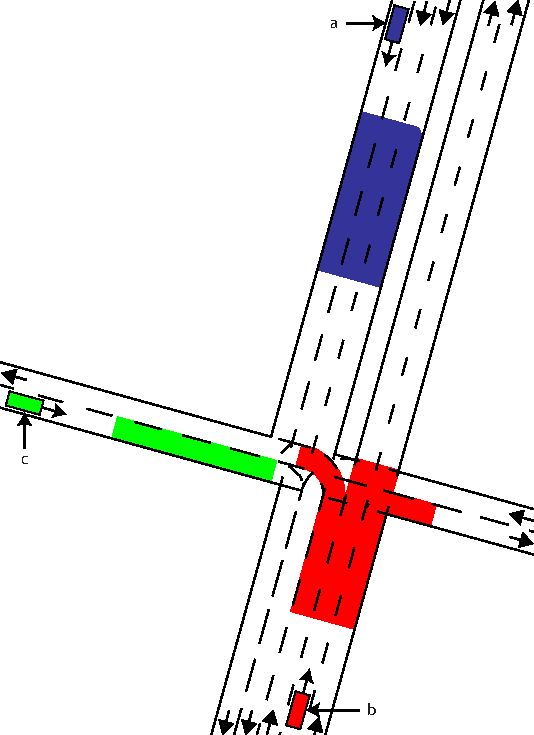
\includegraphics[width=0.4\columnwidth]{./figures/Scenario_Intersection_Occ_1,5-2,0s_final}
\caption{Occupancies of Obstacles~1, 2, and 3 in Scenario~I. The plot shows the initial configuration at $t_{0}$ and the predicted occupancies $\mathcal{O}(t)$ for ${t \in [t_{3}, t_{4}]}$.}
\label{fig:scenario1}
\end{figure}

\section{Math}
As an example, let us introduce $\mathcal{X}\subset\mathbb{R}^n$ as the set of feasible states $x$ and $\mathcal{U}\subset\mathbb{R}^m$ as the set of admissible control inputs $u$ of a system $f$, which is governed by the differential equation
\begin{equation}
	\begin{split}
	\dot{x}(t) &= f\big(x(t),u(t)\big). %\\
%	y&=g(x(t))
	\end{split}
	\label{eq:system}
\end{equation}

We assume that the initial time is $t_0 = 0$ and adhere to the notation $u([0, t_h])$ to describe a trajectory $u(t)\in\mathcal{U}$ for $t\in [0,t_h]$, $0<t_h$. Furthermore, $\chi\big(t_h,x(0),u([0,t_h])\big)\in\mathcal{X}$ denotes the solution of \eqref{eq:system} at time $t_h$ subject to $x(0)=x_0$ and $u([0,t_h])$.

Note that you should not reference an equation before introducing it. After giving the equation, you can refer to it, e.g., our system \eqref{eq:system} is awesome.


\section{Tables}
Tab.~\ref{tab:parameters} is an example of a nice table.

\begin{table}[!htb]\centering
\caption{Obstacle Parameters.}
\arstretch{1.3} 
\begin{tabular}{@{}llll@{}} \toprule
\textbf{Parameter} & \textbf{Variable} & \textbf{Parameter} &  \textbf{Variable} \\ \midrule
max. acceleration & $a_\mathrm{max}$ in $\unitfrac{m}{s^2}$ & Boolean for $C_\mathrm{back}$ & $b_\mathrm{back}$ \\ 
max. velocity & $v_\mathrm{max}$ in $\unitfrac{m}{s}$ & Boolean for $C_\mathrm{lane}$ & $b_\mathrm{lane}$ \\
switching velocity & $v_S$ in $\unitfrac{m}{s}$ & length & $l$ in $\unit{m}$ \\
speeding factor & $f_S$ & width & $w$ in $\unit{m}$ \\
\bottomrule
\end{tabular}
\label{tab:parameters}
\end{table}


\section{Algorithms}
Often, it will be helpful to describe your software by presenting pseudo code and explaining it (at least the significant lines). 

Alg.~\ref{alg:mainAlgorithm} shows the overall algorithm of \textit{SPOT}, which predicts the occupancy for a traffic participant up to the prediction horizon and can run in parallel for each traffic participant. First, the constraint management configures the parameters according to the set of last-measured states of the obstacle (line~\ref{alg:main_constraints}) as detailed in the next paragraph...

\begin{algorithm}
	\caption{Occupancy Prediction for an Obstacle}
	\begin{algorithmic}[1]
	\Require map
	\State parameters $\gets$ \Call{manageConstraints}{} \label{alg:main_constraints}
	\State reachableLanes $\gets$ \Call{reach}{map, parameters} \label{alg:main_reach}
	\ForAll{\Call{validAbstractions}{parameters}}
		\State $\mathcal{O}_{j}$ $\gets$ \Call{occupancy$_{j}$}{reachableLanes, parameters}\label{alg:main_abstractions}
	\EndFor
	\State \Return $\mathcal{O}$ $\gets$ \Call{intersect}{$\mathcal{O}_{j}$} \label{alg:main_intersect}
	\end{algorithmic}
	\label{alg:mainAlgorithm}
\end{algorithm}


\section{Citation} \label{sec:Citation}
For citations, we use a consecutively numbered citation style: bla \cite{latex} bla \cite{Koschi2017a, Althoff2017a} bla \cite{Paden2016}. To generate a bibliography file (the \texttt{.bib} file located in the folder content), you can use JabRef\footnote{\url{http://www.jabref.org/}}. Then, you run \textit{bibtex} and afterwards latex/pdflatex twice (as described in Sec.~\ref{sec:Using_this_template}).
% \chapter{Literature Review} \label{ch:lit_review}

To find relevant works, you should follow this guideline:
\begin{itemize}
\item Important catalogues: IEEE XPlore, Google scholar, Scopus, Web of Science, Research Gate
\item Start searching catalogues: Write down used keywords and used catalogues to avoid repeating a search; try some searches with the keyword ``survey'' or ``overview'' to find survey papers
\item Group results: Find categories in which to put your found papers
\item Rank papers in each category: consider reputation of journal/conference, reputation of authors, and citations 
\item In best ranked papers: Look into their literature lists; what other papers are relevant (do this iteratively)? Newer papers are more useful since they cover the literture up to a later point in time. Finding a great and recent survey paper is the jackpot
\item Once the search has converged: identify the most important groups
\item Visit websites of important groups to identify missed papers
\end{itemize}

\appendix{}
%\microtypesetup{protrusion=false}
% \glsaddall{} % add all defined terms to glossary, even if not referenced in text
% \printglossaries{} % TODO: uncomment if glossary needed
\listoffigures{}
\listoftables{}
\printbibliography{}

\end{document}